\documentclass{standalone}
\usepackage{tikz}
\begin{document}
% \documentclass[11pt, a4paper]{article}
% \usepackage{amsmath}
% \usepackage{tikz}
% \usepackage{geometry}
% \geometry{margin = 3cm}
% \usepackage{float, caption, subcaption}
% \begin{document}

\section{Fisher Waves}

The equation derived is of the form of a reaction-diffusion equation and as such it's solutions may consist of wave forms that propagate across the landscape the equation describes.

The common form of a  reaction diffusion equation is 

\begin{equation}
\frac{\partial}{\partial t} u = \frac{\partial ^2}{\partial x ^2} u + f(u) ,
\end{equation}

this is the common heat equation with the function $f(u)$ added on. 

For our equation, we see the combination of diffusion and advection in the flat mutation and fitness landscape and additional terms in the non-flat case. 

A Fisher wave connects two equilibrium from the dynamics. In our case, this is the initial starting point  and the final fixation condition. 

In solving these equations, the common substitution of $z = x + ct$ is used. 

\subsection{Wave Solution}

In Fisher's orginal paper the starting equation is used

\begin{equation}
\dot{p} = Dp'' + rp(1-p). 
\end{equation}

By using an ansatz of $\dot{p} = - v \frac{\partial p }{\partial x} $ the PDE can be reduced to an ODE

\begin{equation}
- v \frac{\mathrm{d}p}{\mathrm{d} x}  = D \frac{\mathrm{d} ^2 p}{\mathrm{d} x ^2} + rp(1-p)
\end{equation}

As there is no explicit $x$ dependence, we can use the substitution of a gradient $g = - \frac{\mathrm{d} p}{\mathrm{d} x}$.

\begin{align*}
g & = - \frac{\mathrm{d} p}{\mathrm{d} x} \\
\frac{\mathrm{d} g}{\mathrm{d} p} & = \frac{\mathrm{d} g}{\mathrm{d} x} \frac{\mathrm{d} x}{\mathrm{d} p} \\
& = - \frac{1}{g} \frac{\mathrm{d} g}{\mathrm{d} x} \\
& = \frac{1}{g} \frac{\partial^2 p}{\partial x^2}
\end{align*}

\begin{equation}
vg =  D g \frac{\partial g}{\partial p} + rp(1-p)
\end{equation}

We now take the limit 

$$\lim _{p \rightarrow 0} \frac{g}{p} = u$$

\begin{align*}
D \frac{g}{p} \frac{\partial g}{\partial p} - v \frac{g}{p} + r(1-p) & = 0 \\
D u ^2 - vu + r & = 0 
\end{align*}

Now this is a quadratic equation with solutions 

\begin{align*}
u & = \frac{v \pm \sqrt{v^2 - 4Dr}}{2D}
\end{align*}

This only has real roots for $v^2 - 4Dr \geq 0 $. 

Therefore, this traveling wave only exists for $v \geq 2 \sqrt{Dr}$.

\subsection{Initial Conditions that lead to traveling waves}

This is the KKP part of the analysis. 

\subsection{Stability Analysis}

Using the ODE; 

\begin{equation}
D \frac{\mathrm{d} ^2 U}{\mathrm{d} z^2} + v \frac{\mathrm{d} U}{\mathrm{d} z}  + rU(1-U) =0.
\end{equation}

By defining a new variable we can transform the second order single dimmension to two coupled first order differential equations. 

\begin{align}
V & = \frac{\mathrm{d} U}{\mathrm{d} z} \\
D \frac{\mathrm{d} V}{\mathrm{d} z} & = -v V + -rU(1-U) \\
\end{align}

If we rescale the dimensions such that $D=r=1$ we can reform the above into a matrix equation. 

\begin{equation}
\begin{pmatrix}
U' \\
V'
\end{pmatrix}
= 
\begin{pmatrix}
0 & 1 \\
-(1-U) & -v \\
\end{pmatrix}
\begin{pmatrix}
U \\
V
\end{pmatrix}
\end{equation}

The Jacobian of this system is 

\begin{equation}
J = 
\begin{pmatrix}
0 & 1 \\
-1 + 2U & -v
\end{pmatrix}
\end{equation}

We now take the usual approach for the stability analysis of the fixed points $A = (0,0)$ and $B = (1,0)$. 

\begin{align*}
-\lambda (-v - \lambda ) - (-1 + 2U) & = 0 \\
\lambda ^2 + v \lambda + (1- 2U) & = 0 \\
\lambda & = \frac{-v \pm \sqrt{v^2 - 4 (1-2U) }}{2}
\end{align*}

Point A $(0,0)$.

\begin{align*}
\lambda & = -\frac{v}{2} + \frac{1}{2} \sqrt{v^2 - 4} \\
\lambda & = -\frac{v}{2} - \frac{1}{2} \sqrt{v^2 - 4} \\
\end{align*}

If $v < 2$ then this is a stable spiral. 

If $v > 2$ then this is a stable node 

Point B $(1,0)$

\begin{align*}
\lambda & = -\frac{v}{2} + \frac{1}{2} \sqrt{v^2 + 4} \\
\lambda & = -\frac{v}{2} - \frac{1}{2} \sqrt{v^2 + 4} \\
\end{align*}

Therefore, this is a saddle point for all $v$. 

We can see this by looking at the phase portrait of the system. 

\begin{figure}[H]
\begin{subfigure}[h]{0.5\textwidth}
% Created by tikzDevice version 0.7.0 on 2015-03-09 16:57:45
% !TEX encoding = UTF-8 Unicode
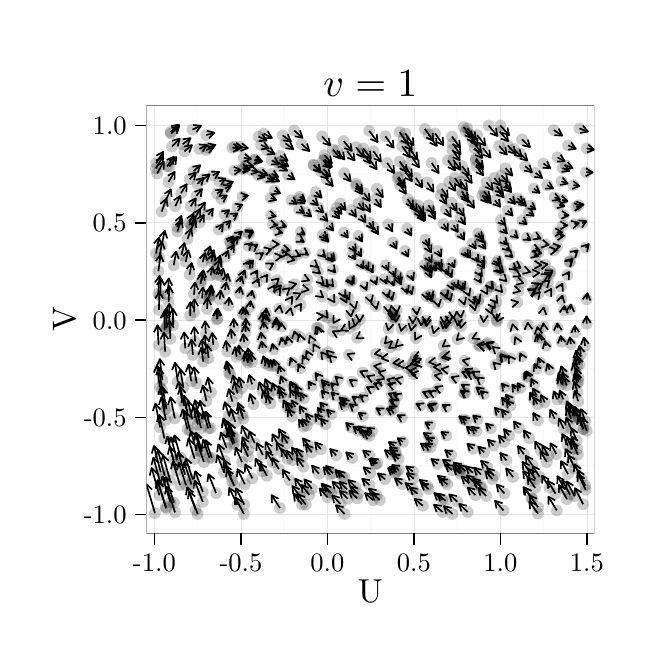
\begin{tikzpicture}[x=1pt,y=1pt]
\definecolor[named]{fillColor}{rgb}{1.00,1.00,1.00}
\path[use as bounding box,fill=fillColor,fill opacity=0.00] (0,0) rectangle (216.81,216.81);
\begin{scope}
\path[clip] (  0.00,  0.00) rectangle (216.81,216.81);
\definecolor[named]{drawColor}{rgb}{1.00,1.00,1.00}
\definecolor[named]{fillColor}{rgb}{1.00,1.00,1.00}

\path[draw=drawColor,line width= 0.6pt,line join=round,line cap=round,fill=fillColor] ( -0.00,  0.00) rectangle (216.81,216.81);
\end{scope}
\begin{scope}
\path[clip] ( 42.89, 34.03) rectangle (204.76,188.82);
\definecolor[named]{fillColor}{rgb}{1.00,1.00,1.00}

\path[fill=fillColor] ( 42.89, 34.03) rectangle (204.76,188.82);
\definecolor[named]{drawColor}{rgb}{0.98,0.98,0.98}

\path[draw=drawColor,line width= 0.6pt,line join=round] ( 42.89, 58.42) --
	(204.76, 58.42);

\path[draw=drawColor,line width= 0.6pt,line join=round] ( 42.89, 93.57) --
	(204.76, 93.57);

\path[draw=drawColor,line width= 0.6pt,line join=round] ( 42.89,128.73) --
	(204.76,128.73);

\path[draw=drawColor,line width= 0.6pt,line join=round] ( 42.89,163.89) --
	(204.76,163.89);

\path[draw=drawColor,line width= 0.6pt,line join=round] ( 61.42, 34.03) --
	( 61.42,188.82);

\path[draw=drawColor,line width= 0.6pt,line join=round] ( 92.68, 34.03) --
	( 92.68,188.82);

\path[draw=drawColor,line width= 0.6pt,line join=round] (123.94, 34.03) --
	(123.94,188.82);

\path[draw=drawColor,line width= 0.6pt,line join=round] (155.19, 34.03) --
	(155.19,188.82);

\path[draw=drawColor,line width= 0.6pt,line join=round] (186.45, 34.03) --
	(186.45,188.82);
\definecolor[named]{drawColor}{rgb}{0.90,0.90,0.90}

\path[draw=drawColor,line width= 0.2pt,line join=round] ( 42.89, 40.84) --
	(204.76, 40.84);

\path[draw=drawColor,line width= 0.2pt,line join=round] ( 42.89, 76.00) --
	(204.76, 76.00);

\path[draw=drawColor,line width= 0.2pt,line join=round] ( 42.89,111.15) --
	(204.76,111.15);

\path[draw=drawColor,line width= 0.2pt,line join=round] ( 42.89,146.31) --
	(204.76,146.31);

\path[draw=drawColor,line width= 0.2pt,line join=round] ( 42.89,181.46) --
	(204.76,181.46);

\path[draw=drawColor,line width= 0.2pt,line join=round] ( 45.79, 34.03) --
	( 45.79,188.82);

\path[draw=drawColor,line width= 0.2pt,line join=round] ( 77.05, 34.03) --
	( 77.05,188.82);

\path[draw=drawColor,line width= 0.2pt,line join=round] (108.31, 34.03) --
	(108.31,188.82);

\path[draw=drawColor,line width= 0.2pt,line join=round] (139.56, 34.03) --
	(139.56,188.82);

\path[draw=drawColor,line width= 0.2pt,line join=round] (170.82, 34.03) --
	(170.82,188.82);

\path[draw=drawColor,line width= 0.2pt,line join=round] (202.08, 34.03) --
	(202.08,188.82);
\definecolor[named]{fillColor}{rgb}{0.00,0.00,0.00}

\path[fill=fillColor,fill opacity=0.20] (170.82,181.46) circle (  2.13);

\path[fill=fillColor,fill opacity=0.20] (163.42,141.08) circle (  2.13);

\path[fill=fillColor,fill opacity=0.20] (100.70,150.05) circle (  2.13);

\path[fill=fillColor,fill opacity=0.20] (182.34, 58.69) circle (  2.13);

\path[fill=fillColor,fill opacity=0.20] (144.42,160.89) circle (  2.13);

\path[fill=fillColor,fill opacity=0.20] ( 56.01,174.67) circle (  2.13);

\path[fill=fillColor,fill opacity=0.20] (114.01, 82.03) circle (  2.13);

\path[fill=fillColor,fill opacity=0.20] (195.96, 48.10) circle (  2.13);

\path[fill=fillColor,fill opacity=0.20] (149.91, 41.81) circle (  2.13);

\path[fill=fillColor,fill opacity=0.20] ( 95.64, 95.89) circle (  2.13);

\path[fill=fillColor,fill opacity=0.20] ( 93.54,136.59) circle (  2.13);

\path[fill=fillColor,fill opacity=0.20] ( 99.36, 50.22) circle (  2.13);

\path[fill=fillColor,fill opacity=0.20] ( 71.15, 60.34) circle (  2.13);

\path[fill=fillColor,fill opacity=0.20] ( 65.65, 61.43) circle (  2.13);

\path[fill=fillColor,fill opacity=0.20] (184.05,141.19) circle (  2.13);

\path[fill=fillColor,fill opacity=0.20] (146.63,130.96) circle (  2.13);

\path[fill=fillColor,fill opacity=0.20] (167.61,123.22) circle (  2.13);

\path[fill=fillColor,fill opacity=0.20] ( 80.06,142.23) circle (  2.13);

\path[fill=fillColor,fill opacity=0.20] (130.88, 89.40) circle (  2.13);

\path[fill=fillColor,fill opacity=0.20] ( 98.97,174.80) circle (  2.13);

\path[fill=fillColor,fill opacity=0.20] (133.30, 56.23) circle (  2.13);

\path[fill=fillColor,fill opacity=0.20] (160.86, 56.00) circle (  2.13);

\path[fill=fillColor,fill opacity=0.20] ( 84.92,101.06) circle (  2.13);

\path[fill=fillColor,fill opacity=0.20] ( 96.13, 83.73) circle (  2.13);

\path[fill=fillColor,fill opacity=0.20] (146.27, 67.34) circle (  2.13);

\path[fill=fillColor,fill opacity=0.20] ( 56.58, 80.08) circle (  2.13);

\path[fill=fillColor,fill opacity=0.20] (190.06,136.34) circle (  2.13);

\path[fill=fillColor,fill opacity=0.20] ( 48.69, 89.42) circle (  2.13);

\path[fill=fillColor,fill opacity=0.20] ( 88.56,162.38) circle (  2.13);

\path[fill=fillColor,fill opacity=0.20] (156.64,108.86) circle (  2.13);

\path[fill=fillColor,fill opacity=0.20] (168.53, 54.92) circle (  2.13);

\path[fill=fillColor,fill opacity=0.20] ( 72.57, 69.68) circle (  2.13);

\path[fill=fillColor,fill opacity=0.20] ( 50.36,166.66) circle (  2.13);

\path[fill=fillColor,fill opacity=0.20] (129.28,177.53) circle (  2.13);

\path[fill=fillColor,fill opacity=0.20] ( 54.23, 88.95) circle (  2.13);

\path[fill=fillColor,fill opacity=0.20] ( 84.97, 62.42) circle (  2.13);

\path[fill=fillColor,fill opacity=0.20] ( 53.26, 41.66) circle (  2.13);

\path[fill=fillColor,fill opacity=0.20] (153.41,172.66) circle (  2.13);

\path[fill=fillColor,fill opacity=0.20] (187.52,127.29) circle (  2.13);

\path[fill=fillColor,fill opacity=0.20] ( 65.25,149.23) circle (  2.13);

\path[fill=fillColor,fill opacity=0.20] (109.62, 97.73) circle (  2.13);

\path[fill=fillColor,fill opacity=0.20] ( 80.12, 97.94) circle (  2.13);

\path[fill=fillColor,fill opacity=0.20] ( 49.93, 75.07) circle (  2.13);

\path[fill=fillColor,fill opacity=0.20] (151.09,151.25) circle (  2.13);

\path[fill=fillColor,fill opacity=0.20] (144.59,137.84) circle (  2.13);

\path[fill=fillColor,fill opacity=0.20] (191.68,142.89) circle (  2.13);

\path[fill=fillColor,fill opacity=0.20] (133.11, 62.60) circle (  2.13);

\path[fill=fillColor,fill opacity=0.20] (168.86,154.36) circle (  2.13);

\path[fill=fillColor,fill opacity=0.20] (114.35,164.23) circle (  2.13);

\path[fill=fillColor,fill opacity=0.20] (194.98,127.45) circle (  2.13);

\path[fill=fillColor,fill opacity=0.20] (200.73, 44.59) circle (  2.13);

\path[fill=fillColor,fill opacity=0.20] (170.30, 77.81) circle (  2.13);

\path[fill=fillColor,fill opacity=0.20] (138.76,170.18) circle (  2.13);

\path[fill=fillColor,fill opacity=0.20] (163.64, 51.26) circle (  2.13);

\path[fill=fillColor,fill opacity=0.20] ( 86.47, 54.86) circle (  2.13);

\path[fill=fillColor,fill opacity=0.20] (107.34,169.29) circle (  2.13);

\path[fill=fillColor,fill opacity=0.20] (169.47,159.35) circle (  2.13);

\path[fill=fillColor,fill opacity=0.20] ( 85.86, 95.58) circle (  2.13);

\path[fill=fillColor,fill opacity=0.20] ( 64.35,106.24) circle (  2.13);

\path[fill=fillColor,fill opacity=0.20] (172.88, 76.87) circle (  2.13);

\path[fill=fillColor,fill opacity=0.20] (110.53,110.17) circle (  2.13);

\path[fill=fillColor,fill opacity=0.20] ( 52.77,130.99) circle (  2.13);

\path[fill=fillColor,fill opacity=0.20] ( 55.25, 61.49) circle (  2.13);

\path[fill=fillColor,fill opacity=0.20] (151.11,129.58) circle (  2.13);

\path[fill=fillColor,fill opacity=0.20] ( 59.20, 51.82) circle (  2.13);

\path[fill=fillColor,fill opacity=0.20] (158.33,179.35) circle (  2.13);

\path[fill=fillColor,fill opacity=0.20] (202.04, 71.15) circle (  2.13);

\path[fill=fillColor,fill opacity=0.20] (106.62, 98.81) circle (  2.13);

\path[fill=fillColor,fill opacity=0.20] (129.00,125.86) circle (  2.13);

\path[fill=fillColor,fill opacity=0.20] (146.58, 80.20) circle (  2.13);

\path[fill=fillColor,fill opacity=0.20] (161.86,133.79) circle (  2.13);

\path[fill=fillColor,fill opacity=0.20] ( 54.03,144.75) circle (  2.13);

\path[fill=fillColor,fill opacity=0.20] ( 48.37,138.12) circle (  2.13);

\path[fill=fillColor,fill opacity=0.20] (159.73, 91.56) circle (  2.13);

\path[fill=fillColor,fill opacity=0.20] (153.58,174.87) circle (  2.13);

\path[fill=fillColor,fill opacity=0.20] (192.90,118.68) circle (  2.13);

\path[fill=fillColor,fill opacity=0.20] (197.87,106.72) circle (  2.13);

\path[fill=fillColor,fill opacity=0.20] (155.39,104.25) circle (  2.13);

\path[fill=fillColor,fill opacity=0.20] (131.23, 62.50) circle (  2.13);

\path[fill=fillColor,fill opacity=0.20] (117.36,137.76) circle (  2.13);

\path[fill=fillColor,fill opacity=0.20] ( 59.12,144.01) circle (  2.13);

\path[fill=fillColor,fill opacity=0.20] (180.38, 90.59) circle (  2.13);

\path[fill=fillColor,fill opacity=0.20] (114.11, 80.12) circle (  2.13);

\path[fill=fillColor,fill opacity=0.20] (107.64, 73.52) circle (  2.13);

\path[fill=fillColor,fill opacity=0.20] (132.75, 95.68) circle (  2.13);

\path[fill=fillColor,fill opacity=0.20] ( 94.10,163.60) circle (  2.13);

\path[fill=fillColor,fill opacity=0.20] (160.99,104.62) circle (  2.13);

\path[fill=fillColor,fill opacity=0.20] (161.46, 92.02) circle (  2.13);

\path[fill=fillColor,fill opacity=0.20] ( 73.42,139.05) circle (  2.13);

\path[fill=fillColor,fill opacity=0.20] ( 98.57, 93.78) circle (  2.13);

\path[fill=fillColor,fill opacity=0.20] ( 79.81,142.77) circle (  2.13);

\path[fill=fillColor,fill opacity=0.20] (114.55, 54.19) circle (  2.13);

\path[fill=fillColor,fill opacity=0.20] ( 47.20,120.83) circle (  2.13);

\path[fill=fillColor,fill opacity=0.20] (139.17, 95.54) circle (  2.13);

\path[fill=fillColor,fill opacity=0.20] (192.79, 89.20) circle (  2.13);

\path[fill=fillColor,fill opacity=0.20] (113.70, 54.41) circle (  2.13);

\path[fill=fillColor,fill opacity=0.20] ( 85.34,108.44) circle (  2.13);

\path[fill=fillColor,fill opacity=0.20] (102.70, 50.20) circle (  2.13);

\path[fill=fillColor,fill opacity=0.20] ( 64.61, 81.88) circle (  2.13);

\path[fill=fillColor,fill opacity=0.20] (157.60, 84.80) circle (  2.13);

\path[fill=fillColor,fill opacity=0.20] (164.84, 84.41) circle (  2.13);

\path[fill=fillColor,fill opacity=0.20] ( 49.80,154.18) circle (  2.13);

\path[fill=fillColor,fill opacity=0.20] (194.72, 87.58) circle (  2.13);

\path[fill=fillColor,fill opacity=0.20] ( 98.22,120.53) circle (  2.13);

\path[fill=fillColor,fill opacity=0.20] ( 91.15, 43.24) circle (  2.13);

\path[fill=fillColor,fill opacity=0.20] ( 57.11,132.19) circle (  2.13);

\path[fill=fillColor,fill opacity=0.20] (106.73,168.88) circle (  2.13);

\path[fill=fillColor,fill opacity=0.20] ( 96.62,106.04) circle (  2.13);

\path[fill=fillColor,fill opacity=0.20] (152.43,119.27) circle (  2.13);

\path[fill=fillColor,fill opacity=0.20] (145.36, 73.15) circle (  2.13);

\path[fill=fillColor,fill opacity=0.20] (173.47,150.72) circle (  2.13);

\path[fill=fillColor,fill opacity=0.20] (185.46, 63.88) circle (  2.13);

\path[fill=fillColor,fill opacity=0.20] (134.38,179.09) circle (  2.13);

\path[fill=fillColor,fill opacity=0.20] ( 86.94,136.42) circle (  2.13);

\path[fill=fillColor,fill opacity=0.20] (135.31, 51.87) circle (  2.13);

\path[fill=fillColor,fill opacity=0.20] ( 96.02, 86.77) circle (  2.13);

\path[fill=fillColor,fill opacity=0.20] (104.92, 90.77) circle (  2.13);

\path[fill=fillColor,fill opacity=0.20] (168.57,115.76) circle (  2.13);

\path[fill=fillColor,fill opacity=0.20] (132.00,139.20) circle (  2.13);

\path[fill=fillColor,fill opacity=0.20] ( 69.98,127.01) circle (  2.13);

\path[fill=fillColor,fill opacity=0.20] ( 69.24,161.24) circle (  2.13);

\path[fill=fillColor,fill opacity=0.20] (157.85, 96.44) circle (  2.13);

\path[fill=fillColor,fill opacity=0.20] (144.34, 51.26) circle (  2.13);

\path[fill=fillColor,fill opacity=0.20] ( 58.91,152.25) circle (  2.13);

\path[fill=fillColor,fill opacity=0.20] (164.74,110.71) circle (  2.13);

\path[fill=fillColor,fill opacity=0.20] ( 79.71, 64.10) circle (  2.13);

\path[fill=fillColor,fill opacity=0.20] ( 65.56,118.89) circle (  2.13);

\path[fill=fillColor,fill opacity=0.20] ( 51.55,104.38) circle (  2.13);

\path[fill=fillColor,fill opacity=0.20] (148.15, 59.17) circle (  2.13);

\path[fill=fillColor,fill opacity=0.20] (167.95, 53.72) circle (  2.13);

\path[fill=fillColor,fill opacity=0.20] (144.87,152.64) circle (  2.13);

\path[fill=fillColor,fill opacity=0.20] (177.35,127.34) circle (  2.13);

\path[fill=fillColor,fill opacity=0.20] (146.04, 79.75) circle (  2.13);

\path[fill=fillColor,fill opacity=0.20] (107.60, 87.27) circle (  2.13);

\path[fill=fillColor,fill opacity=0.20] (116.40,108.24) circle (  2.13);

\path[fill=fillColor,fill opacity=0.20] (128.49, 97.41) circle (  2.13);

\path[fill=fillColor,fill opacity=0.20] (153.84,169.07) circle (  2.13);

\path[fill=fillColor,fill opacity=0.20] ( 92.13, 63.32) circle (  2.13);

\path[fill=fillColor,fill opacity=0.20] ( 79.21, 96.57) circle (  2.13);

\path[fill=fillColor,fill opacity=0.20] ( 69.09,143.83) circle (  2.13);

\path[fill=fillColor,fill opacity=0.20] ( 99.61, 58.12) circle (  2.13);

\path[fill=fillColor,fill opacity=0.20] ( 66.25, 84.98) circle (  2.13);

\path[fill=fillColor,fill opacity=0.20] (102.65, 63.38) circle (  2.13);

\path[fill=fillColor,fill opacity=0.20] (170.58,179.24) circle (  2.13);

\path[fill=fillColor,fill opacity=0.20] ( 78.55,113.08) circle (  2.13);

\path[fill=fillColor,fill opacity=0.20] (106.65,148.74) circle (  2.13);

\path[fill=fillColor,fill opacity=0.20] (156.40,148.24) circle (  2.13);

\path[fill=fillColor,fill opacity=0.20] (172.58,159.74) circle (  2.13);

\path[fill=fillColor,fill opacity=0.20] ( 63.27, 45.43) circle (  2.13);

\path[fill=fillColor,fill opacity=0.20] ( 73.72,104.44) circle (  2.13);

\path[fill=fillColor,fill opacity=0.20] ( 84.56,104.48) circle (  2.13);

\path[fill=fillColor,fill opacity=0.20] ( 56.24, 86.81) circle (  2.13);

\path[fill=fillColor,fill opacity=0.20] ( 61.43, 41.09) circle (  2.13);

\path[fill=fillColor,fill opacity=0.20] (101.05,125.73) circle (  2.13);

\path[fill=fillColor,fill opacity=0.20] (134.49,160.10) circle (  2.13);

\path[fill=fillColor,fill opacity=0.20] (154.36,162.48) circle (  2.13);

\path[fill=fillColor,fill opacity=0.20] (150.89,120.47) circle (  2.13);

\path[fill=fillColor,fill opacity=0.20] ( 68.42,156.88) circle (  2.13);

\path[fill=fillColor,fill opacity=0.20] (145.68,119.07) circle (  2.13);

\path[fill=fillColor,fill opacity=0.20] (174.14,134.82) circle (  2.13);

\path[fill=fillColor,fill opacity=0.20] ( 74.19,148.59) circle (  2.13);

\path[fill=fillColor,fill opacity=0.20] (106.36,124.82) circle (  2.13);

\path[fill=fillColor,fill opacity=0.20] (164.04,131.34) circle (  2.13);

\path[fill=fillColor,fill opacity=0.20] (197.58,145.83) circle (  2.13);

\path[fill=fillColor,fill opacity=0.20] (163.18, 89.73) circle (  2.13);

\path[fill=fillColor,fill opacity=0.20] ( 70.94, 56.24) circle (  2.13);

\path[fill=fillColor,fill opacity=0.20] (163.33,128.29) circle (  2.13);

\path[fill=fillColor,fill opacity=0.20] (107.37,140.89) circle (  2.13);

\path[fill=fillColor,fill opacity=0.20] (150.32, 97.71) circle (  2.13);

\path[fill=fillColor,fill opacity=0.20] ( 82.85,124.70) circle (  2.13);

\path[fill=fillColor,fill opacity=0.20] (133.34,114.74) circle (  2.13);

\path[fill=fillColor,fill opacity=0.20] ( 95.98, 86.84) circle (  2.13);

\path[fill=fillColor,fill opacity=0.20] ( 84.89,111.98) circle (  2.13);

\path[fill=fillColor,fill opacity=0.20] (177.48,121.74) circle (  2.13);

\path[fill=fillColor,fill opacity=0.20] (176.50,104.29) circle (  2.13);

\path[fill=fillColor,fill opacity=0.20] (139.50, 91.58) circle (  2.13);

\path[fill=fillColor,fill opacity=0.20] ( 74.55,108.49) circle (  2.13);

\path[fill=fillColor,fill opacity=0.20] (117.33, 88.87) circle (  2.13);

\path[fill=fillColor,fill opacity=0.20] ( 47.82,119.94) circle (  2.13);

\path[fill=fillColor,fill opacity=0.20] (131.01,101.32) circle (  2.13);

\path[fill=fillColor,fill opacity=0.20] ( 55.07, 51.51) circle (  2.13);

\path[fill=fillColor,fill opacity=0.20] (125.92, 98.98) circle (  2.13);

\path[fill=fillColor,fill opacity=0.20] ( 77.64,155.79) circle (  2.13);

\path[fill=fillColor,fill opacity=0.20] (174.45, 80.28) circle (  2.13);

\path[fill=fillColor,fill opacity=0.20] ( 98.49, 47.34) circle (  2.13);

\path[fill=fillColor,fill opacity=0.20] (140.88, 48.37) circle (  2.13);

\path[fill=fillColor,fill opacity=0.20] (122.22,131.00) circle (  2.13);

\path[fill=fillColor,fill opacity=0.20] (165.67,121.36) circle (  2.13);

\path[fill=fillColor,fill opacity=0.20] ( 52.13,173.85) circle (  2.13);

\path[fill=fillColor,fill opacity=0.20] (114.54, 41.07) circle (  2.13);

\path[fill=fillColor,fill opacity=0.20] ( 45.99, 41.40) circle (  2.13);

\path[fill=fillColor,fill opacity=0.20] (182.41, 46.57) circle (  2.13);

\path[fill=fillColor,fill opacity=0.20] (151.04,120.38) circle (  2.13);

\path[fill=fillColor,fill opacity=0.20] ( 64.96,134.87) circle (  2.13);

\path[fill=fillColor,fill opacity=0.20] ( 98.10,151.12) circle (  2.13);

\path[fill=fillColor,fill opacity=0.20] (131.62, 84.06) circle (  2.13);

\path[fill=fillColor,fill opacity=0.20] ( 46.38,135.23) circle (  2.13);

\path[fill=fillColor,fill opacity=0.20] ( 58.71,112.71) circle (  2.13);

\path[fill=fillColor,fill opacity=0.20] (132.52, 65.63) circle (  2.13);

\path[fill=fillColor,fill opacity=0.20] ( 57.77,140.44) circle (  2.13);

\path[fill=fillColor,fill opacity=0.20] ( 84.35,164.37) circle (  2.13);

\path[fill=fillColor,fill opacity=0.20] (114.30,142.81) circle (  2.13);

\path[fill=fillColor,fill opacity=0.20] ( 85.27,178.55) circle (  2.13);

\path[fill=fillColor,fill opacity=0.20] (195.23, 55.48) circle (  2.13);

\path[fill=fillColor,fill opacity=0.20] ( 89.84,110.60) circle (  2.13);

\path[fill=fillColor,fill opacity=0.20] (183.81,136.80) circle (  2.13);

\path[fill=fillColor,fill opacity=0.20] ( 60.14,113.98) circle (  2.13);

\path[fill=fillColor,fill opacity=0.20] (163.84, 55.32) circle (  2.13);

\path[fill=fillColor,fill opacity=0.20] ( 61.48, 73.43) circle (  2.13);

\path[fill=fillColor,fill opacity=0.20] ( 91.59, 92.41) circle (  2.13);

\path[fill=fillColor,fill opacity=0.20] ( 66.12, 72.12) circle (  2.13);

\path[fill=fillColor,fill opacity=0.20] (181.64,152.50) circle (  2.13);

\path[fill=fillColor,fill opacity=0.20] (202.00,109.85) circle (  2.13);

\path[fill=fillColor,fill opacity=0.20] (173.00, 60.46) circle (  2.13);

\path[fill=fillColor,fill opacity=0.20] ( 72.12, 99.81) circle (  2.13);

\path[fill=fillColor,fill opacity=0.20] ( 61.05, 63.95) circle (  2.13);

\path[fill=fillColor,fill opacity=0.20] ( 91.28,166.70) circle (  2.13);

\path[fill=fillColor,fill opacity=0.20] (199.02, 88.89) circle (  2.13);

\path[fill=fillColor,fill opacity=0.20] (164.88,157.65) circle (  2.13);

\path[fill=fillColor,fill opacity=0.20] ( 80.35,115.95) circle (  2.13);

\path[fill=fillColor,fill opacity=0.20] ( 90.94,115.32) circle (  2.13);

\path[fill=fillColor,fill opacity=0.20] (172.67, 81.51) circle (  2.13);

\path[fill=fillColor,fill opacity=0.20] (153.90,145.38) circle (  2.13);

\path[fill=fillColor,fill opacity=0.20] (133.59, 83.72) circle (  2.13);

\path[fill=fillColor,fill opacity=0.20] (134.43,168.45) circle (  2.13);

\path[fill=fillColor,fill opacity=0.20] ( 52.70, 60.62) circle (  2.13);

\path[fill=fillColor,fill opacity=0.20] ( 75.52, 97.89) circle (  2.13);

\path[fill=fillColor,fill opacity=0.20] (125.91, 94.45) circle (  2.13);

\path[fill=fillColor,fill opacity=0.20] (187.00,131.18) circle (  2.13);

\path[fill=fillColor,fill opacity=0.20] (153.32,177.46) circle (  2.13);

\path[fill=fillColor,fill opacity=0.20] ( 97.38,134.73) circle (  2.13);

\path[fill=fillColor,fill opacity=0.20] (134.03,162.92) circle (  2.13);

\path[fill=fillColor,fill opacity=0.20] ( 50.93,117.59) circle (  2.13);

\path[fill=fillColor,fill opacity=0.20] (110.88,149.93) circle (  2.13);

\path[fill=fillColor,fill opacity=0.20] (125.74, 59.12) circle (  2.13);

\path[fill=fillColor,fill opacity=0.20] (197.64, 47.52) circle (  2.13);

\path[fill=fillColor,fill opacity=0.20] ( 97.86, 85.42) circle (  2.13);

\path[fill=fillColor,fill opacity=0.20] ( 48.05, 56.25) circle (  2.13);

\path[fill=fillColor,fill opacity=0.20] (198.06, 92.49) circle (  2.13);

\path[fill=fillColor,fill opacity=0.20] (140.27,162.56) circle (  2.13);

\path[fill=fillColor,fill opacity=0.20] ( 62.02,173.02) circle (  2.13);

\path[fill=fillColor,fill opacity=0.20] ( 83.36,163.47) circle (  2.13);

\path[fill=fillColor,fill opacity=0.20] (137.14,144.20) circle (  2.13);

\path[fill=fillColor,fill opacity=0.20] (176.25, 86.26) circle (  2.13);

\path[fill=fillColor,fill opacity=0.20] (143.72,140.24) circle (  2.13);

\path[fill=fillColor,fill opacity=0.20] (144.01, 84.68) circle (  2.13);

\path[fill=fillColor,fill opacity=0.20] (119.57,153.42) circle (  2.13);

\path[fill=fillColor,fill opacity=0.20] (108.36,112.06) circle (  2.13);

\path[fill=fillColor,fill opacity=0.20] (106.87,112.67) circle (  2.13);

\path[fill=fillColor,fill opacity=0.20] (201.53, 74.55) circle (  2.13);

\path[fill=fillColor,fill opacity=0.20] ( 66.36,132.30) circle (  2.13);

\path[fill=fillColor,fill opacity=0.20] (175.75,142.10) circle (  2.13);

\path[fill=fillColor,fill opacity=0.20] (118.64, 82.56) circle (  2.13);

\path[fill=fillColor,fill opacity=0.20] ( 61.34,160.36) circle (  2.13);

\path[fill=fillColor,fill opacity=0.20] ( 92.43, 88.62) circle (  2.13);

\path[fill=fillColor,fill opacity=0.20] ( 53.33,152.30) circle (  2.13);

\path[fill=fillColor,fill opacity=0.20] (172.71,166.00) circle (  2.13);

\path[fill=fillColor,fill opacity=0.20] (186.30,114.77) circle (  2.13);

\path[fill=fillColor,fill opacity=0.20] (135.10,107.92) circle (  2.13);

\path[fill=fillColor,fill opacity=0.20] (166.58,181.42) circle (  2.13);

\path[fill=fillColor,fill opacity=0.20] (170.34,174.11) circle (  2.13);

\path[fill=fillColor,fill opacity=0.20] (143.37,130.97) circle (  2.13);

\path[fill=fillColor,fill opacity=0.20] (131.25, 78.39) circle (  2.13);

\path[fill=fillColor,fill opacity=0.20] (194.21, 89.34) circle (  2.13);

\path[fill=fillColor,fill opacity=0.20] ( 56.88, 55.27) circle (  2.13);

\path[fill=fillColor,fill opacity=0.20] ( 88.70,122.81) circle (  2.13);

\path[fill=fillColor,fill opacity=0.20] ( 97.69, 61.91) circle (  2.13);

\path[fill=fillColor,fill opacity=0.20] (132.20, 79.07) circle (  2.13);

\path[fill=fillColor,fill opacity=0.20] (170.21,129.03) circle (  2.13);

\path[fill=fillColor,fill opacity=0.20] ( 71.07,149.46) circle (  2.13);

\path[fill=fillColor,fill opacity=0.20] (116.78,112.94) circle (  2.13);

\path[fill=fillColor,fill opacity=0.20] (121.90,123.27) circle (  2.13);

\path[fill=fillColor,fill opacity=0.20] (150.79, 52.75) circle (  2.13);

\path[fill=fillColor,fill opacity=0.20] (183.02,121.66) circle (  2.13);

\path[fill=fillColor,fill opacity=0.20] (145.61,120.36) circle (  2.13);

\path[fill=fillColor,fill opacity=0.20] (119.99,111.19) circle (  2.13);

\path[fill=fillColor,fill opacity=0.20] ( 81.62, 80.74) circle (  2.13);

\path[fill=fillColor,fill opacity=0.20] ( 66.53, 61.34) circle (  2.13);

\path[fill=fillColor,fill opacity=0.20] (147.96, 91.00) circle (  2.13);

\path[fill=fillColor,fill opacity=0.20] ( 46.44,167.82) circle (  2.13);

\path[fill=fillColor,fill opacity=0.20] (165.82,102.44) circle (  2.13);

\path[fill=fillColor,fill opacity=0.20] ( 62.87,125.46) circle (  2.13);

\path[fill=fillColor,fill opacity=0.20] (138.05,173.11) circle (  2.13);

\path[fill=fillColor,fill opacity=0.20] (150.47,110.69) circle (  2.13);

\path[fill=fillColor,fill opacity=0.20] ( 98.16,154.77) circle (  2.13);

\path[fill=fillColor,fill opacity=0.20] (186.38,167.72) circle (  2.13);

\path[fill=fillColor,fill opacity=0.20] ( 62.49,124.28) circle (  2.13);

\path[fill=fillColor,fill opacity=0.20] (103.40,167.06) circle (  2.13);

\path[fill=fillColor,fill opacity=0.20] (187.08,138.54) circle (  2.13);

\path[fill=fillColor,fill opacity=0.20] (166.19, 57.90) circle (  2.13);

\path[fill=fillColor,fill opacity=0.20] ( 52.85, 45.19) circle (  2.13);

\path[fill=fillColor,fill opacity=0.20] (112.88, 49.96) circle (  2.13);

\path[fill=fillColor,fill opacity=0.20] ( 94.74, 53.17) circle (  2.13);

\path[fill=fillColor,fill opacity=0.20] (121.52,157.04) circle (  2.13);

\path[fill=fillColor,fill opacity=0.20] (154.73,124.10) circle (  2.13);

\path[fill=fillColor,fill opacity=0.20] ( 49.42, 68.37) circle (  2.13);

\path[fill=fillColor,fill opacity=0.20] ( 82.22,127.80) circle (  2.13);

\path[fill=fillColor,fill opacity=0.20] (193.74,149.11) circle (  2.13);

\path[fill=fillColor,fill opacity=0.20] (187.96,124.90) circle (  2.13);

\path[fill=fillColor,fill opacity=0.20] (140.54,151.18) circle (  2.13);

\path[fill=fillColor,fill opacity=0.20] ( 91.01,123.05) circle (  2.13);

\path[fill=fillColor,fill opacity=0.20] (109.25,133.53) circle (  2.13);

\path[fill=fillColor,fill opacity=0.20] (141.86, 80.19) circle (  2.13);

\path[fill=fillColor,fill opacity=0.20] (131.68,112.25) circle (  2.13);

\path[fill=fillColor,fill opacity=0.20] ( 78.99,167.10) circle (  2.13);

\path[fill=fillColor,fill opacity=0.20] (105.05,108.26) circle (  2.13);

\path[fill=fillColor,fill opacity=0.20] (157.23,156.73) circle (  2.13);

\path[fill=fillColor,fill opacity=0.20] (157.96,135.66) circle (  2.13);

\path[fill=fillColor,fill opacity=0.20] (106.65,141.96) circle (  2.13);

\path[fill=fillColor,fill opacity=0.20] (184.32,104.71) circle (  2.13);

\path[fill=fillColor,fill opacity=0.20] (150.41, 93.33) circle (  2.13);

\path[fill=fillColor,fill opacity=0.20] (113.04, 44.69) circle (  2.13);

\path[fill=fillColor,fill opacity=0.20] (100.02, 96.96) circle (  2.13);

\path[fill=fillColor,fill opacity=0.20] (162.24, 71.02) circle (  2.13);

\path[fill=fillColor,fill opacity=0.20] (198.56, 94.75) circle (  2.13);

\path[fill=fillColor,fill opacity=0.20] (184.24,124.07) circle (  2.13);

\path[fill=fillColor,fill opacity=0.20] (185.23, 95.70) circle (  2.13);

\path[fill=fillColor,fill opacity=0.20] (144.09, 65.09) circle (  2.13);

\path[fill=fillColor,fill opacity=0.20] ( 79.66, 61.82) circle (  2.13);

\path[fill=fillColor,fill opacity=0.20] ( 79.55,131.23) circle (  2.13);

\path[fill=fillColor,fill opacity=0.20] (108.00,162.09) circle (  2.13);

\path[fill=fillColor,fill opacity=0.20] (196.35, 71.88) circle (  2.13);

\path[fill=fillColor,fill opacity=0.20] ( 75.03, 74.34) circle (  2.13);

\path[fill=fillColor,fill opacity=0.20] (116.76, 72.42) circle (  2.13);

\path[fill=fillColor,fill opacity=0.20] ( 68.65,111.62) circle (  2.13);

\path[fill=fillColor,fill opacity=0.20] ( 76.08,141.94) circle (  2.13);

\path[fill=fillColor,fill opacity=0.20] ( 63.30, 49.03) circle (  2.13);

\path[fill=fillColor,fill opacity=0.20] (190.38,155.47) circle (  2.13);

\path[fill=fillColor,fill opacity=0.20] ( 65.39, 97.42) circle (  2.13);

\path[fill=fillColor,fill opacity=0.20] (159.39,154.41) circle (  2.13);

\path[fill=fillColor,fill opacity=0.20] ( 75.25, 87.06) circle (  2.13);

\path[fill=fillColor,fill opacity=0.20] (104.42,108.29) circle (  2.13);

\path[fill=fillColor,fill opacity=0.20] (190.74, 48.44) circle (  2.13);

\path[fill=fillColor,fill opacity=0.20] (167.25,123.28) circle (  2.13);

\path[fill=fillColor,fill opacity=0.20] ( 50.15, 78.97) circle (  2.13);

\path[fill=fillColor,fill opacity=0.20] ( 77.59, 76.89) circle (  2.13);

\path[fill=fillColor,fill opacity=0.20] ( 49.51, 54.92) circle (  2.13);

\path[fill=fillColor,fill opacity=0.20] ( 99.80, 77.85) circle (  2.13);

\path[fill=fillColor,fill opacity=0.20] (192.94,103.30) circle (  2.13);

\path[fill=fillColor,fill opacity=0.20] (187.69,159.90) circle (  2.13);

\path[fill=fillColor,fill opacity=0.20] ( 59.97,164.97) circle (  2.13);

\path[fill=fillColor,fill opacity=0.20] ( 65.26, 71.98) circle (  2.13);

\path[fill=fillColor,fill opacity=0.20] ( 82.18,169.27) circle (  2.13);

\path[fill=fillColor,fill opacity=0.20] ( 77.88,165.63) circle (  2.13);

\path[fill=fillColor,fill opacity=0.20] (119.51, 71.13) circle (  2.13);

\path[fill=fillColor,fill opacity=0.20] ( 98.71,143.00) circle (  2.13);

\path[fill=fillColor,fill opacity=0.20] (171.00,147.29) circle (  2.13);

\path[fill=fillColor,fill opacity=0.20] ( 49.53, 78.89) circle (  2.13);

\path[fill=fillColor,fill opacity=0.20] (101.74, 48.00) circle (  2.13);

\path[fill=fillColor,fill opacity=0.20] (106.37,119.68) circle (  2.13);

\path[fill=fillColor,fill opacity=0.20] ( 70.04,154.94) circle (  2.13);

\path[fill=fillColor,fill opacity=0.20] ( 94.11,103.73) circle (  2.13);

\path[fill=fillColor,fill opacity=0.20] ( 58.51,127.56) circle (  2.13);

\path[fill=fillColor,fill opacity=0.20] (152.38, 58.86) circle (  2.13);

\path[fill=fillColor,fill opacity=0.20] (199.05, 90.39) circle (  2.13);

\path[fill=fillColor,fill opacity=0.20] (120.35,131.37) circle (  2.13);

\path[fill=fillColor,fill opacity=0.20] (190.43, 75.49) circle (  2.13);

\path[fill=fillColor,fill opacity=0.20] (195.21, 65.77) circle (  2.13);

\path[fill=fillColor,fill opacity=0.20] (137.32,154.88) circle (  2.13);

\path[fill=fillColor,fill opacity=0.20] (184.68,120.81) circle (  2.13);

\path[fill=fillColor,fill opacity=0.20] (129.89,120.60) circle (  2.13);

\path[fill=fillColor,fill opacity=0.20] (158.99, 41.80) circle (  2.13);

\path[fill=fillColor,fill opacity=0.20] (157.92, 87.14) circle (  2.13);

\path[fill=fillColor,fill opacity=0.20] (118.55, 50.79) circle (  2.13);

\path[fill=fillColor,fill opacity=0.20] (116.70,125.08) circle (  2.13);

\path[fill=fillColor,fill opacity=0.20] (146.58,130.78) circle (  2.13);

\path[fill=fillColor,fill opacity=0.20] ( 98.50,140.18) circle (  2.13);

\path[fill=fillColor,fill opacity=0.20] (160.68,138.84) circle (  2.13);

\path[fill=fillColor,fill opacity=0.20] (135.88,176.77) circle (  2.13);

\path[fill=fillColor,fill opacity=0.20] ( 62.09,146.42) circle (  2.13);

\path[fill=fillColor,fill opacity=0.20] (113.38,107.50) circle (  2.13);

\path[fill=fillColor,fill opacity=0.20] (171.96,139.78) circle (  2.13);

\path[fill=fillColor,fill opacity=0.20] (123.40, 62.22) circle (  2.13);

\path[fill=fillColor,fill opacity=0.20] (154.07, 90.15) circle (  2.13);

\path[fill=fillColor,fill opacity=0.20] (181.21, 68.45) circle (  2.13);

\path[fill=fillColor,fill opacity=0.20] (161.52,115.38) circle (  2.13);

\path[fill=fillColor,fill opacity=0.20] (201.40,101.83) circle (  2.13);

\path[fill=fillColor,fill opacity=0.20] (193.53, 82.53) circle (  2.13);

\path[fill=fillColor,fill opacity=0.20] (163.28, 85.93) circle (  2.13);

\path[fill=fillColor,fill opacity=0.20] ( 71.97,160.32) circle (  2.13);

\path[fill=fillColor,fill opacity=0.20] (121.31, 83.16) circle (  2.13);

\path[fill=fillColor,fill opacity=0.20] ( 77.72,113.39) circle (  2.13);

\path[fill=fillColor,fill opacity=0.20] (145.50,150.52) circle (  2.13);

\path[fill=fillColor,fill opacity=0.20] ( 67.07,102.16) circle (  2.13);

\path[fill=fillColor,fill opacity=0.20] (171.57, 98.17) circle (  2.13);

\path[fill=fillColor,fill opacity=0.20] (108.99, 48.96) circle (  2.13);

\path[fill=fillColor,fill opacity=0.20] ( 76.78,173.74) circle (  2.13);

\path[fill=fillColor,fill opacity=0.20] (123.85,129.97) circle (  2.13);

\path[fill=fillColor,fill opacity=0.20] (123.53, 51.51) circle (  2.13);

\path[fill=fillColor,fill opacity=0.20] ( 81.17, 53.93) circle (  2.13);

\path[fill=fillColor,fill opacity=0.20] (106.91,165.68) circle (  2.13);

\path[fill=fillColor,fill opacity=0.20] (168.59,162.50) circle (  2.13);

\path[fill=fillColor,fill opacity=0.20] (156.96,166.79) circle (  2.13);

\path[fill=fillColor,fill opacity=0.20] (109.72, 77.12) circle (  2.13);

\path[fill=fillColor,fill opacity=0.20] (142.23,110.06) circle (  2.13);

\path[fill=fillColor,fill opacity=0.20] (194.86, 46.44) circle (  2.13);

\path[fill=fillColor,fill opacity=0.20] (139.70, 96.66) circle (  2.13);

\path[fill=fillColor,fill opacity=0.20] ( 59.69, 53.50) circle (  2.13);

\path[fill=fillColor,fill opacity=0.20] ( 78.77,106.79) circle (  2.13);

\path[fill=fillColor,fill opacity=0.20] (110.55,118.11) circle (  2.13);

\path[fill=fillColor,fill opacity=0.20] ( 68.24,127.47) circle (  2.13);

\path[fill=fillColor,fill opacity=0.20] (131.98,128.78) circle (  2.13);

\path[fill=fillColor,fill opacity=0.20] (147.22,178.58) circle (  2.13);

\path[fill=fillColor,fill opacity=0.20] (175.72,172.91) circle (  2.13);

\path[fill=fillColor,fill opacity=0.20] (134.12, 56.95) circle (  2.13);

\path[fill=fillColor,fill opacity=0.20] ( 88.53, 59.69) circle (  2.13);

\path[fill=fillColor,fill opacity=0.20] ( 85.91,111.18) circle (  2.13);

\path[fill=fillColor,fill opacity=0.20] (153.82,112.55) circle (  2.13);

\path[fill=fillColor,fill opacity=0.20] (125.81,116.13) circle (  2.13);

\path[fill=fillColor,fill opacity=0.20] ( 94.16,122.27) circle (  2.13);

\path[fill=fillColor,fill opacity=0.20] ( 52.55,109.17) circle (  2.13);

\path[fill=fillColor,fill opacity=0.20] ( 69.40,118.63) circle (  2.13);

\path[fill=fillColor,fill opacity=0.20] (133.88, 89.63) circle (  2.13);

\path[fill=fillColor,fill opacity=0.20] (159.17,120.96) circle (  2.13);

\path[fill=fillColor,fill opacity=0.20] (165.37,155.92) circle (  2.13);

\path[fill=fillColor,fill opacity=0.20] ( 91.76,108.78) circle (  2.13);

\path[fill=fillColor,fill opacity=0.20] ( 76.78, 98.67) circle (  2.13);

\path[fill=fillColor,fill opacity=0.20] ( 50.04, 43.10) circle (  2.13);

\path[fill=fillColor,fill opacity=0.20] (117.16,125.56) circle (  2.13);

\path[fill=fillColor,fill opacity=0.20] (142.81, 44.02) circle (  2.13);

\path[fill=fillColor,fill opacity=0.20] (115.81,119.33) circle (  2.13);

\path[fill=fillColor,fill opacity=0.20] (188.95,128.66) circle (  2.13);

\path[fill=fillColor,fill opacity=0.20] ( 83.42,177.41) circle (  2.13);

\path[fill=fillColor,fill opacity=0.20] (108.95,145.24) circle (  2.13);

\path[fill=fillColor,fill opacity=0.20] ( 88.16,164.00) circle (  2.13);

\path[fill=fillColor,fill opacity=0.20] ( 78.09,169.79) circle (  2.13);

\path[fill=fillColor,fill opacity=0.20] ( 51.57, 45.24) circle (  2.13);

\path[fill=fillColor,fill opacity=0.20] (161.09,117.78) circle (  2.13);

\path[fill=fillColor,fill opacity=0.20] (198.96, 81.82) circle (  2.13);

\path[fill=fillColor,fill opacity=0.20] (160.44, 71.11) circle (  2.13);

\path[fill=fillColor,fill opacity=0.20] ( 80.54,131.41) circle (  2.13);

\path[fill=fillColor,fill opacity=0.20] ( 60.68,148.39) circle (  2.13);

\path[fill=fillColor,fill opacity=0.20] ( 77.45, 59.85) circle (  2.13);

\path[fill=fillColor,fill opacity=0.20] (184.25, 80.71) circle (  2.13);

\path[fill=fillColor,fill opacity=0.20] (125.11,144.59) circle (  2.13);

\path[fill=fillColor,fill opacity=0.20] (120.37,148.93) circle (  2.13);

\path[fill=fillColor,fill opacity=0.20] (118.30,109.43) circle (  2.13);

\path[fill=fillColor,fill opacity=0.20] (195.97,132.40) circle (  2.13);

\path[fill=fillColor,fill opacity=0.20] ( 74.79,139.81) circle (  2.13);

\path[fill=fillColor,fill opacity=0.20] ( 76.72,124.92) circle (  2.13);

\path[fill=fillColor,fill opacity=0.20] (105.22, 55.61) circle (  2.13);

\path[fill=fillColor,fill opacity=0.20] (123.83, 55.86) circle (  2.13);

\path[fill=fillColor,fill opacity=0.20] (202.01,173.19) circle (  2.13);

\path[fill=fillColor,fill opacity=0.20] (126.17, 87.83) circle (  2.13);

\path[fill=fillColor,fill opacity=0.20] ( 79.55, 95.76) circle (  2.13);

\path[fill=fillColor,fill opacity=0.20] ( 62.61, 63.44) circle (  2.13);

\path[fill=fillColor,fill opacity=0.20] ( 81.15, 96.03) circle (  2.13);

\path[fill=fillColor,fill opacity=0.20] ( 95.45,133.05) circle (  2.13);

\path[fill=fillColor,fill opacity=0.20] (115.69, 46.57) circle (  2.13);

\path[fill=fillColor,fill opacity=0.20] ( 88.19,168.86) circle (  2.13);

\path[fill=fillColor,fill opacity=0.20] (139.16,110.88) circle (  2.13);

\path[fill=fillColor,fill opacity=0.20] ( 54.02, 60.55) circle (  2.13);

\path[fill=fillColor,fill opacity=0.20] (107.27,170.72) circle (  2.13);

\path[fill=fillColor,fill opacity=0.20] ( 89.17,157.88) circle (  2.13);

\path[fill=fillColor,fill opacity=0.20] (146.85,107.07) circle (  2.13);

\path[fill=fillColor,fill opacity=0.20] (117.29, 61.31) circle (  2.13);

\path[fill=fillColor,fill opacity=0.20] (135.30,174.01) circle (  2.13);

\path[fill=fillColor,fill opacity=0.20] ( 74.81, 66.56) circle (  2.13);

\path[fill=fillColor,fill opacity=0.20] (177.88,171.38) circle (  2.13);

\path[fill=fillColor,fill opacity=0.20] (179.74,166.79) circle (  2.13);

\path[fill=fillColor,fill opacity=0.20] ( 98.10, 83.40) circle (  2.13);

\path[fill=fillColor,fill opacity=0.20] (132.21, 81.47) circle (  2.13);

\path[fill=fillColor,fill opacity=0.20] ( 90.76,121.97) circle (  2.13);

\path[fill=fillColor,fill opacity=0.20] (162.74,117.83) circle (  2.13);

\path[fill=fillColor,fill opacity=0.20] (144.91,133.98) circle (  2.13);

\path[fill=fillColor,fill opacity=0.20] (125.70,154.87) circle (  2.13);

\path[fill=fillColor,fill opacity=0.20] (178.20,154.10) circle (  2.13);

\path[fill=fillColor,fill opacity=0.20] (145.95,167.97) circle (  2.13);

\path[fill=fillColor,fill opacity=0.20] ( 56.67,172.12) circle (  2.13);

\path[fill=fillColor,fill opacity=0.20] (198.65, 85.17) circle (  2.13);

\path[fill=fillColor,fill opacity=0.20] (195.81,132.11) circle (  2.13);

\path[fill=fillColor,fill opacity=0.20] (172.48,160.79) circle (  2.13);

\path[fill=fillColor,fill opacity=0.20] ( 71.72,125.24) circle (  2.13);

\path[fill=fillColor,fill opacity=0.20] (138.74, 92.68) circle (  2.13);

\path[fill=fillColor,fill opacity=0.20] (140.31,104.59) circle (  2.13);

\path[fill=fillColor,fill opacity=0.20] (114.30,120.19) circle (  2.13);

\path[fill=fillColor,fill opacity=0.20] (175.40, 54.43) circle (  2.13);

\path[fill=fillColor,fill opacity=0.20] (118.65,173.61) circle (  2.13);

\path[fill=fillColor,fill opacity=0.20] ( 73.17, 91.54) circle (  2.13);

\path[fill=fillColor,fill opacity=0.20] (144.87, 50.08) circle (  2.13);

\path[fill=fillColor,fill opacity=0.20] (182.89,158.68) circle (  2.13);

\path[fill=fillColor,fill opacity=0.20] ( 77.70,166.07) circle (  2.13);

\path[fill=fillColor,fill opacity=0.20] (121.02, 92.22) circle (  2.13);

\path[fill=fillColor,fill opacity=0.20] ( 57.90, 77.03) circle (  2.13);

\path[fill=fillColor,fill opacity=0.20] (162.13,166.68) circle (  2.13);

\path[fill=fillColor,fill opacity=0.20] (115.42,172.22) circle (  2.13);

\path[fill=fillColor,fill opacity=0.20] ( 49.51,107.70) circle (  2.13);

\path[fill=fillColor,fill opacity=0.20] ( 89.69,109.43) circle (  2.13);

\path[fill=fillColor,fill opacity=0.20] ( 58.72, 71.12) circle (  2.13);

\path[fill=fillColor,fill opacity=0.20] ( 59.03,145.41) circle (  2.13);

\path[fill=fillColor,fill opacity=0.20] (177.22,130.55) circle (  2.13);

\path[fill=fillColor,fill opacity=0.20] ( 71.47,134.00) circle (  2.13);

\path[fill=fillColor,fill opacity=0.20] (184.11,128.17) circle (  2.13);

\path[fill=fillColor,fill opacity=0.20] ( 58.36,146.28) circle (  2.13);

\path[fill=fillColor,fill opacity=0.20] ( 60.50,103.44) circle (  2.13);

\path[fill=fillColor,fill opacity=0.20] (145.61, 65.15) circle (  2.13);

\path[fill=fillColor,fill opacity=0.20] ( 63.02,118.97) circle (  2.13);

\path[fill=fillColor,fill opacity=0.20] (156.58,161.19) circle (  2.13);

\path[fill=fillColor,fill opacity=0.20] (141.87,150.04) circle (  2.13);

\path[fill=fillColor,fill opacity=0.20] (140.11, 97.84) circle (  2.13);

\path[fill=fillColor,fill opacity=0.20] (148.24,136.17) circle (  2.13);

\path[fill=fillColor,fill opacity=0.20] ( 66.88,163.42) circle (  2.13);

\path[fill=fillColor,fill opacity=0.20] (102.19, 75.16) circle (  2.13);

\path[fill=fillColor,fill opacity=0.20] (102.53, 87.41) circle (  2.13);

\path[fill=fillColor,fill opacity=0.20] ( 71.75,145.46) circle (  2.13);

\path[fill=fillColor,fill opacity=0.20] (112.16, 89.83) circle (  2.13);

\path[fill=fillColor,fill opacity=0.20] ( 46.35,165.98) circle (  2.13);

\path[fill=fillColor,fill opacity=0.20] ( 58.51,162.01) circle (  2.13);

\path[fill=fillColor,fill opacity=0.20] (158.12,163.90) circle (  2.13);

\path[fill=fillColor,fill opacity=0.20] ( 93.01,135.06) circle (  2.13);

\path[fill=fillColor,fill opacity=0.20] ( 73.98, 69.44) circle (  2.13);

\path[fill=fillColor,fill opacity=0.20] ( 84.30,174.44) circle (  2.13);

\path[fill=fillColor,fill opacity=0.20] ( 57.73, 71.68) circle (  2.13);

\path[fill=fillColor,fill opacity=0.20] ( 93.81, 79.57) circle (  2.13);

\path[fill=fillColor,fill opacity=0.20] (123.64, 86.32) circle (  2.13);

\path[fill=fillColor,fill opacity=0.20] (147.57, 94.11) circle (  2.13);

\path[fill=fillColor,fill opacity=0.20] ( 74.83,173.80) circle (  2.13);

\path[fill=fillColor,fill opacity=0.20] ( 89.56, 94.64) circle (  2.13);

\path[fill=fillColor,fill opacity=0.20] (118.76,160.52) circle (  2.13);

\path[fill=fillColor,fill opacity=0.20] (123.41,179.53) circle (  2.13);

\path[fill=fillColor,fill opacity=0.20] (123.46, 69.30) circle (  2.13);

\path[fill=fillColor,fill opacity=0.20] ( 92.73, 68.48) circle (  2.13);

\path[fill=fillColor,fill opacity=0.20] (136.38,136.15) circle (  2.13);

\path[fill=fillColor,fill opacity=0.20] (153.14,153.46) circle (  2.13);

\path[fill=fillColor,fill opacity=0.20] (134.26,125.62) circle (  2.13);

\path[fill=fillColor,fill opacity=0.20] (153.31,131.92) circle (  2.13);

\path[fill=fillColor,fill opacity=0.20] (111.74,172.42) circle (  2.13);

\path[fill=fillColor,fill opacity=0.20] ( 86.94, 87.01) circle (  2.13);

\path[fill=fillColor,fill opacity=0.20] (181.01, 90.95) circle (  2.13);

\path[fill=fillColor,fill opacity=0.20] (168.45,101.09) circle (  2.13);

\path[fill=fillColor,fill opacity=0.20] ( 72.94,139.72) circle (  2.13);

\path[fill=fillColor,fill opacity=0.20] (172.42, 86.85) circle (  2.13);

\path[fill=fillColor,fill opacity=0.20] ( 91.70,168.38) circle (  2.13);

\path[fill=fillColor,fill opacity=0.20] (132.30,112.20) circle (  2.13);

\path[fill=fillColor,fill opacity=0.20] (190.08,179.81) circle (  2.13);

\path[fill=fillColor,fill opacity=0.20] (183.50, 53.67) circle (  2.13);

\path[fill=fillColor,fill opacity=0.20] ( 91.27,170.49) circle (  2.13);

\path[fill=fillColor,fill opacity=0.20] (151.31, 69.42) circle (  2.13);

\path[fill=fillColor,fill opacity=0.20] (156.48,123.09) circle (  2.13);

\path[fill=fillColor,fill opacity=0.20] ( 49.70, 99.72) circle (  2.13);

\path[fill=fillColor,fill opacity=0.20] ( 50.16,108.24) circle (  2.13);

\path[fill=fillColor,fill opacity=0.20] (171.21,163.46) circle (  2.13);

\path[fill=fillColor,fill opacity=0.20] (144.17,119.83) circle (  2.13);

\path[fill=fillColor,fill opacity=0.20] (157.30,123.58) circle (  2.13);

\path[fill=fillColor,fill opacity=0.20] ( 51.25,166.68) circle (  2.13);

\path[fill=fillColor,fill opacity=0.20] (136.72,122.36) circle (  2.13);

\path[fill=fillColor,fill opacity=0.20] (185.32,123.97) circle (  2.13);

\path[fill=fillColor,fill opacity=0.20] (192.45,141.52) circle (  2.13);

\path[fill=fillColor,fill opacity=0.20] ( 60.99,156.07) circle (  2.13);

\path[fill=fillColor,fill opacity=0.20] ( 59.12, 89.02) circle (  2.13);

\path[fill=fillColor,fill opacity=0.20] ( 59.49, 75.25) circle (  2.13);

\path[fill=fillColor,fill opacity=0.20] (146.15, 84.81) circle (  2.13);

\path[fill=fillColor,fill opacity=0.20] ( 51.45, 53.30) circle (  2.13);

\path[fill=fillColor,fill opacity=0.20] (109.92,133.99) circle (  2.13);

\path[fill=fillColor,fill opacity=0.20] (200.86, 71.83) circle (  2.13);

\path[fill=fillColor,fill opacity=0.20] ( 98.43,105.04) circle (  2.13);

\path[fill=fillColor,fill opacity=0.20] (175.82,129.91) circle (  2.13);

\path[fill=fillColor,fill opacity=0.20] (164.07,132.87) circle (  2.13);

\path[fill=fillColor,fill opacity=0.20] (139.51, 53.84) circle (  2.13);

\path[fill=fillColor,fill opacity=0.20] (196.63, 59.92) circle (  2.13);

\path[fill=fillColor,fill opacity=0.20] (114.84,118.16) circle (  2.13);

\path[fill=fillColor,fill opacity=0.20] (119.09, 46.74) circle (  2.13);

\path[fill=fillColor,fill opacity=0.20] ( 62.68, 72.12) circle (  2.13);

\path[fill=fillColor,fill opacity=0.20] ( 47.86, 72.36) circle (  2.13);

\path[fill=fillColor,fill opacity=0.20] ( 65.96,120.15) circle (  2.13);

\path[fill=fillColor,fill opacity=0.20] ( 50.90,161.03) circle (  2.13);

\path[fill=fillColor,fill opacity=0.20] (104.97,151.85) circle (  2.13);

\path[fill=fillColor,fill opacity=0.20] ( 91.84, 84.76) circle (  2.13);

\path[fill=fillColor,fill opacity=0.20] ( 62.30,151.14) circle (  2.13);

\path[fill=fillColor,fill opacity=0.20] (183.80, 84.17) circle (  2.13);

\path[fill=fillColor,fill opacity=0.20] ( 94.86, 78.57) circle (  2.13);

\path[fill=fillColor,fill opacity=0.20] (178.61,176.44) circle (  2.13);

\path[fill=fillColor,fill opacity=0.20] (138.32,121.96) circle (  2.13);

\path[fill=fillColor,fill opacity=0.20] (193.77,114.66) circle (  2.13);

\path[fill=fillColor,fill opacity=0.20] (118.65,159.64) circle (  2.13);

\path[fill=fillColor,fill opacity=0.20] (196.39, 75.50) circle (  2.13);

\path[fill=fillColor,fill opacity=0.20] ( 68.10, 48.61) circle (  2.13);

\path[fill=fillColor,fill opacity=0.20] ( 90.65,168.06) circle (  2.13);

\path[fill=fillColor,fill opacity=0.20] ( 89.56,138.56) circle (  2.13);

\path[fill=fillColor,fill opacity=0.20] (125.41,125.44) circle (  2.13);

\path[fill=fillColor,fill opacity=0.20] (151.64, 51.76) circle (  2.13);

\path[fill=fillColor,fill opacity=0.20] ( 72.72, 92.19) circle (  2.13);

\path[fill=fillColor,fill opacity=0.20] ( 82.04, 66.66) circle (  2.13);

\path[fill=fillColor,fill opacity=0.20] ( 86.12,111.65) circle (  2.13);

\path[fill=fillColor,fill opacity=0.20] ( 60.32, 60.96) circle (  2.13);

\path[fill=fillColor,fill opacity=0.20] (123.82,118.57) circle (  2.13);

\path[fill=fillColor,fill opacity=0.20] (117.33,134.67) circle (  2.13);

\path[fill=fillColor,fill opacity=0.20] (129.12, 53.62) circle (  2.13);

\path[fill=fillColor,fill opacity=0.20] (121.10,171.42) circle (  2.13);

\path[fill=fillColor,fill opacity=0.20] (173.48,174.24) circle (  2.13);

\path[fill=fillColor,fill opacity=0.20] (160.96,175.48) circle (  2.13);

\path[fill=fillColor,fill opacity=0.20] (184.55,135.51) circle (  2.13);

\path[fill=fillColor,fill opacity=0.20] (174.16,155.15) circle (  2.13);

\path[fill=fillColor,fill opacity=0.20] (131.67,125.19) circle (  2.13);

\path[fill=fillColor,fill opacity=0.20] ( 93.93, 66.60) circle (  2.13);

\path[fill=fillColor,fill opacity=0.20] (180.77,128.73) circle (  2.13);

\path[fill=fillColor,fill opacity=0.20] (177.02,155.12) circle (  2.13);

\path[fill=fillColor,fill opacity=0.20] (104.89,128.64) circle (  2.13);

\path[fill=fillColor,fill opacity=0.20] ( 51.64,179.11) circle (  2.13);

\path[fill=fillColor,fill opacity=0.20] (153.29,123.43) circle (  2.13);

\path[fill=fillColor,fill opacity=0.20] ( 78.25,103.12) circle (  2.13);

\path[fill=fillColor,fill opacity=0.20] (194.44,167.02) circle (  2.13);

\path[fill=fillColor,fill opacity=0.20] (153.01, 62.42) circle (  2.13);

\path[fill=fillColor,fill opacity=0.20] (193.28,166.08) circle (  2.13);

\path[fill=fillColor,fill opacity=0.20] (129.89,167.93) circle (  2.13);

\path[fill=fillColor,fill opacity=0.20] (201.77,164.57) circle (  2.13);

\path[fill=fillColor,fill opacity=0.20] (198.83, 62.48) circle (  2.13);

\path[fill=fillColor,fill opacity=0.20] (199.91, 98.80) circle (  2.13);

\path[fill=fillColor,fill opacity=0.20] (180.75,109.45) circle (  2.13);

\path[fill=fillColor,fill opacity=0.20] (184.37,107.49) circle (  2.13);

\path[fill=fillColor,fill opacity=0.20] ( 62.02, 75.89) circle (  2.13);

\path[fill=fillColor,fill opacity=0.20] (201.97,118.60) circle (  2.13);

\path[fill=fillColor,fill opacity=0.20] (144.96, 69.09) circle (  2.13);

\path[fill=fillColor,fill opacity=0.20] ( 59.56,179.96) circle (  2.13);

\path[fill=fillColor,fill opacity=0.20] ( 64.82,115.20) circle (  2.13);

\path[fill=fillColor,fill opacity=0.20] ( 66.26,133.55) circle (  2.13);

\path[fill=fillColor,fill opacity=0.20] (161.82, 47.89) circle (  2.13);

\path[fill=fillColor,fill opacity=0.20] (169.02, 95.13) circle (  2.13);

\path[fill=fillColor,fill opacity=0.20] ( 66.10,127.30) circle (  2.13);

\path[fill=fillColor,fill opacity=0.20] (141.14,152.59) circle (  2.13);

\path[fill=fillColor,fill opacity=0.20] ( 46.80,164.14) circle (  2.13);

\path[fill=fillColor,fill opacity=0.20] (107.30, 88.26) circle (  2.13);

\path[fill=fillColor,fill opacity=0.20] (100.89, 73.00) circle (  2.13);

\path[fill=fillColor,fill opacity=0.20] (149.66,158.56) circle (  2.13);

\path[fill=fillColor,fill opacity=0.20] ( 84.77, 56.51) circle (  2.13);

\path[fill=fillColor,fill opacity=0.20] (152.30,110.96) circle (  2.13);

\path[fill=fillColor,fill opacity=0.20] (193.64, 91.69) circle (  2.13);

\path[fill=fillColor,fill opacity=0.20] (192.10,152.80) circle (  2.13);

\path[fill=fillColor,fill opacity=0.20] (114.21,175.84) circle (  2.13);

\path[fill=fillColor,fill opacity=0.20] (151.27,108.90) circle (  2.13);

\path[fill=fillColor,fill opacity=0.20] (188.71,127.83) circle (  2.13);

\path[fill=fillColor,fill opacity=0.20] ( 90.79,134.06) circle (  2.13);

\path[fill=fillColor,fill opacity=0.20] ( 99.71, 72.64) circle (  2.13);

\path[fill=fillColor,fill opacity=0.20] ( 96.45,124.11) circle (  2.13);

\path[fill=fillColor,fill opacity=0.20] (178.12, 86.66) circle (  2.13);

\path[fill=fillColor,fill opacity=0.20] ( 55.80, 81.99) circle (  2.13);

\path[fill=fillColor,fill opacity=0.20] ( 63.22,132.06) circle (  2.13);

\path[fill=fillColor,fill opacity=0.20] (137.27, 93.86) circle (  2.13);

\path[fill=fillColor,fill opacity=0.20] (178.51,124.71) circle (  2.13);

\path[fill=fillColor,fill opacity=0.20] ( 63.46, 99.01) circle (  2.13);

\path[fill=fillColor,fill opacity=0.20] (111.60,151.70) circle (  2.13);

\path[fill=fillColor,fill opacity=0.20] ( 79.80,137.94) circle (  2.13);

\path[fill=fillColor,fill opacity=0.20] (187.33,101.87) circle (  2.13);

\path[fill=fillColor,fill opacity=0.20] (110.41,106.98) circle (  2.13);

\path[fill=fillColor,fill opacity=0.20] (199.40, 94.94) circle (  2.13);

\path[fill=fillColor,fill opacity=0.20] (196.39, 77.62) circle (  2.13);

\path[fill=fillColor,fill opacity=0.20] (119.54,141.57) circle (  2.13);

\path[fill=fillColor,fill opacity=0.20] (144.84,178.28) circle (  2.13);

\path[fill=fillColor,fill opacity=0.20] (192.88,161.29) circle (  2.13);

\path[fill=fillColor,fill opacity=0.20] ( 77.96, 75.53) circle (  2.13);

\path[fill=fillColor,fill opacity=0.20] (132.96, 63.58) circle (  2.13);

\path[fill=fillColor,fill opacity=0.20] (194.15, 49.87) circle (  2.13);

\path[fill=fillColor,fill opacity=0.20] (138.70,153.47) circle (  2.13);

\path[fill=fillColor,fill opacity=0.20] ( 92.15,177.90) circle (  2.13);

\path[fill=fillColor,fill opacity=0.20] (121.12, 76.51) circle (  2.13);

\path[fill=fillColor,fill opacity=0.20] (138.56,127.29) circle (  2.13);

\path[fill=fillColor,fill opacity=0.20] ( 81.08, 87.95) circle (  2.13);

\path[fill=fillColor,fill opacity=0.20] (183.44,134.59) circle (  2.13);

\path[fill=fillColor,fill opacity=0.20] (161.26, 52.55) circle (  2.13);

\path[fill=fillColor,fill opacity=0.20] (184.43, 43.50) circle (  2.13);

\path[fill=fillColor,fill opacity=0.20] ( 90.07,125.60) circle (  2.13);

\path[fill=fillColor,fill opacity=0.20] (162.56, 75.29) circle (  2.13);

\path[fill=fillColor,fill opacity=0.20] (124.43, 70.93) circle (  2.13);

\path[fill=fillColor,fill opacity=0.20] ( 88.11, 63.16) circle (  2.13);

\path[fill=fillColor,fill opacity=0.20] (100.50, 44.46) circle (  2.13);

\path[fill=fillColor,fill opacity=0.20] ( 90.41, 66.35) circle (  2.13);

\path[fill=fillColor,fill opacity=0.20] (148.35, 86.48) circle (  2.13);

\path[fill=fillColor,fill opacity=0.20] (151.30, 79.67) circle (  2.13);

\path[fill=fillColor,fill opacity=0.20] ( 96.69, 79.77) circle (  2.13);

\path[fill=fillColor,fill opacity=0.20] (131.28, 87.65) circle (  2.13);

\path[fill=fillColor,fill opacity=0.20] (106.39,177.48) circle (  2.13);

\path[fill=fillColor,fill opacity=0.20] (119.45, 48.39) circle (  2.13);

\path[fill=fillColor,fill opacity=0.20] (109.81, 48.55) circle (  2.13);

\path[fill=fillColor,fill opacity=0.20] ( 47.43,114.83) circle (  2.13);

\path[fill=fillColor,fill opacity=0.20] (174.07, 82.55) circle (  2.13);

\path[fill=fillColor,fill opacity=0.20] ( 47.61, 47.83) circle (  2.13);

\path[fill=fillColor,fill opacity=0.20] (161.52,173.28) circle (  2.13);

\path[fill=fillColor,fill opacity=0.20] (199.38,180.38) circle (  2.13);

\path[fill=fillColor,fill opacity=0.20] (199.05,152.66) circle (  2.13);

\path[fill=fillColor,fill opacity=0.20] (112.98,153.28) circle (  2.13);

\path[fill=fillColor,fill opacity=0.20] (149.80, 46.19) circle (  2.13);

\path[fill=fillColor,fill opacity=0.20] (136.38,166.76) circle (  2.13);

\path[fill=fillColor,fill opacity=0.20] ( 51.76,178.51) circle (  2.13);

\path[fill=fillColor,fill opacity=0.20] (156.40, 57.60) circle (  2.13);

\path[fill=fillColor,fill opacity=0.20] ( 78.13, 41.09) circle (  2.13);

\path[fill=fillColor,fill opacity=0.20] (158.58, 74.81) circle (  2.13);

\path[fill=fillColor,fill opacity=0.20] ( 65.66,119.53) circle (  2.13);

\path[fill=fillColor,fill opacity=0.20] (191.46,169.92) circle (  2.13);

\path[fill=fillColor,fill opacity=0.20] ( 86.25, 82.47) circle (  2.13);

\path[fill=fillColor,fill opacity=0.20] (122.33, 69.83) circle (  2.13);

\path[fill=fillColor,fill opacity=0.20] ( 72.76, 76.64) circle (  2.13);

\path[fill=fillColor,fill opacity=0.20] (164.21,138.63) circle (  2.13);

\path[fill=fillColor,fill opacity=0.20] ( 72.52, 70.40) circle (  2.13);

\path[fill=fillColor,fill opacity=0.20] ( 68.69,131.78) circle (  2.13);

\path[fill=fillColor,fill opacity=0.20] (165.82,160.90) circle (  2.13);

\path[fill=fillColor,fill opacity=0.20] (130.44,108.14) circle (  2.13);

\path[fill=fillColor,fill opacity=0.20] (156.31, 55.69) circle (  2.13);

\path[fill=fillColor,fill opacity=0.20] (152.32,161.11) circle (  2.13);

\path[fill=fillColor,fill opacity=0.20] (192.72,123.27) circle (  2.13);

\path[fill=fillColor,fill opacity=0.20] ( 73.97,173.38) circle (  2.13);

\path[fill=fillColor,fill opacity=0.20] ( 90.77, 57.30) circle (  2.13);

\path[fill=fillColor,fill opacity=0.20] ( 86.49,172.57) circle (  2.13);

\path[fill=fillColor,fill opacity=0.20] (148.43,132.19) circle (  2.13);

\path[fill=fillColor,fill opacity=0.20] (181.23, 56.46) circle (  2.13);

\path[fill=fillColor,fill opacity=0.20] (193.45,145.38) circle (  2.13);

\path[fill=fillColor,fill opacity=0.20] (109.37, 55.22) circle (  2.13);

\path[fill=fillColor,fill opacity=0.20] ( 95.31,154.40) circle (  2.13);

\path[fill=fillColor,fill opacity=0.20] ( 50.19,109.05) circle (  2.13);

\path[fill=fillColor,fill opacity=0.20] (126.11, 47.78) circle (  2.13);

\path[fill=fillColor,fill opacity=0.20] (106.45,134.98) circle (  2.13);

\path[fill=fillColor,fill opacity=0.20] ( 74.63,165.14) circle (  2.13);

\path[fill=fillColor,fill opacity=0.20] (200.13, 53.76) circle (  2.13);

\path[fill=fillColor,fill opacity=0.20] ( 47.57,133.78) circle (  2.13);

\path[fill=fillColor,fill opacity=0.20] (161.98,169.53) circle (  2.13);

\path[fill=fillColor,fill opacity=0.20] (201.58,137.31) circle (  2.13);

\path[fill=fillColor,fill opacity=0.20] (110.32,172.73) circle (  2.13);

\path[fill=fillColor,fill opacity=0.20] (153.51, 41.09) circle (  2.13);

\path[fill=fillColor,fill opacity=0.20] (193.73, 71.79) circle (  2.13);

\path[fill=fillColor,fill opacity=0.20] (182.78, 82.71) circle (  2.13);

\path[fill=fillColor,fill opacity=0.20] (166.21,102.89) circle (  2.13);

\path[fill=fillColor,fill opacity=0.20] (201.43, 51.35) circle (  2.13);

\path[fill=fillColor,fill opacity=0.20] (172.38,125.79) circle (  2.13);

\path[fill=fillColor,fill opacity=0.20] ( 95.54, 76.35) circle (  2.13);

\path[fill=fillColor,fill opacity=0.20] ( 98.62,116.68) circle (  2.13);

\path[fill=fillColor,fill opacity=0.20] (134.30, 95.04) circle (  2.13);

\path[fill=fillColor,fill opacity=0.20] (149.26,156.28) circle (  2.13);

\path[fill=fillColor,fill opacity=0.20] (100.24,135.46) circle (  2.13);

\path[fill=fillColor,fill opacity=0.20] (148.27,117.13) circle (  2.13);

\path[fill=fillColor,fill opacity=0.20] (157.55,117.65) circle (  2.13);

\path[fill=fillColor,fill opacity=0.20] (110.29, 55.81) circle (  2.13);

\path[fill=fillColor,fill opacity=0.20] (191.35, 82.45) circle (  2.13);

\path[fill=fillColor,fill opacity=0.20] ( 63.48,162.01) circle (  2.13);

\path[fill=fillColor,fill opacity=0.20] (201.64, 49.84) circle (  2.13);

\path[fill=fillColor,fill opacity=0.20] ( 73.55, 54.70) circle (  2.13);

\path[fill=fillColor,fill opacity=0.20] (174.33, 97.33) circle (  2.13);

\path[fill=fillColor,fill opacity=0.20] (151.88,168.86) circle (  2.13);

\path[fill=fillColor,fill opacity=0.20] (170.99,121.81) circle (  2.13);

\path[fill=fillColor,fill opacity=0.20] (172.19, 67.11) circle (  2.13);

\path[fill=fillColor,fill opacity=0.20] ( 85.96,126.62) circle (  2.13);

\path[fill=fillColor,fill opacity=0.20] ( 86.60,162.45) circle (  2.13);

\path[fill=fillColor,fill opacity=0.20] (198.42, 67.65) circle (  2.13);

\path[fill=fillColor,fill opacity=0.20] (123.58, 90.49) circle (  2.13);

\path[fill=fillColor,fill opacity=0.20] (133.62,162.52) circle (  2.13);

\path[fill=fillColor,fill opacity=0.20] ( 49.91, 43.59) circle (  2.13);

\path[fill=fillColor,fill opacity=0.20] (101.52, 65.69) circle (  2.13);

\path[fill=fillColor,fill opacity=0.20] (145.07,128.29) circle (  2.13);

\path[fill=fillColor,fill opacity=0.20] (121.11, 71.29) circle (  2.13);

\path[fill=fillColor,fill opacity=0.20] (160.93, 64.62) circle (  2.13);

\path[fill=fillColor,fill opacity=0.20] (182.85,122.00) circle (  2.13);

\path[fill=fillColor,fill opacity=0.20] (123.50,169.25) circle (  2.13);

\path[fill=fillColor,fill opacity=0.20] (102.26,104.73) circle (  2.13);

\path[fill=fillColor,fill opacity=0.20] ( 64.45,100.92) circle (  2.13);

\path[fill=fillColor,fill opacity=0.20] ( 94.85,114.72) circle (  2.13);

\path[fill=fillColor,fill opacity=0.20] (129.40,130.99) circle (  2.13);

\path[fill=fillColor,fill opacity=0.20] (164.47,173.31) circle (  2.13);

\path[fill=fillColor,fill opacity=0.20] (138.69,108.12) circle (  2.13);

\path[fill=fillColor,fill opacity=0.20] (186.46,108.76) circle (  2.13);

\path[fill=fillColor,fill opacity=0.20] (150.29,145.93) circle (  2.13);

\path[fill=fillColor,fill opacity=0.20] (183.38, 50.51) circle (  2.13);

\path[fill=fillColor,fill opacity=0.20] ( 99.13, 44.47) circle (  2.13);

\path[fill=fillColor,fill opacity=0.20] (156.91,157.64) circle (  2.13);

\path[fill=fillColor,fill opacity=0.20] (187.60, 59.85) circle (  2.13);

\path[fill=fillColor,fill opacity=0.20] (152.46,128.22) circle (  2.13);

\path[fill=fillColor,fill opacity=0.20] (108.33, 47.11) circle (  2.13);

\path[fill=fillColor,fill opacity=0.20] ( 77.45, 86.58) circle (  2.13);

\path[fill=fillColor,fill opacity=0.20] (140.65, 95.31) circle (  2.13);

\path[fill=fillColor,fill opacity=0.20] (198.78, 97.14) circle (  2.13);

\path[fill=fillColor,fill opacity=0.20] ( 55.42,157.04) circle (  2.13);

\path[fill=fillColor,fill opacity=0.20] ( 96.28,179.65) circle (  2.13);

\path[fill=fillColor,fill opacity=0.20] (150.89, 98.19) circle (  2.13);

\path[fill=fillColor,fill opacity=0.20] ( 99.81, 82.82) circle (  2.13);

\path[fill=fillColor,fill opacity=0.20] (127.23, 46.15) circle (  2.13);

\path[fill=fillColor,fill opacity=0.20] ( 73.92, 52.85) circle (  2.13);

\path[fill=fillColor,fill opacity=0.20] (171.94, 42.36) circle (  2.13);

\path[fill=fillColor,fill opacity=0.20] (159.68,178.21) circle (  2.13);

\path[fill=fillColor,fill opacity=0.20] ( 93.14,175.03) circle (  2.13);

\path[fill=fillColor,fill opacity=0.20] ( 56.97,100.94) circle (  2.13);

\path[fill=fillColor,fill opacity=0.20] (126.20,158.66) circle (  2.13);

\path[fill=fillColor,fill opacity=0.20] ( 87.19, 84.29) circle (  2.13);

\path[fill=fillColor,fill opacity=0.20] ( 53.18, 75.61) circle (  2.13);

\path[fill=fillColor,fill opacity=0.20] (158.86, 93.01) circle (  2.13);

\path[fill=fillColor,fill opacity=0.20] ( 75.80, 44.39) circle (  2.13);

\path[fill=fillColor,fill opacity=0.20] ( 98.29,155.69) circle (  2.13);

\path[fill=fillColor,fill opacity=0.20] ( 55.57,134.67) circle (  2.13);

\path[fill=fillColor,fill opacity=0.20] ( 88.63,145.66) circle (  2.13);

\path[fill=fillColor,fill opacity=0.20] ( 50.59,120.41) circle (  2.13);

\path[fill=fillColor,fill opacity=0.20] (191.52,108.25) circle (  2.13);

\path[fill=fillColor,fill opacity=0.20] (150.22,108.78) circle (  2.13);

\path[fill=fillColor,fill opacity=0.20] (162.79,142.52) circle (  2.13);

\path[fill=fillColor,fill opacity=0.20] ( 63.65, 59.86) circle (  2.13);

\path[fill=fillColor,fill opacity=0.20] (124.92,172.16) circle (  2.13);

\path[fill=fillColor,fill opacity=0.20] ( 53.73, 56.85) circle (  2.13);

\path[fill=fillColor,fill opacity=0.20] (134.08, 60.99) circle (  2.13);

\path[fill=fillColor,fill opacity=0.20] (158.85,180.48) circle (  2.13);

\path[fill=fillColor,fill opacity=0.20] (129.44,103.12) circle (  2.13);

\path[fill=fillColor,fill opacity=0.20] (197.83, 76.46) circle (  2.13);

\path[fill=fillColor,fill opacity=0.20] (191.06, 62.70) circle (  2.13);

\path[fill=fillColor,fill opacity=0.20] ( 54.10,143.17) circle (  2.13);

\path[fill=fillColor,fill opacity=0.20] (200.36,146.18) circle (  2.13);

\path[fill=fillColor,fill opacity=0.20] ( 87.08, 94.80) circle (  2.13);

\path[fill=fillColor,fill opacity=0.20] (156.13, 56.61) circle (  2.13);

\path[fill=fillColor,fill opacity=0.20] (130.35,114.90) circle (  2.13);

\path[fill=fillColor,fill opacity=0.20] (175.33,109.26) circle (  2.13);

\path[fill=fillColor,fill opacity=0.20] (197.79, 57.49) circle (  2.13);

\path[fill=fillColor,fill opacity=0.20] (173.01,137.36) circle (  2.13);

\path[fill=fillColor,fill opacity=0.20] (121.91,152.96) circle (  2.13);

\path[fill=fillColor,fill opacity=0.20] ( 79.38, 68.37) circle (  2.13);

\path[fill=fillColor,fill opacity=0.20] (161.88,168.85) circle (  2.13);

\path[fill=fillColor,fill opacity=0.20] (111.00, 83.81) circle (  2.13);

\path[fill=fillColor,fill opacity=0.20] (176.93,117.57) circle (  2.13);

\path[fill=fillColor,fill opacity=0.20] (106.24, 77.61) circle (  2.13);

\path[fill=fillColor,fill opacity=0.20] (171.76,144.02) circle (  2.13);

\path[fill=fillColor,fill opacity=0.20] (188.56, 93.24) circle (  2.13);

\path[fill=fillColor,fill opacity=0.20] ( 60.09,120.36) circle (  2.13);

\path[fill=fillColor,fill opacity=0.20] (183.02, 87.91) circle (  2.13);

\path[fill=fillColor,fill opacity=0.20] ( 64.52,178.01) circle (  2.13);

\path[fill=fillColor,fill opacity=0.20] (156.46,112.76) circle (  2.13);

\path[fill=fillColor,fill opacity=0.20] (109.83,124.06) circle (  2.13);

\path[fill=fillColor,fill opacity=0.20] (144.17,109.77) circle (  2.13);

\path[fill=fillColor,fill opacity=0.20] (162.38,178.01) circle (  2.13);

\path[fill=fillColor,fill opacity=0.20] ( 64.50,172.57) circle (  2.13);

\path[fill=fillColor,fill opacity=0.20] (157.84, 92.03) circle (  2.13);

\path[fill=fillColor,fill opacity=0.20] (185.23,104.74) circle (  2.13);

\path[fill=fillColor,fill opacity=0.20] (177.43, 72.17) circle (  2.13);

\path[fill=fillColor,fill opacity=0.20] (167.48,113.75) circle (  2.13);

\path[fill=fillColor,fill opacity=0.20] (180.41,140.93) circle (  2.13);

\path[fill=fillColor,fill opacity=0.20] (102.94,154.49) circle (  2.13);

\path[fill=fillColor,fill opacity=0.20] (169.40,117.76) circle (  2.13);

\path[fill=fillColor,fill opacity=0.20] (135.23, 75.84) circle (  2.13);

\path[fill=fillColor,fill opacity=0.20] ( 89.55, 85.70) circle (  2.13);

\path[fill=fillColor,fill opacity=0.20] (133.40,101.97) circle (  2.13);

\path[fill=fillColor,fill opacity=0.20] (118.20,115.96) circle (  2.13);

\path[fill=fillColor,fill opacity=0.20] ( 84.02,134.66) circle (  2.13);

\path[fill=fillColor,fill opacity=0.20] (116.09, 98.60) circle (  2.13);

\path[fill=fillColor,fill opacity=0.20] ( 81.85,137.65) circle (  2.13);

\path[fill=fillColor,fill opacity=0.20] (107.11, 79.71) circle (  2.13);

\path[fill=fillColor,fill opacity=0.20] (184.96, 54.59) circle (  2.13);

\path[fill=fillColor,fill opacity=0.20] (169.37,111.23) circle (  2.13);

\path[fill=fillColor,fill opacity=0.20] ( 74.63, 51.29) circle (  2.13);

\path[fill=fillColor,fill opacity=0.20] (191.25,137.64) circle (  2.13);

\path[fill=fillColor,fill opacity=0.20] (162.79,102.18) circle (  2.13);

\path[fill=fillColor,fill opacity=0.20] ( 87.76, 81.03) circle (  2.13);

\path[fill=fillColor,fill opacity=0.20] (198.60, 88.28) circle (  2.13);

\path[fill=fillColor,fill opacity=0.20] (126.34, 59.34) circle (  2.13);

\path[fill=fillColor,fill opacity=0.20] (184.32, 74.85) circle (  2.13);

\path[fill=fillColor,fill opacity=0.20] (191.20, 42.37) circle (  2.13);

\path[fill=fillColor,fill opacity=0.20] (116.87,150.92) circle (  2.13);

\path[fill=fillColor,fill opacity=0.20] (105.96, 64.50) circle (  2.13);

\path[fill=fillColor,fill opacity=0.20] (169.91,157.93) circle (  2.13);

\path[fill=fillColor,fill opacity=0.20] (155.44,109.76) circle (  2.13);

\path[fill=fillColor,fill opacity=0.20] (181.63, 52.98) circle (  2.13);

\path[fill=fillColor,fill opacity=0.20] (115.44, 49.98) circle (  2.13);

\path[fill=fillColor,fill opacity=0.20] (169.66,110.66) circle (  2.13);

\path[fill=fillColor,fill opacity=0.20] (158.18, 56.60) circle (  2.13);

\path[fill=fillColor,fill opacity=0.20] (158.03, 84.72) circle (  2.13);

\path[fill=fillColor,fill opacity=0.20] (159.43, 52.17) circle (  2.13);

\path[fill=fillColor,fill opacity=0.20] ( 48.56, 86.06) circle (  2.13);

\path[fill=fillColor,fill opacity=0.20] (155.25, 45.52) circle (  2.13);

\path[fill=fillColor,fill opacity=0.20] (135.60, 67.12) circle (  2.13);

\path[fill=fillColor,fill opacity=0.20] (140.54,114.23) circle (  2.13);

\path[fill=fillColor,fill opacity=0.20] (132.50,113.20) circle (  2.13);

\path[fill=fillColor,fill opacity=0.20] ( 47.32,102.06) circle (  2.13);

\path[fill=fillColor,fill opacity=0.20] (196.29, 78.12) circle (  2.13);

\path[fill=fillColor,fill opacity=0.20] (193.14,154.58) circle (  2.13);

\path[fill=fillColor,fill opacity=0.20] (186.85, 81.41) circle (  2.13);

\path[fill=fillColor,fill opacity=0.20] ( 51.15,110.84) circle (  2.13);

\path[fill=fillColor,fill opacity=0.20] ( 88.91,100.54) circle (  2.13);

\path[fill=fillColor,fill opacity=0.20] (193.00, 87.98) circle (  2.13);

\path[fill=fillColor,fill opacity=0.20] ( 76.47,120.87) circle (  2.13);

\path[fill=fillColor,fill opacity=0.20] (197.64,135.37) circle (  2.13);

\path[fill=fillColor,fill opacity=0.20] (131.36,119.68) circle (  2.13);

\path[fill=fillColor,fill opacity=0.20] (197.21,159.92) circle (  2.13);

\path[fill=fillColor,fill opacity=0.20] ( 78.90,109.09) circle (  2.13);

\path[fill=fillColor,fill opacity=0.20] (127.63, 92.07) circle (  2.13);

\path[fill=fillColor,fill opacity=0.20] ( 71.29,122.00) circle (  2.13);

\path[fill=fillColor,fill opacity=0.20] (196.29,102.48) circle (  2.13);

\path[fill=fillColor,fill opacity=0.20] ( 68.62,130.23) circle (  2.13);

\path[fill=fillColor,fill opacity=0.20] (123.35,146.42) circle (  2.13);

\path[fill=fillColor,fill opacity=0.20] ( 61.09, 88.33) circle (  2.13);

\path[fill=fillColor,fill opacity=0.20] (156.35,142.38) circle (  2.13);

\path[fill=fillColor,fill opacity=0.20] ( 57.24, 51.45) circle (  2.13);

\path[fill=fillColor,fill opacity=0.20] (119.07,104.71) circle (  2.13);

\path[fill=fillColor,fill opacity=0.20] (144.68,130.13) circle (  2.13);

\path[fill=fillColor,fill opacity=0.20] ( 80.76,119.90) circle (  2.13);

\path[fill=fillColor,fill opacity=0.20] (136.44,178.58) circle (  2.13);

\path[fill=fillColor,fill opacity=0.20] ( 92.43, 83.09) circle (  2.13);

\path[fill=fillColor,fill opacity=0.20] (165.68, 47.60) circle (  2.13);

\path[fill=fillColor,fill opacity=0.20] (127.49, 78.38) circle (  2.13);

\path[fill=fillColor,fill opacity=0.20] ( 95.75, 60.55) circle (  2.13);

\path[fill=fillColor,fill opacity=0.20] (133.76,127.16) circle (  2.13);

\path[fill=fillColor,fill opacity=0.20] ( 75.84, 84.67) circle (  2.13);

\path[fill=fillColor,fill opacity=0.20] (163.10,125.82) circle (  2.13);

\path[fill=fillColor,fill opacity=0.20] (150.35,101.89) circle (  2.13);

\path[fill=fillColor,fill opacity=0.20] (173.96, 69.46) circle (  2.13);

\path[fill=fillColor,fill opacity=0.20] (164.22, 50.32) circle (  2.13);

\path[fill=fillColor,fill opacity=0.20] (158.85,135.39) circle (  2.13);

\path[fill=fillColor,fill opacity=0.20] (121.26,173.15) circle (  2.13);

\path[fill=fillColor,fill opacity=0.20] (181.12,150.11) circle (  2.13);

\path[fill=fillColor,fill opacity=0.20] (163.41,101.74) circle (  2.13);

\path[fill=fillColor,fill opacity=0.20] (199.03, 75.25) circle (  2.13);

\path[fill=fillColor,fill opacity=0.20] ( 92.04,103.21) circle (  2.13);

\path[fill=fillColor,fill opacity=0.20] ( 86.11,113.73) circle (  2.13);

\path[fill=fillColor,fill opacity=0.20] ( 47.76, 86.89) circle (  2.13);

\path[fill=fillColor,fill opacity=0.20] (168.31, 65.80) circle (  2.13);

\path[fill=fillColor,fill opacity=0.20] (178.54, 97.95) circle (  2.13);

\path[fill=fillColor,fill opacity=0.20] (106.12,164.78) circle (  2.13);

\path[fill=fillColor,fill opacity=0.20] (103.93,131.04) circle (  2.13);

\path[fill=fillColor,fill opacity=0.20] ( 71.34,158.74) circle (  2.13);

\path[fill=fillColor,fill opacity=0.20] (195.27,174.27) circle (  2.13);

\path[fill=fillColor,fill opacity=0.20] ( 63.44, 96.12) circle (  2.13);

\path[fill=fillColor,fill opacity=0.20] (188.56, 50.62) circle (  2.13);

\path[fill=fillColor,fill opacity=0.20] (108.00,123.80) circle (  2.13);

\path[fill=fillColor,fill opacity=0.20] (145.72, 96.00) circle (  2.13);

\path[fill=fillColor,fill opacity=0.20] (114.86, 81.37) circle (  2.13);

\path[fill=fillColor,fill opacity=0.20] (150.97, 45.85) circle (  2.13);

\path[fill=fillColor,fill opacity=0.20] (162.98,118.67) circle (  2.13);

\path[fill=fillColor,fill opacity=0.20] (196.10,114.93) circle (  2.13);

\path[fill=fillColor,fill opacity=0.20] (184.41, 41.19) circle (  2.13);

\path[fill=fillColor,fill opacity=0.20] (183.92, 93.53) circle (  2.13);

\path[fill=fillColor,fill opacity=0.20] ( 78.26, 44.48) circle (  2.13);

\path[fill=fillColor,fill opacity=0.20] (132.67, 55.71) circle (  2.13);

\path[fill=fillColor,fill opacity=0.20] (167.36, 71.98) circle (  2.13);

\path[fill=fillColor,fill opacity=0.20] (157.56,180.88) circle (  2.13);

\path[fill=fillColor,fill opacity=0.20] (130.26,145.76) circle (  2.13);

\path[fill=fillColor,fill opacity=0.20] ( 68.30,111.36) circle (  2.13);

\path[fill=fillColor,fill opacity=0.20] ( 48.40,150.31) circle (  2.13);

\path[fill=fillColor,fill opacity=0.20] ( 88.43, 94.48) circle (  2.13);

\path[fill=fillColor,fill opacity=0.20] (141.48,149.73) circle (  2.13);

\path[fill=fillColor,fill opacity=0.20] (198.60, 64.57) circle (  2.13);

\path[fill=fillColor,fill opacity=0.20] (153.37, 56.95) circle (  2.13);

\path[fill=fillColor,fill opacity=0.20] (164.28,156.14) circle (  2.13);

\path[fill=fillColor,fill opacity=0.20] (164.94, 63.33) circle (  2.13);

\path[fill=fillColor,fill opacity=0.20] (178.72,147.07) circle (  2.13);

\path[fill=fillColor,fill opacity=0.20] (183.54,164.33) circle (  2.13);

\path[fill=fillColor,fill opacity=0.20] (188.72,121.64) circle (  2.13);

\path[fill=fillColor,fill opacity=0.20] ( 80.89,165.21) circle (  2.13);

\path[fill=fillColor,fill opacity=0.20] (200.68, 71.69) circle (  2.13);

\path[fill=fillColor,fill opacity=0.20] (169.44,131.86) circle (  2.13);

\path[fill=fillColor,fill opacity=0.20] (170.99,129.29) circle (  2.13);

\path[fill=fillColor,fill opacity=0.20] (155.81,151.55) circle (  2.13);

\path[fill=fillColor,fill opacity=0.20] ( 47.23,128.82) circle (  2.13);

\path[fill=fillColor,fill opacity=0.20] (188.19, 62.12) circle (  2.13);

\path[fill=fillColor,fill opacity=0.20] ( 59.72, 98.58) circle (  2.13);

\path[fill=fillColor,fill opacity=0.20] ( 60.71, 42.55) circle (  2.13);

\path[fill=fillColor,fill opacity=0.20] ( 91.88,145.45) circle (  2.13);

\path[fill=fillColor,fill opacity=0.20] (136.43,164.89) circle (  2.13);

\path[fill=fillColor,fill opacity=0.20] ( 75.80,152.07) circle (  2.13);

\path[fill=fillColor,fill opacity=0.20] (198.18,152.06) circle (  2.13);

\path[fill=fillColor,fill opacity=0.20] ( 71.85, 64.98) circle (  2.13);

\path[fill=fillColor,fill opacity=0.20] (132.50, 81.66) circle (  2.13);

\path[fill=fillColor,fill opacity=0.20] ( 48.07, 51.83) circle (  2.13);

\path[fill=fillColor,fill opacity=0.20] (124.79, 46.08) circle (  2.13);

\path[fill=fillColor,fill opacity=0.20] ( 72.58,116.35) circle (  2.13);

\path[fill=fillColor,fill opacity=0.20] (143.53,180.22) circle (  2.13);

\path[fill=fillColor,fill opacity=0.20] (103.38,167.28) circle (  2.13);

\path[fill=fillColor,fill opacity=0.20] ( 87.97,149.06) circle (  2.13);

\path[fill=fillColor,fill opacity=0.20] ( 84.82, 85.54) circle (  2.13);

\path[fill=fillColor,fill opacity=0.20] (196.87, 64.42) circle (  2.13);

\path[fill=fillColor,fill opacity=0.20] (199.22, 75.71) circle (  2.13);

\path[fill=fillColor,fill opacity=0.20] (117.81, 79.65) circle (  2.13);

\path[fill=fillColor,fill opacity=0.20] ( 74.22, 66.22) circle (  2.13);

\path[fill=fillColor,fill opacity=0.20] ( 63.81, 75.90) circle (  2.13);

\path[fill=fillColor,fill opacity=0.20] (170.00,132.62) circle (  2.13);

\path[fill=fillColor,fill opacity=0.20] ( 93.93, 61.03) circle (  2.13);

\path[fill=fillColor,fill opacity=0.20] ( 78.45, 51.83) circle (  2.13);

\path[fill=fillColor,fill opacity=0.20] ( 87.82,155.24) circle (  2.13);

\path[fill=fillColor,fill opacity=0.20] ( 87.88,131.09) circle (  2.13);

\path[fill=fillColor,fill opacity=0.20] (127.16, 89.11) circle (  2.13);

\path[fill=fillColor,fill opacity=0.20] ( 95.29,119.04) circle (  2.13);

\path[fill=fillColor,fill opacity=0.20] ( 73.39,136.44) circle (  2.13);

\path[fill=fillColor,fill opacity=0.20] ( 73.97, 81.74) circle (  2.13);

\path[fill=fillColor,fill opacity=0.20] (182.04, 46.80) circle (  2.13);

\path[fill=fillColor,fill opacity=0.20] (103.68,101.67) circle (  2.13);

\path[fill=fillColor,fill opacity=0.20] (119.43,135.94) circle (  2.13);

\path[fill=fillColor,fill opacity=0.20] ( 77.70,127.34) circle (  2.13);

\path[fill=fillColor,fill opacity=0.20] ( 81.87,168.95) circle (  2.13);

\path[fill=fillColor,fill opacity=0.20] (111.47, 62.29) circle (  2.13);

\path[fill=fillColor,fill opacity=0.20] (110.28,129.37) circle (  2.13);

\path[fill=fillColor,fill opacity=0.20] ( 90.57,143.00) circle (  2.13);

\path[fill=fillColor,fill opacity=0.20] ( 74.78, 68.82) circle (  2.13);

\path[fill=fillColor,fill opacity=0.20] ( 99.27, 61.60) circle (  2.13);

\path[fill=fillColor,fill opacity=0.20] (171.30, 97.71) circle (  2.13);

\path[fill=fillColor,fill opacity=0.20] ( 63.00, 63.69) circle (  2.13);

\path[fill=fillColor,fill opacity=0.20] (184.69,131.06) circle (  2.13);

\path[fill=fillColor,fill opacity=0.20] (108.60, 99.58) circle (  2.13);

\path[fill=fillColor,fill opacity=0.20] (107.41, 84.26) circle (  2.13);

\path[fill=fillColor,fill opacity=0.20] (133.07,111.33) circle (  2.13);

\path[fill=fillColor,fill opacity=0.20] (110.68, 87.31) circle (  2.13);

\path[fill=fillColor,fill opacity=0.20] (157.52, 75.17) circle (  2.13);

\path[fill=fillColor,fill opacity=0.20] (104.16,157.42) circle (  2.13);

\path[fill=fillColor,fill opacity=0.20] (139.23, 50.07) circle (  2.13);

\path[fill=fillColor,fill opacity=0.20] (101.06,122.17) circle (  2.13);

\path[fill=fillColor,fill opacity=0.20] (172.26, 48.51) circle (  2.13);

\path[fill=fillColor,fill opacity=0.20] ( 65.11,173.46) circle (  2.13);

\path[fill=fillColor,fill opacity=0.20] (105.46, 75.20) circle (  2.13);

\path[fill=fillColor,fill opacity=0.20] (101.25, 98.93) circle (  2.13);

\path[fill=fillColor,fill opacity=0.20] (179.31, 62.67) circle (  2.13);

\path[fill=fillColor,fill opacity=0.20] (148.71,130.67) circle (  2.13);

\path[fill=fillColor,fill opacity=0.20] (143.98,110.95) circle (  2.13);

\path[fill=fillColor,fill opacity=0.20] (139.22, 56.41) circle (  2.13);
\definecolor[named]{drawColor}{rgb}{0.00,0.00,0.00}
\definecolor[named]{fillColor}{rgb}{0.00,0.00,0.00}

\path[draw=drawColor,line width= 0.6pt,line join=round,fill=fillColor] (170.82,181.46) -- (173.95,177.95);

\path[draw=drawColor,line width= 0.6pt,line join=round] (171.25,178.85) --
	(173.95,177.95) --
	(173.37,180.74);

\path[draw=drawColor,line width= 0.6pt,line join=round,fill=fillColor] (163.42,141.08) -- (164.76,139.22);

\path[draw=drawColor,line width= 0.6pt,line join=round] (162.17,140.40) --
	(164.76,139.22) --
	(164.48,142.05);

\path[draw=drawColor,line width= 0.6pt,line join=round,fill=fillColor] (100.70,150.05) -- (102.43,148.58);

\path[draw=drawColor,line width= 0.6pt,line join=round] ( 99.63,149.09) --
	(102.43,148.58) --
	(101.47,151.26);

\path[draw=drawColor,line width= 0.6pt,line join=round,fill=fillColor] (182.34, 58.69) -- (180.00, 62.08);

\path[draw=drawColor,line width= 0.6pt,line join=round] (182.57, 60.86) --
	(180.00, 62.08) --
	(180.23, 59.25);

\path[draw=drawColor,line width= 0.6pt,line join=round,fill=fillColor] (144.42,160.89) -- (146.63,157.55);

\path[draw=drawColor,line width= 0.6pt,line join=round] (144.09,158.82) --
	(146.63,157.55) --
	(146.46,160.39);

\path[draw=drawColor,line width= 0.6pt,line join=round,fill=fillColor] ( 56.01,174.67) -- ( 58.84,176.90);

\path[draw=drawColor,line width= 0.6pt,line join=round] ( 57.78,174.26) --
	( 58.84,176.90) --
	( 56.02,176.49);

\path[draw=drawColor,line width= 0.6pt,line join=round,fill=fillColor] (114.01, 82.03) -- (112.72, 83.20);

\path[draw=drawColor,line width= 0.6pt,line join=round] (115.50, 82.61) --
	(112.72, 83.20) --
	(113.60, 80.49);

\path[draw=drawColor,line width= 0.6pt,line join=round,fill=fillColor] (195.96, 48.10) -- (193.15, 53.23);

\path[draw=drawColor,line width= 0.6pt,line join=round] (195.58, 51.75) --
	(193.15, 53.23) --
	(193.09, 50.39);

\path[draw=drawColor,line width= 0.6pt,line join=round,fill=fillColor] (149.91, 41.81) -- (146.82, 44.49);

\path[draw=drawColor,line width= 0.6pt,line join=round] (149.62, 43.95) --
	(146.82, 44.49) --
	(147.75, 41.80);

\path[draw=drawColor,line width= 0.6pt,line join=round,fill=fillColor] ( 95.64, 95.89) -- ( 94.97, 97.51);

\path[draw=drawColor,line width= 0.6pt,line join=round] ( 97.23, 95.79) --
	( 94.97, 97.51) --
	( 94.61, 94.69);

\path[draw=drawColor,line width= 0.6pt,line join=round,fill=fillColor] ( 93.54,136.59) -- ( 94.67,136.35);

\path[draw=drawColor,line width= 0.6pt,line join=round] ( 91.96,135.48) --
	( 94.67,136.35) --
	( 92.56,138.26);

\path[draw=drawColor,line width= 0.6pt,line join=round,fill=fillColor] ( 99.36, 50.22) -- ( 96.65, 53.85);

\path[draw=drawColor,line width= 0.6pt,line join=round] ( 99.26, 52.72) --
	( 96.65, 53.85) --
	( 96.98, 51.02);

\path[draw=drawColor,line width= 0.6pt,line join=round,fill=fillColor] ( 71.15, 60.34) -- ( 68.89, 66.21);

\path[draw=drawColor,line width= 0.6pt,line join=round] ( 71.11, 64.42) --
	( 68.89, 66.21) --
	( 68.45, 63.40);

\path[draw=drawColor,line width= 0.6pt,line join=round,fill=fillColor] ( 65.65, 61.43) -- ( 63.44, 67.95);

\path[draw=drawColor,line width= 0.6pt,line join=round] ( 65.58, 66.07) --
	( 63.44, 67.95) --
	( 62.88, 65.16);

\path[draw=drawColor,line width= 0.6pt,line join=round,fill=fillColor] (184.05,141.19) -- (185.39,140.59);

\path[draw=drawColor,line width= 0.6pt,line join=round] (182.56,140.30) --
	(185.39,140.59) --
	(183.72,142.90);

\path[draw=drawColor,line width= 0.6pt,line join=round,fill=fillColor] (146.63,130.96) -- (147.51,129.14);

\path[draw=drawColor,line width= 0.6pt,line join=round] (145.16,130.74) --
	(147.51,129.14) --
	(147.72,131.97);

\path[draw=drawColor,line width= 0.6pt,line join=round,fill=fillColor] (167.61,123.22) -- (168.15,122.44);

\path[draw=drawColor,line width= 0.6pt,line join=round] (165.58,123.66) --
	(168.15,122.44) --
	(167.92,125.28);

\path[draw=drawColor,line width= 0.6pt,line join=round,fill=fillColor] ( 80.06,142.23) -- ( 81.44,142.98);

\path[draw=drawColor,line width= 0.6pt,line join=round] ( 79.96,140.55) --
	( 81.44,142.98) --
	( 78.60,143.05);

\path[draw=drawColor,line width= 0.6pt,line join=round,fill=fillColor] (130.88, 89.40) -- (129.92, 89.67);

\path[draw=drawColor,line width= 0.6pt,line join=round] (132.68, 90.36) --
	(129.92, 89.67) --
	(131.89, 87.63);

\path[draw=drawColor,line width= 0.6pt,line join=round,fill=fillColor] ( 98.97,174.80) -- (101.80,172.22);

\path[draw=drawColor,line width= 0.6pt,line join=round] ( 99.02,172.83) --
	(101.80,172.22) --
	(100.94,174.93);

\path[draw=drawColor,line width= 0.6pt,line join=round,fill=fillColor] (133.30, 56.23) -- (130.86, 58.13);

\path[draw=drawColor,line width= 0.6pt,line join=round] (133.68, 57.74) --
	(130.86, 58.13) --
	(131.93, 55.49);

\path[draw=drawColor,line width= 0.6pt,line join=round,fill=fillColor] (160.86, 56.00) -- (158.41, 58.29);

\path[draw=drawColor,line width= 0.6pt,line join=round] (161.18, 57.65) --
	(158.41, 58.29) --
	(159.24, 55.56);

\path[draw=drawColor,line width= 0.6pt,line join=round,fill=fillColor] ( 84.92,101.06) -- ( 84.48,103.37);

\path[draw=drawColor,line width= 0.6pt,line join=round] ( 86.34,101.22) --
	( 84.48,103.37) --
	( 83.55,100.68);

\path[draw=drawColor,line width= 0.6pt,line join=round,fill=fillColor] ( 96.13, 83.73) -- ( 94.91, 85.92);

\path[draw=drawColor,line width= 0.6pt,line join=round] ( 97.35, 84.46) --
	( 94.91, 85.92) --
	( 94.87, 83.08);

\path[draw=drawColor,line width= 0.6pt,line join=round,fill=fillColor] (146.27, 67.34) -- (144.32, 68.70);

\path[draw=drawColor,line width= 0.6pt,line join=round] (147.16, 68.46) --
	(144.32, 68.70) --
	(145.53, 66.12);

\path[draw=drawColor,line width= 0.6pt,line join=round,fill=fillColor] ( 56.58, 80.08) -- ( 55.20, 86.95);

\path[draw=drawColor,line width= 0.6pt,line join=round] ( 57.08, 84.82) --
	( 55.20, 86.95) --
	( 54.29, 84.26);

\path[draw=drawColor,line width= 0.6pt,line join=round,fill=fillColor] (190.06,136.34) -- (191.18,136.49);

\path[draw=drawColor,line width= 0.6pt,line join=round] (188.93,134.75) --
	(191.18,136.49) --
	(188.54,137.57);

\path[draw=drawColor,line width= 0.6pt,line join=round,fill=fillColor] ( 48.69, 89.42) -- ( 47.73, 97.06);

\path[draw=drawColor,line width= 0.6pt,line join=round] ( 49.45, 94.79) --
	( 47.73, 97.06) --
	( 46.62, 94.43);

\path[draw=drawColor,line width= 0.6pt,line join=round,fill=fillColor] ( 88.56,162.38) -- ( 90.84,161.28);

\path[draw=drawColor,line width= 0.6pt,line join=round] ( 88.00,161.07) --
	( 90.84,161.28) --
	( 89.24,163.63);

\path[draw=drawColor,line width= 0.6pt,line join=round,fill=fillColor] (156.64,108.86) -- (156.53,108.36);

\path[draw=drawColor,line width= 0.6pt,line join=round] (155.63,111.05) --
	(156.53,108.36) --
	(158.42,110.49);

\path[draw=drawColor,line width= 0.6pt,line join=round,fill=fillColor] (168.53, 54.92) -- (166.03, 57.61);

\path[draw=drawColor,line width= 0.6pt,line join=round] (168.75, 56.78) --
	(166.03, 57.61) --
	(166.67, 54.84);

\path[draw=drawColor,line width= 0.6pt,line join=round,fill=fillColor] ( 72.57, 69.68) -- ( 70.72, 74.91);

\path[draw=drawColor,line width= 0.6pt,line join=round] ( 72.88, 73.06) --
	( 70.72, 74.91) --
	( 70.20, 72.11);

\path[draw=drawColor,line width= 0.6pt,line join=round,fill=fillColor] ( 50.36,166.66) -- ( 52.83,170.17);

\path[draw=drawColor,line width= 0.6pt,line join=round] ( 52.57,167.33) --
	( 52.83,170.17) --
	( 50.25,168.97);

\path[draw=drawColor,line width= 0.6pt,line join=round,fill=fillColor] (129.28,177.53) -- (132.23,173.43);

\path[draw=drawColor,line width= 0.6pt,line join=round] (129.64,174.60) --
	(132.23,173.43) --
	(131.95,176.26);

\path[draw=drawColor,line width= 0.6pt,line join=round,fill=fillColor] ( 54.23, 88.95) -- ( 53.24, 95.74);

\path[draw=drawColor,line width= 0.6pt,line join=round] ( 55.00, 93.50) --
	( 53.24, 95.74) --
	( 52.19, 93.09);

\path[draw=drawColor,line width= 0.6pt,line join=round,fill=fillColor] ( 84.97, 62.42) -- ( 82.81, 66.66);

\path[draw=drawColor,line width= 0.6pt,line join=round] ( 85.20, 65.11) --
	( 82.81, 66.66) --
	( 82.66, 63.82);

\path[draw=drawColor,line width= 0.6pt,line join=round,fill=fillColor] ( 53.26, 41.66) -- ( 50.17, 50.96);

\path[draw=drawColor,line width= 0.6pt,line join=round] ( 52.30, 49.07) --
	( 50.17, 50.96) --
	( 49.60, 48.17);

\path[draw=drawColor,line width= 0.6pt,line join=round,fill=fillColor] (153.41,172.66) -- (156.14,168.88);

\path[draw=drawColor,line width= 0.6pt,line join=round] (153.55,170.04) --
	(156.14,168.88) --
	(155.85,171.71);

\path[draw=drawColor,line width= 0.6pt,line join=round,fill=fillColor] (187.52,127.29) -- (188.24,127.67);

\path[draw=drawColor,line width= 0.6pt,line join=round] (186.74,125.25) --
	(188.24,127.67) --
	(185.40,127.76);

\path[draw=drawColor,line width= 0.6pt,line join=round,fill=fillColor] ( 65.25,149.23) -- ( 66.95,151.41);

\path[draw=drawColor,line width= 0.6pt,line join=round] ( 66.56,148.59) --
	( 66.95,151.41) --
	( 64.31,150.33);

\path[draw=drawColor,line width= 0.6pt,line join=round,fill=fillColor] (109.62, 97.73) -- (109.03, 98.33);

\path[draw=drawColor,line width= 0.6pt,line join=round] (111.77, 97.59) --
	(109.03, 98.33) --
	(109.76, 95.58);

\path[draw=drawColor,line width= 0.6pt,line join=round,fill=fillColor] ( 80.12, 97.94) -- ( 79.53,100.90);

\path[draw=drawColor,line width= 0.6pt,line join=round] ( 81.40, 98.76) --
	( 79.53,100.90) --
	( 78.61, 98.20);

\path[draw=drawColor,line width= 0.6pt,line join=round,fill=fillColor] ( 49.93, 75.07) -- ( 48.32, 83.22);

\path[draw=drawColor,line width= 0.6pt,line join=round] ( 50.19, 81.08) --
	( 48.32, 83.22) --
	( 47.40, 80.53);

\path[draw=drawColor,line width= 0.6pt,line join=round,fill=fillColor] (151.09,151.25) -- (152.87,148.49);

\path[draw=drawColor,line width= 0.6pt,line join=round] (150.34,149.79) --
	(152.87,148.49) --
	(152.73,151.33);

\path[draw=drawColor,line width= 0.6pt,line join=round,fill=fillColor] (144.59,137.84) -- (145.77,135.65);

\path[draw=drawColor,line width= 0.6pt,line join=round] (143.35,137.14) --
	(145.77,135.65) --
	(145.85,138.49);

\path[draw=drawColor,line width= 0.6pt,line join=round,fill=fillColor] (191.68,142.89) -- (193.10,142.86);

\path[draw=drawColor,line width= 0.6pt,line join=round] (190.61,141.48) --
	(193.10,142.86) --
	(190.65,144.32);

\path[draw=drawColor,line width= 0.6pt,line join=round,fill=fillColor] (133.11, 62.60) -- (130.96, 64.18);

\path[draw=drawColor,line width= 0.6pt,line join=round] (133.78, 63.87) --
	(130.96, 64.18) --
	(132.10, 61.58);

\path[draw=drawColor,line width= 0.6pt,line join=round,fill=fillColor] (168.86,154.36) -- (170.78,152.10);

\path[draw=drawColor,line width= 0.6pt,line join=round] (168.10,153.06) --
	(170.78,152.10) --
	(170.27,154.90);

\path[draw=drawColor,line width= 0.6pt,line join=round,fill=fillColor] (114.35,164.23) -- (116.71,161.27);

\path[draw=drawColor,line width= 0.6pt,line join=round] (114.06,162.31) --
	(116.71,161.27) --
	(116.28,164.08);

\path[draw=drawColor,line width= 0.6pt,line join=round,fill=fillColor] (194.98,127.45) -- (195.70,128.51);

\path[draw=drawColor,line width= 0.6pt,line join=round] (195.50,125.68) --
	(195.70,128.51) --
	(193.14,127.27);

\path[draw=drawColor,line width= 0.6pt,line join=round,fill=fillColor] (200.73, 44.59) -- (197.77, 50.40);

\path[draw=drawColor,line width= 0.6pt,line join=round] (200.15, 48.85) --
	(197.77, 50.40) --
	(197.62, 47.56);

\path[draw=drawColor,line width= 0.6pt,line join=round,fill=fillColor] (170.30, 77.81) -- (168.82, 79.45);

\path[draw=drawColor,line width= 0.6pt,line join=round] (171.53, 78.58) --
	(168.82, 79.45) --
	(169.42, 76.67);

\path[draw=drawColor,line width= 0.6pt,line join=round,fill=fillColor] (138.76,170.18) -- (141.39,166.35);

\path[draw=drawColor,line width= 0.6pt,line join=round] (138.82,167.58) --
	(141.39,166.35) --
	(141.17,169.19);

\path[draw=drawColor,line width= 0.6pt,line join=round,fill=fillColor] (163.64, 51.26) -- (160.98, 53.90);

\path[draw=drawColor,line width= 0.6pt,line join=round] (163.73, 53.17) --
	(160.98, 53.90) --
	(161.73, 51.15);

\path[draw=drawColor,line width= 0.6pt,line join=round,fill=fillColor] ( 86.47, 54.86) -- ( 83.97, 59.33);

\path[draw=drawColor,line width= 0.6pt,line join=round] ( 86.42, 57.87) --
	( 83.97, 59.33) --
	( 83.93, 56.48);

\path[draw=drawColor,line width= 0.6pt,line join=round,fill=fillColor] (107.34,169.29) -- (109.92,166.44);

\path[draw=drawColor,line width= 0.6pt,line join=round] (107.21,167.31) --
	(109.92,166.44) --
	(109.32,169.22);

\path[draw=drawColor,line width= 0.6pt,line join=round,fill=fillColor] (169.47,159.35) -- (171.61,156.87);

\path[draw=drawColor,line width= 0.6pt,line join=round] (168.93,157.80) --
	(171.61,156.87) --
	(171.08,159.66);

\path[draw=drawColor,line width= 0.6pt,line join=round,fill=fillColor] ( 85.86, 95.58) -- ( 85.16, 98.08);

\path[draw=drawColor,line width= 0.6pt,line join=round] ( 87.19, 96.08) --
	( 85.16, 98.08) --
	( 84.45, 95.32);

\path[draw=drawColor,line width= 0.6pt,line join=round,fill=fillColor] ( 64.35,106.24) -- ( 64.13,110.70);

\path[draw=drawColor,line width= 0.6pt,line join=round] ( 65.67,108.30) --
	( 64.13,110.70) --
	( 62.83,108.17);

\path[draw=drawColor,line width= 0.6pt,line join=round,fill=fillColor] (172.88, 76.87) -- (171.35, 78.70);

\path[draw=drawColor,line width= 0.6pt,line join=round] (174.02, 77.72) --
	(171.35, 78.70) --
	(171.84, 75.90);

\path[draw=drawColor,line width= 0.6pt,line join=round,fill=fillColor] (110.53,110.17) -- (110.48,110.10);

\path[draw=drawColor,line width= 0.6pt,line join=round] (110.55,112.95) --
	(110.48,110.10) --
	(112.98,111.47);

\path[draw=drawColor,line width= 0.6pt,line join=round,fill=fillColor] ( 52.77,130.99) -- ( 53.65,135.90);

\path[draw=drawColor,line width= 0.6pt,line join=round] ( 54.62,133.22) --
	( 53.65,135.90) --
	( 51.82,133.72);

\path[draw=drawColor,line width= 0.6pt,line join=round,fill=fillColor] ( 55.25, 61.49) -- ( 53.04, 69.49);

\path[draw=drawColor,line width= 0.6pt,line join=round] ( 55.07, 67.49) --
	( 53.04, 69.49) --
	( 52.33, 66.74);

\path[draw=drawColor,line width= 0.6pt,line join=round,fill=fillColor] (151.11,129.58) -- (151.92,127.90);

\path[draw=drawColor,line width= 0.6pt,line join=round] (149.57,129.49) --
	(151.92,127.90) --
	(152.12,130.74);

\path[draw=drawColor,line width= 0.6pt,line join=round,fill=fillColor] ( 59.20, 51.82) -- ( 56.56, 59.72);

\path[draw=drawColor,line width= 0.6pt,line join=round] ( 58.69, 57.84) --
	( 56.56, 59.72) --
	( 55.99, 56.93);

\path[draw=drawColor,line width= 0.6pt,line join=round,fill=fillColor] (158.33,179.35) -- (161.36,175.38);

\path[draw=drawColor,line width= 0.6pt,line join=round] (158.73,176.47) --
	(161.36,175.38) --
	(160.99,178.20);

\path[draw=drawColor,line width= 0.6pt,line join=round,fill=fillColor] (202.04, 71.15) -- (200.26, 75.79);

\path[draw=drawColor,line width= 0.6pt,line join=round] (202.47, 74.00) --
	(200.26, 75.79) --
	(199.82, 72.98);

\path[draw=drawColor,line width= 0.6pt,line join=round,fill=fillColor] (106.62, 98.81) -- (106.07, 99.52);

\path[draw=drawColor,line width= 0.6pt,line join=round] (108.70, 98.43) --
	(106.07, 99.52) --
	(106.44, 96.70);

\path[draw=drawColor,line width= 0.6pt,line join=round,fill=fillColor] (129.00,125.86) -- (129.65,124.35);

\path[draw=drawColor,line width= 0.6pt,line join=round] (127.37,126.05) --
	(129.65,124.35) --
	(129.98,127.17);

\path[draw=drawColor,line width= 0.6pt,line join=round,fill=fillColor] (146.58, 80.20) -- (145.20, 80.91);

\path[draw=drawColor,line width= 0.6pt,line join=round] (148.04, 81.04) --
	(145.20, 80.91) --
	(146.73, 78.51);

\path[draw=drawColor,line width= 0.6pt,line join=round,fill=fillColor] (161.86,133.79) -- (162.86,132.23);

\path[draw=drawColor,line width= 0.6pt,line join=round] (160.33,133.53) --
	(162.86,132.23) --
	(162.72,135.07);

\path[draw=drawColor,line width= 0.6pt,line join=round,fill=fillColor] ( 54.03,144.75) -- ( 55.53,148.77);

\path[draw=drawColor,line width= 0.6pt,line join=round] ( 56.00,145.96) --
	( 55.53,148.77) --
	( 53.33,146.95);

\path[draw=drawColor,line width= 0.6pt,line join=round,fill=fillColor] ( 48.37,138.12) -- ( 49.57,143.37);

\path[draw=drawColor,line width= 0.6pt,line join=round] ( 50.41,140.65) --
	( 49.57,143.37) --
	( 47.63,141.29);

\path[draw=drawColor,line width= 0.6pt,line join=round,fill=fillColor] (159.73, 91.56) -- (158.86, 92.03);

\path[draw=drawColor,line width= 0.6pt,line join=round] (161.71, 92.12) --
	(158.86, 92.03) --
	(160.36, 89.61);

\path[draw=drawColor,line width= 0.6pt,line join=round,fill=fillColor] (153.58,174.87) -- (156.42,170.98);

\path[draw=drawColor,line width= 0.6pt,line join=round] (153.82,172.14) --
	(156.42,170.98) --
	(156.12,173.81);

\path[draw=drawColor,line width= 0.6pt,line join=round,fill=fillColor] (192.90,118.68) -- (193.24,119.98);

\path[draw=drawColor,line width= 0.6pt,line join=round] (194.00,117.24) --
	(193.24,119.98) --
	(191.25,117.95);

\path[draw=drawColor,line width= 0.6pt,line join=round,fill=fillColor] (197.87,106.72) -- (197.67,109.12);

\path[draw=drawColor,line width= 0.6pt,line join=round] (199.29,106.79) --
	(197.67,109.12) --
	(196.45,106.55);

\path[draw=drawColor,line width= 0.6pt,line join=round,fill=fillColor] (155.39,104.25) -- (155.08,103.94);

\path[draw=drawColor,line width= 0.6pt,line join=round] (155.81,106.69) --
	(155.08,103.94) --
	(157.83,104.68);

\path[draw=drawColor,line width= 0.6pt,line join=round,fill=fillColor] (131.23, 62.50) -- (129.06, 64.12);

\path[draw=drawColor,line width= 0.6pt,line join=round] (131.89, 63.78) --
	(129.06, 64.12) --
	(130.19, 61.50);

\path[draw=drawColor,line width= 0.6pt,line join=round,fill=fillColor] (117.36,137.76) -- (118.55,135.99);

\path[draw=drawColor,line width= 0.6pt,line join=round] (115.99,137.25) --
	(118.55,135.99) --
	(118.36,138.83);

\path[draw=drawColor,line width= 0.6pt,line join=round,fill=fillColor] ( 59.12,144.01) -- ( 60.58,147.31);

\path[draw=drawColor,line width= 0.6pt,line join=round] ( 60.88,144.48) --
	( 60.58,147.31) --
	( 58.28,145.63);

\path[draw=drawColor,line width= 0.6pt,line join=round,fill=fillColor] (180.38, 90.59) -- (179.47, 92.24);

\path[draw=drawColor,line width= 0.6pt,line join=round] (181.91, 90.78) --
	(179.47, 92.24) --
	(179.42, 89.40);

\path[draw=drawColor,line width= 0.6pt,line join=round,fill=fillColor] (114.11, 80.12) -- (112.73, 81.37);

\path[draw=drawColor,line width= 0.6pt,line join=round] (115.51, 80.77) --
	(112.73, 81.37) --
	(113.60, 78.66);

\path[draw=drawColor,line width= 0.6pt,line join=round,fill=fillColor] (107.64, 73.52) -- (105.96, 75.44);

\path[draw=drawColor,line width= 0.6pt,line join=round] (108.65, 74.51) --
	(105.96, 75.44) --
	(106.51, 72.64);

\path[draw=drawColor,line width= 0.6pt,line join=round,fill=fillColor] (132.75, 95.68) -- (132.06, 95.62);

\path[draw=drawColor,line width= 0.6pt,line join=round] (134.38, 97.26) --
	(132.06, 95.62) --
	(134.65, 94.43);

\path[draw=drawColor,line width= 0.6pt,line join=round,fill=fillColor] ( 94.10,163.60) -- ( 96.43,161.96);

\path[draw=drawColor,line width= 0.6pt,line join=round] ( 93.60,162.21) --
	( 96.43,161.96) --
	( 95.24,164.54);

\path[draw=drawColor,line width= 0.6pt,line join=round,fill=fillColor] (160.99,104.62) -- (160.70,104.48);

\path[draw=drawColor,line width= 0.6pt,line join=round] (162.31,106.83) --
	(160.70,104.48) --
	(163.54,104.27);

\path[draw=drawColor,line width= 0.6pt,line join=round,fill=fillColor] (161.46, 92.02) -- (160.60, 92.53);

\path[draw=drawColor,line width= 0.6pt,line join=round] (163.45, 92.48) --
	(160.60, 92.53) --
	(161.99, 90.04);

\path[draw=drawColor,line width= 0.6pt,line join=round,fill=fillColor] ( 73.42,139.05) -- ( 74.66,140.72);

\path[draw=drawColor,line width= 0.6pt,line join=round] ( 74.32,137.89) --
	( 74.66,140.72) --
	( 72.04,139.59);

\path[draw=drawColor,line width= 0.6pt,line join=round,fill=fillColor] ( 98.57, 93.78) -- ( 97.80, 95.28);

\path[draw=drawColor,line width= 0.6pt,line join=round] (100.19, 93.74) --
	( 97.80, 95.28) --
	( 97.66, 92.44);

\path[draw=drawColor,line width= 0.6pt,line join=round,fill=fillColor] ( 79.81,142.77) -- ( 81.22,143.53);

\path[draw=drawColor,line width= 0.6pt,line join=round] ( 79.72,141.11) --
	( 81.22,143.53) --
	( 78.37,143.62);

\path[draw=drawColor,line width= 0.6pt,line join=round,fill=fillColor] (114.55, 54.19) -- (112.02, 56.72);

\path[draw=drawColor,line width= 0.6pt,line join=round] (114.76, 55.98) --
	(112.02, 56.72) --
	(112.75, 53.97);

\path[draw=drawColor,line width= 0.6pt,line join=round,fill=fillColor] ( 47.20,120.83) -- ( 47.63,127.14);

\path[draw=drawColor,line width= 0.6pt,line join=round] ( 48.88,124.58) --
	( 47.63,127.14) --
	( 46.04,124.78);

\path[draw=drawColor,line width= 0.6pt,line join=round,fill=fillColor] (139.17, 95.54) -- (138.48, 95.44);

\path[draw=drawColor,line width= 0.6pt,line join=round] (140.72, 97.20) --
	(138.48, 95.44) --
	(141.12, 94.38);

\path[draw=drawColor,line width= 0.6pt,line join=round,fill=fillColor] (192.79, 89.20) -- (191.81, 91.96);

\path[draw=drawColor,line width= 0.6pt,line join=round] (193.98, 90.11) --
	(191.81, 91.96) --
	(191.29, 89.17);

\path[draw=drawColor,line width= 0.6pt,line join=round,fill=fillColor] (113.70, 54.41) -- (111.18, 56.97);

\path[draw=drawColor,line width= 0.6pt,line join=round] (113.92, 56.21) --
	(111.18, 56.97) --
	(111.90, 54.22);

\path[draw=drawColor,line width= 0.6pt,line join=round,fill=fillColor] ( 85.34,108.44) -- ( 85.22,110.35);

\path[draw=drawColor,line width= 0.6pt,line join=round] ( 86.80,107.98) --
	( 85.22,110.35) --
	( 83.96,107.80);

\path[draw=drawColor,line width= 0.6pt,line join=round,fill=fillColor] (102.70, 50.20) -- ( 99.99, 53.59);

\path[draw=drawColor,line width= 0.6pt,line join=round] (102.64, 52.55) --
	( 99.99, 53.59) --
	(100.42, 50.78);

\path[draw=drawColor,line width= 0.6pt,line join=round,fill=fillColor] ( 64.61, 81.88) -- ( 63.31, 87.51);

\path[draw=drawColor,line width= 0.6pt,line join=round] ( 65.25, 85.43) --
	( 63.31, 87.51) --
	( 62.48, 84.79);

\path[draw=drawColor,line width= 0.6pt,line join=round,fill=fillColor] (157.60, 84.80) -- (156.43, 85.53);

\path[draw=drawColor,line width= 0.6pt,line join=round] (159.27, 85.44) --
	(156.43, 85.53) --
	(157.77, 83.02);

\path[draw=drawColor,line width= 0.6pt,line join=round,fill=fillColor] (164.84, 84.41) -- (163.65, 85.45);

\path[draw=drawColor,line width= 0.6pt,line join=round] (166.45, 84.90) --
	(163.65, 85.45) --
	(164.58, 82.75);

\path[draw=drawColor,line width= 0.6pt,line join=round,fill=fillColor] ( 49.80,154.18) -- ( 51.71,158.40);

\path[draw=drawColor,line width= 0.6pt,line join=round] ( 51.99,155.57) --
	( 51.71,158.40) --
	( 49.40,156.74);

\path[draw=drawColor,line width= 0.6pt,line join=round,fill=fillColor] (194.72, 87.58) -- (193.67, 90.62);

\path[draw=drawColor,line width= 0.6pt,line join=round] (195.82, 88.75) --
	(193.67, 90.62) --
	(193.13, 87.82);

\path[draw=drawColor,line width= 0.6pt,line join=round,fill=fillColor] ( 98.22,120.53) -- ( 98.64,120.72);

\path[draw=drawColor,line width= 0.6pt,line join=round] ( 96.99,118.40) --
	( 98.64,120.72) --
	( 95.81,120.99);

\path[draw=drawColor,line width= 0.6pt,line join=round,fill=fillColor] ( 91.15, 43.24) -- ( 88.13, 47.87);

\path[draw=drawColor,line width= 0.6pt,line join=round] ( 90.67, 46.58) --
	( 88.13, 47.87) --
	( 88.28, 45.03);

\path[draw=drawColor,line width= 0.6pt,line join=round,fill=fillColor] ( 57.11,132.19) -- ( 58.05,136.38);

\path[draw=drawColor,line width= 0.6pt,line join=round] ( 58.90,133.66) --
	( 58.05,136.38) --
	( 56.12,134.28);

\path[draw=drawColor,line width= 0.6pt,line join=round,fill=fillColor] (106.73,168.88) -- (109.30,166.08);

\path[draw=drawColor,line width= 0.6pt,line join=round] (106.58,166.94) --
	(109.30,166.08) --
	(108.68,168.86);

\path[draw=drawColor,line width= 0.6pt,line join=round,fill=fillColor] ( 96.62,106.04) -- ( 96.39,107.07);

\path[draw=drawColor,line width= 0.6pt,line join=round] ( 98.31,104.97) --
	( 96.39,107.07) --
	( 95.53,104.36);

\path[draw=drawColor,line width= 0.6pt,line join=round,fill=fillColor] (152.43,119.27) -- (152.79,118.13);

\path[draw=drawColor,line width= 0.6pt,line join=round] (150.69,120.05) --
	(152.79,118.13) --
	(153.40,120.91);

\path[draw=drawColor,line width= 0.6pt,line join=round,fill=fillColor] (145.36, 73.15) -- (143.67, 74.20);

\path[draw=drawColor,line width= 0.6pt,line join=round] (146.52, 74.10) --
	(143.67, 74.20) --
	(145.01, 71.69);

\path[draw=drawColor,line width= 0.6pt,line join=round,fill=fillColor] (173.47,150.72) -- (175.23,148.90);

\path[draw=drawColor,line width= 0.6pt,line join=round] (172.49,149.68) --
	(175.23,148.90) --
	(174.54,151.66);

\path[draw=drawColor,line width= 0.6pt,line join=round,fill=fillColor] (185.46, 63.88) -- (183.36, 67.26);

\path[draw=drawColor,line width= 0.6pt,line join=round] (185.87, 65.92) --
	(183.36, 67.26) --
	(183.45, 64.42);

\path[draw=drawColor,line width= 0.6pt,line join=round,fill=fillColor] (134.38,179.09) -- (137.40,174.84);

\path[draw=drawColor,line width= 0.6pt,line join=round] (134.81,176.02) --
	(137.40,174.84) --
	(137.13,177.67);

\path[draw=drawColor,line width= 0.6pt,line join=round,fill=fillColor] ( 86.94,136.42) -- ( 88.06,136.77);

\path[draw=drawColor,line width= 0.6pt,line join=round] ( 86.13,134.68) --
	( 88.06,136.77) --
	( 85.29,137.40);

\path[draw=drawColor,line width= 0.6pt,line join=round,fill=fillColor] (135.31, 51.87) -- (132.68, 53.97);

\path[draw=drawColor,line width= 0.6pt,line join=round] (135.49, 53.55) --
	(132.68, 53.97) --
	(133.72, 51.32);

\path[draw=drawColor,line width= 0.6pt,line join=round,fill=fillColor] ( 96.02, 86.77) -- ( 94.94, 88.81);

\path[draw=drawColor,line width= 0.6pt,line join=round] ( 97.35, 87.30) --
	( 94.94, 88.81) --
	( 94.83, 85.97);

\path[draw=drawColor,line width= 0.6pt,line join=round,fill=fillColor] (104.92, 90.77) -- (104.02, 91.99);

\path[draw=drawColor,line width= 0.6pt,line join=round] (106.63, 90.86) --
	(104.02, 91.99) --
	(104.35, 89.16);

\path[draw=drawColor,line width= 0.6pt,line join=round,fill=fillColor] (168.57,115.76) -- (168.77,115.40);

\path[draw=drawColor,line width= 0.6pt,line join=round] (166.30,116.82) --
	(168.77,115.40) --
	(168.76,118.25);

\path[draw=drawColor,line width= 0.6pt,line join=round,fill=fillColor] (132.00,139.20) -- (133.25,136.97);

\path[draw=drawColor,line width= 0.6pt,line join=round] (130.80,138.42) --
	(133.25,136.97) --
	(133.29,139.81);

\path[draw=drawColor,line width= 0.6pt,line join=round,fill=fillColor] ( 69.98,127.01) -- ( 70.68,129.69);

\path[draw=drawColor,line width= 0.6pt,line join=round] ( 71.44,126.95) --
	( 70.68,129.69) --
	( 68.68,127.67);

\path[draw=drawColor,line width= 0.6pt,line join=round,fill=fillColor] ( 69.24,161.24) -- ( 71.46,162.30);

\path[draw=drawColor,line width= 0.6pt,line join=round] ( 69.85,159.96) --
	( 71.46,162.30) --
	( 68.63,162.52);

\path[draw=drawColor,line width= 0.6pt,line join=round,fill=fillColor] (157.85, 96.44) -- (157.19, 96.60);

\path[draw=drawColor,line width= 0.6pt,line join=round] (159.92, 97.40) --
	(157.19, 96.60) --
	(159.26, 94.64);

\path[draw=drawColor,line width= 0.6pt,line join=round,fill=fillColor] (144.34, 51.26) -- (141.67, 53.40);

\path[draw=drawColor,line width= 0.6pt,line join=round] (144.49, 52.97) --
	(141.67, 53.40) --
	(142.71, 50.75);

\path[draw=drawColor,line width= 0.6pt,line join=round,fill=fillColor] ( 58.91,152.25) -- ( 60.73,155.17);

\path[draw=drawColor,line width= 0.6pt,line join=round] ( 60.63,152.33) --
	( 60.73,155.17) --
	( 58.22,153.83);

\path[draw=drawColor,line width= 0.6pt,line join=round,fill=fillColor] (164.74,110.71) -- (164.72,110.43);

\path[draw=drawColor,line width= 0.6pt,line join=round] (163.47,112.98) --
	(164.72,110.43) --
	(166.31,112.79);

\path[draw=drawColor,line width= 0.6pt,line join=round,fill=fillColor] ( 79.71, 64.10) -- ( 77.61, 68.80);

\path[draw=drawColor,line width= 0.6pt,line join=round] ( 79.92, 67.13) --
	( 77.61, 68.80) --
	( 77.32, 65.97);

\path[draw=drawColor,line width= 0.6pt,line join=round,fill=fillColor] ( 65.56,118.89) -- ( 65.90,122.55);

\path[draw=drawColor,line width= 0.6pt,line join=round] ( 67.09,119.97) --
	( 65.90,122.55) --
	( 64.25,120.23);

\path[draw=drawColor,line width= 0.6pt,line join=round,fill=fillColor] ( 51.55,104.38) -- ( 51.25,110.81);

\path[draw=drawColor,line width= 0.6pt,line join=round] ( 52.78,108.41) --
	( 51.25,110.81) --
	( 49.94,108.28);

\path[draw=drawColor,line width= 0.6pt,line join=round,fill=fillColor] (148.15, 59.17) -- (145.84, 60.95);

\path[draw=drawColor,line width= 0.6pt,line join=round] (148.66, 60.57) --
	(145.84, 60.95) --
	(146.92, 58.32);

\path[draw=drawColor,line width= 0.6pt,line join=round,fill=fillColor] (167.95, 53.72) -- (165.40, 56.44);

\path[draw=drawColor,line width= 0.6pt,line join=round] (168.12, 55.62) --
	(165.40, 56.44) --
	(166.05, 53.67);

\path[draw=drawColor,line width= 0.6pt,line join=round,fill=fillColor] (144.87,152.64) -- (146.71,149.71);

\path[draw=drawColor,line width= 0.6pt,line join=round] (144.19,151.04) --
	(146.71,149.71) --
	(146.60,152.56);

\path[draw=drawColor,line width= 0.6pt,line join=round,fill=fillColor] (177.35,127.34) -- (178.07,126.93);

\path[draw=drawColor,line width= 0.6pt,line join=round] (175.23,126.90) --
	(178.07,126.93) --
	(176.62,129.38);

\path[draw=drawColor,line width= 0.6pt,line join=round,fill=fillColor] (146.04, 79.75) -- (144.64, 80.47);

\path[draw=drawColor,line width= 0.6pt,line join=round] (147.48, 80.60) --
	(144.64, 80.47) --
	(146.17, 78.07);

\path[draw=drawColor,line width= 0.6pt,line join=round,fill=fillColor] (107.60, 87.27) -- (106.54, 88.51);

\path[draw=drawColor,line width= 0.6pt,line join=round] (109.23, 87.57) --
	(106.54, 88.51) --
	(107.07, 85.71);

\path[draw=drawColor,line width= 0.6pt,line join=round,fill=fillColor] (116.40,108.24) -- (116.27,107.99);

\path[draw=drawColor,line width= 0.6pt,line join=round] (116.13,110.83) --
	(116.27,107.99) --
	(118.66,109.53);

\path[draw=drawColor,line width= 0.6pt,line join=round,fill=fillColor] (128.49, 97.41) -- (127.88, 97.33);

\path[draw=drawColor,line width= 0.6pt,line join=round] (130.13, 99.07) --
	(127.88, 97.33) --
	(130.51, 96.25);

\path[draw=drawColor,line width= 0.6pt,line join=round,fill=fillColor] (153.84,169.07) -- (156.41,165.47);

\path[draw=drawColor,line width= 0.6pt,line join=round] (153.82,166.65) --
	(156.41,165.47) --
	(156.13,168.31);

\path[draw=drawColor,line width= 0.6pt,line join=round,fill=fillColor] ( 92.13, 63.32) -- ( 90.01, 66.86);

\path[draw=drawColor,line width= 0.6pt,line join=round] ( 92.50, 65.48) --
	( 90.01, 66.86) --
	( 90.06, 64.01);

\path[draw=drawColor,line width= 0.6pt,line join=round,fill=fillColor] ( 79.21, 96.57) -- ( 78.56, 99.69);

\path[draw=drawColor,line width= 0.6pt,line join=round] ( 80.46, 97.57) --
	( 78.56, 99.69) --
	( 77.67, 96.99);

\path[draw=drawColor,line width= 0.6pt,line join=round,fill=fillColor] ( 69.09,143.83) -- ( 70.54,145.78);

\path[draw=drawColor,line width= 0.6pt,line join=round] ( 70.22,142.96) --
	( 70.54,145.78) --
	( 67.93,144.66);

\path[draw=drawColor,line width= 0.6pt,line join=round,fill=fillColor] ( 99.61, 58.12) -- ( 97.25, 61.33);

\path[draw=drawColor,line width= 0.6pt,line join=round] ( 99.86, 60.18) --
	( 97.25, 61.33) --
	( 97.57, 58.50);

\path[draw=drawColor,line width= 0.6pt,line join=round,fill=fillColor] ( 66.25, 84.98) -- ( 65.09, 90.24);

\path[draw=drawColor,line width= 0.6pt,line join=round] ( 67.01, 88.14) --
	( 65.09, 90.24) --
	( 64.23, 87.53);

\path[draw=drawColor,line width= 0.6pt,line join=round,fill=fillColor] (102.65, 63.38) -- (100.53, 66.12);

\path[draw=drawColor,line width= 0.6pt,line join=round] (103.16, 65.04) --
	(100.53, 66.12) --
	(100.91, 63.30);

\path[draw=drawColor,line width= 0.6pt,line join=round,fill=fillColor] (170.58,179.24) -- (173.61,175.82);

\path[draw=drawColor,line width= 0.6pt,line join=round] (170.91,176.72) --
	(173.61,175.82) --
	(173.04,178.61);

\path[draw=drawColor,line width= 0.6pt,line join=round,fill=fillColor] ( 78.55,113.08) -- ( 78.63,115.45);

\path[draw=drawColor,line width= 0.6pt,line join=round] ( 79.96,112.94) --
	( 78.63,115.45) --
	( 77.12,113.04);

\path[draw=drawColor,line width= 0.6pt,line join=round,fill=fillColor] (106.65,148.74) -- (108.32,146.96);

\path[draw=drawColor,line width= 0.6pt,line join=round] (105.60,147.78) --
	(108.32,146.96) --
	(107.67,149.73);

\path[draw=drawColor,line width= 0.6pt,line join=round,fill=fillColor] (156.40,148.24) -- (158.05,145.76);

\path[draw=drawColor,line width= 0.6pt,line join=round] (155.50,147.03) --
	(158.05,145.76) --
	(157.87,148.60);

\path[draw=drawColor,line width= 0.6pt,line join=round,fill=fillColor] (172.58,159.74) -- (174.74,157.42);

\path[draw=drawColor,line width= 0.6pt,line join=round] (172.02,158.25) --
	(174.74,157.42) --
	(174.11,160.19);

\path[draw=drawColor,line width= 0.6pt,line join=round,fill=fillColor] ( 63.27, 45.43) -- ( 60.35, 53.07);

\path[draw=drawColor,line width= 0.6pt,line join=round] ( 62.56, 51.28) --
	( 60.35, 53.07) --
	( 59.90, 50.26);

\path[draw=drawColor,line width= 0.6pt,line join=round,fill=fillColor] ( 73.72,104.44) -- ( 73.43,107.80);

\path[draw=drawColor,line width= 0.6pt,line join=round] ( 75.06,105.47) --
	( 73.43,107.80) --
	( 72.23,105.22);

\path[draw=drawColor,line width= 0.6pt,line join=round,fill=fillColor] ( 84.56,104.48) -- ( 84.26,106.65);

\path[draw=drawColor,line width= 0.6pt,line join=round] ( 86.00,104.40) --
	( 84.26,106.65) --
	( 83.18,104.02);

\path[draw=drawColor,line width= 0.6pt,line join=round,fill=fillColor] ( 56.24, 86.81) -- ( 55.16, 93.40);

\path[draw=drawColor,line width= 0.6pt,line join=round] ( 56.96, 91.20) --
	( 55.16, 93.40) --
	( 54.15, 90.74);

\path[draw=drawColor,line width= 0.6pt,line join=round,fill=fillColor] ( 61.43, 41.09) -- ( 58.31, 49.20);

\path[draw=drawColor,line width= 0.6pt,line join=round] ( 60.52, 47.41) --
	( 58.31, 49.20) --
	( 57.87, 46.39);

\path[draw=drawColor,line width= 0.6pt,line join=round,fill=fillColor] (101.05,125.73) -- (101.69,125.46);

\path[draw=drawColor,line width= 0.6pt,line join=round] ( 98.87,125.11) --
	(101.69,125.46) --
	( 99.98,127.73);

\path[draw=drawColor,line width= 0.6pt,line join=round,fill=fillColor] (134.49,160.10) -- (136.66,156.80);

\path[draw=drawColor,line width= 0.6pt,line join=round] (134.12,158.07) --
	(136.66,156.80) --
	(136.49,159.64);

\path[draw=drawColor,line width= 0.6pt,line join=round,fill=fillColor] (154.36,162.48) -- (156.64,159.23);

\path[draw=drawColor,line width= 0.6pt,line join=round] (154.06,160.43) --
	(156.64,159.23) --
	(156.39,162.07);

\path[draw=drawColor,line width= 0.6pt,line join=round,fill=fillColor] (150.89,120.47) -- (151.31,119.24);

\path[draw=drawColor,line width= 0.6pt,line join=round] (149.17,121.12) --
	(151.31,119.24) --
	(151.87,122.03);

\path[draw=drawColor,line width= 0.6pt,line join=round,fill=fillColor] ( 68.42,156.88) -- ( 70.45,158.27);

\path[draw=drawColor,line width= 0.6pt,line join=round] ( 69.22,155.71) --
	( 70.45,158.27) --
	( 67.62,158.06);

\path[draw=drawColor,line width= 0.6pt,line join=round,fill=fillColor] (145.68,119.07) -- (146.03,117.83);

\path[draw=drawColor,line width= 0.6pt,line join=round] (143.99,119.82) --
	(146.03,117.83) --
	(146.73,120.59);

\path[draw=drawColor,line width= 0.6pt,line join=round,fill=fillColor] (174.14,134.82) -- (175.19,133.83);

\path[draw=drawColor,line width= 0.6pt,line join=round] (172.42,134.48) --
	(175.19,133.83) --
	(174.37,136.56);

\path[draw=drawColor,line width= 0.6pt,line join=round,fill=fillColor] ( 74.19,148.59) -- ( 75.86,149.69);

\path[draw=drawColor,line width= 0.6pt,line join=round] ( 74.58,147.15) --
	( 75.86,149.69) --
	( 73.02,149.52);

\path[draw=drawColor,line width= 0.6pt,line join=round,fill=fillColor] (106.36,124.82) -- (106.96,124.25);

\path[draw=drawColor,line width= 0.6pt,line join=round] (104.19,124.89) --
	(106.96,124.25) --
	(106.14,126.97);

\path[draw=drawColor,line width= 0.6pt,line join=round,fill=fillColor] (164.04,131.34) -- (164.93,129.99);

\path[draw=drawColor,line width= 0.6pt,line join=round] (162.39,131.26) --
	(164.93,129.99) --
	(164.76,132.83);

\path[draw=drawColor,line width= 0.6pt,line join=round,fill=fillColor] (197.58,145.83) -- (199.13,146.25);

\path[draw=drawColor,line width= 0.6pt,line join=round] (197.12,144.23) --
	(199.13,146.25) --
	(196.38,146.98);

\path[draw=drawColor,line width= 0.6pt,line join=round,fill=fillColor] (163.18, 89.73) -- (162.23, 90.42);

\path[draw=drawColor,line width= 0.6pt,line join=round] (165.06, 90.12) --
	(162.23, 90.42) --
	(163.38, 87.82);

\path[draw=drawColor,line width= 0.6pt,line join=round,fill=fillColor] ( 70.94, 56.24) -- ( 68.50, 62.34);

\path[draw=drawColor,line width= 0.6pt,line join=round] ( 70.73, 60.58) --
	( 68.50, 62.34) --
	( 68.09, 59.53);

\path[draw=drawColor,line width= 0.6pt,line join=round,fill=fillColor] (163.33,128.29) -- (164.09,127.06);

\path[draw=drawColor,line width= 0.6pt,line join=round] (161.58,128.41) --
	(164.09,127.06) --
	(164.00,129.91);

\path[draw=drawColor,line width= 0.6pt,line join=round,fill=fillColor] (107.37,140.89) -- (108.69,139.46);

\path[draw=drawColor,line width= 0.6pt,line join=round] (105.98,140.31) --
	(108.69,139.46) --
	(108.07,142.24);

\path[draw=drawColor,line width= 0.6pt,line join=round,fill=fillColor] (150.32, 97.71) -- (149.72, 97.61);

\path[draw=drawColor,line width= 0.6pt,line join=round] (151.91, 99.43) --
	(149.72, 97.61) --
	(152.39, 96.63);

\path[draw=drawColor,line width= 0.6pt,line join=round,fill=fillColor] ( 82.85,124.70) -- ( 83.45,126.03);

\path[draw=drawColor,line width= 0.6pt,line join=round] ( 83.74,123.20) --
	( 83.45,126.03) --
	( 81.14,124.37);

\path[draw=drawColor,line width= 0.6pt,line join=round,fill=fillColor] (133.34,114.74) -- (133.50,113.72);

\path[draw=drawColor,line width= 0.6pt,line join=round] (131.71,115.93) --
	(133.50,113.72) --
	(134.53,116.37);

\path[draw=drawColor,line width= 0.6pt,line join=round,fill=fillColor] ( 95.98, 86.84) -- ( 94.90, 88.88);

\path[draw=drawColor,line width= 0.6pt,line join=round] ( 97.31, 87.37) --
	( 94.90, 88.88) --
	( 94.80, 86.04);

\path[draw=drawColor,line width= 0.6pt,line join=round,fill=fillColor] ( 84.89,111.98) -- ( 84.93,113.75);

\path[draw=drawColor,line width= 0.6pt,line join=round] ( 86.30,111.26) --
	( 84.93,113.75) --
	( 83.45,111.32);

\path[draw=drawColor,line width= 0.6pt,line join=round,fill=fillColor] (177.48,121.74) -- (177.95,121.62);

\path[draw=drawColor,line width= 0.6pt,line join=round] (175.22,120.82) --
	(177.95,121.62) --
	(175.89,123.59);

\path[draw=drawColor,line width= 0.6pt,line join=round,fill=fillColor] (176.50,104.29) -- (176.20,104.98);

\path[draw=drawColor,line width= 0.6pt,line join=round] (178.49,103.30) --
	(176.20,104.98) --
	(175.89,102.15);

\path[draw=drawColor,line width= 0.6pt,line join=round,fill=fillColor] (139.50, 91.58) -- (138.63, 91.68);

\path[draw=drawColor,line width= 0.6pt,line join=round] (141.24, 92.81) --
	(138.63, 91.68) --
	(140.92, 89.98);

\path[draw=drawColor,line width= 0.6pt,line join=round,fill=fillColor] ( 74.55,108.49) -- ( 74.44,111.55);

\path[draw=drawColor,line width= 0.6pt,line join=round] ( 75.95,109.14) --
	( 74.44,111.55) --
	( 73.11,109.03);

\path[draw=drawColor,line width= 0.6pt,line join=round,fill=fillColor] (117.33, 88.87) -- (116.34, 89.55);

\path[draw=drawColor,line width= 0.6pt,line join=round] (119.18, 89.33) --
	(116.34, 89.55) --
	(117.57, 86.98);

\path[draw=drawColor,line width= 0.6pt,line join=round,fill=fillColor] ( 47.82,119.94) -- ( 48.21,126.19);

\path[draw=drawColor,line width= 0.6pt,line join=round] ( 49.48,123.64) --
	( 48.21,126.19) --
	( 46.64,123.82);

\path[draw=drawColor,line width= 0.6pt,line join=round,fill=fillColor] (131.01,101.32) -- (130.57,101.00);

\path[draw=drawColor,line width= 0.6pt,line join=round] (131.71,103.60) --
	(130.57,101.00) --
	(133.40,101.31);

\path[draw=drawColor,line width= 0.6pt,line join=round,fill=fillColor] ( 55.07, 51.51) -- ( 52.42, 60.03);

\path[draw=drawColor,line width= 0.6pt,line join=round] ( 54.51, 58.10) --
	( 52.42, 60.03) --
	( 51.80, 57.26);

\path[draw=drawColor,line width= 0.6pt,line join=round,fill=fillColor] (125.92, 98.98) -- (125.38, 98.88);

\path[draw=drawColor,line width= 0.6pt,line join=round] (127.53,100.74) --
	(125.38, 98.88) --
	(128.06, 97.94);

\path[draw=drawColor,line width= 0.6pt,line join=round,fill=fillColor] ( 77.64,155.79) -- ( 79.62,156.13);

\path[draw=drawColor,line width= 0.6pt,line join=round] ( 77.44,154.31) --
	( 79.62,156.13) --
	( 76.96,157.12);

\path[draw=drawColor,line width= 0.6pt,line join=round,fill=fillColor] (174.45, 80.28) -- (173.07, 82.04);

\path[draw=drawColor,line width= 0.6pt,line join=round] (175.71, 80.97) --
	(173.07, 82.04) --
	(173.47, 79.22);

\path[draw=drawColor,line width= 0.6pt,line join=round,fill=fillColor] ( 98.49, 47.34) -- ( 95.65, 51.17);

\path[draw=drawColor,line width= 0.6pt,line join=round] ( 98.26, 50.03) --
	( 95.65, 51.17) --
	( 95.98, 48.34);

\path[draw=drawColor,line width= 0.6pt,line join=round,fill=fillColor] (140.88, 48.37) -- (138.09, 50.63);

\path[draw=drawColor,line width= 0.6pt,line join=round] (140.90, 50.19) --
	(138.09, 50.63) --
	(139.11, 47.98);

\path[draw=drawColor,line width= 0.6pt,line join=round,fill=fillColor] (122.22,131.00) -- (123.11,129.40);

\path[draw=drawColor,line width= 0.6pt,line join=round] (120.67,130.87) --
	(123.11,129.40) --
	(123.16,132.24);

\path[draw=drawColor,line width= 0.6pt,line join=round,fill=fillColor] (165.67,121.36) -- (166.12,120.58);

\path[draw=drawColor,line width= 0.6pt,line join=round] (163.65,121.99) --
	(166.12,120.58) --
	(166.10,123.43);

\path[draw=drawColor,line width= 0.6pt,line join=round,fill=fillColor] ( 52.13,173.85) -- ( 54.91,176.71);

\path[draw=drawColor,line width= 0.6pt,line join=round] ( 54.22,173.95) --
	( 54.91,176.71) --
	( 52.18,175.94);

\path[draw=drawColor,line width= 0.6pt,line join=round,fill=fillColor] (114.54, 41.07) -- (111.42, 44.26);

\path[draw=drawColor,line width= 0.6pt,line join=round] (114.16, 43.49) --
	(111.42, 44.26) --
	(112.12, 41.50);

\path[draw=drawColor,line width= 0.6pt,line join=round,fill=fillColor] ( 45.99, 41.40) -- ( 42.89, 51.89);

\path[draw=drawColor,line width= 0.6pt,line join=round] ( 44.95, 49.93) --
	( 42.89, 51.89) --
	( 42.22, 49.12);

\path[draw=drawColor,line width= 0.6pt,line join=round,fill=fillColor] (182.41, 46.57) -- (179.54, 50.57);

\path[draw=drawColor,line width= 0.6pt,line join=round] (182.13, 49.40) --
	(179.54, 50.57) --
	(179.82, 47.74);

\path[draw=drawColor,line width= 0.6pt,line join=round,fill=fillColor] (151.04,120.38) -- (151.45,119.16);

\path[draw=drawColor,line width= 0.6pt,line join=round] (149.32,121.04) --
	(151.45,119.16) --
	(152.01,121.94);

\path[draw=drawColor,line width= 0.6pt,line join=round,fill=fillColor] ( 64.96,134.87) -- ( 66.01,137.81);

\path[draw=drawColor,line width= 0.6pt,line join=round] ( 66.52,135.02) --
	( 66.01,137.81) --
	( 63.84,135.98);

\path[draw=drawColor,line width= 0.6pt,line join=round,fill=fillColor] ( 98.10,151.12) -- ( 99.88,149.79);

\path[draw=drawColor,line width= 0.6pt,line join=round] ( 97.05,150.12) --
	( 99.88,149.79) --
	( 98.76,152.40);

\path[draw=drawColor,line width= 0.6pt,line join=round,fill=fillColor] (131.62, 84.06) -- (130.42, 84.60);

\path[draw=drawColor,line width= 0.6pt,line join=round] (133.25, 84.90) --
	(130.42, 84.60) --
	(132.10, 82.30);

\path[draw=drawColor,line width= 0.6pt,line join=round,fill=fillColor] ( 46.38,135.23) -- ( 47.45,140.96);

\path[draw=drawColor,line width= 0.6pt,line join=round] ( 48.40,138.27) --
	( 47.45,140.96) --
	( 45.60,138.80);

\path[draw=drawColor,line width= 0.6pt,line join=round,fill=fillColor] ( 58.71,112.71) -- ( 58.78,117.63);

\path[draw=drawColor,line width= 0.6pt,line join=round] ( 60.17,115.15) --
	( 58.78,117.63) --
	( 57.32,115.19);

\path[draw=drawColor,line width= 0.6pt,line join=round,fill=fillColor] (132.52, 65.63) -- (130.50, 67.07);

\path[draw=drawColor,line width= 0.6pt,line join=round] (133.33, 66.80) --
	(130.50, 67.07) --
	(131.68, 64.49);

\path[draw=drawColor,line width= 0.6pt,line join=round,fill=fillColor] ( 57.77,140.44) -- ( 59.07,144.12);

\path[draw=drawColor,line width= 0.6pt,line join=round] ( 59.59,141.32) --
	( 59.07,144.12) --
	( 56.90,142.27);

\path[draw=drawColor,line width= 0.6pt,line join=round,fill=fillColor] ( 84.35,164.37) -- ( 86.71,163.57);

\path[draw=drawColor,line width= 0.6pt,line join=round] ( 83.92,163.01) --
	( 86.71,163.57) --
	( 84.83,165.70);

\path[draw=drawColor,line width= 0.6pt,line join=round,fill=fillColor] (114.30,142.81) -- (115.71,140.92);

\path[draw=drawColor,line width= 0.6pt,line join=round] (113.10,142.05) --
	(115.71,140.92) --
	(115.38,143.75);

\path[draw=drawColor,line width= 0.6pt,line join=round,fill=fillColor] ( 85.27,178.55) -- ( 88.27,176.96);

\path[draw=drawColor,line width= 0.6pt,line join=round] ( 85.42,176.86) --
	( 88.27,176.96) --
	( 86.76,179.37);

\path[draw=drawColor,line width= 0.6pt,line join=round,fill=fillColor] (195.23, 55.48) -- (192.75, 60.17);

\path[draw=drawColor,line width= 0.6pt,line join=round] (195.16, 58.66) --
	(192.75, 60.17) --
	(192.64, 57.33);

\path[draw=drawColor,line width= 0.6pt,line join=round,fill=fillColor] ( 89.84,110.60) -- ( 89.82,111.98);

\path[draw=drawColor,line width= 0.6pt,line join=round] ( 91.28,109.54) --
	( 89.82,111.98) --
	( 88.44,109.49);

\path[draw=drawColor,line width= 0.6pt,line join=round,fill=fillColor] (183.81,136.80) -- (184.95,136.40);

\path[draw=drawColor,line width= 0.6pt,line join=round] (182.15,135.87) --
	(184.95,136.40) --
	(183.10,138.56);

\path[draw=drawColor,line width= 0.6pt,line join=round,fill=fillColor] ( 60.14,113.98) -- ( 60.26,118.63);

\path[draw=drawColor,line width= 0.6pt,line join=round] ( 61.62,116.13) --
	( 60.26,118.63) --
	( 58.77,116.21);

\path[draw=drawColor,line width= 0.6pt,line join=round,fill=fillColor] (163.84, 55.32) -- (161.36, 57.76);

\path[draw=drawColor,line width= 0.6pt,line join=round] (164.11, 57.05) --
	(161.36, 57.76) --
	(162.12, 55.02);

\path[draw=drawColor,line width= 0.6pt,line join=round,fill=fillColor] ( 61.48, 73.43) -- ( 59.80, 79.92);

\path[draw=drawColor,line width= 0.6pt,line join=round] ( 61.79, 77.89) --
	( 59.80, 79.92) --
	( 59.04, 77.18);

\path[draw=drawColor,line width= 0.6pt,line join=round,fill=fillColor] ( 91.59, 92.41) -- ( 90.76, 94.54);

\path[draw=drawColor,line width= 0.6pt,line join=round] ( 92.98, 92.76) --
	( 90.76, 94.54) --
	( 90.33, 91.73);

\path[draw=drawColor,line width= 0.6pt,line join=round,fill=fillColor] ( 66.12, 72.12) -- ( 64.39, 78.04);

\path[draw=drawColor,line width= 0.6pt,line join=round] ( 66.45, 76.08) --
	( 64.39, 78.04) --
	( 63.72, 75.28);

\path[draw=drawColor,line width= 0.6pt,line join=round,fill=fillColor] (181.64,152.50) -- (183.48,151.15);

\path[draw=drawColor,line width= 0.6pt,line join=round] (180.65,151.46) --
	(183.48,151.15) --
	(182.34,153.75);

\path[draw=drawColor,line width= 0.6pt,line join=round,fill=fillColor] (202.00,109.85) -- (201.94,112.54);

\path[draw=drawColor,line width= 0.6pt,line join=round] (203.42,110.11) --
	(201.94,112.54) --
	(200.57,110.04);

\path[draw=drawColor,line width= 0.6pt,line join=round,fill=fillColor] (173.00, 60.46) -- (170.75, 63.12);

\path[draw=drawColor,line width= 0.6pt,line join=round] (173.42, 62.16) --
	(170.75, 63.12) --
	(171.25, 60.32);

\path[draw=drawColor,line width= 0.6pt,line join=round,fill=fillColor] ( 72.12, 99.81) -- ( 71.61,103.59);

\path[draw=drawColor,line width= 0.6pt,line join=round] ( 73.35,101.34) --
	( 71.61,103.59) --
	( 70.53,100.96);

\path[draw=drawColor,line width= 0.6pt,line join=round,fill=fillColor] ( 61.05, 63.95) -- ( 58.95, 70.98);

\path[draw=drawColor,line width= 0.6pt,line join=round] ( 61.02, 69.02) --
	( 58.95, 70.98) --
	( 58.29, 68.21);

\path[draw=drawColor,line width= 0.6pt,line join=round,fill=fillColor] ( 91.28,166.70) -- ( 93.75,165.14);

\path[draw=drawColor,line width= 0.6pt,line join=round] ( 90.91,165.25) --
	( 93.75,165.14) --
	( 92.43,167.66);

\path[draw=drawColor,line width= 0.6pt,line join=round,fill=fillColor] (199.02, 88.89) -- (198.03, 92.30);

\path[draw=drawColor,line width= 0.6pt,line join=round] (200.08, 90.33) --
	(198.03, 92.30) --
	(197.35, 89.54);

\path[draw=drawColor,line width= 0.6pt,line join=round,fill=fillColor] (164.88,157.65) -- (166.95,155.02);

\path[draw=drawColor,line width= 0.6pt,line join=round] (164.31,156.08) --
	(166.95,155.02) --
	(166.54,157.84);

\path[draw=drawColor,line width= 0.6pt,line join=round,fill=fillColor] ( 80.35,115.95) -- ( 80.56,117.99);

\path[draw=drawColor,line width= 0.6pt,line join=round] ( 81.72,115.39) --
	( 80.56,117.99) --
	( 78.89,115.69);

\path[draw=drawColor,line width= 0.6pt,line join=round,fill=fillColor] ( 90.94,115.32) -- ( 91.13,116.36);

\path[draw=drawColor,line width= 0.6pt,line join=round] ( 92.09,113.68) --
	( 91.13,116.36) --
	( 89.29,114.18);

\path[draw=drawColor,line width= 0.6pt,line join=round,fill=fillColor] (172.67, 81.51) -- (171.35, 83.10);

\path[draw=drawColor,line width= 0.6pt,line join=round] (174.02, 82.11) --
	(171.35, 83.10) --
	(171.83, 80.30);

\path[draw=drawColor,line width= 0.6pt,line join=round,fill=fillColor] (153.90,145.38) -- (155.42,142.98);

\path[draw=drawColor,line width= 0.6pt,line join=round] (152.90,144.30) --
	(155.42,142.98) --
	(155.30,145.82);

\path[draw=drawColor,line width= 0.6pt,line join=round,fill=fillColor] (133.59, 83.72) -- (132.37, 84.25);

\path[draw=drawColor,line width= 0.6pt,line join=round] (135.20, 84.58) --
	(132.37, 84.25) --
	(134.07, 81.97);

\path[draw=drawColor,line width= 0.6pt,line join=round,fill=fillColor] (134.43,168.45) -- (136.98,164.73);

\path[draw=drawColor,line width= 0.6pt,line join=round] (134.41,165.96) --
	(136.98,164.73) --
	(136.76,167.57);

\path[draw=drawColor,line width= 0.6pt,line join=round,fill=fillColor] ( 52.70, 60.62) -- ( 50.45, 69.05);

\path[draw=drawColor,line width= 0.6pt,line join=round] ( 52.46, 67.04) --
	( 50.45, 69.05) --
	( 49.71, 66.31);

\path[draw=drawColor,line width= 0.6pt,line join=round,fill=fillColor] ( 75.52, 97.89) -- ( 74.93,101.36);

\path[draw=drawColor,line width= 0.6pt,line join=round] ( 76.74, 99.17) --
	( 74.93,101.36) --
	( 73.94, 98.69);

\path[draw=drawColor,line width= 0.6pt,line join=round,fill=fillColor] (125.91, 94.45) -- (125.16, 94.57);

\path[draw=drawColor,line width= 0.6pt,line join=round] (127.83, 95.57) --
	(125.16, 94.57) --
	(127.36, 92.76);

\path[draw=drawColor,line width= 0.6pt,line join=round,fill=fillColor] (187.00,131.18) -- (187.89,131.32);

\path[draw=drawColor,line width= 0.6pt,line join=round] (185.68,129.52) --
	(187.89,131.32) --
	(185.23,132.33);

\path[draw=drawColor,line width= 0.6pt,line join=round,fill=fillColor] (153.32,177.46) -- (156.26,173.44);

\path[draw=drawColor,line width= 0.6pt,line join=round] (153.66,174.59) --
	(156.26,173.44) --
	(155.95,176.27);

\path[draw=drawColor,line width= 0.6pt,line join=round,fill=fillColor] ( 97.38,134.73) -- ( 98.43,134.27);

\path[draw=drawColor,line width= 0.6pt,line join=round] ( 95.60,133.95) --
	( 98.43,134.27) --
	( 96.74,136.56);

\path[draw=drawColor,line width= 0.6pt,line join=round,fill=fillColor] (134.03,162.92) -- (136.33,159.48);

\path[draw=drawColor,line width= 0.6pt,line join=round] (133.78,160.74) --
	(136.33,159.48) --
	(136.14,162.32);

\path[draw=drawColor,line width= 0.6pt,line join=round,fill=fillColor] ( 50.93,117.59) -- ( 51.22,123.45);

\path[draw=drawColor,line width= 0.6pt,line join=round] ( 52.52,120.92) --
	( 51.22,123.45) --
	( 49.67,121.06);

\path[draw=drawColor,line width= 0.6pt,line join=round,fill=fillColor] (110.88,149.93) -- (112.60,147.85);

\path[draw=drawColor,line width= 0.6pt,line join=round] (109.93,148.84) --
	(112.60,147.85) --
	(112.12,150.66);

\path[draw=drawColor,line width= 0.6pt,line join=round,fill=fillColor] (125.74, 59.12) -- (123.43, 61.01);

\path[draw=drawColor,line width= 0.6pt,line join=round] (126.23, 60.55) --
	(123.43, 61.01) --
	(124.43, 58.35);

\path[draw=drawColor,line width= 0.6pt,line join=round,fill=fillColor] (197.64, 47.52) -- (194.81, 52.86);

\path[draw=drawColor,line width= 0.6pt,line join=round] (197.22, 51.35) --
	(194.81, 52.86) --
	(194.70, 50.02);

\path[draw=drawColor,line width= 0.6pt,line join=round,fill=fillColor] ( 97.86, 85.42) -- ( 96.71, 87.39);

\path[draw=drawColor,line width= 0.6pt,line join=round] ( 99.18, 85.97) --
	( 96.71, 87.39) --
	( 96.72, 84.55);

\path[draw=drawColor,line width= 0.6pt,line join=round,fill=fillColor] ( 48.05, 56.25) -- ( 45.61, 65.65);

\path[draw=drawColor,line width= 0.6pt,line join=round] ( 47.61, 63.63) --
	( 45.61, 65.65) --
	( 44.85, 62.91);

\path[draw=drawColor,line width= 0.6pt,line join=round,fill=fillColor] (198.06, 92.49) -- (197.23, 95.62);

\path[draw=drawColor,line width= 0.6pt,line join=round] (199.24, 93.60) --
	(197.23, 95.62) --
	(196.49, 92.88);

\path[draw=drawColor,line width= 0.6pt,line join=round,fill=fillColor] (140.27,162.56) -- (142.56,159.11);

\path[draw=drawColor,line width= 0.6pt,line join=round] (140.01,160.38) --
	(142.56,159.11) --
	(142.38,161.95);

\path[draw=drawColor,line width= 0.6pt,line join=round,fill=fillColor] ( 62.02,173.02) -- ( 64.77,174.45);

\path[draw=drawColor,line width= 0.6pt,line join=round] ( 63.24,172.05) --
	( 64.77,174.45) --
	( 61.93,174.57);

\path[draw=drawColor,line width= 0.6pt,line join=round,fill=fillColor] ( 83.36,163.47) -- ( 85.69,162.82);

\path[draw=drawColor,line width= 0.6pt,line join=round] ( 82.93,162.12) --
	( 85.69,162.82) --
	( 83.70,164.85);

\path[draw=drawColor,line width= 0.6pt,line join=round,fill=fillColor] (137.14,144.20) -- (138.61,141.67);

\path[draw=drawColor,line width= 0.6pt,line join=round] (136.14,143.09) --
	(138.61,141.67) --
	(138.60,144.52);

\path[draw=drawColor,line width= 0.6pt,line join=round,fill=fillColor] (176.25, 86.26) -- (175.14, 87.84);

\path[draw=drawColor,line width= 0.6pt,line join=round] (177.72, 86.64) --
	(175.14, 87.84) --
	(175.39, 85.00);

\path[draw=drawColor,line width= 0.6pt,line join=round,fill=fillColor] (143.72,140.24) -- (145.01,137.92);

\path[draw=drawColor,line width= 0.6pt,line join=round] (142.57,139.38) --
	(145.01,137.92) --
	(145.05,140.77);

\path[draw=drawColor,line width= 0.6pt,line join=round,fill=fillColor] (144.01, 84.68) -- (142.83, 85.14);

\path[draw=drawColor,line width= 0.6pt,line join=round] (145.65, 85.57) --
	(142.83, 85.14) --
	(144.61, 82.92);

\path[draw=drawColor,line width= 0.6pt,line join=round,fill=fillColor] (119.57,153.42) -- (121.45,150.79);

\path[draw=drawColor,line width= 0.6pt,line join=round] (118.86,151.97) --
	(121.45,150.79) --
	(121.17,153.62);

\path[draw=drawColor,line width= 0.6pt,line join=round,fill=fillColor] (108.36,112.06) -- (108.40,112.01);

\path[draw=drawColor,line width= 0.6pt,line join=round] (105.73,113.00) --
	(108.40,112.01) --
	(107.92,114.82);

\path[draw=drawColor,line width= 0.6pt,line join=round,fill=fillColor] (106.87,112.67) -- (106.94,112.68);

\path[draw=drawColor,line width= 0.6pt,line join=round] (104.62,111.02) --
	(106.94,112.68) --
	(104.34,113.85);

\path[draw=drawColor,line width= 0.6pt,line join=round,fill=fillColor] (201.53, 74.55) -- (199.91, 78.96);

\path[draw=drawColor,line width= 0.6pt,line join=round] (202.09, 77.14) --
	(199.91, 78.96) --
	(199.43, 76.15);

\path[draw=drawColor,line width= 0.6pt,line join=round,fill=fillColor] ( 66.36,132.30) -- ( 67.30,135.18);

\path[draw=drawColor,line width= 0.6pt,line join=round] ( 67.89,132.40) --
	( 67.30,135.18) --
	( 65.19,133.28);

\path[draw=drawColor,line width= 0.6pt,line join=round,fill=fillColor] (175.75,142.10) -- (177.13,140.85);

\path[draw=drawColor,line width= 0.6pt,line join=round] (174.35,141.45) --
	(177.13,140.85) --
	(176.26,143.56);

\path[draw=drawColor,line width= 0.6pt,line join=round,fill=fillColor] (118.64, 82.56) -- (117.37, 83.50);

\path[draw=drawColor,line width= 0.6pt,line join=round] (120.19, 83.17) --
	(117.37, 83.50) --
	(118.50, 80.89);

\path[draw=drawColor,line width= 0.6pt,line join=round,fill=fillColor] ( 61.34,160.36) -- ( 63.53,162.52);

\path[draw=drawColor,line width= 0.6pt,line join=round] ( 62.78,159.78) --
	( 63.53,162.52) --
	( 60.78,161.80);

\path[draw=drawColor,line width= 0.6pt,line join=round,fill=fillColor] ( 92.43, 88.62) -- ( 91.43, 90.86);

\path[draw=drawColor,line width= 0.6pt,line join=round] ( 93.73, 89.19) --
	( 91.43, 90.86) --
	( 91.14, 88.03);

\path[draw=drawColor,line width= 0.6pt,line join=round,fill=fillColor] ( 53.33,152.30) -- ( 55.16,156.05);

\path[draw=drawColor,line width= 0.6pt,line join=round] ( 55.36,153.22) --
	( 55.16,156.05) --
	( 52.80,154.46);

\path[draw=drawColor,line width= 0.6pt,line join=round,fill=fillColor] (172.71,166.00) -- (175.14,163.37);

\path[draw=drawColor,line width= 0.6pt,line join=round] (172.43,164.21) --
	(175.14,163.37) --
	(174.51,166.14);

\path[draw=drawColor,line width= 0.6pt,line join=round,fill=fillColor] (186.30,114.77) -- (186.46,115.67);

\path[draw=drawColor,line width= 0.6pt,line join=round] (187.43,113.00) --
	(186.46,115.67) --
	(184.63,113.50);

\path[draw=drawColor,line width= 0.6pt,line join=round,fill=fillColor] (135.10,107.92) -- (134.96,107.23);

\path[draw=drawColor,line width= 0.6pt,line join=round] (134.06,109.92) --
	(134.96,107.23) --
	(136.85,109.35);

\path[draw=drawColor,line width= 0.6pt,line join=round,fill=fillColor] (166.58,181.42) -- (169.71,177.69);

\path[draw=drawColor,line width= 0.6pt,line join=round] (167.04,178.66) --
	(169.71,177.69) --
	(169.22,180.49);

\path[draw=drawColor,line width= 0.6pt,line join=round,fill=fillColor] (170.34,174.11) -- (173.14,170.94);

\path[draw=drawColor,line width= 0.6pt,line join=round] (170.45,171.84) --
	(173.14,170.94) --
	(172.58,173.73);

\path[draw=drawColor,line width= 0.6pt,line join=round,fill=fillColor] (143.37,130.97) -- (144.25,129.11);

\path[draw=drawColor,line width= 0.6pt,line join=round] (141.91,130.73) --
	(144.25,129.11) --
	(144.48,131.95);

\path[draw=drawColor,line width= 0.6pt,line join=round,fill=fillColor] (131.25, 78.39) -- (129.79, 79.21);

\path[draw=drawColor,line width= 0.6pt,line join=round] (132.63, 79.24) --
	(129.79, 79.21) --
	(131.24, 76.76);

\path[draw=drawColor,line width= 0.6pt,line join=round,fill=fillColor] (194.21, 89.34) -- (193.24, 92.23);

\path[draw=drawColor,line width= 0.6pt,line join=round] (195.37, 90.35) --
	(193.24, 92.23) --
	(192.67, 89.44);

\path[draw=drawColor,line width= 0.6pt,line join=round,fill=fillColor] ( 56.88, 55.27) -- ( 54.40, 63.34);

\path[draw=drawColor,line width= 0.6pt,line join=round] ( 56.48, 61.40) --
	( 54.40, 63.34) --
	( 53.76, 60.56);

\path[draw=drawColor,line width= 0.6pt,line join=round,fill=fillColor] ( 88.70,122.81) -- ( 89.22,123.68);

\path[draw=drawColor,line width= 0.6pt,line join=round] ( 89.17,120.83) --
	( 89.22,123.68) --
	( 86.73,122.30);

\path[draw=drawColor,line width= 0.6pt,line join=round,fill=fillColor] ( 97.69, 61.91) -- ( 95.50, 65.07);

\path[draw=drawColor,line width= 0.6pt,line join=round] ( 98.08, 63.85) --
	( 95.50, 65.07) --
	( 95.74, 62.23);

\path[draw=drawColor,line width= 0.6pt,line join=round,fill=fillColor] (132.20, 79.07) -- (130.77, 79.85);

\path[draw=drawColor,line width= 0.6pt,line join=round] (133.62, 79.92) --
	(130.77, 79.85) --
	(132.26, 77.42);

\path[draw=drawColor,line width= 0.6pt,line join=round,fill=fillColor] (170.21,129.03) -- (171.01,128.10);

\path[draw=drawColor,line width= 0.6pt,line join=round] (168.32,129.05) --
	(171.01,128.10) --
	(170.48,130.90);

\path[draw=drawColor,line width= 0.6pt,line join=round,fill=fillColor] ( 71.07,149.46) -- ( 72.78,150.89);

\path[draw=drawColor,line width= 0.6pt,line join=round] ( 71.80,148.22) --
	( 72.78,150.89) --
	( 69.98,150.40);

\path[draw=drawColor,line width= 0.6pt,line join=round,fill=fillColor] (116.78,112.94) -- (116.86,112.44);

\path[draw=drawColor,line width= 0.6pt,line join=round] (115.06,114.65) --
	(116.86,112.44) --
	(117.87,115.09);

\path[draw=drawColor,line width= 0.6pt,line join=round,fill=fillColor] (121.90,123.27) -- (122.44,122.07);

\path[draw=drawColor,line width= 0.6pt,line join=round] (120.13,123.73) --
	(122.44,122.07) --
	(122.73,124.90);

\path[draw=drawColor,line width= 0.6pt,line join=round,fill=fillColor] (150.79, 52.75) -- (148.19, 54.90);

\path[draw=drawColor,line width= 0.6pt,line join=round] (151.00, 54.42) --
	(148.19, 54.90) --
	(149.18, 52.23);

\path[draw=drawColor,line width= 0.6pt,line join=round,fill=fillColor] (183.02,121.66) -- (183.49,121.96);

\path[draw=drawColor,line width= 0.6pt,line join=round] (182.16,119.44) --
	(183.49,121.96) --
	(180.65,121.85);

\path[draw=drawColor,line width= 0.6pt,line join=round,fill=fillColor] (145.61,120.36) -- (146.02,119.05);

\path[draw=drawColor,line width= 0.6pt,line join=round] (143.93,120.98) --
	(146.02,119.05) --
	(146.64,121.83);

\path[draw=drawColor,line width= 0.6pt,line join=round,fill=fillColor] (119.99,111.19) -- (119.99,110.65);

\path[draw=drawColor,line width= 0.6pt,line join=round] (118.56,113.11) --
	(119.99,110.65) --
	(121.41,113.12);

\path[draw=drawColor,line width= 0.6pt,line join=round,fill=fillColor] ( 81.62, 80.74) -- ( 80.27, 84.40);

\path[draw=drawColor,line width= 0.6pt,line join=round] ( 82.46, 82.58) --
	( 80.27, 84.40) --
	( 79.79, 81.60);

\path[draw=drawColor,line width= 0.6pt,line join=round,fill=fillColor] ( 66.53, 61.34) -- ( 64.31, 67.75);

\path[draw=drawColor,line width= 0.6pt,line join=round] ( 66.46, 65.88) --
	( 64.31, 67.75) --
	( 63.77, 64.95);

\path[draw=drawColor,line width= 0.6pt,line join=round,fill=fillColor] (147.96, 91.00) -- (147.07, 91.19);

\path[draw=drawColor,line width= 0.6pt,line join=round] (149.77, 92.06) --
	(147.07, 91.19) --
	(149.18, 89.28);

\path[draw=drawColor,line width= 0.6pt,line join=round,fill=fillColor] ( 46.44,167.82) -- ( 48.96,171.91);

\path[draw=drawColor,line width= 0.6pt,line join=round] ( 48.87,169.06) --
	( 48.96,171.91) --
	( 46.45,170.56);

\path[draw=drawColor,line width= 0.6pt,line join=round,fill=fillColor] (165.82,102.44) -- (165.43,102.61);

\path[draw=drawColor,line width= 0.6pt,line join=round] (168.27,102.88) --
	(165.43,102.61) --
	(167.08,100.30);

\path[draw=drawColor,line width= 0.6pt,line join=round,fill=fillColor] ( 62.87,125.46) -- ( 63.50,129.16);

\path[draw=drawColor,line width= 0.6pt,line join=round] ( 64.49,126.49) --
	( 63.50,129.16) --
	( 61.68,126.97);

\path[draw=drawColor,line width= 0.6pt,line join=round,fill=fillColor] (138.05,173.11) -- (140.80,169.14);

\path[draw=drawColor,line width= 0.6pt,line join=round] (138.23,170.35) --
	(140.80,169.14) --
	(140.57,171.97);

\path[draw=drawColor,line width= 0.6pt,line join=round,fill=fillColor] (150.47,110.69) -- (150.45,109.94);

\path[draw=drawColor,line width= 0.6pt,line join=round] (149.10,112.44) --
	(150.45,109.94) --
	(151.94,112.37);

\path[draw=drawColor,line width= 0.6pt,line join=round,fill=fillColor] ( 98.16,154.77) -- (100.10,153.25);

\path[draw=drawColor,line width= 0.6pt,line join=round] ( 97.28,153.65) --
	(100.10,153.25) --
	( 99.03,155.89);

\path[draw=drawColor,line width= 0.6pt,line join=round,fill=fillColor] (186.38,167.72) -- (188.89,165.99);

\path[draw=drawColor,line width= 0.6pt,line join=round] (186.06,166.22) --
	(188.89,165.99) --
	(187.67,168.56);

\path[draw=drawColor,line width= 0.6pt,line join=round,fill=fillColor] ( 62.49,124.28) -- ( 63.07,128.09);

\path[draw=drawColor,line width= 0.6pt,line join=round] ( 64.11,125.44) --
	( 63.07,128.09) --
	( 61.29,125.87);

\path[draw=drawColor,line width= 0.6pt,line join=round,fill=fillColor] (103.40,167.06) -- (105.88,164.56);

\path[draw=drawColor,line width= 0.6pt,line join=round] (103.14,165.30) --
	(105.88,164.56) --
	(105.15,167.31);

\path[draw=drawColor,line width= 0.6pt,line join=round,fill=fillColor] (187.08,138.54) -- (188.30,138.32);

\path[draw=drawColor,line width= 0.6pt,line join=round] (185.63,137.35) --
	(188.30,138.32) --
	(186.12,140.15);

\path[draw=drawColor,line width= 0.6pt,line join=round,fill=fillColor] (166.19, 57.90) -- (163.82, 60.32);

\path[draw=drawColor,line width= 0.6pt,line join=round] (166.56, 59.56) --
	(163.82, 60.32) --
	(164.53, 57.57);

\path[draw=drawColor,line width= 0.6pt,line join=round,fill=fillColor] ( 52.85, 45.19) -- ( 49.92, 54.38);

\path[draw=drawColor,line width= 0.6pt,line join=round] ( 52.02, 52.46) --
	( 49.92, 54.38) --
	( 49.31, 51.59);

\path[draw=drawColor,line width= 0.6pt,line join=round,fill=fillColor] (112.88, 49.96) -- (110.16, 52.78);

\path[draw=drawColor,line width= 0.6pt,line join=round] (112.90, 51.99) --
	(110.16, 52.78) --
	(110.85, 50.02);

\path[draw=drawColor,line width= 0.6pt,line join=round,fill=fillColor] ( 94.74, 53.17) -- ( 92.17, 56.99);

\path[draw=drawColor,line width= 0.6pt,line join=round] ( 94.72, 55.74) --
	( 92.17, 56.99) --
	( 92.36, 54.16);

\path[draw=drawColor,line width= 0.6pt,line join=round,fill=fillColor] (121.52,157.04) -- (123.56,154.16);

\path[draw=drawColor,line width= 0.6pt,line join=round] (120.98,155.34) --
	(123.56,154.16) --
	(123.30,156.99);

\path[draw=drawColor,line width= 0.6pt,line join=round,fill=fillColor] (154.73,124.10) -- (155.31,122.78);

\path[draw=drawColor,line width= 0.6pt,line join=round] (153.02,124.47) --
	(155.31,122.78) --
	(155.63,125.61);

\path[draw=drawColor,line width= 0.6pt,line join=round,fill=fillColor] ( 49.42, 68.37) -- ( 47.52, 76.94);

\path[draw=drawColor,line width= 0.6pt,line join=round] ( 49.44, 74.85) --
	( 47.52, 76.94) --
	( 46.67, 74.23);

\path[draw=drawColor,line width= 0.6pt,line join=round,fill=fillColor] ( 82.22,127.80) -- ( 82.96,129.04);

\path[draw=drawColor,line width= 0.6pt,line join=round] ( 82.93,126.20) --
	( 82.96,129.04) --
	( 80.48,127.65);

\path[draw=drawColor,line width= 0.6pt,line join=round,fill=fillColor] (193.74,149.11) -- (195.43,148.97);

\path[draw=drawColor,line width= 0.6pt,line join=round] (192.86,147.76) --
	(195.43,148.97) --
	(193.09,150.59);

\path[draw=drawColor,line width= 0.6pt,line join=round,fill=fillColor] (187.96,124.90) -- (188.57,125.44);

\path[draw=drawColor,line width= 0.6pt,line join=round] (187.67,122.74) --
	(188.57,125.44) --
	(185.78,124.88);

\path[draw=drawColor,line width= 0.6pt,line join=round,fill=fillColor] (140.54,151.18) -- (142.32,148.30);

\path[draw=drawColor,line width= 0.6pt,line join=round] (139.81,149.65) --
	(142.32,148.30) --
	(142.23,151.14);

\path[draw=drawColor,line width= 0.6pt,line join=round,fill=fillColor] ( 91.01,123.05) -- ( 91.54,123.70);

\path[draw=drawColor,line width= 0.6pt,line join=round] ( 91.08,120.89) --
	( 91.54,123.70) --
	( 88.88,122.70);

\path[draw=drawColor,line width= 0.6pt,line join=round,fill=fillColor] (109.25,133.53) -- (110.25,132.36);

\path[draw=drawColor,line width= 0.6pt,line join=round] (107.57,133.32) --
	(110.25,132.36) --
	(109.74,135.16);

\path[draw=drawColor,line width= 0.6pt,line join=round,fill=fillColor] (141.86, 80.19) -- (140.48, 80.86);

\path[draw=drawColor,line width= 0.6pt,line join=round] (143.32, 81.06) --
	(140.48, 80.86) --
	(142.07, 78.50);

\path[draw=drawColor,line width= 0.6pt,line join=round,fill=fillColor] (131.68,112.25) -- (131.72,111.37);

\path[draw=drawColor,line width= 0.6pt,line join=round] (130.17,113.76) --
	(131.72,111.37) --
	(133.01,113.91);

\path[draw=drawColor,line width= 0.6pt,line join=round,fill=fillColor] ( 78.99,167.10) -- ( 81.48,166.72);

\path[draw=drawColor,line width= 0.6pt,line join=round] ( 78.83,165.68) --
	( 81.48,166.72) --
	( 79.25,168.50);

\path[draw=drawColor,line width= 0.6pt,line join=round,fill=fillColor] (105.05,108.26) -- (104.93,108.60);

\path[draw=drawColor,line width= 0.6pt,line join=round] (107.13,106.80) --
	(104.93,108.60) --
	(104.47,105.79);

\path[draw=drawColor,line width= 0.6pt,line join=round,fill=fillColor] (157.23,156.73) -- (159.25,153.85);

\path[draw=drawColor,line width= 0.6pt,line join=round] (156.67,155.05) --
	(159.25,153.85) --
	(159.00,156.69);

\path[draw=drawColor,line width= 0.6pt,line join=round,fill=fillColor] (157.96,135.66) -- (159.05,133.86);

\path[draw=drawColor,line width= 0.6pt,line join=round] (156.55,135.23) --
	(159.05,133.86) --
	(158.99,136.70);

\path[draw=drawColor,line width= 0.6pt,line join=round,fill=fillColor] (106.65,141.96) -- (108.02,140.51);

\path[draw=drawColor,line width= 0.6pt,line join=round] (105.29,141.32) --
	(108.02,140.51) --
	(107.36,143.28);

\path[draw=drawColor,line width= 0.6pt,line join=round,fill=fillColor] (184.32,104.71) -- (184.03,105.96);

\path[draw=drawColor,line width= 0.6pt,line join=round] (185.97,103.87) --
	(184.03,105.96) --
	(183.20,103.24);

\path[draw=drawColor,line width= 0.6pt,line join=round,fill=fillColor] (150.41, 93.33) -- (149.61, 93.45);

\path[draw=drawColor,line width= 0.6pt,line join=round] (152.26, 94.49) --
	(149.61, 93.45) --
	(151.84, 91.68);

\path[draw=drawColor,line width= 0.6pt,line join=round,fill=fillColor] (113.04, 44.69) -- (110.08, 47.77);

\path[draw=drawColor,line width= 0.6pt,line join=round] (112.81, 46.97) --
	(110.08, 47.77) --
	(110.76, 45.00);

\path[draw=drawColor,line width= 0.6pt,line join=round,fill=fillColor] (100.02, 96.96) -- ( 99.39, 98.19);

\path[draw=drawColor,line width= 0.6pt,line join=round] (101.77, 96.64) --
	( 99.39, 98.19) --
	( 99.24, 95.35);

\path[draw=drawColor,line width= 0.6pt,line join=round,fill=fillColor] (162.24, 71.02) -- (160.45, 72.61);

\path[draw=drawColor,line width= 0.6pt,line join=round] (163.24, 72.04) --
	(160.45, 72.61) --
	(161.35, 69.91);

\path[draw=drawColor,line width= 0.6pt,line join=round,fill=fillColor] (198.56, 94.75) -- (197.83, 97.82);

\path[draw=drawColor,line width= 0.6pt,line join=round] (199.78, 95.75) --
	(197.83, 97.82) --
	(197.01, 95.09);

\path[draw=drawColor,line width= 0.6pt,line join=round,fill=fillColor] (184.24,124.07) -- (184.82,124.34);

\path[draw=drawColor,line width= 0.6pt,line join=round] (183.19,122.00) --
	(184.82,124.34) --
	(181.98,124.57);

\path[draw=drawColor,line width= 0.6pt,line join=round,fill=fillColor] (185.23, 95.70) -- (184.54, 97.47);

\path[draw=drawColor,line width= 0.6pt,line join=round] (186.76, 95.69) --
	(184.54, 97.47) --
	(184.11, 94.66);

\path[draw=drawColor,line width= 0.6pt,line join=round,fill=fillColor] (144.09, 65.09) -- (142.04, 66.54);

\path[draw=drawColor,line width= 0.6pt,line join=round] (144.87, 66.28) --
	(142.04, 66.54) --
	(143.24, 63.96);

\path[draw=drawColor,line width= 0.6pt,line join=round,fill=fillColor] ( 79.66, 61.82) -- ( 77.46, 66.64);

\path[draw=drawColor,line width= 0.6pt,line join=round] ( 79.78, 64.98) --
	( 77.46, 66.64) --
	( 77.19, 63.81);

\path[draw=drawColor,line width= 0.6pt,line join=round,fill=fillColor] ( 79.55,131.23) -- ( 80.45,132.59);

\path[draw=drawColor,line width= 0.6pt,line join=round] ( 80.28,129.75) --
	( 80.45,132.59) --
	( 77.90,131.31);

\path[draw=drawColor,line width= 0.6pt,line join=round,fill=fillColor] (108.00,162.09) -- (110.27,159.56);

\path[draw=drawColor,line width= 0.6pt,line join=round] (107.56,160.45) --
	(110.27,159.56) --
	(109.68,162.34);

\path[draw=drawColor,line width= 0.6pt,line join=round,fill=fillColor] (196.35, 71.88) -- (194.61, 75.87);

\path[draw=drawColor,line width= 0.6pt,line join=round] (196.90, 74.18) --
	(194.61, 75.87) --
	(194.29, 73.04);

\path[draw=drawColor,line width= 0.6pt,line join=round,fill=fillColor] ( 75.03, 74.34) -- ( 73.39, 79.05);

\path[draw=drawColor,line width= 0.6pt,line join=round] ( 75.54, 77.19) --
	( 73.39, 79.05) --
	( 72.85, 76.26);

\path[draw=drawColor,line width= 0.6pt,line join=round,fill=fillColor] (116.76, 72.42) -- (115.04, 73.95);

\path[draw=drawColor,line width= 0.6pt,line join=round] (117.83, 73.38) --
	(115.04, 73.95) --
	(115.94, 71.25);

\path[draw=drawColor,line width= 0.6pt,line join=round,fill=fillColor] ( 68.65,111.62) -- ( 68.67,115.24);

\path[draw=drawColor,line width= 0.6pt,line join=round] ( 70.08,112.77) --
	( 68.67,115.24) --
	( 67.23,112.78);

\path[draw=drawColor,line width= 0.6pt,line join=round,fill=fillColor] ( 76.08,141.94) -- ( 77.45,143.14);

\path[draw=drawColor,line width= 0.6pt,line join=round] ( 76.54,140.45) --
	( 77.45,143.14) --
	( 74.66,142.58);

\path[draw=drawColor,line width= 0.6pt,line join=round,fill=fillColor] ( 63.30, 49.03) -- ( 60.54, 56.49);

\path[draw=drawColor,line width= 0.6pt,line join=round] ( 62.73, 54.67) --
	( 60.54, 56.49) --
	( 60.06, 53.69);

\path[draw=drawColor,line width= 0.6pt,line join=round,fill=fillColor] (190.38,155.47) -- (192.35,154.70);

\path[draw=drawColor,line width= 0.6pt,line join=round] (189.54,154.28) --
	(192.35,154.70) --
	(190.58,156.93);

\path[draw=drawColor,line width= 0.6pt,line join=round,fill=fillColor] ( 65.39, 97.42) -- ( 64.78,102.18);

\path[draw=drawColor,line width= 0.6pt,line join=round] ( 66.50, 99.91) --
	( 64.78,102.18) --
	( 63.68, 99.55);

\path[draw=drawColor,line width= 0.6pt,line join=round,fill=fillColor] (159.39,154.41) -- (161.31,151.73);

\path[draw=drawColor,line width= 0.6pt,line join=round] (158.72,152.90) --
	(161.31,151.73) --
	(161.04,154.56);

\path[draw=drawColor,line width= 0.6pt,line join=round,fill=fillColor] ( 75.25, 87.06) -- ( 74.18, 91.11);

\path[draw=drawColor,line width= 0.6pt,line join=round] ( 76.18, 89.09) --
	( 74.18, 91.11) --
	( 73.43, 88.36);

\path[draw=drawColor,line width= 0.6pt,line join=round,fill=fillColor] (104.42,108.29) -- (104.29,108.66);

\path[draw=drawColor,line width= 0.6pt,line join=round] (106.43,106.79) --
	(104.29,108.66) --
	(103.74,105.87);

\path[draw=drawColor,line width= 0.6pt,line join=round,fill=fillColor] (190.74, 48.44) -- (187.95, 53.05);

\path[draw=drawColor,line width= 0.6pt,line join=round] (190.44, 51.68) --
	(187.95, 53.05) --
	(188.01, 50.21);

\path[draw=drawColor,line width= 0.6pt,line join=round,fill=fillColor] (167.25,123.28) -- (167.79,122.48);

\path[draw=drawColor,line width= 0.6pt,line join=round] (165.23,123.72) --
	(167.79,122.48) --
	(167.58,125.32);

\path[draw=drawColor,line width= 0.6pt,line join=round,fill=fillColor] ( 50.15, 78.97) -- ( 48.72, 86.89);

\path[draw=drawColor,line width= 0.6pt,line join=round] ( 50.56, 84.72) --
	( 48.72, 86.89) --
	( 47.76, 84.22);

\path[draw=drawColor,line width= 0.6pt,line join=round,fill=fillColor] ( 77.59, 76.89) -- ( 76.07, 81.18);

\path[draw=drawColor,line width= 0.6pt,line join=round] ( 78.23, 79.33) --
	( 76.07, 81.18) --
	( 75.55, 78.38);

\path[draw=drawColor,line width= 0.6pt,line join=round,fill=fillColor] ( 49.51, 54.92) -- ( 47.01, 64.15);

\path[draw=drawColor,line width= 0.6pt,line join=round] ( 49.02, 62.14) --
	( 47.01, 64.15) --
	( 46.28, 61.39);

\path[draw=drawColor,line width= 0.6pt,line join=round,fill=fillColor] ( 99.80, 77.85) -- ( 98.32, 80.06);

\path[draw=drawColor,line width= 0.6pt,line join=round] (100.87, 78.80) --
	( 98.32, 80.06) --
	( 98.51, 77.22);

\path[draw=drawColor,line width= 0.6pt,line join=round,fill=fillColor] (192.94,103.30) -- (192.59,105.38);

\path[draw=drawColor,line width= 0.6pt,line join=round] (194.40,103.18) --
	(192.59,105.38) --
	(191.60,102.71);

\path[draw=drawColor,line width= 0.6pt,line join=round,fill=fillColor] (187.69,159.90) -- (189.86,158.66);

\path[draw=drawColor,line width= 0.6pt,line join=round] (187.01,158.64) --
	(189.86,158.66) --
	(188.42,161.12);

\path[draw=drawColor,line width= 0.6pt,line join=round,fill=fillColor] ( 59.97,164.97) -- ( 62.36,167.10);

\path[draw=drawColor,line width= 0.6pt,line join=round] ( 61.46,164.39) --
	( 62.36,167.10) --
	( 59.57,166.52);

\path[draw=drawColor,line width= 0.6pt,line join=round,fill=fillColor] ( 65.26, 71.98) -- ( 63.52, 78.03);

\path[draw=drawColor,line width= 0.6pt,line join=round] ( 65.56, 76.05) --
	( 63.52, 78.03) --
	( 62.83, 75.27);

\path[draw=drawColor,line width= 0.6pt,line join=round,fill=fillColor] ( 82.18,169.27) -- ( 84.77,168.45);

\path[draw=drawColor,line width= 0.6pt,line join=round] ( 81.99,167.84) --
	( 84.77,168.45) --
	( 82.85,170.55);

\path[draw=drawColor,line width= 0.6pt,line join=round,fill=fillColor] ( 77.88,165.63) -- ( 80.30,165.45);

\path[draw=drawColor,line width= 0.6pt,line join=round] ( 77.74,164.21) --
	( 80.30,165.45) --
	( 77.95,167.05);

\path[draw=drawColor,line width= 0.6pt,line join=round,fill=fillColor] (119.51, 71.13) -- (117.73, 72.61);

\path[draw=drawColor,line width= 0.6pt,line join=round] (120.53, 72.13) --
	(117.73, 72.61) --
	(118.71, 69.94);

\path[draw=drawColor,line width= 0.6pt,line join=round,fill=fillColor] ( 98.71,143.00) -- (100.12,142.03);

\path[draw=drawColor,line width= 0.6pt,line join=round] ( 97.29,142.25) --
	(100.12,142.03) --
	( 98.89,144.60);

\path[draw=drawColor,line width= 0.6pt,line join=round,fill=fillColor] (171.00,147.29) -- (172.61,145.49);

\path[draw=drawColor,line width= 0.6pt,line join=round] (169.91,146.38) --
	(172.61,145.49) --
	(172.03,148.28);

\path[draw=drawColor,line width= 0.6pt,line join=round,fill=fillColor] ( 49.53, 78.89) -- ( 48.09, 86.92);

\path[draw=drawColor,line width= 0.6pt,line join=round] ( 49.93, 84.74) --
	( 48.09, 86.92) --
	( 47.13, 84.24);

\path[draw=drawColor,line width= 0.6pt,line join=round,fill=fillColor] (101.74, 48.00) -- ( 98.93, 51.57);

\path[draw=drawColor,line width= 0.6pt,line join=round] (101.57, 50.51) --
	( 98.93, 51.57) --
	( 99.33, 48.75);

\path[draw=drawColor,line width= 0.6pt,line join=round,fill=fillColor] (106.37,119.68) -- (106.75,119.37);

\path[draw=drawColor,line width= 0.6pt,line join=round] (103.95,119.85) --
	(106.75,119.37) --
	(105.77,122.04);

\path[draw=drawColor,line width= 0.6pt,line join=round,fill=fillColor] ( 70.04,154.94) -- ( 71.98,156.22);

\path[draw=drawColor,line width= 0.6pt,line join=round] ( 70.70,153.67) --
	( 71.98,156.22) --
	( 69.14,156.05);

\path[draw=drawColor,line width= 0.6pt,line join=round,fill=fillColor] ( 94.11,103.73) -- ( 93.78,105.08);

\path[draw=drawColor,line width= 0.6pt,line join=round] ( 95.75,103.02) --
	( 93.78,105.08) --
	( 92.98,102.35);

\path[draw=drawColor,line width= 0.6pt,line join=round,fill=fillColor] ( 58.51,127.56) -- ( 59.24,131.77);

\path[draw=drawColor,line width= 0.6pt,line join=round] ( 60.22,129.10) --
	( 59.24,131.77) --
	( 57.42,129.58);

\path[draw=drawColor,line width= 0.6pt,line join=round,fill=fillColor] (152.38, 58.86) -- (150.06, 60.74);

\path[draw=drawColor,line width= 0.6pt,line join=round] (152.87, 60.29) --
	(150.06, 60.74) --
	(151.08, 58.08);

\path[draw=drawColor,line width= 0.6pt,line join=round,fill=fillColor] (199.05, 90.39) -- (198.13, 93.74);

\path[draw=drawColor,line width= 0.6pt,line join=round] (200.16, 91.74) --
	(198.13, 93.74) --
	(197.41, 90.98);

\path[draw=drawColor,line width= 0.6pt,line join=round,fill=fillColor] (120.35,131.37) -- (121.25,129.82);

\path[draw=drawColor,line width= 0.6pt,line join=round] (118.79,131.24) --
	(121.25,129.82) --
	(121.25,132.66);

\path[draw=drawColor,line width= 0.6pt,line join=round,fill=fillColor] (190.43, 75.49) -- (188.84, 78.72);

\path[draw=drawColor,line width= 0.6pt,line join=round] (191.21, 77.13) --
	(188.84, 78.72) --
	(188.65, 75.88);

\path[draw=drawColor,line width= 0.6pt,line join=round,fill=fillColor] (195.21, 65.77) -- (193.19, 69.95);

\path[draw=drawColor,line width= 0.6pt,line join=round] (195.54, 68.35) --
	(193.19, 69.95) --
	(192.98, 67.11);

\path[draw=drawColor,line width= 0.6pt,line join=round,fill=fillColor] (137.32,154.88) -- (139.26,151.82);

\path[draw=drawColor,line width= 0.6pt,line join=round] (136.74,153.13) --
	(139.26,151.82) --
	(139.14,154.66);

\path[draw=drawColor,line width= 0.6pt,line join=round,fill=fillColor] (184.68,120.81) -- (185.11,121.28);

\path[draw=drawColor,line width= 0.6pt,line join=round] (184.50,118.50) --
	(185.11,121.28) --
	(182.40,120.42);

\path[draw=drawColor,line width= 0.6pt,line join=round,fill=fillColor] (129.89,120.60) -- (130.31,119.33);

\path[draw=drawColor,line width= 0.6pt,line join=round] (128.19,121.22) --
	(130.31,119.33) --
	(130.89,122.12);

\path[draw=drawColor,line width= 0.6pt,line join=round,fill=fillColor] (158.99, 41.80) -- (155.91, 44.73);

\path[draw=drawColor,line width= 0.6pt,line join=round] (158.68, 44.06) --
	(155.91, 44.73) --
	(156.72, 42.00);

\path[draw=drawColor,line width= 0.6pt,line join=round,fill=fillColor] (157.92, 87.14) -- (156.85, 87.76);

\path[draw=drawColor,line width= 0.6pt,line join=round] (159.69, 87.74) --
	(156.85, 87.76) --
	(158.26, 85.29);

\path[draw=drawColor,line width= 0.6pt,line join=round,fill=fillColor] (118.55, 50.79) -- (115.86, 53.33);

\path[draw=drawColor,line width= 0.6pt,line join=round] (118.63, 52.67) --
	(115.86, 53.33) --
	(116.68, 50.60);

\path[draw=drawColor,line width= 0.6pt,line join=round,fill=fillColor] (116.70,125.08) -- (117.32,123.98);

\path[draw=drawColor,line width= 0.6pt,line join=round] (114.88,125.43) --
	(117.32,123.98) --
	(117.36,126.82);

\path[draw=drawColor,line width= 0.6pt,line join=round,fill=fillColor] (146.58,130.78) -- (147.45,128.97);

\path[draw=drawColor,line width= 0.6pt,line join=round] (145.10,130.57) --
	(147.45,128.97) --
	(147.66,131.80);

\path[draw=drawColor,line width= 0.6pt,line join=round,fill=fillColor] ( 98.50,140.18) -- ( 99.79,139.37);

\path[draw=drawColor,line width= 0.6pt,line join=round] ( 96.95,139.48) --
	( 99.79,139.37) --
	( 98.47,141.88);

\path[draw=drawColor,line width= 0.6pt,line join=round,fill=fillColor] (160.68,138.84) -- (161.91,136.98);

\path[draw=drawColor,line width= 0.6pt,line join=round] (159.37,138.25) --
	(161.91,136.98) --
	(161.74,139.82);

\path[draw=drawColor,line width= 0.6pt,line join=round,fill=fillColor] (135.88,176.77) -- (138.80,172.62);

\path[draw=drawColor,line width= 0.6pt,line join=round] (136.21,173.82) --
	(138.80,172.62) --
	(138.54,175.45);

\path[draw=drawColor,line width= 0.6pt,line join=round,fill=fillColor] ( 62.09,146.42) -- ( 63.66,149.17);

\path[draw=drawColor,line width= 0.6pt,line join=round] ( 63.68,146.33) --
	( 63.66,149.17) --
	( 61.21,147.73);

\path[draw=drawColor,line width= 0.6pt,line join=round,fill=fillColor] (113.38,107.50) -- (113.21,107.42);

\path[draw=drawColor,line width= 0.6pt,line join=round] (114.80,109.79) --
	(113.21,107.42) --
	(116.05,107.23);

\path[draw=drawColor,line width= 0.6pt,line join=round,fill=fillColor] (171.96,139.78) -- (173.24,138.41);

\path[draw=drawColor,line width= 0.6pt,line join=round] (170.51,139.24) --
	(173.24,138.41) --
	(172.60,141.18);

\path[draw=drawColor,line width= 0.6pt,line join=round,fill=fillColor] (123.40, 62.22) -- (121.22, 64.02);

\path[draw=drawColor,line width= 0.6pt,line join=round] (124.03, 63.54) --
	(121.22, 64.02) --
	(122.21, 61.35);

\path[draw=drawColor,line width= 0.6pt,line join=round,fill=fillColor] (154.07, 90.15) -- (153.14, 90.51);

\path[draw=drawColor,line width= 0.6pt,line join=round] (155.95, 90.95) --
	(153.14, 90.51) --
	(154.93, 88.30);

\path[draw=drawColor,line width= 0.6pt,line join=round,fill=fillColor] (181.21, 68.45) -- (179.31, 71.27);

\path[draw=drawColor,line width= 0.6pt,line join=round] (181.87, 70.02) --
	(179.31, 71.27) --
	(179.51, 68.43);

\path[draw=drawColor,line width= 0.6pt,line join=round,fill=fillColor] (161.52,115.38) -- (161.71,114.72);

\path[draw=drawColor,line width= 0.6pt,line join=round] (159.66,116.70) --
	(161.71,114.72) --
	(162.40,117.48);

\path[draw=drawColor,line width= 0.6pt,line join=round,fill=fillColor] (201.40,101.83) -- (200.98,104.86);

\path[draw=drawColor,line width= 0.6pt,line join=round] (202.73,102.61) --
	(200.98,104.86) --
	(199.91,102.22);

\path[draw=drawColor,line width= 0.6pt,line join=round,fill=fillColor] (193.53, 82.53) -- (192.26, 85.70);

\path[draw=drawColor,line width= 0.6pt,line join=round] (194.49, 83.94) --
	(192.26, 85.70) --
	(191.85, 82.88);

\path[draw=drawColor,line width= 0.6pt,line join=round,fill=fillColor] (163.28, 85.93) -- (162.16, 86.82);

\path[draw=drawColor,line width= 0.6pt,line join=round] (164.98, 86.40) --
	(162.16, 86.82) --
	(163.21, 84.17);

\path[draw=drawColor,line width= 0.6pt,line join=round,fill=fillColor] ( 71.97,160.32) -- ( 74.15,161.09);

\path[draw=drawColor,line width= 0.6pt,line join=round] ( 72.30,158.93) --
	( 74.15,161.09) --
	( 71.35,161.61);

\path[draw=drawColor,line width= 0.6pt,line join=round,fill=fillColor] (121.31, 83.16) -- (120.07, 83.98);

\path[draw=drawColor,line width= 0.6pt,line join=round] (122.91, 83.81) --
	(120.07, 83.98) --
	(121.34, 81.44);

\path[draw=drawColor,line width= 0.6pt,line join=round,fill=fillColor] ( 77.72,113.39) -- ( 77.82,115.84);

\path[draw=drawColor,line width= 0.6pt,line join=round] ( 79.14,113.32) --
	( 77.82,115.84) --
	( 76.30,113.43);

\path[draw=drawColor,line width= 0.6pt,line join=round,fill=fillColor] (145.50,150.52) -- (147.26,147.70);

\path[draw=drawColor,line width= 0.6pt,line join=round] (144.75,149.05) --
	(147.26,147.70) --
	(147.16,150.55);

\path[draw=drawColor,line width= 0.6pt,line join=round,fill=fillColor] ( 67.07,102.16) -- ( 66.67,106.46);

\path[draw=drawColor,line width= 0.6pt,line join=round] ( 68.31,104.14) --
	( 66.67,106.46) --
	( 65.48,103.88);

\path[draw=drawColor,line width= 0.6pt,line join=round,fill=fillColor] (171.57, 98.17) -- (171.00, 98.86);

\path[draw=drawColor,line width= 0.6pt,line join=round] (173.67, 97.88) --
	(171.00, 98.86) --
	(171.48, 96.06);

\path[draw=drawColor,line width= 0.6pt,line join=round,fill=fillColor] (108.99, 48.96) -- (106.23, 52.03);

\path[draw=drawColor,line width= 0.6pt,line join=round] (108.93, 51.15) --
	(106.23, 52.03) --
	(106.82, 49.25);

\path[draw=drawColor,line width= 0.6pt,line join=round,fill=fillColor] ( 76.78,173.74) -- ( 79.57,173.28);

\path[draw=drawColor,line width= 0.6pt,line join=round] ( 76.90,172.28) --
	( 79.57,173.28) --
	( 77.37,175.08);

\path[draw=drawColor,line width= 0.6pt,line join=round,fill=fillColor] (123.85,129.97) -- (124.69,128.37);

\path[draw=drawColor,line width= 0.6pt,line join=round] (122.29,129.89) --
	(124.69,128.37) --
	(124.81,131.21);

\path[draw=drawColor,line width= 0.6pt,line join=round,fill=fillColor] (123.53, 51.51) -- (120.87, 53.85);

\path[draw=drawColor,line width= 0.6pt,line join=round] (123.66, 53.29) --
	(120.87, 53.85) --
	(121.78, 51.15);

\path[draw=drawColor,line width= 0.6pt,line join=round,fill=fillColor] ( 81.17, 53.93) -- ( 78.62, 58.98);

\path[draw=drawColor,line width= 0.6pt,line join=round] ( 81.00, 57.42) --
	( 78.62, 58.98) --
	( 78.46, 56.14);

\path[draw=drawColor,line width= 0.6pt,line join=round,fill=fillColor] (106.91,165.68) -- (109.34,163.04);

\path[draw=drawColor,line width= 0.6pt,line join=round] (106.62,163.89) --
	(109.34,163.04) --
	(108.72,165.82);

\path[draw=drawColor,line width= 0.6pt,line join=round,fill=fillColor] (168.59,162.50) -- (170.88,159.81);

\path[draw=drawColor,line width= 0.6pt,line join=round] (168.20,160.77) --
	(170.88,159.81) --
	(170.37,162.61);

\path[draw=drawColor,line width= 0.6pt,line join=round,fill=fillColor] (156.96,166.79) -- (159.43,163.41);

\path[draw=drawColor,line width= 0.6pt,line join=round] (156.83,164.56) --
	(159.43,163.41) --
	(159.13,166.23);

\path[draw=drawColor,line width= 0.6pt,line join=round,fill=fillColor] (109.72, 77.12) -- (108.21, 78.74);

\path[draw=drawColor,line width= 0.6pt,line join=round] (110.93, 77.91) --
	(108.21, 78.74) --
	(108.85, 75.97);

\path[draw=drawColor,line width= 0.6pt,line join=round,fill=fillColor] (142.23,110.06) -- (142.18,109.24);

\path[draw=drawColor,line width= 0.6pt,line join=round] (140.90,111.79) --
	(142.18,109.24) --
	(143.74,111.62);

\path[draw=drawColor,line width= 0.6pt,line join=round,fill=fillColor] (194.86, 46.44) -- (191.98, 51.55);

\path[draw=drawColor,line width= 0.6pt,line join=round] (194.43, 50.10) --
	(191.98, 51.55) --
	(191.95, 48.70);

\path[draw=drawColor,line width= 0.6pt,line join=round,fill=fillColor] (139.70, 96.66) -- (139.06, 96.50);

\path[draw=drawColor,line width= 0.6pt,line join=round] (141.12, 98.46) --
	(139.06, 96.50) --
	(141.78, 95.69);

\path[draw=drawColor,line width= 0.6pt,line join=round,fill=fillColor] ( 59.69, 53.50) -- ( 57.13, 61.24);

\path[draw=drawColor,line width= 0.6pt,line join=round] ( 59.25, 59.35) --
	( 57.13, 61.24) --
	( 56.55, 58.45);

\path[draw=drawColor,line width= 0.6pt,line join=round,fill=fillColor] ( 78.77,106.79) -- ( 78.57,109.45);

\path[draw=drawColor,line width= 0.6pt,line join=round] ( 80.17,107.10) --
	( 78.57,109.45) --
	( 77.33,106.89);

\path[draw=drawColor,line width= 0.6pt,line join=round,fill=fillColor] (110.55,118.11) -- (110.86,117.64);

\path[draw=drawColor,line width= 0.6pt,line join=round] (108.32,118.92) --
	(110.86,117.64) --
	(110.70,120.48);

\path[draw=drawColor,line width= 0.6pt,line join=round,fill=fillColor] ( 68.24,127.47) -- ( 68.96,130.35);

\path[draw=drawColor,line width= 0.6pt,line join=round] ( 69.74,127.61) --
	( 68.96,130.35) --
	( 66.98,128.31);

\path[draw=drawColor,line width= 0.6pt,line join=round,fill=fillColor] (131.98,128.78) -- (132.76,127.07);

\path[draw=drawColor,line width= 0.6pt,line join=round] (130.44,128.72) --
	(132.76,127.07) --
	(133.03,129.91);

\path[draw=drawColor,line width= 0.6pt,line join=round,fill=fillColor] (147.22,178.58) -- (150.22,174.39);

\path[draw=drawColor,line width= 0.6pt,line join=round] (147.63,175.56) --
	(150.22,174.39) --
	(149.94,177.22);

\path[draw=drawColor,line width= 0.6pt,line join=round,fill=fillColor] (175.72,172.91) -- (178.47,170.12);

\path[draw=drawColor,line width= 0.6pt,line join=round] (175.73,170.87) --
	(178.47,170.12) --
	(177.75,172.87);

\path[draw=drawColor,line width= 0.6pt,line join=round,fill=fillColor] (134.12, 56.95) -- (131.72, 58.81);

\path[draw=drawColor,line width= 0.6pt,line join=round] (134.54, 58.43) --
	(131.72, 58.81) --
	(132.80, 56.17);

\path[draw=drawColor,line width= 0.6pt,line join=round,fill=fillColor] ( 88.53, 59.69) -- ( 86.24, 63.73);

\path[draw=drawColor,line width= 0.6pt,line join=round] ( 88.70, 62.28) --
	( 86.24, 63.73) --
	( 86.22, 60.88);

\path[draw=drawColor,line width= 0.6pt,line join=round,fill=fillColor] ( 85.91,111.18) -- ( 85.91,112.89);

\path[draw=drawColor,line width= 0.6pt,line join=round] ( 87.33,110.43) --
	( 85.91,112.89) --
	( 84.49,110.43);

\path[draw=drawColor,line width= 0.6pt,line join=round,fill=fillColor] (153.82,112.55) -- (153.88,111.78);

\path[draw=drawColor,line width= 0.6pt,line join=round] (152.26,114.12) --
	(153.88,111.78) --
	(155.10,114.35);

\path[draw=drawColor,line width= 0.6pt,line join=round,fill=fillColor] (125.81,116.13) -- (126.03,115.17);

\path[draw=drawColor,line width= 0.6pt,line join=round] (124.09,117.25) --
	(126.03,115.17) --
	(126.86,117.90);

\path[draw=drawColor,line width= 0.6pt,line join=round,fill=fillColor] ( 94.16,122.27) -- ( 94.66,122.68);

\path[draw=drawColor,line width= 0.6pt,line join=round] ( 93.70,120.01) --
	( 94.66,122.68) --
	( 91.86,122.17);

\path[draw=drawColor,line width= 0.6pt,line join=round,fill=fillColor] ( 52.55,109.17) -- ( 52.46,115.20);

\path[draw=drawColor,line width= 0.6pt,line join=round] ( 53.92,112.76) --
	( 52.46,115.20) --
	( 51.07,112.72);

\path[draw=drawColor,line width= 0.6pt,line join=round,fill=fillColor] ( 69.40,118.63) -- ( 69.74,121.80);

\path[draw=drawColor,line width= 0.6pt,line join=round] ( 70.89,119.20) --
	( 69.74,121.80) --
	( 68.07,119.50);

\path[draw=drawColor,line width= 0.6pt,line join=round,fill=fillColor] (133.88, 89.63) -- (132.92, 89.85);

\path[draw=drawColor,line width= 0.6pt,line join=round] (135.65, 90.67) --
	(132.92, 89.85) --
	(134.99, 87.90);

\path[draw=drawColor,line width= 0.6pt,line join=round,fill=fillColor] (159.17,120.96) -- (159.61,119.93);

\path[draw=drawColor,line width= 0.6pt,line join=round] (157.33,121.64) --
	(159.61,119.93) --
	(159.95,122.76);

\path[draw=drawColor,line width= 0.6pt,line join=round,fill=fillColor] (165.37,155.92) -- (167.36,153.40);

\path[draw=drawColor,line width= 0.6pt,line join=round] (164.72,154.46) --
	(167.36,153.40) --
	(166.95,156.22);

\path[draw=drawColor,line width= 0.6pt,line join=round,fill=fillColor] ( 91.76,108.78) -- ( 91.65,110.07);

\path[draw=drawColor,line width= 0.6pt,line join=round] ( 93.27,107.73) --
	( 91.65,110.07) --
	( 90.43,107.50);

\path[draw=drawColor,line width= 0.6pt,line join=round,fill=fillColor] ( 76.78, 98.67) -- ( 76.22,101.96);

\path[draw=drawColor,line width= 0.6pt,line join=round] ( 78.03, 99.77) --
	( 76.22,101.96) --
	( 75.23, 99.29);

\path[draw=drawColor,line width= 0.6pt,line join=round,fill=fillColor] ( 50.04, 43.10) -- ( 47.01, 52.83);

\path[draw=drawColor,line width= 0.6pt,line join=round] ( 49.10, 50.90) --
	( 47.01, 52.83) --
	( 46.38, 50.06);

\path[draw=drawColor,line width= 0.6pt,line join=round,fill=fillColor] (117.16,125.56) -- (117.80,124.41);

\path[draw=drawColor,line width= 0.6pt,line join=round] (115.36,125.87) --
	(117.80,124.41) --
	(117.84,127.26);

\path[draw=drawColor,line width= 0.6pt,line join=round,fill=fillColor] (142.81, 44.02) -- (139.83, 46.51);

\path[draw=drawColor,line width= 0.6pt,line join=round] (142.63, 46.03) --
	(139.83, 46.51) --
	(140.81, 43.84);

\path[draw=drawColor,line width= 0.6pt,line join=round,fill=fillColor] (115.81,119.33) -- (116.17,118.55);

\path[draw=drawColor,line width= 0.6pt,line join=round] (113.84,120.18) --
	(116.17,118.55) --
	(116.42,121.38);

\path[draw=drawColor,line width= 0.6pt,line join=round,fill=fillColor] (188.95,128.66) -- (189.73,129.10);

\path[draw=drawColor,line width= 0.6pt,line join=round] (188.29,126.65) --
	(189.73,129.10) --
	(186.89,129.13);

\path[draw=drawColor,line width= 0.6pt,line join=round,fill=fillColor] ( 83.42,177.41) -- ( 86.36,176.05);

\path[draw=drawColor,line width= 0.6pt,line join=round] ( 83.53,175.79) --
	( 86.36,176.05) --
	( 84.72,178.38);

\path[draw=drawColor,line width= 0.6pt,line join=round,fill=fillColor] (108.95,145.24) -- (110.47,143.50);

\path[draw=drawColor,line width= 0.6pt,line join=round] (107.78,144.42) --
	(110.47,143.50) --
	(109.92,146.29);

\path[draw=drawColor,line width= 0.6pt,line join=round,fill=fillColor] ( 88.16,164.00) -- ( 90.51,162.86);

\path[draw=drawColor,line width= 0.6pt,line join=round] ( 87.67,162.66) --
	( 90.51,162.86) --
	( 88.92,165.22);

\path[draw=drawColor,line width= 0.6pt,line join=round,fill=fillColor] ( 78.09,169.79) -- ( 80.69,169.38);

\path[draw=drawColor,line width= 0.6pt,line join=round] ( 78.04,168.36) --
	( 80.69,169.38) --
	( 78.48,171.17);

\path[draw=drawColor,line width= 0.6pt,line join=round,fill=fillColor] ( 51.57, 45.24) -- ( 48.64, 54.63);

\path[draw=drawColor,line width= 0.6pt,line join=round] ( 50.73, 52.70) --
	( 48.64, 54.63) --
	( 48.02, 51.85);

\path[draw=drawColor,line width= 0.6pt,line join=round,fill=fillColor] (161.09,117.78) -- (161.38,116.99);

\path[draw=drawColor,line width= 0.6pt,line join=round] (159.19,118.80) --
	(161.38,116.99) --
	(161.86,119.79);

\path[draw=drawColor,line width= 0.6pt,line join=round,fill=fillColor] (198.96, 81.82) -- (197.66, 85.58);

\path[draw=drawColor,line width= 0.6pt,line join=round] (199.81, 83.72) --
	(197.66, 85.58) --
	(197.12, 82.78);

\path[draw=drawColor,line width= 0.6pt,line join=round,fill=fillColor] (160.44, 71.11) -- (158.66, 72.62);

\path[draw=drawColor,line width= 0.6pt,line join=round] (161.46, 72.11) --
	(158.66, 72.62) --
	(159.61, 69.94);

\path[draw=drawColor,line width= 0.6pt,line join=round,fill=fillColor] ( 80.54,131.41) -- ( 81.44,132.65);

\path[draw=drawColor,line width= 0.6pt,line join=round] ( 81.15,129.82) --
	( 81.44,132.65) --
	( 78.84,131.49);

\path[draw=drawColor,line width= 0.6pt,line join=round,fill=fillColor] ( 60.68,148.39) -- ( 62.33,151.24);

\path[draw=drawColor,line width= 0.6pt,line join=round] ( 62.33,148.40) --
	( 62.33,151.24) --
	( 59.87,149.82);

\path[draw=drawColor,line width= 0.6pt,line join=round,fill=fillColor] ( 77.45, 59.85) -- ( 75.17, 65.01);

\path[draw=drawColor,line width= 0.6pt,line join=round] ( 77.47, 63.33) --
	( 75.17, 65.01) --
	( 74.86, 62.18);

\path[draw=drawColor,line width= 0.6pt,line join=round,fill=fillColor] (184.25, 80.71) -- (182.89, 83.15);

\path[draw=drawColor,line width= 0.6pt,line join=round] (185.33, 81.69) --
	(182.89, 83.15) --
	(182.84, 80.31);

\path[draw=drawColor,line width= 0.6pt,line join=round,fill=fillColor] (125.11,144.59) -- (126.60,142.22);

\path[draw=drawColor,line width= 0.6pt,line join=round] (124.08,143.55) --
	(126.60,142.22) --
	(126.49,145.07);

\path[draw=drawColor,line width= 0.6pt,line join=round,fill=fillColor] (120.37,148.93) -- (122.05,146.50);

\path[draw=drawColor,line width= 0.6pt,line join=round] (119.48,147.72) --
	(122.05,146.50) --
	(121.82,149.33);

\path[draw=drawColor,line width= 0.6pt,line join=round,fill=fillColor] (118.30,109.43) -- (118.22,109.05);

\path[draw=drawColor,line width= 0.6pt,line join=round] (117.30,111.74) --
	(118.22,109.05) --
	(120.09,111.19);

\path[draw=drawColor,line width= 0.6pt,line join=round,fill=fillColor] (195.97,132.40) -- (196.92,133.32);

\path[draw=drawColor,line width= 0.6pt,line join=round] (196.15,130.58) --
	(196.92,133.32) --
	(194.16,132.62);

\path[draw=drawColor,line width= 0.6pt,line join=round,fill=fillColor] ( 74.79,139.81) -- ( 76.06,141.28);

\path[draw=drawColor,line width= 0.6pt,line join=round] ( 75.52,138.48) --
	( 76.06,141.28) --
	( 73.37,140.35);

\path[draw=drawColor,line width= 0.6pt,line join=round,fill=fillColor] ( 76.72,124.92) -- ( 77.34,126.90);

\path[draw=drawColor,line width= 0.6pt,line join=round] ( 77.97,124.13) --
	( 77.34,126.90) --
	( 75.25,124.97);

\path[draw=drawColor,line width= 0.6pt,line join=round,fill=fillColor] (105.22, 55.61) -- (102.75, 58.57);

\path[draw=drawColor,line width= 0.6pt,line join=round] (105.43, 57.59) --
	(102.75, 58.57) --
	(103.24, 55.77);

\path[draw=drawColor,line width= 0.6pt,line join=round,fill=fillColor] (123.83, 55.86) -- (121.37, 57.96);

\path[draw=drawColor,line width= 0.6pt,line join=round] (124.17, 57.44) --
	(121.37, 57.96) --
	(122.32, 55.28);

\path[draw=drawColor,line width= 0.6pt,line join=round,fill=fillColor] (202.01,173.19) -- (204.76,172.71);

\path[draw=drawColor,line width= 0.6pt,line join=round] (202.10,171.73) --
	(204.76,172.71) --
	(202.58,174.53);

\path[draw=drawColor,line width= 0.6pt,line join=round,fill=fillColor] (126.17, 87.83) -- (125.14, 88.28);

\path[draw=drawColor,line width= 0.6pt,line join=round] (127.96, 88.60) --
	(125.14, 88.28) --
	(126.83, 85.99);

\path[draw=drawColor,line width= 0.6pt,line join=round,fill=fillColor] ( 79.55, 95.76) -- ( 78.87, 98.89);

\path[draw=drawColor,line width= 0.6pt,line join=round] ( 80.79, 96.78) --
	( 78.87, 98.89) --
	( 78.01, 96.18);

\path[draw=drawColor,line width= 0.6pt,line join=round,fill=fillColor] ( 62.61, 63.44) -- ( 60.49, 70.28);

\path[draw=drawColor,line width= 0.6pt,line join=round] ( 62.58, 68.34) --
	( 60.49, 70.28) --
	( 59.86, 67.50);

\path[draw=drawColor,line width= 0.6pt,line join=round,fill=fillColor] ( 81.15, 96.03) -- ( 80.48, 98.97);

\path[draw=drawColor,line width= 0.6pt,line join=round] ( 82.41, 96.89) --
	( 80.48, 98.97) --
	( 79.64, 96.25);

\path[draw=drawColor,line width= 0.6pt,line join=round,fill=fillColor] ( 95.45,133.05) -- ( 96.43,132.82);

\path[draw=drawColor,line width= 0.6pt,line join=round] ( 93.71,131.99) --
	( 96.43,132.82) --
	( 94.34,134.76);

\path[draw=drawColor,line width= 0.6pt,line join=round,fill=fillColor] (115.69, 46.57) -- (112.82, 49.43);

\path[draw=drawColor,line width= 0.6pt,line join=round] (115.57, 48.70) --
	(112.82, 49.43) --
	(113.56, 46.68);

\path[draw=drawColor,line width= 0.6pt,line join=round,fill=fillColor] ( 88.19,168.86) -- ( 90.76,167.47);

\path[draw=drawColor,line width= 0.6pt,line join=round] ( 87.91,167.39) --
	( 90.76,167.47) --
	( 89.27,169.89);

\path[draw=drawColor,line width= 0.6pt,line join=round,fill=fillColor] (139.16,110.88) -- (139.15,110.02);

\path[draw=drawColor,line width= 0.6pt,line join=round] (137.76,112.50) --
	(139.15,110.02) --
	(140.61,112.46);

\path[draw=drawColor,line width= 0.6pt,line join=round,fill=fillColor] ( 54.02, 60.55) -- ( 51.77, 68.79);

\path[draw=drawColor,line width= 0.6pt,line join=round] ( 53.79, 66.78) --
	( 51.77, 68.79) --
	( 51.05, 66.03);

\path[draw=drawColor,line width= 0.6pt,line join=round,fill=fillColor] (107.27,170.72) -- (109.92,167.80);

\path[draw=drawColor,line width= 0.6pt,line join=round] (107.21,168.67) --
	(109.92,167.80) --
	(109.31,170.58);

\path[draw=drawColor,line width= 0.6pt,line join=round,fill=fillColor] ( 89.17,157.88) -- ( 91.25,156.95);

\path[draw=drawColor,line width= 0.6pt,line join=round] ( 88.42,156.66) --
	( 91.25,156.95) --
	( 89.58,159.26);

\path[draw=drawColor,line width= 0.6pt,line join=round,fill=fillColor] (146.85,107.07) -- (146.67,106.44);

\path[draw=drawColor,line width= 0.6pt,line join=round] (145.99,109.21) --
	(146.67,106.44) --
	(148.72,108.41);

\path[draw=drawColor,line width= 0.6pt,line join=round,fill=fillColor] (117.29, 61.31) -- (115.08, 63.37);

\path[draw=drawColor,line width= 0.6pt,line join=round] (117.85, 62.73) --
	(115.08, 63.37) --
	(115.91, 60.65);

\path[draw=drawColor,line width= 0.6pt,line join=round,fill=fillColor] (135.30,174.01) -- (138.09,170.01);

\path[draw=drawColor,line width= 0.6pt,line join=round] (135.52,171.21) --
	(138.09,170.01) --
	(137.85,172.84);

\path[draw=drawColor,line width= 0.6pt,line join=round,fill=fillColor] ( 74.81, 66.56) -- ( 72.82, 71.68);

\path[draw=drawColor,line width= 0.6pt,line join=round] ( 75.04, 69.90) --
	( 72.82, 71.68) --
	( 72.39, 68.87);

\path[draw=drawColor,line width= 0.6pt,line join=round,fill=fillColor] (177.88,171.38) -- (180.56,168.81);

\path[draw=drawColor,line width= 0.6pt,line join=round] (177.79,169.49) --
	(180.56,168.81) --
	(179.76,171.54);

\path[draw=drawColor,line width= 0.6pt,line join=round,fill=fillColor] (179.74,166.79) -- (182.22,164.58);

\path[draw=drawColor,line width= 0.6pt,line join=round] (179.43,165.16) --
	(182.22,164.58) --
	(181.33,167.28);

\path[draw=drawColor,line width= 0.6pt,line join=round,fill=fillColor] ( 98.10, 83.40) -- ( 96.87, 85.46);

\path[draw=drawColor,line width= 0.6pt,line join=round] ( 99.36, 84.07) --
	( 96.87, 85.46) --
	( 96.92, 82.61);

\path[draw=drawColor,line width= 0.6pt,line join=round,fill=fillColor] (132.21, 81.47) -- (130.89, 82.13);

\path[draw=drawColor,line width= 0.6pt,line join=round] (133.73, 82.31) --
	(130.89, 82.13) --
	(132.47, 79.76);

\path[draw=drawColor,line width= 0.6pt,line join=round,fill=fillColor] ( 90.76,121.97) -- ( 91.24,122.70);

\path[draw=drawColor,line width= 0.6pt,line join=round] ( 91.06,119.86) --
	( 91.24,122.70) --
	( 88.69,121.43);

\path[draw=drawColor,line width= 0.6pt,line join=round,fill=fillColor] (162.74,117.83) -- (163.04,117.10);

\path[draw=drawColor,line width= 0.6pt,line join=round] (160.79,118.85) --
	(163.04,117.10) --
	(163.43,119.92);

\path[draw=drawColor,line width= 0.6pt,line join=round,fill=fillColor] (144.91,133.98) -- (145.93,131.99);

\path[draw=drawColor,line width= 0.6pt,line join=round] (143.54,133.54) --
	(145.93,131.99) --
	(146.08,134.83);

\path[draw=drawColor,line width= 0.6pt,line join=round,fill=fillColor] (125.70,154.87) -- (127.64,151.98);

\path[draw=drawColor,line width= 0.6pt,line join=round] (125.09,153.23) --
	(127.64,151.98) --
	(127.45,154.82);

\path[draw=drawColor,line width= 0.6pt,line join=round,fill=fillColor] (178.20,154.10) -- (180.10,152.42);

\path[draw=drawColor,line width= 0.6pt,line join=round] (177.32,152.98) --
	(180.10,152.42) --
	(179.20,155.11);

\path[draw=drawColor,line width= 0.6pt,line join=round,fill=fillColor] (145.95,167.97) -- (148.48,164.28);

\path[draw=drawColor,line width= 0.6pt,line join=round] (145.91,165.51) --
	(148.48,164.28) --
	(148.26,167.12);

\path[draw=drawColor,line width= 0.6pt,line join=round,fill=fillColor] ( 56.67,172.12) -- ( 59.38,174.37);

\path[draw=drawColor,line width= 0.6pt,line join=round] ( 58.40,171.70) --
	( 59.38,174.37) --
	( 56.58,173.89);

\path[draw=drawColor,line width= 0.6pt,line join=round,fill=fillColor] (198.65, 85.17) -- (197.49, 88.73);

\path[draw=drawColor,line width= 0.6pt,line join=round] (199.61, 86.83) --
	(197.49, 88.73) --
	(196.90, 85.95);

\path[draw=drawColor,line width= 0.6pt,line join=round,fill=fillColor] (195.81,132.11) -- (196.74,133.03);

\path[draw=drawColor,line width= 0.6pt,line join=round] (195.98,130.28) --
	(196.74,133.03) --
	(193.99,132.31);

\path[draw=drawColor,line width= 0.6pt,line join=round,fill=fillColor] (172.48,160.79) -- (174.69,158.40);

\path[draw=drawColor,line width= 0.6pt,line join=round] (171.97,159.25) --
	(174.69,158.40) --
	(174.06,161.18);

\path[draw=drawColor,line width= 0.6pt,line join=round,fill=fillColor] ( 71.72,125.24) -- ( 72.35,127.80);

\path[draw=drawColor,line width= 0.6pt,line join=round] ( 73.14,125.07) --
	( 72.35,127.80) --
	( 70.38,125.74);

\path[draw=drawColor,line width= 0.6pt,line join=round,fill=fillColor] (138.74, 92.68) -- (137.92, 92.73);

\path[draw=drawColor,line width= 0.6pt,line join=round] (140.46, 94.01) --
	(137.92, 92.73) --
	(140.30, 91.17);

\path[draw=drawColor,line width= 0.6pt,line join=round,fill=fillColor] (140.31,104.59) -- (140.02,104.04);

\path[draw=drawColor,line width= 0.6pt,line join=round] (139.92,106.88) --
	(140.02,104.04) --
	(142.43,105.55);

\path[draw=drawColor,line width= 0.6pt,line join=round,fill=fillColor] (114.30,120.19) -- (114.70,119.44);

\path[draw=drawColor,line width= 0.6pt,line join=round] (112.29,120.95) --
	(114.70,119.44) --
	(114.80,122.28);

\path[draw=drawColor,line width= 0.6pt,line join=round,fill=fillColor] (175.40, 54.43) -- (172.88, 57.54);

\path[draw=drawColor,line width= 0.6pt,line join=round] (175.53, 56.52) --
	(172.88, 57.54) --
	(173.32, 54.73);

\path[draw=drawColor,line width= 0.6pt,line join=round,fill=fillColor] (118.65,173.61) -- (121.43,170.00);

\path[draw=drawColor,line width= 0.6pt,line join=round] (118.80,171.09) --
	(121.43,170.00) --
	(121.05,172.82);

\path[draw=drawColor,line width= 0.6pt,line join=round,fill=fillColor] ( 73.17, 91.54) -- ( 72.30, 95.61);

\path[draw=drawColor,line width= 0.6pt,line join=round] ( 74.21, 93.50) --
	( 72.30, 95.61) --
	( 71.42, 92.90);

\path[draw=drawColor,line width= 0.6pt,line join=round,fill=fillColor] (144.87, 50.08) -- (142.15, 52.28);

\path[draw=drawColor,line width= 0.6pt,line join=round] (144.96, 51.84) --
	(142.15, 52.28) --
	(143.17, 49.63);

\path[draw=drawColor,line width= 0.6pt,line join=round,fill=fillColor] (182.89,158.68) -- (185.01,157.12);

\path[draw=drawColor,line width= 0.6pt,line join=round] (182.18,157.44) --
	(185.01,157.12) --
	(183.87,159.73);

\path[draw=drawColor,line width= 0.6pt,line join=round,fill=fillColor] ( 77.70,166.07) -- ( 80.14,165.89);

\path[draw=drawColor,line width= 0.6pt,line join=round] ( 77.58,164.65) --
	( 80.14,165.89) --
	( 77.79,167.49);

\path[draw=drawColor,line width= 0.6pt,line join=round,fill=fillColor] (121.02, 92.22) -- (120.18, 92.60);

\path[draw=drawColor,line width= 0.6pt,line join=round] (123.01, 92.89) --
	(120.18, 92.60) --
	(121.85, 90.29);

\path[draw=drawColor,line width= 0.6pt,line join=round,fill=fillColor] ( 57.90, 77.03) -- ( 56.38, 83.85);

\path[draw=drawColor,line width= 0.6pt,line join=round] ( 58.30, 81.76) --
	( 56.38, 83.85) --
	( 55.53, 81.14);

\path[draw=drawColor,line width= 0.6pt,line join=round,fill=fillColor] (162.13,166.68) -- (164.60,163.48);

\path[draw=drawColor,line width= 0.6pt,line join=round] (161.97,164.56) --
	(164.60,163.48) --
	(164.22,166.30);

\path[draw=drawColor,line width= 0.6pt,line join=round,fill=fillColor] (115.42,172.22) -- (118.14,168.81);

\path[draw=drawColor,line width= 0.6pt,line join=round] (115.49,169.85) --
	(118.14,168.81) --
	(117.72,171.62);

\path[draw=drawColor,line width= 0.6pt,line join=round,fill=fillColor] ( 49.51,107.70) -- ( 49.36,114.29);

\path[draw=drawColor,line width= 0.6pt,line join=round] ( 50.84,111.86) --
	( 49.36,114.29) --
	( 47.99,111.80);

\path[draw=drawColor,line width= 0.6pt,line join=round,fill=fillColor] ( 89.69,109.43) -- ( 89.62,110.87);

\path[draw=drawColor,line width= 0.6pt,line join=round] ( 91.17,108.49) --
	( 89.62,110.87) --
	( 88.33,108.34);

\path[draw=drawColor,line width= 0.6pt,line join=round,fill=fillColor] ( 58.72, 71.12) -- ( 56.94, 78.12);

\path[draw=drawColor,line width= 0.6pt,line join=round] ( 58.92, 76.09) --
	( 56.94, 78.12) --
	( 56.16, 75.39);

\path[draw=drawColor,line width= 0.6pt,line join=round,fill=fillColor] ( 59.03,145.41) -- ( 60.56,148.66);

\path[draw=drawColor,line width= 0.6pt,line join=round] ( 60.80,145.82) --
	( 60.56,148.66) --
	( 58.22,147.03);

\path[draw=drawColor,line width= 0.6pt,line join=round,fill=fillColor] (177.22,130.55) -- (178.08,129.98);

\path[draw=drawColor,line width= 0.6pt,line join=round] (175.24,130.16) --
	(178.08,129.98) --
	(176.81,132.53);

\path[draw=drawColor,line width= 0.6pt,line join=round,fill=fillColor] ( 71.47,134.00) -- ( 72.48,136.15);

\path[draw=drawColor,line width= 0.6pt,line join=round] ( 72.72,133.31) --
	( 72.48,136.15) --
	( 70.14,134.53);

\path[draw=drawColor,line width= 0.6pt,line join=round,fill=fillColor] (184.11,128.17) -- (184.87,128.23);

\path[draw=drawColor,line width= 0.6pt,line join=round] (182.51,126.63) --
	(184.87,128.23) --
	(182.31,129.47);

\path[draw=drawColor,line width= 0.6pt,line join=round,fill=fillColor] ( 58.36,146.28) -- ( 59.92,149.58);

\path[draw=drawColor,line width= 0.6pt,line join=round] ( 60.15,146.74) --
	( 59.92,149.58) --
	( 57.58,147.96);

\path[draw=drawColor,line width= 0.6pt,line join=round,fill=fillColor] ( 60.50,103.44) -- ( 60.15,108.57);

\path[draw=drawColor,line width= 0.6pt,line join=round] ( 61.74,106.20) --
	( 60.15,108.57) --
	( 58.90,106.01);

\path[draw=drawColor,line width= 0.6pt,line join=round,fill=fillColor] (145.61, 65.15) -- (143.57, 66.60);

\path[draw=drawColor,line width= 0.6pt,line join=round] (146.40, 66.33) --
	(143.57, 66.60) --
	(144.75, 64.01);

\path[draw=drawColor,line width= 0.6pt,line join=round,fill=fillColor] ( 63.02,118.97) -- ( 63.37,122.97);

\path[draw=drawColor,line width= 0.6pt,line join=round] ( 64.57,120.39) --
	( 63.37,122.97) --
	( 61.74,120.64);

\path[draw=drawColor,line width= 0.6pt,line join=round,fill=fillColor] (156.58,161.19) -- (158.80,158.07);

\path[draw=drawColor,line width= 0.6pt,line join=round] (156.21,159.25) --
	(158.80,158.07) --
	(158.53,160.91);

\path[draw=drawColor,line width= 0.6pt,line join=round,fill=fillColor] (141.87,150.04) -- (143.60,147.22);

\path[draw=drawColor,line width= 0.6pt,line join=round] (141.10,148.57) --
	(143.60,147.22) --
	(143.53,150.06);

\path[draw=drawColor,line width= 0.6pt,line join=round,fill=fillColor] (140.11, 97.84) -- (139.52, 97.63);

\path[draw=drawColor,line width= 0.6pt,line join=round] (141.35, 99.80) --
	(139.52, 97.63) --
	(142.32, 97.13);

\path[draw=drawColor,line width= 0.6pt,line join=round,fill=fillColor] (148.24,136.17) -- (149.35,134.11);

\path[draw=drawColor,line width= 0.6pt,line join=round] (146.93,135.60) --
	(149.35,134.11) --
	(149.44,136.95);

\path[draw=drawColor,line width= 0.6pt,line join=round,fill=fillColor] ( 66.88,163.42) -- ( 69.20,164.68);

\path[draw=drawColor,line width= 0.6pt,line join=round] ( 67.71,162.25) --
	( 69.20,164.68) --
	( 66.36,164.75);

\path[draw=drawColor,line width= 0.6pt,line join=round,fill=fillColor] (102.19, 75.16) -- (100.58, 77.34);

\path[draw=drawColor,line width= 0.6pt,line join=round] (103.19, 76.19) --
	(100.58, 77.34) --
	(100.90, 74.51);

\path[draw=drawColor,line width= 0.6pt,line join=round,fill=fillColor] (102.53, 87.41) -- (101.47, 88.95);

\path[draw=drawColor,line width= 0.6pt,line join=round] (104.04, 87.72) --
	(101.47, 88.95) --
	(101.69, 86.11);

\path[draw=drawColor,line width= 0.6pt,line join=round,fill=fillColor] ( 71.75,145.46) -- ( 73.27,147.00);

\path[draw=drawColor,line width= 0.6pt,line join=round] ( 72.55,144.25) --
	( 73.27,147.00) --
	( 70.53,146.25);

\path[draw=drawColor,line width= 0.6pt,line join=round,fill=fillColor] (112.16, 89.83) -- (111.22, 90.69);

\path[draw=drawColor,line width= 0.6pt,line join=round] (114.00, 90.08) --
	(111.22, 90.69) --
	(112.08, 87.98);

\path[draw=drawColor,line width= 0.6pt,line join=round,fill=fillColor] ( 46.35,165.98) -- ( 48.79,170.17);

\path[draw=drawColor,line width= 0.6pt,line join=round] ( 48.78,167.33) --
	( 48.79,170.17) --
	( 46.32,168.76);

\path[draw=drawColor,line width= 0.6pt,line join=round,fill=fillColor] ( 58.51,162.01) -- ( 60.77,164.50);

\path[draw=drawColor,line width= 0.6pt,line join=round] ( 60.17,161.72) --
	( 60.77,164.50) --
	( 58.06,163.63);

\path[draw=drawColor,line width= 0.6pt,line join=round,fill=fillColor] (158.12,163.90) -- (160.46,160.69);

\path[draw=drawColor,line width= 0.6pt,line join=round] (157.86,161.84) --
	(160.46,160.69) --
	(160.16,163.52);

\path[draw=drawColor,line width= 0.6pt,line join=round,fill=fillColor] ( 93.01,135.06) -- ( 94.08,134.94);

\path[draw=drawColor,line width= 0.6pt,line join=round] ( 91.46,133.81) --
	( 94.08,134.94) --
	( 91.80,136.64);

\path[draw=drawColor,line width= 0.6pt,line join=round,fill=fillColor] ( 73.98, 69.44) -- ( 72.13, 74.51);

\path[draw=drawColor,line width= 0.6pt,line join=round] ( 74.31, 72.69) --
	( 72.13, 74.51) --
	( 71.64, 71.71);

\path[draw=drawColor,line width= 0.6pt,line join=round,fill=fillColor] ( 84.30,174.44) -- ( 87.12,173.14);

\path[draw=drawColor,line width= 0.6pt,line join=round] ( 84.28,172.88) --
	( 87.12,173.14) --
	( 85.47,175.46);

\path[draw=drawColor,line width= 0.6pt,line join=round,fill=fillColor] ( 57.73, 71.68) -- ( 55.98, 78.80);

\path[draw=drawColor,line width= 0.6pt,line join=round] ( 57.95, 76.75) --
	( 55.98, 78.80) --
	( 55.18, 76.07);

\path[draw=drawColor,line width= 0.6pt,line join=round,fill=fillColor] ( 93.81, 79.57) -- ( 92.41, 82.15);

\path[draw=drawColor,line width= 0.6pt,line join=round] ( 94.83, 80.66) --
	( 92.41, 82.15) --
	( 92.33, 79.31);

\path[draw=drawColor,line width= 0.6pt,line join=round,fill=fillColor] (123.64, 86.32) -- (122.54, 86.91);

\path[draw=drawColor,line width= 0.6pt,line join=round] (125.38, 87.01) --
	(122.54, 86.91) --
	(124.04, 84.50);

\path[draw=drawColor,line width= 0.6pt,line join=round,fill=fillColor] (147.57, 94.11) -- (146.81, 94.14);

\path[draw=drawColor,line width= 0.6pt,line join=round] (149.33, 95.46) --
	(146.81, 94.14) --
	(149.22, 92.62);

\path[draw=drawColor,line width= 0.6pt,line join=round,fill=fillColor] ( 74.83,173.80) -- ( 77.62,173.55);

\path[draw=drawColor,line width= 0.6pt,line join=round] ( 75.04,172.35) --
	( 77.62,173.55) --
	( 75.29,175.18);

\path[draw=drawColor,line width= 0.6pt,line join=round,fill=fillColor] ( 89.56, 94.64) -- ( 88.82, 96.84);

\path[draw=drawColor,line width= 0.6pt,line join=round] ( 90.95, 94.95) --
	( 88.82, 96.84) --
	( 88.25, 94.05);

\path[draw=drawColor,line width= 0.6pt,line join=round,fill=fillColor] (118.76,160.52) -- (120.96,157.56);

\path[draw=drawColor,line width= 0.6pt,line join=round] (118.35,158.69) --
	(120.96,157.56) --
	(120.63,160.39);

\path[draw=drawColor,line width= 0.6pt,line join=round,fill=fillColor] (123.41,179.53) -- (126.45,175.47);

\path[draw=drawColor,line width= 0.6pt,line join=round] (123.83,176.59) --
	(126.45,175.47) --
	(126.11,178.29);

\path[draw=drawColor,line width= 0.6pt,line join=round,fill=fillColor] (123.46, 69.30) -- (121.60, 70.74);

\path[draw=drawColor,line width= 0.6pt,line join=round] (124.42, 70.35) --
	(121.60, 70.74) --
	(122.67, 68.11);

\path[draw=drawColor,line width= 0.6pt,line join=round,fill=fillColor] ( 92.73, 68.48) -- ( 90.83, 71.71);

\path[draw=drawColor,line width= 0.6pt,line join=round] ( 93.31, 70.30) --
	( 90.83, 71.71) --
	( 90.86, 68.86);

\path[draw=drawColor,line width= 0.6pt,line join=round,fill=fillColor] (136.38,136.15) -- (137.49,134.03);

\path[draw=drawColor,line width= 0.6pt,line join=round] (135.08,135.55) --
	(137.49,134.03) --
	(137.60,136.87);

\path[draw=drawColor,line width= 0.6pt,line join=round,fill=fillColor] (153.14,153.46) -- (155.02,150.63);

\path[draw=drawColor,line width= 0.6pt,line join=round] (152.47,151.90) --
	(155.02,150.63) --
	(154.84,153.47);

\path[draw=drawColor,line width= 0.6pt,line join=round,fill=fillColor] (134.26,125.62) -- (134.90,124.05);

\path[draw=drawColor,line width= 0.6pt,line join=round] (132.65,125.79) --
	(134.90,124.05) --
	(135.29,126.86);

\path[draw=drawColor,line width= 0.6pt,line join=round,fill=fillColor] (153.31,131.92) -- (154.23,130.17);

\path[draw=drawColor,line width= 0.6pt,line join=round] (151.82,131.68) --
	(154.23,130.17) --
	(154.34,133.01);

\path[draw=drawColor,line width= 0.6pt,line join=round,fill=fillColor] (111.74,172.42) -- (114.47,169.18);

\path[draw=drawColor,line width= 0.6pt,line join=round] (111.79,170.15) --
	(114.47,169.18) --
	(113.97,171.98);

\path[draw=drawColor,line width= 0.6pt,line join=round,fill=fillColor] ( 86.94, 87.01) -- ( 85.87, 89.83);

\path[draw=drawColor,line width= 0.6pt,line join=round] ( 88.08, 88.04) --
	( 85.87, 89.83) --
	( 85.42, 87.02);

\path[draw=drawColor,line width= 0.6pt,line join=round,fill=fillColor] (181.01, 90.95) -- (180.11, 92.63);

\path[draw=drawColor,line width= 0.6pt,line join=round] (182.53, 91.13) --
	(180.11, 92.63) --
	(180.02, 89.79);

\path[draw=drawColor,line width= 0.6pt,line join=round,fill=fillColor] (168.45,101.09) -- (168.00,101.46);

\path[draw=drawColor,line width= 0.6pt,line join=round] (170.80,100.97) --
	(168.00,101.46) --
	(168.98, 98.79);

\path[draw=drawColor,line width= 0.6pt,line join=round,fill=fillColor] ( 72.94,139.72) -- ( 74.21,141.41);

\path[draw=drawColor,line width= 0.6pt,line join=round] ( 73.87,138.58) --
	( 74.21,141.41) --
	( 71.59,140.30);

\path[draw=drawColor,line width= 0.6pt,line join=round,fill=fillColor] (172.42, 86.85) -- (171.34, 88.16);

\path[draw=drawColor,line width= 0.6pt,line join=round] (174.01, 87.17) --
	(171.34, 88.16) --
	(171.81, 85.35);

\path[draw=drawColor,line width= 0.6pt,line join=round,fill=fillColor] ( 91.70,168.38) -- ( 94.24,166.70);

\path[draw=drawColor,line width= 0.6pt,line join=round] ( 91.40,166.88) --
	( 94.24,166.70) --
	( 92.97,169.25);

\path[draw=drawColor,line width= 0.6pt,line join=round,fill=fillColor] (132.30,112.20) -- (132.35,111.32);

\path[draw=drawColor,line width= 0.6pt,line join=round] (130.80,113.70) --
	(132.35,111.32) --
	(133.64,113.85);

\path[draw=drawColor,line width= 0.6pt,line join=round,fill=fillColor] (190.08,179.81) -- (193.14,177.79);

\path[draw=drawColor,line width= 0.6pt,line join=round] (190.30,177.96) --
	(193.14,177.79) --
	(191.86,180.34);

\path[draw=drawColor,line width= 0.6pt,line join=round,fill=fillColor] (183.50, 53.67) -- (180.95, 57.40);

\path[draw=drawColor,line width= 0.6pt,line join=round] (183.51, 56.17) --
	(180.95, 57.40) --
	(181.17, 54.57);

\path[draw=drawColor,line width= 0.6pt,line join=round,fill=fillColor] ( 91.27,170.49) -- ( 93.91,168.74);

\path[draw=drawColor,line width= 0.6pt,line join=round] ( 91.07,168.92) --
	( 93.91,168.74) --
	( 92.64,171.29);

\path[draw=drawColor,line width= 0.6pt,line join=round,fill=fillColor] (151.31, 69.42) -- (149.46, 70.75);

\path[draw=drawColor,line width= 0.6pt,line join=round] (152.29, 70.47) --
	(149.46, 70.75) --
	(150.63, 68.16);

\path[draw=drawColor,line width= 0.6pt,line join=round,fill=fillColor] (156.48,123.09) -- (157.02,121.87);

\path[draw=drawColor,line width= 0.6pt,line join=round] (154.73,123.56) --
	(157.02,121.87) --
	(157.34,124.70);

\path[draw=drawColor,line width= 0.6pt,line join=round,fill=fillColor] ( 49.70, 99.72) -- ( 49.19,106.68);

\path[draw=drawColor,line width= 0.6pt,line join=round] ( 50.79,104.32) --
	( 49.19,106.68) --
	( 47.95,104.12);

\path[draw=drawColor,line width= 0.6pt,line join=round,fill=fillColor] ( 50.16,108.24) -- ( 50.03,114.69);

\path[draw=drawColor,line width= 0.6pt,line join=round] ( 51.50,112.26) --
	( 50.03,114.69) --
	( 48.66,112.20);

\path[draw=drawColor,line width= 0.6pt,line join=round,fill=fillColor] (171.21,163.46) -- (173.54,160.86);

\path[draw=drawColor,line width= 0.6pt,line join=round] (170.83,161.75) --
	(173.54,160.86) --
	(172.95,163.65);

\path[draw=drawColor,line width= 0.6pt,line join=round,fill=fillColor] (144.17,119.83) -- (144.55,118.54);

\path[draw=drawColor,line width= 0.6pt,line join=round] (142.48,120.50) --
	(144.55,118.54) --
	(145.21,121.31);

\path[draw=drawColor,line width= 0.6pt,line join=round,fill=fillColor] (157.30,123.58) -- (157.86,122.36);

\path[draw=drawColor,line width= 0.6pt,line join=round] (155.54,124.02) --
	(157.86,122.36) --
	(158.13,125.19);

\path[draw=drawColor,line width= 0.6pt,line join=round,fill=fillColor] ( 51.25,166.68) -- ( 53.72,170.04);

\path[draw=drawColor,line width= 0.6pt,line join=round] ( 53.41,167.21) --
	( 53.72,170.04) --
	( 51.12,168.90);

\path[draw=drawColor,line width= 0.6pt,line join=round,fill=fillColor] (136.72,122.36) -- (137.22,120.93);

\path[draw=drawColor,line width= 0.6pt,line join=round] (135.07,122.79) --
	(137.22,120.93) --
	(137.75,123.72);

\path[draw=drawColor,line width= 0.6pt,line join=round,fill=fillColor] (185.32,123.97) -- (185.89,124.33);

\path[draw=drawColor,line width= 0.6pt,line join=round] (184.58,121.81) --
	(185.89,124.33) --
	(183.05,124.20);

\path[draw=drawColor,line width= 0.6pt,line join=round,fill=fillColor] (192.45,141.52) -- (193.80,141.64);

\path[draw=drawColor,line width= 0.6pt,line join=round] (191.48,140.01) --
	(193.80,141.64) --
	(191.23,142.84);

\path[draw=drawColor,line width= 0.6pt,line join=round,fill=fillColor] ( 60.99,156.07) -- ( 62.99,158.50);

\path[draw=drawColor,line width= 0.6pt,line join=round] ( 62.52,155.69) --
	( 62.99,158.50) --
	( 60.32,157.50);

\path[draw=drawColor,line width= 0.6pt,line join=round,fill=fillColor] ( 59.12, 89.02) -- ( 58.14, 95.07);

\path[draw=drawColor,line width= 0.6pt,line join=round] ( 59.94, 92.86) --
	( 58.14, 95.07) --
	( 57.13, 92.41);

\path[draw=drawColor,line width= 0.6pt,line join=round,fill=fillColor] ( 59.49, 75.25) -- ( 57.90, 81.94);

\path[draw=drawColor,line width= 0.6pt,line join=round] ( 59.85, 79.87) --
	( 57.90, 81.94) --
	( 57.09, 79.21);

\path[draw=drawColor,line width= 0.6pt,line join=round,fill=fillColor] (146.15, 84.81) -- (144.98, 85.29);

\path[draw=drawColor,line width= 0.6pt,line join=round] (147.80, 85.67) --
	(144.98, 85.29) --
	(146.73, 83.04);

\path[draw=drawColor,line width= 0.6pt,line join=round,fill=fillColor] ( 51.45, 53.30) -- ( 48.88, 62.30);

\path[draw=drawColor,line width= 0.6pt,line join=round] ( 50.93, 60.32) --
	( 48.88, 62.30) --
	( 48.19, 59.54);

\path[draw=drawColor,line width= 0.6pt,line join=round,fill=fillColor] (109.92,133.99) -- (110.94,132.76);

\path[draw=drawColor,line width= 0.6pt,line join=round] (108.27,133.75) --
	(110.94,132.76) --
	(110.46,135.56);

\path[draw=drawColor,line width= 0.6pt,line join=round,fill=fillColor] (200.86, 71.83) -- (199.12, 76.30);

\path[draw=drawColor,line width= 0.6pt,line join=round] (201.34, 74.52) --
	(199.12, 76.30) --
	(198.69, 73.49);

\path[draw=drawColor,line width= 0.6pt,line join=round,fill=fillColor] ( 98.43,105.04) -- ( 98.16,105.99);

\path[draw=drawColor,line width= 0.6pt,line join=round] (100.20,104.02) --
	( 98.16,105.99) --
	( 97.47,103.23);

\path[draw=drawColor,line width= 0.6pt,line join=round,fill=fillColor] (175.82,129.91) -- (176.65,129.28);

\path[draw=drawColor,line width= 0.6pt,line join=round] (173.83,129.64) --
	(176.65,129.28) --
	(175.55,131.90);

\path[draw=drawColor,line width= 0.6pt,line join=round,fill=fillColor] (164.07,132.87) -- (165.04,131.45);

\path[draw=drawColor,line width= 0.6pt,line join=round] (162.48,132.69) --
	(165.04,131.45) --
	(164.84,134.29);

\path[draw=drawColor,line width= 0.6pt,line join=round,fill=fillColor] (139.51, 53.84) -- (136.96, 55.82);

\path[draw=drawColor,line width= 0.6pt,line join=round] (139.78, 55.43) --
	(136.96, 55.82) --
	(138.03, 53.19);

\path[draw=drawColor,line width= 0.6pt,line join=round,fill=fillColor] (196.63, 59.92) -- (194.36, 64.53);

\path[draw=drawColor,line width= 0.6pt,line join=round] (196.72, 62.95) --
	(194.36, 64.53) --
	(194.17, 61.69);

\path[draw=drawColor,line width= 0.6pt,line join=round,fill=fillColor] (114.84,118.16) -- (115.16,117.48);

\path[draw=drawColor,line width= 0.6pt,line join=round] (112.84,119.13) --
	(115.16,117.48) --
	(115.42,120.31);

\path[draw=drawColor,line width= 0.6pt,line join=round,fill=fillColor] (119.09, 46.74) -- (116.23, 49.46);

\path[draw=drawColor,line width= 0.6pt,line join=round] (119.00, 48.79) --
	(116.23, 49.46) --
	(117.04, 46.73);

\path[draw=drawColor,line width= 0.6pt,line join=round,fill=fillColor] ( 62.68, 72.12) -- ( 60.94, 78.51);

\path[draw=drawColor,line width= 0.6pt,line join=round] ( 62.96, 76.50) --
	( 60.94, 78.51) --
	( 60.21, 75.76);

\path[draw=drawColor,line width= 0.6pt,line join=round,fill=fillColor] ( 47.86, 72.36) -- ( 46.14, 80.98);

\path[draw=drawColor,line width= 0.6pt,line join=round] ( 48.01, 78.85) --
	( 46.14, 80.98) --
	( 45.22, 78.29);

\path[draw=drawColor,line width= 0.6pt,line join=round,fill=fillColor] ( 65.96,120.15) -- ( 66.36,123.70);

\path[draw=drawColor,line width= 0.6pt,line join=round] ( 67.49,121.09) --
	( 66.36,123.70) --
	( 64.67,121.41);

\path[draw=drawColor,line width= 0.6pt,line join=round,fill=fillColor] ( 50.90,161.03) -- ( 53.12,164.72);

\path[draw=drawColor,line width= 0.6pt,line join=round] ( 53.07,161.88) --
	( 53.12,164.72) --
	( 50.63,163.34);

\path[draw=drawColor,line width= 0.6pt,line join=round,fill=fillColor] (104.97,151.85) -- (106.78,150.02);

\path[draw=drawColor,line width= 0.6pt,line join=round] (104.04,150.77) --
	(106.78,150.02) --
	(106.06,152.77);

\path[draw=drawColor,line width= 0.6pt,line join=round,fill=fillColor] ( 91.84, 84.76) -- ( 90.67, 87.25);

\path[draw=drawColor,line width= 0.6pt,line join=round] ( 93.01, 85.62) --
	( 90.67, 87.25) --
	( 90.43, 84.41);

\path[draw=drawColor,line width= 0.6pt,line join=round,fill=fillColor] ( 62.30,151.14) -- ( 64.08,153.63);

\path[draw=drawColor,line width= 0.6pt,line join=round] ( 63.81,150.80) --
	( 64.08,153.63) --
	( 61.49,152.45);

\path[draw=drawColor,line width= 0.6pt,line join=round,fill=fillColor] (183.80, 84.17) -- (182.60, 86.40);

\path[draw=drawColor,line width= 0.6pt,line join=round] (185.02, 84.90) --
	(182.60, 86.40) --
	(182.51, 83.55);

\path[draw=drawColor,line width= 0.6pt,line join=round,fill=fillColor] ( 94.86, 78.57) -- ( 93.41, 81.11);

\path[draw=drawColor,line width= 0.6pt,line join=round] ( 95.87, 79.67) --
	( 93.41, 81.11) --
	( 93.40, 78.27);

\path[draw=drawColor,line width= 0.6pt,line join=round,fill=fillColor] (178.61,176.44) -- (181.51,173.66);

\path[draw=drawColor,line width= 0.6pt,line join=round] (178.75,174.34) --
	(181.51,173.66) --
	(180.71,176.39);

\path[draw=drawColor,line width= 0.6pt,line join=round,fill=fillColor] (138.32,121.96) -- (138.80,120.54);

\path[draw=drawColor,line width= 0.6pt,line join=round] (136.66,122.42) --
	(138.80,120.54) --
	(139.36,123.33);

\path[draw=drawColor,line width= 0.6pt,line join=round,fill=fillColor] (193.77,114.66) -- (193.93,116.25);

\path[draw=drawColor,line width= 0.6pt,line join=round] (195.11,113.66) --
	(193.93,116.25) --
	(192.27,113.94);

\path[draw=drawColor,line width= 0.6pt,line join=round,fill=fillColor] (118.65,159.64) -- (120.80,156.73);

\path[draw=drawColor,line width= 0.6pt,line join=round] (118.19,157.86) --
	(120.80,156.73) --
	(120.48,159.56);

\path[draw=drawColor,line width= 0.6pt,line join=round,fill=fillColor] (196.39, 75.50) -- (194.81, 79.31);

\path[draw=drawColor,line width= 0.6pt,line join=round] (197.07, 77.58) --
	(194.81, 79.31) --
	(194.44, 76.49);

\path[draw=drawColor,line width= 0.6pt,line join=round,fill=fillColor] ( 68.10, 48.61) -- ( 65.32, 55.45);

\path[draw=drawColor,line width= 0.6pt,line join=round] ( 67.56, 53.70) --
	( 65.32, 55.45) --
	( 64.93, 52.63);

\path[draw=drawColor,line width= 0.6pt,line join=round,fill=fillColor] ( 90.65,168.06) -- ( 93.18,166.49);

\path[draw=drawColor,line width= 0.6pt,line join=round] ( 90.34,166.58) --
	( 93.18,166.49) --
	( 91.84,168.99);

\path[draw=drawColor,line width= 0.6pt,line join=round,fill=fillColor] ( 89.56,138.56) -- ( 90.77,138.56);

\path[draw=drawColor,line width= 0.6pt,line join=round] ( 88.31,137.13) --
	( 90.77,138.56) --
	( 88.31,139.98);

\path[draw=drawColor,line width= 0.6pt,line join=round,fill=fillColor] (125.41,125.44) -- (126.04,124.02);

\path[draw=drawColor,line width= 0.6pt,line join=round] (123.73,125.69) --
	(126.04,124.02) --
	(126.33,126.85);

\path[draw=drawColor,line width= 0.6pt,line join=round,fill=fillColor] (151.64, 51.76) -- (149.00, 53.98);

\path[draw=drawColor,line width= 0.6pt,line join=round] (151.80, 53.48) --
	(149.00, 53.98) --
	(149.97, 51.30);

\path[draw=drawColor,line width= 0.6pt,line join=round,fill=fillColor] ( 72.72, 92.19) -- ( 71.87, 96.28);

\path[draw=drawColor,line width= 0.6pt,line join=round] ( 73.76, 94.16) --
	( 71.87, 96.28) --
	( 70.98, 93.58);

\path[draw=drawColor,line width= 0.6pt,line join=round,fill=fillColor] ( 82.04, 66.66) -- ( 80.06, 70.98);

\path[draw=drawColor,line width= 0.6pt,line join=round] ( 82.38, 69.33) --
	( 80.06, 70.98) --
	( 79.79, 68.15);

\path[draw=drawColor,line width= 0.6pt,line join=round,fill=fillColor] ( 86.12,111.65) -- ( 86.14,113.31);

\path[draw=drawColor,line width= 0.6pt,line join=round] ( 87.53,110.83) --
	( 86.14,113.31) --
	( 84.69,110.87);

\path[draw=drawColor,line width= 0.6pt,line join=round,fill=fillColor] ( 60.32, 60.96) -- ( 58.09, 68.24);

\path[draw=drawColor,line width= 0.6pt,line join=round] ( 60.17, 66.30) --
	( 58.09, 68.24) --
	( 57.45, 65.46);

\path[draw=drawColor,line width= 0.6pt,line join=round,fill=fillColor] (123.82,118.57) -- (124.15,117.55);

\path[draw=drawColor,line width= 0.6pt,line join=round] (122.04,119.46) --
	(124.15,117.55) --
	(124.75,120.33);

\path[draw=drawColor,line width= 0.6pt,line join=round,fill=fillColor] (117.33,134.67) -- (118.37,133.06);

\path[draw=drawColor,line width= 0.6pt,line join=round] (115.84,134.35) --
	(118.37,133.06) --
	(118.22,135.90);

\path[draw=drawColor,line width= 0.6pt,line join=round,fill=fillColor] (129.12, 53.62) -- (126.56, 55.72);

\path[draw=drawColor,line width= 0.6pt,line join=round] (129.37, 55.26) --
	(126.56, 55.72) --
	(127.57, 53.06);

\path[draw=drawColor,line width= 0.6pt,line join=round,fill=fillColor] (121.10,171.42) -- (123.78,167.83);

\path[draw=drawColor,line width= 0.6pt,line join=round] (121.16,168.95) --
	(123.78,167.83) --
	(123.44,170.66);

\path[draw=drawColor,line width= 0.6pt,line join=round,fill=fillColor] (173.48,174.24) -- (176.29,171.24);

\path[draw=drawColor,line width= 0.6pt,line join=round] (173.56,172.07) --
	(176.29,171.24) --
	(175.64,174.01);

\path[draw=drawColor,line width= 0.6pt,line join=round,fill=fillColor] (160.96,175.48) -- (163.82,171.80);

\path[draw=drawColor,line width= 0.6pt,line join=round] (161.18,172.87) --
	(163.82,171.80) --
	(163.43,174.61);

\path[draw=drawColor,line width= 0.6pt,line join=round,fill=fillColor] (184.55,135.51) -- (185.63,135.23);

\path[draw=drawColor,line width= 0.6pt,line join=round] (182.89,134.46) --
	(185.63,135.23) --
	(183.60,137.22);

\path[draw=drawColor,line width= 0.6pt,line join=round,fill=fillColor] (174.16,155.15) -- (176.12,153.15);

\path[draw=drawColor,line width= 0.6pt,line join=round] (173.38,153.92) --
	(176.12,153.15) --
	(175.41,155.91);

\path[draw=drawColor,line width= 0.6pt,line join=round,fill=fillColor] (131.67,125.19) -- (132.29,123.66);

\path[draw=drawColor,line width= 0.6pt,line join=round] (130.04,125.41) --
	(132.29,123.66) --
	(132.68,126.48);

\path[draw=drawColor,line width= 0.6pt,line join=round,fill=fillColor] ( 93.93, 66.60) -- ( 91.95, 69.83);

\path[draw=drawColor,line width= 0.6pt,line join=round] ( 94.45, 68.47) --
	( 91.95, 69.83) --
	( 92.03, 66.98);

\path[draw=drawColor,line width= 0.6pt,line join=round,fill=fillColor] (180.77,128.73) -- (181.55,128.50);

\path[draw=drawColor,line width= 0.6pt,line join=round] (178.79,127.84) --
	(181.55,128.50) --
	(179.59,130.57);

\path[draw=drawColor,line width= 0.6pt,line join=round,fill=fillColor] (177.02,155.12) -- (178.97,153.31);

\path[draw=drawColor,line width= 0.6pt,line join=round] (176.20,153.94) --
	(178.97,153.31) --
	(178.14,156.03);

\path[draw=drawColor,line width= 0.6pt,line join=round,fill=fillColor] (104.89,128.64) -- (105.67,127.96);

\path[draw=drawColor,line width= 0.6pt,line join=round] (102.87,128.50) --
	(105.67,127.96) --
	(104.73,130.65);

\path[draw=drawColor,line width= 0.6pt,line join=round,fill=fillColor] ( 51.64,179.11) -- ( 54.66,181.79);

\path[draw=drawColor,line width= 0.6pt,line join=round] ( 53.76,179.09) --
	( 54.66,181.79) --
	( 51.87,181.22);

\path[draw=drawColor,line width= 0.6pt,line join=round,fill=fillColor] (153.29,123.43) -- (153.83,122.11);

\path[draw=drawColor,line width= 0.6pt,line join=round] (151.58,123.84) --
	(153.83,122.11) --
	(154.21,124.93);

\path[draw=drawColor,line width= 0.6pt,line join=round,fill=fillColor] ( 78.25,103.12) -- ( 77.89,106.03);

\path[draw=drawColor,line width= 0.6pt,line join=round] ( 79.60,103.75) --
	( 77.89,106.03) --
	( 76.78,103.41);

\path[draw=drawColor,line width= 0.6pt,line join=round,fill=fillColor] (194.44,167.02) -- (196.92,166.05);

\path[draw=drawColor,line width= 0.6pt,line join=round] (194.11,165.62) --
	(196.92,166.05) --
	(195.14,168.27);

\path[draw=drawColor,line width= 0.6pt,line join=round,fill=fillColor] (153.01, 62.42) -- (150.84, 64.14);

\path[draw=drawColor,line width= 0.6pt,line join=round] (153.65, 63.72) --
	(150.84, 64.14) --
	(151.89, 61.49);

\path[draw=drawColor,line width= 0.6pt,line join=round,fill=fillColor] (193.28,166.08) -- (195.72,165.05);

\path[draw=drawColor,line width= 0.6pt,line join=round] (192.90,164.69) --
	(195.72,165.05) --
	(194.01,167.31);

\path[draw=drawColor,line width= 0.6pt,line join=round,fill=fillColor] (129.89,167.93) -- (132.42,164.29);

\path[draw=drawColor,line width= 0.6pt,line join=round] (129.84,165.51) --
	(132.42,164.29) --
	(132.18,167.13);

\path[draw=drawColor,line width= 0.6pt,line join=round,fill=fillColor] (201.77,164.57) -- (204.15,164.50);

\path[draw=drawColor,line width= 0.6pt,line join=round] (201.64,163.15) --
	(204.15,164.50) --
	(201.72,166.00);

\path[draw=drawColor,line width= 0.6pt,line join=round,fill=fillColor] (198.83, 62.48) -- (196.67, 67.20);

\path[draw=drawColor,line width= 0.6pt,line join=round] (198.99, 65.55) --
	(196.67, 67.20) --
	(196.40, 64.36);

\path[draw=drawColor,line width= 0.6pt,line join=round,fill=fillColor] (199.91, 98.80) -- (199.36,101.81);

\path[draw=drawColor,line width= 0.6pt,line join=round] (201.20, 99.64) --
	(199.36,101.81) --
	(198.40, 99.13);

\path[draw=drawColor,line width= 0.6pt,line join=round,fill=fillColor] (180.75,109.45) -- (180.68,110.18);

\path[draw=drawColor,line width= 0.6pt,line join=round] (182.35,107.87) --
	(180.68,110.18) --
	(179.52,107.58);

\path[draw=drawColor,line width= 0.6pt,line join=round,fill=fillColor] (184.37,107.49) -- (184.20,108.60);

\path[draw=drawColor,line width= 0.6pt,line join=round] (185.97,106.37) --
	(184.20,108.60) --
	(183.15,105.95);

\path[draw=drawColor,line width= 0.6pt,line join=round,fill=fillColor] ( 62.02, 75.89) -- ( 60.45, 82.19);

\path[draw=drawColor,line width= 0.6pt,line join=round] ( 62.43, 80.14) --
	( 60.45, 82.19) --
	( 59.66, 79.45);

\path[draw=drawColor,line width= 0.6pt,line join=round,fill=fillColor] (201.97,118.60) -- (202.31,120.85);

\path[draw=drawColor,line width= 0.6pt,line join=round] (203.35,118.21) --
	(202.31,120.85) --
	(200.54,118.62);

\path[draw=drawColor,line width= 0.6pt,line join=round,fill=fillColor] (144.96, 69.09) -- (143.09, 70.34);

\path[draw=drawColor,line width= 0.6pt,line join=round] (145.93, 70.15) --
	(143.09, 70.34) --
	(144.35, 67.78);

\path[draw=drawColor,line width= 0.6pt,line join=round,fill=fillColor] ( 59.56,179.96) -- ( 62.62,181.40);

\path[draw=drawColor,line width= 0.6pt,line join=round] ( 60.99,179.06) --
	( 62.62,181.40) --
	( 59.78,181.64);

\path[draw=drawColor,line width= 0.6pt,line join=round,fill=fillColor] ( 64.82,115.20) -- ( 65.00,119.15);

\path[draw=drawColor,line width= 0.6pt,line join=round] ( 66.31,116.62) --
	( 65.00,119.15) --
	( 63.47,116.75);

\path[draw=drawColor,line width= 0.6pt,line join=round,fill=fillColor] ( 66.26,133.55) -- ( 67.25,136.39);

\path[draw=drawColor,line width= 0.6pt,line join=round] ( 67.78,133.59) --
	( 67.25,136.39) --
	( 65.10,134.53);

\path[draw=drawColor,line width= 0.6pt,line join=round,fill=fillColor] (161.82, 47.89) -- (159.01, 50.62);

\path[draw=drawColor,line width= 0.6pt,line join=round] (161.77, 49.93) --
	(159.01, 50.62) --
	(159.79, 47.88);

\path[draw=drawColor,line width= 0.6pt,line join=round,fill=fillColor] (169.02, 95.13) -- (168.31, 95.83);

\path[draw=drawColor,line width= 0.6pt,line join=round] (171.06, 95.11) --
	(168.31, 95.83) --
	(169.06, 93.09);

\path[draw=drawColor,line width= 0.6pt,line join=round,fill=fillColor] ( 66.10,127.30) -- ( 66.81,130.47);

\path[draw=drawColor,line width= 0.6pt,line join=round] ( 67.66,127.75) --
	( 66.81,130.47) --
	( 64.88,128.38);

\path[draw=drawColor,line width= 0.6pt,line join=round,fill=fillColor] (141.14,152.59) -- (142.99,149.64);

\path[draw=drawColor,line width= 0.6pt,line join=round] (140.47,150.98) --
	(142.99,149.64) --
	(142.89,152.48);

\path[draw=drawColor,line width= 0.6pt,line join=round,fill=fillColor] ( 46.80,164.14) -- ( 49.16,168.36);

\path[draw=drawColor,line width= 0.6pt,line join=round] ( 49.19,165.51) --
	( 49.16,168.36) --
	( 46.71,166.90);

\path[draw=drawColor,line width= 0.6pt,line join=round,fill=fillColor] (107.30, 88.26) -- (106.28, 89.46);

\path[draw=drawColor,line width= 0.6pt,line join=round] (108.96, 88.50) --
	(106.28, 89.46) --
	(106.79, 86.66);

\path[draw=drawColor,line width= 0.6pt,line join=round,fill=fillColor] (100.89, 73.00) -- ( 99.19, 75.37);

\path[draw=drawColor,line width= 0.6pt,line join=round] (101.78, 74.19) --
	( 99.19, 75.37) --
	( 99.46, 72.54);

\path[draw=drawColor,line width= 0.6pt,line join=round,fill=fillColor] (149.66,158.56) -- (151.77,155.40);

\path[draw=drawColor,line width= 0.6pt,line join=round] (149.22,156.66) --
	(151.77,155.40) --
	(151.59,158.24);

\path[draw=drawColor,line width= 0.6pt,line join=round,fill=fillColor] ( 84.77, 56.51) -- ( 82.34, 61.06);

\path[draw=drawColor,line width= 0.6pt,line join=round] ( 84.76, 59.56) --
	( 82.34, 61.06) --
	( 82.25, 58.22);

\path[draw=drawColor,line width= 0.6pt,line join=round,fill=fillColor] (152.30,110.96) -- (152.29,110.23);

\path[draw=drawColor,line width= 0.6pt,line join=round] (150.90,112.71) --
	(152.29,110.23) --
	(153.75,112.68);

\path[draw=drawColor,line width= 0.6pt,line join=round,fill=fillColor] (193.64, 91.69) -- (192.77, 94.42);

\path[draw=drawColor,line width= 0.6pt,line join=round] (194.87, 92.50) --
	(192.77, 94.42) --
	(192.16, 91.64);

\path[draw=drawColor,line width= 0.6pt,line join=round,fill=fillColor] (192.10,152.80) -- (193.95,152.32);

\path[draw=drawColor,line width= 0.6pt,line join=round] (191.21,151.56) --
	(193.95,152.32) --
	(191.92,154.31);

\path[draw=drawColor,line width= 0.6pt,line join=round,fill=fillColor] (114.21,175.84) -- (117.08,172.31);

\path[draw=drawColor,line width= 0.6pt,line join=round] (114.43,173.32) --
	(117.08,172.31) --
	(116.63,175.12);

\path[draw=drawColor,line width= 0.6pt,line join=round,fill=fillColor] (151.27,108.90) -- (151.17,108.26);

\path[draw=drawColor,line width= 0.6pt,line join=round] (150.14,110.91) --
	(151.17,108.26) --
	(152.95,110.48);

\path[draw=drawColor,line width= 0.6pt,line join=round,fill=fillColor] (188.71,127.83) -- (189.45,128.29);

\path[draw=drawColor,line width= 0.6pt,line join=round] (188.11,125.78) --
	(189.45,128.29) --
	(186.61,128.20);

\path[draw=drawColor,line width= 0.6pt,line join=round,fill=fillColor] ( 90.79,134.06) -- ( 91.81,134.18);

\path[draw=drawColor,line width= 0.6pt,line join=round] ( 89.52,132.48) --
	( 91.81,134.18) --
	( 89.20,135.31);

\path[draw=drawColor,line width= 0.6pt,line join=round,fill=fillColor] ( 99.71, 72.64) -- ( 98.00, 75.12);

\path[draw=drawColor,line width= 0.6pt,line join=round] (100.57, 73.90) --
	( 98.00, 75.12) --
	( 98.23, 72.28);

\path[draw=drawColor,line width= 0.6pt,line join=round,fill=fillColor] ( 96.45,124.11) -- ( 97.03,124.26);

\path[draw=drawColor,line width= 0.6pt,line join=round] ( 94.98,122.28) --
	( 97.03,124.26) --
	( 94.29,125.03);

\path[draw=drawColor,line width= 0.6pt,line join=round,fill=fillColor] (178.12, 86.66) -- (177.03, 88.35);

\path[draw=drawColor,line width= 0.6pt,line join=round] (179.56, 87.05) --
	(177.03, 88.35) --
	(177.17, 85.51);

\path[draw=drawColor,line width= 0.6pt,line join=round,fill=fillColor] ( 55.80, 81.99) -- ( 54.51, 88.88);

\path[draw=drawColor,line width= 0.6pt,line join=round] ( 56.36, 86.72) --
	( 54.51, 88.88) --
	( 53.56, 86.19);

\path[draw=drawColor,line width= 0.6pt,line join=round,fill=fillColor] ( 63.22,132.06) -- ( 64.15,135.38);

\path[draw=drawColor,line width= 0.6pt,line join=round] ( 64.85,132.62) --
	( 64.15,135.38) --
	( 62.11,133.39);

\path[draw=drawColor,line width= 0.6pt,line join=round,fill=fillColor] (137.27, 93.86) -- (136.50, 93.85);

\path[draw=drawColor,line width= 0.6pt,line join=round] (138.94, 95.30) --
	(136.50, 93.85) --
	(138.98, 92.46);

\path[draw=drawColor,line width= 0.6pt,line join=round,fill=fillColor] (178.51,124.71) -- (179.12,124.52);

\path[draw=drawColor,line width= 0.6pt,line join=round] (176.34,123.91) --
	(179.12,124.52) --
	(177.20,126.62);

\path[draw=drawColor,line width= 0.6pt,line join=round,fill=fillColor] ( 63.46, 99.01) -- ( 62.92,103.95);

\path[draw=drawColor,line width= 0.6pt,line join=round] ( 64.60,101.66) --
	( 62.92,103.95) --
	( 61.77,101.35);

\path[draw=drawColor,line width= 0.6pt,line join=round,fill=fillColor] (111.60,151.70) -- (113.41,149.50);

\path[draw=drawColor,line width= 0.6pt,line join=round] (110.75,150.50) --
	(113.41,149.50) --
	(112.95,152.30);

\path[draw=drawColor,line width= 0.6pt,line join=round,fill=fillColor] ( 79.80,137.94) -- ( 80.99,138.93);

\path[draw=drawColor,line width= 0.6pt,line join=round] ( 80.01,136.26) --
	( 80.99,138.93) --
	( 78.19,138.44);

\path[draw=drawColor,line width= 0.6pt,line join=round,fill=fillColor] (187.33,101.87) -- (186.92,103.51);

\path[draw=drawColor,line width= 0.6pt,line join=round] (188.90,101.46) --
	(186.92,103.51) --
	(186.14,100.77);

\path[draw=drawColor,line width= 0.6pt,line join=round,fill=fillColor] (110.41,106.98) -- (110.23,107.08);

\path[draw=drawColor,line width= 0.6pt,line join=round] (113.07,107.23) --
	(110.23,107.08) --
	(111.78,104.69);

\path[draw=drawColor,line width= 0.6pt,line join=round,fill=fillColor] (199.40, 94.94) -- (198.68, 98.09);

\path[draw=drawColor,line width= 0.6pt,line join=round] (200.61, 96.01) --
	(198.68, 98.09) --
	(197.84, 95.37);

\path[draw=drawColor,line width= 0.6pt,line join=round,fill=fillColor] (196.39, 77.62) -- (194.90, 81.32);

\path[draw=drawColor,line width= 0.6pt,line join=round] (197.14, 79.56) --
	(194.90, 81.32) --
	(194.50, 78.50);

\path[draw=drawColor,line width= 0.6pt,line join=round,fill=fillColor] (119.54,141.57) -- (120.89,139.53);

\path[draw=drawColor,line width= 0.6pt,line join=round] (118.35,140.80) --
	(120.89,139.53) --
	(120.72,142.37);

\path[draw=drawColor,line width= 0.6pt,line join=round,fill=fillColor] (144.84,178.28) -- (147.83,174.07);

\path[draw=drawColor,line width= 0.6pt,line join=round] (145.24,175.26) --
	(147.83,174.07) --
	(147.56,176.90);

\path[draw=drawColor,line width= 0.6pt,line join=round,fill=fillColor] (192.88,161.29) -- (195.11,160.46);

\path[draw=drawColor,line width= 0.6pt,line join=round] (192.31,159.99) --
	(195.11,160.46) --
	(193.30,162.66);

\path[draw=drawColor,line width= 0.6pt,line join=round,fill=fillColor] ( 77.96, 75.53) -- ( 76.37, 79.85);

\path[draw=drawColor,line width= 0.6pt,line join=round] ( 78.56, 78.02) --
	( 76.37, 79.85) --
	( 75.89, 77.04);

\path[draw=drawColor,line width= 0.6pt,line join=round,fill=fillColor] (132.96, 63.58) -- (130.85, 65.12);

\path[draw=drawColor,line width= 0.6pt,line join=round] (133.68, 64.82) --
	(130.85, 65.12) --
	(132.00, 62.52);

\path[draw=drawColor,line width= 0.6pt,line join=round,fill=fillColor] (194.15, 49.87) -- (191.42, 54.74);

\path[draw=drawColor,line width= 0.6pt,line join=round] (193.87, 53.28) --
	(191.42, 54.74) --
	(191.38, 51.89);

\path[draw=drawColor,line width= 0.6pt,line join=round,fill=fillColor] (138.70,153.47) -- (140.58,150.48);

\path[draw=drawColor,line width= 0.6pt,line join=round] (138.06,151.81) --
	(140.58,150.48) --
	(140.47,153.32);

\path[draw=drawColor,line width= 0.6pt,line join=round,fill=fillColor] ( 92.15,177.90) -- ( 95.12,175.70);

\path[draw=drawColor,line width= 0.6pt,line join=round] ( 92.29,176.03) --
	( 95.12,175.70) --
	( 93.98,178.31);

\path[draw=drawColor,line width= 0.6pt,line join=round,fill=fillColor] (121.12, 76.51) -- (119.58, 77.67);

\path[draw=drawColor,line width= 0.6pt,line join=round] (122.41, 77.33) --
	(119.58, 77.67) --
	(120.70, 75.05);

\path[draw=drawColor,line width= 0.6pt,line join=round,fill=fillColor] (138.56,127.29) -- (139.28,125.60);

\path[draw=drawColor,line width= 0.6pt,line join=round] (137.01,127.31) --
	(139.28,125.60) --
	(139.63,128.43);

\path[draw=drawColor,line width= 0.6pt,line join=round,fill=fillColor] ( 81.08, 87.95) -- ( 80.05, 91.31);

\path[draw=drawColor,line width= 0.6pt,line join=round] ( 82.13, 89.37) --
	( 80.05, 91.31) --
	( 79.41, 88.53);

\path[draw=drawColor,line width= 0.6pt,line join=round,fill=fillColor] (183.44,134.59) -- (184.48,134.27);

\path[draw=drawColor,line width= 0.6pt,line join=round] (181.71,133.63) --
	(184.48,134.27) --
	(182.54,136.35);

\path[draw=drawColor,line width= 0.6pt,line join=round,fill=fillColor] (161.26, 52.55) -- (158.66, 55.02);

\path[draw=drawColor,line width= 0.6pt,line join=round] (161.42, 54.36) --
	(158.66, 55.02) --
	(159.46, 52.29);

\path[draw=drawColor,line width= 0.6pt,line join=round,fill=fillColor] (184.43, 43.50) -- (181.42, 47.81);

\path[draw=drawColor,line width= 0.6pt,line join=round] (184.00, 46.61) --
	(181.42, 47.81) --
	(181.67, 44.98);

\path[draw=drawColor,line width= 0.6pt,line join=round,fill=fillColor] ( 90.07,125.60) -- ( 90.72,126.20);

\path[draw=drawColor,line width= 0.6pt,line join=round] ( 89.89,123.47) --
	( 90.72,126.20) --
	( 87.95,125.55);

\path[draw=drawColor,line width= 0.6pt,line join=round,fill=fillColor] (162.56, 75.29) -- (160.96, 76.68);

\path[draw=drawColor,line width= 0.6pt,line join=round] (163.75, 76.13) --
	(160.96, 76.68) --
	(161.89, 73.99);

\path[draw=drawColor,line width= 0.6pt,line join=round,fill=fillColor] (124.43, 70.93) -- (122.65, 72.27);

\path[draw=drawColor,line width= 0.6pt,line join=round] (125.47, 71.93) --
	(122.65, 72.27) --
	(123.77, 69.66);

\path[draw=drawColor,line width= 0.6pt,line join=round,fill=fillColor] ( 88.11, 63.16) -- ( 85.98, 67.06);

\path[draw=drawColor,line width= 0.6pt,line join=round] ( 88.41, 65.59) --
	( 85.98, 67.06) --
	( 85.91, 64.22);

\path[draw=drawColor,line width= 0.6pt,line join=round,fill=fillColor] (100.50, 44.46) -- ( 97.53, 48.29);

\path[draw=drawColor,line width= 0.6pt,line join=round] (100.17, 47.21) --
	( 97.53, 48.29) --
	( 97.92, 45.47);

\path[draw=drawColor,line width= 0.6pt,line join=round,fill=fillColor] ( 90.41, 66.35) -- ( 88.42, 69.88);

\path[draw=drawColor,line width= 0.6pt,line join=round] ( 90.87, 68.43) --
	( 88.42, 69.88) --
	( 88.39, 67.04);

\path[draw=drawColor,line width= 0.6pt,line join=round,fill=fillColor] (148.35, 86.48) -- (147.26, 86.90);

\path[draw=drawColor,line width= 0.6pt,line join=round] (150.07, 87.34) --
	(147.26, 86.90) --
	(149.04, 84.69);

\path[draw=drawColor,line width= 0.6pt,line join=round,fill=fillColor] (151.30, 79.67) -- (149.90, 80.49);

\path[draw=drawColor,line width= 0.6pt,line join=round] (152.74, 80.47) --
	(149.90, 80.49) --
	(151.31, 78.01);

\path[draw=drawColor,line width= 0.6pt,line join=round,fill=fillColor] ( 96.69, 79.77) -- ( 95.29, 82.11);

\path[draw=drawColor,line width= 0.6pt,line join=round] ( 97.77, 80.72) --
	( 95.29, 82.11) --
	( 95.33, 79.27);

\path[draw=drawColor,line width= 0.6pt,line join=round,fill=fillColor] (131.28, 87.65) -- (130.24, 88.00);

\path[draw=drawColor,line width= 0.6pt,line join=round] (133.03, 88.55) --
	(130.24, 88.00) --
	(132.11, 85.86);

\path[draw=drawColor,line width= 0.6pt,line join=round,fill=fillColor] (106.39,177.48) -- (109.34,174.27);

\path[draw=drawColor,line width= 0.6pt,line join=round] (106.63,175.12) --
	(109.34,174.27) --
	(108.72,177.05);

\path[draw=drawColor,line width= 0.6pt,line join=round,fill=fillColor] (119.45, 48.39) -- (116.66, 51.02);

\path[draw=drawColor,line width= 0.6pt,line join=round] (119.43, 50.36) --
	(116.66, 51.02) --
	(117.48, 48.29);

\path[draw=drawColor,line width= 0.6pt,line join=round,fill=fillColor] (109.81, 48.55) -- (107.03, 51.59);

\path[draw=drawColor,line width= 0.6pt,line join=round] (109.74, 50.73) --
	(107.03, 51.59) --
	(107.64, 48.82);

\path[draw=drawColor,line width= 0.6pt,line join=round,fill=fillColor] ( 47.43,114.83) -- ( 47.59,121.40);

\path[draw=drawColor,line width= 0.6pt,line join=round] ( 48.95,118.91) --
	( 47.59,121.40) --
	( 46.11,118.98);

\path[draw=drawColor,line width= 0.6pt,line join=round,fill=fillColor] (174.07, 82.55) -- (172.80, 84.17);

\path[draw=drawColor,line width= 0.6pt,line join=round] (175.44, 83.11) --
	(172.80, 84.17) --
	(173.20, 81.35);

\path[draw=drawColor,line width= 0.6pt,line join=round,fill=fillColor] ( 47.61, 47.83) -- ( 44.80, 57.72);

\path[draw=drawColor,line width= 0.6pt,line join=round] ( 46.84, 55.74) --
	( 44.80, 57.72) --
	( 44.10, 54.96);

\path[draw=drawColor,line width= 0.6pt,line join=round,fill=fillColor] (161.52,173.28) -- (164.28,169.73);

\path[draw=drawColor,line width= 0.6pt,line join=round] (161.64,170.80) --
	(164.28,169.73) --
	(163.89,172.55);

\path[draw=drawColor,line width= 0.6pt,line join=round,fill=fillColor] (199.38,180.38) -- (202.46,179.26);

\path[draw=drawColor,line width= 0.6pt,line join=round] (199.65,178.77) --
	(202.46,179.26) --
	(200.63,181.44);

\path[draw=drawColor,line width= 0.6pt,line join=round,fill=fillColor] (199.05,152.66) -- (200.89,152.89);

\path[draw=drawColor,line width= 0.6pt,line join=round] (198.62,151.17) --
	(200.89,152.89) --
	(198.27,153.99);

\path[draw=drawColor,line width= 0.6pt,line join=round,fill=fillColor] (112.98,153.28) -- (114.85,150.93);

\path[draw=drawColor,line width= 0.6pt,line join=round] (112.21,151.97) --
	(114.85,150.93) --
	(114.43,153.74);

\path[draw=drawColor,line width= 0.6pt,line join=round,fill=fillColor] (149.80, 46.19) -- (146.92, 48.66);

\path[draw=drawColor,line width= 0.6pt,line join=round] (149.72, 48.14) --
	(146.92, 48.66) --
	(147.87, 45.98);

\path[draw=drawColor,line width= 0.6pt,line join=round,fill=fillColor] (136.38,166.76) -- (138.85,163.11);

\path[draw=drawColor,line width= 0.6pt,line join=round] (136.29,164.35) --
	(138.85,163.11) --
	(138.65,165.95);

\path[draw=drawColor,line width= 0.6pt,line join=round,fill=fillColor] ( 51.76,178.51) -- ( 54.75,181.20);

\path[draw=drawColor,line width= 0.6pt,line join=round] ( 53.87,178.49) --
	( 54.75,181.20) --
	( 51.97,180.61);

\path[draw=drawColor,line width= 0.6pt,line join=round,fill=fillColor] (156.40, 57.60) -- (154.02, 59.65);

\path[draw=drawColor,line width= 0.6pt,line join=round] (156.81, 59.12) --
	(154.02, 59.65) --
	(154.95, 56.96);

\path[draw=drawColor,line width= 0.6pt,line join=round,fill=fillColor] ( 78.13, 41.09) -- ( 75.01, 47.11);

\path[draw=drawColor,line width= 0.6pt,line join=round] ( 77.41, 45.57) --
	( 75.01, 47.11) --
	( 74.88, 44.27);

\path[draw=drawColor,line width= 0.6pt,line join=round,fill=fillColor] (158.58, 74.81) -- (156.96, 76.07);

\path[draw=drawColor,line width= 0.6pt,line join=round] (159.78, 75.67) --
	(156.96, 76.07) --
	(158.03, 73.43);

\path[draw=drawColor,line width= 0.6pt,line join=round,fill=fillColor] ( 65.66,119.53) -- ( 66.04,123.15);

\path[draw=drawColor,line width= 0.6pt,line join=round] ( 67.20,120.55) --
	( 66.04,123.15) --
	( 64.37,120.84);

\path[draw=drawColor,line width= 0.6pt,line join=round,fill=fillColor] (191.46,169.92) -- (194.07,168.53);

\path[draw=drawColor,line width= 0.6pt,line join=round] (191.22,168.43) --
	(194.07,168.53) --
	(192.56,170.94);

\path[draw=drawColor,line width= 0.6pt,line join=round,fill=fillColor] ( 86.25, 82.47) -- ( 84.97, 85.58);

\path[draw=drawColor,line width= 0.6pt,line join=round] ( 87.23, 83.84) --
	( 84.97, 85.58) --
	( 84.59, 82.76);

\path[draw=drawColor,line width= 0.6pt,line join=round,fill=fillColor] (122.33, 69.83) -- (120.49, 71.28);

\path[draw=drawColor,line width= 0.6pt,line join=round] (123.30, 70.87) --
	(120.49, 71.28) --
	(121.54, 68.64);

\path[draw=drawColor,line width= 0.6pt,line join=round,fill=fillColor] ( 72.76, 76.64) -- ( 71.22, 81.50);

\path[draw=drawColor,line width= 0.6pt,line join=round] ( 73.32, 79.58) --
	( 71.22, 81.50) --
	( 70.61, 78.72);

\path[draw=drawColor,line width= 0.6pt,line join=round,fill=fillColor] (164.21,138.63) -- (165.43,136.92);

\path[draw=drawColor,line width= 0.6pt,line join=round] (162.84,138.10) --
	(165.43,136.92) --
	(165.15,139.75);

\path[draw=drawColor,line width= 0.6pt,line join=round,fill=fillColor] ( 72.52, 70.40) -- ( 70.70, 75.60);

\path[draw=drawColor,line width= 0.6pt,line join=round] ( 72.86, 73.74) --
	( 70.70, 75.60) --
	( 70.17, 72.81);

\path[draw=drawColor,line width= 0.6pt,line join=round,fill=fillColor] ( 68.69,131.78) -- ( 69.60,134.39);

\path[draw=drawColor,line width= 0.6pt,line join=round] ( 70.13,131.59) --
	( 69.60,134.39) --
	( 67.45,132.53);

\path[draw=drawColor,line width= 0.6pt,line join=round,fill=fillColor] (165.82,160.90) -- (168.03,158.15);

\path[draw=drawColor,line width= 0.6pt,line join=round] (165.37,159.18) --
	(168.03,158.15) --
	(167.59,160.96);

\path[draw=drawColor,line width= 0.6pt,line join=round,fill=fillColor] (130.44,108.14) -- (130.30,107.49);

\path[draw=drawColor,line width= 0.6pt,line join=round] (129.40,110.19) --
	(130.30,107.49) --
	(132.19,109.61);

\path[draw=drawColor,line width= 0.6pt,line join=round,fill=fillColor] (156.31, 55.69) -- (153.85, 57.84);

\path[draw=drawColor,line width= 0.6pt,line join=round] (156.64, 57.29) --
	(153.85, 57.84) --
	(154.77, 55.14);

\path[draw=drawColor,line width= 0.6pt,line join=round,fill=fillColor] (152.32,161.11) -- (154.54,157.88);

\path[draw=drawColor,line width= 0.6pt,line join=round] (151.97,159.10) --
	(154.54,157.88) --
	(154.32,160.71);

\path[draw=drawColor,line width= 0.6pt,line join=round,fill=fillColor] (192.72,123.27) -- (193.26,124.32);

\path[draw=drawColor,line width= 0.6pt,line join=round] (193.41,121.48) --
	(193.26,124.32) --
	(190.88,122.77);

\path[draw=drawColor,line width= 0.6pt,line join=round,fill=fillColor] ( 73.97,173.38) -- ( 76.74,173.26);

\path[draw=drawColor,line width= 0.6pt,line join=round] ( 74.22,171.95) --
	( 76.74,173.26) --
	( 74.34,174.79);

\path[draw=drawColor,line width= 0.6pt,line join=round,fill=fillColor] ( 90.77, 57.30) -- ( 88.38, 61.25);

\path[draw=drawColor,line width= 0.6pt,line join=round] ( 90.87, 59.88) --
	( 88.38, 61.25) --
	( 88.44, 58.41);

\path[draw=drawColor,line width= 0.6pt,line join=round,fill=fillColor] ( 86.49,172.57) -- ( 89.22,171.15);

\path[draw=drawColor,line width= 0.6pt,line join=round] ( 86.37,171.02) --
	( 89.22,171.15) --
	( 87.68,173.55);

\path[draw=drawColor,line width= 0.6pt,line join=round,fill=fillColor] (148.43,132.19) -- (149.37,130.33);

\path[draw=drawColor,line width= 0.6pt,line join=round] (146.99,131.90) --
	(149.37,130.33) --
	(149.53,133.17);

\path[draw=drawColor,line width= 0.6pt,line join=round,fill=fillColor] (181.23, 56.46) -- (178.80, 59.87);

\path[draw=drawColor,line width= 0.6pt,line join=round] (181.38, 58.69) --
	(178.80, 59.87) --
	(179.07, 57.04);

\path[draw=drawColor,line width= 0.6pt,line join=round,fill=fillColor] (193.45,145.38) -- (194.97,145.40);

\path[draw=drawColor,line width= 0.6pt,line join=round] (192.53,143.94) --
	(194.97,145.40) --
	(192.49,146.78);

\path[draw=drawColor,line width= 0.6pt,line join=round,fill=fillColor] (109.37, 55.22) -- (106.89, 57.96);

\path[draw=drawColor,line width= 0.6pt,line join=round] (109.60, 57.09) --
	(106.89, 57.96) --
	(107.49, 55.18);

\path[draw=drawColor,line width= 0.6pt,line join=round,fill=fillColor] ( 95.31,154.40) -- ( 97.24,153.12);

\path[draw=drawColor,line width= 0.6pt,line join=round] ( 94.40,153.30) --
	( 97.24,153.12) --
	( 95.97,155.67);

\path[draw=drawColor,line width= 0.6pt,line join=round,fill=fillColor] ( 50.19,109.05) -- ( 50.10,115.47);

\path[draw=drawColor,line width= 0.6pt,line join=round] ( 51.55,113.02) --
	( 50.10,115.47) --
	( 48.71,112.98);

\path[draw=drawColor,line width= 0.6pt,line join=round,fill=fillColor] (126.11, 47.78) -- (123.29, 50.24);

\path[draw=drawColor,line width= 0.6pt,line join=round] (126.08, 49.69) --
	(123.29, 50.24) --
	(124.21, 47.55);

\path[draw=drawColor,line width= 0.6pt,line join=round,fill=fillColor] (106.45,134.98) -- (107.51,133.89);

\path[draw=drawColor,line width= 0.6pt,line join=round] (104.77,134.66) --
	(107.51,133.89) --
	(106.80,136.65);

\path[draw=drawColor,line width= 0.6pt,line join=round,fill=fillColor] ( 74.63,165.14) -- ( 77.03,165.35);

\path[draw=drawColor,line width= 0.6pt,line join=round] ( 74.71,163.72) --
	( 77.03,165.35) --
	( 74.45,166.55);

\path[draw=drawColor,line width= 0.6pt,line join=round,fill=fillColor] (200.13, 53.76) -- (197.58, 59.05);

\path[draw=drawColor,line width= 0.6pt,line join=round] (199.93, 57.44) --
	(197.58, 59.05) --
	(197.36, 56.21);

\path[draw=drawColor,line width= 0.6pt,line join=round,fill=fillColor] ( 47.57,133.78) -- ( 48.58,139.38);

\path[draw=drawColor,line width= 0.6pt,line join=round] ( 49.54,136.71) --
	( 48.58,139.38) --
	( 46.74,137.21);

\path[draw=drawColor,line width= 0.6pt,line join=round,fill=fillColor] (161.98,169.53) -- (164.57,166.18);

\path[draw=drawColor,line width= 0.6pt,line join=round] (161.94,167.26) --
	(164.57,166.18) --
	(164.19,169.00);

\path[draw=drawColor,line width= 0.6pt,line join=round,fill=fillColor] (201.58,137.31) -- (202.74,138.58);

\path[draw=drawColor,line width= 0.6pt,line join=round] (202.13,135.80) --
	(202.74,138.58) --
	(200.03,137.72);

\path[draw=drawColor,line width= 0.6pt,line join=round,fill=fillColor] (110.32,172.73) -- (113.05,169.54);

\path[draw=drawColor,line width= 0.6pt,line join=round] (110.37,170.48) --
	(113.05,169.54) --
	(112.53,172.34);

\path[draw=drawColor,line width= 0.6pt,line join=round,fill=fillColor] (153.51, 41.09) -- (150.40, 43.89);

\path[draw=drawColor,line width= 0.6pt,line join=round] (153.18, 43.30) --
	(150.40, 43.89) --
	(151.28, 41.19);

\path[draw=drawColor,line width= 0.6pt,line join=round,fill=fillColor] (193.73, 71.79) -- (191.98, 75.52);

\path[draw=drawColor,line width= 0.6pt,line join=round] (194.32, 73.89) --
	(191.98, 75.52) --
	(191.74, 72.69);

\path[draw=drawColor,line width= 0.6pt,line join=round,fill=fillColor] (182.78, 82.71) -- (181.52, 84.93);

\path[draw=drawColor,line width= 0.6pt,line join=round] (183.97, 83.49) --
	(181.52, 84.93) --
	(181.50, 82.09);

\path[draw=drawColor,line width= 0.6pt,line join=round,fill=fillColor] (166.21,102.89) -- (165.84,103.07);

\path[draw=drawColor,line width= 0.6pt,line join=round] (168.68,103.30) --
	(165.84,103.07) --
	(167.47,100.73);

\path[draw=drawColor,line width= 0.6pt,line join=round,fill=fillColor] (201.43, 51.35) -- (198.77, 56.91);

\path[draw=drawColor,line width= 0.6pt,line join=round] (201.12, 55.30) --
	(198.77, 56.91) --
	(198.55, 54.07);

\path[draw=drawColor,line width= 0.6pt,line join=round,fill=fillColor] (172.38,125.79) -- (173.03,125.15);

\path[draw=drawColor,line width= 0.6pt,line join=round] (170.27,125.87) --
	(173.03,125.15) --
	(172.27,127.89);

\path[draw=drawColor,line width= 0.6pt,line join=round,fill=fillColor] ( 95.54, 76.35) -- ( 94.00, 78.96);

\path[draw=drawColor,line width= 0.6pt,line join=round] ( 96.48, 77.56) --
	( 94.00, 78.96) --
	( 94.03, 76.11);

\path[draw=drawColor,line width= 0.6pt,line join=round,fill=fillColor] ( 98.62,116.68) -- ( 98.86,117.03);

\path[draw=drawColor,line width= 0.6pt,line join=round] ( 98.62,114.20) --
	( 98.86,117.03) --
	( 96.29,115.83);

\path[draw=drawColor,line width= 0.6pt,line join=round,fill=fillColor] (134.30, 95.04) -- (133.59, 94.99);

\path[draw=drawColor,line width= 0.6pt,line join=round] (135.95, 96.58) --
	(133.59, 94.99) --
	(136.14, 93.74);

\path[draw=drawColor,line width= 0.6pt,line join=round,fill=fillColor] (149.26,156.28) -- (151.26,153.23);

\path[draw=drawColor,line width= 0.6pt,line join=round] (148.72,154.51) --
	(151.26,153.23) --
	(151.10,156.07);

\path[draw=drawColor,line width= 0.6pt,line join=round,fill=fillColor] (100.24,135.46) -- (101.32,134.76);

\path[draw=drawColor,line width= 0.6pt,line join=round] ( 98.48,134.91) --
	(101.32,134.76) --
	(100.03,137.29);

\path[draw=drawColor,line width= 0.6pt,line join=round,fill=fillColor] (148.27,117.13) -- (148.54,116.02);

\path[draw=drawColor,line width= 0.6pt,line join=round] (146.58,118.09) --
	(148.54,116.02) --
	(149.35,118.75);

\path[draw=drawColor,line width= 0.6pt,line join=round,fill=fillColor] (157.55,117.65) -- (157.83,116.74);

\path[draw=drawColor,line width= 0.6pt,line join=round] (155.74,118.66) --
	(157.83,116.74) --
	(158.45,119.51);

\path[draw=drawColor,line width= 0.6pt,line join=round,fill=fillColor] (110.29, 55.81) -- (107.83, 58.47);

\path[draw=drawColor,line width= 0.6pt,line join=round] (110.55, 57.63) --
	(107.83, 58.47) --
	(108.46, 55.69);

\path[draw=drawColor,line width= 0.6pt,line join=round,fill=fillColor] (191.35, 82.45) -- (190.08, 85.42);

\path[draw=drawColor,line width= 0.6pt,line join=round] (192.36, 83.72) --
	(190.08, 85.42) --
	(189.74, 82.60);

\path[draw=drawColor,line width= 0.6pt,line join=round,fill=fillColor] ( 63.48,162.01) -- ( 65.74,163.79);

\path[draw=drawColor,line width= 0.6pt,line join=round] ( 64.69,161.15) --
	( 65.74,163.79) --
	( 62.92,163.38);

\path[draw=drawColor,line width= 0.6pt,line join=round,fill=fillColor] (201.64, 49.84) -- (198.91, 55.49);

\path[draw=drawColor,line width= 0.6pt,line join=round] (201.26, 53.89) --
	(198.91, 55.49) --
	(198.70, 52.65);

\path[draw=drawColor,line width= 0.6pt,line join=round,fill=fillColor] ( 73.55, 54.70) -- ( 71.04, 60.56);

\path[draw=drawColor,line width= 0.6pt,line join=round] ( 73.32, 58.86) --
	( 71.04, 60.56) --
	( 70.71, 57.74);

\path[draw=drawColor,line width= 0.6pt,line join=round,fill=fillColor] (174.33, 97.33) -- (173.71, 98.23);

\path[draw=drawColor,line width= 0.6pt,line join=round] (176.28, 97.00) --
	(173.71, 98.23) --
	(173.93, 95.39);

\path[draw=drawColor,line width= 0.6pt,line join=round,fill=fillColor] (151.88,168.86) -- (154.45,165.23);

\path[draw=drawColor,line width= 0.6pt,line join=round] (151.86,166.42) --
	(154.45,165.23) --
	(154.19,168.07);

\path[draw=drawColor,line width= 0.6pt,line join=round,fill=fillColor] (170.99,121.81) -- (171.47,121.29);

\path[draw=drawColor,line width= 0.6pt,line join=round] (168.76,122.16) --
	(171.47,121.29) --
	(170.87,124.07);

\path[draw=drawColor,line width= 0.6pt,line join=round,fill=fillColor] (172.19, 67.11) -- (170.23, 69.39);

\path[draw=drawColor,line width= 0.6pt,line join=round] (172.92, 68.45) --
	(170.23, 69.39) --
	(170.76, 66.59);

\path[draw=drawColor,line width= 0.6pt,line join=round,fill=fillColor] ( 85.96,126.62) -- ( 86.65,127.55);

\path[draw=drawColor,line width= 0.6pt,line join=round] ( 86.33,124.72) --
	( 86.65,127.55) --
	( 84.04,126.41);

\path[draw=drawColor,line width= 0.6pt,line join=round,fill=fillColor] ( 86.60,162.45) -- ( 88.88,161.53);

\path[draw=drawColor,line width= 0.6pt,line join=round] ( 86.06,161.13) --
	( 88.88,161.53) --
	( 87.12,163.77);

\path[draw=drawColor,line width= 0.6pt,line join=round,fill=fillColor] (198.42, 67.65) -- (196.48, 72.06);

\path[draw=drawColor,line width= 0.6pt,line join=round] (198.78, 70.37) --
	(196.48, 72.06) --
	(196.17, 69.23);

\path[draw=drawColor,line width= 0.6pt,line join=round,fill=fillColor] (123.58, 90.49) -- (122.66, 90.88);

\path[draw=drawColor,line width= 0.6pt,line join=round] (125.48, 91.24) --
	(122.66, 90.88) --
	(124.38, 88.61);

\path[draw=drawColor,line width= 0.6pt,line join=round,fill=fillColor] (133.62,162.52) -- (135.91,159.11);

\path[draw=drawColor,line width= 0.6pt,line join=round] (133.36,160.36) --
	(135.91,159.11) --
	(135.72,161.94);

\path[draw=drawColor,line width= 0.6pt,line join=round,fill=fillColor] ( 49.91, 43.59) -- ( 46.91, 53.32);

\path[draw=drawColor,line width= 0.6pt,line join=round] ( 48.99, 51.38) --
	( 46.91, 53.32) --
	( 46.27, 50.55);

\path[draw=drawColor,line width= 0.6pt,line join=round,fill=fillColor] (101.52, 65.69) -- ( 99.50, 68.39);

\path[draw=drawColor,line width= 0.6pt,line join=round] (102.12, 67.27) --
	( 99.50, 68.39) --
	( 99.84, 65.56);

\path[draw=drawColor,line width= 0.6pt,line join=round,fill=fillColor] (145.07,128.29) -- (145.83,126.58);

\path[draw=drawColor,line width= 0.6pt,line join=round] (143.53,128.25) --
	(145.83,126.58) --
	(146.13,129.41);

\path[draw=drawColor,line width= 0.6pt,line join=round,fill=fillColor] (121.11, 71.29) -- (119.34, 72.71);

\path[draw=drawColor,line width= 0.6pt,line join=round] (122.15, 72.28) --
	(119.34, 72.71) --
	(120.37, 70.06);

\path[draw=drawColor,line width= 0.6pt,line join=round,fill=fillColor] (160.93, 64.62) -- (158.86, 66.48);

\path[draw=drawColor,line width= 0.6pt,line join=round] (161.64, 65.89) --
	(158.86, 66.48) --
	(159.74, 63.78);

\path[draw=drawColor,line width= 0.6pt,line join=round,fill=fillColor] (182.85,122.00) -- (183.33,122.27);

\path[draw=drawColor,line width= 0.6pt,line join=round] (181.85,119.84) --
	(183.33,122.27) --
	(180.49,122.33);

\path[draw=drawColor,line width= 0.6pt,line join=round,fill=fillColor] (123.50,169.25) -- (126.08,165.70);

\path[draw=drawColor,line width= 0.6pt,line join=round] (123.48,166.85) --
	(126.08,165.70) --
	(125.79,168.53);

\path[draw=drawColor,line width= 0.6pt,line join=round,fill=fillColor] (102.26,104.73) -- (101.97,105.43);

\path[draw=drawColor,line width= 0.6pt,line join=round] (104.22,103.69) --
	(101.97,105.43) --
	(101.59,102.61);

\path[draw=drawColor,line width= 0.6pt,line join=round,fill=fillColor] ( 64.45,100.92) -- ( 63.99,105.63);

\path[draw=drawColor,line width= 0.6pt,line join=round] ( 65.64,103.32) --
	( 63.99,105.63) --
	( 62.81,103.04);

\path[draw=drawColor,line width= 0.6pt,line join=round,fill=fillColor] ( 94.85,114.72) -- ( 95.01,115.46);

\path[draw=drawColor,line width= 0.6pt,line join=round] ( 95.89,112.76) --
	( 95.01,115.46) --
	( 93.11,113.35);

\path[draw=drawColor,line width= 0.6pt,line join=round,fill=fillColor] (129.40,130.99) -- (130.28,129.21);

\path[draw=drawColor,line width= 0.6pt,line join=round] (127.91,130.79) --
	(130.28,129.21) --
	(130.46,132.05);

\path[draw=drawColor,line width= 0.6pt,line join=round,fill=fillColor] (164.47,173.31) -- (167.24,169.88);

\path[draw=drawColor,line width= 0.6pt,line join=round] (164.58,170.91) --
	(167.24,169.88) --
	(166.80,172.70);

\path[draw=drawColor,line width= 0.6pt,line join=round,fill=fillColor] (138.69,108.12) -- (138.56,107.39);

\path[draw=drawColor,line width= 0.6pt,line join=round] (137.61,110.07) --
	(138.56,107.39) --
	(140.41,109.55);

\path[draw=drawColor,line width= 0.6pt,line join=round,fill=fillColor] (186.46,108.76) -- (186.35,109.98);

\path[draw=drawColor,line width= 0.6pt,line join=round] (187.98,107.65) --
	(186.35,109.98) --
	(185.15,107.40);

\path[draw=drawColor,line width= 0.6pt,line join=round,fill=fillColor] (150.29,145.93) -- (151.83,143.41);

\path[draw=drawColor,line width= 0.6pt,line join=round] (149.33,144.77) --
	(151.83,143.41) --
	(151.75,146.26);

\path[draw=drawColor,line width= 0.6pt,line join=round,fill=fillColor] (183.38, 50.51) -- (180.68, 54.39);

\path[draw=drawColor,line width= 0.6pt,line join=round] (183.26, 53.18) --
	(180.68, 54.39) --
	(180.92, 51.56);

\path[draw=drawColor,line width= 0.6pt,line join=round,fill=fillColor] ( 99.13, 44.47) -- ( 96.17, 48.39);

\path[draw=drawColor,line width= 0.6pt,line join=round] ( 98.79, 47.29) --
	( 96.17, 48.39) --
	( 96.52, 45.57);

\path[draw=drawColor,line width= 0.6pt,line join=round,fill=fillColor] (156.91,157.64) -- (158.97,154.70);

\path[draw=drawColor,line width= 0.6pt,line join=round] (156.39,155.90) --
	(158.97,154.70) --
	(158.72,157.54);

\path[draw=drawColor,line width= 0.6pt,line join=round,fill=fillColor] (187.60, 59.85) -- (185.32, 63.61);

\path[draw=drawColor,line width= 0.6pt,line join=round] (187.81, 62.24) --
	(185.32, 63.61) --
	(185.38, 60.77);

\path[draw=drawColor,line width= 0.6pt,line join=round,fill=fillColor] (152.46,128.22) -- (153.22,126.64);

\path[draw=drawColor,line width= 0.6pt,line join=round] (150.87,128.24) --
	(153.22,126.64) --
	(153.44,129.47);

\path[draw=drawColor,line width= 0.6pt,line join=round,fill=fillColor] (108.33, 47.11) -- (105.48, 50.31);

\path[draw=drawColor,line width= 0.6pt,line join=round] (108.18, 49.42) --
	(105.48, 50.31) --
	(106.05, 47.53);

\path[draw=drawColor,line width= 0.6pt,line join=round,fill=fillColor] ( 77.45, 86.58) -- ( 76.36, 90.40);

\path[draw=drawColor,line width= 0.6pt,line join=round] ( 78.40, 88.42) --
	( 76.36, 90.40) --
	( 75.67, 87.64);

\path[draw=drawColor,line width= 0.6pt,line join=round,fill=fillColor] (140.65, 95.31) -- (139.95, 95.22);

\path[draw=drawColor,line width= 0.6pt,line join=round] (142.22, 96.93) --
	(139.95, 95.22) --
	(142.56, 94.11);

\path[draw=drawColor,line width= 0.6pt,line join=round,fill=fillColor] (198.78, 97.14) -- (198.15,100.11);

\path[draw=drawColor,line width= 0.6pt,line join=round] (200.05, 97.99) --
	(198.15,100.11) --
	(197.26, 97.41);

\path[draw=drawColor,line width= 0.6pt,line join=round,fill=fillColor] ( 55.42,157.04) -- ( 57.46,160.24);

\path[draw=drawColor,line width= 0.6pt,line join=round] ( 57.33,157.40) --
	( 57.46,160.24) --
	( 54.94,158.93);

\path[draw=drawColor,line width= 0.6pt,line join=round,fill=fillColor] ( 96.28,179.65) -- ( 99.32,177.04);

\path[draw=drawColor,line width= 0.6pt,line join=round] ( 96.53,177.56) --
	( 99.32,177.04) --
	( 98.38,179.72);

\path[draw=drawColor,line width= 0.6pt,line join=round,fill=fillColor] (150.89, 98.19) -- (150.31, 98.07);

\path[draw=drawColor,line width= 0.6pt,line join=round] (152.45, 99.95) --
	(150.31, 98.07) --
	(153.01, 97.16);

\path[draw=drawColor,line width= 0.6pt,line join=round,fill=fillColor] ( 99.81, 82.82) -- ( 98.55, 84.78);

\path[draw=drawColor,line width= 0.6pt,line join=round] (101.07, 83.48) --
	( 98.55, 84.78) --
	( 98.68, 81.94);

\path[draw=drawColor,line width= 0.6pt,line join=round,fill=fillColor] (127.23, 46.15) -- (124.34, 48.66);

\path[draw=drawColor,line width= 0.6pt,line join=round] (127.14, 48.11) --
	(124.34, 48.66) --
	(125.27, 45.97);

\path[draw=drawColor,line width= 0.6pt,line join=round,fill=fillColor] ( 73.92, 52.85) -- ( 71.33, 58.77);

\path[draw=drawColor,line width= 0.6pt,line join=round] ( 73.62, 57.08) --
	( 71.33, 58.77) --
	( 71.01, 55.94);

\path[draw=drawColor,line width= 0.6pt,line join=round,fill=fillColor] (171.94, 42.36) -- (168.89, 45.87);

\path[draw=drawColor,line width= 0.6pt,line join=round] (171.58, 44.95) --
	(168.89, 45.87) --
	(169.43, 43.08);

\path[draw=drawColor,line width= 0.6pt,line join=round,fill=fillColor] (159.68,178.21) -- (162.66,174.34);

\path[draw=drawColor,line width= 0.6pt,line join=round] (160.03,175.42) --
	(162.66,174.34) --
	(162.28,177.16);

\path[draw=drawColor,line width= 0.6pt,line join=round,fill=fillColor] ( 93.14,175.03) -- ( 95.98,172.89);

\path[draw=drawColor,line width= 0.6pt,line join=round] ( 93.16,173.24) --
	( 95.98,172.89) --
	( 94.87,175.51);

\path[draw=drawColor,line width= 0.6pt,line join=round,fill=fillColor] ( 56.97,100.94) -- ( 56.52,106.71);

\path[draw=drawColor,line width= 0.6pt,line join=round] ( 58.13,104.37) --
	( 56.52,106.71) --
	( 55.29,104.14);

\path[draw=drawColor,line width= 0.6pt,line join=round,fill=fillColor] (126.20,158.66) -- (128.32,155.56);

\path[draw=drawColor,line width= 0.6pt,line join=round] (125.75,156.80) --
	(128.32,155.56) --
	(128.10,158.40);

\path[draw=drawColor,line width= 0.6pt,line join=round,fill=fillColor] ( 87.19, 84.29) -- ( 86.00, 87.22);

\path[draw=drawColor,line width= 0.6pt,line join=round] ( 88.25, 85.47) --
	( 86.00, 87.22) --
	( 85.61, 84.40);

\path[draw=drawColor,line width= 0.6pt,line join=round,fill=fillColor] ( 53.18, 75.61) -- ( 51.60, 83.23);

\path[draw=drawColor,line width= 0.6pt,line join=round] ( 53.49, 81.10) --
	( 51.60, 83.23) --
	( 50.70, 80.52);

\path[draw=drawColor,line width= 0.6pt,line join=round,fill=fillColor] (158.86, 93.01) -- (158.06, 93.37);

\path[draw=drawColor,line width= 0.6pt,line join=round] (160.89, 93.65) --
	(158.06, 93.37) --
	(159.72, 91.06);

\path[draw=drawColor,line width= 0.6pt,line join=round,fill=fillColor] ( 75.80, 44.39) -- ( 72.83, 50.51);

\path[draw=drawColor,line width= 0.6pt,line join=round] ( 75.19, 48.91) --
	( 72.83, 50.51) --
	( 72.63, 47.67);

\path[draw=drawColor,line width= 0.6pt,line join=round,fill=fillColor] ( 98.29,155.69) -- (100.27,154.11);

\path[draw=drawColor,line width= 0.6pt,line join=round] ( 97.46,154.53) --
	(100.27,154.11) --
	( 99.23,156.76);

\path[draw=drawColor,line width= 0.6pt,line join=round,fill=fillColor] ( 55.57,134.67) -- ( 56.62,138.96);

\path[draw=drawColor,line width= 0.6pt,line join=round] ( 57.42,136.23) --
	( 56.62,138.96) --
	( 54.65,136.91);

\path[draw=drawColor,line width= 0.6pt,line join=round,fill=fillColor] ( 88.63,145.66) -- ( 90.17,145.39);

\path[draw=drawColor,line width= 0.6pt,line join=round] ( 87.49,144.42) --
	( 90.17,145.39) --
	( 87.99,147.22);

\path[draw=drawColor,line width= 0.6pt,line join=round,fill=fillColor] ( 50.59,120.41) -- ( 51.00,126.19);

\path[draw=drawColor,line width= 0.6pt,line join=round] ( 52.25,123.63) --
	( 51.00,126.19) --
	( 49.41,123.83);

\path[draw=drawColor,line width= 0.6pt,line join=round,fill=fillColor] (191.52,108.25) -- (191.39,109.95);

\path[draw=drawColor,line width= 0.6pt,line join=round] (192.99,107.60) --
	(191.39,109.95) --
	(190.16,107.38);

\path[draw=drawColor,line width= 0.6pt,line join=round,fill=fillColor] (150.22,108.78) -- (150.11,108.12);

\path[draw=drawColor,line width= 0.6pt,line join=round] (149.10,110.78) --
	(150.11,108.12) --
	(151.91,110.32);

\path[draw=drawColor,line width= 0.6pt,line join=round,fill=fillColor] (162.79,142.52) -- (164.19,140.56);

\path[draw=drawColor,line width= 0.6pt,line join=round] (161.60,141.74) --
	(164.19,140.56) --
	(163.92,143.39);

\path[draw=drawColor,line width= 0.6pt,line join=round,fill=fillColor] ( 63.65, 59.86) -- ( 61.37, 66.73);

\path[draw=drawColor,line width= 0.6pt,line join=round] ( 63.50, 64.84) --
	( 61.37, 66.73) --
	( 60.80, 63.94);

\path[draw=drawColor,line width= 0.6pt,line join=round,fill=fillColor] (124.92,172.16) -- (127.63,168.42);

\path[draw=drawColor,line width= 0.6pt,line join=round] (125.04,169.58) --
	(127.63,168.42) --
	(127.34,171.25);

\path[draw=drawColor,line width= 0.6pt,line join=round,fill=fillColor] ( 53.73, 56.85) -- ( 51.32, 65.31);

\path[draw=drawColor,line width= 0.6pt,line join=round] ( 53.36, 63.33) --
	( 51.32, 65.31) --
	( 50.62, 62.55);

\path[draw=drawColor,line width= 0.6pt,line join=round,fill=fillColor] (134.08, 60.99) -- (131.85, 62.65);

\path[draw=drawColor,line width= 0.6pt,line join=round] (134.68, 62.32) --
	(131.85, 62.65) --
	(132.98, 60.04);

\path[draw=drawColor,line width= 0.6pt,line join=round,fill=fillColor] (158.85,180.48) -- (161.93,176.47);

\path[draw=drawColor,line width= 0.6pt,line join=round] (159.31,177.56) --
	(161.93,176.47) --
	(161.56,179.29);

\path[draw=drawColor,line width= 0.6pt,line join=round,fill=fillColor] (129.44,103.12) -- (129.09,102.74);

\path[draw=drawColor,line width= 0.6pt,line join=round] (129.72,105.51) --
	(129.09,102.74) --
	(131.80,103.57);

\path[draw=drawColor,line width= 0.6pt,line join=round,fill=fillColor] (197.83, 76.46) -- (196.29, 80.37);

\path[draw=drawColor,line width= 0.6pt,line join=round] (198.52, 78.60) --
	(196.29, 80.37) --
	(195.87, 77.55);

\path[draw=drawColor,line width= 0.6pt,line join=round,fill=fillColor] (191.06, 62.70) -- (188.90, 66.63);

\path[draw=drawColor,line width= 0.6pt,line join=round] (191.34, 65.15) --
	(188.90, 66.63) --
	(188.84, 63.78);

\path[draw=drawColor,line width= 0.6pt,line join=round,fill=fillColor] ( 54.10,143.17) -- ( 55.53,147.26);

\path[draw=drawColor,line width= 0.6pt,line join=round] ( 56.06,144.47) --
	( 55.53,147.26) --
	( 53.37,145.40);

\path[draw=drawColor,line width= 0.6pt,line join=round,fill=fillColor] (200.36,146.18) -- (201.92,146.87);

\path[draw=drawColor,line width= 0.6pt,line join=round] (200.25,144.57) --
	(201.92,146.87) --
	(199.09,147.17);

\path[draw=drawColor,line width= 0.6pt,line join=round,fill=fillColor] ( 87.08, 94.80) -- ( 86.36, 97.22);

\path[draw=drawColor,line width= 0.6pt,line join=round] ( 88.43, 95.27) --
	( 86.36, 97.22) --
	( 85.71, 94.45);

\path[draw=drawColor,line width= 0.6pt,line join=round,fill=fillColor] (156.13, 56.61) -- (153.70, 58.71);

\path[draw=drawColor,line width= 0.6pt,line join=round] (156.50, 58.17) --
	(153.70, 58.71) --
	(154.64, 56.02);

\path[draw=drawColor,line width= 0.6pt,line join=round,fill=fillColor] (130.35,114.90) -- (130.52,113.91);

\path[draw=drawColor,line width= 0.6pt,line join=round] (128.70,116.11) --
	(130.52,113.91) --
	(131.51,116.58);

\path[draw=drawColor,line width= 0.6pt,line join=round,fill=fillColor] (175.33,109.26) -- (175.25,109.63);

\path[draw=drawColor,line width= 0.6pt,line join=round] (177.18,107.54) --
	(175.25,109.63) --
	(174.41,106.91);

\path[draw=drawColor,line width= 0.6pt,line join=round,fill=fillColor] (197.79, 57.49) -- (195.41, 62.34);

\path[draw=drawColor,line width= 0.6pt,line join=round] (197.77, 60.76) --
	(195.41, 62.34) --
	(195.22, 59.50);

\path[draw=drawColor,line width= 0.6pt,line join=round,fill=fillColor] (173.01,137.36) -- (174.17,136.18);

\path[draw=drawColor,line width= 0.6pt,line join=round] (171.43,136.94) --
	(174.17,136.18) --
	(173.46,138.93);

\path[draw=drawColor,line width= 0.6pt,line join=round,fill=fillColor] (121.91,152.96) -- (123.77,150.27);

\path[draw=drawColor,line width= 0.6pt,line join=round] (121.20,151.49) --
	(123.77,150.27) --
	(123.54,153.10);

\path[draw=drawColor,line width= 0.6pt,line join=round,fill=fillColor] ( 79.38, 68.37) -- ( 77.48, 72.89);

\path[draw=drawColor,line width= 0.6pt,line join=round] ( 79.75, 71.17) --
	( 77.48, 72.89) --
	( 77.13, 70.06);

\path[draw=drawColor,line width= 0.6pt,line join=round,fill=fillColor] (161.88,168.85) -- (164.45,165.54);

\path[draw=drawColor,line width= 0.6pt,line join=round] (161.82,166.62) --
	(164.45,165.54) --
	(164.07,168.36);

\path[draw=drawColor,line width= 0.6pt,line join=round,fill=fillColor] (111.00, 83.81) -- (109.79, 85.04);

\path[draw=drawColor,line width= 0.6pt,line join=round] (112.54, 84.29) --
	(109.79, 85.04) --
	(110.52, 82.28);

\path[draw=drawColor,line width= 0.6pt,line join=round,fill=fillColor] (176.93,117.57) -- (177.22,117.63);

\path[draw=drawColor,line width= 0.6pt,line join=round] (175.08,115.75) --
	(177.22,117.63) --
	(174.52,118.54);

\path[draw=drawColor,line width= 0.6pt,line join=round,fill=fillColor] (106.24, 77.61) -- (104.75, 79.41);

\path[draw=drawColor,line width= 0.6pt,line join=round] (107.42, 78.42) --
	(104.75, 79.41) --
	(105.23, 76.60);

\path[draw=drawColor,line width= 0.6pt,line join=round,fill=fillColor] (171.76,144.02) -- (173.22,142.43);

\path[draw=drawColor,line width= 0.6pt,line join=round] (170.51,143.28) --
	(173.22,142.43) --
	(172.60,145.20);

\path[draw=drawColor,line width= 0.6pt,line join=round,fill=fillColor] (188.56, 93.24) -- (187.77, 95.42);

\path[draw=drawColor,line width= 0.6pt,line join=round] (189.95, 93.59) --
	(187.77, 95.42) --
	(187.28, 92.62);

\path[draw=drawColor,line width= 0.6pt,line join=round,fill=fillColor] ( 60.09,120.36) -- ( 60.50,124.70);

\path[draw=drawColor,line width= 0.6pt,line join=round] ( 61.68,122.11) --
	( 60.50,124.70) --
	( 58.85,122.38);

\path[draw=drawColor,line width= 0.6pt,line join=round,fill=fillColor] (183.02, 87.91) -- (181.98, 89.89);

\path[draw=drawColor,line width= 0.6pt,line join=round] (184.38, 88.36) --
	(181.98, 89.89) --
	(181.86, 87.04);

\path[draw=drawColor,line width= 0.6pt,line join=round,fill=fillColor] ( 64.52,178.01) -- ( 67.49,178.85);

\path[draw=drawColor,line width= 0.6pt,line join=round] ( 65.51,176.81) --
	( 67.49,178.85) --
	( 64.73,179.55);

\path[draw=drawColor,line width= 0.6pt,line join=round,fill=fillColor] (156.46,112.76) -- (156.53,112.06);

\path[draw=drawColor,line width= 0.6pt,line join=round] (154.87,114.37) --
	(156.53,112.06) --
	(157.70,114.66);

\path[draw=drawColor,line width= 0.6pt,line join=round,fill=fillColor] (109.83,124.06) -- (110.41,123.33);

\path[draw=drawColor,line width= 0.6pt,line join=round] (107.76,124.39) --
	(110.41,123.33) --
	(110.00,126.15);

\path[draw=drawColor,line width= 0.6pt,line join=round,fill=fillColor] (144.17,109.77) -- (144.11,108.98);

\path[draw=drawColor,line width= 0.6pt,line join=round] (142.88,111.55) --
	(144.11,108.98) --
	(145.72,111.33);

\path[draw=drawColor,line width= 0.6pt,line join=round,fill=fillColor] (162.38,178.01) -- (165.35,174.26);

\path[draw=drawColor,line width= 0.6pt,line join=round] (162.71,175.30) --
	(165.35,174.26) --
	(164.94,177.07);

\path[draw=drawColor,line width= 0.6pt,line join=round,fill=fillColor] ( 64.50,172.57) -- ( 67.23,173.69);

\path[draw=drawColor,line width= 0.6pt,line join=round] ( 65.49,171.44) --
	( 67.23,173.69) --
	( 64.41,174.07);

\path[draw=drawColor,line width= 0.6pt,line join=round,fill=fillColor] (157.84, 92.03) -- (156.99, 92.41);

\path[draw=drawColor,line width= 0.6pt,line join=round] (159.82, 92.71) --
	(156.99, 92.41) --
	(158.66, 90.11);

\path[draw=drawColor,line width= 0.6pt,line join=round,fill=fillColor] (185.23,104.74) -- (184.94,106.05);

\path[draw=drawColor,line width= 0.6pt,line join=round] (186.85,103.95) --
	(184.94,106.05) --
	(184.07,103.34);

\path[draw=drawColor,line width= 0.6pt,line join=round,fill=fillColor] (177.43, 72.17) -- (175.70, 74.53);

\path[draw=drawColor,line width= 0.6pt,line join=round] (178.31, 73.39) --
	(175.70, 74.53) --
	(176.01, 71.70);

\path[draw=drawColor,line width= 0.6pt,line join=round,fill=fillColor] (167.48,113.75) -- (167.60,113.44);

\path[draw=drawColor,line width= 0.6pt,line join=round] (165.40,115.25) --
	(167.60,113.44) --
	(168.06,116.25);

\path[draw=drawColor,line width= 0.6pt,line join=round,fill=fillColor] (180.41,140.93) -- (181.73,140.06);

\path[draw=drawColor,line width= 0.6pt,line join=round] (178.89,140.22) --
	(181.73,140.06) --
	(180.45,142.60);

\path[draw=drawColor,line width= 0.6pt,line join=round,fill=fillColor] (102.94,154.49) -- (104.86,152.65);

\path[draw=drawColor,line width= 0.6pt,line join=round] (102.10,153.33) --
	(104.86,152.65) --
	(104.06,155.39);

\path[draw=drawColor,line width= 0.6pt,line join=round,fill=fillColor] (169.40,117.76) -- (169.69,117.35);

\path[draw=drawColor,line width= 0.6pt,line join=round] (167.10,118.52) --
	(169.69,117.35) --
	(169.41,120.18);

\path[draw=drawColor,line width= 0.6pt,line join=round,fill=fillColor] (135.23, 75.84) -- (133.66, 76.75);

\path[draw=drawColor,line width= 0.6pt,line join=round] (136.51, 76.75) --
	(133.66, 76.75) --
	(135.09, 74.28);

\path[draw=drawColor,line width= 0.6pt,line join=round,fill=fillColor] ( 89.55, 85.70) -- ( 88.41, 88.34);

\path[draw=drawColor,line width= 0.6pt,line join=round] ( 90.69, 86.64) --
	( 88.41, 88.34) --
	( 88.08, 85.52);

\path[draw=drawColor,line width= 0.6pt,line join=round,fill=fillColor] (133.40,101.97) -- (132.99,101.58);

\path[draw=drawColor,line width= 0.6pt,line join=round] (133.81,104.31) --
	(132.99,101.58) --
	(135.76,102.24);

\path[draw=drawColor,line width= 0.6pt,line join=round,fill=fillColor] (118.20,115.96) -- (118.42,115.25);

\path[draw=drawColor,line width= 0.6pt,line join=round] (116.35,117.20) --
	(118.42,115.25) --
	(119.07,118.02);

\path[draw=drawColor,line width= 0.6pt,line join=round,fill=fillColor] ( 84.02,134.66) -- ( 85.07,135.38);

\path[draw=drawColor,line width= 0.6pt,line join=round] ( 83.84,132.81) --
	( 85.07,135.38) --
	( 82.23,135.15);

\path[draw=drawColor,line width= 0.6pt,line join=round,fill=fillColor] (116.09, 98.60) -- (115.53, 98.84);

\path[draw=drawColor,line width= 0.6pt,line join=round] (118.36, 99.15) --
	(115.53, 98.84) --
	(117.21, 96.55);

\path[draw=drawColor,line width= 0.6pt,line join=round,fill=fillColor] ( 81.85,137.65) -- ( 83.03,138.44);

\path[draw=drawColor,line width= 0.6pt,line join=round] ( 81.78,135.88) --
	( 83.03,138.44) --
	( 80.19,138.24);

\path[draw=drawColor,line width= 0.6pt,line join=round,fill=fillColor] (107.11, 79.71) -- (105.71, 81.35);

\path[draw=drawColor,line width= 0.6pt,line join=round] (108.39, 80.39) --
	(105.71, 81.35) --
	(106.23, 78.55);

\path[draw=drawColor,line width= 0.6pt,line join=round,fill=fillColor] (184.96, 54.59) -- (182.45, 58.40);

\path[draw=drawColor,line width= 0.6pt,line join=round] (185.00, 57.13) --
	(182.45, 58.40) --
	(182.62, 55.56);

\path[draw=drawColor,line width= 0.6pt,line join=round,fill=fillColor] (169.37,111.23) -- (169.38,111.14);

\path[draw=drawColor,line width= 0.6pt,line join=round] (167.86,113.55) --
	(169.38,111.14) --
	(170.70,113.66);

\path[draw=drawColor,line width= 0.6pt,line join=round,fill=fillColor] ( 74.63, 51.29) -- ( 71.97, 57.20);

\path[draw=drawColor,line width= 0.6pt,line join=round] ( 74.28, 55.54) --
	( 71.97, 57.20) --
	( 71.68, 54.37);

\path[draw=drawColor,line width= 0.6pt,line join=round,fill=fillColor] (191.25,137.64) -- (192.43,137.84);

\path[draw=drawColor,line width= 0.6pt,line join=round] (190.24,136.03) --
	(192.43,137.84) --
	(189.76,138.83);

\path[draw=drawColor,line width= 0.6pt,line join=round,fill=fillColor] (162.79,102.18) -- (162.40,102.24);

\path[draw=drawColor,line width= 0.6pt,line join=round] (165.03,103.31) --
	(162.40,102.24) --
	(164.64,100.49);

\path[draw=drawColor,line width= 0.6pt,line join=round,fill=fillColor] ( 87.76, 81.03) -- ( 86.42, 84.07);

\path[draw=drawColor,line width= 0.6pt,line join=round] ( 88.71, 82.39) --
	( 86.42, 84.07) --
	( 86.11, 81.24);

\path[draw=drawColor,line width= 0.6pt,line join=round,fill=fillColor] (198.60, 88.28) -- (197.59, 91.68);

\path[draw=drawColor,line width= 0.6pt,line join=round] (199.66, 89.73) --
	(197.59, 91.68) --
	(196.93, 88.91);

\path[draw=drawColor,line width= 0.6pt,line join=round,fill=fillColor] (126.34, 59.34) -- (124.04, 61.21);

\path[draw=drawColor,line width= 0.6pt,line join=round] (126.85, 60.76) --
	(124.04, 61.21) --
	(125.06, 58.55);

\path[draw=drawColor,line width= 0.6pt,line join=round,fill=fillColor] (184.32, 74.85) -- (182.71, 77.59);

\path[draw=drawColor,line width= 0.6pt,line join=round] (185.18, 76.19) --
	(182.71, 77.59) --
	(182.73, 74.75);

\path[draw=drawColor,line width= 0.6pt,line join=round,fill=fillColor] (191.20, 42.37) -- (188.15, 47.33);

\path[draw=drawColor,line width= 0.6pt,line join=round] (190.65, 45.98) --
	(188.15, 47.33) --
	(188.23, 44.48);

\path[draw=drawColor,line width= 0.6pt,line join=round,fill=fillColor] (116.87,150.92) -- (118.64,148.52);

\path[draw=drawColor,line width= 0.6pt,line join=round] (116.03,149.66) --
	(118.64,148.52) --
	(118.32,151.35);

\path[draw=drawColor,line width= 0.6pt,line join=round,fill=fillColor] (105.96, 64.50) -- (103.88, 66.97);

\path[draw=drawColor,line width= 0.6pt,line join=round] (106.56, 66.00) --
	(103.88, 66.97) --
	(104.38, 64.17);

\path[draw=drawColor,line width= 0.6pt,line join=round,fill=fillColor] (169.91,157.93) -- (171.99,155.54);

\path[draw=drawColor,line width= 0.6pt,line join=round] (169.30,156.46) --
	(171.99,155.54) --
	(171.44,158.33);

\path[draw=drawColor,line width= 0.6pt,line join=round,fill=fillColor] (155.44,109.76) -- (155.38,109.17);

\path[draw=drawColor,line width= 0.6pt,line join=round] (154.22,111.77) --
	(155.38,109.17) --
	(157.05,111.47);

\path[draw=drawColor,line width= 0.6pt,line join=round,fill=fillColor] (181.63, 52.98) -- (179.05, 56.60);

\path[draw=drawColor,line width= 0.6pt,line join=round] (181.64, 55.42) --
	(179.05, 56.60) --
	(179.32, 53.77);

\path[draw=drawColor,line width= 0.6pt,line join=round,fill=fillColor] (115.44, 49.98) -- (112.72, 52.68);

\path[draw=drawColor,line width= 0.6pt,line join=round] (115.47, 51.95) --
	(112.72, 52.68) --
	(113.47, 49.93);

\path[draw=drawColor,line width= 0.6pt,line join=round,fill=fillColor] (169.66,110.66) -- (169.64,110.62);

\path[draw=drawColor,line width= 0.6pt,line join=round] (169.57,113.47) --
	(169.64,110.62) --
	(172.07,112.10);

\path[draw=drawColor,line width= 0.6pt,line join=round,fill=fillColor] (158.18, 56.60) -- (155.76, 58.76);

\path[draw=drawColor,line width= 0.6pt,line join=round] (158.54, 58.18) --
	(155.76, 58.76) --
	(156.65, 56.06);

\path[draw=drawColor,line width= 0.6pt,line join=round,fill=fillColor] (158.03, 84.72) -- (156.85, 85.47);

\path[draw=drawColor,line width= 0.6pt,line join=round] (159.69, 85.34) --
	(156.85, 85.47) --
	(158.16, 82.94);

\path[draw=drawColor,line width= 0.6pt,line join=round,fill=fillColor] (159.43, 52.17) -- (156.80, 54.60);

\path[draw=drawColor,line width= 0.6pt,line join=round] (159.58, 53.97) --
	(156.80, 54.60) --
	(157.65, 51.88);

\path[draw=drawColor,line width= 0.6pt,line join=round,fill=fillColor] ( 48.56, 86.06) -- ( 47.45, 93.89);

\path[draw=drawColor,line width= 0.6pt,line join=round] ( 49.20, 91.65) --
	( 47.45, 93.89) --
	( 46.39, 91.25);

\path[draw=drawColor,line width= 0.6pt,line join=round,fill=fillColor] (155.25, 45.52) -- (152.33, 48.15);

\path[draw=drawColor,line width= 0.6pt,line join=round] (155.12, 47.56) --
	(152.33, 48.15) --
	(153.21, 45.44);

\path[draw=drawColor,line width= 0.6pt,line join=round,fill=fillColor] (135.60, 67.12) -- (133.64, 68.45);

\path[draw=drawColor,line width= 0.6pt,line join=round] (136.48, 68.24) --
	(133.64, 68.45) --
	(134.87, 65.89);

\path[draw=drawColor,line width= 0.6pt,line join=round,fill=fillColor] (140.54,114.23) -- (140.67,113.20);

\path[draw=drawColor,line width= 0.6pt,line join=round] (138.94,115.45) --
	(140.67,113.20) --
	(141.76,115.83);

\path[draw=drawColor,line width= 0.6pt,line join=round,fill=fillColor] (132.50,113.20) -- (132.59,112.26);

\path[draw=drawColor,line width= 0.6pt,line join=round] (130.93,114.58) --
	(132.59,112.26) --
	(133.77,114.85);

\path[draw=drawColor,line width= 0.6pt,line join=round,fill=fillColor] ( 47.32,102.06) -- ( 46.91,109.29);

\path[draw=drawColor,line width= 0.6pt,line join=round] ( 48.47,106.91) --
	( 46.91,109.29) --
	( 45.63,106.75);

\path[draw=drawColor,line width= 0.6pt,line join=round,fill=fillColor] (196.29, 78.12) -- (194.83, 81.79);

\path[draw=drawColor,line width= 0.6pt,line join=round] (197.06, 80.03) --
	(194.83, 81.79) --
	(194.42, 78.98);

\path[draw=drawColor,line width= 0.6pt,line join=round,fill=fillColor] (193.14,154.58) -- (195.08,154.11);

\path[draw=drawColor,line width= 0.6pt,line join=round] (192.35,153.31) --
	(195.08,154.11) --
	(193.02,156.07);

\path[draw=drawColor,line width= 0.6pt,line join=round,fill=fillColor] (186.85, 81.41) -- (185.52, 84.03);

\path[draw=drawColor,line width= 0.6pt,line join=round] (187.90, 82.47) --
	(185.52, 84.03) --
	(185.36, 81.19);

\path[draw=drawColor,line width= 0.6pt,line join=round,fill=fillColor] ( 51.15,110.84) -- ( 51.14,117.01);

\path[draw=drawColor,line width= 0.6pt,line join=round] ( 52.57,114.55) --
	( 51.14,117.01) --
	( 49.72,114.55);

\path[draw=drawColor,line width= 0.6pt,line join=round,fill=fillColor] ( 88.91,100.54) -- ( 88.44,102.50);

\path[draw=drawColor,line width= 0.6pt,line join=round] ( 90.40,100.44) --
	( 88.44,102.50) --
	( 87.63, 99.77);

\path[draw=drawColor,line width= 0.6pt,line join=round,fill=fillColor] (193.00, 87.98) -- (191.97, 90.83);

\path[draw=drawColor,line width= 0.6pt,line join=round] (194.14, 89.00) --
	(191.97, 90.83) --
	(191.47, 88.03);

\path[draw=drawColor,line width= 0.6pt,line join=round,fill=fillColor] ( 76.47,120.87) -- ( 76.91,123.08);

\path[draw=drawColor,line width= 0.6pt,line join=round] ( 77.83,120.39) --
	( 76.91,123.08) --
	( 75.04,120.94);

\path[draw=drawColor,line width= 0.6pt,line join=round,fill=fillColor] (197.64,135.37) -- (198.72,136.32);

\path[draw=drawColor,line width= 0.6pt,line join=round] (197.80,133.62) --
	(198.72,136.32) --
	(195.93,135.76);

\path[draw=drawColor,line width= 0.6pt,line join=round,fill=fillColor] (131.36,119.68) -- (131.74,118.43);

\path[draw=drawColor,line width= 0.6pt,line join=round] (129.66,120.38) --
	(131.74,118.43) --
	(132.38,121.21);

\path[draw=drawColor,line width= 0.6pt,line join=round,fill=fillColor] (197.21,159.92) -- (199.38,159.59);

\path[draw=drawColor,line width= 0.6pt,line join=round] (196.73,158.55) --
	(199.38,159.59) --
	(197.16,161.37);

\path[draw=drawColor,line width= 0.6pt,line join=round,fill=fillColor] ( 78.90,109.09) -- ( 78.81,111.62);

\path[draw=drawColor,line width= 0.6pt,line join=round] ( 80.32,109.21) --
	( 78.81,111.62) --
	( 77.47,109.11);

\path[draw=drawColor,line width= 0.6pt,line join=round,fill=fillColor] (127.63, 92.07) -- (126.78, 92.27);

\path[draw=drawColor,line width= 0.6pt,line join=round] (129.51, 93.08) --
	(126.78, 92.27) --
	(128.85, 90.32);

\path[draw=drawColor,line width= 0.6pt,line join=round,fill=fillColor] ( 71.29,122.00) -- ( 71.77,124.77);

\path[draw=drawColor,line width= 0.6pt,line join=round] ( 72.75,122.10) --
	( 71.77,124.77) --
	( 69.94,122.59);

\path[draw=drawColor,line width= 0.6pt,line join=round,fill=fillColor] (196.29,102.48) -- (195.90,104.93);

\path[draw=drawColor,line width= 0.6pt,line join=round] (197.69,102.72) --
	(195.90,104.93) --
	(194.88,102.28);

\path[draw=drawColor,line width= 0.6pt,line join=round,fill=fillColor] ( 68.62,130.23) -- ( 69.47,132.93);

\path[draw=drawColor,line width= 0.6pt,line join=round] ( 70.08,130.15) --
	( 69.47,132.93) --
	( 67.37,131.00);

\path[draw=drawColor,line width= 0.6pt,line join=round,fill=fillColor] (123.35,146.42) -- (124.92,144.02);

\path[draw=drawColor,line width= 0.6pt,line join=round] (122.38,145.30) --
	(124.92,144.02) --
	(124.77,146.86);

\path[draw=drawColor,line width= 0.6pt,line join=round,fill=fillColor] ( 61.09, 88.33) -- ( 60.08, 94.13);

\path[draw=drawColor,line width= 0.6pt,line join=round] ( 61.91, 91.95) --
	( 60.08, 94.13) --
	( 59.10, 91.46);

\path[draw=drawColor,line width= 0.6pt,line join=round,fill=fillColor] (156.35,142.38) -- (157.74,140.20);

\path[draw=drawColor,line width= 0.6pt,line join=round] (155.22,141.52) --
	(157.74,140.20) --
	(157.62,143.04);

\path[draw=drawColor,line width= 0.6pt,line join=round,fill=fillColor] ( 57.24, 51.45) -- ( 54.58, 59.65);

\path[draw=drawColor,line width= 0.6pt,line join=round] ( 56.69, 57.75) --
	( 54.58, 59.65) --
	( 53.99, 56.87);

\path[draw=drawColor,line width= 0.6pt,line join=round,fill=fillColor] (119.07,104.71) -- (118.78,104.53);

\path[draw=drawColor,line width= 0.6pt,line join=round] (120.12,107.04) --
	(118.78,104.53) --
	(121.63,104.63);

\path[draw=drawColor,line width= 0.6pt,line join=round,fill=fillColor] (144.68,130.13) -- (145.53,128.33);

\path[draw=drawColor,line width= 0.6pt,line join=round] (143.19,129.96) --
	(145.53,128.33) --
	(145.77,131.16);

\path[draw=drawColor,line width= 0.6pt,line join=round,fill=fillColor] ( 80.76,119.90) -- ( 81.15,121.70);

\path[draw=drawColor,line width= 0.6pt,line join=round] ( 82.02,118.99) --
	( 81.15,121.70) --
	( 79.24,119.59);

\path[draw=drawColor,line width= 0.6pt,line join=round,fill=fillColor] (136.44,178.58) -- (139.44,174.33);

\path[draw=drawColor,line width= 0.6pt,line join=round] (136.85,175.53) --
	(139.44,174.33) --
	(139.18,177.17);

\path[draw=drawColor,line width= 0.6pt,line join=round,fill=fillColor] ( 92.43, 83.09) -- ( 91.18, 85.61);

\path[draw=drawColor,line width= 0.6pt,line join=round] ( 93.55, 84.03) --
	( 91.18, 85.61) --
	( 90.99, 82.77);

\path[draw=drawColor,line width= 0.6pt,line join=round,fill=fillColor] (165.68, 47.60) -- (162.86, 50.52);

\path[draw=drawColor,line width= 0.6pt,line join=round] (165.60, 49.74) --
	(162.86, 50.52) --
	(163.55, 47.76);

\path[draw=drawColor,line width= 0.6pt,line join=round,fill=fillColor] (127.49, 78.38) -- (126.03, 79.27);

\path[draw=drawColor,line width= 0.6pt,line join=round] (128.88, 79.19) --
	(126.03, 79.27) --
	(127.39, 76.77);

\path[draw=drawColor,line width= 0.6pt,line join=round,fill=fillColor] ( 95.75, 60.55) -- ( 93.50, 63.93);

\path[draw=drawColor,line width= 0.6pt,line join=round] ( 96.05, 62.67) --
	( 93.50, 63.93) --
	( 93.68, 61.09);

\path[draw=drawColor,line width= 0.6pt,line join=round,fill=fillColor] (133.76,127.16) -- (134.47,125.51);

\path[draw=drawColor,line width= 0.6pt,line join=round] (132.19,127.21) --
	(134.47,125.51) --
	(134.80,128.34);

\path[draw=drawColor,line width= 0.6pt,line join=round,fill=fillColor] ( 75.84, 84.67) -- ( 74.66, 88.76);

\path[draw=drawColor,line width= 0.6pt,line join=round] ( 76.71, 86.79) --
	( 74.66, 88.76) --
	( 73.97, 86.00);

\path[draw=drawColor,line width= 0.6pt,line join=round,fill=fillColor] (163.10,125.82) -- (163.76,124.71);

\path[draw=drawColor,line width= 0.6pt,line join=round] (161.28,126.12) --
	(163.76,124.71) --
	(163.74,127.56);

\path[draw=drawColor,line width= 0.6pt,line join=round,fill=fillColor] (150.35,101.89) -- (149.93,101.57);

\path[draw=drawColor,line width= 0.6pt,line join=round] (151.04,104.19) --
	(149.93,101.57) --
	(152.76,101.92);

\path[draw=drawColor,line width= 0.6pt,line join=round,fill=fillColor] (173.96, 69.46) -- (172.10, 71.73);

\path[draw=drawColor,line width= 0.6pt,line join=round] (174.76, 70.73) --
	(172.10, 71.73) --
	(172.56, 68.93);

\path[draw=drawColor,line width= 0.6pt,line join=round,fill=fillColor] (164.22, 50.32) -- (161.52, 53.03);

\path[draw=drawColor,line width= 0.6pt,line join=round] (164.27, 52.29) --
	(161.52, 53.03) --
	(162.25, 50.28);

\path[draw=drawColor,line width= 0.6pt,line join=round,fill=fillColor] (158.85,135.39) -- (159.93,133.64);

\path[draw=drawColor,line width= 0.6pt,line join=round] (157.43,134.99) --
	(159.93,133.64) --
	(159.86,136.48);

\path[draw=drawColor,line width= 0.6pt,line join=round,fill=fillColor] (121.26,173.15) -- (124.01,169.47);

\path[draw=drawColor,line width= 0.6pt,line join=round] (121.40,170.59) --
	(124.01,169.47) --
	(123.68,172.30);

\path[draw=drawColor,line width= 0.6pt,line join=round,fill=fillColor] (181.12,150.11) -- (182.85,148.84);

\path[draw=drawColor,line width= 0.6pt,line join=round] (180.02,149.15) --
	(182.85,148.84) --
	(181.71,151.44);

\path[draw=drawColor,line width= 0.6pt,line join=round,fill=fillColor] (163.41,101.74) -- (162.99,101.84);

\path[draw=drawColor,line width= 0.6pt,line join=round] (165.72,102.63) --
	(162.99,101.84) --
	(165.04, 99.87);

\path[draw=drawColor,line width= 0.6pt,line join=round,fill=fillColor] (199.03, 75.25) -- (197.44, 79.35);

\path[draw=drawColor,line width= 0.6pt,line join=round] (199.66, 77.57) --
	(197.44, 79.35) --
	(197.00, 76.53);

\path[draw=drawColor,line width= 0.6pt,line join=round,fill=fillColor] ( 92.04,103.21) -- ( 91.69,104.76);

\path[draw=drawColor,line width= 0.6pt,line join=round] ( 93.62,102.67) --
	( 91.69,104.76) --
	( 90.85,102.04);

\path[draw=drawColor,line width= 0.6pt,line join=round,fill=fillColor] ( 86.11,113.73) -- ( 86.23,115.29);

\path[draw=drawColor,line width= 0.6pt,line join=round] ( 87.46,112.73) --
	( 86.23,115.29) --
	( 84.63,112.94);

\path[draw=drawColor,line width= 0.6pt,line join=round,fill=fillColor] ( 47.76, 86.89) -- ( 46.68, 94.81);

\path[draw=drawColor,line width= 0.6pt,line join=round] ( 48.42, 92.56) --
	( 46.68, 94.81) --
	( 45.60, 92.18);

\path[draw=drawColor,line width= 0.6pt,line join=round,fill=fillColor] (168.31, 65.80) -- (166.29, 67.93);

\path[draw=drawColor,line width= 0.6pt,line join=round] (169.02, 67.12) --
	(166.29, 67.93) --
	(166.95, 65.17);

\path[draw=drawColor,line width= 0.6pt,line join=round,fill=fillColor] (178.54, 97.95) -- (177.96, 99.09);

\path[draw=drawColor,line width= 0.6pt,line join=round] (180.35, 97.55) --
	(177.96, 99.09) --
	(177.81, 96.25);

\path[draw=drawColor,line width= 0.6pt,line join=round,fill=fillColor] (106.12,164.78) -- (108.50,162.23);

\path[draw=drawColor,line width= 0.6pt,line join=round] (105.78,163.06) --
	(108.50,162.23) --
	(107.86,165.00);

\path[draw=drawColor,line width= 0.6pt,line join=round,fill=fillColor] (103.93,131.04) -- (104.82,130.30);

\path[draw=drawColor,line width= 0.6pt,line join=round] (102.01,130.78) --
	(104.82,130.30) --
	(103.82,132.97);

\path[draw=drawColor,line width= 0.6pt,line join=round,fill=fillColor] ( 71.34,158.74) -- ( 73.46,159.67);

\path[draw=drawColor,line width= 0.6pt,line join=round] ( 71.77,157.38) --
	( 73.46,159.67) --
	( 70.63,159.98);

\path[draw=drawColor,line width= 0.6pt,line join=round,fill=fillColor] (195.27,174.27) -- (198.08,173.03);

\path[draw=drawColor,line width= 0.6pt,line join=round] (195.25,172.73) --
	(198.08,173.03) --
	(196.40,175.33);

\path[draw=drawColor,line width= 0.6pt,line join=round,fill=fillColor] ( 63.44, 96.12) -- ( 62.77,101.21);

\path[draw=drawColor,line width= 0.6pt,line join=round] ( 64.51, 98.95) --
	( 62.77,101.21) --
	( 61.68, 98.58);

\path[draw=drawColor,line width= 0.6pt,line join=round,fill=fillColor] (188.56, 50.62) -- (185.87, 54.93);

\path[draw=drawColor,line width= 0.6pt,line join=round] (188.38, 53.59) --
	(185.87, 54.93) --
	(185.97, 52.09);

\path[draw=drawColor,line width= 0.6pt,line join=round,fill=fillColor] (108.00,123.80) -- (108.56,123.19);

\path[draw=drawColor,line width= 0.6pt,line join=round] (105.85,124.04) --
	(108.56,123.19) --
	(107.94,125.96);

\path[draw=drawColor,line width= 0.6pt,line join=round,fill=fillColor] (145.72, 96.00) -- (145.05, 95.91);

\path[draw=drawColor,line width= 0.6pt,line join=round] (147.31, 97.63) --
	(145.05, 95.91) --
	(147.67, 94.81);

\path[draw=drawColor,line width= 0.6pt,line join=round,fill=fillColor] (114.86, 81.37) -- (113.54, 82.53);

\path[draw=drawColor,line width= 0.6pt,line join=round] (116.33, 81.97) --
	(113.54, 82.53) --
	(114.46, 79.83);

\path[draw=drawColor,line width= 0.6pt,line join=round,fill=fillColor] (150.97, 45.85) -- (148.07, 48.35);

\path[draw=drawColor,line width= 0.6pt,line join=round] (150.86, 47.82) --
	(148.07, 48.35) --
	(149.01, 45.67);

\path[draw=drawColor,line width= 0.6pt,line join=round,fill=fillColor] (162.98,118.67) -- (163.31,117.91);

\path[draw=drawColor,line width= 0.6pt,line join=round] (161.02,119.59) --
	(163.31,117.91) --
	(163.63,120.74);

\path[draw=drawColor,line width= 0.6pt,line join=round,fill=fillColor] (196.10,114.93) -- (196.27,116.74);

\path[draw=drawColor,line width= 0.6pt,line join=round] (197.46,114.15) --
	(196.27,116.74) --
	(194.63,114.42);

\path[draw=drawColor,line width= 0.6pt,line join=round,fill=fillColor] (184.41, 41.19) -- (181.30, 45.62);

\path[draw=drawColor,line width= 0.6pt,line join=round] (183.88, 44.42) --
	(181.30, 45.62) --
	(181.55, 42.78);

\path[draw=drawColor,line width= 0.6pt,line join=round,fill=fillColor] (183.92, 93.53) -- (183.13, 95.31);

\path[draw=drawColor,line width= 0.6pt,line join=round] (185.43, 93.63) --
	(183.13, 95.31) --
	(182.83, 92.48);

\path[draw=drawColor,line width= 0.6pt,line join=round,fill=fillColor] ( 78.26, 44.48) -- ( 75.30, 50.32);

\path[draw=drawColor,line width= 0.6pt,line join=round] ( 77.68, 48.76) --
	( 75.30, 50.32) --
	( 75.14, 47.48);

\path[draw=drawColor,line width= 0.6pt,line join=round,fill=fillColor] (132.67, 55.71) -- (130.21, 57.65);

\path[draw=drawColor,line width= 0.6pt,line join=round] (133.02, 57.25) --
	(130.21, 57.65) --
	(131.27, 55.01);

\path[draw=drawColor,line width= 0.6pt,line join=round,fill=fillColor] (167.36, 71.98) -- (165.62, 73.75);

\path[draw=drawColor,line width= 0.6pt,line join=round] (168.36, 72.99) --
	(165.62, 73.75) --
	(166.33, 71.00);

\path[draw=drawColor,line width= 0.6pt,line join=round,fill=fillColor] (157.56,180.88) -- (160.66,176.81);

\path[draw=drawColor,line width= 0.6pt,line join=round] (158.04,177.90) --
	(160.66,176.81) --
	(160.30,179.63);

\path[draw=drawColor,line width= 0.6pt,line join=round,fill=fillColor] (130.26,145.76) -- (131.80,143.23);

\path[draw=drawColor,line width= 0.6pt,line join=round] (129.30,144.60) --
	(131.80,143.23) --
	(131.73,146.07);

\path[draw=drawColor,line width= 0.6pt,line join=round,fill=fillColor] ( 68.30,111.36) -- ( 68.31,115.04);

\path[draw=drawColor,line width= 0.6pt,line join=round] ( 69.72,112.57) --
	( 68.31,115.04) --
	( 66.88,112.58);

\path[draw=drawColor,line width= 0.6pt,line join=round,fill=fillColor] ( 48.40,150.31) -- ( 50.14,154.95);

\path[draw=drawColor,line width= 0.6pt,line join=round] ( 50.60,152.14) --
	( 50.14,154.95) --
	( 47.94,153.14);

\path[draw=drawColor,line width= 0.6pt,line join=round,fill=fillColor] ( 88.43, 94.48) -- ( 87.69, 96.79);

\path[draw=drawColor,line width= 0.6pt,line join=round] ( 89.80, 94.88) --
	( 87.69, 96.79) --
	( 87.09, 94.01);

\path[draw=drawColor,line width= 0.6pt,line join=round,fill=fillColor] (141.48,149.73) -- (143.19,146.92);

\path[draw=drawColor,line width= 0.6pt,line join=round] (140.69,148.28) --
	(143.19,146.92) --
	(143.12,149.77);

\path[draw=drawColor,line width= 0.6pt,line join=round,fill=fillColor] (198.60, 64.57) -- (196.53, 69.15);

\path[draw=drawColor,line width= 0.6pt,line join=round] (198.84, 67.49) --
	(196.53, 69.15) --
	(196.24, 66.32);

\path[draw=drawColor,line width= 0.6pt,line join=round,fill=fillColor] (153.37, 56.95) -- (150.96, 58.95);

\path[draw=drawColor,line width= 0.6pt,line join=round] (153.77, 58.47) --
	(150.96, 58.95) --
	(151.95, 56.28);

\path[draw=drawColor,line width= 0.6pt,line join=round,fill=fillColor] (164.28,156.14) -- (166.28,153.57);

\path[draw=drawColor,line width= 0.6pt,line join=round] (163.64,154.64) --
	(166.28,153.57) --
	(165.89,156.38);

\path[draw=drawColor,line width= 0.6pt,line join=round,fill=fillColor] (164.94, 63.33) -- (162.82, 65.42);

\path[draw=drawColor,line width= 0.6pt,line join=round] (165.57, 64.71) --
	(162.82, 65.42) --
	(163.58, 62.68);

\path[draw=drawColor,line width= 0.6pt,line join=round,fill=fillColor] (178.72,147.07) -- (180.32,145.77);

\path[draw=drawColor,line width= 0.6pt,line join=round] (177.51,146.22) --
	(180.32,145.77) --
	(179.30,148.43);

\path[draw=drawColor,line width= 0.6pt,line join=round,fill=fillColor] (183.54,164.33) -- (185.90,162.53);

\path[draw=drawColor,line width= 0.6pt,line join=round] (183.08,162.89) --
	(185.90,162.53) --
	(184.80,165.16);

\path[draw=drawColor,line width= 0.6pt,line join=round,fill=fillColor] (188.72,121.64) -- (189.19,122.41);

\path[draw=drawColor,line width= 0.6pt,line join=round] (189.13,119.57) --
	(189.19,122.41) --
	(186.69,121.04);

\path[draw=drawColor,line width= 0.6pt,line join=round,fill=fillColor] ( 80.89,165.21) -- ( 83.29,164.72);

\path[draw=drawColor,line width= 0.6pt,line join=round] ( 80.59,163.81) --
	( 83.29,164.72) --
	( 81.16,166.60);

\path[draw=drawColor,line width= 0.6pt,line join=round,fill=fillColor] (200.68, 71.69) -- (198.92, 76.14);

\path[draw=drawColor,line width= 0.6pt,line join=round] (201.15, 74.37) --
	(198.92, 76.14) --
	(198.50, 73.33);

\path[draw=drawColor,line width= 0.6pt,line join=round,fill=fillColor] (169.44,131.86) -- (170.36,130.75);

\path[draw=drawColor,line width= 0.6pt,line join=round] (167.69,131.74) --
	(170.36,130.75) --
	(169.88,133.55);

\path[draw=drawColor,line width= 0.6pt,line join=round,fill=fillColor] (170.99,129.29) -- (171.79,128.39);

\path[draw=drawColor,line width= 0.6pt,line join=round] (169.09,129.27) --
	(171.79,128.39) --
	(171.20,131.17);

\path[draw=drawColor,line width= 0.6pt,line join=round,fill=fillColor] (155.81,151.55) -- (157.60,148.89);

\path[draw=drawColor,line width= 0.6pt,line join=round] (155.05,150.14) --
	(157.60,148.89) --
	(157.41,151.73);

\path[draw=drawColor,line width= 0.6pt,line join=round,fill=fillColor] ( 47.23,128.82) -- ( 48.01,134.73);

\path[draw=drawColor,line width= 0.6pt,line join=round] ( 49.10,132.10) --
	( 48.01,134.73) --
	( 46.28,132.47);

\path[draw=drawColor,line width= 0.6pt,line join=round,fill=fillColor] (188.19, 62.12) -- (186.01, 65.82);

\path[draw=drawColor,line width= 0.6pt,line join=round] (188.48, 64.42) --
	(186.01, 65.82) --
	(186.03, 62.98);

\path[draw=drawColor,line width= 0.6pt,line join=round,fill=fillColor] ( 59.72, 98.58) -- ( 59.16,104.07);

\path[draw=drawColor,line width= 0.6pt,line join=round] ( 60.83,101.76) --
	( 59.16,104.07) --
	( 58.00,101.47);

\path[draw=drawColor,line width= 0.6pt,line join=round,fill=fillColor] ( 60.71, 42.55) -- ( 57.66, 50.69);

\path[draw=drawColor,line width= 0.6pt,line join=round] ( 59.86, 48.88) --
	( 57.66, 50.69) --
	( 57.20, 47.89);

\path[draw=drawColor,line width= 0.6pt,line join=round,fill=fillColor] ( 91.88,145.45) -- ( 93.40,144.90);

\path[draw=drawColor,line width= 0.6pt,line join=round] ( 90.60,144.40) --
	( 93.40,144.90) --
	( 91.57,147.07);

\path[draw=drawColor,line width= 0.6pt,line join=round,fill=fillColor] (136.43,164.89) -- (138.81,161.33);

\path[draw=drawColor,line width= 0.6pt,line join=round] (136.26,162.58) --
	(138.81,161.33) --
	(138.62,164.17);

\path[draw=drawColor,line width= 0.6pt,line join=round,fill=fillColor] ( 75.80,152.07) -- ( 77.62,152.81);

\path[draw=drawColor,line width= 0.6pt,line join=round] ( 75.86,150.57) --
	( 77.62,152.81) --
	( 74.80,153.21);

\path[draw=drawColor,line width= 0.6pt,line join=round,fill=fillColor] (198.18,152.06) -- (200.00,152.23);

\path[draw=drawColor,line width= 0.6pt,line join=round] (197.68,150.59) --
	(200.00,152.23) --
	(197.42,153.42);

\path[draw=drawColor,line width= 0.6pt,line join=round,fill=fillColor] ( 71.85, 64.98) -- ( 69.80, 70.54);

\path[draw=drawColor,line width= 0.6pt,line join=round] ( 71.99, 68.72) --
	( 69.80, 70.54) --
	( 69.32, 67.73);

\path[draw=drawColor,line width= 0.6pt,line join=round,fill=fillColor] (132.50, 81.66) -- (131.19, 82.30);

\path[draw=drawColor,line width= 0.6pt,line join=round] (134.02, 82.50) --
	(131.19, 82.30) --
	(132.77, 79.94);

\path[draw=drawColor,line width= 0.6pt,line join=round,fill=fillColor] ( 48.07, 51.83) -- ( 45.43, 61.45);

\path[draw=drawColor,line width= 0.6pt,line join=round] ( 47.45, 59.45) --
	( 45.43, 61.45) --
	( 44.71, 58.70);

\path[draw=drawColor,line width= 0.6pt,line join=round,fill=fillColor] (124.79, 46.08) -- (121.90, 48.65);

\path[draw=drawColor,line width= 0.6pt,line join=round] (124.69, 48.08) --
	(121.90, 48.65) --
	(122.80, 45.95);

\path[draw=drawColor,line width= 0.6pt,line join=round,fill=fillColor] ( 72.58,116.35) -- ( 72.81,119.25);

\path[draw=drawColor,line width= 0.6pt,line join=round] ( 74.03,116.68) --
	( 72.81,119.25) --
	( 71.20,116.91);

\path[draw=drawColor,line width= 0.6pt,line join=round,fill=fillColor] (143.53,180.22) -- (146.60,175.90);

\path[draw=drawColor,line width= 0.6pt,line join=round] (144.01,177.09) --
	(146.60,175.90) --
	(146.33,178.73);

\path[draw=drawColor,line width= 0.6pt,line join=round,fill=fillColor] (103.38,167.28) -- (105.87,164.77);

\path[draw=drawColor,line width= 0.6pt,line join=round] (103.12,165.51) --
	(105.87,164.77) --
	(105.14,167.52);

\path[draw=drawColor,line width= 0.6pt,line join=round,fill=fillColor] ( 87.97,149.06) -- ( 89.65,148.68);

\path[draw=drawColor,line width= 0.6pt,line join=round] ( 86.93,147.83) --
	( 89.65,148.68) --
	( 87.56,150.61);

\path[draw=drawColor,line width= 0.6pt,line join=round,fill=fillColor] ( 84.82, 85.54) -- ( 83.68, 88.64);

\path[draw=drawColor,line width= 0.6pt,line join=round] ( 85.87, 86.82) --
	( 83.68, 88.64) --
	( 83.20, 85.83);

\path[draw=drawColor,line width= 0.6pt,line join=round,fill=fillColor] (196.87, 64.42) -- (194.80, 68.84);

\path[draw=drawColor,line width= 0.6pt,line join=round] (197.13, 67.21) --
	(194.80, 68.84) --
	(194.56, 66.00);

\path[draw=drawColor,line width= 0.6pt,line join=round,fill=fillColor] (199.22, 75.71) -- (197.64, 79.81);

\path[draw=drawColor,line width= 0.6pt,line join=round] (199.85, 78.02) --
	(197.64, 79.81) --
	(197.20, 77.00);

\path[draw=drawColor,line width= 0.6pt,line join=round,fill=fillColor] (117.81, 79.65) -- (116.41, 80.77);

\path[draw=drawColor,line width= 0.6pt,line join=round] (119.22, 80.34) --
	(116.41, 80.77) --
	(117.44, 78.12);

\path[draw=drawColor,line width= 0.6pt,line join=round,fill=fillColor] ( 74.22, 66.22) -- ( 72.22, 71.42);

\path[draw=drawColor,line width= 0.6pt,line join=round] ( 74.44, 69.63) --
	( 72.22, 71.42) --
	( 71.78, 68.61);

\path[draw=drawColor,line width= 0.6pt,line join=round,fill=fillColor] ( 63.81, 75.90) -- ( 62.25, 81.95);

\path[draw=drawColor,line width= 0.6pt,line join=round] ( 64.24, 79.92) --
	( 62.25, 81.95) --
	( 61.49, 79.21);

\path[draw=drawColor,line width= 0.6pt,line join=round,fill=fillColor] (170.00,132.62) -- (170.96,131.50);

\path[draw=drawColor,line width= 0.6pt,line join=round] (168.28,132.45) --
	(170.96,131.50) --
	(170.44,134.29);

\path[draw=drawColor,line width= 0.6pt,line join=round,fill=fillColor] ( 93.93, 61.03) -- ( 91.71, 64.53);

\path[draw=drawColor,line width= 0.6pt,line join=round] ( 94.23, 63.21) --
	( 91.71, 64.53) --
	( 91.83, 61.69);

\path[draw=drawColor,line width= 0.6pt,line join=round,fill=fillColor] ( 78.45, 51.83) -- ( 75.81, 57.27);

\path[draw=drawColor,line width= 0.6pt,line join=round] ( 78.17, 55.68) --
	( 75.81, 57.27) --
	( 75.61, 54.44);

\path[draw=drawColor,line width= 0.6pt,line join=round,fill=fillColor] ( 87.82,155.24) -- ( 89.78,154.56);

\path[draw=drawColor,line width= 0.6pt,line join=round] ( 86.98,154.02) --
	( 89.78,154.56) --
	( 87.91,156.71);

\path[draw=drawColor,line width= 0.6pt,line join=round,fill=fillColor] ( 87.88,131.09) -- ( 88.76,131.62);

\path[draw=drawColor,line width= 0.6pt,line join=round] ( 87.37,129.14) --
	( 88.76,131.62) --
	( 85.92,131.58);

\path[draw=drawColor,line width= 0.6pt,line join=round,fill=fillColor] (127.16, 89.11) -- (126.18, 89.47);

\path[draw=drawColor,line width= 0.6pt,line join=round] (128.98, 89.95) --
	(126.18, 89.47) --
	(128.00, 87.28);

\path[draw=drawColor,line width= 0.6pt,line join=round,fill=fillColor] ( 95.29,119.04) -- ( 95.64,119.53);

\path[draw=drawColor,line width= 0.6pt,line join=round] ( 95.36,116.69) --
	( 95.64,119.53) --
	( 93.05,118.35);

\path[draw=drawColor,line width= 0.6pt,line join=round,fill=fillColor] ( 73.39,136.44) -- ( 74.52,138.24);

\path[draw=drawColor,line width= 0.6pt,line join=round] ( 74.41,135.39) --
	( 74.52,138.24) --
	( 72.00,136.90);

\path[draw=drawColor,line width= 0.6pt,line join=round,fill=fillColor] ( 73.97, 81.74) -- ( 72.66, 86.21);

\path[draw=drawColor,line width= 0.6pt,line join=round] ( 74.72, 84.24) --
	( 72.66, 86.21) --
	( 71.99, 83.44);

\path[draw=drawColor,line width= 0.6pt,line join=round,fill=fillColor] (182.04, 46.80) -- (179.17, 50.77);

\path[draw=drawColor,line width= 0.6pt,line join=round] (181.77, 49.60) --
	(179.17, 50.77) --
	(179.46, 47.93);

\path[draw=drawColor,line width= 0.6pt,line join=round,fill=fillColor] (103.68,101.67) -- (103.26,102.42);

\path[draw=drawColor,line width= 0.6pt,line join=round] (105.70,100.97) --
	(103.26,102.42) --
	(103.22, 99.58);

\path[draw=drawColor,line width= 0.6pt,line join=round,fill=fillColor] (119.43,135.94) -- (120.53,134.19);

\path[draw=drawColor,line width= 0.6pt,line join=round] (118.01,135.52) --
	(120.53,134.19) --
	(120.42,137.03);

\path[draw=drawColor,line width= 0.6pt,line join=round,fill=fillColor] ( 77.70,127.34) -- ( 78.42,129.09);

\path[draw=drawColor,line width= 0.6pt,line join=round] ( 78.80,126.27) --
	( 78.42,129.09) --
	( 76.17,127.35);

\path[draw=drawColor,line width= 0.6pt,line join=round,fill=fillColor] ( 81.87,168.95) -- ( 84.44,168.18);

\path[draw=drawColor,line width= 0.6pt,line join=round] ( 81.67,167.53) --
	( 84.44,168.18) --
	( 82.49,170.25);

\path[draw=drawColor,line width= 0.6pt,line join=round,fill=fillColor] (111.47, 62.29) -- (109.30, 64.57);

\path[draw=drawColor,line width= 0.6pt,line join=round] (112.03, 63.77) --
	(109.30, 64.57) --
	(109.98, 61.80);

\path[draw=drawColor,line width= 0.6pt,line join=round,fill=fillColor] (110.28,129.37) -- (111.09,128.35);

\path[draw=drawColor,line width= 0.6pt,line join=round] (108.44,129.39) --
	(111.09,128.35) --
	(110.67,131.16);

\path[draw=drawColor,line width= 0.6pt,line join=round,fill=fillColor] ( 90.57,143.00) -- ( 91.98,142.69);

\path[draw=drawColor,line width= 0.6pt,line join=round] ( 89.27,141.83) --
	( 91.98,142.69) --
	( 89.88,144.61);

\path[draw=drawColor,line width= 0.6pt,line join=round,fill=fillColor] ( 74.78, 68.82) -- ( 72.90, 73.84);

\path[draw=drawColor,line width= 0.6pt,line join=round] ( 75.10, 72.03) --
	( 72.90, 73.84) --
	( 72.43, 71.03);

\path[draw=drawColor,line width= 0.6pt,line join=round,fill=fillColor] ( 99.27, 61.60) -- ( 97.07, 64.66);

\path[draw=drawColor,line width= 0.6pt,line join=round] ( 99.66, 63.49) --
	( 97.07, 64.66) --
	( 97.36, 61.82);

\path[draw=drawColor,line width= 0.6pt,line join=round,fill=fillColor] (171.30, 97.71) -- (170.70, 98.41);

\path[draw=drawColor,line width= 0.6pt,line join=round] (173.38, 97.46) --
	(170.70, 98.41) --
	(171.22, 95.61);

\path[draw=drawColor,line width= 0.6pt,line join=round,fill=fillColor] ( 63.00, 63.69) -- ( 60.89, 70.45);

\path[draw=drawColor,line width= 0.6pt,line join=round] ( 62.98, 68.52) --
	( 60.89, 70.45) --
	( 60.27, 67.68);

\path[draw=drawColor,line width= 0.6pt,line join=round,fill=fillColor] (184.69,131.06) -- (185.57,131.02);

\path[draw=drawColor,line width= 0.6pt,line join=round] (183.04,129.72) --
	(185.57,131.02) --
	(183.18,132.56);

\path[draw=drawColor,line width= 0.6pt,line join=round,fill=fillColor] (108.60, 99.58) -- (108.09,100.14);

\path[draw=drawColor,line width= 0.6pt,line join=round] (110.80, 99.29) --
	(108.09,100.14) --
	(108.70, 97.37);

\path[draw=drawColor,line width= 0.6pt,line join=round,fill=fillColor] (107.41, 84.26) -- (106.22, 85.66);

\path[draw=drawColor,line width= 0.6pt,line join=round] (108.90, 84.71) --
	(106.22, 85.66) --
	(106.74, 82.86);

\path[draw=drawColor,line width= 0.6pt,line join=round,fill=fillColor] (133.07,111.33) -- (133.08,110.48);

\path[draw=drawColor,line width= 0.6pt,line join=round] (131.63,112.93) --
	(133.08,110.48) --
	(134.48,112.96);

\path[draw=drawColor,line width= 0.6pt,line join=round,fill=fillColor] (110.68, 87.31) -- (109.62, 88.37);

\path[draw=drawColor,line width= 0.6pt,line join=round] (112.37, 87.63) --
	(109.62, 88.37) --
	(110.35, 85.62);

\path[draw=drawColor,line width= 0.6pt,line join=round,fill=fillColor] (157.52, 75.17) -- (155.92, 76.38);

\path[draw=drawColor,line width= 0.6pt,line join=round] (158.74, 76.03) --
	(155.92, 76.38) --
	(157.02, 73.76);

\path[draw=drawColor,line width= 0.6pt,line join=round,fill=fillColor] (104.16,157.42) -- (106.22,155.36);

\path[draw=drawColor,line width= 0.6pt,line join=round] (103.47,156.10) --
	(106.22,155.36) --
	(105.48,158.11);

\path[draw=drawColor,line width= 0.6pt,line join=round,fill=fillColor] (139.23, 50.07) -- (136.51, 52.25);

\path[draw=drawColor,line width= 0.6pt,line join=round] (139.33, 51.82) --
	(136.51, 52.25) --
	(137.55, 49.59);

\path[draw=drawColor,line width= 0.6pt,line join=round,fill=fillColor] (101.06,122.17) -- (101.55,122.08);

\path[draw=drawColor,line width= 0.6pt,line join=round] ( 98.86,121.16) --
	(101.55,122.08) --
	( 99.41,123.95);

\path[draw=drawColor,line width= 0.6pt,line join=round,fill=fillColor] (172.26, 48.51) -- (169.48, 51.72);

\path[draw=drawColor,line width= 0.6pt,line join=round] (172.17, 50.79) --
	(169.48, 51.72) --
	(170.02, 48.93);

\path[draw=drawColor,line width= 0.6pt,line join=round,fill=fillColor] ( 65.11,173.46) -- ( 67.88,174.45);

\path[draw=drawColor,line width= 0.6pt,line join=round] ( 66.04,172.28) --
	( 67.88,174.45) --
	( 65.08,174.96);

\path[draw=drawColor,line width= 0.6pt,line join=round,fill=fillColor] (105.46, 75.20) -- (103.87, 77.16);

\path[draw=drawColor,line width= 0.6pt,line join=round] (106.52, 76.15) --
	(103.87, 77.16) --
	(104.32, 74.35);

\path[draw=drawColor,line width= 0.6pt,line join=round,fill=fillColor] (101.25, 98.93) -- (100.70, 99.98);

\path[draw=drawColor,line width= 0.6pt,line join=round] (103.10, 98.45) --
	(100.70, 99.98) --
	(100.57, 97.14);

\path[draw=drawColor,line width= 0.6pt,line join=round,fill=fillColor] (179.31, 62.67) -- (177.16, 65.64);

\path[draw=drawColor,line width= 0.6pt,line join=round] (179.76, 64.48) --
	(177.16, 65.64) --
	(177.46, 62.81);

\path[draw=drawColor,line width= 0.6pt,line join=round,fill=fillColor] (148.71,130.67) -- (149.58,128.89);

\path[draw=drawColor,line width= 0.6pt,line join=round] (147.22,130.48) --
	(149.58,128.89) --
	(149.78,131.73);

\path[draw=drawColor,line width= 0.6pt,line join=round,fill=fillColor] (143.98,110.95) -- (143.97,110.10);

\path[draw=drawColor,line width= 0.6pt,line join=round] (142.58,112.58) --
	(143.97,110.10) --
	(145.42,112.55);

\path[draw=drawColor,line width= 0.6pt,line join=round,fill=fillColor] (139.22, 56.41) -- (136.78, 58.27);

\path[draw=drawColor,line width= 0.6pt,line join=round] (139.61, 57.90) --
	(136.78, 58.27) --
	(137.88, 55.64);
\definecolor[named]{drawColor}{rgb}{0.50,0.50,0.50}

\path[draw=drawColor,line width= 0.6pt,line join=round,line cap=round] ( 42.89, 34.03) rectangle (204.76,188.82);
\end{scope}
\begin{scope}
\path[clip] (  0.00,  0.00) rectangle (216.81,216.81);
\definecolor[named]{drawColor}{rgb}{0.00,0.00,0.00}

\node[text=drawColor,anchor=base east,inner sep=0pt, outer sep=0pt, scale=  0.96] at ( 35.77, 37.53) {-1.0};

\node[text=drawColor,anchor=base east,inner sep=0pt, outer sep=0pt, scale=  0.96] at ( 35.77, 72.69) {-0.5};

\node[text=drawColor,anchor=base east,inner sep=0pt, outer sep=0pt, scale=  0.96] at ( 35.77,107.85) {0.0};

\node[text=drawColor,anchor=base east,inner sep=0pt, outer sep=0pt, scale=  0.96] at ( 35.77,143.00) {0.5};

\node[text=drawColor,anchor=base east,inner sep=0pt, outer sep=0pt, scale=  0.96] at ( 35.77,178.16) {1.0};
\end{scope}
\begin{scope}
\path[clip] (  0.00,  0.00) rectangle (216.81,216.81);
\definecolor[named]{drawColor}{rgb}{0.00,0.00,0.00}

\path[draw=drawColor,line width= 0.6pt,line join=round] ( 38.62, 40.84) --
	( 42.89, 40.84);

\path[draw=drawColor,line width= 0.6pt,line join=round] ( 38.62, 76.00) --
	( 42.89, 76.00);

\path[draw=drawColor,line width= 0.6pt,line join=round] ( 38.62,111.15) --
	( 42.89,111.15);

\path[draw=drawColor,line width= 0.6pt,line join=round] ( 38.62,146.31) --
	( 42.89,146.31);

\path[draw=drawColor,line width= 0.6pt,line join=round] ( 38.62,181.46) --
	( 42.89,181.46);
\end{scope}
\begin{scope}
\path[clip] (  0.00,  0.00) rectangle (216.81,216.81);
\definecolor[named]{drawColor}{rgb}{0.00,0.00,0.00}

\path[draw=drawColor,line width= 0.6pt,line join=round] ( 45.79, 29.77) --
	( 45.79, 34.03);

\path[draw=drawColor,line width= 0.6pt,line join=round] ( 77.05, 29.77) --
	( 77.05, 34.03);

\path[draw=drawColor,line width= 0.6pt,line join=round] (108.31, 29.77) --
	(108.31, 34.03);

\path[draw=drawColor,line width= 0.6pt,line join=round] (139.56, 29.77) --
	(139.56, 34.03);

\path[draw=drawColor,line width= 0.6pt,line join=round] (170.82, 29.77) --
	(170.82, 34.03);

\path[draw=drawColor,line width= 0.6pt,line join=round] (202.08, 29.77) --
	(202.08, 34.03);
\end{scope}
\begin{scope}
\path[clip] (  0.00,  0.00) rectangle (216.81,216.81);
\definecolor[named]{drawColor}{rgb}{0.00,0.00,0.00}

\node[text=drawColor,anchor=base,inner sep=0pt, outer sep=0pt, scale=  0.96] at ( 45.79, 20.31) {-1.0};

\node[text=drawColor,anchor=base,inner sep=0pt, outer sep=0pt, scale=  0.96] at ( 77.05, 20.31) {-0.5};

\node[text=drawColor,anchor=base,inner sep=0pt, outer sep=0pt, scale=  0.96] at (108.31, 20.31) {0.0};

\node[text=drawColor,anchor=base,inner sep=0pt, outer sep=0pt, scale=  0.96] at (139.56, 20.31) {0.5};

\node[text=drawColor,anchor=base,inner sep=0pt, outer sep=0pt, scale=  0.96] at (170.82, 20.31) {1.0};

\node[text=drawColor,anchor=base,inner sep=0pt, outer sep=0pt, scale=  0.96] at (202.08, 20.31) {1.5};
\end{scope}
\begin{scope}
\path[clip] (  0.00,  0.00) rectangle (216.81,216.81);
\definecolor[named]{drawColor}{rgb}{0.00,0.00,0.00}

\node[text=drawColor,anchor=base,inner sep=0pt, outer sep=0pt, scale=  1.20] at (123.83,  9.03) {U};
\end{scope}
\begin{scope}
\path[clip] (  0.00,  0.00) rectangle (216.81,216.81);
\definecolor[named]{drawColor}{rgb}{0.00,0.00,0.00}

\node[text=drawColor,rotate= 90.00,anchor=base,inner sep=0pt, outer sep=0pt, scale=  1.20] at ( 17.30,111.43) {V};
\end{scope}
\begin{scope}
\path[clip] (  0.00,  0.00) rectangle (216.81,216.81);
\definecolor[named]{drawColor}{rgb}{0.00,0.00,0.00}

\node[text=drawColor,anchor=base,inner sep=0pt, outer sep=0pt, scale=  1.44] at (123.83,191.84) {$v=1$};
\end{scope}
\end{tikzpicture}

\end{subfigure}
\begin{subfigure}[h]{0.5\textwidth}
% Created by tikzDevice version 0.7.0 on 2015-03-09 16:57:46
% !TEX encoding = UTF-8 Unicode
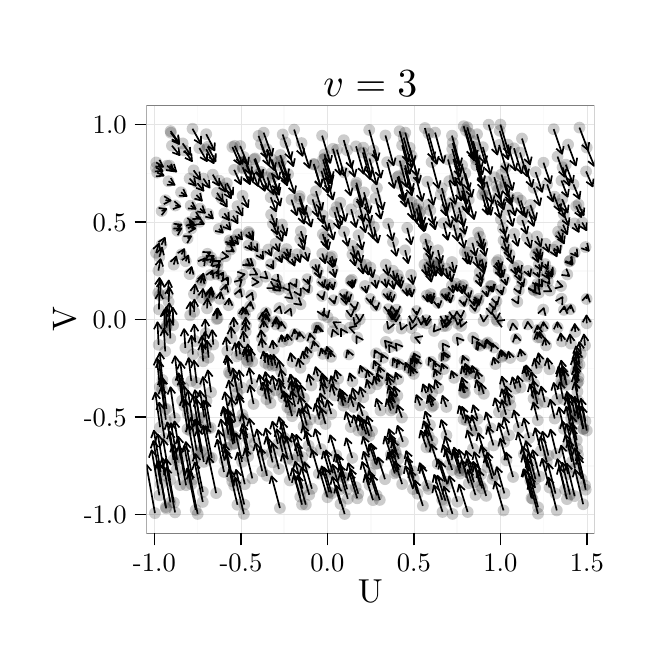
\begin{tikzpicture}[x=1pt,y=1pt]
\definecolor[named]{fillColor}{rgb}{1.00,1.00,1.00}
\path[use as bounding box,fill=fillColor,fill opacity=0.00] (0,0) rectangle (216.81,216.81);
\begin{scope}
\path[clip] (  0.00,  0.00) rectangle (216.81,216.81);
\definecolor[named]{drawColor}{rgb}{1.00,1.00,1.00}
\definecolor[named]{fillColor}{rgb}{1.00,1.00,1.00}

\path[draw=drawColor,line width= 0.6pt,line join=round,line cap=round,fill=fillColor] ( -0.00,  0.00) rectangle (216.81,216.81);
\end{scope}
\begin{scope}
\path[clip] ( 42.89, 34.03) rectangle (204.76,188.82);
\definecolor[named]{fillColor}{rgb}{1.00,1.00,1.00}

\path[fill=fillColor] ( 42.89, 34.03) rectangle (204.76,188.82);
\definecolor[named]{drawColor}{rgb}{0.98,0.98,0.98}

\path[draw=drawColor,line width= 0.6pt,line join=round] ( 42.89, 58.46) --
	(204.76, 58.46);

\path[draw=drawColor,line width= 0.6pt,line join=round] ( 42.89, 93.70) --
	(204.76, 93.70);

\path[draw=drawColor,line width= 0.6pt,line join=round] ( 42.89,128.93) --
	(204.76,128.93);

\path[draw=drawColor,line width= 0.6pt,line join=round] ( 42.89,164.17) --
	(204.76,164.17);

\path[draw=drawColor,line width= 0.6pt,line join=round] ( 61.42, 34.03) --
	( 61.42,188.82);

\path[draw=drawColor,line width= 0.6pt,line join=round] ( 92.68, 34.03) --
	( 92.68,188.82);

\path[draw=drawColor,line width= 0.6pt,line join=round] (123.94, 34.03) --
	(123.94,188.82);

\path[draw=drawColor,line width= 0.6pt,line join=round] (155.19, 34.03) --
	(155.19,188.82);

\path[draw=drawColor,line width= 0.6pt,line join=round] (186.45, 34.03) --
	(186.45,188.82);
\definecolor[named]{drawColor}{rgb}{0.90,0.90,0.90}

\path[draw=drawColor,line width= 0.2pt,line join=round] ( 42.89, 40.84) --
	(204.76, 40.84);

\path[draw=drawColor,line width= 0.2pt,line join=round] ( 42.89, 76.08) --
	(204.76, 76.08);

\path[draw=drawColor,line width= 0.2pt,line join=round] ( 42.89,111.31) --
	(204.76,111.31);

\path[draw=drawColor,line width= 0.2pt,line join=round] ( 42.89,146.55) --
	(204.76,146.55);

\path[draw=drawColor,line width= 0.2pt,line join=round] ( 42.89,181.79) --
	(204.76,181.79);

\path[draw=drawColor,line width= 0.2pt,line join=round] ( 45.79, 34.03) --
	( 45.79,188.82);

\path[draw=drawColor,line width= 0.2pt,line join=round] ( 77.05, 34.03) --
	( 77.05,188.82);

\path[draw=drawColor,line width= 0.2pt,line join=round] (108.31, 34.03) --
	(108.31,188.82);

\path[draw=drawColor,line width= 0.2pt,line join=round] (139.56, 34.03) --
	(139.56,188.82);

\path[draw=drawColor,line width= 0.2pt,line join=round] (170.82, 34.03) --
	(170.82,188.82);

\path[draw=drawColor,line width= 0.2pt,line join=round] (202.08, 34.03) --
	(202.08,188.82);
\definecolor[named]{fillColor}{rgb}{0.00,0.00,0.00}

\path[fill=fillColor,fill opacity=0.20] (170.82,181.79) circle (  2.13);

\path[fill=fillColor,fill opacity=0.20] (163.42,141.31) circle (  2.13);

\path[fill=fillColor,fill opacity=0.20] (100.70,150.30) circle (  2.13);

\path[fill=fillColor,fill opacity=0.20] (182.34, 58.73) circle (  2.13);

\path[fill=fillColor,fill opacity=0.20] (144.42,161.17) circle (  2.13);

\path[fill=fillColor,fill opacity=0.20] ( 56.01,174.98) circle (  2.13);

\path[fill=fillColor,fill opacity=0.20] (114.01, 82.13) circle (  2.13);

\path[fill=fillColor,fill opacity=0.20] (195.96, 48.11) circle (  2.13);

\path[fill=fillColor,fill opacity=0.20] (149.91, 41.81) circle (  2.13);

\path[fill=fillColor,fill opacity=0.20] ( 95.64, 96.02) circle (  2.13);

\path[fill=fillColor,fill opacity=0.20] ( 93.54,136.81) circle (  2.13);

\path[fill=fillColor,fill opacity=0.20] ( 99.36, 50.24) circle (  2.13);

\path[fill=fillColor,fill opacity=0.20] ( 71.15, 60.39) circle (  2.13);

\path[fill=fillColor,fill opacity=0.20] ( 65.65, 61.47) circle (  2.13);

\path[fill=fillColor,fill opacity=0.20] (184.05,141.42) circle (  2.13);

\path[fill=fillColor,fill opacity=0.20] (146.63,131.17) circle (  2.13);

\path[fill=fillColor,fill opacity=0.20] (167.61,123.41) circle (  2.13);

\path[fill=fillColor,fill opacity=0.20] ( 80.06,142.46) circle (  2.13);

\path[fill=fillColor,fill opacity=0.20] (130.88, 89.51) circle (  2.13);

\path[fill=fillColor,fill opacity=0.20] ( 98.97,175.11) circle (  2.13);

\path[fill=fillColor,fill opacity=0.20] (133.30, 56.26) circle (  2.13);

\path[fill=fillColor,fill opacity=0.20] (160.86, 56.03) circle (  2.13);

\path[fill=fillColor,fill opacity=0.20] ( 84.92,101.19) circle (  2.13);

\path[fill=fillColor,fill opacity=0.20] ( 96.13, 83.83) circle (  2.13);

\path[fill=fillColor,fill opacity=0.20] (146.27, 67.40) circle (  2.13);

\path[fill=fillColor,fill opacity=0.20] ( 56.58, 80.17) circle (  2.13);

\path[fill=fillColor,fill opacity=0.20] (190.06,136.56) circle (  2.13);

\path[fill=fillColor,fill opacity=0.20] ( 48.69, 89.53) circle (  2.13);

\path[fill=fillColor,fill opacity=0.20] ( 88.56,162.66) circle (  2.13);

\path[fill=fillColor,fill opacity=0.20] (156.64,109.01) circle (  2.13);

\path[fill=fillColor,fill opacity=0.20] (168.53, 54.96) circle (  2.13);

\path[fill=fillColor,fill opacity=0.20] ( 72.57, 69.74) circle (  2.13);

\path[fill=fillColor,fill opacity=0.20] ( 50.36,166.95) circle (  2.13);

\path[fill=fillColor,fill opacity=0.20] (129.28,177.85) circle (  2.13);

\path[fill=fillColor,fill opacity=0.20] ( 54.23, 89.07) circle (  2.13);

\path[fill=fillColor,fill opacity=0.20] ( 84.97, 62.47) circle (  2.13);

\path[fill=fillColor,fill opacity=0.20] ( 53.26, 41.66) circle (  2.13);

\path[fill=fillColor,fill opacity=0.20] (153.41,172.96) circle (  2.13);

\path[fill=fillColor,fill opacity=0.20] (187.52,127.49) circle (  2.13);

\path[fill=fillColor,fill opacity=0.20] ( 65.25,149.47) circle (  2.13);

\path[fill=fillColor,fill opacity=0.20] (109.62, 97.86) circle (  2.13);

\path[fill=fillColor,fill opacity=0.20] ( 80.12, 98.07) circle (  2.13);

\path[fill=fillColor,fill opacity=0.20] ( 49.93, 75.15) circle (  2.13);

\path[fill=fillColor,fill opacity=0.20] (151.09,151.51) circle (  2.13);

\path[fill=fillColor,fill opacity=0.20] (144.59,138.06) circle (  2.13);

\path[fill=fillColor,fill opacity=0.20] (191.68,143.12) circle (  2.13);

\path[fill=fillColor,fill opacity=0.20] (133.11, 62.65) circle (  2.13);

\path[fill=fillColor,fill opacity=0.20] (168.86,154.63) circle (  2.13);

\path[fill=fillColor,fill opacity=0.20] (114.35,164.51) circle (  2.13);

\path[fill=fillColor,fill opacity=0.20] (194.98,127.65) circle (  2.13);

\path[fill=fillColor,fill opacity=0.20] (200.73, 44.60) circle (  2.13);

\path[fill=fillColor,fill opacity=0.20] (170.30, 77.90) circle (  2.13);

\path[fill=fillColor,fill opacity=0.20] (138.76,170.48) circle (  2.13);

\path[fill=fillColor,fill opacity=0.20] (163.64, 51.28) circle (  2.13);

\path[fill=fillColor,fill opacity=0.20] ( 86.47, 54.89) circle (  2.13);

\path[fill=fillColor,fill opacity=0.20] (107.34,169.59) circle (  2.13);

\path[fill=fillColor,fill opacity=0.20] (169.47,159.62) circle (  2.13);

\path[fill=fillColor,fill opacity=0.20] ( 85.86, 95.71) circle (  2.13);

\path[fill=fillColor,fill opacity=0.20] ( 64.35,106.39) circle (  2.13);

\path[fill=fillColor,fill opacity=0.20] (172.88, 76.95) circle (  2.13);

\path[fill=fillColor,fill opacity=0.20] (110.53,110.33) circle (  2.13);

\path[fill=fillColor,fill opacity=0.20] ( 52.77,131.20) circle (  2.13);

\path[fill=fillColor,fill opacity=0.20] ( 55.25, 61.54) circle (  2.13);

\path[fill=fillColor,fill opacity=0.20] (151.11,129.78) circle (  2.13);

\path[fill=fillColor,fill opacity=0.20] ( 59.20, 51.85) circle (  2.13);

\path[fill=fillColor,fill opacity=0.20] (158.33,179.67) circle (  2.13);

\path[fill=fillColor,fill opacity=0.20] (202.04, 71.22) circle (  2.13);

\path[fill=fillColor,fill opacity=0.20] (106.62, 98.94) circle (  2.13);

\path[fill=fillColor,fill opacity=0.20] (129.00,126.06) circle (  2.13);

\path[fill=fillColor,fill opacity=0.20] (146.58, 80.29) circle (  2.13);

\path[fill=fillColor,fill opacity=0.20] (161.86,134.00) circle (  2.13);

\path[fill=fillColor,fill opacity=0.20] ( 54.03,144.99) circle (  2.13);

\path[fill=fillColor,fill opacity=0.20] ( 48.37,138.34) circle (  2.13);

\path[fill=fillColor,fill opacity=0.20] (159.73, 91.68) circle (  2.13);

\path[fill=fillColor,fill opacity=0.20] (153.58,175.18) circle (  2.13);

\path[fill=fillColor,fill opacity=0.20] (192.90,118.86) circle (  2.13);

\path[fill=fillColor,fill opacity=0.20] (197.87,106.88) circle (  2.13);

\path[fill=fillColor,fill opacity=0.20] (155.39,104.40) circle (  2.13);

\path[fill=fillColor,fill opacity=0.20] (131.23, 62.55) circle (  2.13);

\path[fill=fillColor,fill opacity=0.20] (117.36,137.98) circle (  2.13);

\path[fill=fillColor,fill opacity=0.20] ( 59.12,144.25) circle (  2.13);

\path[fill=fillColor,fill opacity=0.20] (180.38, 90.71) circle (  2.13);

\path[fill=fillColor,fill opacity=0.20] (114.11, 80.21) circle (  2.13);

\path[fill=fillColor,fill opacity=0.20] (107.64, 73.59) circle (  2.13);

\path[fill=fillColor,fill opacity=0.20] (132.75, 95.81) circle (  2.13);

\path[fill=fillColor,fill opacity=0.20] ( 94.10,163.88) circle (  2.13);

\path[fill=fillColor,fill opacity=0.20] (160.99,104.77) circle (  2.13);

\path[fill=fillColor,fill opacity=0.20] (161.46, 92.14) circle (  2.13);

\path[fill=fillColor,fill opacity=0.20] ( 73.42,139.28) circle (  2.13);

\path[fill=fillColor,fill opacity=0.20] ( 98.57, 93.90) circle (  2.13);

\path[fill=fillColor,fill opacity=0.20] ( 79.81,143.01) circle (  2.13);

\path[fill=fillColor,fill opacity=0.20] (114.55, 54.22) circle (  2.13);

\path[fill=fillColor,fill opacity=0.20] ( 47.20,121.01) circle (  2.13);

\path[fill=fillColor,fill opacity=0.20] (139.17, 95.67) circle (  2.13);

\path[fill=fillColor,fill opacity=0.20] (192.79, 89.31) circle (  2.13);

\path[fill=fillColor,fill opacity=0.20] (113.70, 54.44) circle (  2.13);

\path[fill=fillColor,fill opacity=0.20] ( 85.34,108.60) circle (  2.13);

\path[fill=fillColor,fill opacity=0.20] (102.70, 50.22) circle (  2.13);

\path[fill=fillColor,fill opacity=0.20] ( 64.61, 81.97) circle (  2.13);

\path[fill=fillColor,fill opacity=0.20] (157.60, 84.90) circle (  2.13);

\path[fill=fillColor,fill opacity=0.20] (164.84, 84.51) circle (  2.13);

\path[fill=fillColor,fill opacity=0.20] ( 49.80,154.44) circle (  2.13);

\path[fill=fillColor,fill opacity=0.20] (194.72, 87.69) circle (  2.13);

\path[fill=fillColor,fill opacity=0.20] ( 98.22,120.71) circle (  2.13);

\path[fill=fillColor,fill opacity=0.20] ( 91.15, 43.25) circle (  2.13);

\path[fill=fillColor,fill opacity=0.20] ( 57.11,132.40) circle (  2.13);

\path[fill=fillColor,fill opacity=0.20] (106.73,169.17) circle (  2.13);

\path[fill=fillColor,fill opacity=0.20] ( 96.62,106.19) circle (  2.13);

\path[fill=fillColor,fill opacity=0.20] (152.43,119.45) circle (  2.13);

\path[fill=fillColor,fill opacity=0.20] (145.36, 73.22) circle (  2.13);

\path[fill=fillColor,fill opacity=0.20] (173.47,150.97) circle (  2.13);

\path[fill=fillColor,fill opacity=0.20] (185.46, 63.93) circle (  2.13);

\path[fill=fillColor,fill opacity=0.20] (134.38,179.41) circle (  2.13);

\path[fill=fillColor,fill opacity=0.20] ( 86.94,136.64) circle (  2.13);

\path[fill=fillColor,fill opacity=0.20] (135.31, 51.89) circle (  2.13);

\path[fill=fillColor,fill opacity=0.20] ( 96.02, 86.87) circle (  2.13);

\path[fill=fillColor,fill opacity=0.20] (104.92, 90.88) circle (  2.13);

\path[fill=fillColor,fill opacity=0.20] (168.57,115.93) circle (  2.13);

\path[fill=fillColor,fill opacity=0.20] (132.00,139.42) circle (  2.13);

\path[fill=fillColor,fill opacity=0.20] ( 69.98,127.21) circle (  2.13);

\path[fill=fillColor,fill opacity=0.20] ( 69.24,161.52) circle (  2.13);

\path[fill=fillColor,fill opacity=0.20] (157.85, 96.57) circle (  2.13);

\path[fill=fillColor,fill opacity=0.20] (144.34, 51.29) circle (  2.13);

\path[fill=fillColor,fill opacity=0.20] ( 58.91,152.51) circle (  2.13);

\path[fill=fillColor,fill opacity=0.20] (164.74,110.88) circle (  2.13);

\path[fill=fillColor,fill opacity=0.20] ( 79.71, 64.16) circle (  2.13);

\path[fill=fillColor,fill opacity=0.20] ( 65.56,119.07) circle (  2.13);

\path[fill=fillColor,fill opacity=0.20] ( 51.55,104.52) circle (  2.13);

\path[fill=fillColor,fill opacity=0.20] (148.15, 59.21) circle (  2.13);

\path[fill=fillColor,fill opacity=0.20] (167.95, 53.75) circle (  2.13);

\path[fill=fillColor,fill opacity=0.20] (144.87,152.90) circle (  2.13);

\path[fill=fillColor,fill opacity=0.20] (177.35,127.53) circle (  2.13);

\path[fill=fillColor,fill opacity=0.20] (146.04, 79.83) circle (  2.13);

\path[fill=fillColor,fill opacity=0.20] (107.60, 87.38) circle (  2.13);

\path[fill=fillColor,fill opacity=0.20] (116.40,108.40) circle (  2.13);

\path[fill=fillColor,fill opacity=0.20] (128.49, 97.54) circle (  2.13);

\path[fill=fillColor,fill opacity=0.20] (153.84,169.36) circle (  2.13);

\path[fill=fillColor,fill opacity=0.20] ( 92.13, 63.37) circle (  2.13);

\path[fill=fillColor,fill opacity=0.20] ( 79.21, 96.70) circle (  2.13);

\path[fill=fillColor,fill opacity=0.20] ( 69.09,144.07) circle (  2.13);

\path[fill=fillColor,fill opacity=0.20] ( 99.61, 58.16) circle (  2.13);

\path[fill=fillColor,fill opacity=0.20] ( 66.25, 85.08) circle (  2.13);

\path[fill=fillColor,fill opacity=0.20] (102.65, 63.43) circle (  2.13);

\path[fill=fillColor,fill opacity=0.20] (170.58,179.55) circle (  2.13);

\path[fill=fillColor,fill opacity=0.20] ( 78.55,113.25) circle (  2.13);

\path[fill=fillColor,fill opacity=0.20] (106.65,148.99) circle (  2.13);

\path[fill=fillColor,fill opacity=0.20] (156.40,148.49) circle (  2.13);

\path[fill=fillColor,fill opacity=0.20] (172.58,160.02) circle (  2.13);

\path[fill=fillColor,fill opacity=0.20] ( 63.27, 45.44) circle (  2.13);

\path[fill=fillColor,fill opacity=0.20] ( 73.72,104.59) circle (  2.13);

\path[fill=fillColor,fill opacity=0.20] ( 84.56,104.62) circle (  2.13);

\path[fill=fillColor,fill opacity=0.20] ( 56.24, 86.92) circle (  2.13);

\path[fill=fillColor,fill opacity=0.20] ( 61.43, 41.09) circle (  2.13);

\path[fill=fillColor,fill opacity=0.20] (101.05,125.93) circle (  2.13);

\path[fill=fillColor,fill opacity=0.20] (134.49,160.38) circle (  2.13);

\path[fill=fillColor,fill opacity=0.20] (154.36,162.76) circle (  2.13);

\path[fill=fillColor,fill opacity=0.20] (150.89,120.65) circle (  2.13);

\path[fill=fillColor,fill opacity=0.20] ( 68.42,157.15) circle (  2.13);

\path[fill=fillColor,fill opacity=0.20] (145.68,119.25) circle (  2.13);

\path[fill=fillColor,fill opacity=0.20] (174.14,135.04) circle (  2.13);

\path[fill=fillColor,fill opacity=0.20] ( 74.19,148.84) circle (  2.13);

\path[fill=fillColor,fill opacity=0.20] (106.36,125.01) circle (  2.13);

\path[fill=fillColor,fill opacity=0.20] (164.04,131.55) circle (  2.13);

\path[fill=fillColor,fill opacity=0.20] (197.58,146.07) circle (  2.13);

\path[fill=fillColor,fill opacity=0.20] (163.18, 89.84) circle (  2.13);

\path[fill=fillColor,fill opacity=0.20] ( 70.94, 56.27) circle (  2.13);

\path[fill=fillColor,fill opacity=0.20] (163.33,128.49) circle (  2.13);

\path[fill=fillColor,fill opacity=0.20] (107.37,141.12) circle (  2.13);

\path[fill=fillColor,fill opacity=0.20] (150.32, 97.84) circle (  2.13);

\path[fill=fillColor,fill opacity=0.20] ( 82.85,124.89) circle (  2.13);

\path[fill=fillColor,fill opacity=0.20] (133.34,114.91) circle (  2.13);

\path[fill=fillColor,fill opacity=0.20] ( 95.98, 86.94) circle (  2.13);

\path[fill=fillColor,fill opacity=0.20] ( 84.89,112.14) circle (  2.13);

\path[fill=fillColor,fill opacity=0.20] (177.48,121.92) circle (  2.13);

\path[fill=fillColor,fill opacity=0.20] (176.50,104.43) circle (  2.13);

\path[fill=fillColor,fill opacity=0.20] (139.50, 91.69) circle (  2.13);

\path[fill=fillColor,fill opacity=0.20] ( 74.55,108.65) circle (  2.13);

\path[fill=fillColor,fill opacity=0.20] (117.33, 88.98) circle (  2.13);

\path[fill=fillColor,fill opacity=0.20] ( 47.82,120.12) circle (  2.13);

\path[fill=fillColor,fill opacity=0.20] (131.01,101.46) circle (  2.13);

\path[fill=fillColor,fill opacity=0.20] ( 55.07, 51.53) circle (  2.13);

\path[fill=fillColor,fill opacity=0.20] (125.92, 99.12) circle (  2.13);

\path[fill=fillColor,fill opacity=0.20] ( 77.64,156.05) circle (  2.13);

\path[fill=fillColor,fill opacity=0.20] (174.45, 80.37) circle (  2.13);

\path[fill=fillColor,fill opacity=0.20] ( 98.49, 47.35) circle (  2.13);

\path[fill=fillColor,fill opacity=0.20] (140.88, 48.39) circle (  2.13);

\path[fill=fillColor,fill opacity=0.20] (122.22,131.20) circle (  2.13);

\path[fill=fillColor,fill opacity=0.20] (165.67,121.54) circle (  2.13);

\path[fill=fillColor,fill opacity=0.20] ( 52.13,174.15) circle (  2.13);

\path[fill=fillColor,fill opacity=0.20] (114.54, 41.07) circle (  2.13);

\path[fill=fillColor,fill opacity=0.20] ( 45.99, 41.40) circle (  2.13);

\path[fill=fillColor,fill opacity=0.20] (182.41, 46.59) circle (  2.13);

\path[fill=fillColor,fill opacity=0.20] (151.04,120.56) circle (  2.13);

\path[fill=fillColor,fill opacity=0.20] ( 64.96,135.09) circle (  2.13);

\path[fill=fillColor,fill opacity=0.20] ( 98.10,151.37) circle (  2.13);

\path[fill=fillColor,fill opacity=0.20] (131.62, 84.16) circle (  2.13);

\path[fill=fillColor,fill opacity=0.20] ( 46.38,135.45) circle (  2.13);

\path[fill=fillColor,fill opacity=0.20] ( 58.71,112.87) circle (  2.13);

\path[fill=fillColor,fill opacity=0.20] (132.52, 65.69) circle (  2.13);

\path[fill=fillColor,fill opacity=0.20] ( 57.77,140.67) circle (  2.13);

\path[fill=fillColor,fill opacity=0.20] ( 84.35,164.65) circle (  2.13);

\path[fill=fillColor,fill opacity=0.20] (114.30,143.05) circle (  2.13);

\path[fill=fillColor,fill opacity=0.20] ( 85.27,178.87) circle (  2.13);

\path[fill=fillColor,fill opacity=0.20] (195.23, 55.51) circle (  2.13);

\path[fill=fillColor,fill opacity=0.20] ( 89.84,110.77) circle (  2.13);

\path[fill=fillColor,fill opacity=0.20] (183.81,137.02) circle (  2.13);

\path[fill=fillColor,fill opacity=0.20] ( 60.14,114.15) circle (  2.13);

\path[fill=fillColor,fill opacity=0.20] (163.84, 55.36) circle (  2.13);

\path[fill=fillColor,fill opacity=0.20] ( 61.48, 73.50) circle (  2.13);

\path[fill=fillColor,fill opacity=0.20] ( 91.59, 92.53) circle (  2.13);

\path[fill=fillColor,fill opacity=0.20] ( 66.12, 72.19) circle (  2.13);

\path[fill=fillColor,fill opacity=0.20] (181.64,152.76) circle (  2.13);

\path[fill=fillColor,fill opacity=0.20] (202.00,110.00) circle (  2.13);

\path[fill=fillColor,fill opacity=0.20] (173.00, 60.50) circle (  2.13);

\path[fill=fillColor,fill opacity=0.20] ( 72.12, 99.95) circle (  2.13);

\path[fill=fillColor,fill opacity=0.20] ( 61.05, 64.00) circle (  2.13);

\path[fill=fillColor,fill opacity=0.20] ( 91.28,166.99) circle (  2.13);

\path[fill=fillColor,fill opacity=0.20] (199.02, 89.00) circle (  2.13);

\path[fill=fillColor,fill opacity=0.20] (164.88,157.92) circle (  2.13);

\path[fill=fillColor,fill opacity=0.20] ( 80.35,116.13) circle (  2.13);

\path[fill=fillColor,fill opacity=0.20] ( 90.94,115.49) circle (  2.13);

\path[fill=fillColor,fill opacity=0.20] (172.67, 81.60) circle (  2.13);

\path[fill=fillColor,fill opacity=0.20] (153.90,145.62) circle (  2.13);

\path[fill=fillColor,fill opacity=0.20] (133.59, 83.82) circle (  2.13);

\path[fill=fillColor,fill opacity=0.20] (134.43,168.75) circle (  2.13);

\path[fill=fillColor,fill opacity=0.20] ( 52.70, 60.66) circle (  2.13);

\path[fill=fillColor,fill opacity=0.20] ( 75.52, 98.02) circle (  2.13);

\path[fill=fillColor,fill opacity=0.20] (125.91, 94.57) circle (  2.13);

\path[fill=fillColor,fill opacity=0.20] (187.00,131.38) circle (  2.13);

\path[fill=fillColor,fill opacity=0.20] (153.32,177.78) circle (  2.13);

\path[fill=fillColor,fill opacity=0.20] ( 97.38,134.95) circle (  2.13);

\path[fill=fillColor,fill opacity=0.20] (134.03,163.20) circle (  2.13);

\path[fill=fillColor,fill opacity=0.20] ( 50.93,117.76) circle (  2.13);

\path[fill=fillColor,fill opacity=0.20] (110.88,150.18) circle (  2.13);

\path[fill=fillColor,fill opacity=0.20] (125.74, 59.16) circle (  2.13);

\path[fill=fillColor,fill opacity=0.20] (197.64, 47.54) circle (  2.13);

\path[fill=fillColor,fill opacity=0.20] ( 97.86, 85.52) circle (  2.13);

\path[fill=fillColor,fill opacity=0.20] ( 48.05, 56.29) circle (  2.13);

\path[fill=fillColor,fill opacity=0.20] (198.06, 92.61) circle (  2.13);

\path[fill=fillColor,fill opacity=0.20] (140.27,162.84) circle (  2.13);

\path[fill=fillColor,fill opacity=0.20] ( 62.02,173.32) circle (  2.13);

\path[fill=fillColor,fill opacity=0.20] ( 83.36,163.75) circle (  2.13);

\path[fill=fillColor,fill opacity=0.20] (137.14,144.44) circle (  2.13);

\path[fill=fillColor,fill opacity=0.20] (176.25, 86.37) circle (  2.13);

\path[fill=fillColor,fill opacity=0.20] (143.72,140.47) circle (  2.13);

\path[fill=fillColor,fill opacity=0.20] (144.01, 84.78) circle (  2.13);

\path[fill=fillColor,fill opacity=0.20] (119.57,153.68) circle (  2.13);

\path[fill=fillColor,fill opacity=0.20] (108.36,112.23) circle (  2.13);

\path[fill=fillColor,fill opacity=0.20] (106.87,112.84) circle (  2.13);

\path[fill=fillColor,fill opacity=0.20] (201.53, 74.63) circle (  2.13);

\path[fill=fillColor,fill opacity=0.20] ( 66.36,132.51) circle (  2.13);

\path[fill=fillColor,fill opacity=0.20] (175.75,142.33) circle (  2.13);

\path[fill=fillColor,fill opacity=0.20] (118.64, 82.65) circle (  2.13);

\path[fill=fillColor,fill opacity=0.20] ( 61.34,160.63) circle (  2.13);

\path[fill=fillColor,fill opacity=0.20] ( 92.43, 88.73) circle (  2.13);

\path[fill=fillColor,fill opacity=0.20] ( 53.33,152.56) circle (  2.13);

\path[fill=fillColor,fill opacity=0.20] (172.71,166.29) circle (  2.13);

\path[fill=fillColor,fill opacity=0.20] (186.30,114.94) circle (  2.13);

\path[fill=fillColor,fill opacity=0.20] (135.10,108.08) circle (  2.13);

\path[fill=fillColor,fill opacity=0.20] (166.58,181.75) circle (  2.13);

\path[fill=fillColor,fill opacity=0.20] (170.34,174.42) circle (  2.13);

\path[fill=fillColor,fill opacity=0.20] (143.37,131.18) circle (  2.13);

\path[fill=fillColor,fill opacity=0.20] (131.25, 78.47) circle (  2.13);

\path[fill=fillColor,fill opacity=0.20] (194.21, 89.45) circle (  2.13);

\path[fill=fillColor,fill opacity=0.20] ( 56.88, 55.30) circle (  2.13);

\path[fill=fillColor,fill opacity=0.20] ( 88.70,123.00) circle (  2.13);

\path[fill=fillColor,fill opacity=0.20] ( 97.69, 61.95) circle (  2.13);

\path[fill=fillColor,fill opacity=0.20] (132.20, 79.16) circle (  2.13);

\path[fill=fillColor,fill opacity=0.20] (170.21,129.23) circle (  2.13);

\path[fill=fillColor,fill opacity=0.20] ( 71.07,149.71) circle (  2.13);

\path[fill=fillColor,fill opacity=0.20] (116.78,113.10) circle (  2.13);

\path[fill=fillColor,fill opacity=0.20] (121.90,123.46) circle (  2.13);

\path[fill=fillColor,fill opacity=0.20] (150.79, 52.78) circle (  2.13);

\path[fill=fillColor,fill opacity=0.20] (183.02,121.85) circle (  2.13);

\path[fill=fillColor,fill opacity=0.20] (145.61,120.54) circle (  2.13);

\path[fill=fillColor,fill opacity=0.20] (119.99,111.35) circle (  2.13);

\path[fill=fillColor,fill opacity=0.20] ( 81.62, 80.83) circle (  2.13);

\path[fill=fillColor,fill opacity=0.20] ( 66.53, 61.38) circle (  2.13);

\path[fill=fillColor,fill opacity=0.20] (147.96, 91.11) circle (  2.13);

\path[fill=fillColor,fill opacity=0.20] ( 46.44,168.11) circle (  2.13);

\path[fill=fillColor,fill opacity=0.20] (165.82,102.58) circle (  2.13);

\path[fill=fillColor,fill opacity=0.20] ( 62.87,125.65) circle (  2.13);

\path[fill=fillColor,fill opacity=0.20] (138.05,173.42) circle (  2.13);

\path[fill=fillColor,fill opacity=0.20] (150.47,110.85) circle (  2.13);

\path[fill=fillColor,fill opacity=0.20] ( 98.16,155.03) circle (  2.13);

\path[fill=fillColor,fill opacity=0.20] (186.38,168.01) circle (  2.13);

\path[fill=fillColor,fill opacity=0.20] ( 62.49,124.47) circle (  2.13);

\path[fill=fillColor,fill opacity=0.20] (103.40,167.35) circle (  2.13);

\path[fill=fillColor,fill opacity=0.20] (187.08,138.76) circle (  2.13);

\path[fill=fillColor,fill opacity=0.20] (166.19, 57.94) circle (  2.13);

\path[fill=fillColor,fill opacity=0.20] ( 52.85, 45.20) circle (  2.13);

\path[fill=fillColor,fill opacity=0.20] (112.88, 49.98) circle (  2.13);

\path[fill=fillColor,fill opacity=0.20] ( 94.74, 53.19) circle (  2.13);

\path[fill=fillColor,fill opacity=0.20] (121.52,157.30) circle (  2.13);

\path[fill=fillColor,fill opacity=0.20] (154.73,124.29) circle (  2.13);

\path[fill=fillColor,fill opacity=0.20] ( 49.42, 68.44) circle (  2.13);

\path[fill=fillColor,fill opacity=0.20] ( 82.22,128.00) circle (  2.13);

\path[fill=fillColor,fill opacity=0.20] (193.74,149.36) circle (  2.13);

\path[fill=fillColor,fill opacity=0.20] (187.96,125.10) circle (  2.13);

\path[fill=fillColor,fill opacity=0.20] (140.54,151.43) circle (  2.13);

\path[fill=fillColor,fill opacity=0.20] ( 91.01,123.24) circle (  2.13);

\path[fill=fillColor,fill opacity=0.20] (109.25,133.75) circle (  2.13);

\path[fill=fillColor,fill opacity=0.20] (141.86, 80.28) circle (  2.13);

\path[fill=fillColor,fill opacity=0.20] (131.68,112.42) circle (  2.13);

\path[fill=fillColor,fill opacity=0.20] ( 78.99,167.39) circle (  2.13);

\path[fill=fillColor,fill opacity=0.20] (105.05,108.42) circle (  2.13);

\path[fill=fillColor,fill opacity=0.20] (157.23,157.00) circle (  2.13);

\path[fill=fillColor,fill opacity=0.20] (157.96,135.87) circle (  2.13);

\path[fill=fillColor,fill opacity=0.20] (106.65,142.19) circle (  2.13);

\path[fill=fillColor,fill opacity=0.20] (184.32,104.86) circle (  2.13);

\path[fill=fillColor,fill opacity=0.20] (150.41, 93.45) circle (  2.13);

\path[fill=fillColor,fill opacity=0.20] (113.04, 44.70) circle (  2.13);

\path[fill=fillColor,fill opacity=0.20] (100.02, 97.08) circle (  2.13);

\path[fill=fillColor,fill opacity=0.20] (162.24, 71.09) circle (  2.13);

\path[fill=fillColor,fill opacity=0.20] (198.56, 94.87) circle (  2.13);

\path[fill=fillColor,fill opacity=0.20] (184.24,124.26) circle (  2.13);

\path[fill=fillColor,fill opacity=0.20] (185.23, 95.82) circle (  2.13);

\path[fill=fillColor,fill opacity=0.20] (144.09, 65.15) circle (  2.13);

\path[fill=fillColor,fill opacity=0.20] ( 79.66, 61.87) circle (  2.13);

\path[fill=fillColor,fill opacity=0.20] ( 79.55,131.44) circle (  2.13);

\path[fill=fillColor,fill opacity=0.20] (108.00,162.37) circle (  2.13);

\path[fill=fillColor,fill opacity=0.20] (196.35, 71.95) circle (  2.13);

\path[fill=fillColor,fill opacity=0.20] ( 75.03, 74.42) circle (  2.13);

\path[fill=fillColor,fill opacity=0.20] (116.76, 72.49) circle (  2.13);

\path[fill=fillColor,fill opacity=0.20] ( 68.65,111.78) circle (  2.13);

\path[fill=fillColor,fill opacity=0.20] ( 76.08,142.17) circle (  2.13);

\path[fill=fillColor,fill opacity=0.20] ( 63.30, 49.05) circle (  2.13);

\path[fill=fillColor,fill opacity=0.20] (190.38,155.74) circle (  2.13);

\path[fill=fillColor,fill opacity=0.20] ( 65.39, 97.55) circle (  2.13);

\path[fill=fillColor,fill opacity=0.20] (159.39,154.68) circle (  2.13);

\path[fill=fillColor,fill opacity=0.20] ( 75.25, 87.17) circle (  2.13);

\path[fill=fillColor,fill opacity=0.20] (104.42,108.44) circle (  2.13);

\path[fill=fillColor,fill opacity=0.20] (190.74, 48.46) circle (  2.13);

\path[fill=fillColor,fill opacity=0.20] (167.25,123.47) circle (  2.13);

\path[fill=fillColor,fill opacity=0.20] ( 50.15, 79.06) circle (  2.13);

\path[fill=fillColor,fill opacity=0.20] ( 77.59, 76.97) circle (  2.13);

\path[fill=fillColor,fill opacity=0.20] ( 49.51, 54.95) circle (  2.13);

\path[fill=fillColor,fill opacity=0.20] ( 99.80, 77.93) circle (  2.13);

\path[fill=fillColor,fill opacity=0.20] (192.94,103.44) circle (  2.13);

\path[fill=fillColor,fill opacity=0.20] (187.69,160.17) circle (  2.13);

\path[fill=fillColor,fill opacity=0.20] ( 59.97,165.25) circle (  2.13);

\path[fill=fillColor,fill opacity=0.20] ( 65.26, 72.05) circle (  2.13);

\path[fill=fillColor,fill opacity=0.20] ( 82.18,169.56) circle (  2.13);

\path[fill=fillColor,fill opacity=0.20] ( 77.88,165.91) circle (  2.13);

\path[fill=fillColor,fill opacity=0.20] (119.51, 71.20) circle (  2.13);

\path[fill=fillColor,fill opacity=0.20] ( 98.71,143.24) circle (  2.13);

\path[fill=fillColor,fill opacity=0.20] (171.00,147.53) circle (  2.13);

\path[fill=fillColor,fill opacity=0.20] ( 49.53, 78.98) circle (  2.13);

\path[fill=fillColor,fill opacity=0.20] (101.74, 48.02) circle (  2.13);

\path[fill=fillColor,fill opacity=0.20] (106.37,119.87) circle (  2.13);

\path[fill=fillColor,fill opacity=0.20] ( 70.04,155.20) circle (  2.13);

\path[fill=fillColor,fill opacity=0.20] ( 94.11,103.87) circle (  2.13);

\path[fill=fillColor,fill opacity=0.20] ( 58.51,127.76) circle (  2.13);

\path[fill=fillColor,fill opacity=0.20] (152.38, 58.90) circle (  2.13);

\path[fill=fillColor,fill opacity=0.20] (199.05, 90.51) circle (  2.13);

\path[fill=fillColor,fill opacity=0.20] (120.35,131.58) circle (  2.13);

\path[fill=fillColor,fill opacity=0.20] (190.43, 75.57) circle (  2.13);

\path[fill=fillColor,fill opacity=0.20] (195.21, 65.83) circle (  2.13);

\path[fill=fillColor,fill opacity=0.20] (137.32,155.14) circle (  2.13);

\path[fill=fillColor,fill opacity=0.20] (184.68,120.99) circle (  2.13);

\path[fill=fillColor,fill opacity=0.20] (129.89,120.78) circle (  2.13);

\path[fill=fillColor,fill opacity=0.20] (158.99, 41.80) circle (  2.13);

\path[fill=fillColor,fill opacity=0.20] (157.92, 87.24) circle (  2.13);

\path[fill=fillColor,fill opacity=0.20] (118.55, 50.81) circle (  2.13);

\path[fill=fillColor,fill opacity=0.20] (116.70,125.28) circle (  2.13);

\path[fill=fillColor,fill opacity=0.20] (146.58,130.99) circle (  2.13);

\path[fill=fillColor,fill opacity=0.20] ( 98.50,140.41) circle (  2.13);

\path[fill=fillColor,fill opacity=0.20] (160.68,139.06) circle (  2.13);

\path[fill=fillColor,fill opacity=0.20] (135.88,177.08) circle (  2.13);

\path[fill=fillColor,fill opacity=0.20] ( 62.09,146.66) circle (  2.13);

\path[fill=fillColor,fill opacity=0.20] (113.38,107.66) circle (  2.13);

\path[fill=fillColor,fill opacity=0.20] (171.96,140.00) circle (  2.13);

\path[fill=fillColor,fill opacity=0.20] (123.40, 62.26) circle (  2.13);

\path[fill=fillColor,fill opacity=0.20] (154.07, 90.26) circle (  2.13);

\path[fill=fillColor,fill opacity=0.20] (181.21, 68.52) circle (  2.13);

\path[fill=fillColor,fill opacity=0.20] (161.52,115.55) circle (  2.13);

\path[fill=fillColor,fill opacity=0.20] (201.40,101.97) circle (  2.13);

\path[fill=fillColor,fill opacity=0.20] (193.53, 82.62) circle (  2.13);

\path[fill=fillColor,fill opacity=0.20] (163.28, 86.03) circle (  2.13);

\path[fill=fillColor,fill opacity=0.20] ( 71.97,160.60) circle (  2.13);

\path[fill=fillColor,fill opacity=0.20] (121.31, 83.26) circle (  2.13);

\path[fill=fillColor,fill opacity=0.20] ( 77.72,113.56) circle (  2.13);

\path[fill=fillColor,fill opacity=0.20] (145.50,150.77) circle (  2.13);

\path[fill=fillColor,fill opacity=0.20] ( 67.07,102.30) circle (  2.13);

\path[fill=fillColor,fill opacity=0.20] (171.57, 98.30) circle (  2.13);

\path[fill=fillColor,fill opacity=0.20] (108.99, 48.98) circle (  2.13);

\path[fill=fillColor,fill opacity=0.20] ( 76.78,174.05) circle (  2.13);

\path[fill=fillColor,fill opacity=0.20] (123.85,130.17) circle (  2.13);

\path[fill=fillColor,fill opacity=0.20] (123.53, 51.54) circle (  2.13);

\path[fill=fillColor,fill opacity=0.20] ( 81.17, 53.96) circle (  2.13);

\path[fill=fillColor,fill opacity=0.20] (106.91,165.97) circle (  2.13);

\path[fill=fillColor,fill opacity=0.20] (168.59,162.78) circle (  2.13);

\path[fill=fillColor,fill opacity=0.20] (156.96,167.08) circle (  2.13);

\path[fill=fillColor,fill opacity=0.20] (109.72, 77.20) circle (  2.13);

\path[fill=fillColor,fill opacity=0.20] (142.23,110.22) circle (  2.13);

\path[fill=fillColor,fill opacity=0.20] (194.86, 46.45) circle (  2.13);

\path[fill=fillColor,fill opacity=0.20] (139.70, 96.79) circle (  2.13);

\path[fill=fillColor,fill opacity=0.20] ( 59.69, 53.53) circle (  2.13);

\path[fill=fillColor,fill opacity=0.20] ( 78.77,106.94) circle (  2.13);

\path[fill=fillColor,fill opacity=0.20] (110.55,118.29) circle (  2.13);

\path[fill=fillColor,fill opacity=0.20] ( 68.24,127.67) circle (  2.13);

\path[fill=fillColor,fill opacity=0.20] (131.98,128.98) circle (  2.13);

\path[fill=fillColor,fill opacity=0.20] (147.22,178.90) circle (  2.13);

\path[fill=fillColor,fill opacity=0.20] (175.72,173.21) circle (  2.13);

\path[fill=fillColor,fill opacity=0.20] (134.12, 56.98) circle (  2.13);

\path[fill=fillColor,fill opacity=0.20] ( 88.53, 59.73) circle (  2.13);

\path[fill=fillColor,fill opacity=0.20] ( 85.91,111.34) circle (  2.13);

\path[fill=fillColor,fill opacity=0.20] (153.82,112.71) circle (  2.13);

\path[fill=fillColor,fill opacity=0.20] (125.81,116.31) circle (  2.13);

\path[fill=fillColor,fill opacity=0.20] ( 94.16,122.45) circle (  2.13);

\path[fill=fillColor,fill opacity=0.20] ( 52.55,109.33) circle (  2.13);

\path[fill=fillColor,fill opacity=0.20] ( 69.40,118.81) circle (  2.13);

\path[fill=fillColor,fill opacity=0.20] (133.88, 89.74) circle (  2.13);

\path[fill=fillColor,fill opacity=0.20] (159.17,121.14) circle (  2.13);

\path[fill=fillColor,fill opacity=0.20] (165.37,156.19) circle (  2.13);

\path[fill=fillColor,fill opacity=0.20] ( 91.76,108.93) circle (  2.13);

\path[fill=fillColor,fill opacity=0.20] ( 76.78, 98.80) circle (  2.13);

\path[fill=fillColor,fill opacity=0.20] ( 50.04, 43.11) circle (  2.13);

\path[fill=fillColor,fill opacity=0.20] (117.16,125.75) circle (  2.13);

\path[fill=fillColor,fill opacity=0.20] (142.81, 44.03) circle (  2.13);

\path[fill=fillColor,fill opacity=0.20] (115.81,119.51) circle (  2.13);

\path[fill=fillColor,fill opacity=0.20] (188.95,128.86) circle (  2.13);

\path[fill=fillColor,fill opacity=0.20] ( 83.42,177.73) circle (  2.13);

\path[fill=fillColor,fill opacity=0.20] (108.95,145.48) circle (  2.13);

\path[fill=fillColor,fill opacity=0.20] ( 88.16,164.29) circle (  2.13);

\path[fill=fillColor,fill opacity=0.20] ( 78.09,170.09) circle (  2.13);

\path[fill=fillColor,fill opacity=0.20] ( 51.57, 45.25) circle (  2.13);

\path[fill=fillColor,fill opacity=0.20] (161.09,117.96) circle (  2.13);

\path[fill=fillColor,fill opacity=0.20] (198.96, 81.91) circle (  2.13);

\path[fill=fillColor,fill opacity=0.20] (160.44, 71.18) circle (  2.13);

\path[fill=fillColor,fill opacity=0.20] ( 80.54,131.61) circle (  2.13);

\path[fill=fillColor,fill opacity=0.20] ( 60.68,148.63) circle (  2.13);

\path[fill=fillColor,fill opacity=0.20] ( 77.45, 59.90) circle (  2.13);

\path[fill=fillColor,fill opacity=0.20] (184.25, 80.80) circle (  2.13);

\path[fill=fillColor,fill opacity=0.20] (125.11,144.83) circle (  2.13);

\path[fill=fillColor,fill opacity=0.20] (120.37,149.18) circle (  2.13);

\path[fill=fillColor,fill opacity=0.20] (118.30,109.59) circle (  2.13);

\path[fill=fillColor,fill opacity=0.20] (195.97,132.61) circle (  2.13);

\path[fill=fillColor,fill opacity=0.20] ( 74.79,140.04) circle (  2.13);

\path[fill=fillColor,fill opacity=0.20] ( 76.72,125.11) circle (  2.13);

\path[fill=fillColor,fill opacity=0.20] (105.22, 55.65) circle (  2.13);

\path[fill=fillColor,fill opacity=0.20] (123.83, 55.89) circle (  2.13);

\path[fill=fillColor,fill opacity=0.20] (202.01,173.49) circle (  2.13);

\path[fill=fillColor,fill opacity=0.20] (126.17, 87.93) circle (  2.13);

\path[fill=fillColor,fill opacity=0.20] ( 79.55, 95.88) circle (  2.13);

\path[fill=fillColor,fill opacity=0.20] ( 62.61, 63.49) circle (  2.13);

\path[fill=fillColor,fill opacity=0.20] ( 81.15, 96.15) circle (  2.13);

\path[fill=fillColor,fill opacity=0.20] ( 95.45,133.26) circle (  2.13);

\path[fill=fillColor,fill opacity=0.20] (115.69, 46.58) circle (  2.13);

\path[fill=fillColor,fill opacity=0.20] ( 88.19,169.16) circle (  2.13);

\path[fill=fillColor,fill opacity=0.20] (139.16,111.04) circle (  2.13);

\path[fill=fillColor,fill opacity=0.20] ( 54.02, 60.60) circle (  2.13);

\path[fill=fillColor,fill opacity=0.20] (107.27,171.02) circle (  2.13);

\path[fill=fillColor,fill opacity=0.20] ( 89.17,158.15) circle (  2.13);

\path[fill=fillColor,fill opacity=0.20] (146.85,107.22) circle (  2.13);

\path[fill=fillColor,fill opacity=0.20] (117.29, 61.35) circle (  2.13);

\path[fill=fillColor,fill opacity=0.20] (135.30,174.32) circle (  2.13);

\path[fill=fillColor,fill opacity=0.20] ( 74.81, 66.62) circle (  2.13);

\path[fill=fillColor,fill opacity=0.20] (177.88,171.68) circle (  2.13);

\path[fill=fillColor,fill opacity=0.20] (179.74,167.08) circle (  2.13);

\path[fill=fillColor,fill opacity=0.20] ( 98.10, 83.50) circle (  2.13);

\path[fill=fillColor,fill opacity=0.20] (132.21, 81.57) circle (  2.13);

\path[fill=fillColor,fill opacity=0.20] ( 90.76,122.16) circle (  2.13);

\path[fill=fillColor,fill opacity=0.20] (162.74,118.01) circle (  2.13);

\path[fill=fillColor,fill opacity=0.20] (144.91,134.20) circle (  2.13);

\path[fill=fillColor,fill opacity=0.20] (125.70,155.13) circle (  2.13);

\path[fill=fillColor,fill opacity=0.20] (178.20,154.36) circle (  2.13);

\path[fill=fillColor,fill opacity=0.20] (145.95,168.26) circle (  2.13);

\path[fill=fillColor,fill opacity=0.20] ( 56.67,172.42) circle (  2.13);

\path[fill=fillColor,fill opacity=0.20] (198.65, 85.27) circle (  2.13);

\path[fill=fillColor,fill opacity=0.20] (195.81,132.32) circle (  2.13);

\path[fill=fillColor,fill opacity=0.20] (172.48,161.06) circle (  2.13);

\path[fill=fillColor,fill opacity=0.20] ( 71.72,125.44) circle (  2.13);

\path[fill=fillColor,fill opacity=0.20] (138.74, 92.80) circle (  2.13);

\path[fill=fillColor,fill opacity=0.20] (140.31,104.73) circle (  2.13);

\path[fill=fillColor,fill opacity=0.20] (114.30,120.38) circle (  2.13);

\path[fill=fillColor,fill opacity=0.20] (175.40, 54.46) circle (  2.13);

\path[fill=fillColor,fill opacity=0.20] (118.65,173.92) circle (  2.13);

\path[fill=fillColor,fill opacity=0.20] ( 73.17, 91.66) circle (  2.13);

\path[fill=fillColor,fill opacity=0.20] (144.87, 50.10) circle (  2.13);

\path[fill=fillColor,fill opacity=0.20] (182.89,158.95) circle (  2.13);

\path[fill=fillColor,fill opacity=0.20] ( 77.70,166.36) circle (  2.13);

\path[fill=fillColor,fill opacity=0.20] (121.02, 92.34) circle (  2.13);

\path[fill=fillColor,fill opacity=0.20] ( 57.90, 77.11) circle (  2.13);

\path[fill=fillColor,fill opacity=0.20] (162.13,166.97) circle (  2.13);

\path[fill=fillColor,fill opacity=0.20] (115.42,172.52) circle (  2.13);

\path[fill=fillColor,fill opacity=0.20] ( 49.51,107.86) circle (  2.13);

\path[fill=fillColor,fill opacity=0.20] ( 89.69,109.59) circle (  2.13);

\path[fill=fillColor,fill opacity=0.20] ( 58.72, 71.19) circle (  2.13);

\path[fill=fillColor,fill opacity=0.20] ( 59.03,145.65) circle (  2.13);

\path[fill=fillColor,fill opacity=0.20] (177.22,130.76) circle (  2.13);

\path[fill=fillColor,fill opacity=0.20] ( 71.47,134.21) circle (  2.13);

\path[fill=fillColor,fill opacity=0.20] (184.11,128.38) circle (  2.13);

\path[fill=fillColor,fill opacity=0.20] ( 58.36,146.52) circle (  2.13);

\path[fill=fillColor,fill opacity=0.20] ( 60.50,103.58) circle (  2.13);

\path[fill=fillColor,fill opacity=0.20] (145.61, 65.20) circle (  2.13);

\path[fill=fillColor,fill opacity=0.20] ( 63.02,119.15) circle (  2.13);

\path[fill=fillColor,fill opacity=0.20] (156.58,161.47) circle (  2.13);

\path[fill=fillColor,fill opacity=0.20] (141.87,150.29) circle (  2.13);

\path[fill=fillColor,fill opacity=0.20] (140.11, 97.97) circle (  2.13);

\path[fill=fillColor,fill opacity=0.20] (148.24,136.39) circle (  2.13);

\path[fill=fillColor,fill opacity=0.20] ( 66.88,163.70) circle (  2.13);

\path[fill=fillColor,fill opacity=0.20] (102.19, 75.24) circle (  2.13);

\path[fill=fillColor,fill opacity=0.20] (102.53, 87.51) circle (  2.13);

\path[fill=fillColor,fill opacity=0.20] ( 71.75,145.70) circle (  2.13);

\path[fill=fillColor,fill opacity=0.20] (112.16, 89.94) circle (  2.13);

\path[fill=fillColor,fill opacity=0.20] ( 46.35,166.27) circle (  2.13);

\path[fill=fillColor,fill opacity=0.20] ( 58.51,162.29) circle (  2.13);

\path[fill=fillColor,fill opacity=0.20] (158.12,164.18) circle (  2.13);

\path[fill=fillColor,fill opacity=0.20] ( 93.01,135.28) circle (  2.13);

\path[fill=fillColor,fill opacity=0.20] ( 73.98, 69.50) circle (  2.13);

\path[fill=fillColor,fill opacity=0.20] ( 84.30,174.74) circle (  2.13);

\path[fill=fillColor,fill opacity=0.20] ( 57.73, 71.75) circle (  2.13);

\path[fill=fillColor,fill opacity=0.20] ( 93.81, 79.66) circle (  2.13);

\path[fill=fillColor,fill opacity=0.20] (123.64, 86.43) circle (  2.13);

\path[fill=fillColor,fill opacity=0.20] (147.57, 94.23) circle (  2.13);

\path[fill=fillColor,fill opacity=0.20] ( 74.83,174.10) circle (  2.13);

\path[fill=fillColor,fill opacity=0.20] ( 89.56, 94.77) circle (  2.13);

\path[fill=fillColor,fill opacity=0.20] (118.76,160.79) circle (  2.13);

\path[fill=fillColor,fill opacity=0.20] (123.41,179.85) circle (  2.13);

\path[fill=fillColor,fill opacity=0.20] (123.46, 69.36) circle (  2.13);

\path[fill=fillColor,fill opacity=0.20] ( 92.73, 68.54) circle (  2.13);

\path[fill=fillColor,fill opacity=0.20] (136.38,136.37) circle (  2.13);

\path[fill=fillColor,fill opacity=0.20] (153.14,153.72) circle (  2.13);

\path[fill=fillColor,fill opacity=0.20] (134.26,125.82) circle (  2.13);

\path[fill=fillColor,fill opacity=0.20] (153.31,132.13) circle (  2.13);

\path[fill=fillColor,fill opacity=0.20] (111.74,172.72) circle (  2.13);

\path[fill=fillColor,fill opacity=0.20] ( 86.94, 87.12) circle (  2.13);

\path[fill=fillColor,fill opacity=0.20] (181.01, 91.07) circle (  2.13);

\path[fill=fillColor,fill opacity=0.20] (168.45,101.23) circle (  2.13);

\path[fill=fillColor,fill opacity=0.20] ( 72.94,139.95) circle (  2.13);

\path[fill=fillColor,fill opacity=0.20] (172.42, 86.96) circle (  2.13);

\path[fill=fillColor,fill opacity=0.20] ( 91.70,168.68) circle (  2.13);

\path[fill=fillColor,fill opacity=0.20] (132.30,112.37) circle (  2.13);

\path[fill=fillColor,fill opacity=0.20] (190.08,180.13) circle (  2.13);

\path[fill=fillColor,fill opacity=0.20] (183.50, 53.70) circle (  2.13);

\path[fill=fillColor,fill opacity=0.20] ( 91.27,170.79) circle (  2.13);

\path[fill=fillColor,fill opacity=0.20] (151.31, 69.48) circle (  2.13);

\path[fill=fillColor,fill opacity=0.20] (156.48,123.28) circle (  2.13);

\path[fill=fillColor,fill opacity=0.20] ( 49.70, 99.86) circle (  2.13);

\path[fill=fillColor,fill opacity=0.20] ( 50.16,108.39) circle (  2.13);

\path[fill=fillColor,fill opacity=0.20] (171.21,163.74) circle (  2.13);

\path[fill=fillColor,fill opacity=0.20] (144.17,120.02) circle (  2.13);

\path[fill=fillColor,fill opacity=0.20] (157.30,123.77) circle (  2.13);

\path[fill=fillColor,fill opacity=0.20] ( 51.25,166.97) circle (  2.13);

\path[fill=fillColor,fill opacity=0.20] (136.72,122.55) circle (  2.13);

\path[fill=fillColor,fill opacity=0.20] (185.32,124.16) circle (  2.13);

\path[fill=fillColor,fill opacity=0.20] (192.45,141.76) circle (  2.13);

\path[fill=fillColor,fill opacity=0.20] ( 60.99,156.34) circle (  2.13);

\path[fill=fillColor,fill opacity=0.20] ( 59.12, 89.13) circle (  2.13);

\path[fill=fillColor,fill opacity=0.20] ( 59.49, 75.33) circle (  2.13);

\path[fill=fillColor,fill opacity=0.20] (146.15, 84.91) circle (  2.13);

\path[fill=fillColor,fill opacity=0.20] ( 51.45, 53.33) circle (  2.13);

\path[fill=fillColor,fill opacity=0.20] (109.92,134.20) circle (  2.13);

\path[fill=fillColor,fill opacity=0.20] (200.86, 71.90) circle (  2.13);

\path[fill=fillColor,fill opacity=0.20] ( 98.43,105.19) circle (  2.13);

\path[fill=fillColor,fill opacity=0.20] (175.82,130.12) circle (  2.13);

\path[fill=fillColor,fill opacity=0.20] (164.07,133.08) circle (  2.13);

\path[fill=fillColor,fill opacity=0.20] (139.51, 53.87) circle (  2.13);

\path[fill=fillColor,fill opacity=0.20] (196.63, 59.96) circle (  2.13);

\path[fill=fillColor,fill opacity=0.20] (114.84,118.34) circle (  2.13);

\path[fill=fillColor,fill opacity=0.20] (119.09, 46.75) circle (  2.13);

\path[fill=fillColor,fill opacity=0.20] ( 62.68, 72.19) circle (  2.13);

\path[fill=fillColor,fill opacity=0.20] ( 47.86, 72.43) circle (  2.13);

\path[fill=fillColor,fill opacity=0.20] ( 65.96,120.34) circle (  2.13);

\path[fill=fillColor,fill opacity=0.20] ( 50.90,161.30) circle (  2.13);

\path[fill=fillColor,fill opacity=0.20] (104.97,152.11) circle (  2.13);

\path[fill=fillColor,fill opacity=0.20] ( 91.84, 84.86) circle (  2.13);

\path[fill=fillColor,fill opacity=0.20] ( 62.30,151.40) circle (  2.13);

\path[fill=fillColor,fill opacity=0.20] (183.80, 84.27) circle (  2.13);

\path[fill=fillColor,fill opacity=0.20] ( 94.86, 78.65) circle (  2.13);

\path[fill=fillColor,fill opacity=0.20] (178.61,176.75) circle (  2.13);

\path[fill=fillColor,fill opacity=0.20] (138.32,122.14) circle (  2.13);

\path[fill=fillColor,fill opacity=0.20] (193.77,114.83) circle (  2.13);

\path[fill=fillColor,fill opacity=0.20] (118.65,159.91) circle (  2.13);

\path[fill=fillColor,fill opacity=0.20] (196.39, 75.58) circle (  2.13);

\path[fill=fillColor,fill opacity=0.20] ( 68.10, 48.62) circle (  2.13);

\path[fill=fillColor,fill opacity=0.20] ( 90.65,168.35) circle (  2.13);

\path[fill=fillColor,fill opacity=0.20] ( 89.56,138.78) circle (  2.13);

\path[fill=fillColor,fill opacity=0.20] (125.41,125.63) circle (  2.13);

\path[fill=fillColor,fill opacity=0.20] (151.64, 51.78) circle (  2.13);

\path[fill=fillColor,fill opacity=0.20] ( 72.72, 92.31) circle (  2.13);

\path[fill=fillColor,fill opacity=0.20] ( 82.04, 66.72) circle (  2.13);

\path[fill=fillColor,fill opacity=0.20] ( 86.12,111.81) circle (  2.13);

\path[fill=fillColor,fill opacity=0.20] ( 60.32, 61.00) circle (  2.13);

\path[fill=fillColor,fill opacity=0.20] (123.82,118.75) circle (  2.13);

\path[fill=fillColor,fill opacity=0.20] (117.33,134.89) circle (  2.13);

\path[fill=fillColor,fill opacity=0.20] (129.12, 53.65) circle (  2.13);

\path[fill=fillColor,fill opacity=0.20] (121.10,171.72) circle (  2.13);

\path[fill=fillColor,fill opacity=0.20] (173.48,174.55) circle (  2.13);

\path[fill=fillColor,fill opacity=0.20] (160.96,175.79) circle (  2.13);

\path[fill=fillColor,fill opacity=0.20] (184.55,135.73) circle (  2.13);

\path[fill=fillColor,fill opacity=0.20] (174.16,155.42) circle (  2.13);

\path[fill=fillColor,fill opacity=0.20] (131.67,125.38) circle (  2.13);

\path[fill=fillColor,fill opacity=0.20] ( 93.93, 66.66) circle (  2.13);

\path[fill=fillColor,fill opacity=0.20] (180.77,128.94) circle (  2.13);

\path[fill=fillColor,fill opacity=0.20] (177.02,155.39) circle (  2.13);

\path[fill=fillColor,fill opacity=0.20] (104.89,128.84) circle (  2.13);

\path[fill=fillColor,fill opacity=0.20] ( 51.64,179.43) circle (  2.13);

\path[fill=fillColor,fill opacity=0.20] (153.29,123.62) circle (  2.13);

\path[fill=fillColor,fill opacity=0.20] ( 78.25,103.26) circle (  2.13);

\path[fill=fillColor,fill opacity=0.20] (194.44,167.31) circle (  2.13);

\path[fill=fillColor,fill opacity=0.20] (153.01, 62.46) circle (  2.13);

\path[fill=fillColor,fill opacity=0.20] (193.28,166.36) circle (  2.13);

\path[fill=fillColor,fill opacity=0.20] (129.89,168.22) circle (  2.13);

\path[fill=fillColor,fill opacity=0.20] (201.77,164.86) circle (  2.13);

\path[fill=fillColor,fill opacity=0.20] (198.83, 62.53) circle (  2.13);

\path[fill=fillColor,fill opacity=0.20] (199.91, 98.93) circle (  2.13);

\path[fill=fillColor,fill opacity=0.20] (180.75,109.60) circle (  2.13);

\path[fill=fillColor,fill opacity=0.20] (184.37,107.64) circle (  2.13);

\path[fill=fillColor,fill opacity=0.20] ( 62.02, 75.97) circle (  2.13);

\path[fill=fillColor,fill opacity=0.20] (201.97,118.78) circle (  2.13);

\path[fill=fillColor,fill opacity=0.20] (144.96, 69.15) circle (  2.13);

\path[fill=fillColor,fill opacity=0.20] ( 59.56,180.28) circle (  2.13);

\path[fill=fillColor,fill opacity=0.20] ( 64.82,115.37) circle (  2.13);

\path[fill=fillColor,fill opacity=0.20] ( 66.26,133.77) circle (  2.13);

\path[fill=fillColor,fill opacity=0.20] (161.82, 47.91) circle (  2.13);

\path[fill=fillColor,fill opacity=0.20] (169.02, 95.25) circle (  2.13);

\path[fill=fillColor,fill opacity=0.20] ( 66.10,127.49) circle (  2.13);

\path[fill=fillColor,fill opacity=0.20] (141.14,152.85) circle (  2.13);

\path[fill=fillColor,fill opacity=0.20] ( 46.80,164.43) circle (  2.13);

\path[fill=fillColor,fill opacity=0.20] (107.30, 88.37) circle (  2.13);

\path[fill=fillColor,fill opacity=0.20] (100.89, 73.07) circle (  2.13);

\path[fill=fillColor,fill opacity=0.20] (149.66,158.83) circle (  2.13);

\path[fill=fillColor,fill opacity=0.20] ( 84.77, 56.54) circle (  2.13);

\path[fill=fillColor,fill opacity=0.20] (152.30,111.12) circle (  2.13);

\path[fill=fillColor,fill opacity=0.20] (193.64, 91.81) circle (  2.13);

\path[fill=fillColor,fill opacity=0.20] (192.10,153.06) circle (  2.13);

\path[fill=fillColor,fill opacity=0.20] (114.21,176.16) circle (  2.13);

\path[fill=fillColor,fill opacity=0.20] (151.27,109.06) circle (  2.13);

\path[fill=fillColor,fill opacity=0.20] (188.71,128.03) circle (  2.13);

\path[fill=fillColor,fill opacity=0.20] ( 90.79,134.28) circle (  2.13);

\path[fill=fillColor,fill opacity=0.20] ( 99.71, 72.72) circle (  2.13);

\path[fill=fillColor,fill opacity=0.20] ( 96.45,124.30) circle (  2.13);

\path[fill=fillColor,fill opacity=0.20] (178.12, 86.77) circle (  2.13);

\path[fill=fillColor,fill opacity=0.20] ( 55.80, 82.08) circle (  2.13);

\path[fill=fillColor,fill opacity=0.20] ( 63.22,132.27) circle (  2.13);

\path[fill=fillColor,fill opacity=0.20] (137.27, 93.98) circle (  2.13);

\path[fill=fillColor,fill opacity=0.20] (178.51,124.90) circle (  2.13);

\path[fill=fillColor,fill opacity=0.20] ( 63.46, 99.15) circle (  2.13);

\path[fill=fillColor,fill opacity=0.20] (111.60,151.95) circle (  2.13);

\path[fill=fillColor,fill opacity=0.20] ( 79.80,138.16) circle (  2.13);

\path[fill=fillColor,fill opacity=0.20] (187.33,102.01) circle (  2.13);

\path[fill=fillColor,fill opacity=0.20] (110.41,107.14) circle (  2.13);

\path[fill=fillColor,fill opacity=0.20] (199.40, 95.06) circle (  2.13);

\path[fill=fillColor,fill opacity=0.20] (196.39, 77.70) circle (  2.13);

\path[fill=fillColor,fill opacity=0.20] (119.54,141.81) circle (  2.13);

\path[fill=fillColor,fill opacity=0.20] (144.84,178.60) circle (  2.13);

\path[fill=fillColor,fill opacity=0.20] (192.88,161.57) circle (  2.13);

\path[fill=fillColor,fill opacity=0.20] ( 77.96, 75.61) circle (  2.13);

\path[fill=fillColor,fill opacity=0.20] (132.96, 63.63) circle (  2.13);

\path[fill=fillColor,fill opacity=0.20] (194.15, 49.89) circle (  2.13);

\path[fill=fillColor,fill opacity=0.20] (138.70,153.73) circle (  2.13);

\path[fill=fillColor,fill opacity=0.20] ( 92.15,178.21) circle (  2.13);

\path[fill=fillColor,fill opacity=0.20] (121.12, 76.59) circle (  2.13);

\path[fill=fillColor,fill opacity=0.20] (138.56,127.49) circle (  2.13);

\path[fill=fillColor,fill opacity=0.20] ( 81.08, 88.06) circle (  2.13);

\path[fill=fillColor,fill opacity=0.20] (183.44,134.80) circle (  2.13);

\path[fill=fillColor,fill opacity=0.20] (161.26, 52.57) circle (  2.13);

\path[fill=fillColor,fill opacity=0.20] (184.43, 43.50) circle (  2.13);

\path[fill=fillColor,fill opacity=0.20] ( 90.07,125.79) circle (  2.13);

\path[fill=fillColor,fill opacity=0.20] (162.56, 75.37) circle (  2.13);

\path[fill=fillColor,fill opacity=0.20] (124.43, 71.00) circle (  2.13);

\path[fill=fillColor,fill opacity=0.20] ( 88.11, 63.21) circle (  2.13);

\path[fill=fillColor,fill opacity=0.20] (100.50, 44.47) circle (  2.13);

\path[fill=fillColor,fill opacity=0.20] ( 90.41, 66.41) circle (  2.13);

\path[fill=fillColor,fill opacity=0.20] (148.35, 86.58) circle (  2.13);

\path[fill=fillColor,fill opacity=0.20] (151.30, 79.75) circle (  2.13);

\path[fill=fillColor,fill opacity=0.20] ( 96.69, 79.86) circle (  2.13);

\path[fill=fillColor,fill opacity=0.20] (131.28, 87.75) circle (  2.13);

\path[fill=fillColor,fill opacity=0.20] (106.39,177.79) circle (  2.13);

\path[fill=fillColor,fill opacity=0.20] (119.45, 48.41) circle (  2.13);

\path[fill=fillColor,fill opacity=0.20] (109.81, 48.56) circle (  2.13);

\path[fill=fillColor,fill opacity=0.20] ( 47.43,115.00) circle (  2.13);

\path[fill=fillColor,fill opacity=0.20] (174.07, 82.64) circle (  2.13);

\path[fill=fillColor,fill opacity=0.20] ( 47.61, 47.84) circle (  2.13);

\path[fill=fillColor,fill opacity=0.20] (161.52,173.59) circle (  2.13);

\path[fill=fillColor,fill opacity=0.20] (199.38,180.70) circle (  2.13);

\path[fill=fillColor,fill opacity=0.20] (199.05,152.91) circle (  2.13);

\path[fill=fillColor,fill opacity=0.20] (112.98,153.54) circle (  2.13);

\path[fill=fillColor,fill opacity=0.20] (149.80, 46.21) circle (  2.13);

\path[fill=fillColor,fill opacity=0.20] (136.38,167.05) circle (  2.13);

\path[fill=fillColor,fill opacity=0.20] ( 51.76,178.83) circle (  2.13);

\path[fill=fillColor,fill opacity=0.20] (156.40, 57.63) circle (  2.13);

\path[fill=fillColor,fill opacity=0.20] ( 78.13, 41.09) circle (  2.13);

\path[fill=fillColor,fill opacity=0.20] (158.58, 74.89) circle (  2.13);

\path[fill=fillColor,fill opacity=0.20] ( 65.66,119.72) circle (  2.13);

\path[fill=fillColor,fill opacity=0.20] (191.46,170.22) circle (  2.13);

\path[fill=fillColor,fill opacity=0.20] ( 86.25, 82.56) circle (  2.13);

\path[fill=fillColor,fill opacity=0.20] (122.33, 69.90) circle (  2.13);

\path[fill=fillColor,fill opacity=0.20] ( 72.76, 76.72) circle (  2.13);

\path[fill=fillColor,fill opacity=0.20] (164.21,138.85) circle (  2.13);

\path[fill=fillColor,fill opacity=0.20] ( 72.52, 70.47) circle (  2.13);

\path[fill=fillColor,fill opacity=0.20] ( 68.69,131.99) circle (  2.13);

\path[fill=fillColor,fill opacity=0.20] (165.82,161.17) circle (  2.13);

\path[fill=fillColor,fill opacity=0.20] (130.44,108.29) circle (  2.13);

\path[fill=fillColor,fill opacity=0.20] (156.31, 55.72) circle (  2.13);

\path[fill=fillColor,fill opacity=0.20] (152.32,161.38) circle (  2.13);

\path[fill=fillColor,fill opacity=0.20] (192.72,123.46) circle (  2.13);

\path[fill=fillColor,fill opacity=0.20] ( 73.97,173.69) circle (  2.13);

\path[fill=fillColor,fill opacity=0.20] ( 90.77, 57.34) circle (  2.13);

\path[fill=fillColor,fill opacity=0.20] ( 86.49,172.87) circle (  2.13);

\path[fill=fillColor,fill opacity=0.20] (148.43,132.40) circle (  2.13);

\path[fill=fillColor,fill opacity=0.20] (181.23, 56.49) circle (  2.13);

\path[fill=fillColor,fill opacity=0.20] (193.45,145.62) circle (  2.13);

\path[fill=fillColor,fill opacity=0.20] (109.37, 55.25) circle (  2.13);

\path[fill=fillColor,fill opacity=0.20] ( 95.31,154.66) circle (  2.13);

\path[fill=fillColor,fill opacity=0.20] ( 50.19,109.21) circle (  2.13);

\path[fill=fillColor,fill opacity=0.20] (126.11, 47.80) circle (  2.13);

\path[fill=fillColor,fill opacity=0.20] (106.45,135.19) circle (  2.13);

\path[fill=fillColor,fill opacity=0.20] ( 74.63,165.42) circle (  2.13);

\path[fill=fillColor,fill opacity=0.20] (200.13, 53.78) circle (  2.13);

\path[fill=fillColor,fill opacity=0.20] ( 47.57,134.00) circle (  2.13);

\path[fill=fillColor,fill opacity=0.20] (161.98,169.83) circle (  2.13);

\path[fill=fillColor,fill opacity=0.20] (201.58,137.53) circle (  2.13);

\path[fill=fillColor,fill opacity=0.20] (110.32,173.03) circle (  2.13);

\path[fill=fillColor,fill opacity=0.20] (153.51, 41.09) circle (  2.13);

\path[fill=fillColor,fill opacity=0.20] (193.73, 71.86) circle (  2.13);

\path[fill=fillColor,fill opacity=0.20] (182.78, 82.80) circle (  2.13);

\path[fill=fillColor,fill opacity=0.20] (166.21,103.04) circle (  2.13);

\path[fill=fillColor,fill opacity=0.20] (201.43, 51.38) circle (  2.13);

\path[fill=fillColor,fill opacity=0.20] (172.38,125.99) circle (  2.13);

\path[fill=fillColor,fill opacity=0.20] ( 95.54, 76.43) circle (  2.13);

\path[fill=fillColor,fill opacity=0.20] ( 98.62,116.86) circle (  2.13);

\path[fill=fillColor,fill opacity=0.20] (134.30, 95.16) circle (  2.13);

\path[fill=fillColor,fill opacity=0.20] (149.26,156.55) circle (  2.13);

\path[fill=fillColor,fill opacity=0.20] (100.24,135.68) circle (  2.13);

\path[fill=fillColor,fill opacity=0.20] (148.27,117.31) circle (  2.13);

\path[fill=fillColor,fill opacity=0.20] (157.55,117.83) circle (  2.13);

\path[fill=fillColor,fill opacity=0.20] (110.29, 55.84) circle (  2.13);

\path[fill=fillColor,fill opacity=0.20] (191.35, 82.55) circle (  2.13);

\path[fill=fillColor,fill opacity=0.20] ( 63.48,162.29) circle (  2.13);

\path[fill=fillColor,fill opacity=0.20] (201.64, 49.86) circle (  2.13);

\path[fill=fillColor,fill opacity=0.20] ( 73.55, 54.73) circle (  2.13);

\path[fill=fillColor,fill opacity=0.20] (174.33, 97.46) circle (  2.13);

\path[fill=fillColor,fill opacity=0.20] (151.88,169.16) circle (  2.13);

\path[fill=fillColor,fill opacity=0.20] (170.99,122.00) circle (  2.13);

\path[fill=fillColor,fill opacity=0.20] (172.19, 67.17) circle (  2.13);

\path[fill=fillColor,fill opacity=0.20] ( 85.96,126.81) circle (  2.13);

\path[fill=fillColor,fill opacity=0.20] ( 86.60,162.73) circle (  2.13);

\path[fill=fillColor,fill opacity=0.20] (198.42, 67.71) circle (  2.13);

\path[fill=fillColor,fill opacity=0.20] (123.58, 90.61) circle (  2.13);

\path[fill=fillColor,fill opacity=0.20] (133.62,162.80) circle (  2.13);

\path[fill=fillColor,fill opacity=0.20] ( 49.91, 43.60) circle (  2.13);

\path[fill=fillColor,fill opacity=0.20] (101.52, 65.75) circle (  2.13);

\path[fill=fillColor,fill opacity=0.20] (145.07,128.49) circle (  2.13);

\path[fill=fillColor,fill opacity=0.20] (121.11, 71.36) circle (  2.13);

\path[fill=fillColor,fill opacity=0.20] (160.93, 64.68) circle (  2.13);

\path[fill=fillColor,fill opacity=0.20] (182.85,122.19) circle (  2.13);

\path[fill=fillColor,fill opacity=0.20] (123.50,169.54) circle (  2.13);

\path[fill=fillColor,fill opacity=0.20] (102.26,104.88) circle (  2.13);

\path[fill=fillColor,fill opacity=0.20] ( 64.45,101.06) circle (  2.13);

\path[fill=fillColor,fill opacity=0.20] ( 94.85,114.89) circle (  2.13);

\path[fill=fillColor,fill opacity=0.20] (129.40,131.20) circle (  2.13);

\path[fill=fillColor,fill opacity=0.20] (164.47,173.62) circle (  2.13);

\path[fill=fillColor,fill opacity=0.20] (138.69,108.27) circle (  2.13);

\path[fill=fillColor,fill opacity=0.20] (186.46,108.91) circle (  2.13);

\path[fill=fillColor,fill opacity=0.20] (150.29,146.17) circle (  2.13);

\path[fill=fillColor,fill opacity=0.20] (183.38, 50.53) circle (  2.13);

\path[fill=fillColor,fill opacity=0.20] ( 99.13, 44.48) circle (  2.13);

\path[fill=fillColor,fill opacity=0.20] (156.91,157.91) circle (  2.13);

\path[fill=fillColor,fill opacity=0.20] (187.60, 59.89) circle (  2.13);

\path[fill=fillColor,fill opacity=0.20] (152.46,128.42) circle (  2.13);

\path[fill=fillColor,fill opacity=0.20] (108.33, 47.13) circle (  2.13);

\path[fill=fillColor,fill opacity=0.20] ( 77.45, 86.68) circle (  2.13);

\path[fill=fillColor,fill opacity=0.20] (140.65, 95.43) circle (  2.13);

\path[fill=fillColor,fill opacity=0.20] (198.78, 97.27) circle (  2.13);

\path[fill=fillColor,fill opacity=0.20] ( 55.42,157.31) circle (  2.13);

\path[fill=fillColor,fill opacity=0.20] ( 96.28,179.97) circle (  2.13);

\path[fill=fillColor,fill opacity=0.20] (150.89, 98.32) circle (  2.13);

\path[fill=fillColor,fill opacity=0.20] ( 99.81, 82.92) circle (  2.13);

\path[fill=fillColor,fill opacity=0.20] (127.23, 46.16) circle (  2.13);

\path[fill=fillColor,fill opacity=0.20] ( 73.92, 52.88) circle (  2.13);

\path[fill=fillColor,fill opacity=0.20] (171.94, 42.37) circle (  2.13);

\path[fill=fillColor,fill opacity=0.20] (159.68,178.52) circle (  2.13);

\path[fill=fillColor,fill opacity=0.20] ( 93.14,175.34) circle (  2.13);

\path[fill=fillColor,fill opacity=0.20] ( 56.97,101.08) circle (  2.13);

\path[fill=fillColor,fill opacity=0.20] (126.20,158.93) circle (  2.13);

\path[fill=fillColor,fill opacity=0.20] ( 87.19, 84.39) circle (  2.13);

\path[fill=fillColor,fill opacity=0.20] ( 53.18, 75.69) circle (  2.13);

\path[fill=fillColor,fill opacity=0.20] (158.86, 93.13) circle (  2.13);

\path[fill=fillColor,fill opacity=0.20] ( 75.80, 44.40) circle (  2.13);

\path[fill=fillColor,fill opacity=0.20] ( 98.29,155.95) circle (  2.13);

\path[fill=fillColor,fill opacity=0.20] ( 55.57,134.89) circle (  2.13);

\path[fill=fillColor,fill opacity=0.20] ( 88.63,145.91) circle (  2.13);

\path[fill=fillColor,fill opacity=0.20] ( 50.59,120.59) circle (  2.13);

\path[fill=fillColor,fill opacity=0.20] (191.52,108.41) circle (  2.13);

\path[fill=fillColor,fill opacity=0.20] (150.22,108.93) circle (  2.13);

\path[fill=fillColor,fill opacity=0.20] (162.79,142.75) circle (  2.13);

\path[fill=fillColor,fill opacity=0.20] ( 63.65, 59.90) circle (  2.13);

\path[fill=fillColor,fill opacity=0.20] (124.92,172.46) circle (  2.13);

\path[fill=fillColor,fill opacity=0.20] ( 53.73, 56.89) circle (  2.13);

\path[fill=fillColor,fill opacity=0.20] (134.08, 61.04) circle (  2.13);

\path[fill=fillColor,fill opacity=0.20] (158.85,180.80) circle (  2.13);

\path[fill=fillColor,fill opacity=0.20] (129.44,103.26) circle (  2.13);

\path[fill=fillColor,fill opacity=0.20] (197.83, 76.54) circle (  2.13);

\path[fill=fillColor,fill opacity=0.20] (191.06, 62.75) circle (  2.13);

\path[fill=fillColor,fill opacity=0.20] ( 54.10,143.41) circle (  2.13);

\path[fill=fillColor,fill opacity=0.20] (200.36,146.42) circle (  2.13);

\path[fill=fillColor,fill opacity=0.20] ( 87.08, 94.92) circle (  2.13);

\path[fill=fillColor,fill opacity=0.20] (156.13, 56.65) circle (  2.13);

\path[fill=fillColor,fill opacity=0.20] (130.35,115.08) circle (  2.13);

\path[fill=fillColor,fill opacity=0.20] (175.33,109.42) circle (  2.13);

\path[fill=fillColor,fill opacity=0.20] (197.79, 57.53) circle (  2.13);

\path[fill=fillColor,fill opacity=0.20] (173.01,137.59) circle (  2.13);

\path[fill=fillColor,fill opacity=0.20] (121.91,153.21) circle (  2.13);

\path[fill=fillColor,fill opacity=0.20] ( 79.38, 68.43) circle (  2.13);

\path[fill=fillColor,fill opacity=0.20] (161.88,169.15) circle (  2.13);

\path[fill=fillColor,fill opacity=0.20] (111.00, 83.91) circle (  2.13);

\path[fill=fillColor,fill opacity=0.20] (176.93,117.75) circle (  2.13);

\path[fill=fillColor,fill opacity=0.20] (106.24, 77.69) circle (  2.13);

\path[fill=fillColor,fill opacity=0.20] (171.76,144.25) circle (  2.13);

\path[fill=fillColor,fill opacity=0.20] (188.56, 93.36) circle (  2.13);

\path[fill=fillColor,fill opacity=0.20] ( 60.09,120.54) circle (  2.13);

\path[fill=fillColor,fill opacity=0.20] (183.02, 88.01) circle (  2.13);

\path[fill=fillColor,fill opacity=0.20] ( 64.52,178.33) circle (  2.13);

\path[fill=fillColor,fill opacity=0.20] (156.46,112.93) circle (  2.13);

\path[fill=fillColor,fill opacity=0.20] (109.83,124.25) circle (  2.13);

\path[fill=fillColor,fill opacity=0.20] (144.17,109.93) circle (  2.13);

\path[fill=fillColor,fill opacity=0.20] (162.38,178.32) circle (  2.13);

\path[fill=fillColor,fill opacity=0.20] ( 64.50,172.87) circle (  2.13);

\path[fill=fillColor,fill opacity=0.20] (157.84, 92.15) circle (  2.13);

\path[fill=fillColor,fill opacity=0.20] (185.23,104.88) circle (  2.13);

\path[fill=fillColor,fill opacity=0.20] (177.43, 72.24) circle (  2.13);

\path[fill=fillColor,fill opacity=0.20] (167.48,113.92) circle (  2.13);

\path[fill=fillColor,fill opacity=0.20] (180.41,141.16) circle (  2.13);

\path[fill=fillColor,fill opacity=0.20] (102.94,154.76) circle (  2.13);

\path[fill=fillColor,fill opacity=0.20] (169.40,117.93) circle (  2.13);

\path[fill=fillColor,fill opacity=0.20] (135.23, 75.92) circle (  2.13);

\path[fill=fillColor,fill opacity=0.20] ( 89.55, 85.80) circle (  2.13);

\path[fill=fillColor,fill opacity=0.20] (133.40,102.11) circle (  2.13);

\path[fill=fillColor,fill opacity=0.20] (118.20,116.13) circle (  2.13);

\path[fill=fillColor,fill opacity=0.20] ( 84.02,134.87) circle (  2.13);

\path[fill=fillColor,fill opacity=0.20] (116.09, 98.73) circle (  2.13);

\path[fill=fillColor,fill opacity=0.20] ( 81.85,137.87) circle (  2.13);

\path[fill=fillColor,fill opacity=0.20] (107.11, 79.79) circle (  2.13);

\path[fill=fillColor,fill opacity=0.20] (184.96, 54.63) circle (  2.13);

\path[fill=fillColor,fill opacity=0.20] (169.37,111.39) circle (  2.13);

\path[fill=fillColor,fill opacity=0.20] ( 74.63, 51.31) circle (  2.13);

\path[fill=fillColor,fill opacity=0.20] (191.25,137.87) circle (  2.13);

\path[fill=fillColor,fill opacity=0.20] (162.79,102.32) circle (  2.13);

\path[fill=fillColor,fill opacity=0.20] ( 87.76, 81.12) circle (  2.13);

\path[fill=fillColor,fill opacity=0.20] (198.60, 88.39) circle (  2.13);

\path[fill=fillColor,fill opacity=0.20] (126.34, 59.38) circle (  2.13);

\path[fill=fillColor,fill opacity=0.20] (184.32, 74.93) circle (  2.13);

\path[fill=fillColor,fill opacity=0.20] (191.20, 42.37) circle (  2.13);

\path[fill=fillColor,fill opacity=0.20] (116.87,151.17) circle (  2.13);

\path[fill=fillColor,fill opacity=0.20] (105.96, 64.55) circle (  2.13);

\path[fill=fillColor,fill opacity=0.20] (169.91,158.20) circle (  2.13);

\path[fill=fillColor,fill opacity=0.20] (155.44,109.91) circle (  2.13);

\path[fill=fillColor,fill opacity=0.20] (181.63, 53.01) circle (  2.13);

\path[fill=fillColor,fill opacity=0.20] (115.44, 50.00) circle (  2.13);

\path[fill=fillColor,fill opacity=0.20] (169.66,110.82) circle (  2.13);

\path[fill=fillColor,fill opacity=0.20] (158.18, 56.63) circle (  2.13);

\path[fill=fillColor,fill opacity=0.20] (158.03, 84.82) circle (  2.13);

\path[fill=fillColor,fill opacity=0.20] (159.43, 52.20) circle (  2.13);

\path[fill=fillColor,fill opacity=0.20] ( 48.56, 86.17) circle (  2.13);

\path[fill=fillColor,fill opacity=0.20] (155.25, 45.53) circle (  2.13);

\path[fill=fillColor,fill opacity=0.20] (135.60, 67.18) circle (  2.13);

\path[fill=fillColor,fill opacity=0.20] (140.54,114.40) circle (  2.13);

\path[fill=fillColor,fill opacity=0.20] (132.50,113.37) circle (  2.13);

\path[fill=fillColor,fill opacity=0.20] ( 47.32,102.20) circle (  2.13);

\path[fill=fillColor,fill opacity=0.20] (196.29, 78.21) circle (  2.13);

\path[fill=fillColor,fill opacity=0.20] (193.14,154.84) circle (  2.13);

\path[fill=fillColor,fill opacity=0.20] (186.85, 81.50) circle (  2.13);

\path[fill=fillColor,fill opacity=0.20] ( 51.15,111.01) circle (  2.13);

\path[fill=fillColor,fill opacity=0.20] ( 88.91,100.68) circle (  2.13);

\path[fill=fillColor,fill opacity=0.20] (193.00, 88.09) circle (  2.13);

\path[fill=fillColor,fill opacity=0.20] ( 76.47,121.05) circle (  2.13);

\path[fill=fillColor,fill opacity=0.20] (197.64,135.59) circle (  2.13);

\path[fill=fillColor,fill opacity=0.20] (131.36,119.86) circle (  2.13);

\path[fill=fillColor,fill opacity=0.20] (197.21,160.19) circle (  2.13);

\path[fill=fillColor,fill opacity=0.20] ( 78.90,109.24) circle (  2.13);

\path[fill=fillColor,fill opacity=0.20] (127.63, 92.19) circle (  2.13);

\path[fill=fillColor,fill opacity=0.20] ( 71.29,122.19) circle (  2.13);

\path[fill=fillColor,fill opacity=0.20] (196.29,102.63) circle (  2.13);

\path[fill=fillColor,fill opacity=0.20] ( 68.62,130.44) circle (  2.13);

\path[fill=fillColor,fill opacity=0.20] (123.35,146.67) circle (  2.13);

\path[fill=fillColor,fill opacity=0.20] ( 61.09, 88.44) circle (  2.13);

\path[fill=fillColor,fill opacity=0.20] (156.35,142.62) circle (  2.13);

\path[fill=fillColor,fill opacity=0.20] ( 57.24, 51.48) circle (  2.13);

\path[fill=fillColor,fill opacity=0.20] (119.07,104.86) circle (  2.13);

\path[fill=fillColor,fill opacity=0.20] (144.68,130.34) circle (  2.13);

\path[fill=fillColor,fill opacity=0.20] ( 80.76,120.09) circle (  2.13);

\path[fill=fillColor,fill opacity=0.20] (136.44,178.89) circle (  2.13);

\path[fill=fillColor,fill opacity=0.20] ( 92.43, 83.18) circle (  2.13);

\path[fill=fillColor,fill opacity=0.20] (165.68, 47.62) circle (  2.13);

\path[fill=fillColor,fill opacity=0.20] (127.49, 78.46) circle (  2.13);

\path[fill=fillColor,fill opacity=0.20] ( 95.75, 60.60) circle (  2.13);

\path[fill=fillColor,fill opacity=0.20] (133.76,127.36) circle (  2.13);

\path[fill=fillColor,fill opacity=0.20] ( 75.84, 84.77) circle (  2.13);

\path[fill=fillColor,fill opacity=0.20] (163.10,126.02) circle (  2.13);

\path[fill=fillColor,fill opacity=0.20] (150.35,102.03) circle (  2.13);

\path[fill=fillColor,fill opacity=0.20] (173.96, 69.53) circle (  2.13);

\path[fill=fillColor,fill opacity=0.20] (164.22, 50.34) circle (  2.13);

\path[fill=fillColor,fill opacity=0.20] (158.85,135.61) circle (  2.13);

\path[fill=fillColor,fill opacity=0.20] (121.26,173.45) circle (  2.13);

\path[fill=fillColor,fill opacity=0.20] (181.12,150.36) circle (  2.13);

\path[fill=fillColor,fill opacity=0.20] (163.41,101.88) circle (  2.13);

\path[fill=fillColor,fill opacity=0.20] (199.03, 75.33) circle (  2.13);

\path[fill=fillColor,fill opacity=0.20] ( 92.04,103.35) circle (  2.13);

\path[fill=fillColor,fill opacity=0.20] ( 86.11,113.90) circle (  2.13);

\path[fill=fillColor,fill opacity=0.20] ( 47.76, 87.00) circle (  2.13);

\path[fill=fillColor,fill opacity=0.20] (168.31, 65.86) circle (  2.13);

\path[fill=fillColor,fill opacity=0.20] (178.54, 98.08) circle (  2.13);

\path[fill=fillColor,fill opacity=0.20] (106.12,165.07) circle (  2.13);

\path[fill=fillColor,fill opacity=0.20] (103.93,131.24) circle (  2.13);

\path[fill=fillColor,fill opacity=0.20] ( 71.34,159.01) circle (  2.13);

\path[fill=fillColor,fill opacity=0.20] (195.27,174.58) circle (  2.13);

\path[fill=fillColor,fill opacity=0.20] ( 63.44, 96.25) circle (  2.13);

\path[fill=fillColor,fill opacity=0.20] (188.56, 50.64) circle (  2.13);

\path[fill=fillColor,fill opacity=0.20] (108.00,123.99) circle (  2.13);

\path[fill=fillColor,fill opacity=0.20] (145.72, 96.12) circle (  2.13);

\path[fill=fillColor,fill opacity=0.20] (114.86, 81.46) circle (  2.13);

\path[fill=fillColor,fill opacity=0.20] (150.97, 45.86) circle (  2.13);

\path[fill=fillColor,fill opacity=0.20] (162.98,118.85) circle (  2.13);

\path[fill=fillColor,fill opacity=0.20] (196.10,115.10) circle (  2.13);

\path[fill=fillColor,fill opacity=0.20] (184.41, 41.19) circle (  2.13);

\path[fill=fillColor,fill opacity=0.20] (183.92, 93.66) circle (  2.13);

\path[fill=fillColor,fill opacity=0.20] ( 78.26, 44.49) circle (  2.13);

\path[fill=fillColor,fill opacity=0.20] (132.67, 55.75) circle (  2.13);

\path[fill=fillColor,fill opacity=0.20] (167.36, 72.05) circle (  2.13);

\path[fill=fillColor,fill opacity=0.20] (157.56,181.20) circle (  2.13);

\path[fill=fillColor,fill opacity=0.20] (130.26,146.00) circle (  2.13);

\path[fill=fillColor,fill opacity=0.20] ( 68.30,111.52) circle (  2.13);

\path[fill=fillColor,fill opacity=0.20] ( 48.40,150.56) circle (  2.13);

\path[fill=fillColor,fill opacity=0.20] ( 88.43, 94.61) circle (  2.13);

\path[fill=fillColor,fill opacity=0.20] (141.48,149.98) circle (  2.13);

\path[fill=fillColor,fill opacity=0.20] (198.60, 64.62) circle (  2.13);

\path[fill=fillColor,fill opacity=0.20] (153.37, 56.99) circle (  2.13);

\path[fill=fillColor,fill opacity=0.20] (164.28,156.41) circle (  2.13);

\path[fill=fillColor,fill opacity=0.20] (164.94, 63.38) circle (  2.13);

\path[fill=fillColor,fill opacity=0.20] (178.72,147.31) circle (  2.13);

\path[fill=fillColor,fill opacity=0.20] (183.54,164.62) circle (  2.13);

\path[fill=fillColor,fill opacity=0.20] (188.72,121.83) circle (  2.13);

\path[fill=fillColor,fill opacity=0.20] ( 80.89,165.49) circle (  2.13);

\path[fill=fillColor,fill opacity=0.20] (200.68, 71.76) circle (  2.13);

\path[fill=fillColor,fill opacity=0.20] (169.44,132.07) circle (  2.13);

\path[fill=fillColor,fill opacity=0.20] (170.99,129.49) circle (  2.13);

\path[fill=fillColor,fill opacity=0.20] (155.81,151.81) circle (  2.13);

\path[fill=fillColor,fill opacity=0.20] ( 47.23,129.02) circle (  2.13);

\path[fill=fillColor,fill opacity=0.20] (188.19, 62.17) circle (  2.13);

\path[fill=fillColor,fill opacity=0.20] ( 59.72, 98.72) circle (  2.13);

\path[fill=fillColor,fill opacity=0.20] ( 60.71, 42.55) circle (  2.13);

\path[fill=fillColor,fill opacity=0.20] ( 91.88,145.69) circle (  2.13);

\path[fill=fillColor,fill opacity=0.20] (136.43,165.17) circle (  2.13);

\path[fill=fillColor,fill opacity=0.20] ( 75.80,152.33) circle (  2.13);

\path[fill=fillColor,fill opacity=0.20] (198.18,152.32) circle (  2.13);

\path[fill=fillColor,fill opacity=0.20] ( 71.85, 65.04) circle (  2.13);

\path[fill=fillColor,fill opacity=0.20] (132.50, 81.76) circle (  2.13);

\path[fill=fillColor,fill opacity=0.20] ( 48.07, 51.86) circle (  2.13);

\path[fill=fillColor,fill opacity=0.20] (124.79, 46.09) circle (  2.13);

\path[fill=fillColor,fill opacity=0.20] ( 72.58,116.53) circle (  2.13);

\path[fill=fillColor,fill opacity=0.20] (143.53,180.54) circle (  2.13);

\path[fill=fillColor,fill opacity=0.20] (103.38,167.57) circle (  2.13);

\path[fill=fillColor,fill opacity=0.20] ( 87.97,149.31) circle (  2.13);

\path[fill=fillColor,fill opacity=0.20] ( 84.82, 85.64) circle (  2.13);

\path[fill=fillColor,fill opacity=0.20] (196.87, 64.48) circle (  2.13);

\path[fill=fillColor,fill opacity=0.20] (199.22, 75.79) circle (  2.13);

\path[fill=fillColor,fill opacity=0.20] (117.81, 79.74) circle (  2.13);

\path[fill=fillColor,fill opacity=0.20] ( 74.22, 66.27) circle (  2.13);

\path[fill=fillColor,fill opacity=0.20] ( 63.81, 75.98) circle (  2.13);

\path[fill=fillColor,fill opacity=0.20] (170.00,132.83) circle (  2.13);

\path[fill=fillColor,fill opacity=0.20] ( 93.93, 61.07) circle (  2.13);

\path[fill=fillColor,fill opacity=0.20] ( 78.45, 51.85) circle (  2.13);

\path[fill=fillColor,fill opacity=0.20] ( 87.82,155.50) circle (  2.13);

\path[fill=fillColor,fill opacity=0.20] ( 87.88,131.30) circle (  2.13);

\path[fill=fillColor,fill opacity=0.20] (127.16, 89.22) circle (  2.13);

\path[fill=fillColor,fill opacity=0.20] ( 95.29,119.22) circle (  2.13);

\path[fill=fillColor,fill opacity=0.20] ( 73.39,136.66) circle (  2.13);

\path[fill=fillColor,fill opacity=0.20] ( 73.97, 81.84) circle (  2.13);

\path[fill=fillColor,fill opacity=0.20] (182.04, 46.82) circle (  2.13);

\path[fill=fillColor,fill opacity=0.20] (103.68,101.81) circle (  2.13);

\path[fill=fillColor,fill opacity=0.20] (119.43,136.16) circle (  2.13);

\path[fill=fillColor,fill opacity=0.20] ( 77.70,127.54) circle (  2.13);

\path[fill=fillColor,fill opacity=0.20] ( 81.87,169.25) circle (  2.13);

\path[fill=fillColor,fill opacity=0.20] (111.47, 62.34) circle (  2.13);

\path[fill=fillColor,fill opacity=0.20] (110.28,129.57) circle (  2.13);

\path[fill=fillColor,fill opacity=0.20] ( 90.57,143.24) circle (  2.13);

\path[fill=fillColor,fill opacity=0.20] ( 74.78, 68.89) circle (  2.13);

\path[fill=fillColor,fill opacity=0.20] ( 99.27, 61.64) circle (  2.13);

\path[fill=fillColor,fill opacity=0.20] (171.30, 97.84) circle (  2.13);

\path[fill=fillColor,fill opacity=0.20] ( 63.00, 63.74) circle (  2.13);

\path[fill=fillColor,fill opacity=0.20] (184.69,131.27) circle (  2.13);

\path[fill=fillColor,fill opacity=0.20] (108.60, 99.72) circle (  2.13);

\path[fill=fillColor,fill opacity=0.20] (107.41, 84.36) circle (  2.13);

\path[fill=fillColor,fill opacity=0.20] (133.07,111.49) circle (  2.13);

\path[fill=fillColor,fill opacity=0.20] (110.68, 87.41) circle (  2.13);

\path[fill=fillColor,fill opacity=0.20] (157.52, 75.25) circle (  2.13);

\path[fill=fillColor,fill opacity=0.20] (104.16,157.69) circle (  2.13);

\path[fill=fillColor,fill opacity=0.20] (139.23, 50.09) circle (  2.13);

\path[fill=fillColor,fill opacity=0.20] (101.06,122.36) circle (  2.13);

\path[fill=fillColor,fill opacity=0.20] (172.26, 48.53) circle (  2.13);

\path[fill=fillColor,fill opacity=0.20] ( 65.11,173.77) circle (  2.13);

\path[fill=fillColor,fill opacity=0.20] (105.46, 75.28) circle (  2.13);

\path[fill=fillColor,fill opacity=0.20] (101.25, 99.06) circle (  2.13);

\path[fill=fillColor,fill opacity=0.20] (179.31, 62.72) circle (  2.13);

\path[fill=fillColor,fill opacity=0.20] (148.71,130.87) circle (  2.13);

\path[fill=fillColor,fill opacity=0.20] (143.98,111.11) circle (  2.13);

\path[fill=fillColor,fill opacity=0.20] (139.22, 56.45) circle (  2.13);
\definecolor[named]{drawColor}{rgb}{0.00,0.00,0.00}
\definecolor[named]{fillColor}{rgb}{0.00,0.00,0.00}

\path[draw=drawColor,line width= 0.6pt,line join=round,fill=fillColor] (170.82,181.79) -- (173.95,171.22);

\path[draw=drawColor,line width= 0.6pt,line join=round] (171.88,173.18) --
	(173.95,171.22) --
	(174.61,173.98);

\path[draw=drawColor,line width= 0.6pt,line join=round,fill=fillColor] (163.42,141.31) -- (164.76,136.45);

\path[draw=drawColor,line width= 0.6pt,line join=round] (162.73,138.45) --
	(164.76,136.45) --
	(165.48,139.20);

\path[draw=drawColor,line width= 0.6pt,line join=round,fill=fillColor] (100.70,150.30) -- (102.43,144.93);

\path[draw=drawColor,line width= 0.6pt,line join=round] (100.32,146.84) --
	(102.43,144.93) --
	(103.02,147.72);

\path[draw=drawColor,line width= 0.6pt,line join=round,fill=fillColor] (182.34, 58.73) -- (180.00, 67.39);

\path[draw=drawColor,line width= 0.6pt,line join=round] (182.02, 65.38) --
	(180.00, 67.39) --
	(179.27, 64.64);

\path[draw=drawColor,line width= 0.6pt,line join=round,fill=fillColor] (144.42,161.17) -- (146.63,152.83);

\path[draw=drawColor,line width= 0.6pt,line join=round] (144.63,154.85) --
	(146.63,152.83) --
	(147.38,155.58);

\path[draw=drawColor,line width= 0.6pt,line join=round,fill=fillColor] ( 56.01,174.98) -- ( 58.84,170.85);

\path[draw=drawColor,line width= 0.6pt,line join=round] ( 56.27,172.08) --
	( 58.84,170.85) --
	( 58.62,173.68);

\path[draw=drawColor,line width= 0.6pt,line join=round,fill=fillColor] (114.01, 82.13) -- (112.72, 86.21);

\path[draw=drawColor,line width= 0.6pt,line join=round] (114.82, 84.29) --
	(112.72, 86.21) --
	(112.10, 83.44);

\path[draw=drawColor,line width= 0.6pt,line join=round,fill=fillColor] (195.96, 48.11) -- (193.15, 59.58);

\path[draw=drawColor,line width= 0.6pt,line join=round] (195.12, 57.52) --
	(193.15, 59.58) --
	(192.36, 56.85);

\path[draw=drawColor,line width= 0.6pt,line join=round,fill=fillColor] (149.91, 41.81) -- (146.82, 51.45);

\path[draw=drawColor,line width= 0.6pt,line join=round] (148.93, 49.54) --
	(146.82, 51.45) --
	(146.22, 48.67);

\path[draw=drawColor,line width= 0.6pt,line join=round,fill=fillColor] ( 95.64, 96.02) -- ( 94.97, 99.17);

\path[draw=drawColor,line width= 0.6pt,line join=round] ( 96.88, 97.06) --
	( 94.97, 99.17) --
	( 94.09, 96.46);

\path[draw=drawColor,line width= 0.6pt,line join=round,fill=fillColor] ( 93.54,136.81) -- ( 94.67,134.02);

\path[draw=drawColor,line width= 0.6pt,line join=round] ( 92.43,135.77) --
	( 94.67,134.02) --
	( 95.07,136.84);

\path[draw=drawColor,line width= 0.6pt,line join=round,fill=fillColor] ( 99.36, 50.24) -- ( 96.65, 59.98);

\path[draw=drawColor,line width= 0.6pt,line join=round] ( 98.68, 57.99) --
	( 96.65, 59.98) --
	( 95.94, 57.23);

\path[draw=drawColor,line width= 0.6pt,line join=round,fill=fillColor] ( 71.15, 60.39) -- ( 68.89, 71.36);

\path[draw=drawColor,line width= 0.6pt,line join=round] ( 70.78, 69.24) --
	( 68.89, 71.36) --
	( 68.00, 68.66);

\path[draw=drawColor,line width= 0.6pt,line join=round,fill=fillColor] ( 65.65, 61.47) -- ( 63.44, 73.00);

\path[draw=drawColor,line width= 0.6pt,line join=round] ( 65.30, 70.84) --
	( 63.44, 73.00) --
	( 62.51, 70.31);

\path[draw=drawColor,line width= 0.6pt,line join=round,fill=fillColor] (184.05,141.42) -- (185.39,137.81);

\path[draw=drawColor,line width= 0.6pt,line join=round] (183.20,139.63) --
	(185.39,137.81) --
	(185.87,140.61);

\path[draw=drawColor,line width= 0.6pt,line join=round,fill=fillColor] (146.63,131.17) -- (147.51,127.35);

\path[draw=drawColor,line width= 0.6pt,line join=round] (145.57,129.44) --
	(147.51,127.35) --
	(148.34,130.08);

\path[draw=drawColor,line width= 0.6pt,line join=round,fill=fillColor] (167.61,123.41) -- (168.15,121.42);

\path[draw=drawColor,line width= 0.6pt,line join=round] (166.14,123.43) --
	(168.15,121.42) --
	(168.88,124.17);

\path[draw=drawColor,line width= 0.6pt,line join=round,fill=fillColor] ( 80.06,142.46) -- ( 81.44,140.10);

\path[draw=drawColor,line width= 0.6pt,line join=round] ( 78.97,141.51) --
	( 81.44,140.10) --
	( 81.43,142.94);

\path[draw=drawColor,line width= 0.6pt,line join=round,fill=fillColor] (130.88, 89.51) -- (129.92, 91.97);

\path[draw=drawColor,line width= 0.6pt,line join=round] (132.14, 90.20) --
	(129.92, 91.97) --
	(129.50, 89.15);

\path[draw=drawColor,line width= 0.6pt,line join=round,fill=fillColor] ( 98.97,175.11) -- (101.80,166.14);

\path[draw=drawColor,line width= 0.6pt,line join=round] ( 99.70,168.06) --
	(101.80,166.14) --
	(102.42,168.92);

\path[draw=drawColor,line width= 0.6pt,line join=round,fill=fillColor] (133.30, 56.26) -- (130.86, 63.67);

\path[draw=drawColor,line width= 0.6pt,line join=round] (132.98, 61.78) --
	(130.86, 63.67) --
	(130.28, 60.89);

\path[draw=drawColor,line width= 0.6pt,line join=round,fill=fillColor] (160.86, 56.03) -- (158.41, 63.85);

\path[draw=drawColor,line width= 0.6pt,line join=round] (160.50, 61.93) --
	(158.41, 63.85) --
	(157.79, 61.08);

\path[draw=drawColor,line width= 0.6pt,line join=round,fill=fillColor] ( 84.92,101.19) -- ( 84.48,104.52);

\path[draw=drawColor,line width= 0.6pt,line join=round] ( 86.22,102.27) --
	( 84.48,104.52) --
	( 83.40,101.89);

\path[draw=drawColor,line width= 0.6pt,line join=round,fill=fillColor] ( 96.13, 83.83) -- ( 94.91, 88.77);

\path[draw=drawColor,line width= 0.6pt,line join=round] ( 96.88, 86.72) --
	( 94.91, 88.77) --
	( 94.12, 86.04);

\path[draw=drawColor,line width= 0.6pt,line join=round,fill=fillColor] (146.27, 67.40) -- (144.32, 73.15);

\path[draw=drawColor,line width= 0.6pt,line join=round] (146.46, 71.27) --
	(144.32, 73.15) --
	(143.76, 70.36);

\path[draw=drawColor,line width= 0.6pt,line join=round,fill=fillColor] ( 56.58, 80.17) -- ( 55.20, 90.17);

\path[draw=drawColor,line width= 0.6pt,line join=round] ( 56.95, 87.93) --
	( 55.20, 90.17) --
	( 54.13, 87.54);

\path[draw=drawColor,line width= 0.6pt,line join=round,fill=fillColor] (190.06,136.56) -- (191.18,134.19);

\path[draw=drawColor,line width= 0.6pt,line join=round] (188.84,135.81) --
	(191.18,134.19) --
	(191.41,137.03);

\path[draw=drawColor,line width= 0.6pt,line join=round,fill=fillColor] ( 48.69, 89.53) -- ( 47.73, 99.36);

\path[draw=drawColor,line width= 0.6pt,line join=round] ( 49.38, 97.05) --
	( 47.73, 99.36) --
	( 46.55, 96.77);

\path[draw=drawColor,line width= 0.6pt,line join=round,fill=fillColor] ( 88.56,162.66) -- ( 90.84,156.42);

\path[draw=drawColor,line width= 0.6pt,line join=round] ( 88.66,158.25) --
	( 90.84,156.42) --
	( 91.33,159.23);

\path[draw=drawColor,line width= 0.6pt,line join=round,fill=fillColor] (156.64,109.01) -- (156.53,108.74);

\path[draw=drawColor,line width= 0.6pt,line join=round] (156.06,111.55) --
	(156.53,108.74) --
	(158.73,110.55);

\path[draw=drawColor,line width= 0.6pt,line join=round,fill=fillColor] (168.53, 54.96) -- (166.03, 63.29);

\path[draw=drawColor,line width= 0.6pt,line join=round] (168.10, 61.33) --
	(166.03, 63.29) --
	(165.38, 60.52);

\path[draw=drawColor,line width= 0.6pt,line join=round,fill=fillColor] ( 72.57, 69.74) -- ( 70.72, 79.15);

\path[draw=drawColor,line width= 0.6pt,line join=round] ( 72.59, 77.00) --
	( 70.72, 79.15) --
	( 69.80, 76.45);

\path[draw=drawColor,line width= 0.6pt,line join=round,fill=fillColor] ( 50.36,166.95) -- ( 52.83,164.90);

\path[draw=drawColor,line width= 0.6pt,line join=round] ( 50.02,165.38) --
	( 52.83,164.90) --
	( 51.84,167.57);

\path[draw=drawColor,line width= 0.6pt,line join=round,fill=fillColor] (129.28,177.85) -- (132.23,167.08);

\path[draw=drawColor,line width= 0.6pt,line join=round] (130.21,169.08) --
	(132.23,167.08) --
	(132.95,169.83);

\path[draw=drawColor,line width= 0.6pt,line join=round,fill=fillColor] ( 54.23, 89.07) -- ( 53.24, 98.09);

\path[draw=drawColor,line width= 0.6pt,line join=round] ( 54.92, 95.79) --
	( 53.24, 98.09) --
	( 52.09, 95.48);

\path[draw=drawColor,line width= 0.6pt,line join=round,fill=fillColor] ( 84.97, 62.47) -- ( 82.81, 71.60);

\path[draw=drawColor,line width= 0.6pt,line join=round] ( 84.76, 69.53) --
	( 82.81, 71.60) --
	( 81.99, 68.88);

\path[draw=drawColor,line width= 0.6pt,line join=round,fill=fillColor] ( 53.26, 41.66) -- ( 50.17, 57.94);

\path[draw=drawColor,line width= 0.6pt,line join=round] ( 52.03, 55.79) --
	( 50.17, 57.94) --
	( 49.23, 55.26);

\path[draw=drawColor,line width= 0.6pt,line join=round,fill=fillColor] (153.41,172.96) -- (156.14,163.01);

\path[draw=drawColor,line width= 0.6pt,line join=round] (154.12,165.01) --
	(156.14,163.01) --
	(156.86,165.76);

\path[draw=drawColor,line width= 0.6pt,line join=round,fill=fillColor] (187.52,127.49) -- (188.24,126.25);

\path[draw=drawColor,line width= 0.6pt,line join=round] (185.77,127.67) --
	(188.24,126.25) --
	(188.23,129.10);

\path[draw=drawColor,line width= 0.6pt,line join=round,fill=fillColor] ( 65.25,149.47) -- ( 66.95,147.85);

\path[draw=drawColor,line width= 0.6pt,line join=round] ( 64.18,148.53) --
	( 66.95,147.85) --
	( 66.15,150.58);

\path[draw=drawColor,line width= 0.6pt,line join=round,fill=fillColor] (109.62, 97.86) -- (109.03, 99.80);

\path[draw=drawColor,line width= 0.6pt,line join=round] (111.11, 97.87) --
	(109.03, 99.80) --
	(108.39, 97.03);

\path[draw=drawColor,line width= 0.6pt,line join=round,fill=fillColor] ( 80.12, 98.07) -- ( 79.53,102.36);

\path[draw=drawColor,line width= 0.6pt,line join=round] ( 81.27,100.11) --
	( 79.53,102.36) --
	( 78.45, 99.73);

\path[draw=drawColor,line width= 0.6pt,line join=round,fill=fillColor] ( 49.93, 75.15) -- ( 48.32, 86.94);

\path[draw=drawColor,line width= 0.6pt,line join=round] ( 50.06, 84.69) --
	( 48.32, 86.94) --
	( 47.25, 84.30);

\path[draw=drawColor,line width= 0.6pt,line join=round,fill=fillColor] (151.09,151.51) -- (152.87,144.72);

\path[draw=drawColor,line width= 0.6pt,line join=round] (150.87,146.74) --
	(152.87,144.72) --
	(153.62,147.46);

\path[draw=drawColor,line width= 0.6pt,line join=round,fill=fillColor] (144.59,138.06) -- (145.77,133.19);

\path[draw=drawColor,line width= 0.6pt,line join=round] (143.81,135.25) --
	(145.77,133.19) --
	(146.57,135.92);

\path[draw=drawColor,line width= 0.6pt,line join=round,fill=fillColor] (191.68,143.12) -- (193.10,139.92);

\path[draw=drawColor,line width= 0.6pt,line join=round] (190.80,141.60) --
	(193.10,139.92) --
	(193.40,142.75);

\path[draw=drawColor,line width= 0.6pt,line join=round,fill=fillColor] (133.11, 62.65) -- (130.96, 69.10);

\path[draw=drawColor,line width= 0.6pt,line join=round] (133.09, 67.22) --
	(130.96, 69.10) --
	(130.39, 66.32);

\path[draw=drawColor,line width= 0.6pt,line join=round,fill=fillColor] (168.86,154.63) -- (170.78,148.02);

\path[draw=drawColor,line width= 0.6pt,line join=round] (168.72,149.99) --
	(170.78,148.02) --
	(171.45,150.79);

\path[draw=drawColor,line width= 0.6pt,line join=round,fill=fillColor] (114.35,164.51) -- (116.71,156.23);

\path[draw=drawColor,line width= 0.6pt,line join=round] (114.66,158.21) --
	(116.71,156.23) --
	(117.40,158.99);

\path[draw=drawColor,line width= 0.6pt,line join=round,fill=fillColor] (194.98,127.65) -- (195.70,127.08);

\path[draw=drawColor,line width= 0.6pt,line join=round] (192.88,127.47) --
	(195.70,127.08) --
	(194.63,129.72);

\path[draw=drawColor,line width= 0.6pt,line join=round,fill=fillColor] (200.73, 44.60) -- (197.77, 57.10);

\path[draw=drawColor,line width= 0.6pt,line join=round] (199.72, 55.03) --
	(197.77, 57.10) --
	(196.95, 54.37);

\path[draw=drawColor,line width= 0.6pt,line join=round,fill=fillColor] (170.30, 77.90) -- (168.82, 82.88);

\path[draw=drawColor,line width= 0.6pt,line join=round] (170.89, 80.92) --
	(168.82, 82.88) --
	(168.16, 80.11);

\path[draw=drawColor,line width= 0.6pt,line join=round,fill=fillColor] (138.76,170.48) -- (141.39,160.72);

\path[draw=drawColor,line width= 0.6pt,line join=round] (139.37,162.73) --
	(141.39,160.72) --
	(142.12,163.47);

\path[draw=drawColor,line width= 0.6pt,line join=round,fill=fillColor] (163.64, 51.28) -- (160.98, 59.93);

\path[draw=drawColor,line width= 0.6pt,line join=round] (163.06, 57.99) --
	(160.98, 59.93) --
	(160.34, 57.15);

\path[draw=drawColor,line width= 0.6pt,line join=round,fill=fillColor] ( 86.47, 54.89) -- ( 83.97, 65.01);

\path[draw=drawColor,line width= 0.6pt,line join=round] ( 85.94, 62.96) --
	( 83.97, 65.01) --
	( 83.18, 62.28);

\path[draw=drawColor,line width= 0.6pt,line join=round,fill=fillColor] (107.34,169.59) -- (109.92,160.90);

\path[draw=drawColor,line width= 0.6pt,line join=round] (107.86,162.86) --
	(109.92,160.90) --
	(110.58,163.67);

\path[draw=drawColor,line width= 0.6pt,line join=round,fill=fillColor] (169.47,159.62) -- (171.61,152.30);

\path[draw=drawColor,line width= 0.6pt,line join=round] (169.56,154.27) --
	(171.61,152.30) --
	(172.29,155.07);

\path[draw=drawColor,line width= 0.6pt,line join=round,fill=fillColor] ( 85.86, 95.71) -- ( 85.16, 99.77);

\path[draw=drawColor,line width= 0.6pt,line join=round] ( 86.98, 97.58) --
	( 85.16, 99.77) --
	( 84.17, 97.10);

\path[draw=drawColor,line width= 0.6pt,line join=round,fill=fillColor] ( 64.35,106.39) -- ( 64.13,111.35);

\path[draw=drawColor,line width= 0.6pt,line join=round] ( 65.66,108.95) --
	( 64.13,111.35) --
	( 62.82,108.83);

\path[draw=drawColor,line width= 0.6pt,line join=round,fill=fillColor] (172.88, 76.95) -- (171.35, 82.23);

\path[draw=drawColor,line width= 0.6pt,line join=round] (173.41, 80.25) --
	(171.35, 82.23) --
	(170.67, 79.46);

\path[draw=drawColor,line width= 0.6pt,line join=round,fill=fillColor] (110.53,110.33) -- (110.48,110.36);

\path[draw=drawColor,line width= 0.6pt,line join=round] (113.33,110.30) --
	(110.48,110.36) --
	(111.86,107.87);

\path[draw=drawColor,line width= 0.6pt,line join=round,fill=fillColor] ( 52.77,131.20) -- ( 53.65,134.13);

\path[draw=drawColor,line width= 0.6pt,line join=round] ( 54.30,131.36) --
	( 53.65,134.13) --
	( 51.58,132.18);

\path[draw=drawColor,line width= 0.6pt,line join=round,fill=fillColor] ( 55.25, 61.54) -- ( 53.04, 74.53);

\path[draw=drawColor,line width= 0.6pt,line join=round] ( 54.86, 72.34) --
	( 53.04, 74.53) --
	( 52.05, 71.87);

\path[draw=drawColor,line width= 0.6pt,line join=round,fill=fillColor] (151.11,129.78) -- (151.92,126.25);

\path[draw=drawColor,line width= 0.6pt,line join=round] (149.98,128.33) --
	(151.92,126.25) --
	(152.75,128.97);

\path[draw=drawColor,line width= 0.6pt,line join=round,fill=fillColor] ( 59.20, 51.85) -- ( 56.56, 65.71);

\path[draw=drawColor,line width= 0.6pt,line join=round] ( 58.42, 63.56) --
	( 56.56, 65.71) --
	( 55.62, 63.02);

\path[draw=drawColor,line width= 0.6pt,line join=round,fill=fillColor] (158.33,179.67) -- (161.36,168.85);

\path[draw=drawColor,line width= 0.6pt,line join=round] (159.32,170.84) --
	(161.36,168.85) --
	(162.06,171.61);

\path[draw=drawColor,line width= 0.6pt,line join=round,fill=fillColor] (202.04, 71.22) -- (200.26, 79.88);

\path[draw=drawColor,line width= 0.6pt,line join=round] (202.15, 77.75) --
	(200.26, 79.88) --
	(199.36, 77.18);

\path[draw=drawColor,line width= 0.6pt,line join=round,fill=fillColor] (106.62, 98.94) -- (106.07,100.90);

\path[draw=drawColor,line width= 0.6pt,line join=round] (108.10, 98.91) --
	(106.07,100.90) --
	(105.36, 98.14);

\path[draw=drawColor,line width= 0.6pt,line join=round,fill=fillColor] (129.00,126.06) -- (129.65,123.07);

\path[draw=drawColor,line width= 0.6pt,line join=round] (127.74,125.17) --
	(129.65,123.07) --
	(130.52,125.78);

\path[draw=drawColor,line width= 0.6pt,line join=round,fill=fillColor] (146.58, 80.29) -- (145.20, 84.10);

\path[draw=drawColor,line width= 0.6pt,line join=round] (147.37, 82.27) --
	(145.20, 84.10) --
	(144.70, 81.30);

\path[draw=drawColor,line width= 0.6pt,line join=round,fill=fillColor] (161.86,134.00) -- (162.86,130.17);

\path[draw=drawColor,line width= 0.6pt,line join=round] (160.86,132.19) --
	(162.86,130.17) --
	(163.61,132.91);

\path[draw=drawColor,line width= 0.6pt,line join=round,fill=fillColor] ( 54.03,144.99) -- ( 55.53,145.65);

\path[draw=drawColor,line width= 0.6pt,line join=round] ( 53.85,143.35) --
	( 55.53,145.65) --
	( 52.70,145.95);

\path[draw=drawColor,line width= 0.6pt,line join=round,fill=fillColor] ( 48.37,138.34) -- ( 49.57,140.91);

\path[draw=drawColor,line width= 0.6pt,line join=round] ( 49.81,138.07) --
	( 49.57,140.91) --
	( 47.24,139.28);

\path[draw=drawColor,line width= 0.6pt,line join=round,fill=fillColor] (159.73, 91.68) -- (158.86, 94.11);

\path[draw=drawColor,line width= 0.6pt,line join=round] (161.03, 92.27) --
	(158.86, 94.11) --
	(158.35, 91.31);

\path[draw=drawColor,line width= 0.6pt,line join=round,fill=fillColor] (153.58,175.18) -- (156.42,164.90);

\path[draw=drawColor,line width= 0.6pt,line join=round] (154.39,166.89) --
	(156.42,164.90) --
	(157.13,167.65);

\path[draw=drawColor,line width= 0.6pt,line join=round,fill=fillColor] (192.90,118.86) -- (193.24,119.41);

\path[draw=drawColor,line width= 0.6pt,line join=round] (193.18,116.57) --
	(193.24,119.41) --
	(190.74,118.04);

\path[draw=drawColor,line width= 0.6pt,line join=round,fill=fillColor] (197.87,106.88) -- (197.67,109.73);

\path[draw=drawColor,line width= 0.6pt,line join=round] (199.26,107.37) --
	(197.67,109.73) --
	(196.42,107.17);

\path[draw=drawColor,line width= 0.6pt,line join=round,fill=fillColor] (155.39,104.40) -- (155.08,104.78);

\path[draw=drawColor,line width= 0.6pt,line join=round] (157.74,103.75) --
	(155.08,104.78) --
	(155.52,101.97);

\path[draw=drawColor,line width= 0.6pt,line join=round,fill=fillColor] (131.23, 62.55) -- (129.06, 69.05);

\path[draw=drawColor,line width= 0.6pt,line join=round] (131.19, 67.16) --
	(129.06, 69.05) --
	(128.49, 66.26);

\path[draw=drawColor,line width= 0.6pt,line join=round,fill=fillColor] (117.36,137.98) -- (118.55,133.55);

\path[draw=drawColor,line width= 0.6pt,line join=round] (116.54,135.56) --
	(118.55,133.55) --
	(119.29,136.29);

\path[draw=drawColor,line width= 0.6pt,line join=round,fill=fillColor] ( 59.12,144.25) -- ( 60.58,144.26);

\path[draw=drawColor,line width= 0.6pt,line join=round] ( 58.13,142.82) --
	( 60.58,144.26) --
	( 58.10,145.66);

\path[draw=drawColor,line width= 0.6pt,line join=round,fill=fillColor] (180.38, 90.71) -- (179.47, 94.42);

\path[draw=drawColor,line width= 0.6pt,line join=round] (181.44, 92.37) --
	(179.47, 94.42) --
	(178.68, 91.69);

\path[draw=drawColor,line width= 0.6pt,line join=round,fill=fillColor] (114.11, 80.21) -- (112.73, 84.58);

\path[draw=drawColor,line width= 0.6pt,line join=round] (114.83, 82.66) --
	(112.73, 84.58) --
	(112.12, 81.80);

\path[draw=drawColor,line width= 0.6pt,line join=round,fill=fillColor] (107.64, 73.59) -- (105.96, 79.29);

\path[draw=drawColor,line width= 0.6pt,line join=round] (108.02, 77.33) --
	(105.96, 79.29) --
	(105.29, 76.52);

\path[draw=drawColor,line width= 0.6pt,line join=round,fill=fillColor] (132.75, 95.81) -- (132.06, 97.30);

\path[draw=drawColor,line width= 0.6pt,line join=round] (134.39, 95.66) --
	(132.06, 97.30) --
	(131.80, 94.46);

\path[draw=drawColor,line width= 0.6pt,line join=round,fill=fillColor] ( 94.10,163.88) -- ( 96.43,156.98);

\path[draw=drawColor,line width= 0.6pt,line join=round] ( 94.30,158.86) --
	( 96.43,156.98) --
	( 96.99,159.77);

\path[draw=drawColor,line width= 0.6pt,line join=round,fill=fillColor] (160.99,104.77) -- (160.70,105.28);

\path[draw=drawColor,line width= 0.6pt,line join=round] (163.15,103.84) --
	(160.70,105.28) --
	(160.67,102.44);

\path[draw=drawColor,line width= 0.6pt,line join=round,fill=fillColor] (161.46, 92.14) -- (160.60, 94.56);

\path[draw=drawColor,line width= 0.6pt,line join=round] (162.76, 92.71) --
	(160.60, 94.56) --
	(160.08, 91.77);

\path[draw=drawColor,line width= 0.6pt,line join=round,fill=fillColor] ( 73.42,139.28) -- ( 74.66,138.15);

\path[draw=drawColor,line width= 0.6pt,line join=round] ( 71.88,138.76) --
	( 74.66,138.15) --
	( 73.80,140.86);

\path[draw=drawColor,line width= 0.6pt,line join=round,fill=fillColor] ( 98.57, 93.90) -- ( 97.80, 97.15);

\path[draw=drawColor,line width= 0.6pt,line join=round] ( 99.75, 95.08) --
	( 97.80, 97.15) --
	( 96.98, 94.42);

\path[draw=drawColor,line width= 0.6pt,line join=round,fill=fillColor] ( 79.81,143.01) -- ( 81.22,140.59);

\path[draw=drawColor,line width= 0.6pt,line join=round] ( 78.75,142.01) --
	( 81.22,140.59) --
	( 81.21,143.44);

\path[draw=drawColor,line width= 0.6pt,line join=round,fill=fillColor] (114.55, 54.22) -- (112.02, 62.47);

\path[draw=drawColor,line width= 0.6pt,line join=round] (114.10, 60.53) --
	(112.02, 62.47) --
	(111.38, 59.69);

\path[draw=drawColor,line width= 0.6pt,line join=round,fill=fillColor] ( 47.20,121.01) -- ( 47.63,126.37);

\path[draw=drawColor,line width= 0.6pt,line join=round] ( 48.85,123.80) --
	( 47.63,126.37) --
	( 46.02,124.03);

\path[draw=drawColor,line width= 0.6pt,line join=round,fill=fillColor] (139.17, 95.67) -- (138.48, 97.13);

\path[draw=drawColor,line width= 0.6pt,line join=round] (140.82, 95.52) --
	(138.48, 97.13) --
	(138.24, 94.30);

\path[draw=drawColor,line width= 0.6pt,line join=round,fill=fillColor] (192.79, 89.31) -- (191.81, 94.28);

\path[draw=drawColor,line width= 0.6pt,line join=round] (193.69, 92.14) --
	(191.81, 94.28) --
	(190.89, 91.59);

\path[draw=drawColor,line width= 0.6pt,line join=round,fill=fillColor] (113.70, 54.44) -- (111.18, 62.69);

\path[draw=drawColor,line width= 0.6pt,line join=round] (113.26, 60.75) --
	(111.18, 62.69) --
	(110.54, 59.92);

\path[draw=drawColor,line width= 0.6pt,line join=round,fill=fillColor] ( 85.34,108.60) -- ( 85.22,110.78);

\path[draw=drawColor,line width= 0.6pt,line join=round] ( 86.78,108.40) --
	( 85.22,110.78) --
	( 83.94,108.24);

\path[draw=drawColor,line width= 0.6pt,line join=round,fill=fillColor] (102.70, 50.22) -- ( 99.99, 59.73);

\path[draw=drawColor,line width= 0.6pt,line join=round] (102.04, 57.75) --
	( 99.99, 59.73) --
	( 99.30, 56.97);

\path[draw=drawColor,line width= 0.6pt,line join=round,fill=fillColor] ( 64.61, 81.97) -- ( 63.31, 90.56);

\path[draw=drawColor,line width= 0.6pt,line join=round] ( 65.09, 88.33) --
	( 63.31, 90.56) --
	( 62.27, 87.91);

\path[draw=drawColor,line width= 0.6pt,line join=round,fill=fillColor] (157.60, 84.90) -- (156.43, 88.28);

\path[draw=drawColor,line width= 0.6pt,line join=round] (158.58, 86.42) --
	(156.43, 88.28) --
	(155.90, 85.48);

\path[draw=drawColor,line width= 0.6pt,line join=round,fill=fillColor] (164.84, 84.51) -- (163.65, 88.23);

\path[draw=drawColor,line width= 0.6pt,line join=round] (165.76, 86.31) --
	(163.65, 88.23) --
	(163.05, 85.45);

\path[draw=drawColor,line width= 0.6pt,line join=round,fill=fillColor] ( 49.80,154.44) -- ( 51.71,154.36);

\path[draw=drawColor,line width= 0.6pt,line join=round] ( 49.19,153.05) --
	( 51.71,154.36) --
	( 49.31,155.89);

\path[draw=drawColor,line width= 0.6pt,line join=round,fill=fillColor] (194.72, 87.69) -- (193.67, 93.09);

\path[draw=drawColor,line width= 0.6pt,line join=round] (195.54, 90.94) --
	(193.67, 93.09) --
	(192.74, 90.40);

\path[draw=drawColor,line width= 0.6pt,line join=round,fill=fillColor] ( 98.22,120.71) -- ( 98.64,119.96);

\path[draw=drawColor,line width= 0.6pt,line join=round] ( 96.20,121.43) --
	( 98.64,119.96) --
	( 98.68,122.81);

\path[draw=drawColor,line width= 0.6pt,line join=round,fill=fillColor] ( 91.15, 43.25) -- ( 88.13, 54.69);

\path[draw=drawColor,line width= 0.6pt,line join=round] ( 90.13, 52.67) --
	( 88.13, 54.69) --
	( 87.38, 51.95);

\path[draw=drawColor,line width= 0.6pt,line join=round,fill=fillColor] ( 57.11,132.40) -- ( 58.05,134.49);

\path[draw=drawColor,line width= 0.6pt,line join=round] ( 58.34,131.66) --
	( 58.05,134.49) --
	( 55.74,132.82);

\path[draw=drawColor,line width= 0.6pt,line join=round,fill=fillColor] (106.73,169.17) -- (109.30,160.59);

\path[draw=drawColor,line width= 0.6pt,line join=round] (107.23,162.54) --
	(109.30,160.59) --
	(109.95,163.35);

\path[draw=drawColor,line width= 0.6pt,line join=round,fill=fillColor] ( 96.62,106.19) -- ( 96.39,107.74);

\path[draw=drawColor,line width= 0.6pt,line join=round] ( 98.15,105.51) --
	( 96.39,107.74) --
	( 95.34,105.09);

\path[draw=drawColor,line width= 0.6pt,line join=round,fill=fillColor] (152.43,119.45) -- (152.79,117.50);

\path[draw=drawColor,line width= 0.6pt,line join=round] (150.95,119.66) --
	(152.79,117.50) --
	(153.74,120.18);

\path[draw=drawColor,line width= 0.6pt,line join=round,fill=fillColor] (145.36, 73.22) -- (143.67, 78.08);

\path[draw=drawColor,line width= 0.6pt,line join=round] (145.82, 76.22) --
	(143.67, 78.08) --
	(143.14, 75.29);

\path[draw=drawColor,line width= 0.6pt,line join=round,fill=fillColor] (173.47,150.97) -- (175.23,145.18);

\path[draw=drawColor,line width= 0.6pt,line join=round] (173.15,147.13) --
	(175.23,145.18) --
	(175.87,147.95);

\path[draw=drawColor,line width= 0.6pt,line join=round,fill=fillColor] (185.46, 63.93) -- (183.36, 72.06);

\path[draw=drawColor,line width= 0.6pt,line join=round] (185.35, 70.03) --
	(183.36, 72.06) --
	(182.60, 69.32);

\path[draw=drawColor,line width= 0.6pt,line join=round,fill=fillColor] (134.38,179.41) -- (137.40,168.34);

\path[draw=drawColor,line width= 0.6pt,line join=round] (135.38,170.34) --
	(137.40,168.34) --
	(138.12,171.09);

\path[draw=drawColor,line width= 0.6pt,line join=round,fill=fillColor] ( 86.94,136.64) -- ( 88.06,134.46);

\path[draw=drawColor,line width= 0.6pt,line join=round] ( 85.67,136.00) --
	( 88.06,134.46) --
	( 88.20,137.30);

\path[draw=drawColor,line width= 0.6pt,line join=round,fill=fillColor] (135.31, 51.89) -- (132.68, 59.94);

\path[draw=drawColor,line width= 0.6pt,line join=round] (134.80, 58.04) --
	(132.68, 59.94) --
	(132.09, 57.16);

\path[draw=drawColor,line width= 0.6pt,line join=round,fill=fillColor] ( 96.02, 86.87) -- ( 94.94, 91.37);

\path[draw=drawColor,line width= 0.6pt,line join=round] ( 96.90, 89.31) --
	( 94.94, 91.37) --
	( 94.13, 88.64);

\path[draw=drawColor,line width= 0.6pt,line join=round,fill=fillColor] (104.92, 90.88) -- (104.02, 94.15);

\path[draw=drawColor,line width= 0.6pt,line join=round] (106.05, 92.16) --
	(104.02, 94.15) --
	(103.31, 91.39);

\path[draw=drawColor,line width= 0.6pt,line join=round,fill=fillColor] (168.57,115.93) -- (168.77,115.11);

\path[draw=drawColor,line width= 0.6pt,line join=round] (166.79,117.16) --
	(168.77,115.11) --
	(169.55,117.85);

\path[draw=drawColor,line width= 0.6pt,line join=round,fill=fillColor] (132.00,139.42) -- (133.25,134.38);

\path[draw=drawColor,line width= 0.6pt,line join=round] (131.27,136.43) --
	(133.25,134.38) --
	(134.04,137.11);

\path[draw=drawColor,line width= 0.6pt,line join=round,fill=fillColor] ( 69.98,127.21) -- ( 70.68,128.31);

\path[draw=drawColor,line width= 0.6pt,line join=round] ( 70.55,125.47) --
	( 70.68,128.31) --
	( 68.16,127.00);

\path[draw=drawColor,line width= 0.6pt,line join=round,fill=fillColor] ( 69.24,161.52) -- ( 71.46,157.56);

\path[draw=drawColor,line width= 0.6pt,line join=round] ( 69.01,159.01) --
	( 71.46,157.56) --
	( 71.49,160.41);

\path[draw=drawColor,line width= 0.6pt,line join=round,fill=fillColor] (157.85, 96.57) -- (157.19, 98.20);

\path[draw=drawColor,line width= 0.6pt,line join=round] (159.43, 96.44) --
	(157.19, 98.20) --
	(156.79, 95.38);

\path[draw=drawColor,line width= 0.6pt,line join=round,fill=fillColor] (144.34, 51.29) -- (141.67, 59.43);

\path[draw=drawColor,line width= 0.6pt,line join=round] (143.79, 57.53) --
	(141.67, 59.43) --
	(141.09, 56.65);

\path[draw=drawColor,line width= 0.6pt,line join=round,fill=fillColor] ( 58.91,152.51) -- ( 60.73,151.31);

\path[draw=drawColor,line width= 0.6pt,line join=round] ( 57.89,151.47) --
	( 60.73,151.31) --
	( 59.45,153.85);

\path[draw=drawColor,line width= 0.6pt,line join=round,fill=fillColor] (164.74,110.88) -- (164.72,110.63);

\path[draw=drawColor,line width= 0.6pt,line join=round] (163.50,113.20) --
	(164.72,110.63) --
	(166.34,112.97);

\path[draw=drawColor,line width= 0.6pt,line join=round,fill=fillColor] ( 79.71, 64.16) -- ( 77.61, 73.58);

\path[draw=drawColor,line width= 0.6pt,line join=round] ( 79.54, 71.48) --
	( 77.61, 73.58) --
	( 76.76, 70.86);

\path[draw=drawColor,line width= 0.6pt,line join=round,fill=fillColor] ( 65.56,119.07) -- ( 65.90,121.97);

\path[draw=drawColor,line width= 0.6pt,line join=round] ( 67.02,119.35) --
	( 65.90,121.97) --
	( 64.20,119.69);

\path[draw=drawColor,line width= 0.6pt,line join=round,fill=fillColor] ( 51.55,104.52) -- ( 51.25,111.65);

\path[draw=drawColor,line width= 0.6pt,line join=round] ( 52.77,109.24) --
	( 51.25,111.65) --
	( 49.93,109.12);

\path[draw=drawColor,line width= 0.6pt,line join=round,fill=fillColor] (148.15, 59.21) -- (145.84, 66.21);

\path[draw=drawColor,line width= 0.6pt,line join=round] (147.97, 64.31) --
	(145.84, 66.21) --
	(145.27, 63.42);

\path[draw=drawColor,line width= 0.6pt,line join=round,fill=fillColor] (167.95, 53.75) -- (165.40, 62.23);

\path[draw=drawColor,line width= 0.6pt,line join=round] (167.47, 60.28) --
	(165.40, 62.23) --
	(164.75, 59.46);

\path[draw=drawColor,line width= 0.6pt,line join=round,fill=fillColor] (144.87,152.90) -- (146.71,145.80);

\path[draw=drawColor,line width= 0.6pt,line join=round] (144.71,147.83) --
	(146.71,145.80) --
	(147.47,148.55);

\path[draw=drawColor,line width= 0.6pt,line join=round,fill=fillColor] (177.35,127.53) -- (178.07,125.51);

\path[draw=drawColor,line width= 0.6pt,line join=round] (175.91,127.35) --
	(178.07,125.51) --
	(178.59,128.31);

\path[draw=drawColor,line width= 0.6pt,line join=round,fill=fillColor] (146.04, 79.83) -- (144.64, 83.71);

\path[draw=drawColor,line width= 0.6pt,line join=round] (146.81, 81.88) --
	(144.64, 83.71) --
	(144.14, 80.91);

\path[draw=drawColor,line width= 0.6pt,line join=round,fill=fillColor] (107.60, 87.38) -- (106.54, 91.01);

\path[draw=drawColor,line width= 0.6pt,line join=round] (108.60, 89.04) --
	(106.54, 91.01) --
	(105.87, 88.25);

\path[draw=drawColor,line width= 0.6pt,line join=round,fill=fillColor] (116.40,108.40) -- (116.27,108.44);

\path[draw=drawColor,line width= 0.6pt,line join=round] (119.04,109.05) --
	(116.27,108.44) --
	(118.19,106.34);

\path[draw=drawColor,line width= 0.6pt,line join=round,fill=fillColor] (128.49, 97.54) -- (127.88, 98.84);

\path[draw=drawColor,line width= 0.6pt,line join=round] (130.21, 97.22) --
	(127.88, 98.84) --
	(127.64, 96.00);

\path[draw=drawColor,line width= 0.6pt,line join=round,fill=fillColor] (153.84,169.36) -- (156.41,159.96);

\path[draw=drawColor,line width= 0.6pt,line join=round] (154.39,161.96) --
	(156.41,159.96) --
	(157.13,162.71);

\path[draw=drawColor,line width= 0.6pt,line join=round,fill=fillColor] ( 92.13, 63.37) -- ( 90.01, 71.71);

\path[draw=drawColor,line width= 0.6pt,line join=round] ( 91.99, 69.67) --
	( 90.01, 71.71) --
	( 89.24, 68.97);

\path[draw=drawColor,line width= 0.6pt,line join=round,fill=fillColor] ( 79.21, 96.70) -- ( 78.56,101.29);

\path[draw=drawColor,line width= 0.6pt,line join=round] ( 80.32, 99.05) --
	( 78.56,101.29) --
	( 77.50, 98.65);

\path[draw=drawColor,line width= 0.6pt,line join=round,fill=fillColor] ( 69.09,144.07) -- ( 70.54,142.75);

\path[draw=drawColor,line width= 0.6pt,line join=round] ( 67.76,143.35) --
	( 70.54,142.75) --
	( 69.67,145.46);

\path[draw=drawColor,line width= 0.6pt,line join=round,fill=fillColor] ( 99.61, 58.16) -- ( 97.25, 66.69);

\path[draw=drawColor,line width= 0.6pt,line join=round] ( 99.28, 64.69) --
	( 97.25, 66.69) --
	( 96.54, 63.93);

\path[draw=drawColor,line width= 0.6pt,line join=round,fill=fillColor] ( 66.25, 85.08) -- ( 65.09, 92.98);

\path[draw=drawColor,line width= 0.6pt,line join=round] ( 66.86, 90.75) --
	( 65.09, 92.98) --
	( 64.04, 90.33);

\path[draw=drawColor,line width= 0.6pt,line join=round,fill=fillColor] (102.65, 63.43) -- (100.53, 70.96);

\path[draw=drawColor,line width= 0.6pt,line join=round] (102.56, 68.98) --
	(100.53, 70.96) --
	( 99.83, 68.20);

\path[draw=drawColor,line width= 0.6pt,line join=round,fill=fillColor] (170.58,179.55) -- (173.61,169.30);

\path[draw=drawColor,line width= 0.6pt,line join=round] (171.55,171.27) --
	(173.61,169.30) --
	(174.28,172.07);

\path[draw=drawColor,line width= 0.6pt,line join=round,fill=fillColor] ( 78.55,113.25) -- ( 78.63,115.43);

\path[draw=drawColor,line width= 0.6pt,line join=round] ( 79.96,112.91) --
	( 78.63,115.43) --
	( 77.11,113.03);

\path[draw=drawColor,line width= 0.6pt,line join=round,fill=fillColor] (106.65,148.99) -- (108.32,143.43);

\path[draw=drawColor,line width= 0.6pt,line join=round] (106.25,145.38) --
	(108.32,143.43) --
	(108.97,146.20);

\path[draw=drawColor,line width= 0.6pt,line join=round,fill=fillColor] (156.40,148.49) -- (158.05,142.29);

\path[draw=drawColor,line width= 0.6pt,line join=round] (156.04,144.30) --
	(158.05,142.29) --
	(158.79,145.03);

\path[draw=drawColor,line width= 0.6pt,line join=round,fill=fillColor] (172.58,160.02) -- (174.74,152.81);

\path[draw=drawColor,line width= 0.6pt,line join=round] (172.67,154.77) --
	(174.74,152.81) --
	(175.39,155.58);

\path[draw=drawColor,line width= 0.6pt,line join=round,fill=fillColor] ( 63.27, 45.44) -- ( 60.35, 59.68);

\path[draw=drawColor,line width= 0.6pt,line join=round] ( 62.24, 57.56) --
	( 60.35, 59.68) --
	( 59.45, 56.98);

\path[draw=drawColor,line width= 0.6pt,line join=round,fill=fillColor] ( 73.72,104.59) -- ( 73.43,108.63);

\path[draw=drawColor,line width= 0.6pt,line join=round] ( 75.03,106.27) --
	( 73.43,108.63) --
	( 72.19,106.06);

\path[draw=drawColor,line width= 0.6pt,line join=round,fill=fillColor] ( 84.56,104.62) -- ( 84.26,107.47);

\path[draw=drawColor,line width= 0.6pt,line join=round] ( 85.93,105.17) --
	( 84.26,107.47) --
	( 83.10,104.88);

\path[draw=drawColor,line width= 0.6pt,line join=round,fill=fillColor] ( 56.24, 86.92) -- ( 55.16, 95.96);

\path[draw=drawColor,line width= 0.6pt,line join=round] ( 56.86, 93.68) --
	( 55.16, 95.96) --
	( 54.04, 93.34);

\path[draw=drawColor,line width= 0.6pt,line join=round,fill=fillColor] ( 61.43, 41.09) -- ( 58.31, 56.25);

\path[draw=drawColor,line width= 0.6pt,line join=round] ( 60.20, 54.12) --
	( 58.31, 56.25) --
	( 57.41, 53.55);

\path[draw=drawColor,line width= 0.6pt,line join=round,fill=fillColor] (101.05,125.93) -- (101.69,124.19);

\path[draw=drawColor,line width= 0.6pt,line join=round] ( 99.50,126.00) --
	(101.69,124.19) --
	(102.16,127.00);

\path[draw=drawColor,line width= 0.6pt,line join=round,fill=fillColor] (134.49,160.38) -- (136.66,152.16);

\path[draw=drawColor,line width= 0.6pt,line join=round] (134.66,154.18) --
	(136.66,152.16) --
	(137.41,154.90);

\path[draw=drawColor,line width= 0.6pt,line join=round,fill=fillColor] (154.36,162.76) -- (156.64,154.36);

\path[draw=drawColor,line width= 0.6pt,line join=round] (154.62,156.37) --
	(156.64,154.36) --
	(157.37,157.11);

\path[draw=drawColor,line width= 0.6pt,line join=round,fill=fillColor] (150.89,120.65) -- (151.31,118.48);

\path[draw=drawColor,line width= 0.6pt,line join=round] (149.45,120.64) --
	(151.31,118.48) --
	(152.24,121.17);

\path[draw=drawColor,line width= 0.6pt,line join=round,fill=fillColor] ( 68.42,157.15) -- ( 70.45,153.96);

\path[draw=drawColor,line width= 0.6pt,line join=round] ( 67.93,155.27) --
	( 70.45,153.96) --
	( 70.33,156.80);

\path[draw=drawColor,line width= 0.6pt,line join=round,fill=fillColor] (145.68,119.25) -- (146.03,117.22);

\path[draw=drawColor,line width= 0.6pt,line join=round] (144.21,119.40) --
	(146.03,117.22) --
	(147.02,119.89);

\path[draw=drawColor,line width= 0.6pt,line join=round,fill=fillColor] (174.14,135.04) -- (175.19,131.68);

\path[draw=drawColor,line width= 0.6pt,line join=round] (173.10,133.60) --
	(175.19,131.68) --
	(175.81,134.45);

\path[draw=drawColor,line width= 0.6pt,line join=round,fill=fillColor] ( 74.19,148.84) -- ( 75.86,146.19);

\path[draw=drawColor,line width= 0.6pt,line join=round] ( 73.34,147.52) --
	( 75.86,146.19) --
	( 75.75,149.03);

\path[draw=drawColor,line width= 0.6pt,line join=round,fill=fillColor] (106.36,125.01) -- (106.96,123.07);

\path[draw=drawColor,line width= 0.6pt,line join=round] (104.87,124.99) --
	(106.96,123.07) --
	(107.58,125.84);

\path[draw=drawColor,line width= 0.6pt,line join=round,fill=fillColor] (164.04,131.55) -- (164.93,128.17);

\path[draw=drawColor,line width= 0.6pt,line join=round] (162.93,130.19) --
	(164.93,128.17) --
	(165.68,130.92);

\path[draw=drawColor,line width= 0.6pt,line join=round,fill=fillColor] (197.58,146.07) -- (199.13,143.01);

\path[draw=drawColor,line width= 0.6pt,line join=round] (196.75,144.57) --
	(199.13,143.01) --
	(199.29,145.85);

\path[draw=drawColor,line width= 0.6pt,line join=round,fill=fillColor] (163.18, 89.84) -- (162.23, 92.69);

\path[draw=drawColor,line width= 0.6pt,line join=round] (164.36, 90.80) --
	(162.23, 92.69) --
	(161.66, 89.90);

\path[draw=drawColor,line width= 0.6pt,line join=round,fill=fillColor] ( 70.94, 56.27) -- ( 68.50, 67.90);

\path[draw=drawColor,line width= 0.6pt,line join=round] ( 70.40, 65.78) --
	( 68.50, 67.90) --
	( 67.61, 65.19);

\path[draw=drawColor,line width= 0.6pt,line join=round,fill=fillColor] (163.33,128.49) -- (164.09,125.54);

\path[draw=drawColor,line width= 0.6pt,line join=round] (162.09,127.57) --
	(164.09,125.54) --
	(164.85,128.29);

\path[draw=drawColor,line width= 0.6pt,line join=round,fill=fillColor] (107.37,141.12) -- (108.69,136.71);

\path[draw=drawColor,line width= 0.6pt,line join=round] (106.63,138.66) --
	(108.69,136.71) --
	(109.35,139.48);

\path[draw=drawColor,line width= 0.6pt,line join=round,fill=fillColor] (150.32, 97.84) -- (149.72, 99.09);

\path[draw=drawColor,line width= 0.6pt,line join=round] (152.07, 97.48) --
	(149.72, 99.09) --
	(149.51, 96.25);

\path[draw=drawColor,line width= 0.6pt,line join=round,fill=fillColor] ( 82.85,124.89) -- ( 83.45,124.87);

\path[draw=drawColor,line width= 0.6pt,line join=round] ( 80.95,123.52) --
	( 83.45,124.87) --
	( 81.03,126.37);

\path[draw=drawColor,line width= 0.6pt,line join=round,fill=fillColor] (133.34,114.91) -- (133.50,113.52);

\path[draw=drawColor,line width= 0.6pt,line join=round] (131.80,115.81) --
	(133.50,113.52) --
	(134.63,116.14);

\path[draw=drawColor,line width= 0.6pt,line join=round,fill=fillColor] ( 95.98, 86.94) -- ( 94.90, 91.43);

\path[draw=drawColor,line width= 0.6pt,line join=round] ( 96.86, 89.37) --
	( 94.90, 91.43) --
	( 94.10, 88.70);

\path[draw=drawColor,line width= 0.6pt,line join=round,fill=fillColor] ( 84.89,112.14) -- ( 84.93,113.83);

\path[draw=drawColor,line width= 0.6pt,line join=round] ( 86.29,111.34) --
	( 84.93,113.83) --
	( 83.45,111.40);

\path[draw=drawColor,line width= 0.6pt,line join=round,fill=fillColor] (177.48,121.92) -- (177.95,120.75);

\path[draw=drawColor,line width= 0.6pt,line join=round] (175.71,122.51) --
	(177.95,120.75) --
	(178.35,123.56);

\path[draw=drawColor,line width= 0.6pt,line join=round,fill=fillColor] (176.50,104.43) -- (176.20,105.81);

\path[draw=drawColor,line width= 0.6pt,line join=round] (178.12,103.71) --
	(176.20,105.81) --
	(175.34,103.10);

\path[draw=drawColor,line width= 0.6pt,line join=round,fill=fillColor] (139.50, 91.69) -- (138.63, 93.76);

\path[draw=drawColor,line width= 0.6pt,line join=round] (140.90, 92.04) --
	(138.63, 93.76) --
	(138.28, 90.93);

\path[draw=drawColor,line width= 0.6pt,line join=round,fill=fillColor] ( 74.55,108.65) -- ( 74.44,111.98);

\path[draw=drawColor,line width= 0.6pt,line join=round] ( 75.95,109.56) --
	( 74.44,111.98) --
	( 73.10,109.46);

\path[draw=drawColor,line width= 0.6pt,line join=round,fill=fillColor] (117.33, 88.98) -- (116.34, 91.89);

\path[draw=drawColor,line width= 0.6pt,line join=round] (118.48, 90.02) --
	(116.34, 91.89) --
	(115.79, 89.10);

\path[draw=drawColor,line width= 0.6pt,line join=round,fill=fillColor] ( 47.82,120.12) -- ( 48.21,125.51);

\path[draw=drawColor,line width= 0.6pt,line join=round] ( 49.45,122.95) --
	( 48.21,125.51) --
	( 46.61,123.15);

\path[draw=drawColor,line width= 0.6pt,line join=round,fill=fillColor] (131.01,101.46) -- (130.57,102.12);

\path[draw=drawColor,line width= 0.6pt,line join=round] (133.11,100.85) --
	(130.57,102.12) --
	(130.74, 99.28);

\path[draw=drawColor,line width= 0.6pt,line join=round,fill=fillColor] ( 55.07, 51.53) -- ( 52.42, 66.06);

\path[draw=drawColor,line width= 0.6pt,line join=round] ( 54.26, 63.89) --
	( 52.42, 66.06) --
	( 51.47, 63.38);

\path[draw=drawColor,line width= 0.6pt,line join=round,fill=fillColor] (125.92, 99.12) -- (125.38,100.23);

\path[draw=drawColor,line width= 0.6pt,line join=round] (127.73, 98.64) --
	(125.38,100.23) --
	(125.17, 97.40);

\path[draw=drawColor,line width= 0.6pt,line join=round,fill=fillColor] ( 77.64,156.05) -- ( 79.62,151.92);

\path[draw=drawColor,line width= 0.6pt,line join=round] ( 77.28,153.53) --
	( 79.62,151.92) --
	( 79.84,154.76);

\path[draw=drawColor,line width= 0.6pt,line join=round,fill=fillColor] (174.45, 80.37) -- (173.07, 85.23);

\path[draw=drawColor,line width= 0.6pt,line join=round] (175.11, 83.24) --
	(173.07, 85.23) --
	(172.37, 82.47);

\path[draw=drawColor,line width= 0.6pt,line join=round,fill=fillColor] ( 98.49, 47.35) -- ( 95.65, 57.59);

\path[draw=drawColor,line width= 0.6pt,line join=round] ( 97.68, 55.59) --
	( 95.65, 57.59) --
	( 94.94, 54.83);

\path[draw=drawColor,line width= 0.6pt,line join=round,fill=fillColor] (140.88, 48.39) -- (138.09, 56.95);

\path[draw=drawColor,line width= 0.6pt,line join=round] (140.21, 55.05) --
	(138.09, 56.95) --
	(137.50, 54.16);

\path[draw=drawColor,line width= 0.6pt,line join=round,fill=fillColor] (122.22,131.20) -- (123.11,127.61);

\path[draw=drawColor,line width= 0.6pt,line join=round] (121.14,129.66) --
	(123.11,127.61) --
	(123.90,130.34);

\path[draw=drawColor,line width= 0.6pt,line join=round,fill=fillColor] (165.67,121.54) -- (166.12,119.74);

\path[draw=drawColor,line width= 0.6pt,line join=round] (164.14,121.78) --
	(166.12,119.74) --
	(166.90,122.48);

\path[draw=drawColor,line width= 0.6pt,line join=round,fill=fillColor] ( 52.13,174.15) -- ( 54.91,170.74);

\path[draw=drawColor,line width= 0.6pt,line join=round] ( 52.25,171.75) --
	( 54.91,170.74) --
	( 54.46,173.55);

\path[draw=drawColor,line width= 0.6pt,line join=round,fill=fillColor] (114.54, 41.07) -- (111.42, 51.29);

\path[draw=drawColor,line width= 0.6pt,line join=round] (113.50, 49.35) --
	(111.42, 51.29) --
	(110.78, 48.52);

\path[draw=drawColor,line width= 0.6pt,line join=round,fill=fillColor] ( 45.99, 41.40) -- ( 42.89, 58.90);

\path[draw=drawColor,line width= 0.6pt,line join=round] ( 44.72, 56.72) --
	( 42.89, 58.90) --
	( 41.91, 56.23);

\path[draw=drawColor,line width= 0.6pt,line join=round,fill=fillColor] (182.41, 46.59) -- (179.54, 57.07);

\path[draw=drawColor,line width= 0.6pt,line join=round] (181.56, 55.07) --
	(179.54, 57.07) --
	(178.82, 54.32);

\path[draw=drawColor,line width= 0.6pt,line join=round,fill=fillColor] (151.04,120.56) -- (151.45,118.41);

\path[draw=drawColor,line width= 0.6pt,line join=round] (149.59,120.57) --
	(151.45,118.41) --
	(152.39,121.10);

\path[draw=drawColor,line width= 0.6pt,line join=round,fill=fillColor] ( 64.96,135.09) -- ( 66.01,135.66);

\path[draw=drawColor,line width= 0.6pt,line join=round] ( 64.52,133.24) --
	( 66.01,135.66) --
	( 63.17,135.74);

\path[draw=drawColor,line width= 0.6pt,line join=round,fill=fillColor] ( 98.10,151.37) -- ( 99.88,146.03);

\path[draw=drawColor,line width= 0.6pt,line join=round] ( 97.75,147.92) --
	( 99.88,146.03) --
	(100.45,148.82);

\path[draw=drawColor,line width= 0.6pt,line join=round,fill=fillColor] (131.62, 84.16) -- (130.42, 87.41);

\path[draw=drawColor,line width= 0.6pt,line join=round] (132.61, 85.60) --
	(130.42, 87.41) --
	(129.94, 84.61);

\path[draw=drawColor,line width= 0.6pt,line join=round,fill=fillColor] ( 46.38,135.45) -- ( 47.45,138.78);

\path[draw=drawColor,line width= 0.6pt,line join=round] ( 48.05,135.99) --
	( 47.45,138.78) --
	( 45.34,136.87);

\path[draw=drawColor,line width= 0.6pt,line join=round,fill=fillColor] ( 58.71,112.87) -- ( 58.78,117.65);

\path[draw=drawColor,line width= 0.6pt,line join=round] ( 60.17,115.17) --
	( 58.78,117.65) --
	( 57.32,115.21);

\path[draw=drawColor,line width= 0.6pt,line join=round,fill=fillColor] (132.52, 65.69) -- (130.50, 71.70);

\path[draw=drawColor,line width= 0.6pt,line join=round] (132.63, 69.82) --
	(130.50, 71.70) --
	(129.93, 68.91);

\path[draw=drawColor,line width= 0.6pt,line join=round,fill=fillColor] ( 57.77,140.67) -- ( 59.07,141.42);

\path[draw=drawColor,line width= 0.6pt,line join=round] ( 57.64,138.96) --
	( 59.07,141.42) --
	( 56.22,141.42);

\path[draw=drawColor,line width= 0.6pt,line join=round,fill=fillColor] ( 84.35,164.65) -- ( 86.71,158.52);

\path[draw=drawColor,line width= 0.6pt,line join=round] ( 84.50,160.31) --
	( 86.71,158.52) --
	( 87.15,161.33);

\path[draw=drawColor,line width= 0.6pt,line join=round,fill=fillColor] (114.30,143.05) -- (115.71,137.98);

\path[draw=drawColor,line width= 0.6pt,line join=round] (113.68,139.97) --
	(115.71,137.98) --
	(116.42,140.74);

\path[draw=drawColor,line width= 0.6pt,line join=round,fill=fillColor] ( 85.27,178.87) -- ( 88.27,170.52);

\path[draw=drawColor,line width= 0.6pt,line join=round] ( 86.10,172.35) --
	( 88.27,170.52) --
	( 88.77,173.31);

\path[draw=drawColor,line width= 0.6pt,line join=round,fill=fillColor] (195.23, 55.51) -- (192.75, 65.80);

\path[draw=drawColor,line width= 0.6pt,line join=round] (194.71, 63.73) --
	(192.75, 65.80) --
	(191.94, 63.07);

\path[draw=drawColor,line width= 0.6pt,line join=round,fill=fillColor] ( 89.84,110.77) -- ( 89.82,112.20);

\path[draw=drawColor,line width= 0.6pt,line join=round] ( 91.28,109.76) --
	( 89.82,112.20) --
	( 88.44,109.71);

\path[draw=drawColor,line width= 0.6pt,line join=round,fill=fillColor] (183.81,137.02) -- (184.95,134.05);

\path[draw=drawColor,line width= 0.6pt,line join=round] (182.74,135.84) --
	(184.95,134.05) --
	(185.40,136.86);

\path[draw=drawColor,line width= 0.6pt,line join=round,fill=fillColor] ( 60.14,114.15) -- ( 60.26,118.53);

\path[draw=drawColor,line width= 0.6pt,line join=round] ( 61.61,116.03) --
	( 60.26,118.53) --
	( 58.77,116.11);

\path[draw=drawColor,line width= 0.6pt,line join=round,fill=fillColor] (163.84, 55.36) -- (161.36, 63.40);

\path[draw=drawColor,line width= 0.6pt,line join=round] (163.44, 61.46) --
	(161.36, 63.40) --
	(160.73, 60.63);

\path[draw=drawColor,line width= 0.6pt,line join=round,fill=fillColor] ( 61.48, 73.50) -- ( 59.80, 83.79);

\path[draw=drawColor,line width= 0.6pt,line join=round] ( 61.60, 81.59) --
	( 59.80, 83.79) --
	( 58.79, 81.13);

\path[draw=drawColor,line width= 0.6pt,line join=round,fill=fillColor] ( 91.59, 92.53) -- ( 90.76, 96.54);

\path[draw=drawColor,line width= 0.6pt,line join=round] ( 92.65, 94.42) --
	( 90.76, 96.54) --
	( 89.86, 93.84);

\path[draw=drawColor,line width= 0.6pt,line join=round,fill=fillColor] ( 66.12, 72.19) -- ( 64.39, 82.04);

\path[draw=drawColor,line width= 0.6pt,line join=round] ( 66.22, 79.86) --
	( 64.39, 82.04) --
	( 63.41, 79.37);

\path[draw=drawColor,line width= 0.6pt,line join=round,fill=fillColor] (181.64,152.76) -- (183.48,147.26);

\path[draw=drawColor,line width= 0.6pt,line join=round] (181.35,149.14) --
	(183.48,147.26) --
	(184.05,150.05);

\path[draw=drawColor,line width= 0.6pt,line join=round,fill=fillColor] (202.00,110.00) -- (201.94,112.83);

\path[draw=drawColor,line width= 0.6pt,line join=round] (203.42,110.40) --
	(201.94,112.83) --
	(200.57,110.34);

\path[draw=drawColor,line width= 0.6pt,line join=round,fill=fillColor] (173.00, 60.50) -- (170.75, 68.25);

\path[draw=drawColor,line width= 0.6pt,line join=round] (172.80, 66.28) --
	(170.75, 68.25) --
	(170.07, 65.49);

\path[draw=drawColor,line width= 0.6pt,line join=round,fill=fillColor] ( 72.12, 99.95) -- ( 71.61,104.87);

\path[draw=drawColor,line width= 0.6pt,line join=round] ( 73.28,102.57) --
	( 71.61,104.87) --
	( 70.45,102.28);

\path[draw=drawColor,line width= 0.6pt,line join=round,fill=fillColor] ( 61.05, 64.00) -- ( 58.95, 75.78);

\path[draw=drawColor,line width= 0.6pt,line join=round] ( 60.79, 73.60) --
	( 58.95, 75.78) --
	( 57.98, 73.10);

\path[draw=drawColor,line width= 0.6pt,line join=round,fill=fillColor] ( 91.28,166.99) -- ( 93.75,159.86);

\path[draw=drawColor,line width= 0.6pt,line join=round] ( 91.60,161.72) --
	( 93.75,159.86) --
	( 94.29,162.65);

\path[draw=drawColor,line width= 0.6pt,line join=round,fill=fillColor] (199.02, 89.00) -- (198.03, 94.65);

\path[draw=drawColor,line width= 0.6pt,line join=round] (199.86, 92.47) --
	(198.03, 94.65) --
	(197.05, 91.98);

\path[draw=drawColor,line width= 0.6pt,line join=round,fill=fillColor] (164.88,157.92) -- (166.95,150.62);

\path[draw=drawColor,line width= 0.6pt,line join=round] (164.91,152.61) --
	(166.95,150.62) --
	(167.64,153.38);

\path[draw=drawColor,line width= 0.6pt,line join=round,fill=fillColor] ( 80.35,116.13) -- ( 80.56,117.69);

\path[draw=drawColor,line width= 0.6pt,line join=round] ( 81.64,115.05) --
	( 80.56,117.69) --
	( 78.82,115.44);

\path[draw=drawColor,line width= 0.6pt,line join=round,fill=fillColor] ( 90.94,115.49) -- ( 91.13,116.12);

\path[draw=drawColor,line width= 0.6pt,line join=round] ( 91.79,113.35) --
	( 91.13,116.12) --
	( 89.06,114.16);

\path[draw=drawColor,line width= 0.6pt,line join=round,fill=fillColor] (172.67, 81.60) -- (171.35, 86.17);

\path[draw=drawColor,line width= 0.6pt,line join=round] (173.40, 84.20) --
	(171.35, 86.17) --
	(170.66, 83.41);

\path[draw=drawColor,line width= 0.6pt,line join=round,fill=fillColor] (153.90,145.62) -- (155.42,139.78);

\path[draw=drawColor,line width= 0.6pt,line join=round] (153.42,141.81) --
	(155.42,139.78) --
	(156.18,142.52);

\path[draw=drawColor,line width= 0.6pt,line join=round,fill=fillColor] (133.59, 83.82) -- (132.37, 87.10);

\path[draw=drawColor,line width= 0.6pt,line join=round] (134.57, 85.28) --
	(132.37, 87.10) --
	(131.90, 84.29);

\path[draw=drawColor,line width= 0.6pt,line join=round,fill=fillColor] (134.43,168.75) -- (136.98,159.27);

\path[draw=drawColor,line width= 0.6pt,line join=round] (134.96,161.28) --
	(136.98,159.27) --
	(137.71,162.02);

\path[draw=drawColor,line width= 0.6pt,line join=round,fill=fillColor] ( 52.70, 60.66) -- ( 50.45, 74.18);

\path[draw=drawColor,line width= 0.6pt,line join=round] ( 52.26, 71.99) --
	( 50.45, 74.18) --
	( 49.45, 71.52);

\path[draw=drawColor,line width= 0.6pt,line join=round,fill=fillColor] ( 75.52, 98.02) -- ( 74.93,102.83);

\path[draw=drawColor,line width= 0.6pt,line join=round] ( 76.64,100.56) --
	( 74.93,102.83) --
	( 73.81,100.21);

\path[draw=drawColor,line width= 0.6pt,line join=round,fill=fillColor] (125.91, 94.57) -- (125.16, 96.37);

\path[draw=drawColor,line width= 0.6pt,line join=round] (127.42, 94.64) --
	(125.16, 96.37) --
	(124.79, 93.55);

\path[draw=drawColor,line width= 0.6pt,line join=round,fill=fillColor] (187.00,131.38) -- (187.89,129.52);

\path[draw=drawColor,line width= 0.6pt,line join=round] (185.54,131.13) --
	(187.89,129.52) --
	(188.11,132.36);

\path[draw=drawColor,line width= 0.6pt,line join=round,fill=fillColor] (153.32,177.78) -- (156.26,167.10);

\path[draw=drawColor,line width= 0.6pt,line join=round] (154.24,169.10) --
	(156.26,167.10) --
	(156.98,169.85);

\path[draw=drawColor,line width= 0.6pt,line join=round,fill=fillColor] ( 97.38,134.95) -- ( 98.43,132.12);

\path[draw=drawColor,line width= 0.6pt,line join=round] ( 96.23,133.94) --
	( 98.43,132.12) --
	( 98.90,134.93);

\path[draw=drawColor,line width= 0.6pt,line join=round,fill=fillColor] (134.03,163.20) -- (136.33,154.57);

\path[draw=drawColor,line width= 0.6pt,line join=round] (134.32,156.58) --
	(136.33,154.57) --
	(137.07,157.31);

\path[draw=drawColor,line width= 0.6pt,line join=round,fill=fillColor] ( 50.93,117.76) -- ( 51.22,123.00);

\path[draw=drawColor,line width= 0.6pt,line join=round] ( 52.50,120.46) --
	( 51.22,123.00) --
	( 49.66,120.61);

\path[draw=drawColor,line width= 0.6pt,line join=round,fill=fillColor] (110.88,150.18) -- (112.60,144.21);

\path[draw=drawColor,line width= 0.6pt,line join=round] (110.55,146.19) --
	(112.60,144.21) --
	(113.28,146.97);

\path[draw=drawColor,line width= 0.6pt,line join=round,fill=fillColor] (125.74, 59.16) -- (123.43, 66.27);

\path[draw=drawColor,line width= 0.6pt,line join=round] (125.54, 64.37) --
	(123.43, 66.27) --
	(122.84, 63.49);

\path[draw=drawColor,line width= 0.6pt,line join=round,fill=fillColor] (197.64, 47.54) -- (194.81, 59.26);

\path[draw=drawColor,line width= 0.6pt,line join=round] (196.77, 57.20) --
	(194.81, 59.26) --
	(194.00, 56.54);

\path[draw=drawColor,line width= 0.6pt,line join=round,fill=fillColor] ( 97.86, 85.52) -- ( 96.71, 90.08);

\path[draw=drawColor,line width= 0.6pt,line join=round] ( 98.69, 88.03) --
	( 96.71, 90.08) --
	( 95.93, 87.34);

\path[draw=drawColor,line width= 0.6pt,line join=round,fill=fillColor] ( 48.05, 56.29) -- ( 45.61, 71.21);

\path[draw=drawColor,line width= 0.6pt,line join=round] ( 47.41, 69.01) --
	( 45.61, 71.21) --
	( 44.61, 68.55);

\path[draw=drawColor,line width= 0.6pt,line join=round,fill=fillColor] (198.06, 92.61) -- (197.23, 97.62);

\path[draw=drawColor,line width= 0.6pt,line join=round] (199.04, 95.42) --
	(197.23, 97.62) --
	(196.23, 94.96);

\path[draw=drawColor,line width= 0.6pt,line join=round,fill=fillColor] (140.27,162.84) -- (142.56,154.23);

\path[draw=drawColor,line width= 0.6pt,line join=round] (140.55,156.25) --
	(142.56,154.23) --
	(143.30,156.98);

\path[draw=drawColor,line width= 0.6pt,line join=round,fill=fillColor] ( 62.02,173.32) -- ( 64.77,168.56);

\path[draw=drawColor,line width= 0.6pt,line join=round] ( 62.30,169.98) --
	( 64.77,168.56) --
	( 64.77,171.41);

\path[draw=drawColor,line width= 0.6pt,line join=round,fill=fillColor] ( 83.36,163.75) -- ( 85.69,157.86);

\path[draw=drawColor,line width= 0.6pt,line join=round] ( 83.46,159.63) --
	( 85.69,157.86) --
	( 86.11,160.67);

\path[draw=drawColor,line width= 0.6pt,line join=round,fill=fillColor] (137.14,144.44) -- (138.61,138.59);

\path[draw=drawColor,line width= 0.6pt,line join=round] (136.63,140.64) --
	(138.61,138.59) --
	(139.39,141.33);

\path[draw=drawColor,line width= 0.6pt,line join=round,fill=fillColor] (176.25, 86.37) -- (175.14, 90.44);

\path[draw=drawColor,line width= 0.6pt,line join=round] (177.16, 88.44) --
	(175.14, 90.44) --
	(174.41, 87.69);

\path[draw=drawColor,line width= 0.6pt,line join=round,fill=fillColor] (143.72,140.47) -- (145.01,135.23);

\path[draw=drawColor,line width= 0.6pt,line join=round] (143.04,137.28) --
	(145.01,135.23) --
	(145.80,137.96);

\path[draw=drawColor,line width= 0.6pt,line join=round,fill=fillColor] (144.01, 84.78) -- (142.83, 87.90);

\path[draw=drawColor,line width= 0.6pt,line join=round] (145.03, 86.10) --
	(142.83, 87.90) --
	(142.37, 85.09);

\path[draw=drawColor,line width= 0.6pt,line join=round,fill=fillColor] (119.57,153.68) -- (121.45,146.81);

\path[draw=drawColor,line width= 0.6pt,line join=round] (119.42,148.81) --
	(121.45,146.81) --
	(122.17,149.56);

\path[draw=drawColor,line width= 0.6pt,line join=round,fill=fillColor] (108.36,112.23) -- (108.40,112.09);

\path[draw=drawColor,line width= 0.6pt,line join=round] (106.35,114.06) --
	(108.40,112.09) --
	(109.08,114.85);

\path[draw=drawColor,line width= 0.6pt,line join=round,fill=fillColor] (106.87,112.84) -- (106.94,112.69);

\path[draw=drawColor,line width= 0.6pt,line join=round] (104.61,114.33) --
	(106.94,112.69) --
	(107.19,115.53);

\path[draw=drawColor,line width= 0.6pt,line join=round,fill=fillColor] (201.53, 74.63) -- (199.91, 82.71);

\path[draw=drawColor,line width= 0.6pt,line join=round] (201.79, 80.58) --
	(199.91, 82.71) --
	(199.00, 80.02);

\path[draw=drawColor,line width= 0.6pt,line join=round,fill=fillColor] ( 66.36,132.51) -- ( 67.30,133.28);

\path[draw=drawColor,line width= 0.6pt,line join=round] ( 66.30,130.62) --
	( 67.30,133.28) --
	( 64.50,132.82);

\path[draw=drawColor,line width= 0.6pt,line join=round,fill=fillColor] (175.75,142.33) -- (177.13,137.98);

\path[draw=drawColor,line width= 0.6pt,line join=round] (175.03,139.90) --
	(177.13,137.98) --
	(177.74,140.76);

\path[draw=drawColor,line width= 0.6pt,line join=round,fill=fillColor] (118.64, 82.65) -- (117.37, 86.47);

\path[draw=drawColor,line width= 0.6pt,line join=round] (119.50, 84.58) --
	(117.37, 86.47) --
	(116.80, 83.68);

\path[draw=drawColor,line width= 0.6pt,line join=round,fill=fillColor] ( 61.34,160.63) -- ( 63.53,157.87);

\path[draw=drawColor,line width= 0.6pt,line join=round] ( 60.88,158.92) --
	( 63.53,157.87) --
	( 63.11,160.69);

\path[draw=drawColor,line width= 0.6pt,line join=round,fill=fillColor] ( 92.43, 88.73) -- ( 91.43, 93.24);

\path[draw=drawColor,line width= 0.6pt,line join=round] ( 93.36, 91.14) --
	( 91.43, 93.24) --
	( 90.58, 90.52);

\path[draw=drawColor,line width= 0.6pt,line join=round,fill=fillColor] ( 53.33,152.56) -- ( 55.16,152.20);

\path[draw=drawColor,line width= 0.6pt,line join=round] ( 52.47,151.28) --
	( 55.16,152.20) --
	( 53.02,154.07);

\path[draw=drawColor,line width= 0.6pt,line join=round,fill=fillColor] (172.71,166.29) -- (175.14,158.15);

\path[draw=drawColor,line width= 0.6pt,line join=round] (173.07,160.10) --
	(175.14,158.15) --
	(175.80,160.92);

\path[draw=drawColor,line width= 0.6pt,line join=round,fill=fillColor] (186.30,114.94) -- (186.46,115.48);

\path[draw=drawColor,line width= 0.6pt,line join=round] (187.12,112.72) --
	(186.46,115.48) --
	(184.40,113.52);

\path[draw=drawColor,line width= 0.6pt,line join=round,fill=fillColor] (135.10,108.08) -- (134.96,107.70);

\path[draw=drawColor,line width= 0.6pt,line join=round] (134.50,110.51) --
	(134.96,107.70) --
	(137.16,109.50);

\path[draw=drawColor,line width= 0.6pt,line join=round,fill=fillColor] (166.58,181.75) -- (169.71,170.96);

\path[draw=drawColor,line width= 0.6pt,line join=round] (167.66,172.93) --
	(169.71,170.96) --
	(170.39,173.72);

\path[draw=drawColor,line width= 0.6pt,line join=round,fill=fillColor] (170.34,174.42) -- (173.14,164.93);

\path[draw=drawColor,line width= 0.6pt,line join=round] (171.08,166.89) --
	(173.14,164.93) --
	(173.81,167.69);

\path[draw=drawColor,line width= 0.6pt,line join=round,fill=fillColor] (143.37,131.18) -- (144.25,127.33);

\path[draw=drawColor,line width= 0.6pt,line join=round] (142.31,129.41) --
	(144.25,127.33) --
	(145.09,130.05);

\path[draw=drawColor,line width= 0.6pt,line join=round,fill=fillColor] (131.25, 78.47) -- (129.79, 82.58);

\path[draw=drawColor,line width= 0.6pt,line join=round] (131.95, 80.73) --
	(129.79, 82.58) --
	(129.27, 79.78);

\path[draw=drawColor,line width= 0.6pt,line join=round,fill=fillColor] (194.21, 89.45) -- (193.24, 94.54);

\path[draw=drawColor,line width= 0.6pt,line join=round] (195.09, 92.38) --
	(193.24, 94.54) --
	(192.30, 91.85);

\path[draw=drawColor,line width= 0.6pt,line join=round,fill=fillColor] ( 56.88, 55.30) -- ( 54.40, 68.99);

\path[draw=drawColor,line width= 0.6pt,line join=round] ( 56.24, 66.82) --
	( 54.40, 68.99) --
	( 53.44, 66.31);

\path[draw=drawColor,line width= 0.6pt,line join=round,fill=fillColor] ( 88.70,123.00) -- ( 89.22,122.70);

\path[draw=drawColor,line width= 0.6pt,line join=round] ( 86.37,122.71) --
	( 89.22,122.70) --
	( 87.80,125.17);

\path[draw=drawColor,line width= 0.6pt,line join=round,fill=fillColor] ( 97.69, 61.95) -- ( 95.50, 70.06);

\path[draw=drawColor,line width= 0.6pt,line join=round] ( 97.52, 68.05) --
	( 95.50, 70.06) --
	( 94.77, 67.31);

\path[draw=drawColor,line width= 0.6pt,line join=round,fill=fillColor] (132.20, 79.16) -- (130.77, 83.15);

\path[draw=drawColor,line width= 0.6pt,line join=round] (132.94, 81.31) --
	(130.77, 83.15) --
	(130.26, 80.35);

\path[draw=drawColor,line width= 0.6pt,line join=round,fill=fillColor] (170.21,129.23) -- (171.01,126.51);

\path[draw=drawColor,line width= 0.6pt,line join=round] (168.95,128.48) --
	(171.01,126.51) --
	(171.68,129.27);

\path[draw=drawColor,line width= 0.6pt,line join=round,fill=fillColor] ( 71.07,149.71) -- ( 72.78,147.30);

\path[draw=drawColor,line width= 0.6pt,line join=round] ( 70.19,148.49) --
	( 72.78,147.30) --
	( 72.52,150.14);

\path[draw=drawColor,line width= 0.6pt,line join=round,fill=fillColor] (116.78,113.10) -- (116.86,112.42);

\path[draw=drawColor,line width= 0.6pt,line join=round] (115.16,114.71) --
	(116.86,112.42) --
	(117.98,115.04);

\path[draw=drawColor,line width= 0.6pt,line join=round,fill=fillColor] (121.90,123.46) -- (122.44,121.04);

\path[draw=drawColor,line width= 0.6pt,line join=round] (120.51,123.13) --
	(122.44,121.04) --
	(123.29,123.75);

\path[draw=drawColor,line width= 0.6pt,line join=round,fill=fillColor] (150.79, 52.78) -- (148.19, 60.79);

\path[draw=drawColor,line width= 0.6pt,line join=round] (150.30, 58.88) --
	(148.19, 60.79) --
	(147.60, 58.01);

\path[draw=drawColor,line width= 0.6pt,line join=round,fill=fillColor] (183.02,121.85) -- (183.49,121.09);

\path[draw=drawColor,line width= 0.6pt,line join=round] (180.99,122.44) --
	(183.49,121.09) --
	(183.41,123.94);

\path[draw=drawColor,line width= 0.6pt,line join=round,fill=fillColor] (145.61,120.54) -- (146.02,118.31);

\path[draw=drawColor,line width= 0.6pt,line join=round] (144.18,120.48) --
	(146.02,118.31) --
	(146.97,120.99);

\path[draw=drawColor,line width= 0.6pt,line join=round,fill=fillColor] (119.99,111.35) -- (119.99,110.81);

\path[draw=drawColor,line width= 0.6pt,line join=round] (118.56,113.27) --
	(119.99,110.81) --
	(121.41,113.28);

\path[draw=drawColor,line width= 0.6pt,line join=round,fill=fillColor] ( 81.62, 80.83) -- ( 80.27, 87.55);

\path[draw=drawColor,line width= 0.6pt,line join=round] ( 82.15, 85.41) --
	( 80.27, 87.55) --
	( 79.36, 84.85);

\path[draw=drawColor,line width= 0.6pt,line join=round,fill=fillColor] ( 66.53, 61.38) -- ( 64.31, 72.80);

\path[draw=drawColor,line width= 0.6pt,line join=round] ( 66.18, 70.65) --
	( 64.31, 72.80) --
	( 63.38, 70.11);

\path[draw=drawColor,line width= 0.6pt,line join=round,fill=fillColor] (147.96, 91.11) -- (147.07, 93.33);

\path[draw=drawColor,line width= 0.6pt,line join=round] (149.31, 91.58) --
	(147.07, 93.33) --
	(146.67, 90.51);

\path[draw=drawColor,line width= 0.6pt,line join=round,fill=fillColor] ( 46.44,168.11) -- ( 48.96,166.53);

\path[draw=drawColor,line width= 0.6pt,line join=round] ( 46.11,166.64) --
	( 48.96,166.53) --
	( 47.62,169.05);

\path[draw=drawColor,line width= 0.6pt,line join=round,fill=fillColor] (165.82,102.58) -- (165.43,103.63);

\path[draw=drawColor,line width= 0.6pt,line join=round] (167.62,101.81) --
	(165.43,103.63) --
	(164.95,100.83);

\path[draw=drawColor,line width= 0.6pt,line join=round,fill=fillColor] ( 62.87,125.65) -- ( 63.50,127.93);

\path[draw=drawColor,line width= 0.6pt,line join=round] ( 64.21,125.17) --
	( 63.50,127.93) --
	( 61.47,125.94);

\path[draw=drawColor,line width= 0.6pt,line join=round,fill=fillColor] (138.05,173.42) -- (140.80,163.22);

\path[draw=drawColor,line width= 0.6pt,line join=round] (138.78,165.23) --
	(140.80,163.22) --
	(141.53,165.97);

\path[draw=drawColor,line width= 0.6pt,line join=round,fill=fillColor] (150.47,110.85) -- (150.45,110.15);

\path[draw=drawColor,line width= 0.6pt,line join=round] (149.10,112.65) --
	(150.45,110.15) --
	(151.94,112.57);

\path[draw=drawColor,line width= 0.6pt,line join=round,fill=fillColor] ( 98.16,155.03) -- (100.10,149.14);

\path[draw=drawColor,line width= 0.6pt,line join=round] ( 97.97,151.03) --
	(100.10,149.14) --
	(100.68,151.92);

\path[draw=drawColor,line width= 0.6pt,line join=round,fill=fillColor] (186.38,168.01) -- (188.89,160.60);

\path[draw=drawColor,line width= 0.6pt,line join=round] (186.75,162.48) --
	(188.89,160.60) --
	(189.45,163.40);

\path[draw=drawColor,line width= 0.6pt,line join=round,fill=fillColor] ( 62.49,124.47) -- ( 63.07,126.97);

\path[draw=drawColor,line width= 0.6pt,line join=round] ( 63.90,124.25) --
	( 63.07,126.97) --
	( 61.13,124.90);

\path[draw=drawColor,line width= 0.6pt,line join=round,fill=fillColor] (103.40,167.35) -- (105.88,159.24);

\path[draw=drawColor,line width= 0.6pt,line join=round] (103.80,161.18) --
	(105.88,159.24) --
	(106.52,162.02);

\path[draw=drawColor,line width= 0.6pt,line join=round,fill=fillColor] (187.08,138.76) -- (188.30,135.80);

\path[draw=drawColor,line width= 0.6pt,line join=round] (186.05,137.54) --
	(188.30,135.80) --
	(188.68,138.62);

\path[draw=drawColor,line width= 0.6pt,line join=round,fill=fillColor] (166.19, 57.94) -- (163.82, 65.71);

\path[draw=drawColor,line width= 0.6pt,line join=round] (165.90, 63.76) --
	(163.82, 65.71) --
	(163.18, 62.93);

\path[draw=drawColor,line width= 0.6pt,line join=round,fill=fillColor] ( 52.85, 45.20) -- ( 49.92, 61.02);

\path[draw=drawColor,line width= 0.6pt,line join=round] ( 51.77, 58.85) --
	( 49.92, 61.02) --
	( 48.97, 58.33);

\path[draw=drawColor,line width= 0.6pt,line join=round,fill=fillColor] (112.88, 49.98) -- (110.16, 58.94);

\path[draw=drawColor,line width= 0.6pt,line join=round] (112.24, 56.99) --
	(110.16, 58.94) --
	(109.52, 56.17);

\path[draw=drawColor,line width= 0.6pt,line join=round,fill=fillColor] ( 94.74, 53.19) -- ( 92.17, 62.84);

\path[draw=drawColor,line width= 0.6pt,line join=round] ( 94.18, 60.83) --
	( 92.17, 62.84) --
	( 91.43, 60.09);

\path[draw=drawColor,line width= 0.6pt,line join=round,fill=fillColor] (121.52,157.30) -- (123.56,149.82);

\path[draw=drawColor,line width= 0.6pt,line join=round] (121.54,151.82) --
	(123.56,149.82) --
	(124.29,152.57);

\path[draw=drawColor,line width= 0.6pt,line join=round,fill=fillColor] (154.73,124.29) -- (155.31,121.67);

\path[draw=drawColor,line width= 0.6pt,line join=round] (153.39,123.77) --
	(155.31,121.67) --
	(156.17,124.38);

\path[draw=drawColor,line width= 0.6pt,line join=round,fill=fillColor] ( 49.42, 68.44) -- ( 47.52, 81.31);

\path[draw=drawColor,line width= 0.6pt,line join=round] ( 49.29, 79.08) --
	( 47.52, 81.31) --
	( 46.47, 78.67);

\path[draw=drawColor,line width= 0.6pt,line join=round,fill=fillColor] ( 82.22,128.00) -- ( 82.96,127.58);

\path[draw=drawColor,line width= 0.6pt,line join=round] ( 80.11,127.55) --
	( 82.96,127.58) --
	( 81.52,130.03);

\path[draw=drawColor,line width= 0.6pt,line join=round,fill=fillColor] (193.74,149.36) -- (195.43,145.42);

\path[draw=drawColor,line width= 0.6pt,line join=round] (193.15,147.12) --
	(195.43,145.42) --
	(195.77,148.24);

\path[draw=drawColor,line width= 0.6pt,line join=round,fill=fillColor] (187.96,125.10) -- (188.57,124.26);

\path[draw=drawColor,line width= 0.6pt,line join=round] (185.97,125.41) --
	(188.57,124.26) --
	(188.27,127.09);

\path[draw=drawColor,line width= 0.6pt,line join=round,fill=fillColor] (140.54,151.43) -- (142.32,144.54);

\path[draw=drawColor,line width= 0.6pt,line join=round] (140.33,146.57) --
	(142.32,144.54) --
	(143.08,147.28);

\path[draw=drawColor,line width= 0.6pt,line join=round,fill=fillColor] ( 91.01,123.24) -- ( 91.54,122.70);

\path[draw=drawColor,line width= 0.6pt,line join=round] ( 88.80,123.48) --
	( 91.54,122.70) --
	( 90.84,125.46);

\path[draw=drawColor,line width= 0.6pt,line join=round,fill=fillColor] (109.25,133.75) -- (110.25,130.33);

\path[draw=drawColor,line width= 0.6pt,line join=round] (108.19,132.30) --
	(110.25,130.33) --
	(110.92,133.09);

\path[draw=drawColor,line width= 0.6pt,line join=round,fill=fillColor] (141.86, 80.28) -- (140.48, 84.06);

\path[draw=drawColor,line width= 0.6pt,line join=round] (142.66, 82.23) --
	(140.48, 84.06) --
	(139.99, 81.26);

\path[draw=drawColor,line width= 0.6pt,line join=round,fill=fillColor] (131.68,112.42) -- (131.72,111.43);

\path[draw=drawColor,line width= 0.6pt,line join=round] (130.18,113.82) --
	(131.72,111.43) --
	(133.02,113.96);

\path[draw=drawColor,line width= 0.6pt,line join=round,fill=fillColor] ( 78.99,167.39) -- ( 81.48,161.41);

\path[draw=drawColor,line width= 0.6pt,line join=round] ( 79.22,163.13) --
	( 81.48,161.41) --
	( 81.85,164.23);

\path[draw=drawColor,line width= 0.6pt,line join=round,fill=fillColor] (105.05,108.42) -- (104.93,109.05);

\path[draw=drawColor,line width= 0.6pt,line join=round] (106.81,106.92) --
	(104.93,109.05) --
	(104.03,106.35);

\path[draw=drawColor,line width= 0.6pt,line join=round,fill=fillColor] (157.23,157.00) -- (159.25,149.54);

\path[draw=drawColor,line width= 0.6pt,line join=round] (157.23,151.55) --
	(159.25,149.54) --
	(159.98,152.29);

\path[draw=drawColor,line width= 0.6pt,line join=round,fill=fillColor] (157.96,135.87) -- (159.05,131.61);

\path[draw=drawColor,line width= 0.6pt,line join=round] (157.06,133.65) --
	(159.05,131.61) --
	(159.81,134.35);

\path[draw=drawColor,line width= 0.6pt,line join=round,fill=fillColor] (106.65,142.19) -- (108.02,137.66);

\path[draw=drawColor,line width= 0.6pt,line join=round] (105.94,139.60) --
	(108.02,137.66) --
	(108.67,140.43);

\path[draw=drawColor,line width= 0.6pt,line join=round,fill=fillColor] (184.32,104.86) -- (184.03,106.75);

\path[draw=drawColor,line width= 0.6pt,line join=round] (185.81,104.53) --
	(184.03,106.75) --
	(183.00,104.10);

\path[draw=drawColor,line width= 0.6pt,line join=round,fill=fillColor] (150.41, 93.45) -- (149.61, 95.36);

\path[draw=drawColor,line width= 0.6pt,line join=round] (151.87, 93.63) --
	(149.61, 95.36) --
	(149.25, 92.53);

\path[draw=drawColor,line width= 0.6pt,line join=round,fill=fillColor] (113.04, 44.70) -- (110.08, 54.44);

\path[draw=drawColor,line width= 0.6pt,line join=round] (112.16, 52.50) --
	(110.08, 54.44) --
	(109.43, 51.67);

\path[draw=drawColor,line width= 0.6pt,line join=round,fill=fillColor] (100.02, 97.08) -- ( 99.39, 99.75);

\path[draw=drawColor,line width= 0.6pt,line join=round] (101.34, 97.68) --
	( 99.39, 99.75) --
	( 98.57, 97.02);

\path[draw=drawColor,line width= 0.6pt,line join=round,fill=fillColor] (162.24, 71.09) -- (160.45, 76.71);

\path[draw=drawColor,line width= 0.6pt,line join=round] (162.56, 74.79) --
	(160.45, 76.71) --
	(159.84, 73.93);

\path[draw=drawColor,line width= 0.6pt,line join=round,fill=fillColor] (198.56, 94.87) -- (197.83, 99.59);

\path[draw=drawColor,line width= 0.6pt,line join=round] (199.61, 97.38) --
	(197.83, 99.59) --
	(196.80, 96.94);

\path[draw=drawColor,line width= 0.6pt,line join=round,fill=fillColor] (184.24,124.26) -- (184.82,123.24);

\path[draw=drawColor,line width= 0.6pt,line join=round] (182.37,124.69) --
	(184.82,123.24) --
	(184.85,126.08);

\path[draw=drawColor,line width= 0.6pt,line join=round,fill=fillColor] (185.23, 95.82) -- (184.54, 99.15);

\path[draw=drawColor,line width= 0.6pt,line join=round] (186.43, 97.02) --
	(184.54, 99.15) --
	(183.65, 96.45);

\path[draw=drawColor,line width= 0.6pt,line join=round,fill=fillColor] (144.09, 65.15) -- (142.04, 71.21);

\path[draw=drawColor,line width= 0.6pt,line join=round] (144.18, 69.33) --
	(142.04, 71.21) --
	(141.48, 68.42);

\path[draw=drawColor,line width= 0.6pt,line join=round,fill=fillColor] ( 79.66, 61.87) -- ( 77.46, 71.64);

\path[draw=drawColor,line width= 0.6pt,line join=round] ( 79.39, 69.55) --
	( 77.46, 71.64) --
	( 76.61, 68.93);

\path[draw=drawColor,line width= 0.6pt,line join=round,fill=fillColor] ( 79.55,131.44) -- ( 80.45,130.79);

\path[draw=drawColor,line width= 0.6pt,line join=round] ( 77.62,131.09) --
	( 80.45,130.79) --
	( 79.30,133.39);

\path[draw=drawColor,line width= 0.6pt,line join=round,fill=fillColor] (108.00,162.37) -- (110.27,154.73);

\path[draw=drawColor,line width= 0.6pt,line join=round] (108.20,156.69) --
	(110.27,154.73) --
	(110.93,157.49);

\path[draw=drawColor,line width= 0.6pt,line join=round,fill=fillColor] (196.35, 71.95) -- (194.61, 79.88);

\path[draw=drawColor,line width= 0.6pt,line join=round] (196.53, 77.78) --
	(194.61, 79.88) --
	(193.75, 77.17);

\path[draw=drawColor,line width= 0.6pt,line join=round,fill=fillColor] ( 75.03, 74.42) -- ( 73.39, 82.83);

\path[draw=drawColor,line width= 0.6pt,line join=round] ( 75.26, 80.68) --
	( 73.39, 82.83) --
	( 72.46, 80.14);

\path[draw=drawColor,line width= 0.6pt,line join=round,fill=fillColor] (116.76, 72.49) -- (115.04, 77.90);

\path[draw=drawColor,line width= 0.6pt,line join=round] (117.14, 75.99) --
	(115.04, 77.90) --
	(114.43, 75.12);

\path[draw=drawColor,line width= 0.6pt,line join=round,fill=fillColor] ( 68.65,111.78) -- ( 68.67,115.36);

\path[draw=drawColor,line width= 0.6pt,line join=round] ( 70.08,112.89) --
	( 68.67,115.36) --
	( 67.23,112.91);

\path[draw=drawColor,line width= 0.6pt,line join=round,fill=fillColor] ( 76.08,142.17) -- ( 77.45,140.29);

\path[draw=drawColor,line width= 0.6pt,line join=round] ( 74.85,141.45) --
	( 77.45,140.29) --
	( 77.14,143.12);

\path[draw=drawColor,line width= 0.6pt,line join=round,fill=fillColor] ( 63.30, 49.05) -- ( 60.54, 62.75);

\path[draw=drawColor,line width= 0.6pt,line join=round] ( 62.42, 60.62) --
	( 60.54, 62.75) --
	( 59.63, 60.06);

\path[draw=drawColor,line width= 0.6pt,line join=round,fill=fillColor] (190.38,155.74) -- (192.35,150.52);

\path[draw=drawColor,line width= 0.6pt,line join=round] (190.15,152.33) --
	(192.35,150.52) --
	(192.82,153.33);

\path[draw=drawColor,line width= 0.6pt,line join=round,fill=fillColor] ( 65.39, 97.55) -- ( 64.78,103.69);

\path[draw=drawColor,line width= 0.6pt,line join=round] ( 66.44,101.38) --
	( 64.78,103.69) --
	( 63.60,101.10);

\path[draw=drawColor,line width= 0.6pt,line join=round,fill=fillColor] (159.39,154.68) -- (161.31,147.64);

\path[draw=drawColor,line width= 0.6pt,line join=round] (159.29,149.65) --
	(161.31,147.64) --
	(162.03,150.40);

\path[draw=drawColor,line width= 0.6pt,line join=round,fill=fillColor] ( 75.25, 87.17) -- ( 74.18, 93.64);

\path[draw=drawColor,line width= 0.6pt,line join=round] ( 75.98, 91.44) --
	( 74.18, 93.64) --
	( 73.18, 90.97);

\path[draw=drawColor,line width= 0.6pt,line join=round,fill=fillColor] (104.42,108.44) -- (104.29,109.10);

\path[draw=drawColor,line width= 0.6pt,line join=round] (106.15,106.95) --
	(104.29,109.10) --
	(103.36,106.42);

\path[draw=drawColor,line width= 0.6pt,line join=round,fill=fillColor] (190.74, 48.46) -- (187.95, 59.36);

\path[draw=drawColor,line width= 0.6pt,line join=round] (189.94, 57.33) --
	(187.95, 59.36) --
	(187.18, 56.62);

\path[draw=drawColor,line width= 0.6pt,line join=round,fill=fillColor] (167.25,123.47) -- (167.79,121.46);

\path[draw=drawColor,line width= 0.6pt,line join=round] (165.78,123.47) --
	(167.79,121.46) --
	(168.53,124.20);

\path[draw=drawColor,line width= 0.6pt,line join=round,fill=fillColor] ( 50.15, 79.06) -- ( 48.72, 90.22);

\path[draw=drawColor,line width= 0.6pt,line join=round] ( 50.45, 87.96) --
	( 48.72, 90.22) --
	( 47.63, 87.60);

\path[draw=drawColor,line width= 0.6pt,line join=round,fill=fillColor] ( 77.59, 76.97) -- ( 76.07, 84.71);

\path[draw=drawColor,line width= 0.6pt,line join=round] ( 77.94, 82.56) --
	( 76.07, 84.71) --
	( 75.15, 82.01);

\path[draw=drawColor,line width= 0.6pt,line join=round,fill=fillColor] ( 49.51, 54.95) -- ( 47.01, 69.84);

\path[draw=drawColor,line width= 0.6pt,line join=round] ( 48.82, 67.64) --
	( 47.01, 69.84) --
	( 46.01, 67.17);

\path[draw=drawColor,line width= 0.6pt,line join=round,fill=fillColor] ( 99.80, 77.93) -- ( 98.32, 83.48);

\path[draw=drawColor,line width= 0.6pt,line join=round] (100.33, 81.47) --
	( 98.32, 83.48) --
	( 97.58, 80.74);

\path[draw=drawColor,line width= 0.6pt,line join=round,fill=fillColor] (192.94,103.44) -- (192.59,106.31);

\path[draw=drawColor,line width= 0.6pt,line join=round] (194.30,104.04) --
	(192.59,106.31) --
	(191.48,103.69);

\path[draw=drawColor,line width= 0.6pt,line join=round,fill=fillColor] (187.69,160.17) -- (189.86,154.05);

\path[draw=drawColor,line width= 0.6pt,line join=round] (187.69,155.90) --
	(189.86,154.05) --
	(190.38,156.85);

\path[draw=drawColor,line width= 0.6pt,line join=round,fill=fillColor] ( 59.97,165.25) -- ( 62.36,161.99);

\path[draw=drawColor,line width= 0.6pt,line join=round] ( 59.75,163.14) --
	( 62.36,161.99) --
	( 62.05,164.82);

\path[draw=drawColor,line width= 0.6pt,line join=round,fill=fillColor] ( 65.26, 72.05) -- ( 63.52, 82.04);

\path[draw=drawColor,line width= 0.6pt,line join=round] ( 65.34, 79.86) --
	( 63.52, 82.04) --
	( 62.54, 79.37);

\path[draw=drawColor,line width= 0.6pt,line join=round,fill=fillColor] ( 82.18,169.56) -- ( 84.77,162.91);

\path[draw=drawColor,line width= 0.6pt,line join=round] ( 82.55,164.70) --
	( 84.77,162.91) --
	( 85.20,165.73);

\path[draw=drawColor,line width= 0.6pt,line join=round,fill=fillColor] ( 77.88,165.91) -- ( 80.30,160.27);

\path[draw=drawColor,line width= 0.6pt,line join=round] ( 78.02,161.98) --
	( 80.30,160.27) --
	( 80.63,163.10);

\path[draw=drawColor,line width= 0.6pt,line join=round,fill=fillColor] (119.51, 71.20) -- (117.73, 76.70);

\path[draw=drawColor,line width= 0.6pt,line join=round] (119.84, 74.79) --
	(117.73, 76.70) --
	(117.13, 73.91);

\path[draw=drawColor,line width= 0.6pt,line join=round,fill=fillColor] ( 98.71,143.24) -- (100.12,139.07);

\path[draw=drawColor,line width= 0.6pt,line join=round] ( 97.98,140.95) --
	(100.12,139.07) --
	(100.68,141.86);

\path[draw=drawColor,line width= 0.6pt,line join=round,fill=fillColor] (171.00,147.53) -- (172.61,142.11);

\path[draw=drawColor,line width= 0.6pt,line join=round] (170.55,144.07) --
	(172.61,142.11) --
	(173.28,144.88);

\path[draw=drawColor,line width= 0.6pt,line join=round,fill=fillColor] ( 49.53, 78.98) -- ( 48.09, 90.26);

\path[draw=drawColor,line width= 0.6pt,line join=round] ( 49.82, 87.99) --
	( 48.09, 90.26) --
	( 46.99, 87.63);

\path[draw=drawColor,line width= 0.6pt,line join=round,fill=fillColor] (101.74, 48.02) -- ( 98.93, 57.92);

\path[draw=drawColor,line width= 0.6pt,line join=round] (100.97, 55.94) --
	( 98.93, 57.92) --
	( 98.23, 55.16);

\path[draw=drawColor,line width= 0.6pt,line join=round,fill=fillColor] (106.37,119.87) -- (106.75,118.70);

\path[draw=drawColor,line width= 0.6pt,line join=round] (104.64,120.60) --
	(106.75,118.70) --
	(107.35,121.48);

\path[draw=drawColor,line width= 0.6pt,line join=round,fill=fillColor] ( 70.04,155.20) -- ( 71.98,152.10);

\path[draw=drawColor,line width= 0.6pt,line join=round] ( 69.47,153.43) --
	( 71.98,152.10) --
	( 71.88,154.94);

\path[draw=drawColor,line width= 0.6pt,line join=round,fill=fillColor] ( 94.11,103.87) -- ( 93.78,105.97);

\path[draw=drawColor,line width= 0.6pt,line join=round] ( 95.57,103.76) --
	( 93.78,105.97) --
	( 92.76,103.32);

\path[draw=drawColor,line width= 0.6pt,line join=round,fill=fillColor] ( 58.51,127.76) -- ( 59.24,130.33);

\path[draw=drawColor,line width= 0.6pt,line join=round] ( 59.94,127.58) --
	( 59.24,130.33) --
	( 57.20,128.35);

\path[draw=drawColor,line width= 0.6pt,line join=round,fill=fillColor] (152.38, 58.90) -- (150.06, 66.03);

\path[draw=drawColor,line width= 0.6pt,line join=round] (152.17, 64.12) --
	(150.06, 66.03) --
	(149.47, 63.24);

\path[draw=drawColor,line width= 0.6pt,line join=round,fill=fillColor] (199.05, 90.51) -- (198.13, 95.94);

\path[draw=drawColor,line width= 0.6pt,line join=round] (199.94, 93.75) --
	(198.13, 95.94) --
	(197.14, 93.27);

\path[draw=drawColor,line width= 0.6pt,line join=round,fill=fillColor] (120.35,131.58) -- (121.25,127.99);

\path[draw=drawColor,line width= 0.6pt,line join=round] (119.27,130.04) --
	(121.25,127.99) --
	(122.03,130.73);

\path[draw=drawColor,line width= 0.6pt,line join=round,fill=fillColor] (190.43, 75.57) -- (188.84, 82.38);

\path[draw=drawColor,line width= 0.6pt,line join=round] (190.79, 80.30) --
	(188.84, 82.38) --
	(188.02, 79.66);

\path[draw=drawColor,line width= 0.6pt,line join=round,fill=fillColor] (195.21, 65.83) -- (193.19, 74.56);

\path[draw=drawColor,line width= 0.6pt,line join=round] (195.13, 72.48) --
	(193.19, 74.56) --
	(192.36, 71.84);

\path[draw=drawColor,line width= 0.6pt,line join=round,fill=fillColor] (137.32,155.14) -- (139.26,147.69);

\path[draw=drawColor,line width= 0.6pt,line join=round] (137.26,149.71) --
	(139.26,147.69) --
	(140.02,150.43);

\path[draw=drawColor,line width= 0.6pt,line join=round,fill=fillColor] (184.68,120.99) -- (185.11,120.50);

\path[draw=drawColor,line width= 0.6pt,line join=round] (182.43,121.43) --
	(185.11,120.50) --
	(184.58,123.29);

\path[draw=drawColor,line width= 0.6pt,line join=round,fill=fillColor] (129.89,120.78) -- (130.31,118.57);

\path[draw=drawColor,line width= 0.6pt,line join=round] (128.46,120.72) --
	(130.31,118.57) --
	(131.25,121.25);

\path[draw=drawColor,line width= 0.6pt,line join=round,fill=fillColor] (158.99, 41.80) -- (155.91, 51.69);

\path[draw=drawColor,line width= 0.6pt,line join=round] (158.00, 49.76) --
	(155.91, 51.69) --
	(155.29, 48.91);

\path[draw=drawColor,line width= 0.6pt,line join=round,fill=fillColor] (157.92, 87.24) -- (156.85, 90.28);

\path[draw=drawColor,line width= 0.6pt,line join=round] (159.01, 88.42) --
	(156.85, 90.28) --
	(156.32, 87.48);

\path[draw=drawColor,line width= 0.6pt,line join=round,fill=fillColor] (118.55, 50.81) -- (115.86, 59.40);

\path[draw=drawColor,line width= 0.6pt,line join=round] (117.95, 57.48) --
	(115.86, 59.40) --
	(115.24, 56.63);

\path[draw=drawColor,line width= 0.6pt,line join=round,fill=fillColor] (116.70,125.28) -- (117.32,122.77);

\path[draw=drawColor,line width= 0.6pt,line join=round] (115.35,124.82) --
	(117.32,122.77) --
	(118.11,125.51);

\path[draw=drawColor,line width= 0.6pt,line join=round,fill=fillColor] (146.58,130.99) -- (147.45,127.20);

\path[draw=drawColor,line width= 0.6pt,line join=round] (145.51,129.28) --
	(147.45,127.20) --
	(148.28,129.92);

\path[draw=drawColor,line width= 0.6pt,line join=round,fill=fillColor] ( 98.50,140.41) -- ( 99.79,136.68);

\path[draw=drawColor,line width= 0.6pt,line join=round] ( 97.64,138.55) --
	( 99.79,136.68) --
	(100.33,139.48);

\path[draw=drawColor,line width= 0.6pt,line join=round,fill=fillColor] (160.68,139.06) -- (161.91,134.42);

\path[draw=drawColor,line width= 0.6pt,line join=round] (159.91,136.44) --
	(161.91,134.42) --
	(162.66,137.17);

\path[draw=drawColor,line width= 0.6pt,line join=round,fill=fillColor] (135.88,177.08) -- (138.80,166.35);

\path[draw=drawColor,line width= 0.6pt,line join=round] (136.78,168.35) --
	(138.80,166.35) --
	(139.52,169.10);

\path[draw=drawColor,line width= 0.6pt,line join=round,fill=fillColor] ( 62.09,146.66) -- ( 63.66,145.89);

\path[draw=drawColor,line width= 0.6pt,line join=round] ( 60.82,145.70) --
	( 63.66,145.89) --
	( 62.08,148.25);

\path[draw=drawColor,line width= 0.6pt,line join=round,fill=fillColor] (113.38,107.66) -- (113.21,107.94);

\path[draw=drawColor,line width= 0.6pt,line join=round] (115.67,106.50) --
	(113.21,107.94) --
	(113.19,105.10);

\path[draw=drawColor,line width= 0.6pt,line join=round,fill=fillColor] (171.96,140.00) -- (173.24,135.77);

\path[draw=drawColor,line width= 0.6pt,line join=round] (171.16,137.72) --
	(173.24,135.77) --
	(173.89,138.53);

\path[draw=drawColor,line width= 0.6pt,line join=round,fill=fillColor] (123.40, 62.26) -- (121.22, 68.98);

\path[draw=drawColor,line width= 0.6pt,line join=round] (123.34, 67.07) --
	(121.22, 68.98) --
	(120.63, 66.19);

\path[draw=drawColor,line width= 0.6pt,line join=round,fill=fillColor] (154.07, 90.26) -- (153.14, 92.73);

\path[draw=drawColor,line width= 0.6pt,line join=round] (155.34, 90.93) --
	(153.14, 92.73) --
	(152.68, 89.92);

\path[draw=drawColor,line width= 0.6pt,line join=round,fill=fillColor] (181.21, 68.52) -- (179.31, 75.62);

\path[draw=drawColor,line width= 0.6pt,line join=round] (181.32, 73.61) --
	(179.31, 75.62) --
	(178.57, 72.87);

\path[draw=drawColor,line width= 0.6pt,line join=round,fill=fillColor] (161.52,115.55) -- (161.71,114.47);

\path[draw=drawColor,line width= 0.6pt,line join=round] (159.88,116.65) --
	(161.71,114.47) --
	(162.69,117.14);

\path[draw=drawColor,line width= 0.6pt,line join=round,fill=fillColor] (201.40,101.97) -- (200.98,105.94);

\path[draw=drawColor,line width= 0.6pt,line join=round] (202.65,103.64) --
	(200.98,105.94) --
	(199.82,103.34);

\path[draw=drawColor,line width= 0.6pt,line join=round,fill=fillColor] (193.53, 82.62) -- (192.26, 88.67);

\path[draw=drawColor,line width= 0.6pt,line join=round] (194.15, 86.55) --
	(192.26, 88.67) --
	(191.37, 85.97);

\path[draw=drawColor,line width= 0.6pt,line join=round,fill=fillColor] (163.28, 86.03) -- (162.16, 89.45);

\path[draw=drawColor,line width= 0.6pt,line join=round] (164.28, 87.56) --
	(162.16, 89.45) --
	(161.58, 86.67);

\path[draw=drawColor,line width= 0.6pt,line join=round,fill=fillColor] ( 71.97,160.60) -- ( 74.15,156.44);

\path[draw=drawColor,line width= 0.6pt,line join=round] ( 71.74,157.96) --
	( 74.15,156.44) --
	( 74.26,159.29);

\path[draw=drawColor,line width= 0.6pt,line join=round,fill=fillColor] (121.31, 83.26) -- (120.07, 86.88);

\path[draw=drawColor,line width= 0.6pt,line join=round] (122.21, 85.02) --
	(120.07, 86.88) --
	(119.52, 84.09);

\path[draw=drawColor,line width= 0.6pt,line join=round,fill=fillColor] ( 77.72,113.56) -- ( 77.82,115.79);

\path[draw=drawColor,line width= 0.6pt,line join=round] ( 79.13,113.26) --
	( 77.82,115.79) --
	( 76.29,113.39);

\path[draw=drawColor,line width= 0.6pt,line join=round,fill=fillColor] (145.50,150.77) -- (147.26,144.00);

\path[draw=drawColor,line width= 0.6pt,line join=round] (145.26,146.03) --
	(147.26,144.00) --
	(148.02,146.75);

\path[draw=drawColor,line width= 0.6pt,line join=round,fill=fillColor] ( 67.07,102.30) -- ( 66.67,107.51);

\path[draw=drawColor,line width= 0.6pt,line join=round] ( 68.27,105.17) --
	( 66.67,107.51) --
	( 65.44,104.95);

\path[draw=drawColor,line width= 0.6pt,line join=round,fill=fillColor] (171.57, 98.30) -- (171.00,100.30);

\path[draw=drawColor,line width= 0.6pt,line join=round] (173.05, 98.32) --
	(171.00,100.30) --
	(170.31, 97.53);

\path[draw=drawColor,line width= 0.6pt,line join=round,fill=fillColor] (108.99, 48.98) -- (106.23, 58.29);

\path[draw=drawColor,line width= 0.6pt,line join=round] (108.29, 56.33) --
	(106.23, 58.29) --
	(105.56, 55.52);

\path[draw=drawColor,line width= 0.6pt,line join=round,fill=fillColor] ( 76.78,174.05) -- ( 79.57,167.31);

\path[draw=drawColor,line width= 0.6pt,line join=round] ( 77.31,169.04) --
	( 79.57,167.31) --
	( 79.94,170.13);

\path[draw=drawColor,line width= 0.6pt,line join=round,fill=fillColor] (123.85,130.17) -- (124.69,126.68);

\path[draw=drawColor,line width= 0.6pt,line join=round] (122.73,128.75) --
	(124.69,126.68) --
	(125.50,129.41);

\path[draw=drawColor,line width= 0.6pt,line join=round,fill=fillColor] (123.53, 51.54) -- (120.87, 59.86);

\path[draw=drawColor,line width= 0.6pt,line join=round] (122.98, 57.94) --
	(120.87, 59.86) --
	(120.27, 57.08);

\path[draw=drawColor,line width= 0.6pt,line join=round,fill=fillColor] ( 81.17, 53.96) -- ( 78.62, 64.75);

\path[draw=drawColor,line width= 0.6pt,line join=round] ( 80.57, 62.68) --
	( 78.62, 64.75) --
	( 77.81, 62.03);

\path[draw=drawColor,line width= 0.6pt,line join=round,fill=fillColor] (106.91,165.97) -- (109.34,157.85);

\path[draw=drawColor,line width= 0.6pt,line join=round] (107.27,159.81) --
	(109.34,157.85) --
	(109.99,160.62);

\path[draw=drawColor,line width= 0.6pt,line join=round,fill=fillColor] (168.59,162.78) -- (170.88,154.94);

\path[draw=drawColor,line width= 0.6pt,line join=round] (168.82,156.91) --
	(170.88,154.94) --
	(171.55,157.70);

\path[draw=drawColor,line width= 0.6pt,line join=round,fill=fillColor] (156.96,167.08) -- (159.43,158.11);

\path[draw=drawColor,line width= 0.6pt,line join=round] (157.40,160.11) --
	(159.43,158.11) --
	(160.15,160.86);

\path[draw=drawColor,line width= 0.6pt,line join=round,fill=fillColor] (109.72, 77.20) -- (108.21, 82.24);

\path[draw=drawColor,line width= 0.6pt,line join=round] (110.28, 80.29) --
	(108.21, 82.24) --
	(107.55, 79.47);

\path[draw=drawColor,line width= 0.6pt,line join=round,fill=fillColor] (142.23,110.22) -- (142.18,109.51);

\path[draw=drawColor,line width= 0.6pt,line join=round] (140.93,112.07) --
	(142.18,109.51) --
	(143.77,111.87);

\path[draw=drawColor,line width= 0.6pt,line join=round,fill=fillColor] (194.86, 46.45) -- (191.98, 58.06);

\path[draw=drawColor,line width= 0.6pt,line join=round] (193.96, 56.01) --
	(191.98, 58.06) --
	(191.20, 55.32);

\path[draw=drawColor,line width= 0.6pt,line join=round,fill=fillColor] (139.70, 96.79) -- (139.06, 98.09);

\path[draw=drawColor,line width= 0.6pt,line join=round] (141.43, 96.51) --
	(139.06, 98.09) --
	(138.88, 95.25);

\path[draw=drawColor,line width= 0.6pt,line join=round,fill=fillColor] ( 59.69, 53.53) -- ( 57.13, 67.07);

\path[draw=drawColor,line width= 0.6pt,line join=round] ( 58.99, 64.91) --
	( 57.13, 67.07) --
	( 56.19, 64.38);

\path[draw=drawColor,line width= 0.6pt,line join=round,fill=fillColor] ( 78.77,106.94) -- ( 78.57,110.05);

\path[draw=drawColor,line width= 0.6pt,line join=round] ( 80.15,107.68) --
	( 78.57,110.05) --
	( 77.31,107.50);

\path[draw=drawColor,line width= 0.6pt,line join=round,fill=fillColor] (110.55,118.29) -- (110.86,117.12);

\path[draw=drawColor,line width= 0.6pt,line join=round] (108.86,119.14) --
	(110.86,117.12) --
	(111.61,119.87);

\path[draw=drawColor,line width= 0.6pt,line join=round,fill=fillColor] ( 68.24,127.67) -- ( 68.96,128.92);

\path[draw=drawColor,line width= 0.6pt,line join=round] ( 68.96,126.08) --
	( 68.96,128.92) --
	( 66.50,127.50);

\path[draw=drawColor,line width= 0.6pt,line join=round,fill=fillColor] (131.98,128.98) -- (132.76,125.50);

\path[draw=drawColor,line width= 0.6pt,line join=round] (130.83,127.60) --
	(132.76,125.50) --
	(133.61,128.22);

\path[draw=drawColor,line width= 0.6pt,line join=round,fill=fillColor] (147.22,178.90) -- (150.22,167.94);

\path[draw=drawColor,line width= 0.6pt,line join=round] (148.20,169.94) --
	(150.22,167.94) --
	(150.94,170.69);

\path[draw=drawColor,line width= 0.6pt,line join=round,fill=fillColor] (175.72,173.21) -- (178.47,164.22);

\path[draw=drawColor,line width= 0.6pt,line join=round] (176.39,166.16) --
	(178.47,164.22) --
	(179.11,167.00);

\path[draw=drawColor,line width= 0.6pt,line join=round,fill=fillColor] (134.12, 56.98) -- (131.72, 64.28);

\path[draw=drawColor,line width= 0.6pt,line join=round] (133.84, 62.39) --
	(131.72, 64.28) --
	(131.14, 61.49);

\path[draw=drawColor,line width= 0.6pt,line join=round,fill=fillColor] ( 88.53, 59.73) -- ( 86.24, 68.94);

\path[draw=drawColor,line width= 0.6pt,line join=round] ( 88.22, 66.89) --
	( 86.24, 68.94) --
	( 85.46, 66.20);

\path[draw=drawColor,line width= 0.6pt,line join=round,fill=fillColor] ( 85.91,111.34) -- ( 85.91,113.06);

\path[draw=drawColor,line width= 0.6pt,line join=round] ( 87.33,110.59) --
	( 85.91,113.06) --
	( 84.49,110.59);

\path[draw=drawColor,line width= 0.6pt,line join=round,fill=fillColor] (153.82,112.71) -- (153.88,111.80);

\path[draw=drawColor,line width= 0.6pt,line join=round] (152.29,114.16) --
	(153.88,111.80) --
	(155.13,114.36);

\path[draw=drawColor,line width= 0.6pt,line join=round,fill=fillColor] (125.81,116.31) -- (126.03,114.85);

\path[draw=drawColor,line width= 0.6pt,line join=round] (124.25,117.07) --
	(126.03,114.85) --
	(127.07,117.50);

\path[draw=drawColor,line width= 0.6pt,line join=round,fill=fillColor] ( 94.16,122.45) -- ( 94.66,121.76);

\path[draw=drawColor,line width= 0.6pt,line join=round] ( 92.07,122.94) --
	( 94.66,121.76) --
	( 94.39,124.59);

\path[draw=drawColor,line width= 0.6pt,line join=round,fill=fillColor] ( 52.55,109.33) -- ( 52.46,115.57);

\path[draw=drawColor,line width= 0.6pt,line join=round] ( 53.92,113.13) --
	( 52.46,115.57) --
	( 51.07,113.09);

\path[draw=drawColor,line width= 0.6pt,line join=round,fill=fillColor] ( 69.40,118.81) -- ( 69.74,121.24);

\path[draw=drawColor,line width= 0.6pt,line join=round] ( 70.81,118.61) --
	( 69.74,121.24) --
	( 67.99,118.99);

\path[draw=drawColor,line width= 0.6pt,line join=round,fill=fillColor] (133.88, 89.74) -- (132.92, 92.12);

\path[draw=drawColor,line width= 0.6pt,line join=round] (135.16, 90.37) --
	(132.92, 92.12) --
	(132.52, 89.31);

\path[draw=drawColor,line width= 0.6pt,line join=round,fill=fillColor] (159.17,121.14) -- (159.61,119.13);

\path[draw=drawColor,line width= 0.6pt,line join=round] (157.69,121.24) --
	(159.61,119.13) --
	(160.47,121.84);

\path[draw=drawColor,line width= 0.6pt,line join=round,fill=fillColor] (165.37,156.19) -- (167.36,149.18);

\path[draw=drawColor,line width= 0.6pt,line join=round] (165.32,151.16) --
	(167.36,149.18) --
	(168.06,151.94);

\path[draw=drawColor,line width= 0.6pt,line join=round,fill=fillColor] ( 91.76,108.93) -- ( 91.65,110.47);

\path[draw=drawColor,line width= 0.6pt,line join=round] ( 93.24,108.11) --
	( 91.65,110.47) --
	( 90.40,107.91);

\path[draw=drawColor,line width= 0.6pt,line join=round,fill=fillColor] ( 76.78, 98.80) -- ( 76.22,103.35);

\path[draw=drawColor,line width= 0.6pt,line join=round] ( 77.93,101.08) --
	( 76.22,103.35) --
	( 75.11,100.73);

\path[draw=drawColor,line width= 0.6pt,line join=round,fill=fillColor] ( 50.04, 43.11) -- ( 47.01, 59.68);

\path[draw=drawColor,line width= 0.6pt,line join=round] ( 48.85, 57.51) --
	( 47.01, 59.68) --
	( 46.05, 57.00);

\path[draw=drawColor,line width= 0.6pt,line join=round,fill=fillColor] (117.16,125.75) -- (117.80,123.16);

\path[draw=drawColor,line width= 0.6pt,line join=round] (115.83,125.21) --
	(117.80,123.16) --
	(118.59,125.89);

\path[draw=drawColor,line width= 0.6pt,line join=round,fill=fillColor] (142.81, 44.03) -- (139.83, 53.25);

\path[draw=drawColor,line width= 0.6pt,line join=round] (141.94, 51.35) --
	(139.83, 53.25) --
	(139.23, 50.47);

\path[draw=drawColor,line width= 0.6pt,line join=round,fill=fillColor] (115.81,119.51) -- (116.17,117.91);

\path[draw=drawColor,line width= 0.6pt,line join=round] (114.24,120.00) --
	(116.17,117.91) --
	(117.01,120.63);

\path[draw=drawColor,line width= 0.6pt,line join=round,fill=fillColor] (188.95,128.86) -- (189.73,127.55);

\path[draw=drawColor,line width= 0.6pt,line join=round] (187.25,128.95) --
	(189.73,127.55) --
	(189.70,130.40);

\path[draw=drawColor,line width= 0.6pt,line join=round,fill=fillColor] ( 83.42,177.73) -- ( 86.36,169.73);

\path[draw=drawColor,line width= 0.6pt,line join=round] ( 84.18,171.55) --
	( 86.36,169.73) --
	( 86.85,172.53);

\path[draw=drawColor,line width= 0.6pt,line join=round,fill=fillColor] (108.95,145.48) -- (110.47,140.32);

\path[draw=drawColor,line width= 0.6pt,line join=round] (108.41,142.28) --
	(110.47,140.32) --
	(111.14,143.08);

\path[draw=drawColor,line width= 0.6pt,line join=round,fill=fillColor] ( 88.16,164.29) -- ( 90.51,157.84);

\path[draw=drawColor,line width= 0.6pt,line join=round] ( 88.33,159.67) --
	( 90.51,157.84) --
	( 91.00,160.64);

\path[draw=drawColor,line width= 0.6pt,line join=round,fill=fillColor] ( 78.09,170.09) -- ( 80.69,163.80);

\path[draw=drawColor,line width= 0.6pt,line join=round] ( 78.44,165.53) --
	( 80.69,163.80) --
	( 81.06,166.62);

\path[draw=drawColor,line width= 0.6pt,line join=round,fill=fillColor] ( 51.57, 45.25) -- ( 48.64, 61.26);

\path[draw=drawColor,line width= 0.6pt,line join=round] ( 50.48, 59.10) --
	( 48.64, 61.26) --
	( 47.68, 58.58);

\path[draw=drawColor,line width= 0.6pt,line join=round,fill=fillColor] (161.09,117.96) -- (161.38,116.50);

\path[draw=drawColor,line width= 0.6pt,line join=round] (159.50,118.63) --
	(161.38,116.50) --
	(162.29,119.19);

\path[draw=drawColor,line width= 0.6pt,line join=round,fill=fillColor] (198.96, 81.91) -- (197.66, 88.62);

\path[draw=drawColor,line width= 0.6pt,line join=round] (199.53, 86.47) --
	(197.66, 88.62) --
	(196.73, 85.93);

\path[draw=drawColor,line width= 0.6pt,line join=round,fill=fillColor] (160.44, 71.18) -- (158.66, 76.71);

\path[draw=drawColor,line width= 0.6pt,line join=round] (160.77, 74.80) --
	(158.66, 76.71) --
	(158.06, 73.93);

\path[draw=drawColor,line width= 0.6pt,line join=round,fill=fillColor] ( 80.54,131.61) -- ( 81.44,130.83);

\path[draw=drawColor,line width= 0.6pt,line join=round] ( 78.65,131.38) --
	( 81.44,130.83) --
	( 80.52,133.52);

\path[draw=drawColor,line width= 0.6pt,line join=round,fill=fillColor] ( 60.68,148.63) -- ( 62.33,147.77);

\path[draw=drawColor,line width= 0.6pt,line join=round] ( 59.49,147.65) --
	( 62.33,147.77) --
	( 60.81,150.17);

\path[draw=drawColor,line width= 0.6pt,line join=round,fill=fillColor] ( 77.45, 59.90) -- ( 75.17, 70.21);

\path[draw=drawColor,line width= 0.6pt,line join=round] ( 77.09, 68.11) --
	( 75.17, 70.21) --
	( 74.31, 67.50);

\path[draw=drawColor,line width= 0.6pt,line join=round,fill=fillColor] (184.25, 80.80) -- (182.89, 86.30);

\path[draw=drawColor,line width= 0.6pt,line join=round] (184.86, 84.25) --
	(182.89, 86.30) --
	(182.10, 83.57);

\path[draw=drawColor,line width= 0.6pt,line join=round,fill=fillColor] (125.11,144.83) -- (126.60,139.11);

\path[draw=drawColor,line width= 0.6pt,line join=round] (124.60,141.13) --
	(126.60,139.11) --
	(127.35,141.85);

\path[draw=drawColor,line width= 0.6pt,line join=round,fill=fillColor] (120.37,149.18) -- (122.05,142.95);

\path[draw=drawColor,line width= 0.6pt,line join=round] (120.03,144.96) --
	(122.05,142.95) --
	(122.78,145.70);

\path[draw=drawColor,line width= 0.6pt,line join=round,fill=fillColor] (118.30,109.59) -- (118.22,109.38);

\path[draw=drawColor,line width= 0.6pt,line join=round] (117.70,112.18) --
	(118.22,109.38) --
	(120.38,111.22);

\path[draw=drawColor,line width= 0.6pt,line join=round,fill=fillColor] (195.97,132.61) -- (196.92,131.40);

\path[draw=drawColor,line width= 0.6pt,line join=round] (194.28,132.47) --
	(196.92,131.40) --
	(196.52,134.22);

\path[draw=drawColor,line width= 0.6pt,line join=round,fill=fillColor] ( 74.79,140.04) -- ( 76.06,138.64);

\path[draw=drawColor,line width= 0.6pt,line join=round] ( 73.36,139.51) --
	( 76.06,138.64) --
	( 75.46,141.42);

\path[draw=drawColor,line width= 0.6pt,line join=round,fill=fillColor] ( 76.72,125.11) -- ( 77.34,125.72);

\path[draw=drawColor,line width= 0.6pt,line join=round] ( 76.59,122.97) --
	( 77.34,125.72) --
	( 74.59,124.99);

\path[draw=drawColor,line width= 0.6pt,line join=round,fill=fillColor] (105.22, 55.65) -- (102.75, 64.18);

\path[draw=drawColor,line width= 0.6pt,line join=round] (104.81, 62.21) --
	(102.75, 64.18) --
	(102.07, 61.42);

\path[draw=drawColor,line width= 0.6pt,line join=round,fill=fillColor] (123.83, 55.89) -- (121.37, 63.55);

\path[draw=drawColor,line width= 0.6pt,line join=round] (123.48, 61.63) --
	(121.37, 63.55) --
	(120.77, 60.76);

\path[draw=drawColor,line width= 0.6pt,line join=round,fill=fillColor] (202.01,173.49) -- (204.76,166.80);

\path[draw=drawColor,line width= 0.6pt,line join=round] (202.51,168.54) --
	(204.76,166.80) --
	(205.14,169.62);

\path[draw=drawColor,line width= 0.6pt,line join=round,fill=fillColor] (126.17, 87.93) -- (125.14, 90.72);

\path[draw=drawColor,line width= 0.6pt,line join=round] (127.33, 88.91) --
	(125.14, 90.72) --
	(124.66, 87.92);

\path[draw=drawColor,line width= 0.6pt,line join=round,fill=fillColor] ( 79.55, 95.88) -- ( 78.87,100.56);

\path[draw=drawColor,line width= 0.6pt,line join=round] ( 80.63, 98.33) --
	( 78.87,100.56) --
	( 77.82, 97.92);

\path[draw=drawColor,line width= 0.6pt,line join=round,fill=fillColor] ( 62.61, 63.49) -- ( 60.49, 75.13);

\path[draw=drawColor,line width= 0.6pt,line join=round] ( 62.33, 72.96) --
	( 60.49, 75.13) --
	( 59.53, 72.45);

\path[draw=drawColor,line width= 0.6pt,line join=round,fill=fillColor] ( 81.15, 96.15) -- ( 80.48,100.62);

\path[draw=drawColor,line width= 0.6pt,line join=round] ( 82.25, 98.40) --
	( 80.48,100.62) --
	( 79.44, 97.97);

\path[draw=drawColor,line width= 0.6pt,line join=round,fill=fillColor] ( 95.45,133.26) -- ( 96.43,130.84);

\path[draw=drawColor,line width= 0.6pt,line join=round] ( 94.19,132.59) --
	( 96.43,130.84) --
	( 96.83,133.66);

\path[draw=drawColor,line width= 0.6pt,line join=round,fill=fillColor] (115.69, 46.58) -- (112.82, 55.92);

\path[draw=drawColor,line width= 0.6pt,line join=round] (114.91, 53.99) --
	(112.82, 55.92) --
	(112.19, 53.15);

\path[draw=drawColor,line width= 0.6pt,line join=round,fill=fillColor] ( 88.19,169.16) -- ( 90.76,161.98);

\path[draw=drawColor,line width= 0.6pt,line join=round] ( 88.59,163.82) --
	( 90.76,161.98) --
	( 91.27,164.78);

\path[draw=drawColor,line width= 0.6pt,line join=round,fill=fillColor] (139.16,111.04) -- (139.15,110.20);

\path[draw=drawColor,line width= 0.6pt,line join=round] (137.76,112.69) --
	(139.15,110.20) --
	(140.61,112.65);

\path[draw=drawColor,line width= 0.6pt,line join=round,fill=fillColor] ( 54.02, 60.60) -- ( 51.77, 73.92);

\path[draw=drawColor,line width= 0.6pt,line join=round] ( 53.58, 71.73) --
	( 51.77, 73.92) --
	( 50.78, 71.25);

\path[draw=drawColor,line width= 0.6pt,line join=round,fill=fillColor] (107.27,171.02) -- (109.92,162.13);

\path[draw=drawColor,line width= 0.6pt,line join=round] (107.85,164.08) --
	(109.92,162.13) --
	(110.58,164.89);

\path[draw=drawColor,line width= 0.6pt,line join=round,fill=fillColor] ( 89.17,158.15) -- ( 91.25,152.54);

\path[draw=drawColor,line width= 0.6pt,line join=round] ( 89.06,154.35) --
	( 91.25,152.54) --
	( 91.73,155.34);

\path[draw=drawColor,line width= 0.6pt,line join=round,fill=fillColor] (146.85,107.22) -- (146.67,107.00);

\path[draw=drawColor,line width= 0.6pt,line join=round] (147.14,109.81) --
	(146.67,107.00) --
	(149.34,107.99);

\path[draw=drawColor,line width= 0.6pt,line join=round,fill=fillColor] (117.29, 61.35) -- (115.08, 68.42);

\path[draw=drawColor,line width= 0.6pt,line join=round] (117.17, 66.49) --
	(115.08, 68.42) --
	(114.46, 65.64);

\path[draw=drawColor,line width= 0.6pt,line join=round,fill=fillColor] (135.30,174.32) -- (138.09,164.00);

\path[draw=drawColor,line width= 0.6pt,line join=round] (136.08,166.01) --
	(138.09,164.00) --
	(138.82,166.75);

\path[draw=drawColor,line width= 0.6pt,line join=round,fill=fillColor] ( 74.81, 66.62) -- ( 72.82, 76.22);

\path[draw=drawColor,line width= 0.6pt,line join=round] ( 74.71, 74.10) --
	( 72.82, 76.22) --
	( 71.93, 73.52);

\path[draw=drawColor,line width= 0.6pt,line join=round,fill=fillColor] (177.88,171.68) -- (180.56,163.07);

\path[draw=drawColor,line width= 0.6pt,line join=round] (178.47,165.00) --
	(180.56,163.07) --
	(181.18,165.85);

\path[draw=drawColor,line width= 0.6pt,line join=round,fill=fillColor] (179.74,167.08) -- (182.22,159.29);

\path[draw=drawColor,line width= 0.6pt,line join=round] (180.11,161.21) --
	(182.22,159.29) --
	(182.83,162.07);

\path[draw=drawColor,line width= 0.6pt,line join=round,fill=fillColor] ( 98.10, 83.50) -- ( 96.87, 88.34);

\path[draw=drawColor,line width= 0.6pt,line join=round] ( 98.85, 86.30) --
	( 96.87, 88.34) --
	( 96.10, 85.60);

\path[draw=drawColor,line width= 0.6pt,line join=round,fill=fillColor] (132.21, 81.57) -- (130.89, 85.20);

\path[draw=drawColor,line width= 0.6pt,line join=round] (133.07, 83.37) --
	(130.89, 85.20) --
	(130.40, 82.40);

\path[draw=drawColor,line width= 0.6pt,line join=round,fill=fillColor] ( 90.76,122.16) -- ( 91.24,121.80);

\path[draw=drawColor,line width= 0.6pt,line join=round] ( 88.42,122.14) --
	( 91.24,121.80) --
	( 90.12,124.42);

\path[draw=drawColor,line width= 0.6pt,line join=round,fill=fillColor] (162.74,118.01) -- (163.04,116.61);

\path[draw=drawColor,line width= 0.6pt,line join=round] (161.14,118.72) --
	(163.04,116.61) --
	(163.92,119.31);

\path[draw=drawColor,line width= 0.6pt,line join=round,fill=fillColor] (144.91,134.20) -- (145.93,129.91);

\path[draw=drawColor,line width= 0.6pt,line join=round] (143.97,131.98) --
	(145.93,129.91) --
	(146.74,132.64);

\path[draw=drawColor,line width= 0.6pt,line join=round,fill=fillColor] (125.70,155.13) -- (127.64,147.85);

\path[draw=drawColor,line width= 0.6pt,line join=round] (125.63,149.87) --
	(127.64,147.85) --
	(128.38,150.60);

\path[draw=drawColor,line width= 0.6pt,line join=round,fill=fillColor] (178.20,154.36) -- (180.10,148.37);

\path[draw=drawColor,line width= 0.6pt,line join=round] (178.00,150.29) --
	(180.10,148.37) --
	(180.71,151.15);

\path[draw=drawColor,line width= 0.6pt,line join=round,fill=fillColor] (145.95,168.26) -- (148.48,158.87);

\path[draw=drawColor,line width= 0.6pt,line join=round] (146.46,160.88) --
	(148.48,158.87) --
	(149.21,161.62);

\path[draw=drawColor,line width= 0.6pt,line join=round,fill=fillColor] ( 56.67,172.42) -- ( 59.38,168.57);

\path[draw=drawColor,line width= 0.6pt,line join=round] ( 56.80,169.77) --
	( 59.38,168.57) --
	( 59.13,171.40);

\path[draw=drawColor,line width= 0.6pt,line join=round,fill=fillColor] (198.65, 85.27) -- (197.49, 91.45);

\path[draw=drawColor,line width= 0.6pt,line join=round] (199.35, 89.28) --
	(197.49, 91.45) --
	(196.55, 88.76);

\path[draw=drawColor,line width= 0.6pt,line join=round,fill=fillColor] (195.81,132.32) -- (196.74,131.14);

\path[draw=drawColor,line width= 0.6pt,line join=round] (194.10,132.19) --
	(196.74,131.14) --
	(196.33,133.95);

\path[draw=drawColor,line width= 0.6pt,line join=round,fill=fillColor] (172.48,161.06) -- (174.69,153.70);

\path[draw=drawColor,line width= 0.6pt,line join=round] (172.62,155.65) --
	(174.69,153.70) --
	(175.34,156.47);

\path[draw=drawColor,line width= 0.6pt,line join=round,fill=fillColor] ( 71.72,125.44) -- ( 72.35,126.59);

\path[draw=drawColor,line width= 0.6pt,line join=round] ( 72.42,123.74) --
	( 72.35,126.59) --
	( 69.92,125.10);

\path[draw=drawColor,line width= 0.6pt,line join=round,fill=fillColor] (138.74, 92.80) -- (137.92, 94.70);

\path[draw=drawColor,line width= 0.6pt,line join=round] (140.20, 93.00) --
	(137.92, 94.70) --
	(137.59, 91.87);

\path[draw=drawColor,line width= 0.6pt,line join=round,fill=fillColor] (140.31,104.73) -- (140.02,104.84);

\path[draw=drawColor,line width= 0.6pt,line join=round] (142.82,105.33) --
	(140.02,104.84) --
	(141.84,102.66);

\path[draw=drawColor,line width= 0.6pt,line join=round,fill=fillColor] (114.30,120.38) -- (114.70,118.71);

\path[draw=drawColor,line width= 0.6pt,line join=round] (112.74,120.77) --
	(114.70,118.71) --
	(115.51,121.44);

\path[draw=drawColor,line width= 0.6pt,line join=round,fill=fillColor] (175.40, 54.46) -- (172.88, 63.26);

\path[draw=drawColor,line width= 0.6pt,line join=round] (174.92, 61.29) --
	(172.88, 63.26) --
	(172.19, 60.50);

\path[draw=drawColor,line width= 0.6pt,line join=round,fill=fillColor] (118.65,173.92) -- (121.43,164.04);

\path[draw=drawColor,line width= 0.6pt,line join=round] (119.39,166.03) --
	(121.43,164.04) --
	(122.13,166.80);

\path[draw=drawColor,line width= 0.6pt,line join=round,fill=fillColor] ( 73.17, 91.66) -- ( 72.30, 97.70);

\path[draw=drawColor,line width= 0.6pt,line join=round] ( 74.06, 95.46) --
	( 72.30, 97.70) --
	( 71.24, 95.06);

\path[draw=drawColor,line width= 0.6pt,line join=round,fill=fillColor] (144.87, 50.10) -- (142.15, 58.43);

\path[draw=drawColor,line width= 0.6pt,line join=round] (144.27, 56.53) --
	(142.15, 58.43) --
	(141.56, 55.65);

\path[draw=drawColor,line width= 0.6pt,line join=round,fill=fillColor] (182.89,158.95) -- (185.01,152.62);

\path[draw=drawColor,line width= 0.6pt,line join=round] (182.88,154.51) --
	(185.01,152.62) --
	(185.58,155.41);

\path[draw=drawColor,line width= 0.6pt,line join=round,fill=fillColor] ( 77.70,166.36) -- ( 80.14,160.67);

\path[draw=drawColor,line width= 0.6pt,line join=round] ( 77.86,162.37) --
	( 80.14,160.67) --
	( 80.48,163.50);

\path[draw=drawColor,line width= 0.6pt,line join=round,fill=fillColor] (121.02, 92.34) -- (120.18, 94.61);

\path[draw=drawColor,line width= 0.6pt,line join=round] (122.37, 92.80) --
	(120.18, 94.61) --
	(119.70, 91.81);

\path[draw=drawColor,line width= 0.6pt,line join=round,fill=fillColor] ( 57.90, 77.11) -- ( 56.38, 87.37);

\path[draw=drawColor,line width= 0.6pt,line join=round] ( 58.15, 85.14) --
	( 56.38, 87.37) --
	( 55.33, 84.73);

\path[draw=drawColor,line width= 0.6pt,line join=round,fill=fillColor] (162.13,166.97) -- (164.60,158.20);

\path[draw=drawColor,line width= 0.6pt,line join=round] (162.56,160.18) --
	(164.60,158.20) --
	(165.30,160.95);

\path[draw=drawColor,line width= 0.6pt,line join=round,fill=fillColor] (115.42,172.52) -- (118.14,162.99);

\path[draw=drawColor,line width= 0.6pt,line join=round] (116.10,164.97) --
	(118.14,162.99) --
	(118.83,165.74);

\path[draw=drawColor,line width= 0.6pt,line join=round,fill=fillColor] ( 49.51,107.86) -- ( 49.36,114.81);

\path[draw=drawColor,line width= 0.6pt,line join=round] ( 50.84,112.38) --
	( 49.36,114.81) --
	( 47.99,112.31);

\path[draw=drawColor,line width= 0.6pt,line join=round,fill=fillColor] ( 89.69,109.59) -- ( 89.62,111.21);

\path[draw=drawColor,line width= 0.6pt,line join=round] ( 91.15,108.81) --
	( 89.62,111.21) --
	( 88.31,108.68);

\path[draw=drawColor,line width= 0.6pt,line join=round,fill=fillColor] ( 58.72, 71.19) -- ( 56.94, 82.22);

\path[draw=drawColor,line width= 0.6pt,line join=round] ( 58.73, 80.02) --
	( 56.94, 82.22) --
	( 55.92, 79.56);

\path[draw=drawColor,line width= 0.6pt,line join=round,fill=fillColor] ( 59.03,145.65) -- ( 60.56,145.47);

\path[draw=drawColor,line width= 0.6pt,line join=round] ( 57.94,144.35) --
	( 60.56,145.47) --
	( 58.28,147.18);

\path[draw=drawColor,line width= 0.6pt,line join=round,fill=fillColor] (177.22,130.76) -- (178.08,128.24);

\path[draw=drawColor,line width= 0.6pt,line join=round] (175.94,130.11) --
	(178.08,128.24) --
	(178.63,131.03);

\path[draw=drawColor,line width= 0.6pt,line join=round,fill=fillColor] ( 71.47,134.21) -- ( 72.48,134.08);

\path[draw=drawColor,line width= 0.6pt,line join=round] ( 69.85,132.99) --
	( 72.48,134.08) --
	( 70.22,135.81);

\path[draw=drawColor,line width= 0.6pt,line join=round,fill=fillColor] (184.11,128.38) -- (184.87,126.72);

\path[draw=drawColor,line width= 0.6pt,line join=round] (182.55,128.37) --
	(184.87,126.72) --
	(185.13,129.56);

\path[draw=drawColor,line width= 0.6pt,line join=round,fill=fillColor] ( 58.36,146.52) -- ( 59.92,146.31);

\path[draw=drawColor,line width= 0.6pt,line join=round] ( 57.29,145.24) --
	( 59.92,146.31) --
	( 57.68,148.05);

\path[draw=drawColor,line width= 0.6pt,line join=round,fill=fillColor] ( 60.50,103.58) -- ( 60.15,109.50);

\path[draw=drawColor,line width= 0.6pt,line join=round] ( 61.72,107.12) --
	( 60.15,109.50) --
	( 58.88,106.95);

\path[draw=drawColor,line width= 0.6pt,line join=round,fill=fillColor] (145.61, 65.20) -- (143.57, 71.27);

\path[draw=drawColor,line width= 0.6pt,line join=round] (145.70, 69.39) --
	(143.57, 71.27) --
	(143.01, 68.48);

\path[draw=drawColor,line width= 0.6pt,line join=round,fill=fillColor] ( 63.02,119.15) -- ( 63.37,122.37);

\path[draw=drawColor,line width= 0.6pt,line join=round] ( 64.52,119.77) --
	( 63.37,122.37) --
	( 61.69,120.08);

\path[draw=drawColor,line width= 0.6pt,line join=round,fill=fillColor] (156.58,161.47) -- (158.80,153.33);

\path[draw=drawColor,line width= 0.6pt,line join=round] (156.78,155.33) --
	(158.80,153.33) --
	(159.53,156.08);

\path[draw=drawColor,line width= 0.6pt,line join=round,fill=fillColor] (141.87,150.29) -- (143.60,143.57);

\path[draw=drawColor,line width= 0.6pt,line join=round] (141.61,145.60) --
	(143.60,143.57) --
	(144.37,146.31);

\path[draw=drawColor,line width= 0.6pt,line join=round,fill=fillColor] (140.11, 97.97) -- (139.52, 99.09);

\path[draw=drawColor,line width= 0.6pt,line join=round] (141.93, 97.58) --
	(139.52, 99.09) --
	(139.41, 96.25);

\path[draw=drawColor,line width= 0.6pt,line join=round,fill=fillColor] (148.24,136.39) -- (149.35,131.81);

\path[draw=drawColor,line width= 0.6pt,line join=round] (147.39,133.87) --
	(149.35,131.81) --
	(150.15,134.55);

\path[draw=drawColor,line width= 0.6pt,line join=round,fill=fillColor] ( 66.88,163.70) -- ( 69.20,159.73);

\path[draw=drawColor,line width= 0.6pt,line join=round] ( 66.73,161.14) --
	( 69.20,159.73) --
	( 69.19,162.57);

\path[draw=drawColor,line width= 0.6pt,line join=round,fill=fillColor] (102.19, 75.24) -- (100.58, 81.03);

\path[draw=drawColor,line width= 0.6pt,line join=round] (102.61, 79.03) --
	(100.58, 81.03) --
	( 99.87, 78.27);

\path[draw=drawColor,line width= 0.6pt,line join=round,fill=fillColor] (102.53, 87.51) -- (101.47, 91.44);

\path[draw=drawColor,line width= 0.6pt,line join=round] (103.48, 89.43) --
	(101.47, 91.44) --
	(100.74, 88.69);

\path[draw=drawColor,line width= 0.6pt,line join=round,fill=fillColor] ( 71.75,145.70) -- ( 73.27,143.81);

\path[draw=drawColor,line width= 0.6pt,line join=round] ( 70.62,144.83) --
	( 73.27,143.81) --
	( 72.83,146.62);

\path[draw=drawColor,line width= 0.6pt,line join=round,fill=fillColor] (112.16, 89.94) -- (111.22, 92.94);

\path[draw=drawColor,line width= 0.6pt,line join=round] (113.31, 91.02) --
	(111.22, 92.94) --
	(110.60, 90.16);

\path[draw=drawColor,line width= 0.6pt,line join=round,fill=fillColor] ( 46.35,166.27) -- ( 48.79,164.98);

\path[draw=drawColor,line width= 0.6pt,line join=round] ( 45.94,164.87) --
	( 48.79,164.98) --
	( 47.27,167.39);

\path[draw=drawColor,line width= 0.6pt,line join=round,fill=fillColor] ( 58.51,162.29) -- ( 60.77,159.68);

\path[draw=drawColor,line width= 0.6pt,line join=round] ( 58.08,160.61) --
	( 60.77,159.68) --
	( 60.23,162.48);

\path[draw=drawColor,line width= 0.6pt,line join=round,fill=fillColor] (158.12,164.18) -- (160.46,155.68);

\path[draw=drawColor,line width= 0.6pt,line join=round] (158.44,157.68) --
	(160.46,155.68) --
	(161.18,158.44);

\path[draw=drawColor,line width= 0.6pt,line join=round,fill=fillColor] ( 93.01,135.28) -- ( 94.08,132.76);

\path[draw=drawColor,line width= 0.6pt,line join=round] ( 91.81,134.47) --
	( 94.08,132.76) --
	( 94.43,135.58);

\path[draw=drawColor,line width= 0.6pt,line join=round,fill=fillColor] ( 73.98, 69.50) -- ( 72.13, 78.77);

\path[draw=drawColor,line width= 0.6pt,line join=round] ( 74.01, 76.63) --
	( 72.13, 78.77) --
	( 71.22, 76.07);

\path[draw=drawColor,line width= 0.6pt,line join=round,fill=fillColor] ( 84.30,174.74) -- ( 87.12,167.10);

\path[draw=drawColor,line width= 0.6pt,line join=round] ( 84.93,168.92) --
	( 87.12,167.10) --
	( 87.60,169.91);

\path[draw=drawColor,line width= 0.6pt,line join=round,fill=fillColor] ( 57.73, 71.75) -- ( 55.98, 82.85);

\path[draw=drawColor,line width= 0.6pt,line join=round] ( 57.77, 80.63) --
	( 55.98, 82.85) --
	( 54.96, 80.19);

\path[draw=drawColor,line width= 0.6pt,line join=round,fill=fillColor] ( 93.81, 79.66) -- ( 92.41, 85.41);

\path[draw=drawColor,line width= 0.6pt,line join=round] ( 94.37, 83.35) --
	( 92.41, 85.41) --
	( 91.61, 82.68);

\path[draw=drawColor,line width= 0.6pt,line join=round,fill=fillColor] (123.64, 86.43) -- (122.54, 89.51);

\path[draw=drawColor,line width= 0.6pt,line join=round] (124.71, 87.67) --
	(122.54, 89.51) --
	(122.03, 86.71);

\path[draw=drawColor,line width= 0.6pt,line join=round,fill=fillColor] (147.57, 94.23) -- (146.81, 95.97);

\path[draw=drawColor,line width= 0.6pt,line join=round] (149.10, 94.28) --
	(146.81, 95.97) --
	(146.49, 93.14);

\path[draw=drawColor,line width= 0.6pt,line join=round,fill=fillColor] ( 74.83,174.10) -- ( 77.62,167.58);

\path[draw=drawColor,line width= 0.6pt,line join=round] ( 75.34,169.29) --
	( 77.62,167.58) --
	( 77.96,170.41);

\path[draw=drawColor,line width= 0.6pt,line join=round,fill=fillColor] ( 89.56, 94.77) -- ( 88.82, 98.62);

\path[draw=drawColor,line width= 0.6pt,line join=round] ( 90.68, 96.47) --
	( 88.82, 98.62) --
	( 87.89, 95.94);

\path[draw=drawColor,line width= 0.6pt,line join=round,fill=fillColor] (118.76,160.79) -- (120.96,152.88);

\path[draw=drawColor,line width= 0.6pt,line join=round] (118.93,154.88) --
	(120.96,152.88) --
	(121.67,155.64);

\path[draw=drawColor,line width= 0.6pt,line join=round,fill=fillColor] (123.41,179.85) -- (126.45,168.92);

\path[draw=drawColor,line width= 0.6pt,line join=round] (124.42,170.92) --
	(126.45,168.92) --
	(127.16,171.68);

\path[draw=drawColor,line width= 0.6pt,line join=round,fill=fillColor] (123.46, 69.36) -- (121.60, 75.01);

\path[draw=drawColor,line width= 0.6pt,line join=round] (123.72, 73.11) --
	(121.60, 75.01) --
	(121.02, 72.22);

\path[draw=drawColor,line width= 0.6pt,line join=round,fill=fillColor] ( 92.73, 68.54) -- ( 90.83, 76.05);

\path[draw=drawColor,line width= 0.6pt,line join=round] ( 92.82, 74.01) --
	( 90.83, 76.05) --
	( 90.06, 73.32);

\path[draw=drawColor,line width= 0.6pt,line join=round,fill=fillColor] (136.38,136.37) -- (137.49,131.74);

\path[draw=drawColor,line width= 0.6pt,line join=round] (135.53,133.80) --
	(137.49,131.74) --
	(138.30,134.47);

\path[draw=drawColor,line width= 0.6pt,line join=round,fill=fillColor] (153.14,153.72) -- (155.02,146.64);

\path[draw=drawColor,line width= 0.6pt,line join=round] (153.01,148.66) --
	(155.02,146.64) --
	(155.76,149.39);

\path[draw=drawColor,line width= 0.6pt,line join=round,fill=fillColor] (134.26,125.82) -- (134.90,122.79);

\path[draw=drawColor,line width= 0.6pt,line join=round] (133.00,124.90) --
	(134.90,122.79) --
	(135.78,125.49);

\path[draw=drawColor,line width= 0.6pt,line join=round,fill=fillColor] (153.31,132.13) -- (154.23,128.29);

\path[draw=drawColor,line width= 0.6pt,line join=round] (152.27,130.36) --
	(154.23,128.29) --
	(155.03,131.02);

\path[draw=drawColor,line width= 0.6pt,line join=round,fill=fillColor] (111.74,172.72) -- (114.47,163.33);

\path[draw=drawColor,line width= 0.6pt,line join=round] (112.41,165.30) --
	(114.47,163.33) --
	(115.15,166.09);

\path[draw=drawColor,line width= 0.6pt,line join=round,fill=fillColor] ( 86.94, 87.12) -- ( 85.87, 92.36);

\path[draw=drawColor,line width= 0.6pt,line join=round] ( 87.76, 90.24) --
	( 85.87, 92.36) --
	( 84.97, 89.67);

\path[draw=drawColor,line width= 0.6pt,line join=round,fill=fillColor] (181.01, 91.07) -- (180.11, 94.77);

\path[draw=drawColor,line width= 0.6pt,line join=round] (182.07, 92.71) --
	(180.11, 94.77) --
	(179.31, 92.04);

\path[draw=drawColor,line width= 0.6pt,line join=round,fill=fillColor] (168.45,101.23) -- (168.00,102.61);

\path[draw=drawColor,line width= 0.6pt,line join=round] (170.11,100.70) --
	(168.00,102.61) --
	(167.40, 99.83);

\path[draw=drawColor,line width= 0.6pt,line join=round,fill=fillColor] ( 72.94,139.95) -- ( 74.21,138.78);

\path[draw=drawColor,line width= 0.6pt,line join=round] ( 71.44,139.41) --
	( 74.21,138.78) --
	( 73.37,141.49);

\path[draw=drawColor,line width= 0.6pt,line join=round,fill=fillColor] (172.42, 86.96) -- (171.34, 90.70);

\path[draw=drawColor,line width= 0.6pt,line join=round] (173.39, 88.73) --
	(171.34, 90.70) --
	(170.66, 87.94);

\path[draw=drawColor,line width= 0.6pt,line join=round,fill=fillColor] ( 91.70,168.68) -- ( 94.24,161.26);

\path[draw=drawColor,line width= 0.6pt,line join=round] ( 92.10,163.13) --
	( 94.24,161.26) --
	( 94.79,164.05);

\path[draw=drawColor,line width= 0.6pt,line join=round,fill=fillColor] (132.30,112.37) -- (132.35,111.38);

\path[draw=drawColor,line width= 0.6pt,line join=round] (130.81,113.77) --
	(132.35,111.38) --
	(133.65,113.90);

\path[draw=drawColor,line width= 0.6pt,line join=round,fill=fillColor] (190.08,180.13) -- (193.14,171.23);

\path[draw=drawColor,line width= 0.6pt,line join=round] (190.99,173.10) --
	(193.14,171.23) --
	(193.68,174.02);

\path[draw=drawColor,line width= 0.6pt,line join=round,fill=fillColor] (183.50, 53.70) -- (180.95, 63.20);

\path[draw=drawColor,line width= 0.6pt,line join=round] (182.96, 61.19) --
	(180.95, 63.20) --
	(180.21, 60.45);

\path[draw=drawColor,line width= 0.6pt,line join=round,fill=fillColor] ( 91.27,170.79) -- ( 93.91,163.09);

\path[draw=drawColor,line width= 0.6pt,line join=round] ( 91.77,164.96) --
	( 93.91,163.09) --
	( 94.46,165.88);

\path[draw=drawColor,line width= 0.6pt,line join=round,fill=fillColor] (151.31, 69.48) -- (149.46, 75.00);

\path[draw=drawColor,line width= 0.6pt,line join=round] (151.59, 73.12) --
	(149.46, 75.00) --
	(148.90, 72.21);

\path[draw=drawColor,line width= 0.6pt,line join=round,fill=fillColor] (156.48,123.28) -- (157.02,120.86);

\path[draw=drawColor,line width= 0.6pt,line join=round] (155.10,122.96) --
	(157.02,120.86) --
	(157.88,123.57);

\path[draw=drawColor,line width= 0.6pt,line join=round,fill=fillColor] ( 49.70, 99.86) -- ( 49.19,107.98);

\path[draw=drawColor,line width= 0.6pt,line join=round] ( 50.76,105.61) --
	( 49.19,107.98) --
	( 47.92,105.43);

\path[draw=drawColor,line width= 0.6pt,line join=round,fill=fillColor] ( 50.16,108.39) -- ( 50.03,115.16);

\path[draw=drawColor,line width= 0.6pt,line join=round] ( 51.50,112.72) --
	( 50.03,115.16) --
	( 48.66,112.67);

\path[draw=drawColor,line width= 0.6pt,line join=round,fill=fillColor] (171.21,163.74) -- (173.54,155.90);

\path[draw=drawColor,line width= 0.6pt,line join=round] (171.47,157.86) --
	(173.54,155.90) --
	(174.20,158.66);

\path[draw=drawColor,line width= 0.6pt,line join=round,fill=fillColor] (144.17,120.02) -- (144.55,117.85);

\path[draw=drawColor,line width= 0.6pt,line join=round] (142.72,120.03) --
	(144.55,117.85) --
	(145.52,120.52);

\path[draw=drawColor,line width= 0.6pt,line join=round,fill=fillColor] (157.30,123.77) -- (157.86,121.30);

\path[draw=drawColor,line width= 0.6pt,line join=round] (155.93,123.40) --
	(157.86,121.30) --
	(158.71,124.02);

\path[draw=drawColor,line width= 0.6pt,line join=round,fill=fillColor] ( 51.25,166.97) -- ( 53.72,164.77);

\path[draw=drawColor,line width= 0.6pt,line join=round] ( 50.94,165.35) --
	( 53.72,164.77) --
	( 52.83,167.47);

\path[draw=drawColor,line width= 0.6pt,line join=round,fill=fillColor] (136.72,122.55) -- (137.22,119.99);

\path[draw=drawColor,line width= 0.6pt,line join=round] (135.35,122.14) --
	(137.22,119.99) --
	(138.15,122.68);

\path[draw=drawColor,line width= 0.6pt,line join=round,fill=fillColor] (185.32,124.16) -- (185.89,123.24);

\path[draw=drawColor,line width= 0.6pt,line join=round] (183.38,124.59) --
	(185.89,123.24) --
	(185.80,126.08);

\path[draw=drawColor,line width= 0.6pt,line join=round,fill=fillColor] (192.45,141.76) -- (193.80,138.83);

\path[draw=drawColor,line width= 0.6pt,line join=round] (191.48,140.47) --
	(193.80,138.83) --
	(194.06,141.67);

\path[draw=drawColor,line width= 0.6pt,line join=round,fill=fillColor] ( 60.99,156.34) -- ( 62.99,154.27);

\path[draw=drawColor,line width= 0.6pt,line join=round] ( 60.25,155.05) --
	( 62.99,154.27) --
	( 62.30,157.03);

\path[draw=drawColor,line width= 0.6pt,line join=round,fill=fillColor] ( 59.12, 89.13) -- ( 58.14, 97.41);

\path[draw=drawColor,line width= 0.6pt,line join=round] ( 59.84, 95.13) --
	( 58.14, 97.41) --
	( 57.02, 94.79);

\path[draw=drawColor,line width= 0.6pt,line join=round,fill=fillColor] ( 59.49, 75.33) -- ( 57.90, 85.63);

\path[draw=drawColor,line width= 0.6pt,line join=round] ( 59.68, 83.41) --
	( 57.90, 85.63) --
	( 56.87, 82.98);

\path[draw=drawColor,line width= 0.6pt,line join=round,fill=fillColor] (146.15, 84.91) -- (144.98, 88.03);

\path[draw=drawColor,line width= 0.6pt,line join=round] (147.18, 86.22) --
	(144.98, 88.03) --
	(144.52, 85.22);

\path[draw=drawColor,line width= 0.6pt,line join=round,fill=fillColor] ( 51.45, 53.33) -- ( 48.88, 68.15);

\path[draw=drawColor,line width= 0.6pt,line join=round] ( 50.70, 65.96) --
	( 48.88, 68.15) --
	( 47.90, 65.48);

\path[draw=drawColor,line width= 0.6pt,line join=round,fill=fillColor] (109.92,134.20) -- (110.94,130.68);

\path[draw=drawColor,line width= 0.6pt,line join=round] (108.89,132.65) --
	(110.94,130.68) --
	(111.62,133.44);

\path[draw=drawColor,line width= 0.6pt,line join=round,fill=fillColor] (200.86, 71.90) -- (199.12, 80.32);

\path[draw=drawColor,line width= 0.6pt,line join=round] (201.01, 78.20) --
	(199.12, 80.32) --
	(198.22, 77.62);

\path[draw=drawColor,line width= 0.6pt,line join=round,fill=fillColor] ( 98.43,105.19) -- ( 98.16,106.75);

\path[draw=drawColor,line width= 0.6pt,line join=round] ( 99.98,104.57) --
	( 98.16,106.75) --
	( 97.18,104.08);

\path[draw=drawColor,line width= 0.6pt,line join=round,fill=fillColor] (175.82,130.12) -- (176.65,127.60);

\path[draw=drawColor,line width= 0.6pt,line join=round] (174.52,129.49) --
	(176.65,127.60) --
	(177.22,130.39);

\path[draw=drawColor,line width= 0.6pt,line join=round,fill=fillColor] (164.07,133.08) -- (165.04,129.48);

\path[draw=drawColor,line width= 0.6pt,line join=round] (163.03,131.49) --
	(165.04,129.48) --
	(165.78,132.23);

\path[draw=drawColor,line width= 0.6pt,line join=round,fill=fillColor] (139.51, 53.87) -- (136.96, 61.60);

\path[draw=drawColor,line width= 0.6pt,line join=round] (139.09, 59.71) --
	(136.96, 61.60) --
	(136.38, 58.82);

\path[draw=drawColor,line width= 0.6pt,line join=round,fill=fillColor] (196.63, 59.96) -- (194.36, 69.72);

\path[draw=drawColor,line width= 0.6pt,line join=round] (196.30, 67.65) --
	(194.36, 69.72) --
	(193.53, 67.00);

\path[draw=drawColor,line width= 0.6pt,line join=round,fill=fillColor] (114.84,118.34) -- (115.16,116.95);

\path[draw=drawColor,line width= 0.6pt,line join=round] (113.23,119.04) --
	(115.16,116.95) --
	(116.00,119.67);

\path[draw=drawColor,line width= 0.6pt,line join=round,fill=fillColor] (119.09, 46.75) -- (116.23, 55.93);

\path[draw=drawColor,line width= 0.6pt,line join=round] (118.32, 54.01) --
	(116.23, 55.93) --
	(115.61, 53.16);

\path[draw=drawColor,line width= 0.6pt,line join=round,fill=fillColor] ( 62.68, 72.19) -- ( 60.94, 82.51);

\path[draw=drawColor,line width= 0.6pt,line join=round] ( 62.75, 80.31) --
	( 60.94, 82.51) --
	( 59.95, 79.84);

\path[draw=drawColor,line width= 0.6pt,line join=round,fill=fillColor] ( 47.86, 72.43) -- ( 46.14, 84.96);

\path[draw=drawColor,line width= 0.6pt,line join=round] ( 47.88, 82.72) --
	( 46.14, 84.96) --
	( 45.06, 82.33);

\path[draw=drawColor,line width= 0.6pt,line join=round,fill=fillColor] ( 65.96,120.34) -- ( 66.36,122.99);

\path[draw=drawColor,line width= 0.6pt,line join=round] ( 67.40,120.34) --
	( 66.36,122.99) --
	( 64.58,120.76);

\path[draw=drawColor,line width= 0.6pt,line join=round,fill=fillColor] ( 50.90,161.30) -- ( 53.12,160.01);

\path[draw=drawColor,line width= 0.6pt,line join=round] ( 50.27,160.02) --
	( 53.12,160.01) --
	( 51.71,162.48);

\path[draw=drawColor,line width= 0.6pt,line join=round,fill=fillColor] (104.97,152.11) -- (106.78,146.19);

\path[draw=drawColor,line width= 0.6pt,line join=round] (104.70,148.13) --
	(106.78,146.19) --
	(107.42,148.96);

\path[draw=drawColor,line width= 0.6pt,line join=round,fill=fillColor] ( 91.84, 84.86) -- ( 90.67, 90.00);

\path[draw=drawColor,line width= 0.6pt,line join=round] ( 92.61, 87.91) --
	( 90.67, 90.00) --
	( 89.83, 87.28);

\path[draw=drawColor,line width= 0.6pt,line join=round,fill=fillColor] ( 62.30,151.40) -- ( 64.08,149.88);

\path[draw=drawColor,line width= 0.6pt,line join=round] ( 61.28,150.40) --
	( 64.08,149.88) --
	( 63.12,152.56);

\path[draw=drawColor,line width= 0.6pt,line join=round,fill=fillColor] (183.80, 84.27) -- (182.60, 89.21);

\path[draw=drawColor,line width= 0.6pt,line join=round] (184.56, 87.15) --
	(182.60, 89.21) --
	(181.80, 86.48);

\path[draw=drawColor,line width= 0.6pt,line join=round,fill=fillColor] ( 94.86, 78.65) -- ( 93.41, 84.47);

\path[draw=drawColor,line width= 0.6pt,line join=round] ( 95.39, 82.43) --
	( 93.41, 84.47) --
	( 92.63, 81.74);

\path[draw=drawColor,line width= 0.6pt,line join=round,fill=fillColor] (178.61,176.75) -- (181.51,167.43);

\path[draw=drawColor,line width= 0.6pt,line join=round] (179.42,169.36) --
	(181.51,167.43) --
	(182.14,170.20);

\path[draw=drawColor,line width= 0.6pt,line join=round,fill=fillColor] (138.32,122.14) -- (138.80,119.64);

\path[draw=drawColor,line width= 0.6pt,line join=round] (136.94,121.79) --
	(138.80,119.64) --
	(139.74,122.33);

\path[draw=drawColor,line width= 0.6pt,line join=round,fill=fillColor] (193.77,114.83) -- (193.93,116.07);

\path[draw=drawColor,line width= 0.6pt,line join=round] (195.03,113.45) --
	(193.93,116.07) --
	(192.21,113.81);

\path[draw=drawColor,line width= 0.6pt,line join=round,fill=fillColor] (118.65,159.91) -- (120.80,152.14);

\path[draw=drawColor,line width= 0.6pt,line join=round] (118.77,154.13) --
	(120.80,152.14) --
	(121.52,154.89);

\path[draw=drawColor,line width= 0.6pt,line join=round,fill=fillColor] (196.39, 75.58) -- (194.81, 82.97);

\path[draw=drawColor,line width= 0.6pt,line join=round] (196.71, 80.86) --
	(194.81, 82.97) --
	(193.93, 80.26);

\path[draw=drawColor,line width= 0.6pt,line join=round,fill=fillColor] ( 68.10, 48.62) -- ( 65.32, 61.75);

\path[draw=drawColor,line width= 0.6pt,line join=round] ( 67.22, 59.64) --
	( 65.32, 61.75) --
	( 64.44, 59.05);

\path[draw=drawColor,line width= 0.6pt,line join=round,fill=fillColor] ( 90.65,168.35) -- ( 93.18,161.07);

\path[draw=drawColor,line width= 0.6pt,line join=round] ( 91.03,162.93) --
	( 93.18,161.07) --
	( 93.72,163.87);

\path[draw=drawColor,line width= 0.6pt,line join=round,fill=fillColor] ( 89.56,138.78) -- ( 90.77,136.04);

\path[draw=drawColor,line width= 0.6pt,line join=round] ( 88.47,137.71) --
	( 90.77,136.04) --
	( 91.07,138.86);

\path[draw=drawColor,line width= 0.6pt,line join=round,fill=fillColor] (125.41,125.63) -- (126.04,122.78);

\path[draw=drawColor,line width= 0.6pt,line join=round] (124.12,124.88) --
	(126.04,122.78) --
	(126.89,125.50);

\path[draw=drawColor,line width= 0.6pt,line join=round,fill=fillColor] (151.64, 51.78) -- (149.00, 59.96);

\path[draw=drawColor,line width= 0.6pt,line join=round] (151.11, 58.05) --
	(149.00, 59.96) --
	(148.40, 57.18);

\path[draw=drawColor,line width= 0.6pt,line join=round,fill=fillColor] ( 72.72, 92.31) -- ( 71.87, 98.31);

\path[draw=drawColor,line width= 0.6pt,line join=round] ( 73.62, 96.07) --
	( 71.87, 98.31) --
	( 70.81, 95.67);

\path[draw=drawColor,line width= 0.6pt,line join=round,fill=fillColor] ( 82.04, 66.72) -- ( 80.06, 75.51);

\path[draw=drawColor,line width= 0.6pt,line join=round] ( 81.99, 73.42) --
	( 80.06, 75.51) --
	( 79.22, 72.79);

\path[draw=drawColor,line width= 0.6pt,line join=round,fill=fillColor] ( 86.12,111.81) -- ( 86.14,113.43);

\path[draw=drawColor,line width= 0.6pt,line join=round] ( 87.53,110.95) --
	( 86.14,113.43) --
	( 84.69,110.98);

\path[draw=drawColor,line width= 0.6pt,line join=round,fill=fillColor] ( 60.32, 61.00) -- ( 58.09, 73.33);

\path[draw=drawColor,line width= 0.6pt,line join=round] ( 59.93, 71.16) --
	( 58.09, 73.33) --
	( 57.13, 70.65);

\path[draw=drawColor,line width= 0.6pt,line join=round,fill=fillColor] (123.82,118.75) -- (124.15,116.98);

\path[draw=drawColor,line width= 0.6pt,line join=round] (122.30,119.14) --
	(124.15,116.98) --
	(125.10,119.66);

\path[draw=drawColor,line width= 0.6pt,line join=round,fill=fillColor] (117.33,134.89) -- (118.37,130.92);

\path[draw=drawColor,line width= 0.6pt,line join=round] (116.37,132.94) --
	(118.37,130.92) --
	(119.12,133.66);

\path[draw=drawColor,line width= 0.6pt,line join=round,fill=fillColor] (129.12, 53.65) -- (126.56, 61.52);

\path[draw=drawColor,line width= 0.6pt,line join=round] (128.68, 59.62) --
	(126.56, 61.52) --
	(125.97, 58.74);

\path[draw=drawColor,line width= 0.6pt,line join=round,fill=fillColor] (121.10,171.72) -- (123.78,162.08);

\path[draw=drawColor,line width= 0.6pt,line join=round] (121.74,164.08) --
	(123.78,162.08) --
	(124.49,164.84);

\path[draw=drawColor,line width= 0.6pt,line join=round,fill=fillColor] (173.48,174.55) -- (176.29,165.22);

\path[draw=drawColor,line width= 0.6pt,line join=round] (174.21,167.17) --
	(176.29,165.22) --
	(176.94,167.99);

\path[draw=drawColor,line width= 0.6pt,line join=round,fill=fillColor] (160.96,175.79) -- (163.82,165.65);

\path[draw=drawColor,line width= 0.6pt,line join=round] (161.78,167.64) --
	(163.82,165.65) --
	(164.52,168.41);

\path[draw=drawColor,line width= 0.6pt,line join=round,fill=fillColor] (184.55,135.73) -- (185.63,133.01);

\path[draw=drawColor,line width= 0.6pt,line join=round] (183.40,134.77) --
	(185.63,133.01) --
	(186.04,135.82);

\path[draw=drawColor,line width= 0.6pt,line join=round,fill=fillColor] (174.16,155.42) -- (176.12,149.00);

\path[draw=drawColor,line width= 0.6pt,line join=round] (174.04,150.94) --
	(176.12,149.00) --
	(176.76,151.77);

\path[draw=drawColor,line width= 0.6pt,line join=round,fill=fillColor] (131.67,125.38) -- (132.29,122.45);

\path[draw=drawColor,line width= 0.6pt,line join=round] (130.39,124.56) --
	(132.29,122.45) --
	(133.17,125.15);

\path[draw=drawColor,line width= 0.6pt,line join=round,fill=fillColor] ( 93.93, 66.66) -- ( 91.95, 74.36);

\path[draw=drawColor,line width= 0.6pt,line join=round] ( 93.94, 72.33) --
	( 91.95, 74.36) --
	( 91.18, 71.62);

\path[draw=drawColor,line width= 0.6pt,line join=round,fill=fillColor] (180.77,128.94) -- (181.55,126.94);

\path[draw=drawColor,line width= 0.6pt,line join=round] (179.33,128.72) --
	(181.55,126.94) --
	(181.98,129.76);

\path[draw=drawColor,line width= 0.6pt,line join=round,fill=fillColor] (177.02,155.39) -- (178.97,149.16);

\path[draw=drawColor,line width= 0.6pt,line join=round] (176.88,151.09) --
	(178.97,149.16) --
	(179.59,151.94);

\path[draw=drawColor,line width= 0.6pt,line join=round,fill=fillColor] (104.89,128.84) -- (105.67,126.41);

\path[draw=drawColor,line width= 0.6pt,line join=round] (103.56,128.33) --
	(105.67,126.41) --
	(106.27,129.19);

\path[draw=drawColor,line width= 0.6pt,line join=round,fill=fillColor] ( 51.64,179.43) -- ( 54.66,175.30);

\path[draw=drawColor,line width= 0.6pt,line join=round] ( 52.06,176.45) --
	( 54.66,175.30) --
	( 54.35,178.13);

\path[draw=drawColor,line width= 0.6pt,line join=round,fill=fillColor] (153.29,123.62) -- (153.83,121.06);

\path[draw=drawColor,line width= 0.6pt,line join=round] (151.93,123.18) --
	(153.83,121.06) --
	(154.71,123.77);

\path[draw=drawColor,line width= 0.6pt,line join=round,fill=fillColor] ( 78.25,103.26) -- ( 77.89,106.98);

\path[draw=drawColor,line width= 0.6pt,line join=round] ( 79.54,104.66) --
	( 77.89,106.98) --
	( 76.71,104.39);

\path[draw=drawColor,line width= 0.6pt,line join=round,fill=fillColor] (194.44,167.31) -- (196.92,160.74);

\path[draw=drawColor,line width= 0.6pt,line join=round] (194.72,162.54) --
	(196.92,160.74) --
	(197.38,163.55);

\path[draw=drawColor,line width= 0.6pt,line join=round,fill=fillColor] (153.01, 62.46) -- (150.84, 69.07);

\path[draw=drawColor,line width= 0.6pt,line join=round] (152.96, 67.18) --
	(150.84, 69.07) --
	(150.26, 66.29);

\path[draw=drawColor,line width= 0.6pt,line join=round,fill=fillColor] (193.28,166.36) -- (195.72,159.83);

\path[draw=drawColor,line width= 0.6pt,line join=round] (193.53,161.64) --
	(195.72,159.83) --
	(196.19,162.63);

\path[draw=drawColor,line width= 0.6pt,line join=round,fill=fillColor] (129.89,168.22) -- (132.42,158.89);

\path[draw=drawColor,line width= 0.6pt,line join=round] (130.40,160.89) --
	(132.42,158.89) --
	(133.15,161.64);

\path[draw=drawColor,line width= 0.6pt,line join=round,fill=fillColor] (201.77,164.86) -- (204.15,159.44);

\path[draw=drawColor,line width= 0.6pt,line join=round] (201.85,161.12) --
	(204.15,159.44) --
	(204.46,162.26);

\path[draw=drawColor,line width= 0.6pt,line join=round,fill=fillColor] (198.83, 62.53) -- (196.67, 72.14);

\path[draw=drawColor,line width= 0.6pt,line join=round] (198.60, 70.04) --
	(196.67, 72.14) --
	(195.82, 69.42);

\path[draw=drawColor,line width= 0.6pt,line join=round,fill=fillColor] (199.91, 98.93) -- (199.36,103.19);

\path[draw=drawColor,line width= 0.6pt,line join=round] (201.08,100.93) --
	(199.36,103.19) --
	(198.26,100.57);

\path[draw=drawColor,line width= 0.6pt,line join=round,fill=fillColor] (180.75,109.60) -- (180.68,110.51);

\path[draw=drawColor,line width= 0.6pt,line join=round] (182.30,108.17) --
	(180.68,110.51) --
	(179.47,107.94);

\path[draw=drawColor,line width= 0.6pt,line join=round,fill=fillColor] (184.37,107.64) -- (184.20,109.12);

\path[draw=drawColor,line width= 0.6pt,line join=round] (185.89,106.83) --
	(184.20,109.12) --
	(183.06,106.52);

\path[draw=drawColor,line width= 0.6pt,line join=round,fill=fillColor] ( 62.02, 75.97) -- ( 60.45, 85.81);

\path[draw=drawColor,line width= 0.6pt,line join=round] ( 62.24, 83.61) --
	( 60.45, 85.81) --
	( 59.43, 83.16);

\path[draw=drawColor,line width= 0.6pt,line join=round,fill=fillColor] (201.97,118.78) -- (202.31,120.29);

\path[draw=drawColor,line width= 0.6pt,line join=round] (203.17,117.58) --
	(202.31,120.29) --
	(200.39,118.19);

\path[draw=drawColor,line width= 0.6pt,line join=round,fill=fillColor] (144.96, 69.15) -- (143.09, 74.62);

\path[draw=drawColor,line width= 0.6pt,line join=round] (145.23, 72.75) --
	(143.09, 74.62) --
	(142.54, 71.83);

\path[draw=drawColor,line width= 0.6pt,line join=round,fill=fillColor] ( 59.56,180.28) -- ( 62.62,174.83);

\path[draw=drawColor,line width= 0.6pt,line join=round] ( 60.17,176.28) --
	( 62.62,174.83) --
	( 62.65,177.67);

\path[draw=drawColor,line width= 0.6pt,line join=round,fill=fillColor] ( 64.82,115.37) -- ( 65.00,118.92);

\path[draw=drawColor,line width= 0.6pt,line join=round] ( 66.29,116.39) --
	( 65.00,118.92) --
	( 63.45,116.53);

\path[draw=drawColor,line width= 0.6pt,line join=round,fill=fillColor] ( 66.26,133.77) -- ( 67.25,134.36);

\path[draw=drawColor,line width= 0.6pt,line join=round] ( 65.87,131.88) --
	( 67.25,134.36) --
	( 64.41,134.32);

\path[draw=drawColor,line width= 0.6pt,line join=round,fill=fillColor] (161.82, 47.91) -- (159.01, 56.98);

\path[draw=drawColor,line width= 0.6pt,line join=round] (161.10, 55.05) --
	(159.01, 56.98) --
	(158.38, 54.21);

\path[draw=drawColor,line width= 0.6pt,line join=round,fill=fillColor] (169.02, 95.25) -- (168.31, 97.56);

\path[draw=drawColor,line width= 0.6pt,line join=round] (170.39, 95.63) --
	(168.31, 97.56) --
	(167.67, 94.79);

\path[draw=drawColor,line width= 0.6pt,line join=round,fill=fillColor] ( 66.10,127.49) -- ( 66.81,129.05);

\path[draw=drawColor,line width= 0.6pt,line join=round] ( 67.08,126.22) --
	( 66.81,129.05) --
	( 64.49,127.41);

\path[draw=drawColor,line width= 0.6pt,line join=round,fill=fillColor] (141.14,152.85) -- (142.99,145.74);

\path[draw=drawColor,line width= 0.6pt,line join=round] (140.99,147.77) --
	(142.99,145.74) --
	(143.75,148.48);

\path[draw=drawColor,line width= 0.6pt,line join=round,fill=fillColor] ( 46.80,164.43) -- ( 49.16,163.34);

\path[draw=drawColor,line width= 0.6pt,line join=round] ( 46.32,163.08) --
	( 49.16,163.34) --
	( 47.52,165.66);

\path[draw=drawColor,line width= 0.6pt,line join=round,fill=fillColor] (107.30, 88.37) -- (106.28, 91.87);

\path[draw=drawColor,line width= 0.6pt,line join=round] (108.33, 89.90) --
	(106.28, 91.87) --
	(105.60, 89.11);

\path[draw=drawColor,line width= 0.6pt,line join=round,fill=fillColor] (100.89, 73.07) -- ( 99.19, 79.28);

\path[draw=drawColor,line width= 0.6pt,line join=round] (101.21, 77.27) --
	( 99.19, 79.28) --
	( 98.47, 76.52);

\path[draw=drawColor,line width= 0.6pt,line join=round,fill=fillColor] (149.66,158.83) -- (151.77,150.91);

\path[draw=drawColor,line width= 0.6pt,line join=round] (149.76,152.93) --
	(151.77,150.91) --
	(152.51,153.66);

\path[draw=drawColor,line width= 0.6pt,line join=round,fill=fillColor] ( 84.77, 56.54) -- ( 82.34, 66.59);

\path[draw=drawColor,line width= 0.6pt,line join=round] ( 84.31, 64.53) --
	( 82.34, 66.59) --
	( 81.54, 63.86);

\path[draw=drawColor,line width= 0.6pt,line join=round,fill=fillColor] (152.30,111.12) -- (152.29,110.41);

\path[draw=drawColor,line width= 0.6pt,line join=round] (150.90,112.89) --
	(152.29,110.41) --
	(153.75,112.86);

\path[draw=drawColor,line width= 0.6pt,line join=round,fill=fillColor] (193.64, 91.81) -- (192.77, 96.49);

\path[draw=drawColor,line width= 0.6pt,line join=round] (194.62, 94.33) --
	(192.77, 96.49) --
	(191.82, 93.81);

\path[draw=drawColor,line width= 0.6pt,line join=round,fill=fillColor] (192.10,153.06) -- (193.95,148.40);

\path[draw=drawColor,line width= 0.6pt,line join=round] (191.72,150.17) --
	(193.95,148.40) --
	(194.36,151.22);

\path[draw=drawColor,line width= 0.6pt,line join=round,fill=fillColor] (114.21,176.16) -- (117.08,166.13);

\path[draw=drawColor,line width= 0.6pt,line join=round] (115.04,168.10) --
	(117.08,166.13) --
	(117.77,168.89);

\path[draw=drawColor,line width= 0.6pt,line join=round,fill=fillColor] (151.27,109.06) -- (151.17,108.64);

\path[draw=drawColor,line width= 0.6pt,line join=round] (150.35,111.37) --
	(151.17,108.64) --
	(153.12,110.71);

\path[draw=drawColor,line width= 0.6pt,line join=round,fill=fillColor] (188.71,128.03) -- (189.45,126.82);

\path[draw=drawColor,line width= 0.6pt,line join=round] (186.95,128.18) --
	(189.45,126.82) --
	(189.38,129.66);

\path[draw=drawColor,line width= 0.6pt,line join=round,fill=fillColor] ( 90.79,134.28) -- ( 91.81,132.09);

\path[draw=drawColor,line width= 0.6pt,line join=round] ( 89.48,133.73) --
	( 91.81,132.09) --
	( 92.06,134.93);

\path[draw=drawColor,line width= 0.6pt,line join=round,fill=fillColor] ( 99.71, 72.72) -- ( 98.00, 79.06);

\path[draw=drawColor,line width= 0.6pt,line join=round] (100.02, 77.05) --
	( 98.00, 79.06) --
	( 97.27, 76.31);

\path[draw=drawColor,line width= 0.6pt,line join=round,fill=fillColor] ( 96.45,124.30) -- ( 97.03,123.15);

\path[draw=drawColor,line width= 0.6pt,line join=round] ( 94.65,124.72) --
	( 97.03,123.15) --
	( 97.20,125.99);

\path[draw=drawColor,line width= 0.6pt,line join=round,fill=fillColor] (178.12, 86.77) -- (177.03, 90.91);

\path[draw=drawColor,line width= 0.6pt,line join=round] (179.03, 88.89) --
	(177.03, 90.91) --
	(176.28, 88.17);

\path[draw=drawColor,line width= 0.6pt,line join=round,fill=fillColor] ( 55.80, 82.08) -- ( 54.51, 91.91);

\path[draw=drawColor,line width= 0.6pt,line join=round] ( 56.24, 89.65) --
	( 54.51, 91.91) --
	( 53.42, 89.28);

\path[draw=drawColor,line width= 0.6pt,line join=round,fill=fillColor] ( 63.22,132.27) -- ( 64.15,133.50);

\path[draw=drawColor,line width= 0.6pt,line join=round] ( 63.80,130.68) --
	( 64.15,133.50) --
	( 61.53,132.39);

\path[draw=drawColor,line width= 0.6pt,line join=round,fill=fillColor] (137.27, 93.98) -- (136.50, 95.71);

\path[draw=drawColor,line width= 0.6pt,line join=round] (138.80, 94.03) --
	(136.50, 95.71) --
	(136.20, 92.88);

\path[draw=drawColor,line width= 0.6pt,line join=round,fill=fillColor] (178.51,124.90) -- (179.12,123.35);

\path[draw=drawColor,line width= 0.6pt,line join=round] (176.90,125.14) --
	(179.12,123.35) --
	(179.55,126.17);

\path[draw=drawColor,line width= 0.6pt,line join=round,fill=fillColor] ( 63.46, 99.15) -- ( 62.92,105.31);

\path[draw=drawColor,line width= 0.6pt,line join=round] ( 64.55,102.98) --
	( 62.92,105.31) --
	( 61.72,102.73);

\path[draw=drawColor,line width= 0.6pt,line join=round,fill=fillColor] (111.60,151.95) -- (113.41,145.68);

\path[draw=drawColor,line width= 0.6pt,line join=round] (111.36,147.66) --
	(113.41,145.68) --
	(114.09,148.44);

\path[draw=drawColor,line width= 0.6pt,line join=round,fill=fillColor] ( 79.80,138.16) -- ( 80.99,136.47);

\path[draw=drawColor,line width= 0.6pt,line join=round] ( 78.41,137.67) --
	( 80.99,136.47) --
	( 80.73,139.31);

\path[draw=drawColor,line width= 0.6pt,line join=round,fill=fillColor] (187.33,102.01) -- (186.92,104.58);

\path[draw=drawColor,line width= 0.6pt,line join=round] (188.71,102.37) --
	(186.92,104.58) --
	(185.90,101.92);

\path[draw=drawColor,line width= 0.6pt,line join=round,fill=fillColor] (110.41,107.14) -- (110.23,107.65);

\path[draw=drawColor,line width= 0.6pt,line join=round] (112.40,105.81) --
	(110.23,107.65) --
	(109.73,104.85);

\path[draw=drawColor,line width= 0.6pt,line join=round,fill=fillColor] (199.40, 95.06) -- (198.68, 99.85);

\path[draw=drawColor,line width= 0.6pt,line join=round] (200.45, 97.62) --
	(198.68, 99.85) --
	(197.64, 97.20);

\path[draw=drawColor,line width= 0.6pt,line join=round,fill=fillColor] (196.39, 77.70) -- (194.90, 84.77);

\path[draw=drawColor,line width= 0.6pt,line join=round] (196.80, 82.65) --
	(194.90, 84.77) --
	(194.01, 82.07);

\path[draw=drawColor,line width= 0.6pt,line join=round,fill=fillColor] (119.54,141.81) -- (120.89,136.71);

\path[draw=drawColor,line width= 0.6pt,line join=round] (118.89,138.73) --
	(120.89,136.71) --
	(121.64,139.46);

\path[draw=drawColor,line width= 0.6pt,line join=round,fill=fillColor] (144.84,178.60) -- (147.83,167.65);

\path[draw=drawColor,line width= 0.6pt,line join=round] (145.81,169.65) --
	(147.83,167.65) --
	(148.55,170.40);

\path[draw=drawColor,line width= 0.6pt,line join=round,fill=fillColor] (192.88,161.57) -- (195.11,155.71);

\path[draw=drawColor,line width= 0.6pt,line join=round] (192.91,157.51) --
	(195.11,155.71) --
	(195.57,158.52);

\path[draw=drawColor,line width= 0.6pt,line join=round,fill=fillColor] ( 77.96, 75.61) -- ( 76.37, 83.51);

\path[draw=drawColor,line width= 0.6pt,line join=round] ( 78.25, 81.37) --
	( 76.37, 83.51) --
	( 75.46, 80.81);

\path[draw=drawColor,line width= 0.6pt,line join=round,fill=fillColor] (132.96, 63.63) -- (130.85, 69.94);

\path[draw=drawColor,line width= 0.6pt,line join=round] (132.98, 68.06) --
	(130.85, 69.94) --
	(130.28, 67.15);

\path[draw=drawColor,line width= 0.6pt,line join=round,fill=fillColor] (194.15, 49.89) -- (191.42, 60.91);

\path[draw=drawColor,line width= 0.6pt,line join=round] (193.39, 58.86) --
	(191.42, 60.91) --
	(190.63, 58.18);

\path[draw=drawColor,line width= 0.6pt,line join=round,fill=fillColor] (138.70,153.73) -- (140.58,146.49);

\path[draw=drawColor,line width= 0.6pt,line join=round] (138.58,148.52) --
	(140.58,146.49) --
	(141.34,149.23);

\path[draw=drawColor,line width= 0.6pt,line join=round,fill=fillColor] ( 92.15,178.21) -- ( 95.12,169.33);

\path[draw=drawColor,line width= 0.6pt,line join=round] ( 92.99,171.21) --
	( 95.12,169.33) --
	( 95.69,172.11);

\path[draw=drawColor,line width= 0.6pt,line join=round,fill=fillColor] (121.12, 76.59) -- (119.58, 81.23);

\path[draw=drawColor,line width= 0.6pt,line join=round] (121.71, 79.34) --
	(119.58, 81.23) --
	(119.01, 78.44);

\path[draw=drawColor,line width= 0.6pt,line join=round,fill=fillColor] (138.56,127.49) -- (139.28,124.18);

\path[draw=drawColor,line width= 0.6pt,line join=round] (137.37,126.29) --
	(139.28,124.18) --
	(140.15,126.89);

\path[draw=drawColor,line width= 0.6pt,line join=round,fill=fillColor] ( 81.08, 88.06) -- ( 80.05, 93.75);

\path[draw=drawColor,line width= 0.6pt,line join=round] ( 81.89, 91.58) --
	( 80.05, 93.75) --
	( 79.09, 91.07);

\path[draw=drawColor,line width= 0.6pt,line join=round,fill=fillColor] (183.44,134.80) -- (184.48,132.14);

\path[draw=drawColor,line width= 0.6pt,line join=round] (182.26,133.91) --
	(184.48,132.14) --
	(184.91,134.95);

\path[draw=drawColor,line width= 0.6pt,line join=round,fill=fillColor] (161.26, 52.57) -- (158.66, 60.93);

\path[draw=drawColor,line width= 0.6pt,line join=round] (160.75, 59.00) --
	(158.66, 60.93) --
	(158.03, 58.15);

\path[draw=drawColor,line width= 0.6pt,line join=round,fill=fillColor] (184.43, 43.50) -- (181.42, 54.61);

\path[draw=drawColor,line width= 0.6pt,line join=round] (183.44, 52.60) --
	(181.42, 54.61) --
	(180.69, 51.86);

\path[draw=drawColor,line width= 0.6pt,line join=round,fill=fillColor] ( 90.07,125.79) -- ( 90.72,124.95);

\path[draw=drawColor,line width= 0.6pt,line join=round] ( 88.09,126.05) --
	( 90.72,124.95) --
	( 90.36,127.77);

\path[draw=drawColor,line width= 0.6pt,line join=round,fill=fillColor] (162.56, 75.37) -- (160.96, 80.36);

\path[draw=drawColor,line width= 0.6pt,line join=round] (163.07, 78.44) --
	(160.96, 80.36) --
	(160.36, 77.58);

\path[draw=drawColor,line width= 0.6pt,line join=round,fill=fillColor] (124.43, 71.00) -- (122.65, 76.37);

\path[draw=drawColor,line width= 0.6pt,line join=round] (124.77, 74.49) --
	(122.65, 76.37) --
	(122.07, 73.59);

\path[draw=drawColor,line width= 0.6pt,line join=round,fill=fillColor] ( 88.11, 63.21) -- ( 85.98, 71.94);

\path[draw=drawColor,line width= 0.6pt,line join=round] ( 87.94, 69.88) --
	( 85.98, 71.94) --
	( 85.18, 69.20);

\path[draw=drawColor,line width= 0.6pt,line join=round,fill=fillColor] (100.50, 44.47) -- ( 97.53, 54.99);

\path[draw=drawColor,line width= 0.6pt,line join=round] ( 99.57, 53.01) --
	( 97.53, 54.99) --
	( 96.83, 52.23);

\path[draw=drawColor,line width= 0.6pt,line join=round,fill=fillColor] ( 90.41, 66.41) -- ( 88.42, 74.44);

\path[draw=drawColor,line width= 0.6pt,line join=round] ( 90.39, 72.39) --
	( 88.42, 74.44) --
	( 87.63, 71.71);

\path[draw=drawColor,line width= 0.6pt,line join=round,fill=fillColor] (148.35, 86.58) -- (147.26, 89.48);

\path[draw=drawColor,line width= 0.6pt,line join=round] (149.46, 87.68) --
	(147.26, 89.48) --
	(146.80, 86.67);

\path[draw=drawColor,line width= 0.6pt,line join=round,fill=fillColor] (151.30, 79.75) -- (149.90, 83.73);

\path[draw=drawColor,line width= 0.6pt,line join=round] (152.06, 81.88) --
	(149.90, 83.73) --
	(149.37, 80.94);

\path[draw=drawColor,line width= 0.6pt,line join=round,fill=fillColor] ( 96.69, 79.86) -- ( 95.29, 85.35);

\path[draw=drawColor,line width= 0.6pt,line join=round] ( 97.28, 83.31) --
	( 95.29, 85.35) --
	( 94.52, 82.61);

\path[draw=drawColor,line width= 0.6pt,line join=round,fill=fillColor] (131.28, 87.75) -- (130.24, 90.47);

\path[draw=drawColor,line width= 0.6pt,line join=round] (132.45, 88.68) --
	(130.24, 90.47) --
	(129.80, 87.66);

\path[draw=drawColor,line width= 0.6pt,line join=round,fill=fillColor] (106.39,177.79) -- (109.34,167.93);

\path[draw=drawColor,line width= 0.6pt,line join=round] (107.27,169.88) --
	(109.34,167.93) --
	(110.00,170.70);

\path[draw=drawColor,line width= 0.6pt,line join=round,fill=fillColor] (119.45, 48.41) -- (116.66, 57.33);

\path[draw=drawColor,line width= 0.6pt,line join=round] (118.75, 55.40) --
	(116.66, 57.33) --
	(116.04, 54.55);

\path[draw=drawColor,line width= 0.6pt,line join=round,fill=fillColor] (109.81, 48.56) -- (107.03, 57.89);

\path[draw=drawColor,line width= 0.6pt,line join=round] (109.09, 55.94) --
	(107.03, 57.89) --
	(106.37, 55.13);

\path[draw=drawColor,line width= 0.6pt,line join=round,fill=fillColor] ( 47.43,115.00) -- ( 47.59,121.22);

\path[draw=drawColor,line width= 0.6pt,line join=round] ( 48.95,118.72) --
	( 47.59,121.22) --
	( 46.10,118.80);

\path[draw=drawColor,line width= 0.6pt,line join=round,fill=fillColor] (174.07, 82.64) -- (172.80, 87.14);

\path[draw=drawColor,line width= 0.6pt,line join=round] (174.84, 85.15) --
	(172.80, 87.14) --
	(172.10, 84.38);

\path[draw=drawColor,line width= 0.6pt,line join=round,fill=fillColor] ( 47.61, 47.84) -- ( 44.80, 64.11);

\path[draw=drawColor,line width= 0.6pt,line join=round] ( 46.62, 61.92) --
	( 44.80, 64.11) --
	( 43.81, 61.44);

\path[draw=drawColor,line width= 0.6pt,line join=round,fill=fillColor] (161.52,173.59) -- (164.28,163.80);

\path[draw=drawColor,line width= 0.6pt,line join=round] (162.24,165.79) --
	(164.28,163.80) --
	(164.98,166.56);

\path[draw=drawColor,line width= 0.6pt,line join=round,fill=fillColor] (199.38,180.70) -- (202.46,172.64);

\path[draw=drawColor,line width= 0.6pt,line join=round] (200.25,174.44) --
	(202.46,172.64) --
	(202.91,175.45);

\path[draw=drawColor,line width= 0.6pt,line join=round,fill=fillColor] (199.05,152.91) -- (200.89,148.98);

\path[draw=drawColor,line width= 0.6pt,line join=round] (198.56,150.61) --
	(200.89,148.98) --
	(201.13,151.82);

\path[draw=drawColor,line width= 0.6pt,line join=round,fill=fillColor] (112.98,153.54) -- (114.85,146.96);

\path[draw=drawColor,line width= 0.6pt,line join=round] (112.81,148.94) --
	(114.85,146.96) --
	(115.55,149.72);

\path[draw=drawColor,line width= 0.6pt,line join=round,fill=fillColor] (149.80, 46.21) -- (146.92, 55.19);

\path[draw=drawColor,line width= 0.6pt,line join=round] (149.03, 53.28) --
	(146.92, 55.19) --
	(146.32, 52.40);

\path[draw=drawColor,line width= 0.6pt,line join=round,fill=fillColor] (136.38,167.05) -- (138.85,157.82);

\path[draw=drawColor,line width= 0.6pt,line join=round] (136.84,159.83) --
	(138.85,157.82) --
	(139.59,160.57);

\path[draw=drawColor,line width= 0.6pt,line join=round,fill=fillColor] ( 51.76,178.83) -- ( 54.75,174.77);

\path[draw=drawColor,line width= 0.6pt,line join=round] ( 52.15,175.91) --
	( 54.75,174.77) --
	( 54.43,177.60);

\path[draw=drawColor,line width= 0.6pt,line join=round,fill=fillColor] (156.40, 57.63) -- (154.02, 65.06);

\path[draw=drawColor,line width= 0.6pt,line join=round] (156.12, 63.15) --
	(154.02, 65.06) --
	(153.41, 62.28);

\path[draw=drawColor,line width= 0.6pt,line join=round,fill=fillColor] ( 78.13, 41.09) -- ( 75.01, 54.14);

\path[draw=drawColor,line width= 0.6pt,line join=round] ( 76.97, 52.08) --
	( 75.01, 54.14) --
	( 74.20, 51.42);

\path[draw=drawColor,line width= 0.6pt,line join=round,fill=fillColor] (158.58, 74.89) -- (156.96, 79.80);

\path[draw=drawColor,line width= 0.6pt,line join=round] (159.08, 77.90) --
	(156.96, 79.80) --
	(156.38, 77.01);

\path[draw=drawColor,line width= 0.6pt,line join=round,fill=fillColor] ( 65.66,119.72) -- ( 66.04,122.50);

\path[draw=drawColor,line width= 0.6pt,line join=round] ( 67.12,119.87) --
	( 66.04,122.50) --
	( 64.30,120.24);

\path[draw=drawColor,line width= 0.6pt,line join=round,fill=fillColor] (191.46,170.22) -- (194.07,162.93);

\path[draw=drawColor,line width= 0.6pt,line join=round] (191.90,164.77) --
	(194.07,162.93) --
	(194.58,165.73);

\path[draw=drawColor,line width= 0.6pt,line join=round,fill=fillColor] ( 86.25, 82.56) -- ( 84.97, 88.56);

\path[draw=drawColor,line width= 0.6pt,line join=round] ( 86.88, 86.44) --
	( 84.97, 88.56) --
	( 84.10, 85.85);

\path[draw=drawColor,line width= 0.6pt,line join=round,fill=fillColor] (122.33, 69.90) -- (120.49, 75.50);

\path[draw=drawColor,line width= 0.6pt,line join=round] (122.61, 73.60) --
	(120.49, 75.50) --
	(119.90, 72.71);

\path[draw=drawColor,line width= 0.6pt,line join=round,fill=fillColor] ( 72.76, 76.72) -- ( 71.22, 85.05);

\path[draw=drawColor,line width= 0.6pt,line join=round] ( 73.07, 82.89) --
	( 71.22, 85.05) --
	( 70.27, 82.37);

\path[draw=drawColor,line width= 0.6pt,line join=round,fill=fillColor] (164.21,138.85) -- (165.43,134.39);

\path[draw=drawColor,line width= 0.6pt,line join=round] (163.41,136.39) --
	(165.43,134.39) --
	(166.15,137.14);

\path[draw=drawColor,line width= 0.6pt,line join=round,fill=fillColor] ( 72.52, 70.47) -- ( 70.70, 79.77);

\path[draw=drawColor,line width= 0.6pt,line join=round] ( 72.57, 77.62) --
	( 70.70, 79.77) --
	( 69.78, 77.08);

\path[draw=drawColor,line width= 0.6pt,line join=round,fill=fillColor] ( 68.69,131.99) -- ( 69.60,132.53);

\path[draw=drawColor,line width= 0.6pt,line join=round] ( 68.22,130.05) --
	( 69.60,132.53) --
	( 66.76,132.49);

\path[draw=drawColor,line width= 0.6pt,line join=round,fill=fillColor] (165.82,161.17) -- (168.03,153.43);

\path[draw=drawColor,line width= 0.6pt,line join=round] (165.98,155.41) --
	(168.03,153.43) --
	(168.72,156.19);

\path[draw=drawColor,line width= 0.6pt,line join=round,fill=fillColor] (130.44,108.29) -- (130.30,107.94);

\path[draw=drawColor,line width= 0.6pt,line join=round] (129.85,110.75) --
	(130.30,107.94) --
	(132.51,109.74);

\path[draw=drawColor,line width= 0.6pt,line join=round,fill=fillColor] (156.31, 55.72) -- (153.85, 63.43);

\path[draw=drawColor,line width= 0.6pt,line join=round] (155.95, 61.52) --
	(153.85, 63.43) --
	(153.24, 60.65);

\path[draw=drawColor,line width= 0.6pt,line join=round,fill=fillColor] (152.32,161.38) -- (154.54,153.14);

\path[draw=drawColor,line width= 0.6pt,line join=round] (152.53,155.15) --
	(154.54,153.14) --
	(155.27,155.89);

\path[draw=drawColor,line width= 0.6pt,line join=round,fill=fillColor] (192.72,123.46) -- (193.26,123.30);

\path[draw=drawColor,line width= 0.6pt,line join=round] (190.50,122.61) --
	(193.26,123.30) --
	(191.29,125.35);

\path[draw=drawColor,line width= 0.6pt,line join=round,fill=fillColor] ( 73.97,173.69) -- ( 76.74,167.33);

\path[draw=drawColor,line width= 0.6pt,line join=round] ( 74.45,169.02) --
	( 76.74,167.33) --
	( 77.06,170.16);

\path[draw=drawColor,line width= 0.6pt,line join=round,fill=fillColor] ( 90.77, 57.34) -- ( 88.38, 66.70);

\path[draw=drawColor,line width= 0.6pt,line join=round] ( 90.37, 64.66) --
	( 88.38, 66.70) --
	( 87.61, 63.96);

\path[draw=drawColor,line width= 0.6pt,line join=round,fill=fillColor] ( 86.49,172.87) -- ( 89.22,165.30);

\path[draw=drawColor,line width= 0.6pt,line join=round] ( 87.04,167.13) --
	( 89.22,165.30) --
	( 89.72,168.10);

\path[draw=drawColor,line width= 0.6pt,line join=round,fill=fillColor] (148.43,132.40) -- (149.37,128.43);

\path[draw=drawColor,line width= 0.6pt,line join=round] (147.42,130.50) --
	(149.37,128.43) --
	(150.19,131.15);

\path[draw=drawColor,line width= 0.6pt,line join=round,fill=fillColor] (181.23, 56.49) -- (178.80, 65.40);

\path[draw=drawColor,line width= 0.6pt,line join=round] (180.82, 63.40) --
	(178.80, 65.40) --
	(178.07, 62.65);

\path[draw=drawColor,line width= 0.6pt,line join=round,fill=fillColor] (193.45,145.62) -- (194.97,142.21);

\path[draw=drawColor,line width= 0.6pt,line join=round] (192.67,143.88) --
	(194.97,142.21) --
	(195.26,145.04);

\path[draw=drawColor,line width= 0.6pt,line join=round,fill=fillColor] (109.37, 55.25) -- (106.89, 63.60);

\path[draw=drawColor,line width= 0.6pt,line join=round] (108.96, 61.65) --
	(106.89, 63.60) --
	(106.23, 60.84);

\path[draw=drawColor,line width= 0.6pt,line join=round,fill=fillColor] ( 95.31,154.66) -- ( 97.24,149.04);

\path[draw=drawColor,line width= 0.6pt,line join=round] ( 95.09,150.91) --
	( 97.24,149.04) --
	( 97.78,151.84);

\path[draw=drawColor,line width= 0.6pt,line join=round,fill=fillColor] ( 50.19,109.21) -- ( 50.10,115.85);

\path[draw=drawColor,line width= 0.6pt,line join=round] ( 51.55,113.40) --
	( 50.10,115.85) --
	( 48.71,113.36);

\path[draw=drawColor,line width= 0.6pt,line join=round,fill=fillColor] (126.11, 47.80) -- (123.29, 56.61);

\path[draw=drawColor,line width= 0.6pt,line join=round] (125.40, 54.70) --
	(123.29, 56.61) --
	(122.69, 53.83);

\path[draw=drawColor,line width= 0.6pt,line join=round,fill=fillColor] (106.45,135.19) -- (107.51,131.72);

\path[draw=drawColor,line width= 0.6pt,line join=round] (105.43,133.66) --
	(107.51,131.72) --
	(108.15,134.49);

\path[draw=drawColor,line width= 0.6pt,line join=round,fill=fillColor] ( 74.63,165.42) -- ( 77.03,160.23);

\path[draw=drawColor,line width= 0.6pt,line join=round] ( 74.71,161.87) --
	( 77.03,160.23) --
	( 77.29,163.06);

\path[draw=drawColor,line width= 0.6pt,line join=round,fill=fillColor] (200.13, 53.78) -- (197.58, 64.84);

\path[draw=drawColor,line width= 0.6pt,line join=round] (199.52, 62.76) --
	(197.58, 64.84) --
	(196.74, 62.12);

\path[draw=drawColor,line width= 0.6pt,line join=round,fill=fillColor] ( 47.57,134.00) -- ( 48.58,137.34);

\path[draw=drawColor,line width= 0.6pt,line join=round] ( 49.23,134.57) --
	( 48.58,137.34) --
	( 46.50,135.39);

\path[draw=drawColor,line width= 0.6pt,line join=round,fill=fillColor] (161.98,169.83) -- (164.57,160.62);

\path[draw=drawColor,line width= 0.6pt,line join=round] (162.54,162.61) --
	(164.57,160.62) --
	(165.27,163.38);

\path[draw=drawColor,line width= 0.6pt,line join=round,fill=fillColor] (201.58,137.53) -- (202.74,136.18);

\path[draw=drawColor,line width= 0.6pt,line join=round] (200.05,137.12) --
	(202.74,136.18) --
	(202.20,138.98);

\path[draw=drawColor,line width= 0.6pt,line join=round,fill=fillColor] (110.32,173.03) -- (113.05,163.67);

\path[draw=drawColor,line width= 0.6pt,line join=round] (111.00,165.63) --
	(113.05,163.67) --
	(113.73,166.43);

\path[draw=drawColor,line width= 0.6pt,line join=round,fill=fillColor] (153.51, 41.09) -- (150.40, 50.92);

\path[draw=drawColor,line width= 0.6pt,line join=round] (152.50, 49.00) --
	(150.40, 50.92) --
	(149.78, 48.14);

\path[draw=drawColor,line width= 0.6pt,line join=round,fill=fillColor] (193.73, 71.86) -- (191.98, 79.55);

\path[draw=drawColor,line width= 0.6pt,line join=round] (193.92, 77.46) --
	(191.98, 79.55) --
	(191.14, 76.83);

\path[draw=drawColor,line width= 0.6pt,line join=round,fill=fillColor] (182.78, 82.80) -- (181.52, 87.88);

\path[draw=drawColor,line width= 0.6pt,line join=round] (183.49, 85.84) --
	(181.52, 87.88) --
	(180.73, 85.15);

\path[draw=drawColor,line width= 0.6pt,line join=round,fill=fillColor] (166.21,103.04) -- (165.84,104.04);

\path[draw=drawColor,line width= 0.6pt,line join=round] (168.03,102.21) --
	(165.84,104.04) --
	(165.36,101.23);

\path[draw=drawColor,line width= 0.6pt,line join=round,fill=fillColor] (201.43, 51.38) -- (198.77, 62.94);

\path[draw=drawColor,line width= 0.6pt,line join=round] (200.71, 60.85) --
	(198.77, 62.94) --
	(197.94, 60.22);

\path[draw=drawColor,line width= 0.6pt,line join=round,fill=fillColor] (172.38,125.99) -- (173.03,123.88);

\path[draw=drawColor,line width= 0.6pt,line join=round] (170.94,125.81) --
	(173.03,123.88) --
	(173.66,126.65);

\path[draw=drawColor,line width= 0.6pt,line join=round,fill=fillColor] ( 95.54, 76.43) -- ( 94.00, 82.53);

\path[draw=drawColor,line width= 0.6pt,line join=round] ( 95.98, 80.49) --
	( 94.00, 82.53) --
	( 93.22, 79.79);

\path[draw=drawColor,line width= 0.6pt,line join=round,fill=fillColor] ( 98.62,116.86) -- ( 98.86,116.66);

\path[draw=drawColor,line width= 0.6pt,line join=round] ( 96.05,117.11) --
	( 98.86,116.66) --
	( 97.85,119.32);

\path[draw=drawColor,line width= 0.6pt,line join=round,fill=fillColor] (134.30, 95.16) -- (133.59, 96.73);

\path[draw=drawColor,line width= 0.6pt,line join=round] (135.91, 95.08) --
	(133.59, 96.73) --
	(133.32, 93.90);

\path[draw=drawColor,line width= 0.6pt,line join=round,fill=fillColor] (149.26,156.55) -- (151.26,148.96);

\path[draw=drawColor,line width= 0.6pt,line join=round] (149.26,150.98) --
	(151.26,148.96) --
	(152.01,151.71);

\path[draw=drawColor,line width= 0.6pt,line join=round,fill=fillColor] (100.24,135.68) -- (101.32,132.54);

\path[draw=drawColor,line width= 0.6pt,line join=round] ( 99.18,134.40) --
	(101.32,132.54) --
	(101.87,135.33);

\path[draw=drawColor,line width= 0.6pt,line join=round,fill=fillColor] (148.27,117.31) -- (148.54,115.60);

\path[draw=drawColor,line width= 0.6pt,line join=round] (146.75,117.81) --
	(148.54,115.60) --
	(149.56,118.25);

\path[draw=drawColor,line width= 0.6pt,line join=round,fill=fillColor] (157.55,117.83) -- (157.83,116.26);

\path[draw=drawColor,line width= 0.6pt,line join=round] (155.99,118.42) --
	(157.83,116.26) --
	(158.79,118.94);

\path[draw=drawColor,line width= 0.6pt,line join=round,fill=fillColor] (110.29, 55.84) -- (107.83, 64.06);

\path[draw=drawColor,line width= 0.6pt,line join=round] (109.90, 62.10) --
	(107.83, 64.06) --
	(107.18, 61.29);

\path[draw=drawColor,line width= 0.6pt,line join=round,fill=fillColor] (191.35, 82.55) -- (190.08, 88.40);

\path[draw=drawColor,line width= 0.6pt,line join=round] (191.99, 86.30) --
	(190.08, 88.40) --
	(189.21, 85.69);

\path[draw=drawColor,line width= 0.6pt,line join=round,fill=fillColor] ( 63.48,162.29) -- ( 65.74,158.98);

\path[draw=drawColor,line width= 0.6pt,line join=round] ( 63.17,160.21) --
	( 65.74,158.98) --
	( 65.52,161.82);

\path[draw=drawColor,line width= 0.6pt,line join=round,fill=fillColor] (201.64, 49.86) -- (198.91, 61.67);

\path[draw=drawColor,line width= 0.6pt,line join=round] (200.85, 59.59) --
	(198.91, 61.67) --
	(198.08, 58.95);

\path[draw=drawColor,line width= 0.6pt,line join=round,fill=fillColor] ( 73.55, 54.73) -- ( 71.04, 66.26);

\path[draw=drawColor,line width= 0.6pt,line join=round] ( 72.96, 64.16) --
	( 71.04, 66.26) --
	( 70.18, 63.55);

\path[draw=drawColor,line width= 0.6pt,line join=round,fill=fillColor] (174.33, 97.46) -- (173.71, 99.75);

\path[draw=drawColor,line width= 0.6pt,line join=round] (175.73, 97.73) --
	(173.71, 99.75) --
	(172.98, 97.00);

\path[draw=drawColor,line width= 0.6pt,line join=round,fill=fillColor] (151.88,169.16) -- (154.45,159.74);

\path[draw=drawColor,line width= 0.6pt,line join=round] (152.43,161.74) --
	(154.45,159.74) --
	(155.17,162.49);

\path[draw=drawColor,line width= 0.6pt,line join=round,fill=fillColor] (170.99,122.00) -- (171.47,120.41);

\path[draw=drawColor,line width= 0.6pt,line join=round] (169.40,122.36) --
	(171.47,120.41) --
	(172.13,123.17);

\path[draw=drawColor,line width= 0.6pt,line join=round,fill=fillColor] (172.19, 67.17) -- (170.23, 73.87);

\path[draw=drawColor,line width= 0.6pt,line join=round] (172.29, 71.90) --
	(170.23, 73.87) --
	(169.56, 71.11);

\path[draw=drawColor,line width= 0.6pt,line join=round,fill=fillColor] ( 85.96,126.81) -- ( 86.65,126.20);

\path[draw=drawColor,line width= 0.6pt,line join=round] ( 83.87,126.78) --
	( 86.65,126.20) --
	( 85.76,128.90);

\path[draw=drawColor,line width= 0.6pt,line join=round,fill=fillColor] ( 86.60,162.73) -- ( 88.88,156.66);

\path[draw=drawColor,line width= 0.6pt,line join=round] ( 86.68,158.47) --
	( 88.88,156.66) --
	( 89.34,159.47);

\path[draw=drawColor,line width= 0.6pt,line join=round,fill=fillColor] (198.42, 67.71) -- (196.48, 76.49);

\path[draw=drawColor,line width= 0.6pt,line join=round] (198.40, 74.39) --
	(196.48, 76.49) --
	(195.62, 73.78);

\path[draw=drawColor,line width= 0.6pt,line join=round,fill=fillColor] (123.58, 90.61) -- (122.66, 93.06);

\path[draw=drawColor,line width= 0.6pt,line join=round] (124.85, 91.25) --
	(122.66, 93.06) --
	(122.19, 90.26);

\path[draw=drawColor,line width= 0.6pt,line join=round,fill=fillColor] (133.62,162.80) -- (135.91,154.23);

\path[draw=drawColor,line width= 0.6pt,line join=round] (133.90,156.24) --
	(135.91,154.23) --
	(136.65,156.98);

\path[draw=drawColor,line width= 0.6pt,line join=round,fill=fillColor] ( 49.91, 43.60) -- ( 46.91, 60.12);

\path[draw=drawColor,line width= 0.6pt,line join=round] ( 48.75, 57.95) --
	( 46.91, 60.12) --
	( 45.95, 57.44);

\path[draw=drawColor,line width= 0.6pt,line join=round,fill=fillColor] (101.52, 65.75) -- ( 99.50, 73.01);

\path[draw=drawColor,line width= 0.6pt,line join=round] (101.53, 71.02) --
	( 99.50, 73.01) --
	( 98.79, 70.25);

\path[draw=drawColor,line width= 0.6pt,line join=round,fill=fillColor] (145.07,128.49) -- (145.83,125.06);

\path[draw=drawColor,line width= 0.6pt,line join=round] (143.91,127.16) --
	(145.83,125.06) --
	(146.69,127.78);

\path[draw=drawColor,line width= 0.6pt,line join=round,fill=fillColor] (121.11, 71.36) -- (119.34, 76.78);

\path[draw=drawColor,line width= 0.6pt,line join=round] (121.46, 74.88) --
	(119.34, 76.78) --
	(118.76, 74.00);

\path[draw=drawColor,line width= 0.6pt,line join=round,fill=fillColor] (160.93, 64.68) -- (158.86, 71.20);

\path[draw=drawColor,line width= 0.6pt,line join=round] (160.96, 69.29) --
	(158.86, 71.20) --
	(158.25, 68.43);

\path[draw=drawColor,line width= 0.6pt,line join=round,fill=fillColor] (182.85,122.19) -- (183.33,121.37);

\path[draw=drawColor,line width= 0.6pt,line join=round] (180.86,122.77) --
	(183.33,121.37) --
	(183.31,124.21);

\path[draw=drawColor,line width= 0.6pt,line join=round,fill=fillColor] (123.50,169.54) -- (126.08,160.16);

\path[draw=drawColor,line width= 0.6pt,line join=round] (124.06,162.16) --
	(126.08,160.16) --
	(126.80,162.92);

\path[draw=drawColor,line width= 0.6pt,line join=round,fill=fillColor] (102.26,104.88) -- (101.97,106.22);

\path[draw=drawColor,line width= 0.6pt,line join=round] (103.87,104.10) --
	(101.97,106.22) --
	(101.09,103.51);

\path[draw=drawColor,line width= 0.6pt,line join=round,fill=fillColor] ( 64.45,101.06) -- ( 63.99,106.81);

\path[draw=drawColor,line width= 0.6pt,line join=round] ( 65.60,104.46) --
	( 63.99,106.81) --
	( 62.77,104.24);

\path[draw=drawColor,line width= 0.6pt,line join=round,fill=fillColor] ( 94.85,114.89) -- ( 95.01,115.28);

\path[draw=drawColor,line width= 0.6pt,line join=round] ( 95.39,112.46) --
	( 95.01,115.28) --
	( 92.76,113.54);

\path[draw=drawColor,line width= 0.6pt,line join=round,fill=fillColor] (129.40,131.20) -- (130.28,127.43);

\path[draw=drawColor,line width= 0.6pt,line join=round] (128.33,129.50) --
	(130.28,127.43) --
	(131.10,130.15);

\path[draw=drawColor,line width= 0.6pt,line join=round,fill=fillColor] (164.47,173.62) -- (167.24,163.95);

\path[draw=drawColor,line width= 0.6pt,line join=round] (165.19,165.93) --
	(167.24,163.95) --
	(167.93,166.71);

\path[draw=drawColor,line width= 0.6pt,line join=round,fill=fillColor] (138.69,108.27) -- (138.56,107.85);

\path[draw=drawColor,line width= 0.6pt,line join=round] (137.95,110.63) --
	(138.56,107.85) --
	(140.66,109.76);

\path[draw=drawColor,line width= 0.6pt,line join=round,fill=fillColor] (186.46,108.91) -- (186.35,110.38);

\path[draw=drawColor,line width= 0.6pt,line join=round] (187.95,108.02) --
	(186.35,110.38) --
	(185.11,107.82);

\path[draw=drawColor,line width= 0.6pt,line join=round,fill=fillColor] (150.29,146.17) -- (151.83,140.16);

\path[draw=drawColor,line width= 0.6pt,line join=round] (149.84,142.19) --
	(151.83,140.16) --
	(152.60,142.90);

\path[draw=drawColor,line width= 0.6pt,line join=round,fill=fillColor] (183.38, 50.53) -- (180.68, 60.50);

\path[draw=drawColor,line width= 0.6pt,line join=round] (182.70, 58.49) --
	(180.68, 60.50) --
	(179.95, 57.75);

\path[draw=drawColor,line width= 0.6pt,line join=round,fill=fillColor] ( 99.13, 44.48) -- ( 96.17, 55.10);

\path[draw=drawColor,line width= 0.6pt,line join=round] ( 98.20, 53.10) --
	( 96.17, 55.10) --
	( 95.46, 52.34);

\path[draw=drawColor,line width= 0.6pt,line join=round,fill=fillColor] (156.91,157.91) -- (158.97,150.31);

\path[draw=drawColor,line width= 0.6pt,line join=round] (156.95,152.31) --
	(158.97,150.31) --
	(159.70,153.06);

\path[draw=drawColor,line width= 0.6pt,line join=round,fill=fillColor] (187.60, 59.89) -- (185.32, 68.81);

\path[draw=drawColor,line width= 0.6pt,line join=round] (187.31, 66.77) --
	(185.32, 68.81) --
	(184.55, 66.07);

\path[draw=drawColor,line width= 0.6pt,line join=round,fill=fillColor] (152.46,128.42) -- (153.22,125.12);

\path[draw=drawColor,line width= 0.6pt,line join=round] (151.28,127.21) --
	(153.22,125.12) --
	(154.05,127.84);

\path[draw=drawColor,line width= 0.6pt,line join=round,fill=fillColor] (108.33, 47.13) -- (105.48, 56.75);

\path[draw=drawColor,line width= 0.6pt,line join=round] (107.54, 54.79) --
	(105.48, 56.75) --
	(104.81, 53.99);

\path[draw=drawColor,line width= 0.6pt,line join=round,fill=fillColor] ( 77.45, 86.68) -- ( 76.36, 92.98);

\path[draw=drawColor,line width= 0.6pt,line join=round] ( 78.18, 90.79) --
	( 76.36, 92.98) --
	( 75.38, 90.30);

\path[draw=drawColor,line width= 0.6pt,line join=round,fill=fillColor] (140.65, 95.43) -- (139.95, 96.94);

\path[draw=drawColor,line width= 0.6pt,line join=round] (142.28, 95.31) --
	(139.95, 96.94) --
	(139.71, 94.10);

\path[draw=drawColor,line width= 0.6pt,line join=round,fill=fillColor] (198.78, 97.27) -- (198.15,101.65);

\path[draw=drawColor,line width= 0.6pt,line join=round] (199.91, 99.41) --
	(198.15,101.65) --
	(197.09, 99.01);

\path[draw=drawColor,line width= 0.6pt,line join=round,fill=fillColor] ( 55.42,157.31) -- ( 57.46,155.91);

\path[draw=drawColor,line width= 0.6pt,line join=round] ( 54.62,156.13) --
	( 57.46,155.91) --
	( 56.23,158.48);

\path[draw=drawColor,line width= 0.6pt,line join=round,fill=fillColor] ( 96.28,179.97) -- ( 99.32,170.48);

\path[draw=drawColor,line width= 0.6pt,line join=round] ( 97.21,172.39) --
	( 99.32,170.48) --
	( 99.92,173.26);

\path[draw=drawColor,line width= 0.6pt,line join=round,fill=fillColor] (150.89, 98.32) -- (150.31, 99.50);

\path[draw=drawColor,line width= 0.6pt,line join=round] (152.67, 97.91) --
	(150.31, 99.50) --
	(150.11, 96.67);

\path[draw=drawColor,line width= 0.6pt,line join=round,fill=fillColor] ( 99.81, 82.92) -- ( 98.55, 87.72);

\path[draw=drawColor,line width= 0.6pt,line join=round] (100.55, 85.70) --
	( 98.55, 87.72) --
	( 97.79, 84.98);

\path[draw=drawColor,line width= 0.6pt,line join=round,fill=fillColor] (127.23, 46.16) -- (124.34, 55.19);

\path[draw=drawColor,line width= 0.6pt,line join=round] (126.45, 53.28) --
	(124.34, 55.19) --
	(123.74, 52.41);

\path[draw=drawColor,line width= 0.6pt,line join=round,fill=fillColor] ( 73.92, 52.88) -- ( 71.33, 64.65);

\path[draw=drawColor,line width= 0.6pt,line join=round] ( 73.25, 62.55) --
	( 71.33, 64.65) --
	( 70.47, 61.94);

\path[draw=drawColor,line width= 0.6pt,line join=round,fill=fillColor] (171.94, 42.37) -- (168.89, 52.77);

\path[draw=drawColor,line width= 0.6pt,line join=round] (170.95, 50.81) --
	(168.89, 52.77) --
	(168.22, 50.01);

\path[draw=drawColor,line width= 0.6pt,line join=round,fill=fillColor] (159.68,178.52) -- (162.66,167.92);

\path[draw=drawColor,line width= 0.6pt,line join=round] (160.62,169.91) --
	(162.66,167.92) --
	(163.36,170.68);

\path[draw=drawColor,line width= 0.6pt,line join=round,fill=fillColor] ( 93.14,175.34) -- ( 95.98,166.79);

\path[draw=drawColor,line width= 0.6pt,line join=round] ( 93.85,168.68) --
	( 95.98,166.79) --
	( 96.55,169.58);

\path[draw=drawColor,line width= 0.6pt,line join=round,fill=fillColor] ( 56.97,101.08) -- ( 56.52,107.89);

\path[draw=drawColor,line width= 0.6pt,line join=round] ( 58.10,105.52) --
	( 56.52,107.89) --
	( 55.26,105.33);

\path[draw=drawColor,line width= 0.6pt,line join=round,fill=fillColor] (126.20,158.93) -- (128.32,151.07);

\path[draw=drawColor,line width= 0.6pt,line join=round] (126.30,153.08) --
	(128.32,151.07) --
	(129.05,153.82);

\path[draw=drawColor,line width= 0.6pt,line join=round,fill=fillColor] ( 87.19, 84.39) -- ( 86.00, 90.02);

\path[draw=drawColor,line width= 0.6pt,line join=round] ( 87.90, 87.90) --
	( 86.00, 90.02) --
	( 85.12, 87.31);

\path[draw=drawColor,line width= 0.6pt,line join=round,fill=fillColor] ( 53.18, 75.69) -- ( 51.60, 86.88);

\path[draw=drawColor,line width= 0.6pt,line join=round] ( 53.35, 84.64) --
	( 51.60, 86.88) --
	( 50.53, 84.25);

\path[draw=drawColor,line width= 0.6pt,line join=round,fill=fillColor] (158.86, 93.13) -- (158.06, 95.31);

\path[draw=drawColor,line width= 0.6pt,line join=round] (160.25, 93.49) --
	(158.06, 95.31) --
	(157.58, 92.50);

\path[draw=drawColor,line width= 0.6pt,line join=round,fill=fillColor] ( 75.80, 44.40) -- ( 72.83, 57.22);

\path[draw=drawColor,line width= 0.6pt,line join=round] ( 74.77, 55.14) --
	( 72.83, 57.22) --
	( 72.00, 54.50);

\path[draw=drawColor,line width= 0.6pt,line join=round,fill=fillColor] ( 98.29,155.95) -- (100.27,149.91);

\path[draw=drawColor,line width= 0.6pt,line join=round] ( 98.15,151.81) --
	(100.27,149.91) --
	(100.86,152.70);

\path[draw=drawColor,line width= 0.6pt,line join=round,fill=fillColor] ( 55.57,134.89) -- ( 56.62,136.83);

\path[draw=drawColor,line width= 0.6pt,line join=round] ( 56.70,133.99) --
	( 56.62,136.83) --
	( 54.20,135.34);

\path[draw=drawColor,line width= 0.6pt,line join=round,fill=fillColor] ( 88.63,145.91) -- ( 90.17,142.18);

\path[draw=drawColor,line width= 0.6pt,line join=round] ( 87.92,143.91) --
	( 90.17,142.18) --
	( 90.55,145.00);

\path[draw=drawColor,line width= 0.6pt,line join=round,fill=fillColor] ( 50.59,120.59) -- ( 51.00,125.46);

\path[draw=drawColor,line width= 0.6pt,line join=round] ( 52.21,122.88) --
	( 51.00,125.46) --
	( 49.38,123.12);

\path[draw=drawColor,line width= 0.6pt,line join=round,fill=fillColor] (191.52,108.41) -- (191.39,110.40);

\path[draw=drawColor,line width= 0.6pt,line join=round] (192.97,108.03) --
	(191.39,110.40) --
	(190.13,107.85);

\path[draw=drawColor,line width= 0.6pt,line join=round,fill=fillColor] (150.22,108.93) -- (150.11,108.51);

\path[draw=drawColor,line width= 0.6pt,line join=round] (149.33,111.25) --
	(150.11,108.51) --
	(152.09,110.55);

\path[draw=drawColor,line width= 0.6pt,line join=round,fill=fillColor] (162.79,142.75) -- (164.19,137.64);

\path[draw=drawColor,line width= 0.6pt,line join=round] (162.17,139.65) --
	(164.19,137.64) --
	(164.91,140.40);

\path[draw=drawColor,line width= 0.6pt,line join=round,fill=fillColor] ( 63.65, 59.90) -- ( 61.37, 71.93);

\path[draw=drawColor,line width= 0.6pt,line join=round] ( 63.23, 69.78) --
	( 61.37, 71.93) --
	( 60.43, 69.25);

\path[draw=drawColor,line width= 0.6pt,line join=round,fill=fillColor] (124.92,172.46) -- (127.63,162.60);

\path[draw=drawColor,line width= 0.6pt,line join=round] (125.61,164.60) --
	(127.63,162.60) --
	(128.35,165.36);

\path[draw=drawColor,line width= 0.6pt,line join=round,fill=fillColor] ( 53.73, 56.89) -- ( 51.32, 70.81);

\path[draw=drawColor,line width= 0.6pt,line join=round] ( 53.14, 68.63) --
	( 51.32, 70.81) --
	( 50.34, 68.14);

\path[draw=drawColor,line width= 0.6pt,line join=round,fill=fillColor] (134.08, 61.04) -- (131.85, 67.73);

\path[draw=drawColor,line width= 0.6pt,line join=round] (133.98, 65.84) --
	(131.85, 67.73) --
	(131.28, 64.94);

\path[draw=drawColor,line width= 0.6pt,line join=round,fill=fillColor] (158.85,180.80) -- (161.93,169.83);

\path[draw=drawColor,line width= 0.6pt,line join=round] (159.90,171.82) --
	(161.93,169.83) --
	(162.64,172.59);

\path[draw=drawColor,line width= 0.6pt,line join=round,fill=fillColor] (129.44,103.26) -- (129.09,103.68);

\path[draw=drawColor,line width= 0.6pt,line join=round] (131.77,102.73) --
	(129.09,103.68) --
	(129.60,100.88);

\path[draw=drawColor,line width= 0.6pt,line join=round,fill=fillColor] (197.83, 76.54) -- (196.29, 83.94);

\path[draw=drawColor,line width= 0.6pt,line join=round] (198.18, 81.81) --
	(196.29, 83.94) --
	(195.40, 81.23);

\path[draw=drawColor,line width= 0.6pt,line join=round,fill=fillColor] (191.06, 62.75) -- (188.90, 71.54);

\path[draw=drawColor,line width= 0.6pt,line join=round] (190.87, 69.49) --
	(188.90, 71.54) --
	(188.11, 68.81);

\path[draw=drawColor,line width= 0.6pt,line join=round,fill=fillColor] ( 54.10,143.41) -- ( 55.53,144.30);

\path[draw=drawColor,line width= 0.6pt,line join=round] ( 54.19,141.78) --
	( 55.53,144.30) --
	( 52.68,144.20);

\path[draw=drawColor,line width= 0.6pt,line join=round,fill=fillColor] (200.36,146.42) -- (201.92,143.61);

\path[draw=drawColor,line width= 0.6pt,line join=round] (199.48,145.08) --
	(201.92,143.61) --
	(201.97,146.45);

\path[draw=drawColor,line width= 0.6pt,line join=round,fill=fillColor] ( 87.08, 94.92) -- ( 86.36, 98.98);

\path[draw=drawColor,line width= 0.6pt,line join=round] ( 88.19, 96.81) --
	( 86.36, 98.98) --
	( 85.39, 96.31);

\path[draw=drawColor,line width= 0.6pt,line join=round,fill=fillColor] (156.13, 56.65) -- (153.70, 64.22);

\path[draw=drawColor,line width= 0.6pt,line join=round] (155.81, 62.30) --
	(153.70, 64.22) --
	(153.10, 61.43);

\path[draw=drawColor,line width= 0.6pt,line join=round,fill=fillColor] (130.35,115.08) -- (130.52,113.71);

\path[draw=drawColor,line width= 0.6pt,line join=round] (128.81,115.98) --
	(130.52,113.71) --
	(131.63,116.32);

\path[draw=drawColor,line width= 0.6pt,line join=round,fill=fillColor] (175.33,109.42) -- (175.25,109.97);

\path[draw=drawColor,line width= 0.6pt,line join=round] (177.02,107.75) --
	(175.25,109.97) --
	(174.21,107.32);

\path[draw=drawColor,line width= 0.6pt,line join=round,fill=fillColor] (197.79, 57.53) -- (195.41, 67.77);

\path[draw=drawColor,line width= 0.6pt,line join=round] (197.35, 65.69) --
	(195.41, 67.77) --
	(194.58, 65.05);

\path[draw=drawColor,line width= 0.6pt,line join=round,fill=fillColor] (173.01,137.59) -- (174.17,133.77);

\path[draw=drawColor,line width= 0.6pt,line join=round] (172.09,135.71) --
	(174.17,133.77) --
	(174.81,136.55);

\path[draw=drawColor,line width= 0.6pt,line join=round,fill=fillColor] (121.91,153.21) -- (123.77,146.33);

\path[draw=drawColor,line width= 0.6pt,line join=round] (121.75,148.34) --
	(123.77,146.33) --
	(124.50,149.08);

\path[draw=drawColor,line width= 0.6pt,line join=round,fill=fillColor] ( 79.38, 68.43) -- ( 77.48, 77.25);

\path[draw=drawColor,line width= 0.6pt,line join=round] ( 79.39, 75.14) --
	( 77.48, 77.25) --
	( 76.61, 74.54);

\path[draw=drawColor,line width= 0.6pt,line join=round,fill=fillColor] (161.88,169.15) -- (164.45,160.04);

\path[draw=drawColor,line width= 0.6pt,line join=round] (162.41,162.03) --
	(164.45,160.04) --
	(165.15,162.80);

\path[draw=drawColor,line width= 0.6pt,line join=round,fill=fillColor] (111.00, 83.91) -- (109.79, 87.88);

\path[draw=drawColor,line width= 0.6pt,line join=round] (111.87, 85.94) --
	(109.79, 87.88) --
	(109.15, 85.10);

\path[draw=drawColor,line width= 0.6pt,line join=round,fill=fillColor] (176.93,117.75) -- (177.22,117.16);

\path[draw=drawColor,line width= 0.6pt,line join=round] (174.86,118.75) --
	(177.22,117.16) --
	(177.42,120.00);

\path[draw=drawColor,line width= 0.6pt,line join=round,fill=fillColor] (106.24, 77.69) -- (104.75, 82.86);

\path[draw=drawColor,line width= 0.6pt,line join=round] (106.80, 80.88) --
	(104.75, 82.86) --
	(104.06, 80.09);

\path[draw=drawColor,line width= 0.6pt,line join=round,fill=fillColor] (171.76,144.25) -- (173.22,139.37);

\path[draw=drawColor,line width= 0.6pt,line join=round] (171.15,141.32) --
	(173.22,139.37) --
	(173.88,142.14);

\path[draw=drawColor,line width= 0.6pt,line join=round,fill=fillColor] (188.56, 93.36) -- (187.77, 97.34);

\path[draw=drawColor,line width= 0.6pt,line join=round] (189.64, 95.20) --
	(187.77, 97.34) --
	(186.85, 94.64);

\path[draw=drawColor,line width= 0.6pt,line join=round,fill=fillColor] ( 60.09,120.54) -- ( 60.50,123.97);

\path[draw=drawColor,line width= 0.6pt,line join=round] ( 61.62,121.36) --
	( 60.50,123.97) --
	( 58.79,121.69);

\path[draw=drawColor,line width= 0.6pt,line join=round,fill=fillColor] (183.02, 88.01) -- (181.98, 92.33);

\path[draw=drawColor,line width= 0.6pt,line join=round] (183.94, 90.27) --
	(181.98, 92.33) --
	(181.17, 89.60);

\path[draw=drawColor,line width= 0.6pt,line join=round,fill=fillColor] ( 64.52,178.33) -- ( 67.49,172.47);

\path[draw=drawColor,line width= 0.6pt,line join=round] ( 65.11,174.02) --
	( 67.49,172.47) --
	( 67.64,175.31);

\path[draw=drawColor,line width= 0.6pt,line join=round,fill=fillColor] (156.46,112.93) -- (156.53,112.06);

\path[draw=drawColor,line width= 0.6pt,line join=round] (154.91,114.40) --
	(156.53,112.06) --
	(157.75,114.64);

\path[draw=drawColor,line width= 0.6pt,line join=round,fill=fillColor] (109.83,124.25) -- (110.41,122.23);

\path[draw=drawColor,line width= 0.6pt,line join=round] (108.37,124.21) --
	(110.41,122.23) --
	(111.10,124.98);

\path[draw=drawColor,line width= 0.6pt,line join=round,fill=fillColor] (144.17,109.93) -- (144.11,109.28);

\path[draw=drawColor,line width= 0.6pt,line join=round] (142.92,111.86) --
	(144.11,109.28) --
	(145.75,111.60);

\path[draw=drawColor,line width= 0.6pt,line join=round,fill=fillColor] (162.38,178.32) -- (165.35,167.86);

\path[draw=drawColor,line width= 0.6pt,line join=round] (163.31,169.84) --
	(165.35,167.86) --
	(166.05,170.62);

\path[draw=drawColor,line width= 0.6pt,line join=round,fill=fillColor] ( 64.50,172.87) -- ( 67.23,167.84);

\path[draw=drawColor,line width= 0.6pt,line join=round] ( 64.80,169.33) --
	( 67.23,167.84) --
	( 67.30,170.68);

\path[draw=drawColor,line width= 0.6pt,line join=round,fill=fillColor] (157.84, 92.15) -- (156.99, 94.45);

\path[draw=drawColor,line width= 0.6pt,line join=round] (159.18, 92.63) --
	(156.99, 94.45) --
	(156.51, 91.64);

\path[draw=drawColor,line width= 0.6pt,line join=round,fill=fillColor] (185.23,104.88) -- (184.94,106.85);

\path[draw=drawColor,line width= 0.6pt,line join=round] (186.70,104.61) --
	(184.94,106.85) --
	(183.89,104.20);

\path[draw=drawColor,line width= 0.6pt,line join=round,fill=fillColor] (177.43, 72.24) -- (175.70, 78.52);

\path[draw=drawColor,line width= 0.6pt,line join=round] (177.73, 76.52) --
	(175.70, 78.52) --
	(174.99, 75.76);

\path[draw=drawColor,line width= 0.6pt,line join=round,fill=fillColor] (167.48,113.92) -- (167.60,113.35);

\path[draw=drawColor,line width= 0.6pt,line join=round] (165.71,115.48) --
	(167.60,113.35) --
	(168.50,116.05);

\path[draw=drawColor,line width= 0.6pt,line join=round,fill=fillColor] (180.41,141.16) -- (181.73,137.31);

\path[draw=drawColor,line width= 0.6pt,line join=round] (179.58,139.17) --
	(181.73,137.31) --
	(182.27,140.10);

\path[draw=drawColor,line width= 0.6pt,line join=round,fill=fillColor] (102.94,154.76) -- (104.86,148.57);

\path[draw=drawColor,line width= 0.6pt,line join=round] (102.77,150.50) --
	(104.86,148.57) --
	(105.49,151.34);

\path[draw=drawColor,line width= 0.6pt,line join=round,fill=fillColor] (169.40,117.93) -- (169.69,116.86);

\path[draw=drawColor,line width= 0.6pt,line join=round] (167.67,118.86) --
	(169.69,116.86) --
	(170.41,119.62);

\path[draw=drawColor,line width= 0.6pt,line join=round,fill=fillColor] (135.23, 75.92) -- (133.66, 80.37);

\path[draw=drawColor,line width= 0.6pt,line join=round] (135.82, 78.52) --
	(133.66, 80.37) --
	(133.14, 77.57);

\path[draw=drawColor,line width= 0.6pt,line join=round,fill=fillColor] ( 89.55, 85.80) -- ( 88.41, 91.00);

\path[draw=drawColor,line width= 0.6pt,line join=round] ( 90.33, 88.90) --
	( 88.41, 91.00) --
	( 87.55, 88.29);

\path[draw=drawColor,line width= 0.6pt,line join=round,fill=fillColor] (133.40,102.11) -- (132.99,102.64);

\path[draw=drawColor,line width= 0.6pt,line join=round] (135.62,101.55) --
	(132.99,102.64) --
	(133.36, 99.82);

\path[draw=drawColor,line width= 0.6pt,line join=round,fill=fillColor] (118.20,116.13) -- (118.42,114.94);

\path[draw=drawColor,line width= 0.6pt,line join=round] (116.58,117.11) --
	(118.42,114.94) --
	(119.38,117.61);

\path[draw=drawColor,line width= 0.6pt,line join=round,fill=fillColor] ( 84.02,134.87) -- ( 85.07,133.24);

\path[draw=drawColor,line width= 0.6pt,line join=round] ( 82.54,134.55) --
	( 85.07,133.24) --
	( 84.94,136.08);

\path[draw=drawColor,line width= 0.6pt,line join=round,fill=fillColor] (116.09, 98.73) -- (115.53,100.23);

\path[draw=drawColor,line width= 0.6pt,line join=round] (117.72, 98.42) --
	(115.53,100.23) --
	(115.05, 97.43);

\path[draw=drawColor,line width= 0.6pt,line join=round,fill=fillColor] ( 81.85,137.87) -- ( 83.03,136.01);

\path[draw=drawColor,line width= 0.6pt,line join=round] ( 80.51,137.33) --
	( 83.03,136.01) --
	( 82.92,138.85);

\path[draw=drawColor,line width= 0.6pt,line join=round,fill=fillColor] (107.11, 79.79) -- (105.71, 84.59);

\path[draw=drawColor,line width= 0.6pt,line join=round] (107.77, 82.62) --
	(105.71, 84.59) --
	(105.04, 81.83);

\path[draw=drawColor,line width= 0.6pt,line join=round,fill=fillColor] (184.96, 54.63) -- (182.45, 64.11);

\path[draw=drawColor,line width= 0.6pt,line join=round] (184.46, 62.09) --
	(182.45, 64.11) --
	(181.71, 61.36);

\path[draw=drawColor,line width= 0.6pt,line join=round,fill=fillColor] (169.37,111.39) -- (169.38,111.30);

\path[draw=drawColor,line width= 0.6pt,line join=round] (167.87,113.71) --
	(169.38,111.30) --
	(170.71,113.81);

\path[draw=drawColor,line width= 0.6pt,line join=round,fill=fillColor] ( 74.63, 51.31) -- ( 71.97, 63.23);

\path[draw=drawColor,line width= 0.6pt,line join=round] ( 73.89, 61.14) --
	( 71.97, 63.23) --
	( 71.12, 60.52);

\path[draw=drawColor,line width= 0.6pt,line join=round,fill=fillColor] (191.25,137.87) -- (192.43,135.41);

\path[draw=drawColor,line width= 0.6pt,line join=round] (190.08,137.02) --
	(192.43,135.41) --
	(192.65,138.25);

\path[draw=drawColor,line width= 0.6pt,line join=round,fill=fillColor] (162.79,102.32) -- (162.40,103.28);

\path[draw=drawColor,line width= 0.6pt,line join=round] (164.66,101.55) --
	(162.40,103.28) --
	(162.03,100.45);

\path[draw=drawColor,line width= 0.6pt,line join=round,fill=fillColor] ( 87.76, 81.12) -- ( 86.42, 87.19);

\path[draw=drawColor,line width= 0.6pt,line join=round] ( 88.34, 85.09) --
	( 86.42, 87.19) --
	( 85.56, 84.48);

\path[draw=drawColor,line width= 0.6pt,line join=round,fill=fillColor] (198.60, 88.39) -- (197.59, 94.09);

\path[draw=drawColor,line width= 0.6pt,line join=round] (199.42, 91.91) --
	(197.59, 94.09) --
	(196.62, 91.41);

\path[draw=drawColor,line width= 0.6pt,line join=round,fill=fillColor] (126.34, 59.38) -- (124.04, 66.45);

\path[draw=drawColor,line width= 0.6pt,line join=round] (126.16, 64.54) --
	(124.04, 66.45) --
	(123.45, 63.66);

\path[draw=drawColor,line width= 0.6pt,line join=round,fill=fillColor] (184.32, 74.93) -- (182.71, 81.31);

\path[draw=drawColor,line width= 0.6pt,line join=round] (184.69, 79.27) --
	(182.71, 81.31) --
	(181.93, 78.58);

\path[draw=drawColor,line width= 0.6pt,line join=round,fill=fillColor] (191.20, 42.37) -- (188.15, 54.24);

\path[draw=drawColor,line width= 0.6pt,line join=round] (190.14, 52.21) --
	(188.15, 54.24) --
	(187.38, 51.50);

\path[draw=drawColor,line width= 0.6pt,line join=round,fill=fillColor] (116.87,151.17) -- (118.64,144.78);

\path[draw=drawColor,line width= 0.6pt,line join=round] (116.61,146.78) --
	(118.64,144.78) --
	(119.35,147.53);

\path[draw=drawColor,line width= 0.6pt,line join=round,fill=fillColor] (105.96, 64.55) -- (103.88, 71.70);

\path[draw=drawColor,line width= 0.6pt,line join=round] (105.93, 69.73) --
	(103.88, 71.70) --
	(103.20, 68.94);

\path[draw=drawColor,line width= 0.6pt,line join=round,fill=fillColor] (169.91,158.20) -- (171.99,151.11);

\path[draw=drawColor,line width= 0.6pt,line join=round] (169.93,153.08) --
	(171.99,151.11) --
	(172.66,153.88);

\path[draw=drawColor,line width= 0.6pt,line join=round,fill=fillColor] (155.44,109.91) -- (155.38,109.47);

\path[draw=drawColor,line width= 0.6pt,line join=round] (154.31,112.11) --
	(155.38,109.47) --
	(157.13,111.71);

\path[draw=drawColor,line width= 0.6pt,line join=round,fill=fillColor] (181.63, 53.01) -- (179.05, 62.47);

\path[draw=drawColor,line width= 0.6pt,line join=round] (181.07, 60.47) --
	(179.05, 62.47) --
	(178.33, 59.72);

\path[draw=drawColor,line width= 0.6pt,line join=round,fill=fillColor] (115.44, 50.00) -- (112.72, 58.84);

\path[draw=drawColor,line width= 0.6pt,line join=round] (114.81, 56.90) --
	(112.72, 58.84) --
	(112.09, 56.06);

\path[draw=drawColor,line width= 0.6pt,line join=round,fill=fillColor] (169.66,110.82) -- (169.64,110.83);

\path[draw=drawColor,line width= 0.6pt,line join=round] (172.46,111.19) --
	(169.64,110.83) --
	(171.36,108.57);

\path[draw=drawColor,line width= 0.6pt,line join=round,fill=fillColor] (158.18, 56.63) -- (155.76, 64.27);

\path[draw=drawColor,line width= 0.6pt,line join=round] (157.86, 62.35) --
	(155.76, 64.27) --
	(155.15, 61.49);

\path[draw=drawColor,line width= 0.6pt,line join=round,fill=fillColor] (158.03, 84.82) -- (156.85, 88.22);

\path[draw=drawColor,line width= 0.6pt,line join=round] (159.00, 86.35) --
	(156.85, 88.22) --
	(156.31, 85.42);

\path[draw=drawColor,line width= 0.6pt,line join=round,fill=fillColor] (159.43, 52.20) -- (156.80, 60.54);

\path[draw=drawColor,line width= 0.6pt,line join=round] (158.90, 58.62) --
	(156.80, 60.54) --
	(156.19, 57.76);

\path[draw=drawColor,line width= 0.6pt,line join=round,fill=fillColor] ( 48.56, 86.17) -- ( 47.45, 96.52);

\path[draw=drawColor,line width= 0.6pt,line join=round] ( 49.13, 94.23) --
	( 47.45, 96.52) --
	( 46.30, 93.92);

\path[draw=drawColor,line width= 0.6pt,line join=round,fill=fillColor] (155.25, 45.53) -- (152.33, 54.74);

\path[draw=drawColor,line width= 0.6pt,line join=round] (154.43, 52.82) --
	(152.33, 54.74) --
	(151.72, 51.96);

\path[draw=drawColor,line width= 0.6pt,line join=round,fill=fillColor] (135.60, 67.18) -- (133.64, 72.93);

\path[draw=drawColor,line width= 0.6pt,line join=round] (135.78, 71.06) --
	(133.64, 72.93) --
	(133.09, 70.14);

\path[draw=drawColor,line width= 0.6pt,line join=round,fill=fillColor] (140.54,114.40) -- (140.67,113.05);

\path[draw=drawColor,line width= 0.6pt,line join=round] (139.01,115.36) --
	(140.67,113.05) --
	(141.84,115.65);

\path[draw=drawColor,line width= 0.6pt,line join=round,fill=fillColor] (132.50,113.37) -- (132.59,112.22);

\path[draw=drawColor,line width= 0.6pt,line join=round] (130.97,114.57) --
	(132.59,112.22) --
	(133.81,114.79);

\path[draw=drawColor,line width= 0.6pt,line join=round,fill=fillColor] ( 47.32,102.20) -- ( 46.91,110.36);

\path[draw=drawColor,line width= 0.6pt,line join=round] ( 48.46,107.97) --
	( 46.91,110.36) --
	( 45.62,107.83);

\path[draw=drawColor,line width= 0.6pt,line join=round,fill=fillColor] (196.29, 78.21) -- (194.83, 85.20);

\path[draw=drawColor,line width= 0.6pt,line join=round] (196.73, 83.08) --
	(194.83, 85.20) --
	(193.94, 82.49);

\path[draw=drawColor,line width= 0.6pt,line join=round,fill=fillColor] (193.14,154.84) -- (195.08,150.02);

\path[draw=drawColor,line width= 0.6pt,line join=round] (192.84,151.78) --
	(195.08,150.02) --
	(195.48,152.83);

\path[draw=drawColor,line width= 0.6pt,line join=round,fill=fillColor] (186.85, 81.50) -- (185.52, 87.11);

\path[draw=drawColor,line width= 0.6pt,line join=round] (187.47, 85.04) --
	(185.52, 87.11) --
	(184.70, 84.38);

\path[draw=drawColor,line width= 0.6pt,line join=round,fill=fillColor] ( 51.15,111.01) -- ( 51.14,117.22);

\path[draw=drawColor,line width= 0.6pt,line join=round] ( 52.57,114.76) --
	( 51.14,117.22) --
	( 49.72,114.75);

\path[draw=drawColor,line width= 0.6pt,line join=round,fill=fillColor] ( 88.91,100.68) -- ( 88.44,103.71);

\path[draw=drawColor,line width= 0.6pt,line join=round] ( 90.22,101.49) --
	( 88.44,103.71) --
	( 87.41,101.05);

\path[draw=drawColor,line width= 0.6pt,line join=round,fill=fillColor] (193.00, 88.09) -- (191.97, 93.27);

\path[draw=drawColor,line width= 0.6pt,line join=round] (193.84, 91.13) --
	(191.97, 93.27) --
	(191.05, 90.57);

\path[draw=drawColor,line width= 0.6pt,line join=round,fill=fillColor] ( 76.47,121.05) -- ( 76.91,122.30);

\path[draw=drawColor,line width= 0.6pt,line join=round] ( 77.44,119.50) --
	( 76.91,122.30) --
	( 74.76,120.43);

\path[draw=drawColor,line width= 0.6pt,line join=round,fill=fillColor] (197.64,135.59) -- (198.72,134.11);

\path[draw=drawColor,line width= 0.6pt,line join=round] (196.12,135.27) --
	(198.72,134.11) --
	(198.42,136.94);

\path[draw=drawColor,line width= 0.6pt,line join=round,fill=fillColor] (131.36,119.86) -- (131.74,117.76);

\path[draw=drawColor,line width= 0.6pt,line join=round] (129.90,119.93) --
	(131.74,117.76) --
	(132.70,120.44);

\path[draw=drawColor,line width= 0.6pt,line join=round,fill=fillColor] (197.21,160.19) -- (199.38,154.98);

\path[draw=drawColor,line width= 0.6pt,line join=round] (197.12,156.71) --
	(199.38,154.98) --
	(199.75,157.80);

\path[draw=drawColor,line width= 0.6pt,line join=round,fill=fillColor] ( 78.90,109.24) -- ( 78.81,111.99);

\path[draw=drawColor,line width= 0.6pt,line join=round] ( 80.31,109.58) --
	( 78.81,111.99) --
	( 77.47,109.48);

\path[draw=drawColor,line width= 0.6pt,line join=round,fill=fillColor] (127.63, 92.19) -- (126.78, 94.30);

\path[draw=drawColor,line width= 0.6pt,line join=round] (129.02, 92.55) --
	(126.78, 94.30) --
	(126.38, 91.49);

\path[draw=drawColor,line width= 0.6pt,line join=round,fill=fillColor] ( 71.29,122.19) -- ( 71.77,123.88);

\path[draw=drawColor,line width= 0.6pt,line join=round] ( 72.46,121.12) --
	( 71.77,123.88) --
	( 69.72,121.90);

\path[draw=drawColor,line width= 0.6pt,line join=round,fill=fillColor] (196.29,102.63) -- (195.90,105.95);

\path[draw=drawColor,line width= 0.6pt,line join=round] (197.60,103.67) --
	(195.90,105.95) --
	(194.77,103.34);

\path[draw=drawColor,line width= 0.6pt,line join=round,fill=fillColor] ( 68.62,130.44) -- ( 69.47,131.23);

\path[draw=drawColor,line width= 0.6pt,line join=round] ( 68.63,128.51) --
	( 69.47,131.23) --
	( 66.69,130.59);

\path[draw=drawColor,line width= 0.6pt,line join=round,fill=fillColor] (123.35,146.67) -- (124.92,140.72);

\path[draw=drawColor,line width= 0.6pt,line join=round] (122.92,142.74) --
	(124.92,140.72) --
	(125.67,143.46);

\path[draw=drawColor,line width= 0.6pt,line join=round,fill=fillColor] ( 61.09, 88.44) -- ( 60.08, 96.54);

\path[draw=drawColor,line width= 0.6pt,line join=round] ( 61.80, 94.27) --
	( 60.08, 96.54) --
	( 58.97, 93.92);

\path[draw=drawColor,line width= 0.6pt,line join=round,fill=fillColor] (156.35,142.62) -- (157.74,137.30);

\path[draw=drawColor,line width= 0.6pt,line join=round] (155.74,139.32) --
	(157.74,137.30) --
	(158.49,140.04);

\path[draw=drawColor,line width= 0.6pt,line join=round,fill=fillColor] ( 57.24, 51.48) -- ( 54.58, 65.68);

\path[draw=drawColor,line width= 0.6pt,line join=round] ( 56.43, 63.52) --
	( 54.58, 65.68) --
	( 53.64, 63.00);

\path[draw=drawColor,line width= 0.6pt,line join=round,fill=fillColor] (119.07,104.86) -- (118.78,105.32);

\path[draw=drawColor,line width= 0.6pt,line join=round] (121.28,103.97) --
	(118.78,105.32) --
	(118.86,102.48);

\path[draw=drawColor,line width= 0.6pt,line join=round,fill=fillColor] (144.68,130.34) -- (145.53,126.63);

\path[draw=drawColor,line width= 0.6pt,line join=round] (143.59,128.71) --
	(145.53,126.63) --
	(146.37,129.35);

\path[draw=drawColor,line width= 0.6pt,line join=round,fill=fillColor] ( 80.76,120.09) -- ( 81.15,121.01);

\path[draw=drawColor,line width= 0.6pt,line join=round] ( 81.50,118.18) --
	( 81.15,121.01) --
	( 78.88,119.29);

\path[draw=drawColor,line width= 0.6pt,line join=round,fill=fillColor] (136.44,178.89) -- (139.44,167.88);

\path[draw=drawColor,line width= 0.6pt,line join=round] (137.42,169.89) --
	(139.44,167.88) --
	(140.16,170.64);

\path[draw=drawColor,line width= 0.6pt,line join=round,fill=fillColor] ( 92.43, 83.18) -- ( 91.18, 88.52);

\path[draw=drawColor,line width= 0.6pt,line join=round] ( 93.12, 86.45) --
	( 91.18, 88.52) --
	( 90.35, 85.80);

\path[draw=drawColor,line width= 0.6pt,line join=round,fill=fillColor] (165.68, 47.62) -- (162.86, 56.91);

\path[draw=drawColor,line width= 0.6pt,line join=round] (164.94, 54.96) --
	(162.86, 56.91) --
	(162.22, 54.14);

\path[draw=drawColor,line width= 0.6pt,line join=round,fill=fillColor] (127.49, 78.46) -- (126.03, 82.64);

\path[draw=drawColor,line width= 0.6pt,line join=round] (128.19, 80.78) --
	(126.03, 82.64) --
	(125.50, 79.84);

\path[draw=drawColor,line width= 0.6pt,line join=round,fill=fillColor] ( 95.75, 60.60) -- ( 93.50, 69.06);

\path[draw=drawColor,line width= 0.6pt,line join=round] ( 95.51, 67.04) --
	( 93.50, 69.06) --
	( 92.76, 66.31);

\path[draw=drawColor,line width= 0.6pt,line join=round,fill=fillColor] (133.76,127.36) -- (134.47,124.10);

\path[draw=drawColor,line width= 0.6pt,line join=round] (132.56,126.21) --
	(134.47,124.10) --
	(135.33,126.82);

\path[draw=drawColor,line width= 0.6pt,line join=round,fill=fillColor] ( 75.84, 84.77) -- ( 74.66, 91.53);

\path[draw=drawColor,line width= 0.6pt,line join=round] ( 76.48, 89.35) --
	( 74.66, 91.53) --
	( 73.68, 88.86);

\path[draw=drawColor,line width= 0.6pt,line join=round,fill=fillColor] (163.10,126.02) -- (163.76,123.43);

\path[draw=drawColor,line width= 0.6pt,line join=round] (161.77,125.47) --
	(163.76,123.43) --
	(164.53,126.17);

\path[draw=drawColor,line width= 0.6pt,line join=round,fill=fillColor] (150.35,102.03) -- (149.93,102.64);

\path[draw=drawColor,line width= 0.6pt,line join=round] (152.49,101.38) --
	(149.93,102.64) --
	(150.12, 99.80);

\path[draw=drawColor,line width= 0.6pt,line join=round,fill=fillColor] (173.96, 69.53) -- (172.10, 75.98);

\path[draw=drawColor,line width= 0.6pt,line join=round] (174.15, 74.01) --
	(172.10, 75.98) --
	(171.42, 73.22);

\path[draw=drawColor,line width= 0.6pt,line join=round,fill=fillColor] (164.22, 50.34) -- (161.52, 59.15);

\path[draw=drawColor,line width= 0.6pt,line join=round] (163.60, 57.21) --
	(161.52, 59.15) --
	(160.88, 56.38);

\path[draw=drawColor,line width= 0.6pt,line join=round,fill=fillColor] (158.85,135.61) -- (159.93,131.42);

\path[draw=drawColor,line width= 0.6pt,line join=round] (157.94,133.45) --
	(159.93,131.42) --
	(160.70,134.16);

\path[draw=drawColor,line width= 0.6pt,line join=round,fill=fillColor] (121.26,173.45) -- (124.01,163.55);

\path[draw=drawColor,line width= 0.6pt,line join=round] (121.98,165.55) --
	(124.01,163.55) --
	(124.72,166.31);

\path[draw=drawColor,line width= 0.6pt,line join=round,fill=fillColor] (181.12,150.36) -- (182.85,145.18);

\path[draw=drawColor,line width= 0.6pt,line join=round] (180.72,147.07) --
	(182.85,145.18) --
	(183.42,147.97);

\path[draw=drawColor,line width= 0.6pt,line join=round,fill=fillColor] (163.41,101.88) -- (162.99,102.93);

\path[draw=drawColor,line width= 0.6pt,line join=round] (165.22,101.17) --
	(162.99,102.93) --
	(162.58,100.11);

\path[draw=drawColor,line width= 0.6pt,line join=round,fill=fillColor] (199.03, 75.33) -- (197.44, 83.03);

\path[draw=drawColor,line width= 0.6pt,line join=round] (199.33, 80.91) --
	(197.44, 83.03) --
	(196.54, 80.33);

\path[draw=drawColor,line width= 0.6pt,line join=round,fill=fillColor] ( 92.04,103.35) -- ( 91.69,105.70);

\path[draw=drawColor,line width= 0.6pt,line join=round] ( 93.46,103.48) --
	( 91.69,105.70) --
	( 90.65,103.05);

\path[draw=drawColor,line width= 0.6pt,line join=round,fill=fillColor] ( 86.11,113.90) -- ( 86.23,115.21);

\path[draw=drawColor,line width= 0.6pt,line join=round] ( 87.43,112.63) --
	( 86.23,115.21) --
	( 84.59,112.88);

\path[draw=drawColor,line width= 0.6pt,line join=round,fill=fillColor] ( 47.76, 87.00) -- ( 46.68, 97.36);

\path[draw=drawColor,line width= 0.6pt,line join=round] ( 48.35, 95.06) --
	( 46.68, 97.36) --
	( 45.52, 94.77);

\path[draw=drawColor,line width= 0.6pt,line join=round,fill=fillColor] (168.31, 65.86) -- (166.29, 72.54);

\path[draw=drawColor,line width= 0.6pt,line join=round] (168.36, 70.59) --
	(166.29, 72.54) --
	(165.64, 69.77);

\path[draw=drawColor,line width= 0.6pt,line join=round,fill=fillColor] (178.54, 98.08) -- (177.96,100.55);

\path[draw=drawColor,line width= 0.6pt,line join=round] (179.91, 98.48) --
	(177.96,100.55) --
	(177.14, 97.83);

\path[draw=drawColor,line width= 0.6pt,line join=round,fill=fillColor] (106.12,165.07) -- (108.50,157.13);

\path[draw=drawColor,line width= 0.6pt,line join=round] (106.43,159.08) --
	(108.50,157.13) --
	(109.15,159.90);

\path[draw=drawColor,line width= 0.6pt,line join=round,fill=fillColor] (103.93,131.24) -- (104.82,128.52);

\path[draw=drawColor,line width= 0.6pt,line join=round] (102.70,130.42) --
	(104.82,128.52) --
	(105.41,131.30);

\path[draw=drawColor,line width= 0.6pt,line join=round,fill=fillColor] ( 71.34,159.01) -- ( 73.46,155.18);

\path[draw=drawColor,line width= 0.6pt,line join=round] ( 71.02,156.65) --
	( 73.46,155.18) --
	( 73.51,158.02);

\path[draw=drawColor,line width= 0.6pt,line join=round,fill=fillColor] (195.27,174.58) -- (198.08,167.01);

\path[draw=drawColor,line width= 0.6pt,line join=round] (195.89,168.82) --
	(198.08,167.01) --
	(198.56,169.81);

\path[draw=drawColor,line width= 0.6pt,line join=round,fill=fillColor] ( 63.44, 96.25) -- ( 62.77,102.85);

\path[draw=drawColor,line width= 0.6pt,line join=round] ( 64.44,100.54) --
	( 62.77,102.85) --
	( 61.61,100.26);

\path[draw=drawColor,line width= 0.6pt,line join=round,fill=fillColor] (188.56, 50.64) -- (185.87, 61.03);

\path[draw=drawColor,line width= 0.6pt,line join=round] (187.87, 59.00) --
	(185.87, 61.03) --
	(185.11, 58.29);

\path[draw=drawColor,line width= 0.6pt,line join=round,fill=fillColor] (108.00,123.99) -- (108.56,122.11);

\path[draw=drawColor,line width= 0.6pt,line join=round] (106.49,124.06) --
	(108.56,122.11) --
	(109.22,124.88);

\path[draw=drawColor,line width= 0.6pt,line join=round,fill=fillColor] (145.72, 96.12) -- (145.05, 97.55);

\path[draw=drawColor,line width= 0.6pt,line join=round] (147.38, 95.93) --
	(145.05, 97.55) --
	(144.81, 94.72);

\path[draw=drawColor,line width= 0.6pt,line join=round,fill=fillColor] (114.86, 81.46) -- (113.54, 85.61);

\path[draw=drawColor,line width= 0.6pt,line join=round] (115.64, 83.69) --
	(113.54, 85.61) --
	(112.93, 82.83);

\path[draw=drawColor,line width= 0.6pt,line join=round,fill=fillColor] (150.97, 45.86) -- (148.07, 54.91);

\path[draw=drawColor,line width= 0.6pt,line join=round] (150.18, 53.00) --
	(148.07, 54.91) --
	(147.47, 52.13);

\path[draw=drawColor,line width= 0.6pt,line join=round,fill=fillColor] (162.98,118.85) -- (163.31,117.33);

\path[draw=drawColor,line width= 0.6pt,line join=round] (161.40,119.43) --
	(163.31,117.33) --
	(164.17,120.05);

\path[draw=drawColor,line width= 0.6pt,line join=round,fill=fillColor] (196.10,115.10) -- (196.27,116.53);

\path[draw=drawColor,line width= 0.6pt,line join=round] (197.40,113.92) --
	(196.27,116.53) --
	(194.57,114.25);

\path[draw=drawColor,line width= 0.6pt,line join=round,fill=fillColor] (184.41, 41.19) -- (181.30, 52.64);

\path[draw=drawColor,line width= 0.6pt,line join=round] (183.32, 50.64) --
	(181.30, 52.64) --
	(180.57, 49.89);

\path[draw=drawColor,line width= 0.6pt,line join=round,fill=fillColor] (183.92, 93.66) -- (183.13, 97.20);

\path[draw=drawColor,line width= 0.6pt,line join=round] (185.05, 95.10) --
	(183.13, 97.20) --
	(182.28, 94.48);

\path[draw=drawColor,line width= 0.6pt,line join=round,fill=fillColor] ( 78.26, 44.49) -- ( 75.30, 57.02);

\path[draw=drawColor,line width= 0.6pt,line join=round] ( 77.25, 54.95) --
	( 75.30, 57.02) --
	( 74.48, 54.30);

\path[draw=drawColor,line width= 0.6pt,line join=round,fill=fillColor] (132.67, 55.75) -- (130.21, 63.24);

\path[draw=drawColor,line width= 0.6pt,line join=round] (132.33, 61.35) --
	(130.21, 63.24) --
	(129.62, 60.46);

\path[draw=drawColor,line width= 0.6pt,line join=round,fill=fillColor] (167.36, 72.05) -- (165.62, 77.76);

\path[draw=drawColor,line width= 0.6pt,line join=round] (167.70, 75.81) --
	(165.62, 77.76) --
	(164.98, 74.98);

\path[draw=drawColor,line width= 0.6pt,line join=round,fill=fillColor] (157.56,181.20) -- (160.66,170.13);

\path[draw=drawColor,line width= 0.6pt,line join=round] (158.63,172.12) --
	(160.66,170.13) --
	(161.37,172.89);

\path[draw=drawColor,line width= 0.6pt,line join=round,fill=fillColor] (130.26,146.00) -- (131.80,140.00);

\path[draw=drawColor,line width= 0.6pt,line join=round] (129.81,142.03) --
	(131.80,140.00) --
	(132.56,142.74);

\path[draw=drawColor,line width= 0.6pt,line join=round,fill=fillColor] ( 68.30,111.52) -- ( 68.31,115.19);

\path[draw=drawColor,line width= 0.6pt,line join=round] ( 69.72,112.72) --
	( 68.31,115.19) --
	( 66.88,112.73);

\path[draw=drawColor,line width= 0.6pt,line join=round,fill=fillColor] ( 48.40,150.56) -- ( 50.14,151.29);

\path[draw=drawColor,line width= 0.6pt,line join=round] ( 48.41,149.03) --
	( 50.14,151.29) --
	( 47.32,151.65);

\path[draw=drawColor,line width= 0.6pt,line join=round,fill=fillColor] ( 88.43, 94.61) -- ( 87.69, 98.59);

\path[draw=drawColor,line width= 0.6pt,line join=round] ( 89.54, 96.43) --
	( 87.69, 98.59) --
	( 86.74, 95.91);

\path[draw=drawColor,line width= 0.6pt,line join=round,fill=fillColor] (141.48,149.98) -- (143.19,143.30);

\path[draw=drawColor,line width= 0.6pt,line join=round] (141.20,145.33) --
	(143.19,143.30) --
	(143.96,146.04);

\path[draw=drawColor,line width= 0.6pt,line join=round,fill=fillColor] (198.60, 64.62) -- (196.53, 73.89);

\path[draw=drawColor,line width= 0.6pt,line join=round] (198.45, 71.79) --
	(196.53, 73.89) --
	(195.68, 71.17);

\path[draw=drawColor,line width= 0.6pt,line join=round,fill=fillColor] (153.37, 56.99) -- (150.96, 64.43);

\path[draw=drawColor,line width= 0.6pt,line join=round] (153.08, 62.52) --
	(150.96, 64.43) --
	(150.37, 61.64);

\path[draw=drawColor,line width= 0.6pt,line join=round,fill=fillColor] (164.28,156.41) -- (166.28,149.32);

\path[draw=drawColor,line width= 0.6pt,line join=round] (164.24,151.30) --
	(166.28,149.32) --
	(166.98,152.07);

\path[draw=drawColor,line width= 0.6pt,line join=round,fill=fillColor] (164.94, 63.38) -- (162.82, 70.27);

\path[draw=drawColor,line width= 0.6pt,line join=round] (164.90, 68.34) --
	(162.82, 70.27) --
	(162.19, 67.50);

\path[draw=drawColor,line width= 0.6pt,line join=round,fill=fillColor] (178.72,147.31) -- (180.32,142.41);

\path[draw=drawColor,line width= 0.6pt,line join=round] (178.20,144.32) --
	(180.32,142.41) --
	(180.91,145.20);

\path[draw=drawColor,line width= 0.6pt,line join=round,fill=fillColor] (183.54,164.62) -- (185.90,157.48);

\path[draw=drawColor,line width= 0.6pt,line join=round] (183.78,159.37) --
	(185.90,157.48) --
	(186.48,160.27);

\path[draw=drawColor,line width= 0.6pt,line join=round,fill=fillColor] (188.72,121.83) -- (189.19,121.55);

\path[draw=drawColor,line width= 0.6pt,line join=round] (186.34,121.59) --
	(189.19,121.55) --
	(187.80,124.03);

\path[draw=drawColor,line width= 0.6pt,line join=round,fill=fillColor] ( 80.89,165.49) -- ( 83.29,159.59);

\path[draw=drawColor,line width= 0.6pt,line join=round] ( 81.04,161.34) --
	( 83.29,159.59) --
	( 83.68,162.41);

\path[draw=drawColor,line width= 0.6pt,line join=round,fill=fillColor] (200.68, 71.76) -- (198.92, 80.18);

\path[draw=drawColor,line width= 0.6pt,line join=round] (200.82, 78.06) --
	(198.92, 80.18) --
	(198.03, 77.48);

\path[draw=drawColor,line width= 0.6pt,line join=round,fill=fillColor] (169.44,132.07) -- (170.36,128.88);

\path[draw=drawColor,line width= 0.6pt,line join=round] (168.31,130.85) --
	(170.36,128.88) --
	(171.04,131.64);

\path[draw=drawColor,line width= 0.6pt,line join=round,fill=fillColor] (170.99,129.49) -- (171.79,126.77);

\path[draw=drawColor,line width= 0.6pt,line join=round] (169.73,128.73) --
	(171.79,126.77) --
	(172.46,129.54);

\path[draw=drawColor,line width= 0.6pt,line join=round,fill=fillColor] (155.81,151.81) -- (157.60,145.09);

\path[draw=drawColor,line width= 0.6pt,line join=round] (155.59,147.11) --
	(157.60,145.09) --
	(158.34,147.84);

\path[draw=drawColor,line width= 0.6pt,line join=round,fill=fillColor] ( 47.23,129.02) -- ( 48.01,133.17);

\path[draw=drawColor,line width= 0.6pt,line join=round] ( 48.95,130.49) --
	( 48.01,133.17) --
	( 46.16,131.02);

\path[draw=drawColor,line width= 0.6pt,line join=round,fill=fillColor] (188.19, 62.17) -- (186.01, 70.79);

\path[draw=drawColor,line width= 0.6pt,line join=round] (187.99, 68.75) --
	(186.01, 70.79) --
	(185.23, 68.05);

\path[draw=drawColor,line width= 0.6pt,line join=round,fill=fillColor] ( 59.72, 98.72) -- ( 59.16,105.47);

\path[draw=drawColor,line width= 0.6pt,line join=round] ( 60.78,103.13) --
	( 59.16,105.47) --
	( 57.95,102.90);

\path[draw=drawColor,line width= 0.6pt,line join=round,fill=fillColor] ( 60.71, 42.55) -- ( 57.66, 57.59);

\path[draw=drawColor,line width= 0.6pt,line join=round] ( 59.55, 55.46) --
	( 57.66, 57.59) --
	( 56.76, 54.89);

\path[draw=drawColor,line width= 0.6pt,line join=round,fill=fillColor] ( 91.88,145.69) -- ( 93.40,141.70);

\path[draw=drawColor,line width= 0.6pt,line join=round] ( 91.20,143.50) --
	( 93.40,141.70) --
	( 93.85,144.51);

\path[draw=drawColor,line width= 0.6pt,line join=round,fill=fillColor] (136.43,165.17) -- (138.81,156.22);

\path[draw=drawColor,line width= 0.6pt,line join=round] (136.80,158.24) --
	(138.81,156.22) --
	(139.55,158.97);

\path[draw=drawColor,line width= 0.6pt,line join=round,fill=fillColor] ( 75.80,152.33) -- ( 77.62,148.96);

\path[draw=drawColor,line width= 0.6pt,line join=round] ( 75.19,150.45) --
	( 77.62,148.96) --
	( 77.70,151.81);

\path[draw=drawColor,line width= 0.6pt,line join=round,fill=fillColor] (198.18,152.32) -- (200.00,148.38);

\path[draw=drawColor,line width= 0.6pt,line join=round] (197.67,150.02) --
	(200.00,148.38) --
	(200.26,151.22);

\path[draw=drawColor,line width= 0.6pt,line join=round,fill=fillColor] ( 71.85, 65.04) -- ( 69.80, 75.23);

\path[draw=drawColor,line width= 0.6pt,line join=round] ( 71.68, 73.10) --
	( 69.80, 75.23) --
	( 68.89, 72.54);

\path[draw=drawColor,line width= 0.6pt,line join=round,fill=fillColor] (132.50, 81.76) -- (131.19, 85.35);

\path[draw=drawColor,line width= 0.6pt,line join=round] (133.37, 83.53) --
	(131.19, 85.35) --
	(130.69, 82.55);

\path[draw=drawColor,line width= 0.6pt,line join=round,fill=fillColor] ( 48.07, 51.86) -- ( 45.43, 67.44);

\path[draw=drawColor,line width= 0.6pt,line join=round] ( 47.24, 65.25) --
	( 45.43, 67.44) --
	( 44.44, 64.78);

\path[draw=drawColor,line width= 0.6pt,line join=round,fill=fillColor] (124.79, 46.09) -- (121.90, 55.19);

\path[draw=drawColor,line width= 0.6pt,line join=round] (124.00, 53.27) --
	(121.90, 55.19) --
	(121.29, 52.41);

\path[draw=drawColor,line width= 0.6pt,line join=round,fill=fillColor] ( 72.58,116.53) -- ( 72.81,118.91);

\path[draw=drawColor,line width= 0.6pt,line join=round] ( 73.99,116.32) --
	( 72.81,118.91) --
	( 71.16,116.59);

\path[draw=drawColor,line width= 0.6pt,line join=round,fill=fillColor] (143.53,180.54) -- (146.60,169.29);

\path[draw=drawColor,line width= 0.6pt,line join=round] (144.58,171.29) --
	(146.60,169.29) --
	(147.32,172.04);

\path[draw=drawColor,line width= 0.6pt,line join=round,fill=fillColor] (103.38,167.57) -- (105.87,159.43);

\path[draw=drawColor,line width= 0.6pt,line join=round] (103.79,161.37) --
	(105.87,159.43) --
	(106.51,162.20);

\path[draw=drawColor,line width= 0.6pt,line join=round,fill=fillColor] ( 87.97,149.31) -- ( 89.65,145.13);

\path[draw=drawColor,line width= 0.6pt,line join=round] ( 87.41,146.88) --
	( 89.65,145.13) --
	( 90.05,147.95);

\path[draw=drawColor,line width= 0.6pt,line join=round,fill=fillColor] ( 84.82, 85.64) -- ( 83.68, 91.31);

\path[draw=drawColor,line width= 0.6pt,line join=round] ( 85.56, 89.18) --
	( 83.68, 91.31) --
	( 82.77, 88.62);

\path[draw=drawColor,line width= 0.6pt,line join=round,fill=fillColor] (196.87, 64.48) -- (194.80, 73.58);

\path[draw=drawColor,line width= 0.6pt,line join=round] (196.73, 71.50) --
	(194.80, 73.58) --
	(193.96, 70.86);

\path[draw=drawColor,line width= 0.6pt,line join=round,fill=fillColor] (199.22, 75.79) -- (197.64, 83.45);

\path[draw=drawColor,line width= 0.6pt,line join=round] (199.53, 81.32) --
	(197.64, 83.45) --
	(196.74, 80.75);

\path[draw=drawColor,line width= 0.6pt,line join=round,fill=fillColor] (117.81, 79.74) -- (116.41, 84.02);

\path[draw=drawColor,line width= 0.6pt,line join=round] (118.53, 82.12) --
	(116.41, 84.02) --
	(115.82, 81.24);

\path[draw=drawColor,line width= 0.6pt,line join=round,fill=fillColor] ( 74.22, 66.27) -- ( 72.22, 76.00);

\path[draw=drawColor,line width= 0.6pt,line join=round] ( 74.11, 73.87) --
	( 72.22, 76.00) --
	( 71.33, 73.30);

\path[draw=drawColor,line width= 0.6pt,line join=round,fill=fillColor] ( 63.81, 75.98) -- ( 62.25, 85.58);

\path[draw=drawColor,line width= 0.6pt,line join=round] ( 64.05, 83.37) --
	( 62.25, 85.58) --
	( 61.24, 82.92);

\path[draw=drawColor,line width= 0.6pt,line join=round,fill=fillColor] (170.00,132.83) -- (170.96,129.55);

\path[draw=drawColor,line width= 0.6pt,line join=round] (168.90,131.52) --
	(170.96,129.55) --
	(171.63,132.32);

\path[draw=drawColor,line width= 0.6pt,line join=round,fill=fillColor] ( 93.93, 61.07) -- ( 91.71, 69.61);

\path[draw=drawColor,line width= 0.6pt,line join=round] ( 93.70, 67.58) --
	( 91.71, 69.61) --
	( 90.95, 66.86);

\path[draw=drawColor,line width= 0.6pt,line join=round,fill=fillColor] ( 78.45, 51.85) -- ( 75.81, 63.26);

\path[draw=drawColor,line width= 0.6pt,line join=round] ( 77.76, 61.18) --
	( 75.81, 63.26) --
	( 74.98, 60.54);

\path[draw=drawColor,line width= 0.6pt,line join=round,fill=fillColor] ( 87.82,155.50) -- ( 89.78,150.41);

\path[draw=drawColor,line width= 0.6pt,line join=round] ( 87.57,152.20) --
	( 89.78,150.41) --
	( 90.22,153.22);

\path[draw=drawColor,line width= 0.6pt,line join=round,fill=fillColor] ( 87.88,131.30) -- ( 88.76,129.83);

\path[draw=drawColor,line width= 0.6pt,line join=round] ( 86.27,131.21) --
	( 88.76,129.83) --
	( 88.71,132.68);

\path[draw=drawColor,line width= 0.6pt,line join=round,fill=fillColor] (127.16, 89.22) -- (126.18, 91.79);

\path[draw=drawColor,line width= 0.6pt,line join=round] (128.38, 90.00) --
	(126.18, 91.79) --
	(125.72, 88.98);

\path[draw=drawColor,line width= 0.6pt,line join=round,fill=fillColor] ( 95.29,119.22) -- ( 95.64,118.92);

\path[draw=drawColor,line width= 0.6pt,line join=round] ( 92.84,119.43) --
	( 95.64,118.92) --
	( 94.68,121.60);

\path[draw=drawColor,line width= 0.6pt,line join=round,fill=fillColor] ( 73.39,136.66) -- ( 74.52,135.93);

\path[draw=drawColor,line width= 0.6pt,line join=round] ( 71.68,136.09) --
	( 74.52,135.93) --
	( 73.23,138.47);

\path[draw=drawColor,line width= 0.6pt,line join=round,fill=fillColor] ( 73.97, 81.84) -- ( 72.66, 89.26);

\path[draw=drawColor,line width= 0.6pt,line join=round] ( 74.49, 87.08) --
	( 72.66, 89.26) --
	( 71.69, 86.58);

\path[draw=drawColor,line width= 0.6pt,line join=round,fill=fillColor] (182.04, 46.82) -- (179.17, 57.24);

\path[draw=drawColor,line width= 0.6pt,line join=round] (181.20, 55.24) --
	(179.17, 57.24) --
	(178.46, 54.48);

\path[draw=drawColor,line width= 0.6pt,line join=round,fill=fillColor] (103.68,101.81) -- (103.26,103.51);

\path[draw=drawColor,line width= 0.6pt,line join=round] (105.23,101.46) --
	(103.26,103.51) --
	(102.47,100.78);

\path[draw=drawColor,line width= 0.6pt,line join=round,fill=fillColor] (119.43,136.16) -- (120.53,131.92);

\path[draw=drawColor,line width= 0.6pt,line join=round] (118.53,133.94) --
	(120.53,131.92) --
	(121.29,134.66);

\path[draw=drawColor,line width= 0.6pt,line join=round,fill=fillColor] ( 77.70,127.54) -- ( 78.42,127.67);

\path[draw=drawColor,line width= 0.6pt,line join=round] ( 76.27,125.82) --
	( 78.42,127.67) --
	( 75.74,128.61);

\path[draw=drawColor,line width= 0.6pt,line join=round,fill=fillColor] ( 81.87,169.25) -- ( 84.44,162.68);

\path[draw=drawColor,line width= 0.6pt,line join=round] ( 82.22,164.45) --
	( 84.44,162.68) --
	( 84.87,165.49);

\path[draw=drawColor,line width= 0.6pt,line join=round,fill=fillColor] (111.47, 62.34) -- (109.30, 69.52);

\path[draw=drawColor,line width= 0.6pt,line join=round] (111.38, 67.57) --
	(109.30, 69.52) --
	(108.66, 66.75);

\path[draw=drawColor,line width= 0.6pt,line join=round,fill=fillColor] (110.28,129.57) -- (111.09,126.72);

\path[draw=drawColor,line width= 0.6pt,line join=round] (109.05,128.70) --
	(111.09,126.72) --
	(111.78,129.48);

\path[draw=drawColor,line width= 0.6pt,line join=round,fill=fillColor] ( 90.57,143.24) -- ( 91.98,139.73);

\path[draw=drawColor,line width= 0.6pt,line join=round] ( 89.74,141.48) --
	( 91.98,139.73) --
	( 92.38,142.55);

\path[draw=drawColor,line width= 0.6pt,line join=round,fill=fillColor] ( 74.78, 68.89) -- ( 72.90, 78.15);

\path[draw=drawColor,line width= 0.6pt,line join=round] ( 74.78, 76.02) --
	( 72.90, 78.15) --
	( 71.99, 75.46);

\path[draw=drawColor,line width= 0.6pt,line join=round,fill=fillColor] ( 99.27, 61.64) -- ( 97.07, 69.68);

\path[draw=drawColor,line width= 0.6pt,line join=round] ( 99.09, 67.68) --
	( 97.07, 69.68) --
	( 96.35, 66.92);

\path[draw=drawColor,line width= 0.6pt,line join=round,fill=fillColor] (171.30, 97.84) -- (170.70, 99.89);

\path[draw=drawColor,line width= 0.6pt,line join=round] (172.75, 97.92) --
	(170.70, 99.89) --
	(170.02, 97.13);

\path[draw=drawColor,line width= 0.6pt,line join=round,fill=fillColor] ( 63.00, 63.74) -- ( 60.89, 75.28);

\path[draw=drawColor,line width= 0.6pt,line join=round] ( 62.74, 73.11) --
	( 60.89, 75.28) --
	( 59.94, 72.60);

\path[draw=drawColor,line width= 0.6pt,line join=round,fill=fillColor] (184.69,131.27) -- (185.57,129.23);

\path[draw=drawColor,line width= 0.6pt,line join=round] (183.29,130.93) --
	(185.57,129.23) --
	(185.90,132.06);

\path[draw=drawColor,line width= 0.6pt,line join=round,fill=fillColor] (108.60, 99.72) -- (108.09,101.44);

\path[draw=drawColor,line width= 0.6pt,line join=round] (110.15, 99.49) --
	(108.09,101.44) --
	(107.43, 98.67);

\path[draw=drawColor,line width= 0.6pt,line join=round,fill=fillColor] (107.41, 84.36) -- (106.22, 88.46);

\path[draw=drawColor,line width= 0.6pt,line join=round] (108.27, 86.49) --
	(106.22, 88.46) --
	(105.54, 85.69);

\path[draw=drawColor,line width= 0.6pt,line join=round,fill=fillColor] (133.07,111.49) -- (133.08,110.62);

\path[draw=drawColor,line width= 0.6pt,line join=round] (131.63,113.07) --
	(133.08,110.62) --
	(134.48,113.10);

\path[draw=drawColor,line width= 0.6pt,line join=round,fill=fillColor] (110.68, 87.41) -- (109.62, 90.87);

\path[draw=drawColor,line width= 0.6pt,line join=round] (111.70, 88.93) --
	(109.62, 90.87) --
	(108.98, 88.10);

\path[draw=drawColor,line width= 0.6pt,line join=round,fill=fillColor] (157.52, 75.25) -- (155.92, 80.07);

\path[draw=drawColor,line width= 0.6pt,line join=round] (158.04, 78.18) --
	(155.92, 80.07) --
	(155.34, 77.28);

\path[draw=drawColor,line width= 0.6pt,line join=round,fill=fillColor] (104.16,157.69) -- (106.22,150.98);

\path[draw=drawColor,line width= 0.6pt,line join=round] (104.13,152.92) --
	(106.22,150.98) --
	(106.85,153.76);

\path[draw=drawColor,line width= 0.6pt,line join=round,fill=fillColor] (139.23, 50.09) -- (136.51, 58.39);

\path[draw=drawColor,line width= 0.6pt,line join=round] (138.63, 56.49) --
	(136.51, 58.39) --
	(135.93, 55.61);

\path[draw=drawColor,line width= 0.6pt,line join=round,fill=fillColor] (101.06,122.36) -- (101.55,121.16);

\path[draw=drawColor,line width= 0.6pt,line join=round] ( 99.30,122.91) --
	(101.55,121.16) --
	(101.94,123.98);

\path[draw=drawColor,line width= 0.6pt,line join=round,fill=fillColor] (172.26, 48.53) -- (169.48, 58.03);

\path[draw=drawColor,line width= 0.6pt,line join=round] (171.54, 56.06) --
	(169.48, 58.03) --
	(168.81, 55.26);

\path[draw=drawColor,line width= 0.6pt,line join=round,fill=fillColor] ( 65.11,173.77) -- ( 67.88,168.52);

\path[draw=drawColor,line width= 0.6pt,line join=round] ( 65.47,170.03) --
	( 67.88,168.52) --
	( 67.99,171.36);

\path[draw=drawColor,line width= 0.6pt,line join=round,fill=fillColor] (105.46, 75.28) -- (103.87, 80.85);

\path[draw=drawColor,line width= 0.6pt,line join=round] (105.91, 78.87) --
	(103.87, 80.85) --
	(103.18, 78.09);

\path[draw=drawColor,line width= 0.6pt,line join=round,fill=fillColor] (101.25, 99.06) -- (100.70,101.34);

\path[draw=drawColor,line width= 0.6pt,line join=round] (102.66, 99.28) --
	(100.70,101.34) --
	( 99.89, 98.62);

\path[draw=drawColor,line width= 0.6pt,line join=round,fill=fillColor] (179.31, 62.72) -- (177.16, 70.55);

\path[draw=drawColor,line width= 0.6pt,line join=round] (179.18, 68.55) --
	(177.16, 70.55) --
	(176.44, 67.80);

\path[draw=drawColor,line width= 0.6pt,line join=round,fill=fillColor] (148.71,130.87) -- (149.58,127.13);

\path[draw=drawColor,line width= 0.6pt,line join=round] (147.63,129.21) --
	(149.58,127.13) --
	(150.41,129.86);

\path[draw=drawColor,line width= 0.6pt,line join=round,fill=fillColor] (143.98,111.11) -- (143.97,110.28);

\path[draw=drawColor,line width= 0.6pt,line join=round] (142.58,112.76) --
	(143.97,110.28) --
	(145.42,112.73);

\path[draw=drawColor,line width= 0.6pt,line join=round,fill=fillColor] (139.22, 56.45) -- (136.78, 63.79);

\path[draw=drawColor,line width= 0.6pt,line join=round] (138.91, 61.90) --
	(136.78, 63.79) --
	(136.21, 61.01);
\definecolor[named]{drawColor}{rgb}{0.50,0.50,0.50}

\path[draw=drawColor,line width= 0.6pt,line join=round,line cap=round] ( 42.89, 34.03) rectangle (204.76,188.82);
\end{scope}
\begin{scope}
\path[clip] (  0.00,  0.00) rectangle (216.81,216.81);
\definecolor[named]{drawColor}{rgb}{0.00,0.00,0.00}

\node[text=drawColor,anchor=base east,inner sep=0pt, outer sep=0pt, scale=  0.96] at ( 35.77, 37.53) {-1.0};

\node[text=drawColor,anchor=base east,inner sep=0pt, outer sep=0pt, scale=  0.96] at ( 35.77, 72.77) {-0.5};

\node[text=drawColor,anchor=base east,inner sep=0pt, outer sep=0pt, scale=  0.96] at ( 35.77,108.01) {0.0};

\node[text=drawColor,anchor=base east,inner sep=0pt, outer sep=0pt, scale=  0.96] at ( 35.77,143.25) {0.5};

\node[text=drawColor,anchor=base east,inner sep=0pt, outer sep=0pt, scale=  0.96] at ( 35.77,178.48) {1.0};
\end{scope}
\begin{scope}
\path[clip] (  0.00,  0.00) rectangle (216.81,216.81);
\definecolor[named]{drawColor}{rgb}{0.00,0.00,0.00}

\path[draw=drawColor,line width= 0.6pt,line join=round] ( 38.62, 40.84) --
	( 42.89, 40.84);

\path[draw=drawColor,line width= 0.6pt,line join=round] ( 38.62, 76.08) --
	( 42.89, 76.08);

\path[draw=drawColor,line width= 0.6pt,line join=round] ( 38.62,111.31) --
	( 42.89,111.31);

\path[draw=drawColor,line width= 0.6pt,line join=round] ( 38.62,146.55) --
	( 42.89,146.55);

\path[draw=drawColor,line width= 0.6pt,line join=round] ( 38.62,181.79) --
	( 42.89,181.79);
\end{scope}
\begin{scope}
\path[clip] (  0.00,  0.00) rectangle (216.81,216.81);
\definecolor[named]{drawColor}{rgb}{0.00,0.00,0.00}

\path[draw=drawColor,line width= 0.6pt,line join=round] ( 45.79, 29.77) --
	( 45.79, 34.03);

\path[draw=drawColor,line width= 0.6pt,line join=round] ( 77.05, 29.77) --
	( 77.05, 34.03);

\path[draw=drawColor,line width= 0.6pt,line join=round] (108.31, 29.77) --
	(108.31, 34.03);

\path[draw=drawColor,line width= 0.6pt,line join=round] (139.56, 29.77) --
	(139.56, 34.03);

\path[draw=drawColor,line width= 0.6pt,line join=round] (170.82, 29.77) --
	(170.82, 34.03);

\path[draw=drawColor,line width= 0.6pt,line join=round] (202.08, 29.77) --
	(202.08, 34.03);
\end{scope}
\begin{scope}
\path[clip] (  0.00,  0.00) rectangle (216.81,216.81);
\definecolor[named]{drawColor}{rgb}{0.00,0.00,0.00}

\node[text=drawColor,anchor=base,inner sep=0pt, outer sep=0pt, scale=  0.96] at ( 45.79, 20.31) {-1.0};

\node[text=drawColor,anchor=base,inner sep=0pt, outer sep=0pt, scale=  0.96] at ( 77.05, 20.31) {-0.5};

\node[text=drawColor,anchor=base,inner sep=0pt, outer sep=0pt, scale=  0.96] at (108.31, 20.31) {0.0};

\node[text=drawColor,anchor=base,inner sep=0pt, outer sep=0pt, scale=  0.96] at (139.56, 20.31) {0.5};

\node[text=drawColor,anchor=base,inner sep=0pt, outer sep=0pt, scale=  0.96] at (170.82, 20.31) {1.0};

\node[text=drawColor,anchor=base,inner sep=0pt, outer sep=0pt, scale=  0.96] at (202.08, 20.31) {1.5};
\end{scope}
\begin{scope}
\path[clip] (  0.00,  0.00) rectangle (216.81,216.81);
\definecolor[named]{drawColor}{rgb}{0.00,0.00,0.00}

\node[text=drawColor,anchor=base,inner sep=0pt, outer sep=0pt, scale=  1.20] at (123.83,  9.03) {U};
\end{scope}
\begin{scope}
\path[clip] (  0.00,  0.00) rectangle (216.81,216.81);
\definecolor[named]{drawColor}{rgb}{0.00,0.00,0.00}

\node[text=drawColor,rotate= 90.00,anchor=base,inner sep=0pt, outer sep=0pt, scale=  1.20] at ( 17.30,111.43) {V};
\end{scope}
\begin{scope}
\path[clip] (  0.00,  0.00) rectangle (216.81,216.81);
\definecolor[named]{drawColor}{rgb}{0.00,0.00,0.00}

\node[text=drawColor,anchor=base,inner sep=0pt, outer sep=0pt, scale=  1.44] at (123.83,191.84) {$v=3$};
\end{scope}
\end{tikzpicture}

\end{subfigure}
\end{figure}

\newpage

\section{Fisher Waves in Our Model}

Doing the same analysis above but for our PDE produces the expression for velocity

\begin{equation}
v \geq \sqrt{- \left( \frac{\partial \hat{u}}{\partial x} + \frac{\Delta x}{2} \frac{\partial ^2 \hat{u}}{\partial x^2} \right) \frac{\Delta x}{2} \hat{u} } + \hat{u}.
\end{equation}

Noticing that the exsistance of the Fisher waves is now based upon the sign under the square root, therefore by manupulating this expression we have testable conditions for the exsistance of Fisher waves within our model. 

By solving the equation 

\begin{equation}
\frac{\partial \hat{u}}{\partial x} + \frac{\Delta x}{2} \frac{\partial ^2 \hat{u}}{\partial x^2}  = C, 
\label{eq:CancerFisherVelocity}
\end{equation}
where $C$ is a constant whose sign will dictate whether or not there are Fisher waves in the system. 

If $C > 0$, then the sign underneath the square root will be negative as $u, \Delta x > 0 $. Therefore the velocity will be imaginary, this is unphysical therefore we would \textit{not} expect Fisher waves. 
If $C < 0 $ then the sign underneath the square root will be positive, therefore a velocity for the Fisher waves will exist. 

We now solve equation \eqref{eq:CancerFisherVelocity}. 

\begin{align*}
\frac{\partial u}{\partial x} + \frac{\Delta x}{2} \frac{\partial ^2 u}{\partial x ^2} & = c \\
\frac{\partial u_H}{\partial x} + \frac{\Delta x}{2} \frac{\partial ^2 u_H}{\partial x ^2} & = 0 \\
\frac{\partial u_H}{\partial x} & = v \\
v & = - \frac{\Delta x}{2} v' \\ 
v & = A e ^{- \frac{2x}{\Delta x}} \\
u _H & = - A \frac{\Delta x}{2} e ^{- \frac{2x}{\Delta x}}
\end{align*}

\begin{align*}
u & = u _H + D x^2 + F x + G \\
u' & = u' _H + 2D x + F \\
u'' & = u'' _H + 2D \\
u' _H + 2D x + F + \frac{\Delta x}{2} \left( u'' _H + 2D \right) & = c \\
2Dx + F + \Delta x D & = c \\
D & = 0 \\
F & = c \\
\end{align*}

Therefore the full solution is 

\begin{equation}
u(x)  = c x  + G - \frac{A \Delta x}{2} e^{- \frac{2x}{\Delta x}}
\end{equation}
$a, G, A$ are all constants that determine the shape of the mutation landscape. 

As $u(x)$ is a probability for each value of $x$, then $ 0 \leq u(x) \leq 1 $. Using this and chosing the constants for simplicity. 

\begin{align*}
c & = \pm 0.5, \\
A & = 1, \\
G & = 0.5. 
\end{align*}

This produces both a decreasing and increasing mutation probability landscape. 

\begin{figure}[H]
\centering
% Created by tikzDevice version 0.7.0 on 2015-03-19 12:39:40
% !TEX encoding = UTF-8 Unicode
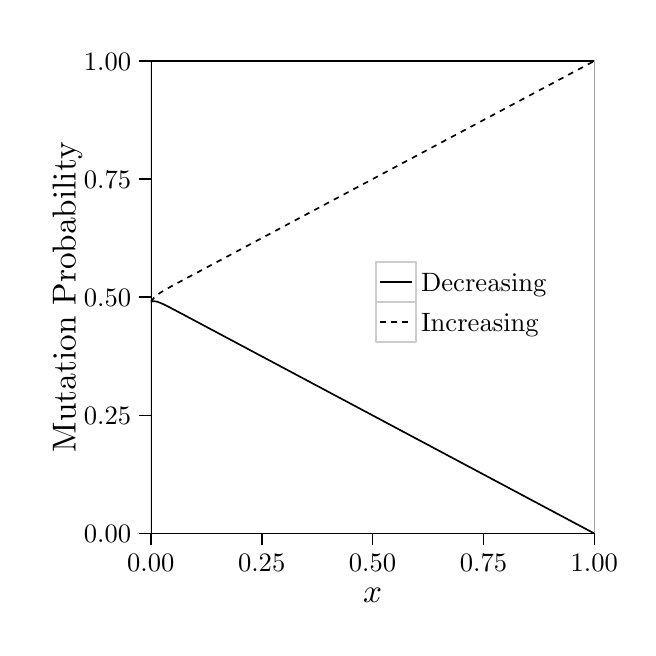
\begin{tikzpicture}[x=1pt,y=1pt]
\definecolor[named]{fillColor}{rgb}{1.00,1.00,1.00}
\path[use as bounding box,fill=fillColor,fill opacity=0.00] (0,0) rectangle (216.81,216.81);
\begin{scope}
\path[clip] (  0.00,  0.00) rectangle (216.81,216.81);
\definecolor[named]{drawColor}{rgb}{1.00,1.00,1.00}
\definecolor[named]{fillColor}{rgb}{1.00,1.00,1.00}

\path[draw=drawColor,line width= 0.6pt,line join=round,line cap=round,fill=fillColor] ( -0.00,  0.00) rectangle (216.81,216.81);
\end{scope}
\begin{scope}
\path[clip] ( 44.49, 34.03) rectangle (204.76,204.77);
\definecolor[named]{fillColor}{rgb}{1.00,1.00,1.00}

\path[fill=fillColor] ( 44.49, 34.03) rectangle (204.76,204.77);
\definecolor[named]{drawColor}{rgb}{0.00,0.00,0.00}

\path[draw=drawColor,line width= 0.6pt,line join=round] ( 44.49,117.69) --
	( 44.65,117.77) --
	( 44.81,117.83) --
	( 44.97,117.88) --
	( 45.13,117.91) --
	( 45.29,117.94) --
	( 45.45,117.95) --
	( 45.61,117.95) --
	( 45.77,117.95) --
	( 45.93,117.94) --
	( 46.09,117.92) --
	( 46.25,117.89) --
	( 46.41,117.86) --
	( 46.57,117.82) --
	( 46.73,117.78) --
	( 46.89,117.74) --
	( 47.05,117.69) --
	( 47.21,117.64) --
	( 47.37,117.58) --
	( 47.53,117.52) --
	( 47.69,117.46) --
	( 47.85,117.40) --
	( 48.01,117.33) --
	( 48.17,117.27) --
	( 48.33,117.20) --
	( 48.49,117.13) --
	( 48.65,117.05) --
	( 48.81,116.98) --
	( 48.97,116.91) --
	( 49.13,116.83) --
	( 49.29,116.75) --
	( 49.45,116.68) --
	( 49.61,116.60) --
	( 49.77,116.52) --
	( 49.93,116.44) --
	( 50.10,116.36) --
	( 50.26,116.28) --
	( 50.42,116.20) --
	( 50.58,116.12) --
	( 50.74,116.04) --
	( 50.90,115.95) --
	( 51.06,115.87) --
	( 51.22,115.79) --
	( 51.38,115.71) --
	( 51.54,115.62) --
	( 51.70,115.54) --
	( 51.86,115.46) --
	( 52.02,115.37) --
	( 52.18,115.29) --
	( 52.34,115.20) --
	( 52.50,115.12) --
	( 52.66,115.04) --
	( 52.82,114.95) --
	( 52.98,114.87) --
	( 53.14,114.78) --
	( 53.30,114.70) --
	( 53.46,114.61) --
	( 53.62,114.53) --
	( 53.78,114.44) --
	( 53.94,114.36) --
	( 54.10,114.27) --
	( 54.26,114.19) --
	( 54.42,114.10) --
	( 54.58,114.02) --
	( 54.74,113.93) --
	( 54.90,113.85) --
	( 55.06,113.76) --
	( 55.22,113.68) --
	( 55.38,113.59) --
	( 55.54,113.51) --
	( 55.70,113.42) --
	( 55.87,113.34) --
	( 56.03,113.25) --
	( 56.19,113.17) --
	( 56.35,113.08) --
	( 56.51,113.00) --
	( 56.67,112.91) --
	( 56.83,112.83) --
	( 56.99,112.74) --
	( 57.15,112.66) --
	( 57.31,112.57) --
	( 57.47,112.48) --
	( 57.63,112.40) --
	( 57.79,112.31) --
	( 57.95,112.23) --
	( 58.11,112.14) --
	( 58.27,112.06) --
	( 58.43,111.97) --
	( 58.59,111.89) --
	( 58.75,111.80) --
	( 58.91,111.72) --
	( 59.07,111.63) --
	( 59.23,111.55) --
	( 59.39,111.46) --
	( 59.55,111.38) --
	( 59.71,111.29) --
	( 59.87,111.20) --
	( 60.03,111.12) --
	( 60.19,111.03) --
	( 60.35,110.95) --
	( 60.51,110.86) --
	( 60.67,110.78) --
	( 60.83,110.69) --
	( 60.99,110.61) --
	( 61.15,110.52) --
	( 61.31,110.44) --
	( 61.48,110.35) --
	( 61.64,110.27) --
	( 61.80,110.18) --
	( 61.96,110.09) --
	( 62.12,110.01) --
	( 62.28,109.92) --
	( 62.44,109.84) --
	( 62.60,109.75) --
	( 62.76,109.67) --
	( 62.92,109.58) --
	( 63.08,109.50) --
	( 63.24,109.41) --
	( 63.40,109.33) --
	( 63.56,109.24) --
	( 63.72,109.16) --
	( 63.88,109.07) --
	( 64.04,108.99) --
	( 64.20,108.90) --
	( 64.36,108.81) --
	( 64.52,108.73) --
	( 64.68,108.64) --
	( 64.84,108.56) --
	( 65.00,108.47) --
	( 65.16,108.39) --
	( 65.32,108.30) --
	( 65.48,108.22) --
	( 65.64,108.13) --
	( 65.80,108.05) --
	( 65.96,107.96) --
	( 66.12,107.88) --
	( 66.28,107.79) --
	( 66.44,107.70) --
	( 66.60,107.62) --
	( 66.76,107.53) --
	( 66.92,107.45) --
	( 67.08,107.36) --
	( 67.25,107.28) --
	( 67.41,107.19) --
	( 67.57,107.11) --
	( 67.73,107.02) --
	( 67.89,106.94) --
	( 68.05,106.85) --
	( 68.21,106.77) --
	( 68.37,106.68) --
	( 68.53,106.60) --
	( 68.69,106.51) --
	( 68.85,106.42) --
	( 69.01,106.34) --
	( 69.17,106.25) --
	( 69.33,106.17) --
	( 69.49,106.08) --
	( 69.65,106.00) --
	( 69.81,105.91) --
	( 69.97,105.83) --
	( 70.13,105.74) --
	( 70.29,105.66) --
	( 70.45,105.57) --
	( 70.61,105.49) --
	( 70.77,105.40) --
	( 70.93,105.31) --
	( 71.09,105.23) --
	( 71.25,105.14) --
	( 71.41,105.06) --
	( 71.57,104.97) --
	( 71.73,104.89) --
	( 71.89,104.80) --
	( 72.05,104.72) --
	( 72.21,104.63) --
	( 72.37,104.55) --
	( 72.53,104.46) --
	( 72.69,104.38) --
	( 72.85,104.29) --
	( 73.02,104.20) --
	( 73.18,104.12) --
	( 73.34,104.03) --
	( 73.50,103.95) --
	( 73.66,103.86) --
	( 73.82,103.78) --
	( 73.98,103.69) --
	( 74.14,103.61) --
	( 74.30,103.52) --
	( 74.46,103.44) --
	( 74.62,103.35) --
	( 74.78,103.27) --
	( 74.94,103.18) --
	( 75.10,103.10) --
	( 75.26,103.01) --
	( 75.42,102.92) --
	( 75.58,102.84) --
	( 75.74,102.75) --
	( 75.90,102.67) --
	( 76.06,102.58) --
	( 76.22,102.50) --
	( 76.38,102.41) --
	( 76.54,102.33) --
	( 76.70,102.24) --
	( 76.86,102.16) --
	( 77.02,102.07) --
	( 77.18,101.99) --
	( 77.34,101.90) --
	( 77.50,101.81) --
	( 77.66,101.73) --
	( 77.82,101.64) --
	( 77.98,101.56) --
	( 78.14,101.47) --
	( 78.30,101.39) --
	( 78.46,101.30) --
	( 78.62,101.22) --
	( 78.79,101.13) --
	( 78.95,101.05) --
	( 79.11,100.96) --
	( 79.27,100.88) --
	( 79.43,100.79) --
	( 79.59,100.70) --
	( 79.75,100.62) --
	( 79.91,100.53) --
	( 80.07,100.45) --
	( 80.23,100.36) --
	( 80.39,100.28) --
	( 80.55,100.19) --
	( 80.71,100.11) --
	( 80.87,100.02) --
	( 81.03, 99.94) --
	( 81.19, 99.85) --
	( 81.35, 99.77) --
	( 81.51, 99.68) --
	( 81.67, 99.60) --
	( 81.83, 99.51) --
	( 81.99, 99.42) --
	( 82.15, 99.34) --
	( 82.31, 99.25) --
	( 82.47, 99.17) --
	( 82.63, 99.08) --
	( 82.79, 99.00) --
	( 82.95, 98.91) --
	( 83.11, 98.83) --
	( 83.27, 98.74) --
	( 83.43, 98.66) --
	( 83.59, 98.57) --
	( 83.75, 98.49) --
	( 83.91, 98.40) --
	( 84.07, 98.31) --
	( 84.23, 98.23) --
	( 84.40, 98.14) --
	( 84.56, 98.06) --
	( 84.72, 97.97) --
	( 84.88, 97.89) --
	( 85.04, 97.80) --
	( 85.20, 97.72) --
	( 85.36, 97.63) --
	( 85.52, 97.55) --
	( 85.68, 97.46) --
	( 85.84, 97.38) --
	( 86.00, 97.29) --
	( 86.16, 97.20) --
	( 86.32, 97.12) --
	( 86.48, 97.03) --
	( 86.64, 96.95) --
	( 86.80, 96.86) --
	( 86.96, 96.78) --
	( 87.12, 96.69) --
	( 87.28, 96.61) --
	( 87.44, 96.52) --
	( 87.60, 96.44) --
	( 87.76, 96.35) --
	( 87.92, 96.27) --
	( 88.08, 96.18) --
	( 88.24, 96.10) --
	( 88.40, 96.01) --
	( 88.56, 95.92) --
	( 88.72, 95.84) --
	( 88.88, 95.75) --
	( 89.04, 95.67) --
	( 89.20, 95.58) --
	( 89.36, 95.50) --
	( 89.52, 95.41) --
	( 89.68, 95.33) --
	( 89.84, 95.24) --
	( 90.00, 95.16) --
	( 90.17, 95.07) --
	( 90.33, 94.99) --
	( 90.49, 94.90) --
	( 90.65, 94.81) --
	( 90.81, 94.73) --
	( 90.97, 94.64) --
	( 91.13, 94.56) --
	( 91.29, 94.47) --
	( 91.45, 94.39) --
	( 91.61, 94.30) --
	( 91.77, 94.22) --
	( 91.93, 94.13) --
	( 92.09, 94.05) --
	( 92.25, 93.96) --
	( 92.41, 93.88) --
	( 92.57, 93.79) --
	( 92.73, 93.70) --
	( 92.89, 93.62) --
	( 93.05, 93.53) --
	( 93.21, 93.45) --
	( 93.37, 93.36) --
	( 93.53, 93.28) --
	( 93.69, 93.19) --
	( 93.85, 93.11) --
	( 94.01, 93.02) --
	( 94.17, 92.94) --
	( 94.33, 92.85) --
	( 94.49, 92.77) --
	( 94.65, 92.68) --
	( 94.81, 92.60) --
	( 94.97, 92.51) --
	( 95.13, 92.42) --
	( 95.29, 92.34) --
	( 95.45, 92.25) --
	( 95.61, 92.17) --
	( 95.77, 92.08) --
	( 95.94, 92.00) --
	( 96.10, 91.91) --
	( 96.26, 91.83) --
	( 96.42, 91.74) --
	( 96.58, 91.66) --
	( 96.74, 91.57) --
	( 96.90, 91.49) --
	( 97.06, 91.40) --
	( 97.22, 91.31) --
	( 97.38, 91.23) --
	( 97.54, 91.14) --
	( 97.70, 91.06) --
	( 97.86, 90.97) --
	( 98.02, 90.89) --
	( 98.18, 90.80) --
	( 98.34, 90.72) --
	( 98.50, 90.63) --
	( 98.66, 90.55) --
	( 98.82, 90.46) --
	( 98.98, 90.38) --
	( 99.14, 90.29) --
	( 99.30, 90.20) --
	( 99.46, 90.12) --
	( 99.62, 90.03) --
	( 99.78, 89.95) --
	( 99.94, 89.86) --
	(100.10, 89.78) --
	(100.26, 89.69) --
	(100.42, 89.61) --
	(100.58, 89.52) --
	(100.74, 89.44) --
	(100.90, 89.35) --
	(101.06, 89.27) --
	(101.22, 89.18) --
	(101.38, 89.10) --
	(101.54, 89.01) --
	(101.71, 88.92) --
	(101.87, 88.84) --
	(102.03, 88.75) --
	(102.19, 88.67) --
	(102.35, 88.58) --
	(102.51, 88.50) --
	(102.67, 88.41) --
	(102.83, 88.33) --
	(102.99, 88.24) --
	(103.15, 88.16) --
	(103.31, 88.07) --
	(103.47, 87.99) --
	(103.63, 87.90) --
	(103.79, 87.81) --
	(103.95, 87.73) --
	(104.11, 87.64) --
	(104.27, 87.56) --
	(104.43, 87.47) --
	(104.59, 87.39) --
	(104.75, 87.30) --
	(104.91, 87.22) --
	(105.07, 87.13) --
	(105.23, 87.05) --
	(105.39, 86.96) --
	(105.55, 86.88) --
	(105.71, 86.79) --
	(105.87, 86.70) --
	(106.03, 86.62) --
	(106.19, 86.53) --
	(106.35, 86.45) --
	(106.51, 86.36) --
	(106.67, 86.28) --
	(106.83, 86.19) --
	(106.99, 86.11) --
	(107.15, 86.02) --
	(107.32, 85.94) --
	(107.48, 85.85) --
	(107.64, 85.77) --
	(107.80, 85.68) --
	(107.96, 85.60) --
	(108.12, 85.51) --
	(108.28, 85.42) --
	(108.44, 85.34) --
	(108.60, 85.25) --
	(108.76, 85.17) --
	(108.92, 85.08) --
	(109.08, 85.00) --
	(109.24, 84.91) --
	(109.40, 84.83) --
	(109.56, 84.74) --
	(109.72, 84.66) --
	(109.88, 84.57) --
	(110.04, 84.49) --
	(110.20, 84.40) --
	(110.36, 84.31) --
	(110.52, 84.23) --
	(110.68, 84.14) --
	(110.84, 84.06) --
	(111.00, 83.97) --
	(111.16, 83.89) --
	(111.32, 83.80) --
	(111.48, 83.72) --
	(111.64, 83.63) --
	(111.80, 83.55) --
	(111.96, 83.46) --
	(112.12, 83.38) --
	(112.28, 83.29) --
	(112.44, 83.20) --
	(112.60, 83.12) --
	(112.76, 83.03) --
	(112.92, 82.95) --
	(113.09, 82.86) --
	(113.25, 82.78) --
	(113.41, 82.69) --
	(113.57, 82.61) --
	(113.73, 82.52) --
	(113.89, 82.44) --
	(114.05, 82.35) --
	(114.21, 82.27) --
	(114.37, 82.18) --
	(114.53, 82.10) --
	(114.69, 82.01) --
	(114.85, 81.92) --
	(115.01, 81.84) --
	(115.17, 81.75) --
	(115.33, 81.67) --
	(115.49, 81.58) --
	(115.65, 81.50) --
	(115.81, 81.41) --
	(115.97, 81.33) --
	(116.13, 81.24) --
	(116.29, 81.16) --
	(116.45, 81.07) --
	(116.61, 80.99) --
	(116.77, 80.90) --
	(116.93, 80.81) --
	(117.09, 80.73) --
	(117.25, 80.64) --
	(117.41, 80.56) --
	(117.57, 80.47) --
	(117.73, 80.39) --
	(117.89, 80.30) --
	(118.05, 80.22) --
	(118.21, 80.13) --
	(118.37, 80.05) --
	(118.53, 79.96) --
	(118.69, 79.88) --
	(118.86, 79.79) --
	(119.02, 79.70) --
	(119.18, 79.62) --
	(119.34, 79.53) --
	(119.50, 79.45) --
	(119.66, 79.36) --
	(119.82, 79.28) --
	(119.98, 79.19) --
	(120.14, 79.11) --
	(120.30, 79.02) --
	(120.46, 78.94) --
	(120.62, 78.85) --
	(120.78, 78.77) --
	(120.94, 78.68) --
	(121.10, 78.60) --
	(121.26, 78.51) --
	(121.42, 78.42) --
	(121.58, 78.34) --
	(121.74, 78.25) --
	(121.90, 78.17) --
	(122.06, 78.08) --
	(122.22, 78.00) --
	(122.38, 77.91) --
	(122.54, 77.83) --
	(122.70, 77.74) --
	(122.86, 77.66) --
	(123.02, 77.57) --
	(123.18, 77.49) --
	(123.34, 77.40) --
	(123.50, 77.31) --
	(123.66, 77.23) --
	(123.82, 77.14) --
	(123.98, 77.06) --
	(124.14, 76.97) --
	(124.30, 76.89) --
	(124.46, 76.80) --
	(124.63, 76.72) --
	(124.79, 76.63) --
	(124.95, 76.55) --
	(125.11, 76.46) --
	(125.27, 76.38) --
	(125.43, 76.29) --
	(125.59, 76.20) --
	(125.75, 76.12) --
	(125.91, 76.03) --
	(126.07, 75.95) --
	(126.23, 75.86) --
	(126.39, 75.78) --
	(126.55, 75.69) --
	(126.71, 75.61) --
	(126.87, 75.52) --
	(127.03, 75.44) --
	(127.19, 75.35) --
	(127.35, 75.27) --
	(127.51, 75.18) --
	(127.67, 75.10) --
	(127.83, 75.01) --
	(127.99, 74.92) --
	(128.15, 74.84) --
	(128.31, 74.75) --
	(128.47, 74.67) --
	(128.63, 74.58) --
	(128.79, 74.50) --
	(128.95, 74.41) --
	(129.11, 74.33) --
	(129.27, 74.24) --
	(129.43, 74.16) --
	(129.59, 74.07) --
	(129.75, 73.99) --
	(129.91, 73.90) --
	(130.07, 73.81) --
	(130.23, 73.73) --
	(130.40, 73.64) --
	(130.56, 73.56) --
	(130.72, 73.47) --
	(130.88, 73.39) --
	(131.04, 73.30) --
	(131.20, 73.22) --
	(131.36, 73.13) --
	(131.52, 73.05) --
	(131.68, 72.96) --
	(131.84, 72.88) --
	(132.00, 72.79) --
	(132.16, 72.71) --
	(132.32, 72.62) --
	(132.48, 72.53) --
	(132.64, 72.45) --
	(132.80, 72.36) --
	(132.96, 72.28) --
	(133.12, 72.19) --
	(133.28, 72.11) --
	(133.44, 72.02) --
	(133.60, 71.94) --
	(133.76, 71.85) --
	(133.92, 71.77) --
	(134.08, 71.68) --
	(134.24, 71.60) --
	(134.40, 71.51) --
	(134.56, 71.42) --
	(134.72, 71.34) --
	(134.88, 71.25) --
	(135.04, 71.17) --
	(135.20, 71.08) --
	(135.36, 71.00) --
	(135.52, 70.91) --
	(135.68, 70.83) --
	(135.84, 70.74) --
	(136.01, 70.66) --
	(136.17, 70.57) --
	(136.33, 70.49) --
	(136.49, 70.40) --
	(136.65, 70.31) --
	(136.81, 70.23) --
	(136.97, 70.14) --
	(137.13, 70.06) --
	(137.29, 69.97) --
	(137.45, 69.89) --
	(137.61, 69.80) --
	(137.77, 69.72) --
	(137.93, 69.63) --
	(138.09, 69.55) --
	(138.25, 69.46) --
	(138.41, 69.38) --
	(138.57, 69.29) --
	(138.73, 69.21) --
	(138.89, 69.12) --
	(139.05, 69.03) --
	(139.21, 68.95) --
	(139.37, 68.86) --
	(139.53, 68.78) --
	(139.69, 68.69) --
	(139.85, 68.61) --
	(140.01, 68.52) --
	(140.17, 68.44) --
	(140.33, 68.35) --
	(140.49, 68.27) --
	(140.65, 68.18) --
	(140.81, 68.10) --
	(140.97, 68.01) --
	(141.13, 67.92) --
	(141.29, 67.84) --
	(141.45, 67.75) --
	(141.61, 67.67) --
	(141.78, 67.58) --
	(141.94, 67.50) --
	(142.10, 67.41) --
	(142.26, 67.33) --
	(142.42, 67.24) --
	(142.58, 67.16) --
	(142.74, 67.07) --
	(142.90, 66.99) --
	(143.06, 66.90) --
	(143.22, 66.81) --
	(143.38, 66.73) --
	(143.54, 66.64) --
	(143.70, 66.56) --
	(143.86, 66.47) --
	(144.02, 66.39) --
	(144.18, 66.30) --
	(144.34, 66.22) --
	(144.50, 66.13) --
	(144.66, 66.05) --
	(144.82, 65.96) --
	(144.98, 65.88) --
	(145.14, 65.79) --
	(145.30, 65.71) --
	(145.46, 65.62) --
	(145.62, 65.53) --
	(145.78, 65.45) --
	(145.94, 65.36) --
	(146.10, 65.28) --
	(146.26, 65.19) --
	(146.42, 65.11) --
	(146.58, 65.02) --
	(146.74, 64.94) --
	(146.90, 64.85) --
	(147.06, 64.77) --
	(147.22, 64.68) --
	(147.38, 64.60) --
	(147.55, 64.51) --
	(147.71, 64.42) --
	(147.87, 64.34) --
	(148.03, 64.25) --
	(148.19, 64.17) --
	(148.35, 64.08) --
	(148.51, 64.00) --
	(148.67, 63.91) --
	(148.83, 63.83) --
	(148.99, 63.74) --
	(149.15, 63.66) --
	(149.31, 63.57) --
	(149.47, 63.49) --
	(149.63, 63.40) --
	(149.79, 63.31) --
	(149.95, 63.23) --
	(150.11, 63.14) --
	(150.27, 63.06) --
	(150.43, 62.97) --
	(150.59, 62.89) --
	(150.75, 62.80) --
	(150.91, 62.72) --
	(151.07, 62.63) --
	(151.23, 62.55) --
	(151.39, 62.46) --
	(151.55, 62.38) --
	(151.71, 62.29) --
	(151.87, 62.21) --
	(152.03, 62.12) --
	(152.19, 62.03) --
	(152.35, 61.95) --
	(152.51, 61.86) --
	(152.67, 61.78) --
	(152.83, 61.69) --
	(152.99, 61.61) --
	(153.15, 61.52) --
	(153.32, 61.44) --
	(153.48, 61.35) --
	(153.64, 61.27) --
	(153.80, 61.18) --
	(153.96, 61.10) --
	(154.12, 61.01) --
	(154.28, 60.92) --
	(154.44, 60.84) --
	(154.60, 60.75) --
	(154.76, 60.67) --
	(154.92, 60.58) --
	(155.08, 60.50) --
	(155.24, 60.41) --
	(155.40, 60.33) --
	(155.56, 60.24) --
	(155.72, 60.16) --
	(155.88, 60.07) --
	(156.04, 59.99) --
	(156.20, 59.90) --
	(156.36, 59.81) --
	(156.52, 59.73) --
	(156.68, 59.64) --
	(156.84, 59.56) --
	(157.00, 59.47) --
	(157.16, 59.39) --
	(157.32, 59.30) --
	(157.48, 59.22) --
	(157.64, 59.13) --
	(157.80, 59.05) --
	(157.96, 58.96) --
	(158.12, 58.88) --
	(158.28, 58.79) --
	(158.44, 58.71) --
	(158.60, 58.62) --
	(158.76, 58.53) --
	(158.93, 58.45) --
	(159.09, 58.36) --
	(159.25, 58.28) --
	(159.41, 58.19) --
	(159.57, 58.11) --
	(159.73, 58.02) --
	(159.89, 57.94) --
	(160.05, 57.85) --
	(160.21, 57.77) --
	(160.37, 57.68) --
	(160.53, 57.60) --
	(160.69, 57.51) --
	(160.85, 57.42) --
	(161.01, 57.34) --
	(161.17, 57.25) --
	(161.33, 57.17) --
	(161.49, 57.08) --
	(161.65, 57.00) --
	(161.81, 56.91) --
	(161.97, 56.83) --
	(162.13, 56.74) --
	(162.29, 56.66) --
	(162.45, 56.57) --
	(162.61, 56.49) --
	(162.77, 56.40) --
	(162.93, 56.31) --
	(163.09, 56.23) --
	(163.25, 56.14) --
	(163.41, 56.06) --
	(163.57, 55.97) --
	(163.73, 55.89) --
	(163.89, 55.80) --
	(164.05, 55.72) --
	(164.21, 55.63) --
	(164.37, 55.55) --
	(164.53, 55.46) --
	(164.70, 55.38) --
	(164.86, 55.29) --
	(165.02, 55.21) --
	(165.18, 55.12) --
	(165.34, 55.03) --
	(165.50, 54.95) --
	(165.66, 54.86) --
	(165.82, 54.78) --
	(165.98, 54.69) --
	(166.14, 54.61) --
	(166.30, 54.52) --
	(166.46, 54.44) --
	(166.62, 54.35) --
	(166.78, 54.27) --
	(166.94, 54.18) --
	(167.10, 54.10) --
	(167.26, 54.01) --
	(167.42, 53.92) --
	(167.58, 53.84) --
	(167.74, 53.75) --
	(167.90, 53.67) --
	(168.06, 53.58) --
	(168.22, 53.50) --
	(168.38, 53.41) --
	(168.54, 53.33) --
	(168.70, 53.24) --
	(168.86, 53.16) --
	(169.02, 53.07) --
	(169.18, 52.99) --
	(169.34, 52.90) --
	(169.50, 52.81) --
	(169.66, 52.73) --
	(169.82, 52.64) --
	(169.98, 52.56) --
	(170.14, 52.47) --
	(170.30, 52.39) --
	(170.47, 52.30) --
	(170.63, 52.22) --
	(170.79, 52.13) --
	(170.95, 52.05) --
	(171.11, 51.96) --
	(171.27, 51.88) --
	(171.43, 51.79) --
	(171.59, 51.71) --
	(171.75, 51.62) --
	(171.91, 51.53) --
	(172.07, 51.45) --
	(172.23, 51.36) --
	(172.39, 51.28) --
	(172.55, 51.19) --
	(172.71, 51.11) --
	(172.87, 51.02) --
	(173.03, 50.94) --
	(173.19, 50.85) --
	(173.35, 50.77) --
	(173.51, 50.68) --
	(173.67, 50.60) --
	(173.83, 50.51) --
	(173.99, 50.42) --
	(174.15, 50.34) --
	(174.31, 50.25) --
	(174.47, 50.17) --
	(174.63, 50.08) --
	(174.79, 50.00) --
	(174.95, 49.91) --
	(175.11, 49.83) --
	(175.27, 49.74) --
	(175.43, 49.66) --
	(175.59, 49.57) --
	(175.75, 49.49) --
	(175.91, 49.40) --
	(176.07, 49.31) --
	(176.24, 49.23) --
	(176.40, 49.14) --
	(176.56, 49.06) --
	(176.72, 48.97) --
	(176.88, 48.89) --
	(177.04, 48.80) --
	(177.20, 48.72) --
	(177.36, 48.63) --
	(177.52, 48.55) --
	(177.68, 48.46) --
	(177.84, 48.38) --
	(178.00, 48.29) --
	(178.16, 48.21) --
	(178.32, 48.12) --
	(178.48, 48.03) --
	(178.64, 47.95) --
	(178.80, 47.86) --
	(178.96, 47.78) --
	(179.12, 47.69) --
	(179.28, 47.61) --
	(179.44, 47.52) --
	(179.60, 47.44) --
	(179.76, 47.35) --
	(179.92, 47.27) --
	(180.08, 47.18) --
	(180.24, 47.10) --
	(180.40, 47.01) --
	(180.56, 46.92) --
	(180.72, 46.84) --
	(180.88, 46.75) --
	(181.04, 46.67) --
	(181.20, 46.58) --
	(181.36, 46.50) --
	(181.52, 46.41) --
	(181.68, 46.33) --
	(181.85, 46.24) --
	(182.01, 46.16) --
	(182.17, 46.07) --
	(182.33, 45.99) --
	(182.49, 45.90) --
	(182.65, 45.81) --
	(182.81, 45.73) --
	(182.97, 45.64) --
	(183.13, 45.56) --
	(183.29, 45.47) --
	(183.45, 45.39) --
	(183.61, 45.30) --
	(183.77, 45.22) --
	(183.93, 45.13) --
	(184.09, 45.05) --
	(184.25, 44.96) --
	(184.41, 44.88) --
	(184.57, 44.79) --
	(184.73, 44.71) --
	(184.89, 44.62) --
	(185.05, 44.53) --
	(185.21, 44.45) --
	(185.37, 44.36) --
	(185.53, 44.28) --
	(185.69, 44.19) --
	(185.85, 44.11) --
	(186.01, 44.02) --
	(186.17, 43.94) --
	(186.33, 43.85) --
	(186.49, 43.77) --
	(186.65, 43.68) --
	(186.81, 43.60) --
	(186.97, 43.51) --
	(187.13, 43.42) --
	(187.29, 43.34) --
	(187.45, 43.25) --
	(187.62, 43.17) --
	(187.78, 43.08) --
	(187.94, 43.00) --
	(188.10, 42.91) --
	(188.26, 42.83) --
	(188.42, 42.74) --
	(188.58, 42.66) --
	(188.74, 42.57) --
	(188.90, 42.49) --
	(189.06, 42.40) --
	(189.22, 42.31) --
	(189.38, 42.23) --
	(189.54, 42.14) --
	(189.70, 42.06) --
	(189.86, 41.97) --
	(190.02, 41.89) --
	(190.18, 41.80) --
	(190.34, 41.72) --
	(190.50, 41.63) --
	(190.66, 41.55) --
	(190.82, 41.46) --
	(190.98, 41.38) --
	(191.14, 41.29) --
	(191.30, 41.21) --
	(191.46, 41.12) --
	(191.62, 41.03) --
	(191.78, 40.95) --
	(191.94, 40.86) --
	(192.10, 40.78) --
	(192.26, 40.69) --
	(192.42, 40.61) --
	(192.58, 40.52) --
	(192.74, 40.44) --
	(192.90, 40.35) --
	(193.06, 40.27) --
	(193.22, 40.18) --
	(193.39, 40.10) --
	(193.55, 40.01) --
	(193.71, 39.92) --
	(193.87, 39.84) --
	(194.03, 39.75) --
	(194.19, 39.67) --
	(194.35, 39.58) --
	(194.51, 39.50) --
	(194.67, 39.41) --
	(194.83, 39.33) --
	(194.99, 39.24) --
	(195.15, 39.16) --
	(195.31, 39.07) --
	(195.47, 38.99) --
	(195.63, 38.90) --
	(195.79, 38.82) --
	(195.95, 38.73) --
	(196.11, 38.64) --
	(196.27, 38.56) --
	(196.43, 38.47) --
	(196.59, 38.39) --
	(196.75, 38.30) --
	(196.91, 38.22) --
	(197.07, 38.13) --
	(197.23, 38.05) --
	(197.39, 37.96) --
	(197.55, 37.88) --
	(197.71, 37.79) --
	(197.87, 37.71) --
	(198.03, 37.62) --
	(198.19, 37.53) --
	(198.35, 37.45) --
	(198.51, 37.36) --
	(198.67, 37.28) --
	(198.83, 37.19) --
	(198.99, 37.11) --
	(199.16, 37.02) --
	(199.32, 36.94) --
	(199.48, 36.85) --
	(199.64, 36.77) --
	(199.80, 36.68) --
	(199.96, 36.60) --
	(200.12, 36.51) --
	(200.28, 36.42) --
	(200.44, 36.34) --
	(200.60, 36.25) --
	(200.76, 36.17) --
	(200.92, 36.08) --
	(201.08, 36.00) --
	(201.24, 35.91) --
	(201.40, 35.83) --
	(201.56, 35.74) --
	(201.72, 35.66) --
	(201.88, 35.57) --
	(202.04, 35.49) --
	(202.20, 35.40) --
	(202.36, 35.32) --
	(202.52, 35.23) --
	(202.68, 35.14) --
	(202.84, 35.06) --
	(203.00, 34.97) --
	(203.16, 34.89) --
	(203.32, 34.80) --
	(203.48, 34.72) --
	(203.64, 34.63) --
	(203.80, 34.55) --
	(203.96, 34.46) --
	(204.12, 34.38) --
	(204.28, 34.29) --
	(204.44, 34.21) --
	(204.60, 34.12) --
	(204.76, 34.03);

\path[draw=drawColor,line width= 0.6pt,dash pattern=on 2pt off 2pt ,line join=round] ( 44.49,117.69) --
	( 44.65,117.94) --
	( 44.81,118.17) --
	( 44.97,118.39) --
	( 45.13,118.60) --
	( 45.29,118.79) --
	( 45.45,118.97) --
	( 45.61,119.15) --
	( 45.77,119.32) --
	( 45.93,119.47) --
	( 46.09,119.63) --
	( 46.25,119.77) --
	( 46.41,119.91) --
	( 46.57,120.04) --
	( 46.73,120.17) --
	( 46.89,120.30) --
	( 47.05,120.42) --
	( 47.21,120.54) --
	( 47.37,120.65) --
	( 47.53,120.77) --
	( 47.69,120.88) --
	( 47.85,120.98) --
	( 48.01,121.09) --
	( 48.17,121.19) --
	( 48.33,121.29) --
	( 48.49,121.39) --
	( 48.65,121.49) --
	( 48.81,121.59) --
	( 48.97,121.69) --
	( 49.13,121.78) --
	( 49.29,121.88) --
	( 49.45,121.97) --
	( 49.61,122.06) --
	( 49.77,122.15) --
	( 49.93,122.25) --
	( 50.10,122.34) --
	( 50.26,122.43) --
	( 50.42,122.52) --
	( 50.58,122.61) --
	( 50.74,122.69) --
	( 50.90,122.78) --
	( 51.06,122.87) --
	( 51.22,122.96) --
	( 51.38,123.05) --
	( 51.54,123.13) --
	( 51.70,123.22) --
	( 51.86,123.31) --
	( 52.02,123.40) --
	( 52.18,123.48) --
	( 52.34,123.57) --
	( 52.50,123.66) --
	( 52.66,123.74) --
	( 52.82,123.83) --
	( 52.98,123.92) --
	( 53.14,124.00) --
	( 53.30,124.09) --
	( 53.46,124.17) --
	( 53.62,124.26) --
	( 53.78,124.35) --
	( 53.94,124.43) --
	( 54.10,124.52) --
	( 54.26,124.60) --
	( 54.42,124.69) --
	( 54.58,124.77) --
	( 54.74,124.86) --
	( 54.90,124.95) --
	( 55.06,125.03) --
	( 55.22,125.12) --
	( 55.38,125.20) --
	( 55.54,125.29) --
	( 55.70,125.37) --
	( 55.87,125.46) --
	( 56.03,125.54) --
	( 56.19,125.63) --
	( 56.35,125.72) --
	( 56.51,125.80) --
	( 56.67,125.89) --
	( 56.83,125.97) --
	( 56.99,126.06) --
	( 57.15,126.14) --
	( 57.31,126.23) --
	( 57.47,126.31) --
	( 57.63,126.40) --
	( 57.79,126.48) --
	( 57.95,126.57) --
	( 58.11,126.66) --
	( 58.27,126.74) --
	( 58.43,126.83) --
	( 58.59,126.91) --
	( 58.75,127.00) --
	( 58.91,127.08) --
	( 59.07,127.17) --
	( 59.23,127.25) --
	( 59.39,127.34) --
	( 59.55,127.42) --
	( 59.71,127.51) --
	( 59.87,127.59) --
	( 60.03,127.68) --
	( 60.19,127.77) --
	( 60.35,127.85) --
	( 60.51,127.94) --
	( 60.67,128.02) --
	( 60.83,128.11) --
	( 60.99,128.19) --
	( 61.15,128.28) --
	( 61.31,128.36) --
	( 61.48,128.45) --
	( 61.64,128.53) --
	( 61.80,128.62) --
	( 61.96,128.70) --
	( 62.12,128.79) --
	( 62.28,128.88) --
	( 62.44,128.96) --
	( 62.60,129.05) --
	( 62.76,129.13) --
	( 62.92,129.22) --
	( 63.08,129.30) --
	( 63.24,129.39) --
	( 63.40,129.47) --
	( 63.56,129.56) --
	( 63.72,129.64) --
	( 63.88,129.73) --
	( 64.04,129.81) --
	( 64.20,129.90) --
	( 64.36,129.99) --
	( 64.52,130.07) --
	( 64.68,130.16) --
	( 64.84,130.24) --
	( 65.00,130.33) --
	( 65.16,130.41) --
	( 65.32,130.50) --
	( 65.48,130.58) --
	( 65.64,130.67) --
	( 65.80,130.75) --
	( 65.96,130.84) --
	( 66.12,130.92) --
	( 66.28,131.01) --
	( 66.44,131.09) --
	( 66.60,131.18) --
	( 66.76,131.27) --
	( 66.92,131.35) --
	( 67.08,131.44) --
	( 67.25,131.52) --
	( 67.41,131.61) --
	( 67.57,131.69) --
	( 67.73,131.78) --
	( 67.89,131.86) --
	( 68.05,131.95) --
	( 68.21,132.03) --
	( 68.37,132.12) --
	( 68.53,132.20) --
	( 68.69,132.29) --
	( 68.85,132.38) --
	( 69.01,132.46) --
	( 69.17,132.55) --
	( 69.33,132.63) --
	( 69.49,132.72) --
	( 69.65,132.80) --
	( 69.81,132.89) --
	( 69.97,132.97) --
	( 70.13,133.06) --
	( 70.29,133.14) --
	( 70.45,133.23) --
	( 70.61,133.31) --
	( 70.77,133.40) --
	( 70.93,133.49) --
	( 71.09,133.57) --
	( 71.25,133.66) --
	( 71.41,133.74) --
	( 71.57,133.83) --
	( 71.73,133.91) --
	( 71.89,134.00) --
	( 72.05,134.08) --
	( 72.21,134.17) --
	( 72.37,134.25) --
	( 72.53,134.34) --
	( 72.69,134.42) --
	( 72.85,134.51) --
	( 73.02,134.59) --
	( 73.18,134.68) --
	( 73.34,134.77) --
	( 73.50,134.85) --
	( 73.66,134.94) --
	( 73.82,135.02) --
	( 73.98,135.11) --
	( 74.14,135.19) --
	( 74.30,135.28) --
	( 74.46,135.36) --
	( 74.62,135.45) --
	( 74.78,135.53) --
	( 74.94,135.62) --
	( 75.10,135.70) --
	( 75.26,135.79) --
	( 75.42,135.88) --
	( 75.58,135.96) --
	( 75.74,136.05) --
	( 75.90,136.13) --
	( 76.06,136.22) --
	( 76.22,136.30) --
	( 76.38,136.39) --
	( 76.54,136.47) --
	( 76.70,136.56) --
	( 76.86,136.64) --
	( 77.02,136.73) --
	( 77.18,136.81) --
	( 77.34,136.90) --
	( 77.50,136.99) --
	( 77.66,137.07) --
	( 77.82,137.16) --
	( 77.98,137.24) --
	( 78.14,137.33) --
	( 78.30,137.41) --
	( 78.46,137.50) --
	( 78.62,137.58) --
	( 78.79,137.67) --
	( 78.95,137.75) --
	( 79.11,137.84) --
	( 79.27,137.92) --
	( 79.43,138.01) --
	( 79.59,138.09) --
	( 79.75,138.18) --
	( 79.91,138.27) --
	( 80.07,138.35) --
	( 80.23,138.44) --
	( 80.39,138.52) --
	( 80.55,138.61) --
	( 80.71,138.69) --
	( 80.87,138.78) --
	( 81.03,138.86) --
	( 81.19,138.95) --
	( 81.35,139.03) --
	( 81.51,139.12) --
	( 81.67,139.20) --
	( 81.83,139.29) --
	( 81.99,139.38) --
	( 82.15,139.46) --
	( 82.31,139.55) --
	( 82.47,139.63) --
	( 82.63,139.72) --
	( 82.79,139.80) --
	( 82.95,139.89) --
	( 83.11,139.97) --
	( 83.27,140.06) --
	( 83.43,140.14) --
	( 83.59,140.23) --
	( 83.75,140.31) --
	( 83.91,140.40) --
	( 84.07,140.48) --
	( 84.23,140.57) --
	( 84.40,140.66) --
	( 84.56,140.74) --
	( 84.72,140.83) --
	( 84.88,140.91) --
	( 85.04,141.00) --
	( 85.20,141.08) --
	( 85.36,141.17) --
	( 85.52,141.25) --
	( 85.68,141.34) --
	( 85.84,141.42) --
	( 86.00,141.51) --
	( 86.16,141.59) --
	( 86.32,141.68) --
	( 86.48,141.77) --
	( 86.64,141.85) --
	( 86.80,141.94) --
	( 86.96,142.02) --
	( 87.12,142.11) --
	( 87.28,142.19) --
	( 87.44,142.28) --
	( 87.60,142.36) --
	( 87.76,142.45) --
	( 87.92,142.53) --
	( 88.08,142.62) --
	( 88.24,142.70) --
	( 88.40,142.79) --
	( 88.56,142.88) --
	( 88.72,142.96) --
	( 88.88,143.05) --
	( 89.04,143.13) --
	( 89.20,143.22) --
	( 89.36,143.30) --
	( 89.52,143.39) --
	( 89.68,143.47) --
	( 89.84,143.56) --
	( 90.00,143.64) --
	( 90.17,143.73) --
	( 90.33,143.81) --
	( 90.49,143.90) --
	( 90.65,143.98) --
	( 90.81,144.07) --
	( 90.97,144.16) --
	( 91.13,144.24) --
	( 91.29,144.33) --
	( 91.45,144.41) --
	( 91.61,144.50) --
	( 91.77,144.58) --
	( 91.93,144.67) --
	( 92.09,144.75) --
	( 92.25,144.84) --
	( 92.41,144.92) --
	( 92.57,145.01) --
	( 92.73,145.09) --
	( 92.89,145.18) --
	( 93.05,145.27) --
	( 93.21,145.35) --
	( 93.37,145.44) --
	( 93.53,145.52) --
	( 93.69,145.61) --
	( 93.85,145.69) --
	( 94.01,145.78) --
	( 94.17,145.86) --
	( 94.33,145.95) --
	( 94.49,146.03) --
	( 94.65,146.12) --
	( 94.81,146.20) --
	( 94.97,146.29) --
	( 95.13,146.38) --
	( 95.29,146.46) --
	( 95.45,146.55) --
	( 95.61,146.63) --
	( 95.77,146.72) --
	( 95.94,146.80) --
	( 96.10,146.89) --
	( 96.26,146.97) --
	( 96.42,147.06) --
	( 96.58,147.14) --
	( 96.74,147.23) --
	( 96.90,147.31) --
	( 97.06,147.40) --
	( 97.22,147.48) --
	( 97.38,147.57) --
	( 97.54,147.66) --
	( 97.70,147.74) --
	( 97.86,147.83) --
	( 98.02,147.91) --
	( 98.18,148.00) --
	( 98.34,148.08) --
	( 98.50,148.17) --
	( 98.66,148.25) --
	( 98.82,148.34) --
	( 98.98,148.42) --
	( 99.14,148.51) --
	( 99.30,148.59) --
	( 99.46,148.68) --
	( 99.62,148.77) --
	( 99.78,148.85) --
	( 99.94,148.94) --
	(100.10,149.02) --
	(100.26,149.11) --
	(100.42,149.19) --
	(100.58,149.28) --
	(100.74,149.36) --
	(100.90,149.45) --
	(101.06,149.53) --
	(101.22,149.62) --
	(101.38,149.70) --
	(101.54,149.79) --
	(101.71,149.88) --
	(101.87,149.96) --
	(102.03,150.05) --
	(102.19,150.13) --
	(102.35,150.22) --
	(102.51,150.30) --
	(102.67,150.39) --
	(102.83,150.47) --
	(102.99,150.56) --
	(103.15,150.64) --
	(103.31,150.73) --
	(103.47,150.81) --
	(103.63,150.90) --
	(103.79,150.98) --
	(103.95,151.07) --
	(104.11,151.16) --
	(104.27,151.24) --
	(104.43,151.33) --
	(104.59,151.41) --
	(104.75,151.50) --
	(104.91,151.58) --
	(105.07,151.67) --
	(105.23,151.75) --
	(105.39,151.84) --
	(105.55,151.92) --
	(105.71,152.01) --
	(105.87,152.09) --
	(106.03,152.18) --
	(106.19,152.27) --
	(106.35,152.35) --
	(106.51,152.44) --
	(106.67,152.52) --
	(106.83,152.61) --
	(106.99,152.69) --
	(107.15,152.78) --
	(107.32,152.86) --
	(107.48,152.95) --
	(107.64,153.03) --
	(107.80,153.12) --
	(107.96,153.20) --
	(108.12,153.29) --
	(108.28,153.38) --
	(108.44,153.46) --
	(108.60,153.55) --
	(108.76,153.63) --
	(108.92,153.72) --
	(109.08,153.80) --
	(109.24,153.89) --
	(109.40,153.97) --
	(109.56,154.06) --
	(109.72,154.14) --
	(109.88,154.23) --
	(110.04,154.31) --
	(110.20,154.40) --
	(110.36,154.48) --
	(110.52,154.57) --
	(110.68,154.66) --
	(110.84,154.74) --
	(111.00,154.83) --
	(111.16,154.91) --
	(111.32,155.00) --
	(111.48,155.08) --
	(111.64,155.17) --
	(111.80,155.25) --
	(111.96,155.34) --
	(112.12,155.42) --
	(112.28,155.51) --
	(112.44,155.59) --
	(112.60,155.68) --
	(112.76,155.77) --
	(112.92,155.85) --
	(113.09,155.94) --
	(113.25,156.02) --
	(113.41,156.11) --
	(113.57,156.19) --
	(113.73,156.28) --
	(113.89,156.36) --
	(114.05,156.45) --
	(114.21,156.53) --
	(114.37,156.62) --
	(114.53,156.70) --
	(114.69,156.79) --
	(114.85,156.88) --
	(115.01,156.96) --
	(115.17,157.05) --
	(115.33,157.13) --
	(115.49,157.22) --
	(115.65,157.30) --
	(115.81,157.39) --
	(115.97,157.47) --
	(116.13,157.56) --
	(116.29,157.64) --
	(116.45,157.73) --
	(116.61,157.81) --
	(116.77,157.90) --
	(116.93,157.98) --
	(117.09,158.07) --
	(117.25,158.16) --
	(117.41,158.24) --
	(117.57,158.33) --
	(117.73,158.41) --
	(117.89,158.50) --
	(118.05,158.58) --
	(118.21,158.67) --
	(118.37,158.75) --
	(118.53,158.84) --
	(118.69,158.92) --
	(118.86,159.01) --
	(119.02,159.09) --
	(119.18,159.18) --
	(119.34,159.27) --
	(119.50,159.35) --
	(119.66,159.44) --
	(119.82,159.52) --
	(119.98,159.61) --
	(120.14,159.69) --
	(120.30,159.78) --
	(120.46,159.86) --
	(120.62,159.95) --
	(120.78,160.03) --
	(120.94,160.12) --
	(121.10,160.20) --
	(121.26,160.29) --
	(121.42,160.38) --
	(121.58,160.46) --
	(121.74,160.55) --
	(121.90,160.63) --
	(122.06,160.72) --
	(122.22,160.80) --
	(122.38,160.89) --
	(122.54,160.97) --
	(122.70,161.06) --
	(122.86,161.14) --
	(123.02,161.23) --
	(123.18,161.31) --
	(123.34,161.40) --
	(123.50,161.48) --
	(123.66,161.57) --
	(123.82,161.66) --
	(123.98,161.74) --
	(124.14,161.83) --
	(124.30,161.91) --
	(124.46,162.00) --
	(124.63,162.08) --
	(124.79,162.17) --
	(124.95,162.25) --
	(125.11,162.34) --
	(125.27,162.42) --
	(125.43,162.51) --
	(125.59,162.59) --
	(125.75,162.68) --
	(125.91,162.77) --
	(126.07,162.85) --
	(126.23,162.94) --
	(126.39,163.02) --
	(126.55,163.11) --
	(126.71,163.19) --
	(126.87,163.28) --
	(127.03,163.36) --
	(127.19,163.45) --
	(127.35,163.53) --
	(127.51,163.62) --
	(127.67,163.70) --
	(127.83,163.79) --
	(127.99,163.88) --
	(128.15,163.96) --
	(128.31,164.05) --
	(128.47,164.13) --
	(128.63,164.22) --
	(128.79,164.30) --
	(128.95,164.39) --
	(129.11,164.47) --
	(129.27,164.56) --
	(129.43,164.64) --
	(129.59,164.73) --
	(129.75,164.81) --
	(129.91,164.90) --
	(130.07,164.98) --
	(130.23,165.07) --
	(130.40,165.16) --
	(130.56,165.24) --
	(130.72,165.33) --
	(130.88,165.41) --
	(131.04,165.50) --
	(131.20,165.58) --
	(131.36,165.67) --
	(131.52,165.75) --
	(131.68,165.84) --
	(131.84,165.92) --
	(132.00,166.01) --
	(132.16,166.09) --
	(132.32,166.18) --
	(132.48,166.27) --
	(132.64,166.35) --
	(132.80,166.44) --
	(132.96,166.52) --
	(133.12,166.61) --
	(133.28,166.69) --
	(133.44,166.78) --
	(133.60,166.86) --
	(133.76,166.95) --
	(133.92,167.03) --
	(134.08,167.12) --
	(134.24,167.20) --
	(134.40,167.29) --
	(134.56,167.38) --
	(134.72,167.46) --
	(134.88,167.55) --
	(135.04,167.63) --
	(135.20,167.72) --
	(135.36,167.80) --
	(135.52,167.89) --
	(135.68,167.97) --
	(135.84,168.06) --
	(136.01,168.14) --
	(136.17,168.23) --
	(136.33,168.31) --
	(136.49,168.40) --
	(136.65,168.48) --
	(136.81,168.57) --
	(136.97,168.66) --
	(137.13,168.74) --
	(137.29,168.83) --
	(137.45,168.91) --
	(137.61,169.00) --
	(137.77,169.08) --
	(137.93,169.17) --
	(138.09,169.25) --
	(138.25,169.34) --
	(138.41,169.42) --
	(138.57,169.51) --
	(138.73,169.59) --
	(138.89,169.68) --
	(139.05,169.77) --
	(139.21,169.85) --
	(139.37,169.94) --
	(139.53,170.02) --
	(139.69,170.11) --
	(139.85,170.19) --
	(140.01,170.28) --
	(140.17,170.36) --
	(140.33,170.45) --
	(140.49,170.53) --
	(140.65,170.62) --
	(140.81,170.70) --
	(140.97,170.79) --
	(141.13,170.88) --
	(141.29,170.96) --
	(141.45,171.05) --
	(141.61,171.13) --
	(141.78,171.22) --
	(141.94,171.30) --
	(142.10,171.39) --
	(142.26,171.47) --
	(142.42,171.56) --
	(142.58,171.64) --
	(142.74,171.73) --
	(142.90,171.81) --
	(143.06,171.90) --
	(143.22,171.98) --
	(143.38,172.07) --
	(143.54,172.16) --
	(143.70,172.24) --
	(143.86,172.33) --
	(144.02,172.41) --
	(144.18,172.50) --
	(144.34,172.58) --
	(144.50,172.67) --
	(144.66,172.75) --
	(144.82,172.84) --
	(144.98,172.92) --
	(145.14,173.01) --
	(145.30,173.09) --
	(145.46,173.18) --
	(145.62,173.27) --
	(145.78,173.35) --
	(145.94,173.44) --
	(146.10,173.52) --
	(146.26,173.61) --
	(146.42,173.69) --
	(146.58,173.78) --
	(146.74,173.86) --
	(146.90,173.95) --
	(147.06,174.03) --
	(147.22,174.12) --
	(147.38,174.20) --
	(147.55,174.29) --
	(147.71,174.37) --
	(147.87,174.46) --
	(148.03,174.55) --
	(148.19,174.63) --
	(148.35,174.72) --
	(148.51,174.80) --
	(148.67,174.89) --
	(148.83,174.97) --
	(148.99,175.06) --
	(149.15,175.14) --
	(149.31,175.23) --
	(149.47,175.31) --
	(149.63,175.40) --
	(149.79,175.48) --
	(149.95,175.57) --
	(150.11,175.66) --
	(150.27,175.74) --
	(150.43,175.83) --
	(150.59,175.91) --
	(150.75,176.00) --
	(150.91,176.08) --
	(151.07,176.17) --
	(151.23,176.25) --
	(151.39,176.34) --
	(151.55,176.42) --
	(151.71,176.51) --
	(151.87,176.59) --
	(152.03,176.68) --
	(152.19,176.77) --
	(152.35,176.85) --
	(152.51,176.94) --
	(152.67,177.02) --
	(152.83,177.11) --
	(152.99,177.19) --
	(153.15,177.28) --
	(153.32,177.36) --
	(153.48,177.45) --
	(153.64,177.53) --
	(153.80,177.62) --
	(153.96,177.70) --
	(154.12,177.79) --
	(154.28,177.87) --
	(154.44,177.96) --
	(154.60,178.05) --
	(154.76,178.13) --
	(154.92,178.22) --
	(155.08,178.30) --
	(155.24,178.39) --
	(155.40,178.47) --
	(155.56,178.56) --
	(155.72,178.64) --
	(155.88,178.73) --
	(156.04,178.81) --
	(156.20,178.90) --
	(156.36,178.98) --
	(156.52,179.07) --
	(156.68,179.16) --
	(156.84,179.24) --
	(157.00,179.33) --
	(157.16,179.41) --
	(157.32,179.50) --
	(157.48,179.58) --
	(157.64,179.67) --
	(157.80,179.75) --
	(157.96,179.84) --
	(158.12,179.92) --
	(158.28,180.01) --
	(158.44,180.09) --
	(158.60,180.18) --
	(158.76,180.27) --
	(158.93,180.35) --
	(159.09,180.44) --
	(159.25,180.52) --
	(159.41,180.61) --
	(159.57,180.69) --
	(159.73,180.78) --
	(159.89,180.86) --
	(160.05,180.95) --
	(160.21,181.03) --
	(160.37,181.12) --
	(160.53,181.20) --
	(160.69,181.29) --
	(160.85,181.37) --
	(161.01,181.46) --
	(161.17,181.55) --
	(161.33,181.63) --
	(161.49,181.72) --
	(161.65,181.80) --
	(161.81,181.89) --
	(161.97,181.97) --
	(162.13,182.06) --
	(162.29,182.14) --
	(162.45,182.23) --
	(162.61,182.31) --
	(162.77,182.40) --
	(162.93,182.48) --
	(163.09,182.57) --
	(163.25,182.66) --
	(163.41,182.74) --
	(163.57,182.83) --
	(163.73,182.91) --
	(163.89,183.00) --
	(164.05,183.08) --
	(164.21,183.17) --
	(164.37,183.25) --
	(164.53,183.34) --
	(164.70,183.42) --
	(164.86,183.51) --
	(165.02,183.59) --
	(165.18,183.68) --
	(165.34,183.77) --
	(165.50,183.85) --
	(165.66,183.94) --
	(165.82,184.02) --
	(165.98,184.11) --
	(166.14,184.19) --
	(166.30,184.28) --
	(166.46,184.36) --
	(166.62,184.45) --
	(166.78,184.53) --
	(166.94,184.62) --
	(167.10,184.70) --
	(167.26,184.79) --
	(167.42,184.87) --
	(167.58,184.96) --
	(167.74,185.05) --
	(167.90,185.13) --
	(168.06,185.22) --
	(168.22,185.30) --
	(168.38,185.39) --
	(168.54,185.47) --
	(168.70,185.56) --
	(168.86,185.64) --
	(169.02,185.73) --
	(169.18,185.81) --
	(169.34,185.90) --
	(169.50,185.98) --
	(169.66,186.07) --
	(169.82,186.16) --
	(169.98,186.24) --
	(170.14,186.33) --
	(170.30,186.41) --
	(170.47,186.50) --
	(170.63,186.58) --
	(170.79,186.67) --
	(170.95,186.75) --
	(171.11,186.84) --
	(171.27,186.92) --
	(171.43,187.01) --
	(171.59,187.09) --
	(171.75,187.18) --
	(171.91,187.27) --
	(172.07,187.35) --
	(172.23,187.44) --
	(172.39,187.52) --
	(172.55,187.61) --
	(172.71,187.69) --
	(172.87,187.78) --
	(173.03,187.86) --
	(173.19,187.95) --
	(173.35,188.03) --
	(173.51,188.12) --
	(173.67,188.20) --
	(173.83,188.29) --
	(173.99,188.37) --
	(174.15,188.46) --
	(174.31,188.55) --
	(174.47,188.63) --
	(174.63,188.72) --
	(174.79,188.80) --
	(174.95,188.89) --
	(175.11,188.97) --
	(175.27,189.06) --
	(175.43,189.14) --
	(175.59,189.23) --
	(175.75,189.31) --
	(175.91,189.40) --
	(176.07,189.48) --
	(176.24,189.57) --
	(176.40,189.66) --
	(176.56,189.74) --
	(176.72,189.83) --
	(176.88,189.91) --
	(177.04,190.00) --
	(177.20,190.08) --
	(177.36,190.17) --
	(177.52,190.25) --
	(177.68,190.34) --
	(177.84,190.42) --
	(178.00,190.51) --
	(178.16,190.59) --
	(178.32,190.68) --
	(178.48,190.77) --
	(178.64,190.85) --
	(178.80,190.94) --
	(178.96,191.02) --
	(179.12,191.11) --
	(179.28,191.19) --
	(179.44,191.28) --
	(179.60,191.36) --
	(179.76,191.45) --
	(179.92,191.53) --
	(180.08,191.62) --
	(180.24,191.70) --
	(180.40,191.79) --
	(180.56,191.87) --
	(180.72,191.96) --
	(180.88,192.05) --
	(181.04,192.13) --
	(181.20,192.22) --
	(181.36,192.30) --
	(181.52,192.39) --
	(181.68,192.47) --
	(181.85,192.56) --
	(182.01,192.64) --
	(182.17,192.73) --
	(182.33,192.81) --
	(182.49,192.90) --
	(182.65,192.98) --
	(182.81,193.07) --
	(182.97,193.16) --
	(183.13,193.24) --
	(183.29,193.33) --
	(183.45,193.41) --
	(183.61,193.50) --
	(183.77,193.58) --
	(183.93,193.67) --
	(184.09,193.75) --
	(184.25,193.84) --
	(184.41,193.92) --
	(184.57,194.01) --
	(184.73,194.09) --
	(184.89,194.18) --
	(185.05,194.27) --
	(185.21,194.35) --
	(185.37,194.44) --
	(185.53,194.52) --
	(185.69,194.61) --
	(185.85,194.69) --
	(186.01,194.78) --
	(186.17,194.86) --
	(186.33,194.95) --
	(186.49,195.03) --
	(186.65,195.12) --
	(186.81,195.20) --
	(186.97,195.29) --
	(187.13,195.37) --
	(187.29,195.46) --
	(187.45,195.55) --
	(187.62,195.63) --
	(187.78,195.72) --
	(187.94,195.80) --
	(188.10,195.89) --
	(188.26,195.97) --
	(188.42,196.06) --
	(188.58,196.14) --
	(188.74,196.23) --
	(188.90,196.31) --
	(189.06,196.40) --
	(189.22,196.48) --
	(189.38,196.57) --
	(189.54,196.66) --
	(189.70,196.74) --
	(189.86,196.83) --
	(190.02,196.91) --
	(190.18,197.00) --
	(190.34,197.08) --
	(190.50,197.17) --
	(190.66,197.25) --
	(190.82,197.34) --
	(190.98,197.42) --
	(191.14,197.51) --
	(191.30,197.59) --
	(191.46,197.68) --
	(191.62,197.77) --
	(191.78,197.85) --
	(191.94,197.94) --
	(192.10,198.02) --
	(192.26,198.11) --
	(192.42,198.19) --
	(192.58,198.28) --
	(192.74,198.36) --
	(192.90,198.45) --
	(193.06,198.53) --
	(193.22,198.62) --
	(193.39,198.70) --
	(193.55,198.79) --
	(193.71,198.87) --
	(193.87,198.96) --
	(194.03,199.05) --
	(194.19,199.13) --
	(194.35,199.22) --
	(194.51,199.30) --
	(194.67,199.39) --
	(194.83,199.47) --
	(194.99,199.56) --
	(195.15,199.64) --
	(195.31,199.73) --
	(195.47,199.81) --
	(195.63,199.90) --
	(195.79,199.98) --
	(195.95,200.07) --
	(196.11,200.16) --
	(196.27,200.24) --
	(196.43,200.33) --
	(196.59,200.41) --
	(196.75,200.50) --
	(196.91,200.58) --
	(197.07,200.67) --
	(197.23,200.75) --
	(197.39,200.84) --
	(197.55,200.92) --
	(197.71,201.01) --
	(197.87,201.09) --
	(198.03,201.18) --
	(198.19,201.27) --
	(198.35,201.35) --
	(198.51,201.44) --
	(198.67,201.52) --
	(198.83,201.61) --
	(198.99,201.69) --
	(199.16,201.78) --
	(199.32,201.86) --
	(199.48,201.95) --
	(199.64,202.03) --
	(199.80,202.12) --
	(199.96,202.20) --
	(200.12,202.29) --
	(200.28,202.37) --
	(200.44,202.46) --
	(200.60,202.55) --
	(200.76,202.63) --
	(200.92,202.72) --
	(201.08,202.80) --
	(201.24,202.89) --
	(201.40,202.97) --
	(201.56,203.06) --
	(201.72,203.14) --
	(201.88,203.23) --
	(202.04,203.31) --
	(202.20,203.40) --
	(202.36,203.48) --
	(202.52,203.57) --
	(202.68,203.66) --
	(202.84,203.74) --
	(203.00,203.83) --
	(203.16,203.91) --
	(203.32,204.00) --
	(203.48,204.08) --
	(203.64,204.17) --
	(203.80,204.25) --
	(203.96,204.34) --
	(204.12,204.42) --
	(204.28,204.51) --
	(204.44,204.59) --
	(204.60,204.68) --
	(204.76,204.77);

\path[draw=drawColor,line width= 0.6pt,line join=round,line cap=round] ( 44.49, 34.03) rectangle (204.76,204.77);
\end{scope}
\begin{scope}
\path[clip] (  0.00,  0.00) rectangle (216.81,216.81);
\definecolor[named]{drawColor}{rgb}{0.00,0.00,0.00}

\node[text=drawColor,anchor=base east,inner sep=0pt, outer sep=0pt, scale=  0.96] at ( 37.37, 30.73) {0.00};

\node[text=drawColor,anchor=base east,inner sep=0pt, outer sep=0pt, scale=  0.96] at ( 37.37, 73.41) {0.25};

\node[text=drawColor,anchor=base east,inner sep=0pt, outer sep=0pt, scale=  0.96] at ( 37.37,116.09) {0.50};

\node[text=drawColor,anchor=base east,inner sep=0pt, outer sep=0pt, scale=  0.96] at ( 37.37,158.78) {0.75};

\node[text=drawColor,anchor=base east,inner sep=0pt, outer sep=0pt, scale=  0.96] at ( 37.37,201.46) {1.00};
\end{scope}
\begin{scope}
\path[clip] (  0.00,  0.00) rectangle (216.81,216.81);
\definecolor[named]{drawColor}{rgb}{0.00,0.00,0.00}

\path[draw=drawColor,line width= 0.6pt,line join=round] ( 40.22, 34.03) --
	( 44.49, 34.03);

\path[draw=drawColor,line width= 0.6pt,line join=round] ( 40.22, 76.72) --
	( 44.49, 76.72);

\path[draw=drawColor,line width= 0.6pt,line join=round] ( 40.22,119.40) --
	( 44.49,119.40);

\path[draw=drawColor,line width= 0.6pt,line join=round] ( 40.22,162.08) --
	( 44.49,162.08);

\path[draw=drawColor,line width= 0.6pt,line join=round] ( 40.22,204.77) --
	( 44.49,204.77);
\end{scope}
\begin{scope}
\path[clip] (  0.00,  0.00) rectangle (216.81,216.81);
\definecolor[named]{drawColor}{rgb}{0.00,0.00,0.00}

\path[draw=drawColor,line width= 0.6pt,line join=round] ( 44.49, 29.77) --
	( 44.49, 34.03);

\path[draw=drawColor,line width= 0.6pt,line join=round] ( 84.56, 29.77) --
	( 84.56, 34.03);

\path[draw=drawColor,line width= 0.6pt,line join=round] (124.63, 29.77) --
	(124.63, 34.03);

\path[draw=drawColor,line width= 0.6pt,line join=round] (164.70, 29.77) --
	(164.70, 34.03);

\path[draw=drawColor,line width= 0.6pt,line join=round] (204.76, 29.77) --
	(204.76, 34.03);
\end{scope}
\begin{scope}
\path[clip] (  0.00,  0.00) rectangle (216.81,216.81);
\definecolor[named]{drawColor}{rgb}{0.00,0.00,0.00}

\node[text=drawColor,anchor=base,inner sep=0pt, outer sep=0pt, scale=  0.96] at ( 44.49, 20.31) {0.00};

\node[text=drawColor,anchor=base,inner sep=0pt, outer sep=0pt, scale=  0.96] at ( 84.56, 20.31) {0.25};

\node[text=drawColor,anchor=base,inner sep=0pt, outer sep=0pt, scale=  0.96] at (124.63, 20.31) {0.50};

\node[text=drawColor,anchor=base,inner sep=0pt, outer sep=0pt, scale=  0.96] at (164.70, 20.31) {0.75};

\node[text=drawColor,anchor=base,inner sep=0pt, outer sep=0pt, scale=  0.96] at (204.76, 20.31) {1.00};
\end{scope}
\begin{scope}
\path[clip] (  0.00,  0.00) rectangle (216.81,216.81);
\definecolor[named]{drawColor}{rgb}{0.00,0.00,0.00}

\node[text=drawColor,anchor=base,inner sep=0pt, outer sep=0pt, scale=  1.20] at (124.63,  9.03) {$x$};
\end{scope}
\begin{scope}
\path[clip] (  0.00,  0.00) rectangle (216.81,216.81);
\definecolor[named]{drawColor}{rgb}{0.00,0.00,0.00}

\node[text=drawColor,rotate= 90.00,anchor=base,inner sep=0pt, outer sep=0pt, scale=  1.20] at ( 17.30,119.40) {Mutation Probability};
\end{scope}
\begin{scope}
\path[clip] (  0.00,  0.00) rectangle (216.81,216.81);
\definecolor[named]{fillColor}{rgb}{1.00,1.00,1.00}

\path[fill=fillColor] (121.65, 98.87) rectangle (191.71,139.93);
\end{scope}
\begin{scope}
\path[clip] (  0.00,  0.00) rectangle (216.81,216.81);
\definecolor[named]{drawColor}{rgb}{0.80,0.80,0.80}
\definecolor[named]{fillColor}{rgb}{1.00,1.00,1.00}

\path[draw=drawColor,line width= 0.6pt,line join=round,line cap=round,fill=fillColor] (125.92,117.59) rectangle (140.37,132.05);
\end{scope}
\begin{scope}
\path[clip] (  0.00,  0.00) rectangle (216.81,216.81);
\definecolor[named]{drawColor}{rgb}{0.00,0.00,0.00}

\path[draw=drawColor,line width= 0.6pt,line join=round] (127.36,124.82) -- (138.92,124.82);
\end{scope}
\begin{scope}
\path[clip] (  0.00,  0.00) rectangle (216.81,216.81);
\definecolor[named]{drawColor}{rgb}{0.80,0.80,0.80}
\definecolor[named]{fillColor}{rgb}{1.00,1.00,1.00}

\path[draw=drawColor,line width= 0.6pt,line join=round,line cap=round,fill=fillColor] (125.92,103.14) rectangle (140.37,117.59);
\end{scope}
\begin{scope}
\path[clip] (  0.00,  0.00) rectangle (216.81,216.81);
\definecolor[named]{drawColor}{rgb}{0.00,0.00,0.00}

\path[draw=drawColor,line width= 0.6pt,dash pattern=on 2pt off 2pt ,line join=round] (127.36,110.37) -- (138.92,110.37);
\end{scope}
\begin{scope}
\path[clip] (  0.00,  0.00) rectangle (216.81,216.81);
\definecolor[named]{drawColor}{rgb}{0.00,0.00,0.00}

\node[text=drawColor,anchor=base west,inner sep=0pt, outer sep=0pt, scale=  0.96] at (142.18,121.51) {Decreasing};
\end{scope}
\begin{scope}
\path[clip] (  0.00,  0.00) rectangle (216.81,216.81);
\definecolor[named]{drawColor}{rgb}{0.00,0.00,0.00}

\node[text=drawColor,anchor=base west,inner sep=0pt, outer sep=0pt, scale=  0.96] at (142.18,107.06) {Increasing};
\end{scope}
\end{tikzpicture}

\caption{Increasing labels $c =0.5$ and decreasing has $c=-0.5$. }
\end{figure}

By implementing this mutation landscape in our simulation provides the following results.

\begin{figure}[H]
	\begin{subfigure}[h]{0.5\textwidth}
		% Created by tikzDevice version 0.7.0 on 2015-03-19 12:54:23
% !TEX encoding = UTF-8 Unicode
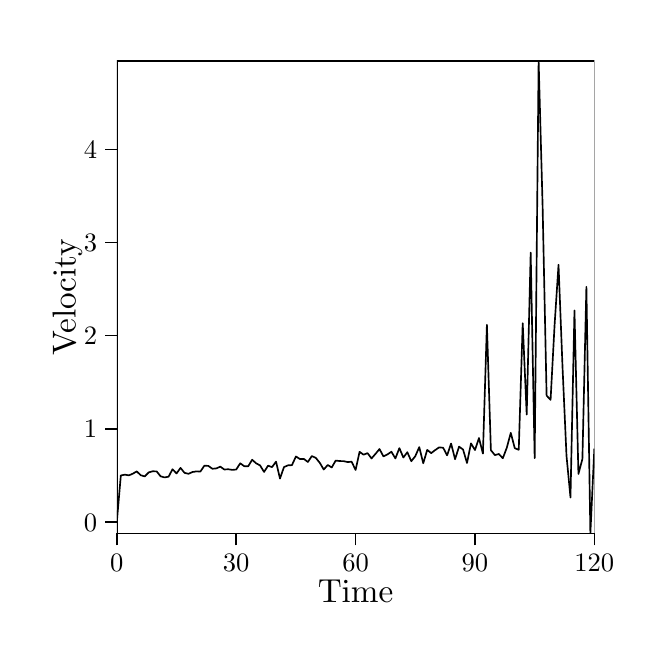
\begin{tikzpicture}[x=1pt,y=1pt]
\definecolor[named]{fillColor}{rgb}{1.00,1.00,1.00}
\path[use as bounding box,fill=fillColor,fill opacity=0.00] (0,0) rectangle (216.81,216.81);
\begin{scope}
\path[clip] (  0.00,  0.00) rectangle (216.81,216.81);
\definecolor[named]{drawColor}{rgb}{1.00,1.00,1.00}
\definecolor[named]{fillColor}{rgb}{1.00,1.00,1.00}

\path[draw=drawColor,line width= 0.6pt,line join=round,line cap=round,fill=fillColor] ( -0.00,  0.00) rectangle (216.81,216.81);
\end{scope}
\begin{scope}
\path[clip] ( 32.22, 34.03) rectangle (204.76,204.77);
\definecolor[named]{fillColor}{rgb}{1.00,1.00,1.00}

\path[fill=fillColor] ( 32.22, 34.03) rectangle (204.76,204.77);
\definecolor[named]{drawColor}{rgb}{0.00,0.00,0.00}

\path[draw=drawColor,line width= 0.6pt,line join=round] ( 32.22, 38.24) --
	( 33.66, 54.99) --
	( 35.10, 55.30) --
	( 36.54, 55.03) --
	( 37.97, 55.63) --
	( 39.41, 56.47) --
	( 40.85, 55.09) --
	( 42.29, 54.66) --
	( 43.72, 56.10) --
	( 45.16, 56.51) --
	( 46.60, 56.47) --
	( 48.04, 54.69) --
	( 49.48, 54.29) --
	( 50.91, 54.56) --
	( 52.35, 57.25) --
	( 53.79, 55.73) --
	( 55.23, 57.75) --
	( 56.67, 55.94) --
	( 58.10, 55.60) --
	( 59.54, 56.24) --
	( 60.98, 56.47) --
	( 62.42, 56.44) --
	( 63.85, 58.53) --
	( 65.29, 58.46) --
	( 66.73, 57.42) --
	( 68.17, 57.55) --
	( 69.61, 58.19) --
	( 71.04, 57.15) --
	( 72.48, 57.25) --
	( 73.92, 57.01) --
	( 75.36, 57.15) --
	( 76.80, 59.40) --
	( 78.23, 58.36) --
	( 79.67, 58.29) --
	( 81.11, 60.68) --
	( 82.55, 59.40) --
	( 83.98, 58.63) --
	( 85.42, 56.27) --
	( 86.86, 58.53) --
	( 88.30, 58.02) --
	( 89.74, 60.01) --
	( 91.17, 53.88) --
	( 92.61, 58.02) --
	( 94.05, 58.66) --
	( 95.49, 58.73) --
	( 96.93, 61.86) --
	( 98.36, 60.95) --
	( 99.80, 60.98) --
	(101.24, 59.87) --
	(102.68, 62.02) --
	(104.11, 61.35) --
	(105.55, 59.57) --
	(106.99, 57.15) --
	(108.43, 58.79) --
	(109.87, 57.89) --
	(111.30, 60.38) --
	(112.74, 60.21) --
	(114.18, 60.17) --
	(115.62, 59.84) --
	(117.06, 59.97) --
	(118.49, 56.98) --
	(119.93, 63.54) --
	(121.37, 62.50) --
	(122.81, 63.07) --
	(124.24, 61.15) --
	(125.68, 62.80) --
	(127.12, 64.55) --
	(128.56, 61.89) --
	(130.00, 62.60) --
	(131.43, 63.57) --
	(132.87, 61.15) --
	(134.31, 64.88) --
	(135.75, 61.49) --
	(137.19, 63.40) --
	(138.62, 60.14) --
	(140.06, 61.96) --
	(141.50, 65.25) --
	(142.94, 59.40) --
	(144.37, 64.24) --
	(145.81, 63.07) --
	(147.25, 64.18) --
	(148.69, 65.15) --
	(150.13, 65.02) --
	(151.56, 62.26) --
	(153.00, 66.53) --
	(154.44, 60.88) --
	(155.88, 65.42) --
	(157.32, 64.38) --
	(158.75, 59.50) --
	(160.19, 66.60) --
	(161.63, 64.18) --
	(163.07, 68.52) --
	(164.50, 62.90) --
	(165.94,109.46) --
	(167.38, 64.14) --
	(168.82, 62.36) --
	(170.26, 62.76) --
	(171.69, 61.22) --
	(173.13, 65.02) --
	(174.57, 70.40) --
	(176.01, 64.85) --
	(177.45, 64.28) --
	(178.88,110.03) --
	(180.32, 76.99) --
	(181.76,135.53) --
	(183.20, 61.25) --
	(184.63,204.77) --
	(186.07,152.28) --
	(187.51, 83.86) --
	(188.95, 82.31) --
	(190.39,109.26) --
	(191.82,131.12) --
	(193.26, 94.29) --
	(194.70, 62.13) --
	(196.14, 47.05) --
	(197.58,114.61) --
	(199.01, 55.53) --
	(200.45, 60.95) --
	(201.89,123.18) --
	(203.33, 34.03) --
	(204.76, 64.72);

\path[draw=drawColor,line width= 0.6pt,line join=round,line cap=round] ( 32.22, 34.03) rectangle (204.76,204.77);
\end{scope}
\begin{scope}
\path[clip] (  0.00,  0.00) rectangle (216.81,216.81);
\definecolor[named]{drawColor}{rgb}{0.00,0.00,0.00}

\node[text=drawColor,anchor=base east,inner sep=0pt, outer sep=0pt, scale=  0.96] at ( 25.11, 34.93) {0};

\node[text=drawColor,anchor=base east,inner sep=0pt, outer sep=0pt, scale=  0.96] at ( 25.11, 68.58) {1};

\node[text=drawColor,anchor=base east,inner sep=0pt, outer sep=0pt, scale=  0.96] at ( 25.11,102.22) {2};

\node[text=drawColor,anchor=base east,inner sep=0pt, outer sep=0pt, scale=  0.96] at ( 25.11,135.86) {3};

\node[text=drawColor,anchor=base east,inner sep=0pt, outer sep=0pt, scale=  0.96] at ( 25.11,169.50) {4};
\end{scope}
\begin{scope}
\path[clip] (  0.00,  0.00) rectangle (216.81,216.81);
\definecolor[named]{drawColor}{rgb}{0.00,0.00,0.00}

\path[draw=drawColor,line width= 0.6pt,line join=round] ( 27.95, 38.24) --
	( 32.22, 38.24);

\path[draw=drawColor,line width= 0.6pt,line join=round] ( 27.95, 71.88) --
	( 32.22, 71.88);

\path[draw=drawColor,line width= 0.6pt,line join=round] ( 27.95,105.52) --
	( 32.22,105.52);

\path[draw=drawColor,line width= 0.6pt,line join=round] ( 27.95,139.16) --
	( 32.22,139.16);

\path[draw=drawColor,line width= 0.6pt,line join=round] ( 27.95,172.81) --
	( 32.22,172.81);
\end{scope}
\begin{scope}
\path[clip] (  0.00,  0.00) rectangle (216.81,216.81);
\definecolor[named]{drawColor}{rgb}{0.00,0.00,0.00}

\path[draw=drawColor,line width= 0.6pt,line join=round] ( 32.22, 29.77) --
	( 32.22, 34.03);

\path[draw=drawColor,line width= 0.6pt,line join=round] ( 75.36, 29.77) --
	( 75.36, 34.03);

\path[draw=drawColor,line width= 0.6pt,line join=round] (118.49, 29.77) --
	(118.49, 34.03);

\path[draw=drawColor,line width= 0.6pt,line join=round] (161.63, 29.77) --
	(161.63, 34.03);

\path[draw=drawColor,line width= 0.6pt,line join=round] (204.76, 29.77) --
	(204.76, 34.03);
\end{scope}
\begin{scope}
\path[clip] (  0.00,  0.00) rectangle (216.81,216.81);
\definecolor[named]{drawColor}{rgb}{0.00,0.00,0.00}

\node[text=drawColor,anchor=base,inner sep=0pt, outer sep=0pt, scale=  0.96] at ( 32.22, 20.31) {0};

\node[text=drawColor,anchor=base,inner sep=0pt, outer sep=0pt, scale=  0.96] at ( 75.36, 20.31) {30};

\node[text=drawColor,anchor=base,inner sep=0pt, outer sep=0pt, scale=  0.96] at (118.49, 20.31) {60};

\node[text=drawColor,anchor=base,inner sep=0pt, outer sep=0pt, scale=  0.96] at (161.63, 20.31) {90};

\node[text=drawColor,anchor=base,inner sep=0pt, outer sep=0pt, scale=  0.96] at (204.76, 20.31) {120};
\end{scope}
\begin{scope}
\path[clip] (  0.00,  0.00) rectangle (216.81,216.81);
\definecolor[named]{drawColor}{rgb}{0.00,0.00,0.00}

\node[text=drawColor,anchor=base,inner sep=0pt, outer sep=0pt, scale=  1.20] at (118.49,  9.03) {Time};
\end{scope}
\begin{scope}
\path[clip] (  0.00,  0.00) rectangle (216.81,216.81);
\definecolor[named]{drawColor}{rgb}{0.00,0.00,0.00}

\node[text=drawColor,rotate= 90.00,anchor=base,inner sep=0pt, outer sep=0pt, scale=  1.20] at ( 17.30,119.40) {Velocity};
\end{scope}
\end{tikzpicture}
	
		\caption{Increasing mutation rate solution for a simulation with 100 mutations and $r=1$.}
	\end{subfigure}
	\begin{subfigure}[h]{0.5\textwidth}
		% Created by tikzDevice version 0.7.0 on 2015-03-19 12:54:23
% !TEX encoding = UTF-8 Unicode
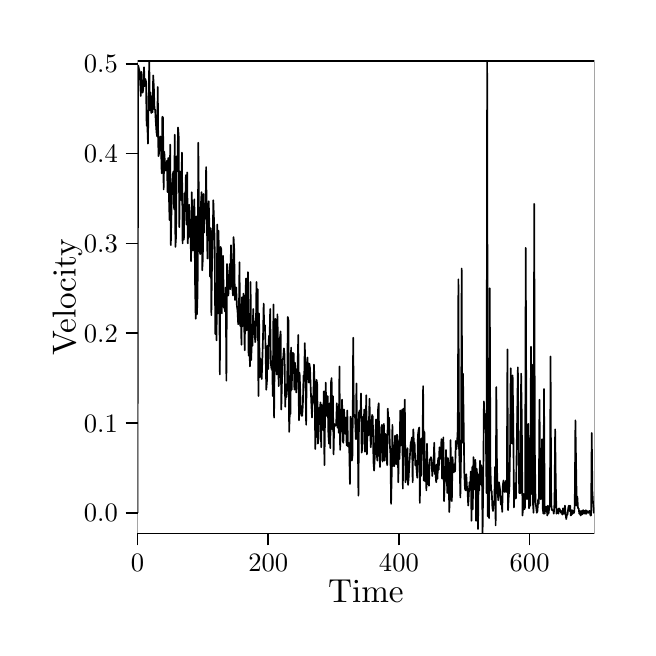
\begin{tikzpicture}[x=1pt,y=1pt]
\definecolor[named]{fillColor}{rgb}{1.00,1.00,1.00}
\path[use as bounding box,fill=fillColor,fill opacity=0.00] (0,0) rectangle (216.81,216.81);
\begin{scope}
\path[clip] (  0.00,  0.00) rectangle (216.81,216.81);
\definecolor[named]{drawColor}{rgb}{1.00,1.00,1.00}
\definecolor[named]{fillColor}{rgb}{1.00,1.00,1.00}

\path[draw=drawColor,line width= 0.6pt,line join=round,line cap=round,fill=fillColor] ( -0.00,  0.00) rectangle (216.81,216.81);
\end{scope}
\begin{scope}
\path[clip] ( 39.69, 34.03) rectangle (204.76,204.77);
\definecolor[named]{fillColor}{rgb}{1.00,1.00,1.00}

\path[fill=fillColor] ( 39.69, 34.03) rectangle (204.76,204.77);
\definecolor[named]{drawColor}{rgb}{0.00,0.00,0.00}

\path[draw=drawColor,line width= 0.6pt,line join=round] ( 39.69, 41.50) --
	( 39.92,203.14) --
	( 40.16,202.17) --
	( 40.40,201.19) --
	( 40.63,197.62) --
	( 40.87,192.11) --
	( 41.10,200.87) --
	( 41.34,193.40) --
	( 41.58,193.40) --
	( 41.81,195.03) --
	( 42.05,202.49) --
	( 42.28,195.68) --
	( 42.52,198.27) --
	( 42.76,197.30) --
	( 42.99,181.40) --
	( 43.23,181.72) --
	( 43.47,174.90) --
	( 43.70,193.08) --
	( 43.94,204.77) --
	( 44.17,186.91) --
	( 44.41,193.40) --
	( 44.65,185.94) --
	( 44.88,190.81) --
	( 45.12,186.26) --
	( 45.35,199.57) --
	( 45.59,195.68) --
	( 45.83,187.24) --
	( 46.06,187.24) --
	( 46.30,182.69) --
	( 46.54,179.12) --
	( 46.77,177.50) --
	( 47.01,195.35) --
	( 47.24,170.36) --
	( 47.48,171.33) --
	( 47.72,176.53) --
	( 47.95,177.50) --
	( 48.19,173.61) --
	( 48.42,164.19) --
	( 48.66,184.64) --
	( 48.90,184.32) --
	( 49.13,158.35) --
	( 49.37,171.98) --
	( 49.61,167.76) --
	( 49.84,165.17) --
	( 50.08,165.82) --
	( 50.31,168.74) --
	( 50.55,157.38) --
	( 50.79,169.71) --
	( 51.02,156.73) --
	( 51.26,147.31) --
	( 51.49,174.58) --
	( 51.73,138.23) --
	( 51.97,150.56) --
	( 52.20,159.32) --
	( 52.44,163.87) --
	( 52.68,164.84) --
	( 52.91,151.21) --
	( 53.15,178.15) --
	( 53.38,137.58) --
	( 53.62,141.15) --
	( 53.86,170.36) --
	( 54.09,164.84) --
	( 54.33,180.75) --
	( 54.56,177.82) --
	( 54.80,144.72) --
	( 55.04,164.84) --
	( 55.27,159.97) --
	( 55.51,154.45) --
	( 55.75,171.66) --
	( 55.98,138.87) --
	( 56.22,152.83) --
	( 56.45,140.17) --
	( 56.69,157.05) --
	( 56.93,150.56) --
	( 57.16,163.54) --
	( 57.40,145.69) --
	( 57.64,164.52) --
	( 57.87,138.87) --
	( 58.11,149.91) --
	( 58.34,152.83) --
	( 58.58,141.15) --
	( 58.82,143.09) --
	( 59.05,132.38) --
	( 59.29,157.38) --
	( 59.52,146.99) --
	( 59.76,136.28) --
	( 60.00,149.26) --
	( 60.23,154.78) --
	( 60.47,124.92) --
	( 60.71,111.61) --
	( 60.94,148.61) --
	( 61.18,113.23) --
	( 61.41,121.35) --
	( 61.65,175.23) --
	( 61.89,150.88) --
	( 62.12,136.28) --
	( 62.36,134.98) --
	( 62.59,152.83) --
	( 62.83,157.38) --
	( 63.07,129.14) --
	( 63.30,133.36) --
	( 63.54,156.73) --
	( 63.78,142.77) --
	( 64.01,150.88) --
	( 64.25,147.96) --
	( 64.48,166.46) --
	( 64.72,148.29) --
	( 64.96,133.36) --
	( 65.19,151.53) --
	( 65.43,154.13) --
	( 65.66,145.04) --
	( 65.90,126.87) --
	( 66.14,144.39) --
	( 66.37,112.91) --
	( 66.61,131.41) --
	( 66.85,140.17) --
	( 67.08,154.45) --
	( 67.32,147.64) --
	( 67.55,140.50) --
	( 67.79,106.09) --
	( 68.03,113.88) --
	( 68.26,103.82) --
	( 68.50,145.69) --
	( 68.73,113.56) --
	( 68.97,143.42) --
	( 69.21,125.57) --
	( 69.44, 91.49) --
	( 69.68,137.58) --
	( 69.92,136.93) --
	( 70.15,113.56) --
	( 70.39,128.16) --
	( 70.62,134.33) --
	( 70.86,115.83) --
	( 71.10,115.50) --
	( 71.33,114.21) --
	( 71.57,122.97) --
	( 71.80, 89.21) --
	( 72.04,131.41) --
	( 72.28,120.05) --
	( 72.51,120.05) --
	( 72.75,124.27) --
	( 72.99,131.41) --
	( 73.22,122.32) --
	( 73.46,138.23) --
	( 73.69,128.81) --
	( 73.93,123.29) --
	( 74.17,120.05) --
	( 74.40,141.15) --
	( 74.64,136.60) --
	( 74.87,118.43) --
	( 75.11,118.75) --
	( 75.35,122.97) --
	( 75.58,116.48) --
	( 75.82,114.53) --
	( 76.06,109.66) --
	( 76.29,109.99) --
	( 76.53,132.06) --
	( 76.76,109.01) --
	( 77.00,116.80) --
	( 77.24,102.20) --
	( 77.47,119.40) --
	( 77.71,109.01) --
	( 77.95,120.70) --
	( 78.18,111.93) --
	( 78.42,100.25) --
	( 78.65,116.80) --
	( 78.89,126.22) --
	( 79.13,107.39) --
	( 79.36,118.43) --
	( 79.60,128.49) --
	( 79.83, 98.30) --
	( 80.07,108.04) --
	( 80.31, 94.41) --
	( 80.54,124.92) --
	( 80.78, 96.68) --
	( 81.02,105.44) --
	( 81.25,101.87) --
	( 81.49,115.18) --
	( 81.72,106.09) --
	( 81.96,110.64) --
	( 82.20,103.17) --
	( 82.43,105.12) --
	( 82.67,124.92) --
	( 82.90,116.15) --
	( 83.14,122.32) --
	( 83.38, 83.70) --
	( 83.61,113.56) --
	( 83.85, 90.51) --
	( 84.09, 97.33) --
	( 84.32, 92.78) --
	( 84.56, 89.86) --
	( 84.79, 96.35) --
	( 85.03,104.79) --
	( 85.27,117.13) --
	( 85.50,107.39) --
	( 85.74,109.34) --
	( 85.97,100.57) --
	( 86.21, 85.97) --
	( 86.45, 88.89) --
	( 86.68,101.87) --
	( 86.92, 93.43) --
	( 87.16,105.44) --
	( 87.39,103.17) --
	( 87.63,115.18) --
	( 87.86, 95.38) --
	( 88.10, 93.43) --
	( 88.34, 96.35) --
	( 88.57, 83.70) --
	( 88.81,116.80) --
	( 89.04, 75.91) --
	( 89.28,101.87) --
	( 89.52,111.61) --
	( 89.75, 96.35) --
	( 89.99, 91.49) --
	( 90.23,113.23) --
	( 90.46,103.17) --
	( 90.70, 87.27) --
	( 90.93, 95.38) --
	( 91.17,104.79) --
	( 91.41,107.07) --
	( 91.64, 78.83) --
	( 91.88, 88.56) --
	( 92.11, 96.68) --
	( 92.35, 97.65) --
	( 92.59,100.90) --
	( 92.82, 98.63) --
	( 93.06, 79.80) --
	( 93.30, 87.92) --
	( 93.53, 83.37) --
	( 93.77, 86.62) --
	( 94.00,112.26) --
	( 94.24,110.96) --
	( 94.48, 70.71) --
	( 94.71, 77.20) --
	( 94.95, 77.20) --
	( 95.19,101.22) --
	( 95.42, 85.97) --
	( 95.66, 97.98) --
	( 95.89, 99.28) --
	( 96.13, 98.95) --
	( 96.37, 85.97) --
	( 96.60, 95.71) --
	( 96.84, 87.27) --
	( 97.07, 84.99) --
	( 97.31, 91.81) --
	( 97.55, 95.06) --
	( 97.78,105.77) --
	( 98.02, 74.93) --
	( 98.26, 92.13) --
	( 98.49, 85.64) --
	( 98.73, 77.53) --
	( 98.96, 76.55) --
	( 99.20, 76.55) --
	( 99.44, 80.45) --
	( 99.67, 91.16) --
	( 99.91, 89.21) --
	(100.14,102.85) --
	(100.38, 89.21) --
	(100.62, 73.31) --
	(100.85, 94.73) --
	(101.09, 97.65) --
	(101.33, 92.78) --
	(101.56, 88.56) --
	(101.80, 95.38) --
	(102.03, 93.76) --
	(102.27, 86.62) --
	(102.51, 80.77) --
	(102.74, 75.91) --
	(102.98, 83.70) --
	(103.21, 81.42) --
	(103.45, 95.06) --
	(103.69, 87.59) --
	(103.92, 64.55) --
	(104.16, 71.36) --
	(104.40, 89.54) --
	(104.63, 87.92) --
	(104.87, 66.49) --
	(105.10, 68.44) --
	(105.34, 79.48) --
	(105.58, 78.83) --
	(105.81, 81.42) --
	(106.05, 65.19) --
	(106.28, 80.45) --
	(106.52, 74.93) --
	(106.76, 71.36) --
	(106.99, 85.32) --
	(107.23, 58.70) --
	(107.47, 76.88) --
	(107.70, 88.56) --
	(107.94, 76.55) --
	(108.17, 76.55) --
	(108.41, 83.70) --
	(108.65, 70.06) --
	(108.88, 66.49) --
	(109.12, 81.10) --
	(109.35, 64.87) --
	(109.59, 88.56) --
	(109.83, 90.19) --
	(110.06, 71.69) --
	(110.30, 83.70) --
	(110.54, 62.60) --
	(110.77, 73.63) --
	(111.01, 72.98) --
	(111.24, 72.98) --
	(111.48, 73.63) --
	(111.72, 81.10) --
	(111.95, 72.34) --
	(112.19, 74.93) --
	(112.42, 70.39) --
	(112.66, 94.41) --
	(112.90, 64.22) --
	(113.13, 76.88) --
	(113.37, 73.63) --
	(113.61, 82.40) --
	(113.84, 67.47) --
	(114.08, 66.82) --
	(114.31, 78.83) --
	(114.55, 74.61) --
	(114.79, 70.06) --
	(115.02, 75.91) --
	(115.26, 65.84) --
	(115.50, 78.50) --
	(115.73, 65.52) --
	(115.97, 66.82) --
	(116.20, 64.55) --
	(116.44, 51.89) --
	(116.68, 76.23) --
	(116.91, 72.66) --
	(117.15, 60.33) --
	(117.38, 62.27) --
	(117.62,104.79) --
	(117.86, 76.55) --
	(118.09, 76.88) --
	(118.33, 75.58) --
	(118.57, 68.12) --
	(118.80, 88.24) --
	(119.04, 70.39) --
	(119.27, 70.71) --
	(119.51, 47.67) --
	(119.75, 77.85) --
	(119.98, 78.50) --
	(120.22, 75.91) --
	(120.45, 84.67) --
	(120.69, 63.25) --
	(120.93, 64.87) --
	(121.16, 76.23) --
	(121.40, 74.28) --
	(121.64, 78.83) --
	(121.87, 63.57) --
	(122.11, 69.41) --
	(122.34, 84.02) --
	(122.58, 62.60) --
	(122.82, 74.61) --
	(123.05, 69.41) --
	(123.29, 73.31) --
	(123.52, 82.72) --
	(123.76, 70.71) --
	(124.00, 65.19) --
	(124.23, 72.34) --
	(124.47, 76.88) --
	(124.71, 76.23) --
	(124.94, 60.00) --
	(125.18, 56.76) --
	(125.41, 61.30) --
	(125.65, 70.39) --
	(125.89, 75.26) --
	(126.12, 62.92) --
	(126.36, 60.33) --
	(126.59, 78.83) --
	(126.83, 81.10) --
	(127.07, 64.22) --
	(127.30, 58.05) --
	(127.54, 65.52) --
	(127.78, 72.34) --
	(128.01, 73.31) --
	(128.25, 60.00) --
	(128.48, 62.92) --
	(128.72, 73.63) --
	(128.96, 60.33) --
	(129.19, 70.06) --
	(129.43, 69.41) --
	(129.66, 61.95) --
	(129.90, 58.70) --
	(130.14, 79.15) --
	(130.37, 71.36) --
	(130.61, 75.91) --
	(130.85, 66.49) --
	(131.08, 62.60) --
	(131.32, 44.75) --
	(131.55, 55.46) --
	(131.79, 73.31) --
	(132.03, 58.38) --
	(132.26, 60.65) --
	(132.50, 58.38) --
	(132.74, 69.41) --
	(132.97, 61.30) --
	(133.21, 59.03) --
	(133.44, 69.74) --
	(133.68, 69.09) --
	(133.92, 52.54) --
	(134.15, 67.14) --
	(134.39, 60.97) --
	(134.62, 78.50) --
	(134.86, 65.84) --
	(135.10, 72.34) --
	(135.33, 78.83) --
	(135.57, 50.26) --
	(135.81, 79.15) --
	(136.04, 61.95) --
	(136.28, 82.40) --
	(136.51, 52.54) --
	(136.75, 64.22) --
	(136.99, 53.51) --
	(137.22, 64.87) --
	(137.46, 51.56) --
	(137.69, 54.48) --
	(137.93, 59.35) --
	(138.17, 62.92) --
	(138.40, 66.82) --
	(138.64, 67.47) --
	(138.88, 68.76) --
	(139.11, 52.54) --
	(139.35, 71.69) --
	(139.58, 65.84) --
	(139.82, 66.82) --
	(140.06, 58.70) --
	(140.29, 60.33) --
	(140.53, 57.08) --
	(140.76, 54.16) --
	(141.00, 69.41) --
	(141.24, 71.36) --
	(141.47, 72.34) --
	(141.71, 45.07) --
	(141.95, 68.12) --
	(142.18, 54.81) --
	(142.42, 68.44) --
	(142.65, 62.92) --
	(142.89, 87.27) --
	(143.13, 53.18) --
	(143.36, 70.71) --
	(143.60, 52.86) --
	(143.83, 58.05) --
	(144.07, 49.61) --
	(144.31, 66.49) --
	(144.54, 51.89) --
	(144.78, 58.70) --
	(145.02, 51.24) --
	(145.25, 60.65) --
	(145.49, 60.97) --
	(145.72, 61.62) --
	(145.96, 60.33) --
	(146.20, 54.81) --
	(146.43, 57.40) --
	(146.67, 59.68) --
	(146.90, 66.82) --
	(147.14, 55.46) --
	(147.38, 55.46) --
	(147.61, 52.54) --
	(147.85, 59.03) --
	(148.09, 53.83) --
	(148.32, 61.30) --
	(148.56, 57.08) --
	(148.79, 65.19) --
	(149.03, 62.60) --
	(149.27, 60.97) --
	(149.50, 68.12) --
	(149.74, 53.83) --
	(149.98, 60.65) --
	(150.21, 68.76) --
	(150.45, 45.72) --
	(150.68, 52.21) --
	(150.92, 53.83) --
	(151.16, 64.22) --
	(151.39, 56.11) --
	(151.63, 48.64) --
	(151.86, 61.30) --
	(152.10, 57.08) --
	(152.34, 41.82) --
	(152.57, 47.67) --
	(152.81, 67.79) --
	(153.05, 50.91) --
	(153.28, 45.72) --
	(153.52, 61.62) --
	(153.75, 57.73) --
	(153.99, 56.11) --
	(154.23, 59.03) --
	(154.46, 56.43) --
	(154.70, 67.47) --
	(154.93, 64.55) --
	(155.17, 66.82) --
	(155.41, 72.01) --
	(155.64,125.89) --
	(155.88, 64.55) --
	(156.12, 58.38) --
	(156.35, 47.02) --
	(156.59, 62.27) --
	(156.82,129.79) --
	(157.06, 66.82) --
	(157.30, 91.81) --
	(157.53, 75.26) --
	(157.77, 56.11) --
	(158.00, 50.26) --
	(158.24, 49.61) --
	(158.48, 55.46) --
	(158.71, 51.24) --
	(158.95, 49.29) --
	(159.19, 44.10) --
	(159.42, 48.64) --
	(159.66, 52.54) --
	(159.89, 51.56) --
	(160.13, 56.43) --
	(160.37, 38.58) --
	(160.60, 58.05) --
	(160.84, 42.80) --
	(161.07, 61.62) --
	(161.31, 56.76) --
	(161.55, 49.94) --
	(161.78, 60.65) --
	(162.02, 38.58) --
	(162.26, 57.40) --
	(162.49, 53.83) --
	(162.73, 35.66) --
	(162.96, 55.46) --
	(163.20, 49.61) --
	(163.44, 60.33) --
	(163.67, 51.89) --
	(163.91, 58.70) --
	(164.14, 56.43) --
	(164.38, 34.03) --
	(164.62, 52.21) --
	(164.85, 81.75) --
	(165.09, 74.61) --
	(165.33, 77.20) --
	(165.56, 70.06) --
	(165.80, 48.64) --
	(166.03,204.77) --
	(166.27, 40.20) --
	(166.51, 42.15) --
	(166.74, 39.55) --
	(166.98,122.65) --
	(167.21, 58.05) --
	(167.45, 49.61) --
	(167.69, 49.29) --
	(167.92, 43.45) --
	(168.16, 42.15) --
	(168.40, 45.72) --
	(168.63, 45.72) --
	(168.87, 58.05) --
	(169.10, 36.96) --
	(169.34, 86.94) --
	(169.58, 58.70) --
	(169.81, 49.29) --
	(170.05, 46.04) --
	(170.29, 52.54) --
	(170.52, 51.24) --
	(170.76, 49.29) --
	(170.99, 44.42) --
	(171.23, 46.69) --
	(171.47, 41.82) --
	(171.70, 51.56) --
	(171.94, 53.18) --
	(172.17, 51.89) --
	(172.41, 48.97) --
	(172.65, 51.89) --
	(172.88, 53.18) --
	(173.12, 48.97) --
	(173.36,100.57) --
	(173.59, 42.47) --
	(173.83, 47.67) --
	(174.06, 49.94) --
	(174.30, 64.22) --
	(174.54, 93.76) --
	(174.77, 81.10) --
	(175.01, 66.49) --
	(175.24, 91.16) --
	(175.48, 73.96) --
	(175.72, 43.45) --
	(175.95, 51.89) --
	(176.19, 52.21) --
	(176.43, 46.69) --
	(176.66, 61.95) --
	(176.90, 77.53) --
	(177.13, 94.08) --
	(177.37, 66.82) --
	(177.61, 48.64) --
	(177.84, 48.64) --
	(178.08, 48.64) --
	(178.31, 91.81) --
	(178.55, 75.91) --
	(178.79, 40.53) --
	(179.02, 43.12) --
	(179.26, 48.32) --
	(179.50, 42.80) --
	(179.73, 43.45) --
	(179.97,137.25) --
	(180.20, 73.31) --
	(180.44, 46.37) --
	(180.68, 71.36) --
	(180.91, 73.63) --
	(181.15, 43.12) --
	(181.38, 44.10) --
	(181.62, 44.10) --
	(181.86,101.55) --
	(182.09, 48.32) --
	(182.33, 95.06) --
	(182.57, 45.07) --
	(182.80, 41.50) --
	(183.04,153.16) --
	(183.27, 63.90) --
	(183.51, 45.39) --
	(183.75, 43.45) --
	(183.98, 41.50) --
	(184.22, 42.15) --
	(184.45, 46.37) --
	(184.69, 44.75) --
	(184.93, 82.40) --
	(185.16, 58.38) --
	(185.40, 46.37) --
	(185.64, 57.08) --
	(185.87, 68.12) --
	(186.11, 43.12) --
	(186.34, 41.18) --
	(186.58, 86.29) --
	(186.82, 41.18) --
	(187.05, 43.77) --
	(187.29, 42.15) --
	(187.53, 43.77) --
	(187.76, 40.53) --
	(188.00, 44.10) --
	(188.23, 41.18) --
	(188.47, 43.45) --
	(188.71, 44.10) --
	(188.94, 97.98) --
	(189.18, 44.75) --
	(189.41, 42.47) --
	(189.65, 42.47) --
	(189.89, 42.47) --
	(190.12, 41.18) --
	(190.36, 45.07) --
	(190.60, 71.69) --
	(190.83, 52.21) --
	(191.07, 41.18) --
	(191.30, 42.15) --
	(191.54, 42.80) --
	(191.78, 41.18) --
	(192.01, 43.12) --
	(192.25, 42.80) --
	(192.48, 42.15) --
	(192.72, 41.50) --
	(192.96, 42.15) --
	(193.19, 40.85) --
	(193.43, 43.12) --
	(193.67, 41.18) --
	(193.90, 41.18) --
	(194.14, 44.10) --
	(194.37, 41.18) --
	(194.61, 39.23) --
	(194.85, 40.85) --
	(195.08, 40.85) --
	(195.32, 43.12) --
	(195.55, 44.10) --
	(195.79, 42.15) --
	(196.03, 44.10) --
	(196.26, 40.53) --
	(196.50, 40.85) --
	(196.74, 42.47) --
	(196.97, 41.18) --
	(197.21, 42.15) --
	(197.44, 41.50) --
	(197.68, 44.10) --
	(197.92, 74.93) --
	(198.15, 60.33) --
	(198.39, 44.10) --
	(198.62, 47.34) --
	(198.86, 43.12) --
	(199.10, 43.12) --
	(199.33, 41.18) --
	(199.57, 42.15) --
	(199.81, 40.53) --
	(200.04, 42.15) --
	(200.28, 40.85) --
	(200.51, 42.15) --
	(200.75, 42.47) --
	(200.99, 41.18) --
	(201.22, 42.15) --
	(201.46, 41.18) --
	(201.69, 42.47) --
	(201.93, 41.18) --
	(202.17, 42.15) --
	(202.40, 41.82) --
	(202.64, 41.50) --
	(202.88, 42.15) --
	(203.11, 42.15) --
	(203.35, 40.53) --
	(203.58, 40.53) --
	(203.82, 70.39) --
	(204.06, 49.29) --
	(204.29, 45.07) --
	(204.53, 41.50) --
	(204.76, 43.45);

\path[draw=drawColor,line width= 0.6pt,line join=round,line cap=round] ( 39.69, 34.03) rectangle (204.76,204.77);
\end{scope}
\begin{scope}
\path[clip] (  0.00,  0.00) rectangle (216.81,216.81);
\definecolor[named]{drawColor}{rgb}{0.00,0.00,0.00}

\node[text=drawColor,anchor=base east,inner sep=0pt, outer sep=0pt, scale=  0.96] at ( 32.57, 38.19) {0.0};

\node[text=drawColor,anchor=base east,inner sep=0pt, outer sep=0pt, scale=  0.96] at ( 32.57, 70.65) {0.1};

\node[text=drawColor,anchor=base east,inner sep=0pt, outer sep=0pt, scale=  0.96] at ( 32.57,103.11) {0.2};

\node[text=drawColor,anchor=base east,inner sep=0pt, outer sep=0pt, scale=  0.96] at ( 32.57,135.57) {0.3};

\node[text=drawColor,anchor=base east,inner sep=0pt, outer sep=0pt, scale=  0.96] at ( 32.57,168.03) {0.4};

\node[text=drawColor,anchor=base east,inner sep=0pt, outer sep=0pt, scale=  0.96] at ( 32.57,200.49) {0.5};
\end{scope}
\begin{scope}
\path[clip] (  0.00,  0.00) rectangle (216.81,216.81);
\definecolor[named]{drawColor}{rgb}{0.00,0.00,0.00}

\path[draw=drawColor,line width= 0.6pt,line join=round] ( 35.42, 41.50) --
	( 39.69, 41.50);

\path[draw=drawColor,line width= 0.6pt,line join=round] ( 35.42, 73.96) --
	( 39.69, 73.96);

\path[draw=drawColor,line width= 0.6pt,line join=round] ( 35.42,106.42) --
	( 39.69,106.42);

\path[draw=drawColor,line width= 0.6pt,line join=round] ( 35.42,138.87) --
	( 39.69,138.87);

\path[draw=drawColor,line width= 0.6pt,line join=round] ( 35.42,171.33) --
	( 39.69,171.33);

\path[draw=drawColor,line width= 0.6pt,line join=round] ( 35.42,203.79) --
	( 39.69,203.79);
\end{scope}
\begin{scope}
\path[clip] (  0.00,  0.00) rectangle (216.81,216.81);
\definecolor[named]{drawColor}{rgb}{0.00,0.00,0.00}

\path[draw=drawColor,line width= 0.6pt,line join=round] ( 39.69, 29.77) --
	( 39.69, 34.03);

\path[draw=drawColor,line width= 0.6pt,line join=round] ( 86.92, 29.77) --
	( 86.92, 34.03);

\path[draw=drawColor,line width= 0.6pt,line join=round] (134.15, 29.77) --
	(134.15, 34.03);

\path[draw=drawColor,line width= 0.6pt,line join=round] (181.38, 29.77) --
	(181.38, 34.03);
\end{scope}
\begin{scope}
\path[clip] (  0.00,  0.00) rectangle (216.81,216.81);
\definecolor[named]{drawColor}{rgb}{0.00,0.00,0.00}

\node[text=drawColor,anchor=base,inner sep=0pt, outer sep=0pt, scale=  0.96] at ( 39.69, 20.31) {0};

\node[text=drawColor,anchor=base,inner sep=0pt, outer sep=0pt, scale=  0.96] at ( 86.92, 20.31) {200};

\node[text=drawColor,anchor=base,inner sep=0pt, outer sep=0pt, scale=  0.96] at (134.15, 20.31) {400};

\node[text=drawColor,anchor=base,inner sep=0pt, outer sep=0pt, scale=  0.96] at (181.38, 20.31) {600};
\end{scope}
\begin{scope}
\path[clip] (  0.00,  0.00) rectangle (216.81,216.81);
\definecolor[named]{drawColor}{rgb}{0.00,0.00,0.00}

\node[text=drawColor,anchor=base,inner sep=0pt, outer sep=0pt, scale=  1.20] at (122.23,  9.03) {Time};
\end{scope}
\begin{scope}
\path[clip] (  0.00,  0.00) rectangle (216.81,216.81);
\definecolor[named]{drawColor}{rgb}{0.00,0.00,0.00}

\node[text=drawColor,rotate= 90.00,anchor=base,inner sep=0pt, outer sep=0pt, scale=  1.20] at ( 17.30,119.40) {Velocity};
\end{scope}
\end{tikzpicture}

	\caption{Decreasing mutation rate solution for a simulation with 100 mutations and $r=1$.}
	\end{subfigure}
\end{figure}

As we can see the positive mutation rate has a near constant velocity for the propagation of the cloud. Where as the decreasing mutation rate has a declining velocity. 

This appears to be a contradiction to the previous work.

\end{document}
